% -*- Mode: LaTeX -*-

\documentclass{report}          % tried to use [twoside] to no avail
                                % --SWM
\pagestyle{headings}
\usepackage{makeidx}
% replaced with using graphics package [2007/01/05:rpg]
%\usepackage{epsfig}
\usepackage{graphicx}

\makeatletter
\renewenvironment{theindex}%
  {\chapter{\indexname}
  \begin{small}
  \parindent 0pt
  \parskip 0pt plus .3 pt
  \relax
  \let\item\@idxitem}
  {\end{small}\clearpage}
\makeatother

%% added to try to make nice bookmarks in PDF... [2005/04/12:rpg]
\ifx\pdfoutput\undefined \csname newcount\endcsname\pdfoutput \fi 
\ifcase\pdfoutput  \else 
\usepackage[pdftex]{hyperref}
\fi

%% added to try to make nice bookmarks in PDF... [2005/04/12:rpg]
\ifx\pdfoutput\undefined \csname newcount\endcsname\pdfoutput \fi 
\ifcase\pdfoutput \DeclareGraphicsExtensions{.epsi}\DeclareGraphicsRule{epsi}{eps}{*}{}
\fi

% \DeclareGraphicsExtensions{.pdf,.epsi}
% % \DeclareGraphicsRule{epsi}{eps}{*}{}

% \DeclareGraphicsRule{epsi}{eps}{*}{}

%\usepackage{times}

%% For PDF
%\renewcommand{\rmdefault}{phv}
%\renewcommand{\sfdefault}{phv}
%\renewcommand{\ttdefault}{pcr}
%\usepackage[ps2pdf,hyperindex,hypertex,
%  pdftitle={CLIM II Specification},
%  pdfauthor={various},
%  colorlinks=true,linkcolor=blue,pagecolor=blue,
%  pdfstartview=FitBV,pdfview=FitBV]{hyperref}
%% end PDF


\title{Common Lisp Interface Manager \\
       CLIM II Specification}

\author{Scott McKay ({\tt SWM@Symbolics.COM}) \\
        William York ({\tt York@Lucid.COM}) \\ 
        {\it with contributions by} \\
        {\rm John Aspinall ({\tt JGA@Symbolics.COM})} \\
        {\rm Dennis Doughty ({\tt Doughty@ILeaf.COM})} \\
        {\rm Charles Hornig ({\tt Hornig@ODI.COM})} \\
        {\rm Richard Lamson ({\tt RLamson\%UMAB.BitNet@MITVMA.MIT.EDU})} \\
        {\rm David Linden ({\tt Linden@CRL.DEC.COM})} \\
        {\rm David Moon ({\tt Moon@Cambridge.Apple.COM})} \\
        {\rm Ramana Rao ({\tt rao@PARC.Xerox.COM})} \\
        {\rm Chris Richardson ({\tt cer@Franz.COM})}}

\date{Printed \today}
\markright{CLIM II Specification}

\makeindex

\input psfig+
% -*- Mode: LaTeX; Package: CLIM-USER -*-

%%
%%  MACROS for CLIM Specs
%%

\newskip  \normalparskip        
\normalparskip = 0pc

\def\removedepth{\ifdim \prevdepth>-1000pt \vskip -\prevdepth\fi}
\def\Vskip #1!{\endgraf
               \removedepth     
               \ifdim \lastskip<#1 \ifdim \lastskip>0pc
               \removelastskip\fi 
               \vskip#1\fi}

%%
%% Basic macros
%%

\def\curly#1{$\{${\it #1\/}$\}$}
\def\star#1{#1{\rm *}}
\def\form{\curly{form}}
\def\place{\curly{place}}
\def\paren#1{\rm({\it #1\/})}
\def\brac#1{\rm[{\it #1\/}]}
\def\ttbrac#1{\tt[{\it #1\/}]}
\def\plus#1{$\hbox{#1}^+$}
\def\placeplus{ $\{${\it place}$\}^+$}
\def\lparen{{\rm (}}
\def\rparen{{\rm )}}

\def\optional{{\tt\&optional\,}}
\def\rest{{\tt\&rest\,}}
\def\key{{\tt\&key\,\hskip 0pt}}
\def\allow{{\tt\&allow-other-keys}}
\def\body{{\tt\&body\,}}

\def\arg#1{{\it #1}}

%% When you supply a default value for optional or keyword arguments,
%% use this idiom:  \key (filled \cl{t})
%% \newcommand {\cl} [1] {{\tt #1}}

%% This allows hyphenation of CL symbols at the hyphens that exist in
%% the symbol name, but noplace else, e.g., \cl{standard\-region\-union}.
%% The reason we don't use this is that the backslashes in the symbol
%% names make Tags Search next to useless.
%% \def\cl#1{{\def\-{\discretionary{-}{}{-}}\tt #1}}

%% Spiffier version that hyphenates only at hyphens, but makes hyphens
%% be active characters, so we don't break Tags Search.  Thanks to
%% Stephen Gildea for providing this.
{\catcode`\-=\active
\gdef\cl{\bgroup
  \catcode`\-=\active \def-{{\tt \char`\-}\penalty\exhyphenpenalty}%
  \@cl}}
\def\@cl#1{\texttt{#1}\egroup}

%% Use \concept when you are introducing a term for the first time, and
%% want it in the index.  Use \term after that.
\newcommand {\concept} [1] {{\sl #1}\index{#1}}
\newcommand {\term} [1] {{\sl #1}}

%%
%% Miscellaneous
%%

\long\def\comment #1 {}

\long\def\keepout #1 {}

\long\def\Issue #1 #2 {{\bf Major issue: } {\sl #2 ---~#1}}
\long\def\issue #1 #2 {{\bf Minor issue: } {\sl #2 ---~#1}}

%%
%% Definition types
%%

\def\outdent#1{\noindent\hbox to 0pc{\hskip -1.5pc #1\hss}\ignorespaces}

\newcommand {\Dodocf} [3] {\outdent{$\Rightarrow$}{\tt #1 {\it #2} \hfill\mbox{\brac{\it #3\/}}}%
                           \index{{\tt #1} #3}%
                           \Vskip\normalparskip!}
\newcommand {\Dodocv} [2] {\outdent{$\Rightarrow$}{\tt #1 \hfill\mbox{\brac{\it #2\/}}}%
                           \index{{\tt #1} #2}%
                           \Vskip\normalparskip!}

%% Use these when you want to leave some vertical whitespace afterwards
\def\Defmacro #1 #2 {\Dodocf {#1} {#2} {Macro}}
\def\Defun #1 #2 {\Dodocf {#1} {#2} {Function}}
\def\Defgeneric #1 #2 {\Dodocf {#1} {#2} {Generic~Function}}
\def\Defmethod #1 #2 {\Dodocf {#1} {#2} {Method}}
\def\Defaftermethod #1 #2 {\Dodocf {#1} {#2} {:After~Method}}
\def\Defaroundmethod #1 #2 {\Dodocf {#1} {#2} {:Around~Method}}
\def\Defvar #1 {\Dodocv {#1} {Variable}}
\def\Defconst #1 {\Dodocv {#1} {Constant}}
\def\Defprotoclass #1 {\Dodocv {#1} {Protocol~Class}}
\def\Defpredicate #1 #2 {\Dodocf {#1} {#2} {Protocol~Predicate}}
\def\Defclass #1 {\Dodocv {#1} {Class}}
\def\Definitarg #1 {\Dodocv {#1} {Initarg}}
\def\Deftype #1 {\Dodocv {#1} {Type}}
\def\Defoption #1 {\Dodocv {#1} {Option}}
\def\Defptype #1 #2 {\Dodocf {#1} {#2} {Presentation~Type}}
\def\DefptypeAbbrev #1 #2 {\Dodocf {#1} {#2} {Presentation~Type~Abbreviation}}
\def\Defcondition #1 {\Dodocv {#1} {Condition}}
\def\Deferror #1 {\Dodocv {#1} {Error Condition}}
\def\Defrestart #1 {\Dodocv {#1} {Restart}}

\newcommand {\dodocf} [3] {\outdent{$\Rightarrow$}{\tt #1 {\it #2} \hfill\mbox{\brac{\it #3\/}}}%
                           \index{{\tt #1} #3}%
                           \linebreak}
\newcommand {\dodocv} [2] {\outdent{$\Rightarrow$}{\tt #1 \hfill\mbox{\brac{\it #2\/}}}%
                           \index{{\tt #1} #2}%
                           \linebreak}

%% Use these when you don't want to leave any vertical whitespace afterwards
\def\defmacro #1 #2 {\dodocf {#1} {#2} {Macro}}
\def\defun #1 #2 {\dodocf {#1} {#2} {Function}}
\def\defgeneric #1 #2 {\dodocf {#1} {#2} {Generic~Function}}
\def\defmethod #1 #2 {\dodocf {#1} {#2} {Method}}
\def\defvar #1 {\dodocv {#1} {Variable}}
\def\defconst #1 {\dodocv {#1} {Constant}}
\def\defprotoclass #1 {\dodocv {#1} {Protocol~Class}}
\def\defpredicate #1 #2 {\dodocf {#1} {#2} {Protocol~Predicate}}
\def\defclass #1 {\dodocv {#1} {Class}}
\def\definitarg #1 {\dodocv {#1} {Initarg}}
\def\defoption #1 {\dodocv {#1} {Option}}

\def\Defcommandtable #1 {\Dodocv {#1} {Command~Table}}
\def\Defframe #1 {\Dodocv {#1} {Application~Frame}}

\def\Defgadget #1 {\Dodocv {#1} {Abstract~Gadget}}
\def\defgadget #1 {\dodocv {#1} {Abstract~Gadget}}

\def\Defspane #1 {\Dodocv {#1} {Service~Pane}}
\def\defspane #1 {\dodocv {#1} {Service~Pane}}
\def\Deflpane #1 {\Dodocv {#1} {Layout~Pane}}
\def\deflpane #1 {\dodocv {#1} {Layout~Pane}}

\def\Callback #1 #2 {\Dodocf {#1} {#2} {Callback~Generic~Function}}
\def\callback #1 #2 {\dodocf {#1} {#2} {Callback~Generic~Function}}

%%
%% Canned phrases.
%%

\def\IfYouWantClass #1 #2 #3 {If you want to create a new class that behaves
like #1 #2, it should be a subclass of \cl{#3}.  All instantiable subclasses of
\cl{#3} must obey the #2 protocol.\ }

\def\AbstractClass{This class is an abstract class, intended only to be
subclassed, not instantiated.\ }

\def\Mutable{Members of this class are mutable.\ }

\def\Immutable{Members of this class are immutable.\ }

\def\UncapturedInputs{This function does not capture any of its mutable inputs.\ }

\def\MayCaptureInputs{This function is permitted to capture its mutable inputs; the
consequences of modifying those objects are unspecified.\ }

\def\FreshOutputs{This function returns fresh objects that may be modified.\ } 

\def\ReadOnly{This function returns objects that reveal CLIM's internal state;
do not modify those objects.\ }

\def\ReadWrite{This function returns objects that reveal CLIM's internal state;
these objects may be modified.\ }

\def\NotInRelease2{{\sl This is not fully supported in Release 2.\ }} 


%% Initialize it to \psfigtrue if your DVI to PostScript converter works
\newif \ifpsfig \psfigfalse

\addtolength{\oddsidemargin}{-.5in}
\addtolength{\evensidemargin}{-.5in}
\addtolength{\textwidth}{1in}
\addtolength{\topmargin}{-.5in}
\addtolength{\textheight}{1.0in}

\begin{document}

\maketitle

\parindent 0pc
\parskip   1pc

%% Roman-numbered pages...
\renewcommand{\thepage}{\roman{page}}

\pagebreak
\tableofcontents

\pagebreak
% -*- Mode: LaTeX -*-

\vspace*{50pt}
{\huge\bf Acknowledgments}\par
\vskip 40pt

The process of designing and implementing CLIM and writing the CLIM
specification has been a long and sometimes bumpy one.  The first thanks have
to go to the people and organizations who allowed the people working on CLIM
to continue to do so, despite the obstacles.  In particular, Mark Son-Bell of
ILA; Bob Laddaga and Saiid Zarrabian at Symbolics (and before or with them,
Ken Sinclair, Rick Karash, and Mark Graffam); and Jim Vietch and Hanoch Eiron
of Franz, Inc.  have struggled with various and sometimes conflicting business
interests through the whole process.

The attendees of the CLIM coalition meetings and those who contributed to CLIM
along the way include all of those listed on the title page, but also include
Bob Kerns, John Irwin, Paul Weineke and JonL White, and Kevin Males.  Other
contributors include Mike McMahon, Paul Robertson, John Hotchkiss, Dave Lowry,
Mike Greenwald, Dave Schatsky, and Glenn Adams.  Barry Margolin and Richard
Billington, acting for the ALU, contributed useful comments as well.

Sonya Keene, Ann Hathaway, and Ellen Golden all deserve credit for improving
the quality of this specification (in part by authoring the original CLIM
documentation), as does Mark Nahabedian.

Kent Pitman provided much useful advice on the mechanics of writing a
specification, and this document improved significantly because of that.

Last but not least are the people who have continued to use CLIM for the
duration of this lengthy process.  The people at BBN (Bruce Roberts and his
group) have been a continuing source of valuable information and suggestions.
Also, Markus Fischer of Symbolics GmbH had to deal with more than his fair
share of problems, the result of using CLIM in novel ways.


\pagebreak
\setcounter{page}{1}
\renewcommand{\thepage}{\arabic{page}}

%% Now the document proper...
\part{Overview and Conventions}
% -*- Mode: LaTeX; Package: CLIM-USER -*-

\chapter {Overview of CLIM}
\label {clim-overview}

The Common Lisp Interface Manager (CLIM) is a powerful Lisp-based programming
interface that provides a layered set of portable facilities for constructing
user interfaces.  These include basic windowing, input, output, and graphics
services; stream-oriented input and output extended with facilities such as
output recording, presentations, and context sensitive input; high level
``formatted output'' facilities; application building facilities; command
processing; and a compositional toolkit similar to those found in the X world
that supports look and feel independence.

CLIM provides an API (applications programmer interface) to user interface
facilities for the Lisp application programmer.  CLIM does not compete with the
window system or toolkits of the host machine (such as Motif or OpenLook), but
rather uses their services (to the extent that it makes sense) to integrate Lisp
applications into the host's window environment.  For example, CLIM ``windows''
are mapped onto one or more host windows, and input and output operations
performed on the CLIM window are ultimately carried out by the host window
system.  CLIM will support a large number of host environments including Genera,
Motif, OpenLook, the Macintosh, CLOE-386/486, and the Next machine.

The programmer using CLIM is insulated from most of the complexities of
portability, since the Lisp-based application need only deal with CLIM objects
and functions regardless of their operating platform (that is, the combination
of Lisp system, host computer, and host window environment).  CLIM abstracts out
many of the concepts common to all window environments.  The programmer is
encouraged to think in terms of these abstractions, rather than in the specific
capabilities of a particular host system.  For example, using CLIM, the
programmer can specify the appearance of output in high-level terms and those
high-level descriptions are turned into the appropriate appearance for the given
host.  Thus, the application has the same fundamental interface across multiple
environments, although the details will differ from system to system.

Another important goal in the design and organization of CLIM is to provide a
spectrum of user interface building options, all the way from detailed,
low-level specification of ``what goes where'', to high-level user interface
specification where the programmer leaves all of the details up to CLIM.  This
allows CLIM to balance the ease of use on one hand, and versatility on the
other.  By using high level facilities, a programmer can build portable user
interfaces quickly, whereas by recombining lower level facilities he can build
his own programming and user interfaces according to his specific needs or
requirements.  For example, CLIM supports the development of applications
independent of look and feel, as well as the portable development of toolkit
libraries that define and implement a particular look and feel.

In addition, CLIM's layered design allows application programs to exclude
facilities that they do not use, or reimplement or extend any part of the
substrate.  To these ends, CLIM is specified and implemented in a layered,
modular fashion based on protocols.  Each facility documented in this
specification has several layers of interface, and each facility is
independently specified and has a documented external interface.

The facilities provided by CLIM include:

\begin{description}

\item [Geometry]  CLIM provides provides geometric objects like point,
rectangle, and transformations and functions for manipulating them.

\item [Graphics]  CLIM provides a rich set of drawing functions,
including ones for drawing complex geometric shapes, a wide variety of drawing
options (such as line thickness), a sophisticated inking model, and color.
CLIM provides full affine transforms, so that a drawing may be arbitrarily
translated, rotated, and scaled (to the extent that the underlying window
system supports the rendering of such objects).

\item [Windowing] CLIM provides a portable layer for implementing \term{sheet}
classes (types of window-like objects) that are suited to support particular
high level facilities or interfaces.  The windowing module of CLIM defines a
uniform interface for creating and managing hierarchies of these objects
regardless of their sheet class.  This layer also provides event management.

\item [Output Recording]  CLIM provides a facility for capturing all output
done to a window.  This facility provides the support for arbitrarily scrollable
windows.  In addition, this facility serves as the root for a variety of
interesting high-level tools.

\item [Formatted Output] CLIM provides a set of macros and functions that enable
programs to produce neatly formatted tabular and graphical displays with very
little effort.

\item [Context Sensitive Input] The \term{presentation type} facility of CLIM
provides the ability to associate semantics with output, such that objects may
be retrieved later by selecting their displayed representation with the pointer.
This \term{sensitivity} comes along automatically and is integrated with the
Common Lisp type system.  A mechanism for type coercion is also included,
providing the basis for powerful user interfaces.

\item [Application Building] CLIM provides a set of tools for organizing an
application's top-level user interface and command processing loops centered on
objects called frames.  CLIM provides functionality for laying out frames under
arbitrary constraints, managing command menus and/or menu bars, and associating
user interface gestures with application commands.  Using these tools,
application writers can easily and quickly construct user interfaces that can
grow flexibly from prototype to delivery.

\item [Adaptive Toolkit] CLIM provides a uniform interface to the standard
compositional toolkits available in many environments.  CLIM defines abstract
panes that are analogous to the gadgets or widgets of a toolkit like Motif or
OpenLook.  CLIM fosters look and feel independence by specifying the interface
of these abstract panes in terms of their function and not in terms of the
details of their appearance or operation.  If an application uses these
interfaces, its user interface will adapt to use whatever toolkit is available
in the host environment.  By using this facility, application programmers can
easily construct applications that will automatically conform to a variety of
user interface standards.  In addition, a portable Lisp-based implementation of
the abstract panes is provided.

\end{description}

% -*- Mode: LaTeX; Package: CLIM-USER -*-

\chapter {Conventions}
\label {conventions}

This chapter describes the conventions used in this specification and in the
CLIM software itself.


\section {Audience, Goals, and Purpose}

This document, the {\bf CLIM Release 2 Specification}, is intended for vendors.
While it does define the Application Programmer's Interface (API), that is, the
functionality that a customer/consumer would use to write an application, it
also defines the names and functionality of some internal parts of CLIM.  These
``portals'' in implementation space allow one vendor to extend, for example, the
output record mechanism and have it work with another vendor's implementation of
incremental redisplay.  We have attempted to carefully identify the appropriate
``portals'' so that the API can be implemented efficiently, but we have also
tried not to overconstrain the specification so that it restricts creativity of
implementation or the possibility for extension.  This also affects the more
sophisticated application writers who want to go a little below the published
API but still want portable applications.  This document defines which
functionality is part of the advertised API, and which is part of the internal
protocols.

In this document, we refer to three different audiences.  A CLIM \concept{user}
is a person who uses an application program that was written using CLIM.  A CLIM
\concept{programmer} is a person who writes application programs using CLIM.  A
CLIM \concept{implementor} is a programmer who implements CLIM or extends it in
some non-trivial way.


\section {Package Structure}

CLIM defines a variety of packages in order to provide its functionality.  In
general, no symbols except for the symbols in this specification should be added
to those packages.

The \cl{clim-lisp} package is intended to implement as much of the draft X3J13
Common Lisp as possible, independent of the conformance of individual vendors.
(When all Lisp vendors implement X3J13 Common Lisp, the \cl{clim-lisp} package
could be eliminated.)  \cl{clim-lisp} is the version of Common Lisp in which
CLIM is implemented and which the \cl{clim-user} package uses instead of
\cl{common-lisp}.  \cl{clim-lisp} contains only exported symbols, and is locked
in those implementations that allow package locking.

\cl{clim} is the package where the symbols specified in this specification live.
It contains only exported symbols and is locked in those implementations that
allow package locking.

\cl{clim-sys} is the package where useful ``system-like'' functionality lives,
including such things as resources and multi-processing primitives.  It contains
functionality that is not part of Common Lisp, but which is not conceptually the
province of CLIM itself.  It contains only exported symbols and is locked in
those implementations that allow package locking.

No code is written in any of the above packages, but rather code is written for
symbols in the above packages.  None of the above use any other packages (in the
sense of the \cl{:use} option to \cl{defpackage}).  A CLIM implementation might
define a \cl{clim-internals} package that uses each of the above packages, thus
getting the definition of Lisp from \cl{clim-lisp}.  It would then implement the
functionality of the symbols in \cl{clim} and \cl{clim-sys} in the
\cl{clim-internals} package.

\cl{clim-user} is a package that programmers can use if they don't wish to
create their own package.  It is the CLIM analog of \cl{common-lisp-user}.


\section {``Spread'' Point Arguments to Functions \label{spread-vs-point}}

Many functions that take point arguments come in two forms: \concept{structured}
and \concept{spread}.  Functions that take structured point arguments take the
argument as a single \cl{point} object.  Functions that take spread point
arguments take a pair of arguments that correspond to the $x$ and $y$
coordinates of the point.

Functions that take spread point arguments, or return spread point values have
an asterisk in their name, for example, \cl{draw-line*}.


\section {Immutability of Objects}

Most CLIM objects are \concept{immutable}, that is, at the protocol level none
of their components can be modified once the object is created.  Examples of
immutable objects include all of the members of the \cl{region} classes, colors
and opacities, text styles, and line styles.  Since immutable objects by
definition never change, functions in the CLIM API can safely capture immutable
objects without first copying them.  This also allows CLIM to cache immutable
objects.  Constructor functions that return immutable objects are free to either
create and return a new object, or return an already existing object.

A few CLIM objects are \concept{mutable}.  Examples of mutable objects include
streams and output records.  Some components of mutable objects can be modified
once the object has been created, usually via \cl{setf} accessors.

In CLIM, object immutability is maintained at the class level.  Throughout this
specification, the immutability or mutability of a class will be explicitly
specified.

Some immutable classes also allow \concept{interning}.  A class is said to be
interning if it guarantees that two instances that are equivalent will always be
\cl{eq}.  For example, if the class \cl{color} were interning, calling
\cl{make-rgb-color} twice with the same arguments would return \cl{eq} values.
CLIM does not specify that any class is interning, however all immutable classes
are allowed to be interning at the discretion of the implementation.

In some rare cases, CLIM will modify objects that are members of immutable
classes.  Such objects are referred to as being \concept{volatile}.  Extreme
care must be take with volatile objects.  This specification will note whenever
some object that is part of the API is volatile.


\subsection {Behavior of Interfaces}

In this specification, any interfaces that take or return mutable objects can
be classified in a few different ways.

Most functions \concept{do not capture} their mutable input objects, that is,
these functions will either not store the objects at all, or will copy any
mutable objects before storing them, or perhaps store only some of the
components of the objects.  Later modifications to those objects will not
affect the internal state of CLIM.

Some functions \concept{may capture} their mutable input objects.  That is, it
is unspecified as to whether a CLIM implementation will or will not capture the
mutable inputs to some function.  For such functions, programmers should assume
that these objects will be captured and must not modify these objects
capriciously.  Furthermore, it is unspecified what will happen if these objects
are later modified.

Some programmers might choose to create a mutable subclass of an immutable
class.  If CLIM captures an object that is a member of such a class, it is
unspecified what will happen if the programmer later modifies that object.  If a
programmer passes such an object to a CLIM function that may capture its inputs,
he is responsible for either first copying the object or ensuring that the
object does not change later.

Some functions that return mutable objects are guaranteed to create
\concept{fresh outputs}.  These objects can be modified without affecting the
internal state of CLIM.

Functions that return mutable objects that are not fresh objects fall into two
categories: those that return \concept{read-only state}, and those that return
\concept{read/write state}.  If a function returns read-only state, programmers
must not modify that object; doing so might corrupt the state of CLIM.  If a
function returns read/write state, the modification of that object is part of
CLIM's interface, and programmers are free to modify the object in ways that
``make sense''.


\section {Protocol Classes and Predicates}

CLIM supplies a set of predicates that can be called on an object to determine
whether or not that object satisfies a certain protocol.  These predicates can
be implemented in one of two ways.

The first way is that a class implementing a particular protocol will inherit
from a \concept{protocol class} that corresponds to that protocol.  A protocol
class is an ``abstract'' class with no slots and no methods (except perhaps for
some default methods), and exists only to indicate that some subclass obeys the
protocol.  In the case when a class inherits from a protocol class, the
predicate could be implemented using \cl{typep}.  All of the CLIM region,
design, sheet, and output record classes use this convention.  For example, the
presentation protocol class and predicate could be implemented in this way:

\begin{verbatim}
(defclass presentation () ())

(defun presentationp (object)
  (typep object 'presentation))
\end{verbatim}

Note that in some implementations, it may be more efficient not to use
\cl{typep}, and instead use a generic function for the predicate.  However,
simply implementing a method for the predicate that returns \term{true} is not
necessarily enough to assert that a class supports that protocol; the class must
include the protocol class as a superclass.

CLIM always provides at least one ``standard'' instantiable class that
implements each protocol.

The second way is that a class implementing a particular protocol must simply
implement a method for a predicate generic function that returns \term{true} if
and only if that class supports the protocol (otherwise, it returns
\term{false}).  Most of the CLIM stream classes use this convention.  Protocol
classes are not used in these cases because, as in the case of some of the
stream classes, the underlying Lisp implementation may not be arranged so as to
permit it.  For example, the extended input stream protocol might be implemented
in this way:

\begin{verbatim}
(defgeneric extended-input-stream-p (object))

(defmethod extended-input-stream-p ((object t)) nil)

(defmethod extended-input-stream-p ((object basic-extended-input-protocol)) t)

(defmethod extended-input-stream-p
           ((encapsulating-stream standard-encapsulating-stream))
  (with-slots (stream) encapsulating-stream
    (extended-input-stream-p stream)))
\end{verbatim}

Whenever a class inherits from a protocol class or returns \term{true} from the
protocol predicate, the class must implement methods for all of the generic
functions that make up the protocol.


\section {Specialized Arguments to Generic Functions}

Unless otherwise stated, this specification uses the following convention
for specifying which arguments to generic functions are specialized:

\begin{itemize}
\item If the generic function is a \cl{setf} function, the second argument is
the one that is intended to be specialized.

\item If the generic function is a ``mapping'' function (such as
\cl{map-over-region-set-regions}), the second argument (the object that
specifies what is being mapped over) is the one that is specialized.  The
first argument (the functional argument) is not intended to be specialized.

\item Otherwise, the first argument is the one that is intended to be
specialized.
\end{itemize}


%% Use \tt instead of \cl, such the hairy \cl macro will blow chow
\section {Multiple Value {\tt setf}}

Some functions in CLIM that return multiple values have \cl{setf} functions
associated with them.  For example, \cl{output-record-position} returns the
position of an output record as two values that correspond to the $x$ and $y$
coordinates.  In order to change the position of an output record, the
programmer would like to invoke \cl{(setf~output-record-position)}.  Normally
however, \cl{setf} only takes a single value with which to modify the specified
place.  CLIM provides a ``multiple value'' version of \cl{setf} that allows an
expression that returns multiple values to be used in updating the specified
place.  In this specification, this facility will be referred to as \cl{setf*}
in the guise of function names such as \cl{(setf* output-record-position)}, even
though \cl{setf*} is not actually a defined form.

For example, the modifying function for \cl{output-record-position} might be
called in either of the following two ways:

\begin{verbatim}
(setf (output-record-position record) (values nx ny))

(setf (output-record-position record1) (output-record-position record2))
\end{verbatim}

The second form works because \cl{output-record-position} itself returns two
values.

Some CLIM implementations may not support \cl{setf*} due to restrictions imposed
by the underlying Lisp implementation.  In this case, programmers may use
special ``setter'' function instead.  In the above example,
\cl{output-record-set-position} is the ``setter'' function.


\section {Sheet, Stream, or Medium Arguments to Macros}

There are many macros that take a sheet, stream, or medium as one of the
arguments, for example, \cl{with-new-output-record} and \cl{formatting-table}.
In CLIM, this argument must be a variable bound to a sheet, stream, or medium;
it may not be an arbitrary form that evaluates to a sheet, stream, or medium.
\cl{t} and sometimes \cl{nil} are usually allowed as special cases; this causes
the variable to be interpreted as a reference to another stream variable
(usually \cl{*standard-output*} for output macros, or \cl{*standard-input*} for
input macros).  Note that, while the variable outside the macro form and the
variable inside the body share the same name, they cannot be assumed to be the
same reference.  That is, the macro is free to create a new binding for the
variable.  Thus, the following code fragment will not necessarily affect the
value of \arg{stream} outside the \cl{formatting-table} form:

\begin{verbatim}
(formatting-table (stream)
  (setq stream some-other-stream)
  ...)
\end{verbatim}

Furthermore, for the macros that take a sheet, stream, or medium argument, the
position of that variable is always before any forms or other ``inputs''.


\section {Macros that Expand into Calls to Advertised Functions}

Some macros that take a ``body'' argument expand into a call to an advertised
function that takes a functional argument.  This functional argument will
execute the supplied body.  For a macro named ``{\it \cl{with-}environment}'',
the function is generally named ``{\it \cl{invoke-with-}environment}''.  For
example, \cl{with-drawing-options} might be defined as follows:

\begin{verbatim}
(defgeneric invoke-with-drawing-options (medium continuation &key)
  (declare (dynamic-extent continuation)))

(defmacro with-drawing-options ((medium &rest drawing-options) &body body)
  `(flet ((with-drawing-options-body (,medium) ,@body))
     (declare (dynamic-extent #'with-drawing-options-body))
     (invoke-with-drawing-options
       ,medium #'with-drawing-options-body ,@drawing-options)))

(defmethod invoke-with-drawing-options 
           ((medium clx-display-medium) continuation &rest drawing-options)
  (with-drawing-options-merged-into-medium (medium drawing-options)
    (funcall continuation medium)))
\end{verbatim}


\section {Terminology Pertaining to Error Conditions}

When this specification specifies that it ``is an error'' for some situation to
occur, this means that:

\begin{itemize}
\item No valid CLIM program should cause this situation to occur.

\item If this situation does occur, the effects and results are undefined as
far as adherence to the CLIM specification is concerned.

\item CLIM implementations are not required to detect such an error, although
implementations are encouraged to provide such error detection whenever it is
reasonable to do so.
\end{itemize}

When this specification specifies that some argument ``must be a \term{type}''
or uses the phrase ``the \term{type} \arg{argument}'', this means that it is an
error if the argument is not of the specified type.  CLIM implementations are
encouraged, but not required, to generate an argument type error for these
situations.

When this specification says that ``an error is signalled'' in some situation,
this means that:

\begin{itemize}
\item If the situation occurs, an error will be signalled using either
\cl{error} or \cl{cerror}.

\item Valid CLIM programs may rely on the fact that an error will be signalled.

\item Every CLIM implementation is required to detect such an error.
\end{itemize}

When this specification says that ``a condition is signalled'' in some
situation, this is just like ``an error is signalled'' with the exception that
the condition will be signalled using \cl{signal} instead of \cl{error}.


\part{Geometry Substrate}
% -*- Mode: LaTeX; Package: CLIM-USER -*-

\chapter {Regions}
\label {regions}

CLIM provides definitions for a variety of geometric objects, including points,
lines, elliptical arcs, regions, and transformations.  Both the graphics and
windowing modules use the same set of geometric objects and functions.  In this
section, we describe regions, points, and the basic region classes.
Transformations will be described in Chapter~\ref{transforms}.

Most of these objects are described as if they are implemented using standard
classes.  However, this need not be the case.  In particular, they may be
implemented using structure classes, and some classes may exist only to name a
place in the hierarchy---all members of such a class will be instances of that
class's subclasses.  The most important concern is that these classes must allow
specializing generic functions.

The coordinate system in which the geometric objects reside is an abstract,
continuous coordinate system.  This abstract coordinate system is converted into
``real world'' coordinates only during operations such as rendering one of the
objects on a display device.

Angles are measured in radians.  Following standard conventions, when an angle
is measured relative to a given line, a positive angle indicates an angle
counter-clockwise from the line in the plane.  When the angle from the positive
$x$ axis to the positive $y$ axis is positive (that is, the positive $y$ axis is
counter-clockwise from the positive $x$ axis), the coordinate system is said to
be \concept{right-handed}.  When this angle is negative, the coordinate system
is said to be \concept{left-handed}.  Thus, the cartesian coordinate system with
$x$ increasing to the right and $y$ increasing upward is right-handed.  A
coordinate system with $y$ increasing down is left-handed.  (By default, CLIM
streams are left handed, but no such default exists for sheets in general.)


\section {General Regions}

A \concept{region} is an object that denotes a set of mathematical points in the
plane.  Regions include their boundaries, that is, they are closed.  Regions
have infinite resolution.

A \concept{bounded region} is a region that contains at least one point and for
which there exists a number, $d$, called the region's diameter, such that if
$p1$ and $p2$ are points in the region, the distance between $p1$ and $p2$ is
always less than or equal to $d$.

An \concept{unbounded region} either contains no points or contains points
arbitrarily far apart.

Another way to describe a region is that it maps every $(x,y)$ pair into either
\term{true} or \term{false} (meaning member or not a member, respectively, of
the region).  Later, in Chapter~\ref{designs}, we will generalize a region to
something called a \concept{design} that maps every point $(x,y)$ into color and
opacity values.

\Defprotoclass {region}

The protocol class that corresponds to a set of points.  This includes both
bounded and unbounded regions.  This is a subclass of \cl{design} (see
Chapter~\ref{color}).

\IfYouWantClass {a} {region} {region}

There is no general constructor called \cl{make-region} because of the
impossibility of a uniform way to specify the arguments to such a function.

\Defpredicate {regionp} {object}

Returns \term{true} if \arg{object} is a \term{region}, otherwise returns
\term{false}.

\Defprotoclass {path}

The protocol class \cl{path} denotes bounded regions that have
\concept{dimensionality} 1 (that is, have length).  It is a subclass of
\cl{region} and \cl{bounding-rectangle}.
\IfYouWantClass {a} {path} {path}

Constructing a \cl{path} object with no length (via \cl{make-line*}, for
example) may canonicalize it to \cl{+nowhere+}.

Some rendering models support the constructing of areas by filling a closed
path.  In this case, the path needs a direction associated with it.  Since CLIM
does not currently support the path-filling model, paths are directionless.

\Defpredicate {pathp} {object}

Returns \term{true} if \arg{object} is a \term{path}, otherwise returns
\term{false}.

Note that constructing a \cl{path} object with no length (such as calling
\cl{make-line} with two coincident points), for example) may canonicalize it to
\cl{+nowhere+}.

\Defprotoclass {area}

The protocol class \cl{area} denotes bounded regions that have dimensionality 2
(that is, have area).  It is a subclass of \cl{region} and \cl{bounding-rectangle}.
\IfYouWantClass {an} {area} {area}

Note that constructing an \cl{area} object with no area (such as calling
\cl{make-rectangle} with two coincident points), for example) may canonicalize
it to \cl{+nowhere+}.

\Defpredicate {areap} {object}

Returns \term{true} if \arg{object} is an \term{area}, otherwise returns
\term{false}.

\Deftype {coordinate}

The type that represents a coordinate.  This must either be \cl{t}, or a
subtype of \cl{real}.  CLIM implementations may use a more specific subtype of
\cl{real}, such as \cl{single-float}, for reasons of efficiency.

All of the specific region classes and subclasses of \cl{bounding-rectangle}
will use this type to store their coordinates.  However, the constructor
functions for the region classes and for bounding rectangles must accept numbers
of any type and coerce them to \cl{coordinate}.

\Defun {coordinate} {n}

Coerces the number \arg{n} to be a coordinate.


\defconst {+everywhere+}
\Defconst {+nowhere+}

\cl{+everywhere+} is the region that includes all the points on the
two-dimensional infinite drawing plane. \cl{+nowhere+} is the empty region, the
opposite of \cl{+everywhere+}.


\subsection {The Region Predicate Protocol}

The following generic functions comprise the region predicate protocol.  All
classes that are subclasses of \cl{region} must either inherit or implement
methods for these generic functions.

The methods for \cl{region-equal}, \cl{region-contains-region-p}, and
\cl{region-intersects-region-p} will typically specialize both the \arg{region1}
and \arg{region2} arguments.


\Defgeneric {region-equal} {region1 region2}

Returns \term{true} if the two \term{regions} \arg{region1} and \arg{region2}
contain exactly the same set of points, otherwise returns \term{false}.

\Defgeneric {region-contains-region-p} {region1 region2}

Returns \term{true} if all points in the \term{region} \arg{region2} are members
of the \term{region} \arg{region1}, otherwise returns \term{false}.

\Defgeneric {region-contains-position-p} {region x y}

Returns \term{true} if the point at $(x,y)$ is contained in the \term{region}
\arg{region}, otherwise returns \term{false}.  Since regions in CLIM are closed,
this must return \term{true} if the point at $(x,y)$ is on the region's
boundary.  CLIM implementations are permitted to return different non-\cl{nil}
values depending on whether the point is completely inside the region or is on
the border.

\cl{region-contains-position-p} is a special case of \cl{region-contains-region-p}
in which the region is the point $(x,y)$.

\Defgeneric {region-intersects-region-p} {region1 region2}

Returns \term{false} if \cl{region-intersection} of the two \term{regions}
\arg{region1} and \arg{region2} would be \cl{+nowhere+}, otherwise returns
\term{true}.


\subsection {Region Composition Protocol}

Region composition is not always equivalent to simple set operations.  Instead,
composition attempts to return an object that has the same dimensionality as one
of its arguments.  If this is not possible, then the result is defined to be an
empty region, which is canonicalized to \cl{+nowhere+}.  (The exact details of
this are specified with each function.)

Sometimes, composition of regions can produce a result that is not a simple
contiguous region.  For example, \cl{region-union} of two rectangular regions
might not be a single rectangle.  In order to support cases like this, CLIM has
the concept of a \concept{region set}, which is an object that represents one or
more \cl{region} objects related by some region operation, usually a union.
CLIM provides standard classes to cover the cases of region union, intersection,
and difference.

Some CLIM implementations might only implement a subset of full region
composition.  Because of the importance of rectangular regions and region sets
that are the union of rectangular regions, every CLIM implementation is required
to fully support all functions that use regions for those cases.  (For example,
CLIM implementations must be able do clipping and repainting on region sets
composed entirely of axis-aligned rectangles.)  If a CLIM implementation does
not support some functions on non-rectangular region sets (for example,
clipping), it must signal an error when an unsupported case is encountered;
the exact details of this depend on the particular CLIM implementation.

\Defprotoclass {region-set}

The protocol class that represents a region set; a subclass of \cl{region} and
\cl{bounding-rectangle}.

In addition to the three classes below, there may be other instantiable
subclasses of \cl{region-set} that represent special cases, for instance, some
implementations might have a \cl{standard-rectangle-set} class that represents
the union of several axis-aligned rectangles.

\Immutable

\Defpredicate {region-set-p} {object}

Returns \term{true} if \arg{object} is a \term{region set}, otherwise returns
\term{false}.

\defclass {standard-region-union}
\defclass {standard-region-intersection}
\Defclass {standard-region-difference}

These three instantiable classes respectively implement the union, intersection,
and differences of regions.  Implementations may, but are not required to, take
advantage of the commutativity and associativity of union and intersection in
order to ``collapse'' complicated region sets into simpler ones.

Region sets that are composed entirely of axis-aligned rectangles must be
canonicalized into either a single rectangle or a union of rectangles.
Furthermore, the rectangles in the union must not overlap each other.


The following generic functions comprise the region composition protocol.  All
classes that are subclasses of \cl{region} must implement methods for these
generic functions.

The methods for \cl{region-union}, \cl{region-intersection}, and
\cl{region-difference} will typically specialize both the \arg{region1} and
\arg{region2} arguments.


\Defgeneric {region-set-regions} {region \key normalize}

Returns a sequence of the regions in the \term{region set} \arg{region}.
\arg{region} can be either a \term{region set} or a ``simple'' region, in which
case the result is simply a sequence of one element: \arg{region}.
\ReadOnly

For the case of region sets that are unions of axis-aligned rectangles, the
rectangles returned by \cl{region-set-regions} are guaranteed not to overlap.

If \arg{normalize} is supplied, it must be either \cl{:x-banding} or
\cl{:y-banding}.  If it is \cl{:x-banding} and all the regions in \arg{region}
are axis-aligned rectangles, the result is normalized by merging adjacent
rectangles with banding done in the $x$ direction.  If it is \cl{:y-banding} and
all the regions in \arg{region} are rectangles, the result is normalized with
banding done in the $y$ direction.  Normalizing a region set that is not
composed entirely of axis-aligned rectangles using x- or y-banding causes CLIM
to signal the \cl{region-set-not-rectangular} error.

\Defgeneric {map-over-region-set-regions} {function region \key normalize}

Calls \arg{function} on each region in the \term{region set} \arg{region}.  This
is often more efficient than calling \cl{region-set-regions}.  \arg{function} is
a function of one argument, a region; it has dynamic extent.  \arg{region} can
be either a \term{region set} or a ``simple'' region, in which case
\arg{function} is called once on \arg{region} itself.  \arg{normalize} is as for
\cl{region-set-regions}.


\begin{figure}
\centerline{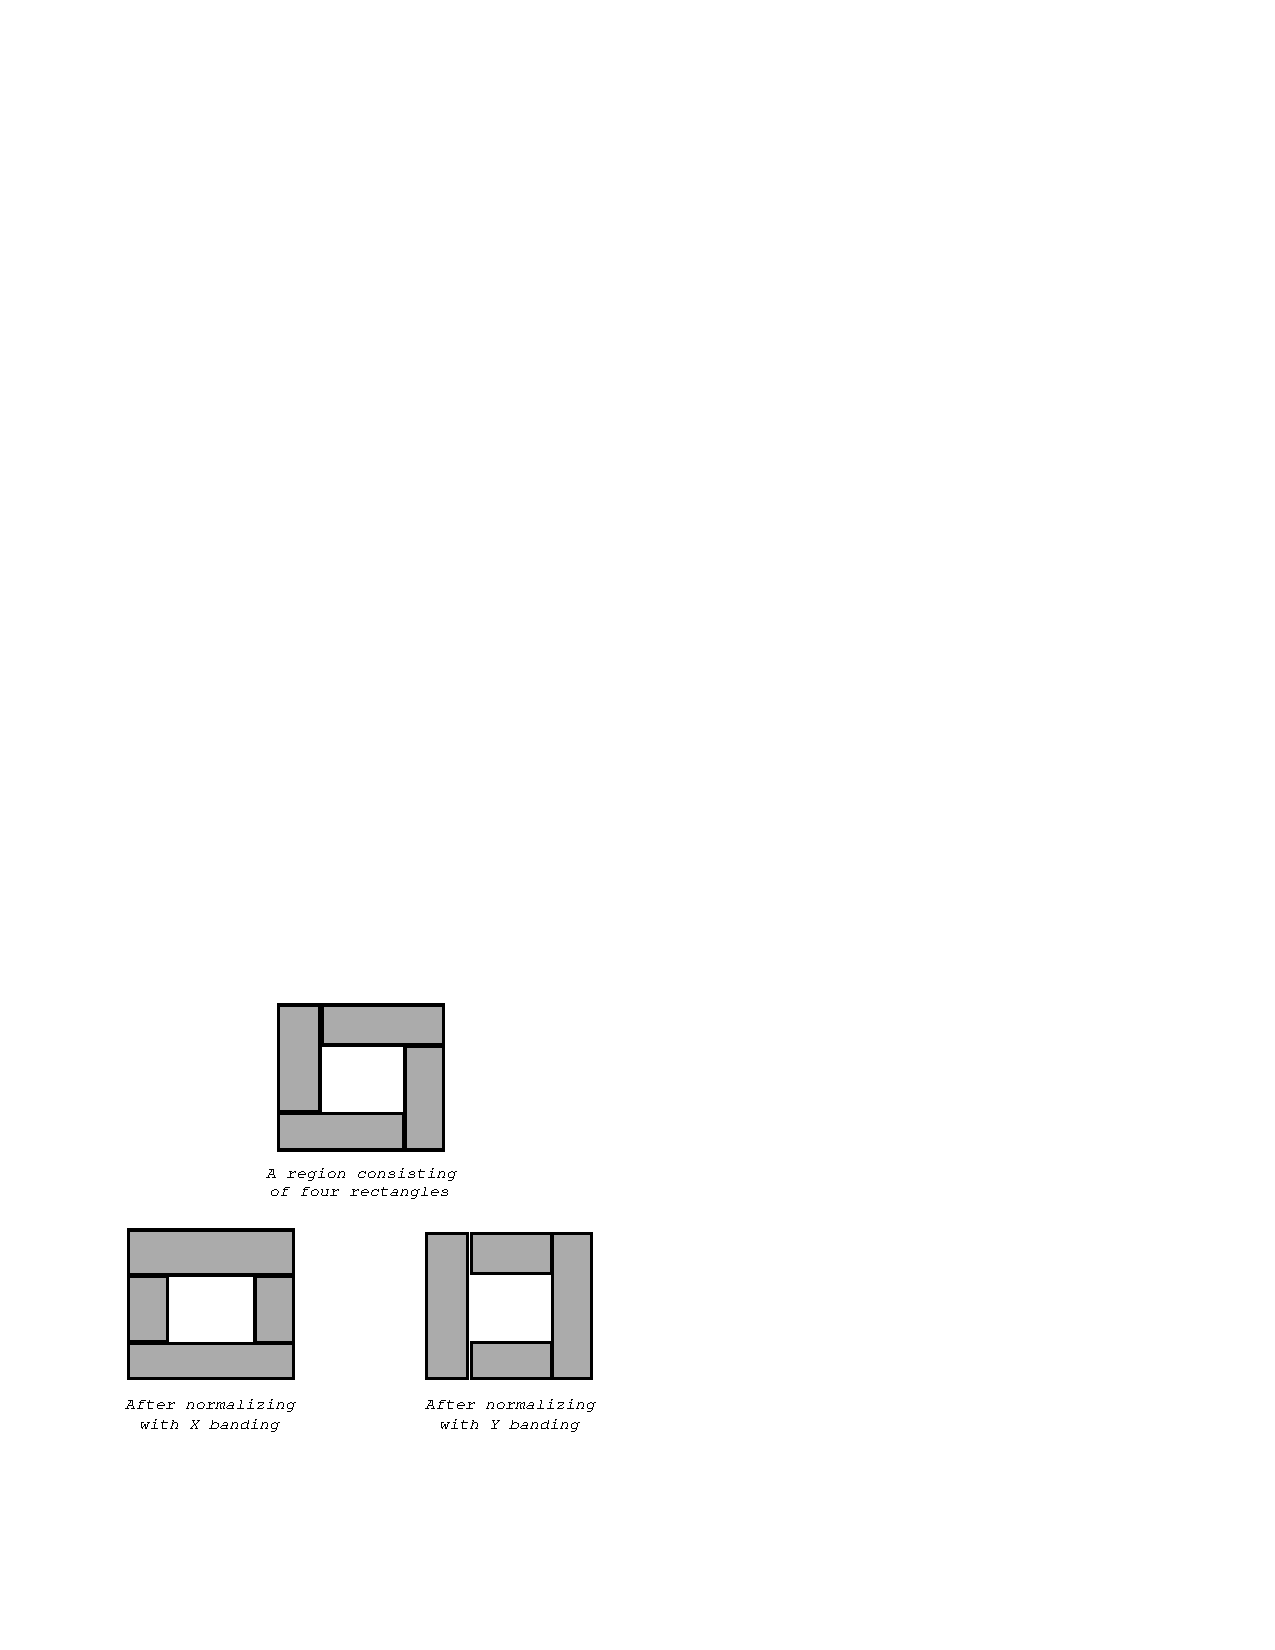
\includegraphics{region-normalization}}
\caption{Normalization of rectangular region sets.}
\end{figure}


\Defgeneric {region-union} {region1 region2}

Returns a region that contains all points that are in either of the
\term{regions} \arg{region1} or \arg{region2} (possibly with some points removed
in order to satisfy the dimensionality rule).  The result of \cl{region-union}
always has dimensionality that is the maximum dimensionality of \arg{region1}
and \arg{region2}.  For example, the union of a path and an area produces an
area; the union of two paths is a path.

\cl{region-union} will return either a simple region, a region set, or a member
of the class \cl{standard-region-union}.

\MayCaptureInputs

\Defgeneric {region-intersection} {region1 region2}

Returns a region that contains all points that are in both of the \term{regions}
\arg{region1} and \arg{region2} (possibly with some points removed in order to
satisfy the dimensionality rule).  The result of \cl{region-intersection} has
dimensionality that is the minimum dimensionality of \arg{region1} and
\arg{region2}, or is \cl{+nowhere+}.  For example, the intersection of two areas
is either another area or \cl{+nowhere+}; the intersection of two paths is
either another path or \cl{+nowhere+}; the intersection of a path and an area
produces the path clipped to stay inside of the area.

\cl{region-intersection} will return either a simple region or a member of the
class \cl{standard-region-intersection}.

\MayCaptureInputs

\Defgeneric {region-difference} {region1 region2}

Returns a region that contains all points in the \term{region} \arg{region1}
that are not in the \term{region} \arg{region2} (possibly plus additional
boundary points to make the result closed).  The result of
\cl{region-difference} has the same dimensionality as \arg{region1}, or is
\cl{+nowhere+}.  For example, the difference of an area and a path produces the
same area; the difference of a path and an area produces the path clipped to
stay outside of the area.

\cl{region-difference} will return either a simple region, a region set, or a
member of the class \cl{standard-region-difference}.

\MayCaptureInputs


\begin{figure}
\centerline{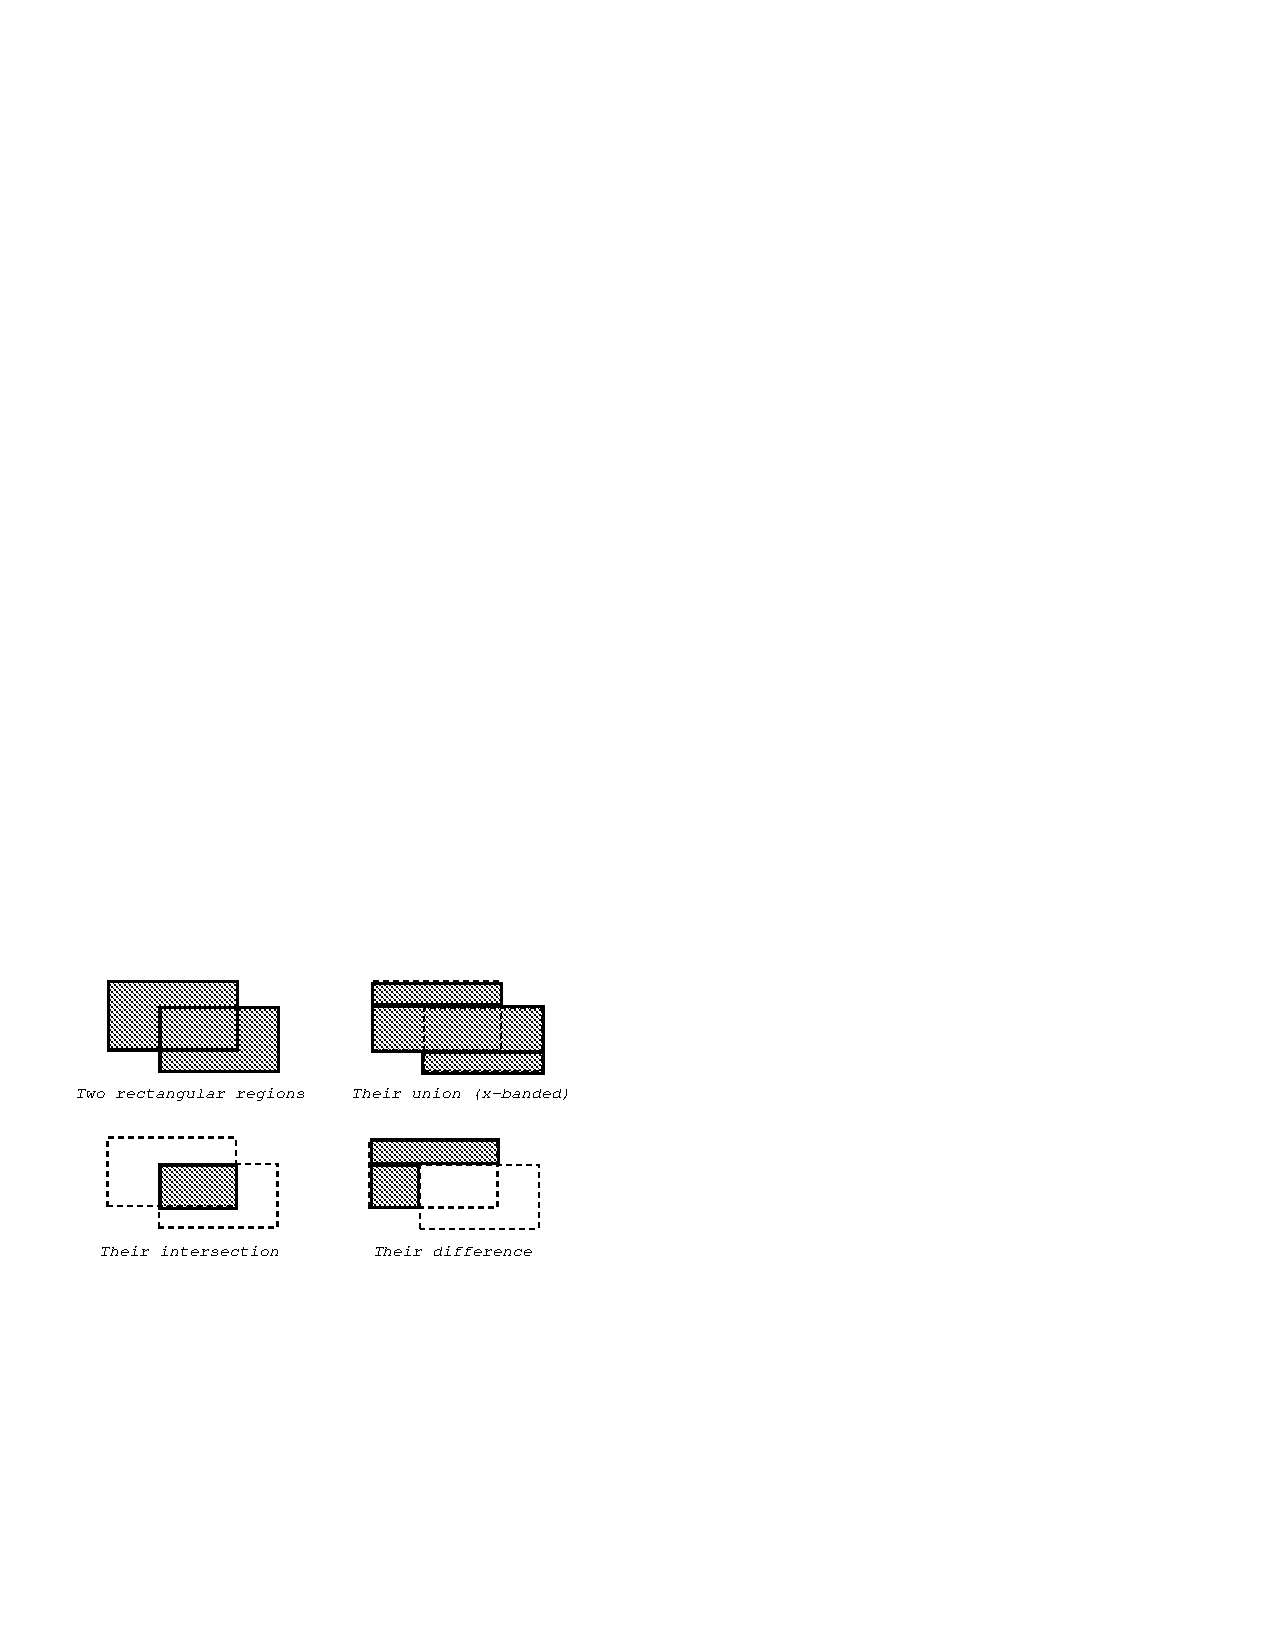
\includegraphics{region-composition}}
\caption{Examples of region union, intersection, and difference.}
\end{figure}


\section {Other Region Types}

The other types of regions are points, polylines, polygons, elliptical arcs, and
ellipses.  All of these region types are closed under affine transformations.

\Issue {SWM, York} {There is a proposal to remove the \cl{polygon},
\cl{polyline}, \cl{line}, \cl{ellipse}, and \cl{elliptical-arc} classes, since
they are only of limited utility, and CLIM itself doesn't use the classes at
all.  The advantage of removing these classes is that both the spec and CLIM
itself become a little simpler, and there are fewer cases of the region protocol
to implement.  However, removing these classes results in a geometric model that
is no longer closed (in the mathematical sense).  This lack of closure makes it
difficult to specify the design-based drawing model.  Furthermore, these are
intuitive objects that are used by a small, but important, class of
applications, and some people feel that CLIM should relieve programmers from
having to implement these classes for himself or herself.

The advocates of of removing these classes also propose removing the
design-based drawing model.  In this case, a more consistent proposal is to
remove all of the geometric classes, including \cl{point} and \cl{rectangle}.

Again, the opposing point of view believes that the power and flexibility of the
design-based drawing model does not justify the removal of any of these classes.
One counter-proposal is to require CLIM not to use any of the extended region
classes internally, and to move the implementation of the extended region
classes to a separately loadable module (via \cl{provide} and \cl{require}).}

\begin{figure}
\centerline{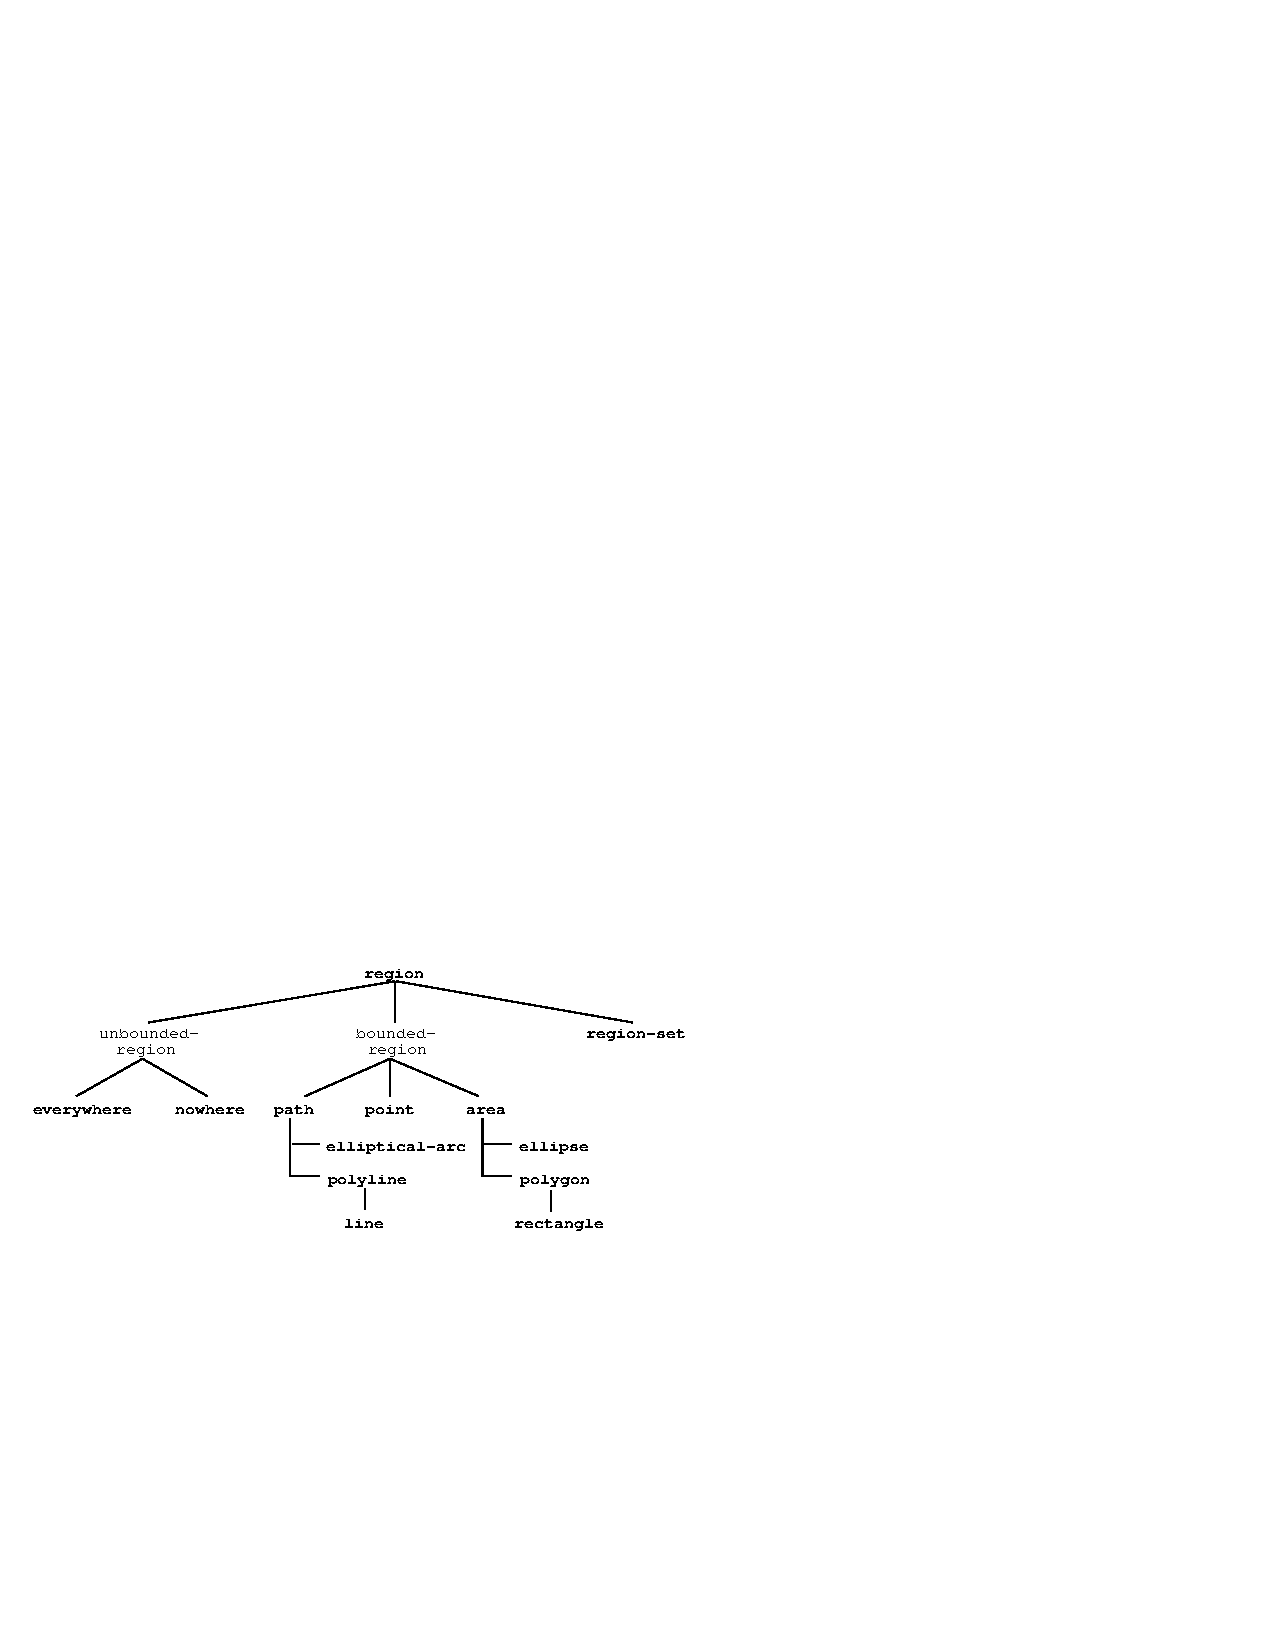
\includegraphics{region-structure}}
\caption{The class structure for all regions.}
\end{figure}


\subsection {Points}

A \concept{point} is a mathematical point in the plane, designated by its
coordinates, which are a pair of real numbers (where a real number is defined as
either an integer, a ratio, or a floating point number).  Points have neither
area nor length (that is, they have dimensionality 0).

Note well that a point is {\sl not} a pixel; CLIM models a drawing plane with
continuous coordinates.  This is discussed in more detail in
Chapter~\ref{graphics}.

\Defprotoclass {point}

The protocol class that corresponds to a mathematical point.  This is a subclass
of \cl{region} and \cl{bounding-rectangle}.
\IfYouWantClass {a} {point} {point}

\Defpredicate {pointp} {object}

Returns \term{true} if \arg{object} is a \term{point}, otherwise returns
\term{false}.

\Defclass {standard-point}

An instantiable class that implements a point.  This is a subclass of \cl{point}.
This is the class that \cl{make-point} instantiates.  
\Immutable

\Defun {make-point} {x y}

Returns an object of class \cl{standard-point} whose coordinates are \arg{x} and
\arg{y}.  \arg{x} and \arg{y} must be real numbers.


\subsubsection {The Point Protocol}

The following generic functions comprise the point API.  Only
\cl{point-position} is in the point protocol, that is, all classes that are
subclasses of \cl{point} must implement methods for \cl{point-position}, but
need not implement methods for \cl{point-x} and \cl{point-y}.

\Defgeneric {point-position} {point}

Returns both the $x$ and $y$ coordinates of the point \arg{point} as two values.

\defgeneric {point-x} {point}
\Defgeneric {point-y} {point}

Returns the $x$ or $y$ coordinate of the \term{point} \arg{point}, respectively.
CLIM will supply default methods for \cl{point-x} and \cl{point-y} on the
protocol class \cl{point} that are implemented by calling \cl{point-position}.


\subsection {Polygons and Polylines}

A \concept{polyline} is a path that consists of one or more line segments joined
consecutively at their end-points.

Polylines that have the end-point of their last line segment coincident with the
start-point of their first line segment are called \concept{closed}; this use of
the term ``closed'' should not be confused with closed sets of points.

A \concept{polygon} is an area bounded by a closed polyline. 

If the boundary of a polygon intersects itself, the odd-even winding-rule
defines the polygon: a point is inside the polygon if a ray from the point to
infinity crosses the boundary an odd number of times.

\Defprotoclass {polyline}

The protocol class that corresponds to a polyline.  This is a subclass of
\cl{path}.
\IfYouWantClass {a} {polyline} {polyline}

\Defpredicate {polylinep} {object}

Returns \term{true} if \arg{object} is a \term{polyline}, otherwise returns
\term{false}.

\Defclass {standard-polyline}

An instantiable class that implements a polyline.  This is a subclass of
\cl{polyline}.  This is the class that \cl{make-polyline} and
\cl{make-polyline*} instantiate.
\Immutable

\defun {make-polyline}  {point-seq \key closed}
\Defun {make-polyline*} {coord-seq \key closed}

Returns an object of class \cl{standard-polyline} consisting of the segments
connecting each of the points in \arg{point-seq} (or the points represented by
the coordinate pairs in \arg{coord-seq}).  \arg{point-seq} is a sequence of
\term{points}; \arg{coord-seq} is a sequence of coordinate pairs, which are real
numbers.  It is an error if \arg{coord-seq} does not contain an even number of
elements.

If \arg{closed} is \term{true}, then the segment connecting the first point and
the last point is included in the polyline.  The default for \arg{closed} is
\term{false}.

\MayCaptureInputs


\Defprotoclass {polygon}

The protocol class that corresponds to a mathematical polygon.  This is a
subclass of \cl{area}.
\IfYouWantClass {a} {polygon} {polygon}

\Defpredicate {polygonp} {object}

Returns \term{true} if \arg{object} is a \term{polygon}, otherwise returns
\term{false}.

\Defclass {standard-polygon}

An instantiable class that implements a polygon.  This is a subclass of
\cl{polygon}.  This is the class that \cl{make-polygon} and \cl{make-polygon*}
instantiate.
\Immutable

\defun {make-polygon}  {point-seq}
\Defun {make-polygon*} {coord-seq}

Returns an object of class \cl{standard-polygon} consisting of the area
contained in the boundary that is specified by the segments connecting each of
the points in \arg{point-seq} (or the points represented by the coordinate pairs
in \arg{coord-seq}).  \arg{point-seq} is a sequence of \term{points};
\arg{coord-seq} is a sequence of coordinate pairs, which are real numbers.  It
is an error if \arg{coord-seq} does not contain an even number of elements.

\MayCaptureInputs


\subsubsection {The Polygon and Polyline Protocol}

The following generic functions comprise the polygon and polyline protocol.  All
classes that are subclasses of either \cl{polygon} or \cl{polyline} must
implement methods for these generic functions.  Some of the functions below take
an argument named \arg{polygon-or-polyline}; this argument may be either a
\term{polygon} or a \term{polyline}.

\Defgeneric {polygon-points} {polygon-or-polyline}

Returns a sequence of points that specify the segments in \arg{polygon-or-polyline}.
\ReadOnly

\Defgeneric {map-over-polygon-coordinates} {function polygon-or-polyline}

Applies \arg{function} to all of the coordinates of the vertices of
\arg{polygon-or-polyline}.  \arg{function} is a function of two arguments, the
$x$ and $y$ coordinates of the vertex; it has dynamic extent.

\Defgeneric {map-over-polygon-segments} {function polygon-or-polyline}

Applies \arg{function} to the segments that compose \arg{polygon-or-polyline}.
\arg{function} is a function of four arguments, the $x$ and $y$ coordinates of
the start of the segment, and the $x$ and $y$ coordinates of the end of the
segment; it has dynamic extent.  When \cl{map-over-polygon-segments} is called
on a closed polyline, it will call \arg{function} on the segment that connects
the last point back to the first point.

\Defgeneric {polyline-closed} {polyline}

Returns \term{true} if the polyline \arg{polyline} is closed, otherwise returns
\term{false}.  This function need be implemented only for \term{polylines}, not
for \term{polygons}.


\subsection {Lines}

A line is a polyline consisting of a single segment.

\Defprotoclass {line}

The protocol class that corresponds to a mathematical line segment, that is, a
polyline with only a single segment.  This is a subclass of \cl{polyline}.
\IfYouWantClass {a} {line} {line}

\Defpredicate {linep} {object}

Returns \term{true} if \arg{object} is a \term{line}, otherwise returns
\term{false}.

\Defclass {standard-line}

An instantiable class that implements a line segment.  This is a subclass of
\cl{line}.  This is the class that \cl{make-line} and \cl{make-line*}
instantiate.
\Immutable

\defun {make-line}  {start-point end-point}
\Defun {make-line*} {start-x start-y end-x end-y}

Returns an object of class \cl{standard-line} that connects the two
\term{points} \arg{start-point} and \arg{end-point} (or the positions
(\arg{start-x},\arg{start-y}) and (\arg{end-x},\arg{end-y})).

\MayCaptureInputs


\subsubsection {The Line Protocol}

The following generic functions comprise the line API.  Only
\cl{line-start-point*} and \cl{line-end-point*} are in the line protocol, that
is, all classes that are subclasses of \cl{line} must implement methods for
\cl{line-start-point*} and \cl{line-end-point*}, but need not implement methods
for \cl{line-start-point} and \cl{line-end-point}.

\defgeneric {line-start-point*} {line}
\Defgeneric {line-end-point*}   {line}

Returns the starting or ending point, respectively, of the \term{line}
\arg{line} as two real numbers representing the coordinates of the point.

\defgeneric {line-start-point} {line}
\Defgeneric {line-end-point}   {line}

Returns the starting or ending point of the \term{line} \arg{line},
respectively.

CLIM will supply default methods for \cl{line-start-point} and
\cl{line-end-point} on the protocol class \cl{line} that are implemented by
calling \cl{line-start-point*} and \cl{line-end-point*}.


\subsection {Rectangles} 
\label {rect}

Rectangles whose edges are parallel to the coordinate axes are a special case of
polygon that can be specified completely by four real numbers
(\arg{x1},\arg{y1},\arg{x2},\arg{y2}).  They are {\sl not} closed under general
affine transformations (although they are closed under rectilinear
transformations).

\Defprotoclass {rectangle}

The protocol class that corresponds to a mathematical rectangle, that is,
rectangular polygons whose sides are parallel to the coordinate axes.  This is a
subclass of \cl{polygon}.
\IfYouWantClass {a} {rectangle} {rectangle}

\Defpredicate {rectanglep} {object}

Returns \term{true} if \arg{object} is a \term{rectangle}, otherwise returns
\term{false}.

\Defclass {standard-rectangle}

An instantiable class that implements an axis-aligned rectangle.  This is a
subclass of \cl{rectangle}.  This is the class that \cl{make-rectangle} and
\cl{make-rectangle*} instantiate.
\Immutable

\defun {make-rectangle}  {point1 point2}
\Defun {make-rectangle*} {x1 y1 x2 y2}

Returns an object of class \cl{standard-rectangle} whose edges are parallel to
the coordinate axes.  One corner is at the \term{point} \arg{point1} (or the
position (\arg{x1},\arg{y1})) and the opposite corner is at the \term{point}
\arg{point2} (or the position (\arg{x2},\arg{y2})).  There are no ordering
constraints among \arg{point1} and \arg{point2} (or \arg{x1} and \arg{x2}, and
\arg{y1} and \arg{y2}).

Most CLIM implementations will choose to represent rectangles in the most
efficient way, such as by storing the coordinates of two opposing corners of the
rectangle.  Because this representation is not sufficient to represent the
result of arbitrary transformations of arbitrary rectangles, CLIM is allowed to
return a polygon as the result of such a transformation.  (The most general
class of transformations that is guaranteed to always turn a rectangle into
another rectangle is the class of transformations that satisfy
\cl{rectilinear-transformation-p}.)

\MayCaptureInputs


\subsubsection {The Rectangle Protocol}

The following generic functions comprise the rectangle API.  Only
\cl{rectangle-edges*} is in the rectangle protocol, that is, all classes that
are subclasses of \cl{rectangle} must implement methods for
\cl{rectangle-edges*}, but need not implement methods for the remaining
functions.

\Defgeneric {rectangle-edges*} {rectangle}

Returns the coordinates of the minimum $x$ and $y$ and maximum $x$ and $y$ of
the rectangle \arg{rectangle} as four values, \arg{min-x}, \arg{min-y},
\arg{max-x}, and \arg{max-y}.

\defgeneric {rectangle-min-point} {rectangle}
\Defgeneric {rectangle-max-point} {rectangle}

Returns the min point and max point of the \term{rectangle} \arg{rectangle},
respectively.  The position of a rectangle is specified by its min point.

CLIM will supply default methods for \cl{rectangle-min-point} and
\cl{rectangle-max-point} on the protocol class \cl{rectangle} that are
implemented by calling \cl{rectangle-edges*}.


\defgeneric {rectangle-min-x} {rectangle}
\defgeneric {rectangle-min-y} {rectangle}
\defgeneric {rectangle-max-x} {rectangle}
\Defgeneric {rectangle-max-y} {rectangle}

Returns (respectively) the minimum $x$ and $y$ coordinate and maximum $x$ and
$y$ coordinate of the \term{rectangle} \arg{rectangle}.

CLIM will supply default methods for these four generic functions on the
protocol class \cl{rectangle} that are implemented by calling
\cl{rectangle-edges*}.


\defgeneric {rectangle-width}  {rectangle}
\defgeneric {rectangle-height} {rectangle}
\Defgeneric {rectangle-size}   {rectangle}

\cl{rectangle-width} returns the width of the \term{rectangle} \arg{rectangle},
which is the difference between the maximum $x$ and its minimum $x$.
\cl{rectangle-height} returns the height, which is the difference between the
maximum $y$ and its minimum $y$.  \cl{rectangle-size} returns two values, the
width and the height.

CLIM will supply default methods for these four generic functions on the
protocol class \cl{rectangle} that are implemented by calling
\cl{rectangle-edges*}.


\subsection {Ellipses and Elliptical Arcs}

An \concept{ellipse} is an area that is the outline and interior of an ellipse.
Circles are special cases of ellipses.

An \concept{elliptical arc} is a path consisting of all or a portion of the
outline of an ellipse.  Circular arcs are special cases of elliptical arcs.

An ellipse is specified in a manner that is easy to transform, and treats all
ellipses on an equal basis.  An ellipse is specified by its center point and two
vectors that describe a bounding parallelogram of the ellipse.  The bounding
parallelogram is made by adding and subtracting the vectors from the center
point in the following manner:

\begin{tabular}{|c|cc|}
 \hline
   & {\sl $x$ coordinate} & {\sl $y$ coordinate} \\
 \hline
 Center of Ellipse & $x_c$ & $y_c$ \\
 \hline
 Vectors & $dx_1$ & $dy_1$ \\
         & $dx_2$ & $dy_2$ \\
 \hline
 Corners of Parallelogram & $x_c + dx_1 + dx_2$ & $y_c + dy_1 + dy_2$ \\
                          & $x_c + dx_1 - dx_2$ & $y_c + dy_1 - dy_2$ \\
                          & $x_c - dx_1 - dx_2$ & $y_c - dy_1 - dy_2$ \\
                          & $x_c - dx_1 + dx_2$ & $y_c - dy_1 + dy_2$ \\
 \hline
\end{tabular}

Note that several different parallelograms specify the same ellipse.  One
parallelogram is bound to be a rectangle---the vectors will be perpendicular
and correspond to the semi-axes of the ellipse.

\begin{figure}
\centerline{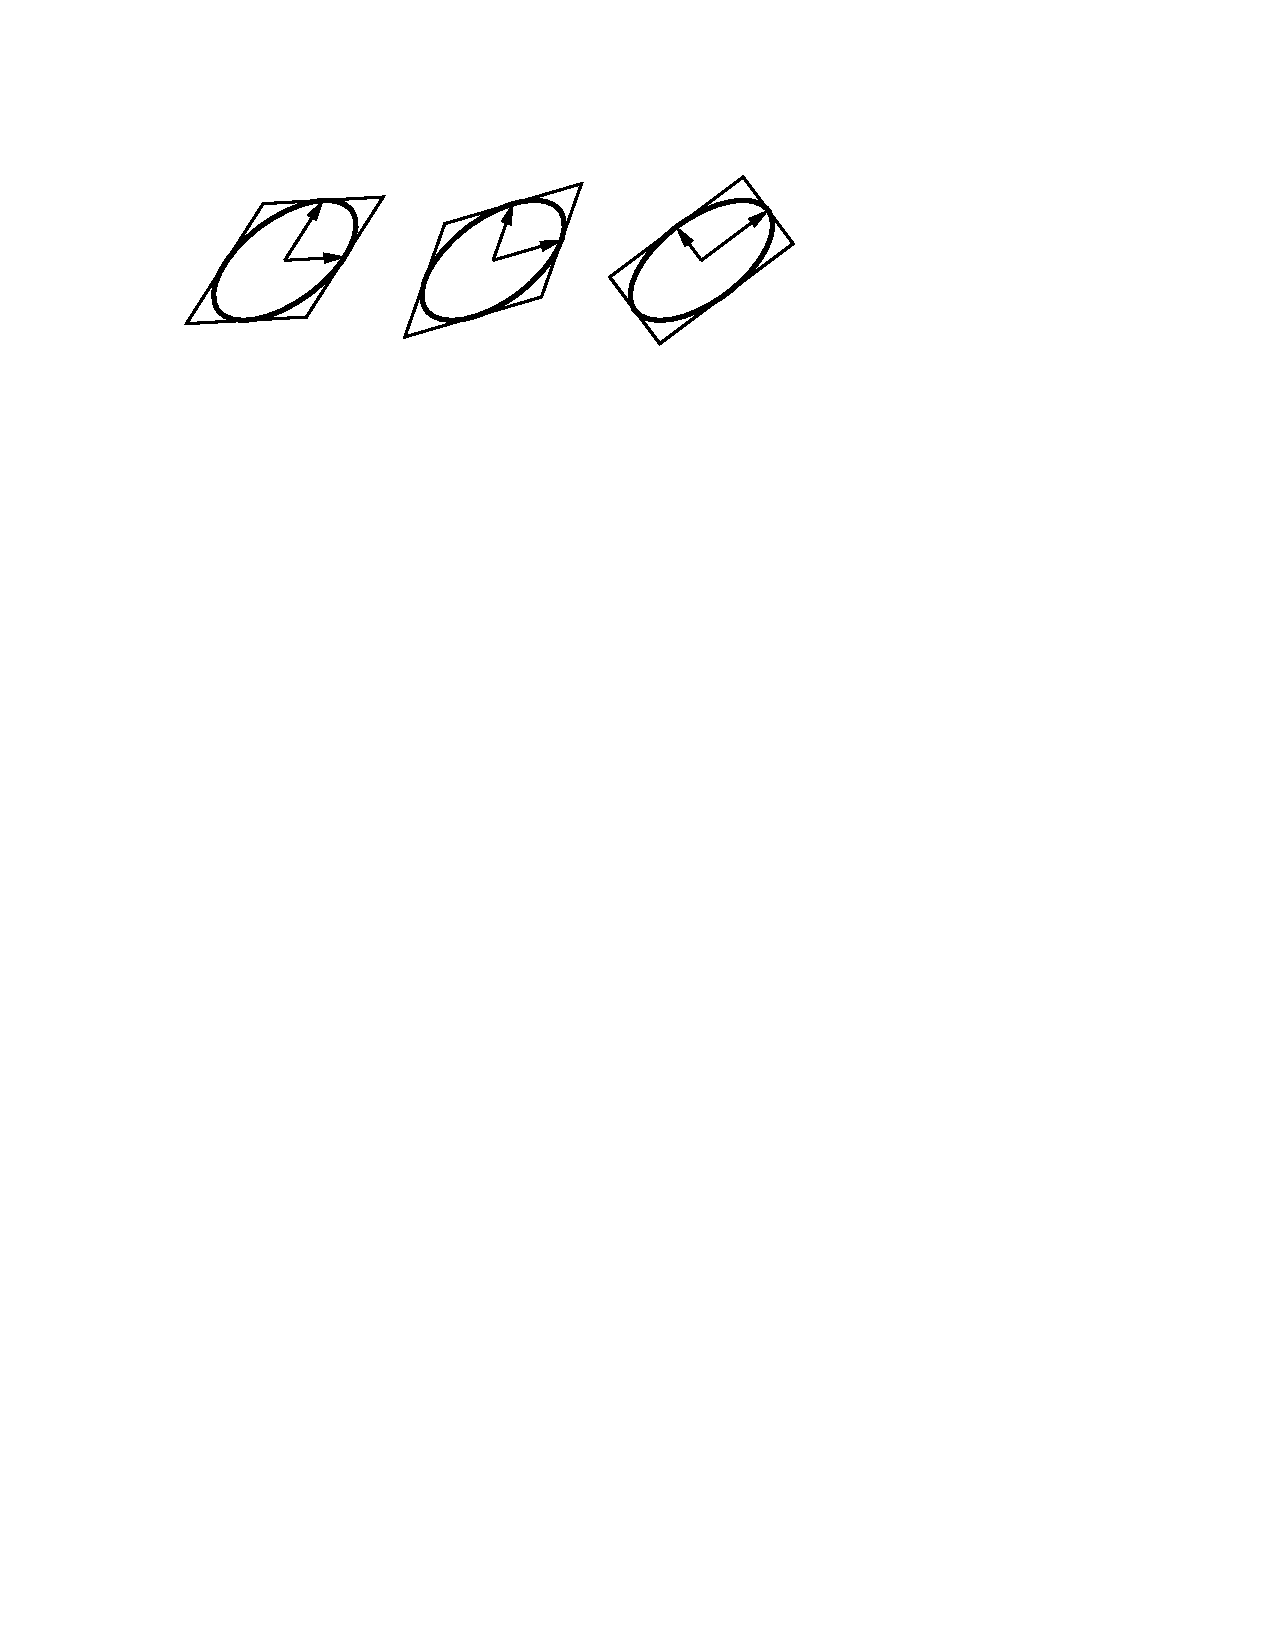
\includegraphics{different-ellipses}}
\caption{Different vectors may specify the same ellipse.}
\end{figure}

The special case of an ellipse with its axes aligned with the coordinate axes
can be obtained by setting $dx_2 = dy_1 = 0$ or $dx_1 = dy_2 = 0$.


\Defprotoclass {ellipse}

The protocol class that corresponds to a mathematical ellipse.  This is a
subclass of \cl{area}.
\IfYouWantClass {an} {ellipse} {ellipse}

\Defpredicate {ellipsep} {object}

Returns \term{true} if \arg{object} is an \term{ellipse}, otherwise returns
\term{false}.

\Defclass {standard-ellipse}

An instantiable class that implements an ellipse.  This is a subclass of
\cl{ellipse}.  This is the class that \cl{make-ellipse} and \cl{make-ellipse*}
instantiate.
\Immutable

\defun {make-ellipse}  {center-point 
                        radius-1-dx radius-1-dy radius-2-dx radius-2-dy
                        \key start-angle end-angle}
\Defun {make-ellipse*} {center-x center-y 
                        radius-1-dx radius-1-dy radius-2-dx radius-2-dy 
                        \key start-angle end-angle}

Returns an object of class \cl{standard-ellipse}.  The center of the ellipse is
at the \term{point} \arg{center-point} (or the position
(\arg{center-x},\arg{center-y})).

Two vectors, (\arg{radius-1-dx},\arg{radius-1-dy}) and
(\arg{radius-2-dx},\arg{radius-2-dy}) specify the bounding parallelogram of the
ellipse as explained above.  All of the radii are real numbers.  If the two
vectors are collinear, the ellipse is not well-defined and the
\cl{ellipse-not-well-defined} error will be signalled.  The special case of an
ellipse with its axes aligned with the coordinate axes can be obtained by
setting both \arg{radius-1-dy} and \arg{radius-2-dx} to 0.

If \arg{start-angle} or \arg{end-angle} are supplied, the ellipse is the ``pie
slice'' area swept out by a line from the center of the ellipse to a point on
the boundary as the boundary point moves from the angle \arg{start-angle} to
\arg{end-angle}.  Angles are measured counter-clockwise with respect to the
positive $x$ axis.  If \arg{end-angle} is supplied, the default for
\arg{start-angle} is $0$; if \arg{start-angle} is supplied, the default for
\arg{end-angle} is $2\pi$; if neither is supplied then the region is a full
ellipse and the angles are meaningless.

\MayCaptureInputs


\Defprotoclass {elliptical-arc}

The protocol class that corresponds to a mathematical elliptical arc.  This is a
subclass of \cl{path}.
\IfYouWantClass {an} {elliptical arc} {elliptical-arc}

\Defpredicate {elliptical-arc-p} {object}

Returns \term{true} if \arg{object} is an \term{elliptical arc}, otherwise
returns \term{false}.

\Defclass {standard-elliptical-arc}

An instantiable class that implements an elliptical arc.  This is a subclass of
\cl{elliptical-arc}.  This is the class that \cl{make-elliptical-arc} and
\cl{make-elliptical-arc*} instantiate.
\Immutable

\defun {make-elliptical-arc}  {center-point
                               radius-1-dx radius-1-dy radius-2-dx radius-2-dy
                               \key start-angle end-angle}
\Defun {make-elliptical-arc*} {center-x center-y 
                               radius-1-dx radius-1-dy radius-2-dx radius-2-dy
                               \key start-angle end-angle}

Returns an object of class \cl{standard-elliptical-arc}.  The center of the
ellipse is at the \term{point} \arg{center-point} (or the position
(\arg{center-x},\arg{center-y})).

Two vectors, (\arg{radius-1-dx},\arg{radius-1-dy}) and
(\arg{radius-2-dx},\arg{radius-2-dy}), specify the bounding parallelogram of the
ellipse as explained above.  All of the radii are real numbers.   If the two
vectors are collinear, the ellipse is not well-defined and the
\cl{ellipse-not-well-defined} error will be signalled.  The special case of
an elliptical arc with its axes aligned with the coordinate axes can be obtained
by setting both \arg{radius-1-dy} and \arg{radius-2-dx} to 0.

If \arg{start-angle} and \arg{end-angle} are supplied, the arc is swept from
\arg{start-angle} to \arg{end-angle}.  Angles are measured counter-clockwise
with respect to the positive $x$ axis.  If \arg{end-angle} is supplied, the
default for \arg{start-angle} is $0$; if \arg{start-angle} is supplied, the
default for \arg{end-angle} is $2\pi$; if neither is supplied then the region is
a closed elliptical path and the angles are meaningless.

\MayCaptureInputs


\subsubsection {The Ellipse and Elliptical Arc Protocol}

The following functions apply to both ellipses and elliptical arcs.  In all
cases, the name \arg{elliptical-object} means that the argument may be an
\term{ellipse} or an \term{elliptical arc}.  These generic functions comprise
the ellipse protocol.  All classes that are subclasses of either \cl{ellipse} or
\cl{elliptical-arc} must implement methods for these functions.

\Defgeneric {ellipse-center-point*} {elliptical-object}

Returns the center point of \arg{elliptical-object} as two values representing
the coordinate pair.

\Defgeneric {ellipse-center-point} {elliptical-object}

Returns the center point of \arg{elliptical-object}.  

\cl{ellipse-center-point} is part of the ellipse API, but not part of the ellipse
protocol.  CLIM will supply default methods for \cl{ellipse-center-point} on the
protocol classes \cl{ellipse} and \cl{elliptical-arc} that are implemented by
calling \cl{ellipse-center-point*}.

\Defgeneric {ellipse-radii} {elliptical-object}

Returns four values corresponding to the two radius vectors of
\arg{elliptical-arc}.  These values may be canonicalized in some way, and so may
not be the same as the values passed to the constructor function.

\Defgeneric {ellipse-start-angle} {elliptical-object}

Returns the start angle of \arg{elliptical-object}.  If \arg{elliptical-object}
is a full ellipse or closed path then \cl{ellipse-start-angle} will return
\cl{nil}; otherwise the value will be a number greater than or equal to zero,
and less than $2\pi$.

\Defgeneric {ellipse-end-angle} {elliptical-object}

Returns the end angle of \arg{elliptical-object}.  If \arg{elliptical-object} is
a full ellipse or closed path then \cl{ellipse-end-angle} will return \cl{nil};
otherwise the value will be a number greater than zero, and less than or equal
to $2\pi$.


% -*- Mode: LaTeX; Package: CLIM-USER -*-

\chapter {Bounding Rectangles}
\label {bboxes}

\section {Bounding Rectangles}

Every bounded region has a derived \concept{bounding rectangle}, which is a
rectangular region whose sides are parallel to the coordinate axes.  Therefore,
every bounded region participates in the bounding rectangle protocol.  The
bounding rectangle for a region is the smallest rectangle that contains every
point in the region.  However, the bounding rectangle may contain additional
points as well.  Unbounded regions do not have a bounding rectangle and do not
participate in the bounding rectangle protocol.  Other objects besides bounded
regions participate in the bounding rectangle protocol, such as sheets and
output records.

The coordinate system in which the bounding rectangle is maintained depends on
the context.  For example, the coordinates of the bounding rectangle of a sheet
are expressed in the sheet's parent's coordinate system.  For output records,
the coordinates of the bounding rectangle are maintained in the coordinate
system of the stream with which the output record is associated.

Note that the bounding rectangle of a transformed region is not in general the
same as the result of transforming the bounding rectangle of a region, as shown
in Figure~\ref{output-record-bbox}.  For transformations that satisfy
\cl{rectilinear-transformation-p}, the following equality holds.  For all other
transformations, it does not hold.

\begin{verbatim}
(region-equal
  (transform-region transformation (bounding-rectangle region))
  (bounding-rectangle (transform-region transformation region)))
\end{verbatim}

\begin{figure}
\centerline{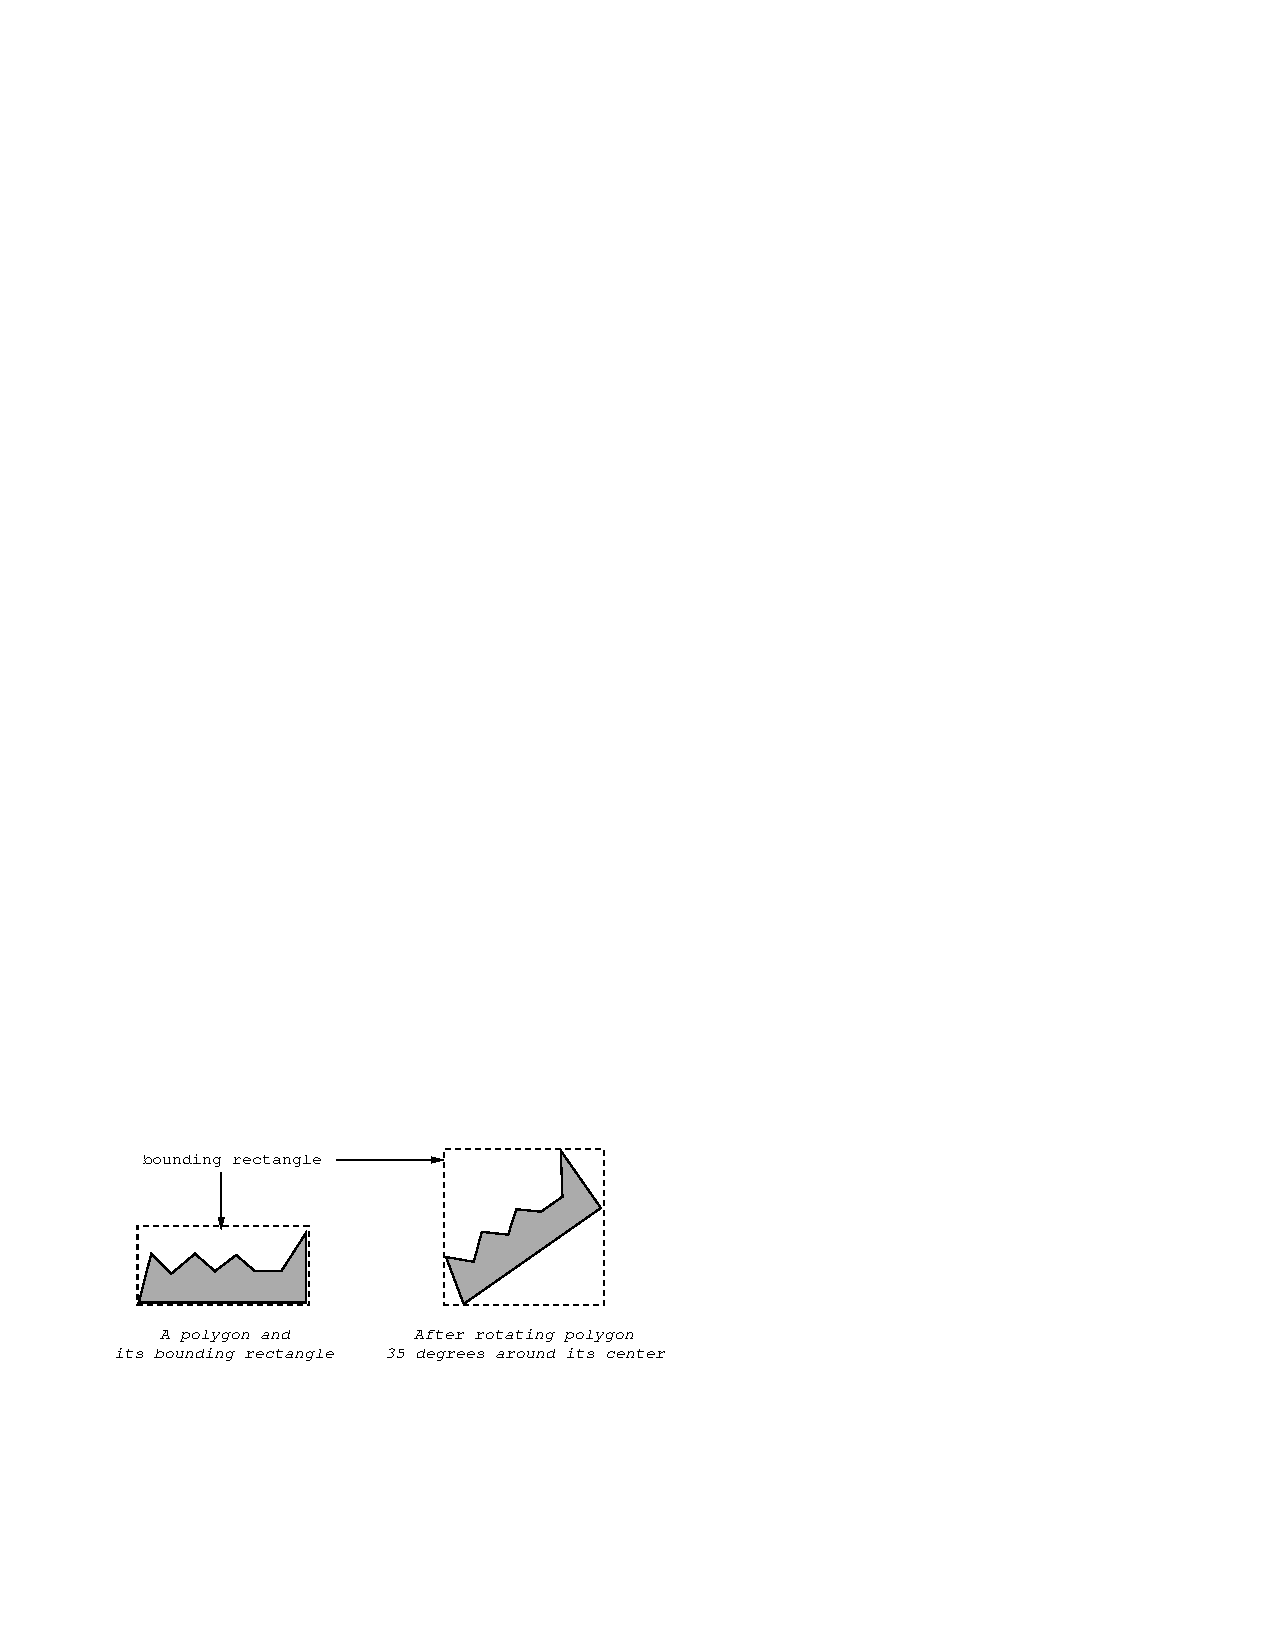
\epsfig{file=bounding-box.epsi}}
\caption{\label{output-record-bbox} The bounding rectangle of an output record.}
\end{figure}

CLIM uses bounding rectangles for a variety of purposes.  For example,
repainting of windows is driven from the bounding rectangle of the window's
viewport, intersected with a ``damage'' region.  The formatting engines used by
\cl{formatting-table} and \cl{formatting-graph} operate on the bounding
rectangles of the output records in the output.  Bounding rectangles are also
used internally by CLIM to achieve greater efficiency.  For instance, when
performing hit detection to see if the pointer is within the region of an output
record, CLIM first checks to see if the pointer is within the bounding rectangle
of the output record.

Note that the bounding rectangle for an output record may have a different size
depending on the medium on which the output record is rendered.  Consider the
case of rendering text on different output devices; the font chosen for a
particular text style may vary considerably in size from one device to another.

\Defprotoclass {bounding-rectangle}

The protocol class that represents a bounding rectangle.
\IfYouWantClass {a} {bounding rectangle} {bounding-rectangle}

Note that bounding rectangles are not a subclass of \cl{rectangle}, nor even a
subclass of \cl{region}.  This is because, in general, bounding rectangles do
not obey the region protocols.  However, all bounded regions and sheets that
obey the bounding rectangle protocol are subclasses of \cl{bounding-rectangle}.

Bounding rectangles are immutable, but since they reflect the live state of such
mutable objects as sheets and output records, bounding rectangles are volatile.
Therefore, programmers must not depend on the bounding rectangle associated with
a mutable object remaining constant.

\Defpredicate {bounding-rectangle-p} {object}

Returns \term{true} if \arg{object} is a \term{bounding rectangle} (that is,
supports the bounding rectangle protocol), otherwise returns \term{false}.

\Defclass {standard-bounding-rectangle}

An instantiable class that implements a bounding rectangle.  This is a subclass
of both \cl{bounding-rectangle} and \cl{rectangle}, that is, standard bounding
rectangles obey the rectangle protocol.

\cl{make-bounding-rectangle} returns an object of this class.

The representation of bounding rectangles in CLIM is chosen to be efficient.
CLIM will probably represent such rectangles by storing the coordinates of two
opposing corners of the rectangle, namely, the ``min point'' and the ``max
point''.  Because this representation is not sufficient to represent the result
of arbitrary transformations of arbitrary rectangles, CLIM is allowed to return
a polygon as the result of such a transformation.  (The most general class of
transformations that is guaranteed to always turn a rectangle into another
rectangle is the class of transformations that satisfy
\cl{rectilinear-transformation-p}.)

\Defun {make-bounding-rectangle} {x1 y1 x2 y2}

Returns an object of the class \cl{standard-bounding-rectangle} with the edges
specified by \arg{x1}, \arg{y1}, \arg{x2}, and \arg{y2}, which must be real
numbers.

\arg{x1}, \arg{y1}, \arg{x2}, and \arg{y2} are ``canonicalized'' in the
following way.  The min point of the rectangle has an $x$ coordinate that is the
smaller of \arg{x1} and \arg{x2} and a $y$ coordinate that is the smaller of
\arg{y1} and \arg{y2}.  The max point of the rectangle has an $x$ coordinate
that is the larger of \arg{x1} and \arg{x2} and a $y$ coordinate that is the
larger of \arg{y1} and \arg{y2}.  (Therefore, in a right-handed coordinate
system the canonicalized values of \arg{x1}, \arg{y1}, \arg{x2}, and \arg{y2}
correspond to the left, top, right, and bottom edges of the rectangle,
respectively.)

\FreshOutputs


\subsection {The Bounding Rectangle Protocol}

The following generic function comprises the bounding rectangle protocol.  All
classes that participate in this protocol (including all subclasses of
\cl{region} that are bounded regions) must implement a method for
\cl{bounding-rectangle*}.

\Defgeneric {bounding-rectangle*} {region}

Returns the bounding rectangle of \arg{region} as four real numbers specifying
the $x$ and $y$ coordinates of the min point and the $x$ and $y$ coordinates of
the max point of the rectangle.  The argument \arg{region} must be either a
bounded region (such as a line or an ellipse) or some other object that obeys
the bounding rectangle protocol, such as a sheet or an output record.

The four returned values \arg{min-x}, \arg{min-y}, \arg{max-x}, and \arg{max-y}
will satisfy the inequalities
\begin{eqnarray*}
  minx \leq maxx \\
  miny \leq maxy \\
\end{eqnarray*}


\Defgeneric {bounding-rectangle} {region}

Returns the bounding rectangle of \arg{region} as an object that is a subclass
of \cl{rectangle} (described in Section~\ref{rect}).  The argument \arg{region}
must be either a bounded region (such as a line or an ellipse) or some other
object that obeys the bounding rectangle protocol, such as a sheet or an output
record.

It is unspecified whether \cl{bounding-rectangle} will or will not create a new
object each time it is called.  Many CLIM implementations will cache the
bounding rectangle for sheets and output records.  The implication of this is
that, since bounding rectangles are volatile, programmers should depend on the
object returned by \cl{bounding-rectangle} remaining constant.

\cl{bounding-rectangle} is part of the bounding rectangle API, but not part of
the bounding rectangle protocol.  CLIM will supply a default method for
\cl{bounding-rectangle} on the protocol class \cl{bounding-rectangle} that is
implemented by calling \cl{bounding-rectangle*}.


\subsection {Bounding Rectangle Convenience Functions}

The functions described below are part of the bounding rectangle API, but are
not part of the bounding rectangle protocol.  They are provided as a convenience
to programmers who wish to specialize classes that participate in the bounding
rectangle protocol, but do not complicate the task of those programmers who
define their own types (such as sheet classes) that participate in this
protocol.

CLIM will supply default methods for all of these generic functions on the
protocol class \cl{bounding-rectangle} that are implemented by calling
\cl{bounding-rectangle*}.


\Defmacro {with-bounding-rectangle*} {(min-x min-y max-x max-y) region \body body}  

Binds \arg{min-x}, \arg{min-y}, \arg{max-x}, and \arg{max-y} to the edges of the
bounding rectangle of \arg{region}, and then executes \arg{body} in that
context.  The argument \arg{region} must be either a bounded region (such as a
line or an ellipse) or some other object that obeys the bounding rectangle
protocol, such as a sheet or an output record.

The arguments \arg{min-x}, \arg{min-y}, \arg{max-x}, and \arg{max-y} are not
evaluated.  \arg{body} may have zero or more declarations as its first forms.

\cl{with-bounding-rectangle*} must be implemented by calling \cl{bounding-rectangle*}.


\Defgeneric {bounding-rectangle-position} {region}

Returns the position of the bounding rectangle of \arg{region}.  The position of
a bounding rectangle is specified by its min point.


\defgeneric {bounding-rectangle-min-x} {region}
\defgeneric {bounding-rectangle-min-y} {region}
\defgeneric {bounding-rectangle-max-x} {region}
\Defgeneric {bounding-rectangle-max-y} {region}

Returns (respectively) the $x$ and $y$ coordinates of the min point and the $x$
and $y$ coordinate of the max point of the bounding rectangle of \arg{region}.
The argument \arg{region} must be either a bounded region or some other object
that obeys the bounding rectangle protocol.


\defgeneric {bounding-rectangle-width}  {region}
\defgeneric {bounding-rectangle-height} {region}
\Defgeneric {bounding-rectangle-size}   {region}

Returns the width, height, or size (as two values, the width and height) of the
bounding rectangle of \arg{region}, respectively.  The argument \arg{region}
must be either a bounded region or some other object that obeys the bounding
rectangle protocol.

The width of a bounding rectangle is the difference between its maximum $x$
coordinate and its minimum $x$ coordinate.  The height is the difference between
the maximum $y$ coordinate and its minimum $y$ coordinate.

% -*- Mode: LaTeX; Package: CLIM-USER -*-

\chapter {Affine Transformations}
\label {transforms}

An \concept{affine transformation} is a mapping from one coordinate system onto
another that preserves straight lines.  In other words, if you take a number of
points that fall on a straight line and apply an affine transformation to their
coordinates, the transformed coordinates will describe a straight line in the
new coordinate system.  General affine transformations include all the sorts of
transformations that CLIM uses, namely, translations, scaling, rotations, and
reflections.


\section {Transformations}

\Defprotoclass {transformation}

The protocol class of all transformations.  There are one or more subclasses of
\cl{transformation} with implementation-dependent names that implement
transformations.  The exact names of these classes is explicitly unspecified.
\IfYouWantClass {a} {transformation} {transformation}

All of the instantiable transformation classes provided by CLIM are immutable.

\Defpredicate {transformationp} {object}

Returns \term{true} if \arg{object} is a \term{transformation}, otherwise
returns \term{false}.

\Defconst {+identity-transformation+}

An instance of a transformation that is guaranteed to be an identity
transformation, that is, the transformation that ``does nothing''.


\subsection {Transformation Conditions}

\Deferror {transformation-error}

The class that is the superclass of the following three conditions.  This class
is a subclass of \cl{error}.

\Deferror {transformation-underspecified}

The error that is signalled when \cl{make-3-point-transformation} is given three
collinear image points.  This condition will handle the \cl{:points} initarg,
which is used to supply the points that are in error.

\Deferror {reflection-underspecified}

The error that is signalled when \cl{make-reflection-transformation} is given
two coincident points.  This condition will handle the \cl{:points} initarg,
which is used to supply the points that are in error.

\Deferror {singular-transformation}

The error that is signalled when \cl{invert-transformation} is called on a
singular transformation, that is, a transformation that has no inverse.  This
condition will handle the \cl{:transformation} initarg, which is used to supply
the transformation that is singular.


\section {Transformation Constructors}

The following transformation constructors do not capture any of their inputs.
The constructors all create objects that are subclasses of \cl{transformation}.

\Defun {make-translation-transformation} {translation-x translation-y} 

A translation is a transformation that preserves length, angle, and orientation
of all geometric entities.

\cl{make-translation-transformation} returns a transformation that translates
all points by \arg{translation-x} in the $x$ direction and \arg{translation-y}
in the $y$ direction.  \arg{translation-x} and \arg{translation-y} must be real
numbers.


\defun {make-rotation-transformation}  {angle \optional origin}
\Defun {make-rotation-transformation*} {angle \optional origin-x origin-y}

A rotation is a transformation that preserves length and angles of all geometric
entities.  Rotations also preserve one point (the origin) and the distance of
all entities from that point.

\cl{make-rotation-transformation} returns a transformation that rotates all
points by \arg{angle} (which is a real number indicating an angle in radians)
around the point \arg{origin}.  If \arg{origin} is supplied it must be a point;
if not supplied it defaults to $(0,0)$.  \arg{origin-x} and \arg{origin-y} must
be real numbers, and default to $0$.

\defun {make-scaling-transformation}  {scale-x scale-y \optional origin} 
\Defun {make-scaling-transformation*} {scale-x scale-y \optional origin-x origin-y} 

There is no single definition of a scaling transformation.  Transformations that
preserve all angles and multiply all lengths by the same factor (preserving the
``shape'' of all entities) are certainly scaling transformations.  However,
scaling is also used to refer to transformations that scale distances in the $x$
direction by one amount and distances in the $y$ direction by another amount.

\cl{make-scaling-transformation} returns a transformation that multiplies the
$x$-coordinate distance of every point from \arg{origin} by \arg{scale-x} and
the $y$-coordinate distance of every point from \arg{origin} by \arg{scale-y}.
\arg{scale-x} and \arg{scale-y} must be real numbers.  If \arg{origin} is
supplied it must be a point; if not supplied it defaults to $(0,0)$.
\arg{origin-x} and \arg{origin-y} must be real numbers, and default to $0$.


\defun {make-reflection-transformation}  {point1 point2}
\Defun {make-reflection-transformation*} {x1 y1 x2 y2}

A reflection is a transformation that preserves lengths and magnitudes of
angles, but changes the sign (or ``handedness'') of angles.  If you think of the
drawing plane on a transparent sheet of paper, a reflection is a transformation
that ``turns the paper over''.

\cl{make-reflection-transformation} returns a transformation that reflects every
point through the line passing through the \term{points} \arg{point1} and
\arg{point2} (or through the positions $(x1,y1)$ and $(x2,y2)$ in the case of
the spread version).


\Defun {make-transformation} {mxx mxy myx myy tx ty}

Returns a general transformation whose effect is:
\begin{eqnarray*}
  x^\prime =& m_{xx} x + m_{xy} y + t_x \\
  y^\prime =& m_{yx} x + m_{yy} y + t_y
\end{eqnarray*}
where $x$ and $y$ are the coordinates of a point before the transformation and
$x^\prime$ and $y^\prime$ are the coordinates of the corresponding point after.

All of the arguments to \cl{make-transformation} must be real numbers.


\Defun {make-3-point-transformation} {point-1 point-2 point-3 point-1-image point-2-image point-3-image}

Returns a transformation that takes \term{points} \arg{point-1} into
\arg{point-1-image}, \arg{point-2} into \arg{point-2-image} and \arg{point-3}
into \arg{point-3-image}.  Three non-collinear points and their images under the
transformation are enough to specify any affine transformation.

If \arg{point-1}, \arg{point-2} and \arg{point-3} are collinear, the
\cl{transformation-underspecified} error will be signalled.  If
\arg{point-1-image}, \arg{point-2-image} and \arg{point-3-image} are collinear,
the resulting transformation will be singular (that is, will have no inverse)
but this is not an error.


\Defun {make-3-point-transformation*} {x1 y1 x2 y2 x3 y3 x1-image y1-image x2-image y2-image x3-image y3-image}

Returns a transformation that takes the points at the positions
(\arg{x1},\arg{y1}) into (\arg{x1-image},\arg{y1-image}), (\arg{x2},\arg{y2})
into (\arg{x2-image},\arg{y2-image}) and (\arg{x3},\arg{y3}) into
(\arg{x3-image},\arg{y3-image}).  Three non-collinear points and their images
under the transformation are enough to specify any affine transformation.

If the positions $(x1,y1)$, $(x2,y2)$ and $(x3,y3)$ are collinear, the
\cl{transformation-underspecified} error will be signalled.  If
(\arg{x1-image},\arg{y1-image}), (\arg{x2-image},\arg{y2-image}), and
(\arg{x3-image},\arg{y3-image}) are collinear, the resulting transformation will
be singular but this is not an error.

This is the spread version of \cl{make-3-point-transformation}.


\section {The Transformation Protocol}

The following subsections describe the transformation protocol.  All classes
that are subclasses of \cl{transformation} must implement methods for all of
the generic functions in the following subsections.


\subsection {Transformation Predicates}

In all of the functions below, the argument named \arg{transformation} must be a
transformation.

\Defgeneric {transformation-equal} {transformation1 transformation2} 

Returns \term{true} if the two \term{transformations} \arg{transformation1} and
\arg{transformation2} have equivalent effects (that is, are mathematically
equal), otherwise returns \term{false}.

Implementations are encouraged to allow transformations that are not numerically
equal due to floating-point roundoff errors to be \cl{transformation-equal}.  An
appropriate level of ``fuzziness'' is \cl{single-float-epsilon}, or some small
multiple of \cl{single-float-epsilon}.


\Defgeneric {identity-transformation-p} {transformation} 

Returns \term{true} if the \term{transformation} \arg{transformation} is equal
(in the sense of \cl{transformation-equal}) to the identity transformation,
otherwise returns \term{false}.

\Defgeneric {invertible-transformation-p} {transformation} 

Returns \term{true} if the \term{transformation} \arg{transformation} has an
inverse, otherwise returns \term{false}.

\Defgeneric {translation-transformation-p} {transformation}

Returns \term{true} if the \term{transformation} \arg{transformation} is a pure
translation, that is, a transformation such that there are two distance
components $dx$ and $dy$ and every point $(x,y)$ is moved to $(x+dx,y+dy)$.
Otherwise, \cl{translation-transformation-p} returns \term{false}.

\Defgeneric {reflection-transformation-p} {transformation}

Returns \term{true} if the \term{transformation} \arg{transformation} inverts
the ``handedness'' of the coordinate system, otherwise returns \term{false}.
Note that this is a very inclusive category---transformations are considered
reflections even if they distort, scale, or skew the coordinate system, as long
as they invert the handedness.

\Defgeneric {rigid-transformation-p} {transformation}

Returns \term{true} if the \term{transformation} \arg{transformation} transforms
the coordinate system as a rigid object, that is, as a combination of
translations, rotations, and pure reflections.  Otherwise, it returns
\term{false}.

Rigid transformations are the most general category of transformations that
preserve magnitudes of all lengths and angles.

\Defgeneric {even-scaling-transformation-p} {transformation}

Returns \term{true} if the \term{transformation} \arg{transformation} multiplies
all $x$ lengths and $y$ lengths by the same magnitude, otherwise returns
\term{false}.  It does include pure reflections through vertical and horizontal
lines.

\Defgeneric {scaling-transformation-p} {transformation}

Returns \term{true} if the \term{transformation} \arg{transformation} multiplies
all $x$ lengths by one magnitude and all $y$ lengths by another magnitude,
otherwise returns \term{false}.  This category includes even scalings as a
subset.

\Defgeneric {rectilinear-transformation-p} {transformation}

Returns \term{true} if the \term{transformation} \arg{transformation} will
always transform any axis-aligned rectangle into another axis-aligned rectangle,
otherwise returns \term{false}.  This category includes scalings as a subset,
and also includes 90 degree rotations.

Rectilinear transformations are the most general category of transformations for
which the bounding rectangle of a transformed object can be found by
transforming the bounding rectangle of the original object.

\issue {SWM} {Supply this figure.}

\begin{figure}
\centerline{To be supplied.}
\caption{The predicates for analyzing the mathematical properties of a transformation.}  
\end{figure}


\subsection {Composition of Transformations}

If we transform from one coordinate system to another, then from the second to a
third coordinate system, we can regard the resulting transformation as a single
transformation resulting from \concept{composing} the two component
transformations.  It is an important and useful property of affine transformations
that they are closed under composition.  Note that composition is not commutative;
in general, the result of applying transformation $A$ and then applying
transformation $B$ is not the same as applying $B$ first, then $A$.

Any arbitrary transformation can be built up by composing a number of simpler
transformations, but that composition is not unique.

\Defgeneric {compose-transformations} {transformation1 transformation2}

Returns a transformation that is the mathematical composition of its arguments.
Composition is in right-to-left order, that is, the resulting transformation
represents the effects of applying the \term{transformation}
\arg{transformation2} followed by the \term{transformation}
\arg{transformation1}.

\Defgeneric {invert-transformation} {transformation}

Returns a transformation that is the inverse of the \term{transformation}
\arg{transformation}.  The result of composing a transformation with its inverse
is equal to the identity transformation.

If \arg{transformation} is singular, \cl{invert-transformation} will signal the
\cl{singular-transformation} error, with a named restart that is invoked with a
transformation and makes \cl{invert-transformation} return that transformation.
This is to allow a drawing application, for example, to use a generalized
inverse to transform a region through a singular transformation.

Note that with finite-precision arithmetic there are several low-level
conditions that might occur during the attempt to invert a singular or ``almost
singular'' transformation.  (These include computation of a zero determinant,
floating-point underflow during computation of the determinant, or
floating-point overflow during subsequent multiplication.)
\cl{invert-transformation} must signal the \cl{singular-transformation} error
for all of these cases.

\defun {compose-translation-with-transformation} {transformation dx dy}
\defun {compose-scaling-with-transformation}     {transformation sx sy \optional origin}
\Defun {compose-rotation-with-transformation}    {transformation angle \optional origin} 

These functions create a new transformation by composing the
\term{transformation} \arg{transformation} with a given translation, scaling, or
rotation, respectively.  The order of composition is that the translation,
scaling, or rotation ``transformation'' is first, followed by
\arg{transformation}.

\arg{dx} and \arg{dy} are as for \cl{make-translation-transformation}.
\arg{sx} and \arg{sy} are as for \cl{make-scaling-transformation}.
\arg{angle} and \arg{origin} are as for \cl{make-rotation-transformation}.

Note that these functions could be implemented by using the various constructors
and \cl{compose-transformations}.  They are provided, because it is common to
build up a transformation as a series of simple transformations.


\defun {compose-transformation-with-translation} {transformation dx dy}
\defun {compose-transformation-with-scaling}     {transformation sx sy \optional origin}
\Defun {compose-transformation-with-rotation}    {transformation angle \optional origin} 

These functions create a new transformation by composing a given translation,
scaling, or rotation, respectively, with the \term{transformation}
\arg{transformation}.  The order of composition is \arg{transformation} is
first, followed by the translation, scaling, or rotation ``transformation''.

\arg{dx} and \arg{dy} are as for \cl{make-translation-transformation}.
\arg{sx} and \arg{sy} are as for \cl{make-scaling-transformation}.
\arg{angle} and \arg{origin} are as for \cl{make-rotation-transformation}.

Note that these functions could be implemented by using the various constructors
and \cl{compose-transformations}.  They are provided, because it is common to
build up a transformation as a series of simple transformations.


\subsection {Applying Transformations}

Transforming a region applies a coordinate transformation to that region, thus
moving its position on the drawing plane, rotating it, or scaling it.  Note that
transforming a region does not side-effect the \arg{region} argument; it is free
to either create a new region or return an existing (cached) region.

These generic functions must be implemented for all classes of transformations.
Furthermore, all subclasses of \cl{region} and \cl{design} must implement
methods for \cl{transform-region} and \cl{untransform-region}.  That is, methods
for the following generic functions will typically specialize both the
\arg{transformation} and \term{region} arguments.

Note that, if the extended region classes are not implemented, the following
functions are not closed, that is, they may return results that are not CLIM
regions.


\Defgeneric {transform-region} {transformation region}

Applies \arg{transformation} to the \term{region} \arg{region}, and returns the
transformed region.

\Defgeneric {untransform-region} {transformation region}

This is exactly equivalent to \\
\verb+(transform-region (invert-transformation+ \arg{transformation}\verb+)+
\arg{region}\verb+)+ .

CLIM provides a default method for \cl{untransform-region} on the
\cl{transformation} protocol class that does exactly this.


\Defgeneric {transform-position} {transformation x y}

Applies the \term{transformation} \arg{transformation} to the point whose
coordinates are the real numbers \arg{x} and \arg{y}, and returns two values,
the transformed $x$ coordinate and the transformed $y$ coordinate.

\cl{transform-position} is the spread version of \cl{transform-region} in the
case where the region is a point.

\Defgeneric {untransform-position} {transformation x y}

This is exactly equivalent to \\
\verb+(transform-position (invert-transformation+ \arg{transformation}\verb+)+
\arg{x} \arg{y}\verb+)+ .

CLIM provides a default method for \cl{untransform-position} on the
\cl{transformation} protocol class that does exactly this.


\Defgeneric {transform-distance} {transformation dx dy}

Applies the \term{transformation} \arg{transformation} to the distance
represented by the real numbers \arg{dx} and \arg{dy}, and returns two values,
the transformed \arg{dx} and the transformed \arg{dy}.

A distance represents the difference between two points.  It does {\sl not}
transform like a point.

\Defgeneric {untransform-distance} {transformation dx dy} 

This is exactly equivalent to \\
\verb+(transform-distance (invert-transformation+ \arg{transformation}\verb+)+
\arg{dx} \arg{dy}\verb+)+ .

CLIM provides a default method for \cl{untransform-distance} on the
\cl{transformation} protocol class that does exactly this.


\Defgeneric {transform-rectangle*} {transformation x1 y1 x2 y2}

Applies the \term{transformation} \arg{transformation} to the rectangle
specified by the four coordinate arguments, which are real numbers.  The
arguments \arg{x1}, \arg{y1}, \arg{x2}, and \arg{y1} are canonicalized in the
same way as for \cl{make-bounding-rectangle}.  Returns four values that specify
the minimum and maximum points of the transformed rectangle in the order
\arg{min-x}, \arg{min-y}, \arg{max-x}, and \arg{max-y}.

It is an error is \arg{transformation} does not satisfy
\cl{rectilinear-transformation-p}.

\cl{transform-rectangle*} is the spread version of \cl{transform-region} in the
case where the transformation is rectilinear and the region is a rectangle.

\Defgeneric {untransform-rectangle*} {transformation x1 y1 x2 y2}

This is exactly equivalent to \\
\verb+(transform-rectangle* (invert-transformation+ \arg{transformation}\verb+)+
\arg{x1} \arg{y1} \arg{x2} \arg{y2}\verb+)+ .

CLIM provides a default method for \cl{untransform-rectangle*} on the
\cl{transformation} protocol class that does exactly this.


\part{Windowing Substrate}
% -*- Mode: LaTeX; Package: CLIM-USER -*-

\chapter {Overview of Window Facilities}

\section {Introduction}

A central notion in organizing user interfaces is allocating screen regions to
particular tasks and recursively subdividing these regions into subregions.  The
windowing layer of CLIM defines an extensible framework for constructing, using,
and managing such \concept{hierarchies of interactive regions}.  This framework
allows uniform treatment of the following things:

\begin{itemize}
\item Window objects like those in X or NeWS.

\item Lightweight gadgets typical of toolkit layers, such as Motif or OpenLook.

\item Structured graphics like output records and an application's presentation
objects.

\item Objects that act as Lisp handles for windows or gadgets implemented in a
different language (such as OpenLook gadgets implemented in C).
\end{itemize}

From the perspective of most CLIM users, CLIM's windowing layer plays the role
of a window system.  However, CLIM will usually use the services of a window
system platform to provide efficient windowing, input, and output facilities.
In this specification, such window system platforms will be referred to as host
window systems or as display servers.

The fundamental window abstraction defined by CLIM is called a \concept{sheet}.
A sheet can participate in a relationship called a \concept{windowing
relationship}.  This relationship is one in which one sheet called the
\concept{parent} provides space to a number of other sheets called
\concept{children}.  Support for establishing and maintaining this kind of
relationship is the essence of what window systems provide.  At any point in
time, CLIM allows a sheet to be a child in one relationship called its
\concept{youth windowing relationship} and a parent in another relationship
called its \concept{adult windowing relationship}.

Programmers can manipulate unrooted hierarchies of sheets (those without a
connection to any particular display server).  However, a sheet hierarchy must
be attached to a display server to make it visible.  \concept{Ports} and
\concept{grafts} provide the functionality for managing this capability.  A
\term{port} is an abstract connection to a display service that is responsible
for managing host display server resources and for processing input events
received from the host display server.  A \term{graft} is a special kind of
sheet that represents a host window, typically a root window (that is, a
screen-level window).  A sheet is attached to a display by making it a child of
a graft, which represents an appropriate host window.  The sheet will then
appear to be a child of that host window.  So, a sheet is put onto a particular
screen by making it a child of an appropriate graft and enabling it.  Ports and
grafts are described in detail in Chapter~\ref{ports-and-grafts}.


\section {Properties of Sheets}

Sheets have the following properties:

\begin{description}
\item [A coordinate system] Provides the ability to refer to locations in a
sheet's abstract plane.

\item [A region] Defines an area within a sheet's coordinate system that
indicates the area of interest within the plane, that is, a clipping region for
output and input.  This typically corresponds to the visible region of the sheet
on the display.

\item [A parent] A sheet that is the parent in a windowing relationship in which
this sheet is a child.

\item [Children] An ordered set of sheets that are each a child in a windowing
relationship in which this sheet is a parent.  The ordering of the set
corresponds to the stacking order of the sheets.  Not all sheets have children.

\item [A transformation] Determines how points in this sheet's coordinate system
are mapped into points in its parents.

\item [An enabled flag] Indicates whether the sheet is currently actively
participating in the windowing relationship with its parent and siblings.

\item [An event handler] A procedure invoked when the display server wishes to
inform CLIM of external events.

\item [Output state] A set of values used when CLIM causes graphical or textual
output to appear on the display.  This state is often represented by a medium.
\end{description}


\section {Sheet Protocols}

A sheet is a participant in a number of protocols.  Every sheet must provide
methods for the generic functions that make up these protocols.  These protocols
are:

\begin{description}
\item [The windowing protocol] Describes the relationships between the sheet and
its parent and children (and, by extension, all of its ancestors and
descendants).

\item [The input protocol] Provides the event handler for a sheet.  Events may
be handled synchronously, asynchronously, or not at all.

\item [The output protocol] Provides graphical and textual output, and manages
descriptive output state such as color, transformation, and clipping.

\item [The repaint protocol] Invoked by the event handler and by user programs
to ensure that the output appearing on the display device appears as the program
expects it to appear.

\item [The notification protocol] Invoked by the event handler and user programs
to ensure that CLIM's representation of window system information is equivalent
to the display server's.
\end{description}

These protocols may be handled directly by a sheet, queued for later processing
by some other agent, or passed on to a delegate sheet for further processing.


\chapter {Properties of Sheets}
\label {sheet-properties}

\section {Basic Sheet Classes}

Note that there are no standard sheet classes in CLIM, and no pre-packaged way
to create sheets in general.  If a programmer needs to create an instance of
some class of sheet, \cl{make-instance} must be used.  For most purposes,
calling \cl{make-pane} is how application programmers will make sheets.

\Defprotoclass {sheet}

The protocol class that corresponds to a sheet.  This and the next chapter
describe all of the sheet protocols.
\IfYouWantClass {a} {sheet} {sheet}

All of the subclasses of \cl{sheet} are mutable.

\Defpredicate {sheetp} {object}

Returns \term{true} if \arg{object} is a \term{sheet}, otherwise returns
\term{false}.

\Defclass {basic-sheet}

The basic class on which all CLIM sheets are built, a subclass of \cl{sheet}.
\AbstractClass



\section {Relationships Between Sheets}

Sheets are arranged in a tree-structured, acyclic, top-down hierarchy.  Thus, in
general, a sheet has one parent (or no parent) and zero or more children.  A
sheet may have zero or more siblings (that is, other sheets that share the same
parent).  In order to describe the relationships between sheets, we need to
define some terms.

\begin{description}
\item [Adopted] A sheet is said to be \concept{adopted} if it has a parent.  A
sheet becomes the parent of another sheet by adopting that sheet.

\item [Disowned] A sheet is said to be \concept{disowned} if it does not have a
parent.  A sheet ceases to be a child of another sheet by being disowned.

\item [Grafted] A sheet is said to be \concept{grafted} when it is part of a
sheet hierarchy whose highest ancestor is a graft.  In this case, the sheet may
be visible on a particular window server.

\item [Degrafted] A sheet is said to be \concept{degrafted} when it is part of a
sheet hierarchy that cannot possibly be visible on a server, that is, the
highest ancestor is not a graft.

\item [Enabled] A sheet is said to be \concept{enabled} when it is actively
participating in the windowing relationship with its parent.  If a sheet is
enabled and grafted, and all its ancestors are enabled (they are grafted by
definition), then the sheet will be visible if it occupies a portion of the
graft region that isn't clipped by its ancestors or ancestors' siblings.

\item [Disabled] The opposite of enabled is \concept{disabled}.
\end{description}


\subsection {Sheet Relationship Functions}

The generic functions in this section comprise the sheet protocol.  All sheet
objects must implement or inherit methods for each of these generic functions.

\Defgeneric {sheet-parent} {sheet} 

Returns the parent of the \term{sheet} \arg{sheet}, or \cl{nil} if the sheet has
no parent.

\Defgeneric {sheet-children} {sheet}

Returns a list of sheets that are the children of the \term{sheet} \arg{sheet}.
Some sheet classes support only a single child; in this case, the result of
\cl{sheet-children} will be a list of one element.
\ReadOnly

\Defgeneric {sheet-adopt-child} {sheet child}

Adds the child sheet \arg{child} to the set of children of the \term{sheet}
\arg{sheet}, and makes the \arg{sheet} the child's parent.  If \arg{child}
already has a parent, the \cl{sheet-already-has-parent} error will be signalled.

Some sheet classes support only a single child.  For such sheets, attempting to
adopt more than a single child will cause the \cl{sheet-supports-only-one-child}
error to be signalled.

\Defgeneric {sheet-disown-child} {sheet child \key (errorp \cl{t})}

Removes the child sheet \arg{child} from the set of children of the \term{sheet}
\arg{sheet}, and makes the parent of the child be \cl{nil}.  If \arg{child} is
not actually a child of \arg{sheet} and \arg{errorp} is \term{true}, then the
\cl{sheet-is-not-child} error will be signalled.

\Defgeneric {sheet-siblings} {sheet}

Returns a list of all of the siblings of the \term{sheet} \arg{sheet}.  The
sibling are all the children of \arg{sheet}'s parent excluding \arg{sheet}
itself.
\FreshOutputs

\Defgeneric {sheet-enabled-children} {sheet}

Returns a list of those children of the \term{sheet} \arg{sheet} that are enabled.
\FreshOutputs

\Defgeneric {sheet-ancestor-p} {sheet putative-ancestor}

Returns \term{true} if the \term{sheet} \arg{putative-ancestor} is in fact
an ancestor of the \term{sheet} \arg{sheet}, otherwise returns \term{false}.

\defgeneric {raise-sheet} {sheet}
\Defgeneric {bury-sheet}  {sheet}

These functions reorder the children of a sheet by raising the \term{sheet}
\arg{sheet} to the top or burying it at the bottom.  Raising a sheet puts it at
the beginning of the ordering; burying it puts it at the end.  If sheets
overlap, the one that appears ``on top'' on the display device is earlier in the
ordering than the one underneath.

This may change which parts of which sheets are visible on the display device.

\Defgeneric {reorder-sheets} {sheet new-ordering}

Reorders the children of the \term{sheet} \arg{sheet} to have the new ordering
specified by \arg{new-ordering}.  \arg{new-ordering} is an ordered list of the
child sheets; elements at the front of \arg{new-ordering} are ``on top'' of
elements at the rear.

If \arg{new-ordering} does not contain all of the children of \arg{sheet}, the
\cl{sheet-ordering-underspecified} error will be signalled.  If
\arg{new-ordering} contains a sheet that is not a child of \arg{sheet}, the
\cl{sheet-is-not-child} error will be signalled.

\Defgeneric {sheet-enabled-p} {sheet}

Returns \term{true} if the \term{sheet} \arg{sheet} is enabled by its
parent, otherwise returns \term{false}.  Note that all of a sheet's ancestors
must be enabled before the sheet is viewable.

\Defgeneric {(setf sheet-enabled-p)} {enabled-p sheet}

When \arg{enabled-p} is \term{true}, this enables the \term{sheet}
\arg{sheet}.  When \arg{enabled-p} is \term{false}, this disables the sheet.

Note that a sheet is not visible unless it and all of its ancestors are enabled.


\Defgeneric {sheet-viewable-p} {sheet}

Returns \term{true} if the \term{sheet} \arg{sheet} and all its ancestors are
enabled, and if one of its ancestors is a graft.  See
Chapter~\ref{ports-and-grafts} for further information.

\Defgeneric {sheet-occluding-sheets} {sheet child}

Returns a list of the \term{sheet} \arg{child}'s siblings that occlude part or
all of the region of the \arg{child}.  In general, these are the siblings that
are enabled and appear earlier in the \term{sheet} \arg{sheet}'s children.  If
\arg{sheet} does not permit overlapping among its children,
\cl{sheet-occluding-sheets} will return \cl{nil}.

\FreshOutputs

\Defgeneric {map-over-sheets} {function sheet}

Applies the function \arg{function} to the sheet \arg{sheet}, and then applies
\arg{function} to all of the descendents (the children, the children's children,
and so forth) of \arg{sheet}.

Function is a function of one argument, the sheet; it has dynamic extent.


\subsection {Sheet Genealogy Classes}

Different ``mixin'' classes are provided that implement the relationship
protocol.  None of the four following classes are instantiable.

\Defclass {sheet-parent-mixin}

This class is mixed into sheet classes that have a parent.

\Defclass {sheet-leaf-mixin}

This class is mixed into sheet classes that will never have children.

\Defclass {sheet-single-child-mixin}

This class is mixed into sheet classes that have at most a single child.

\Defclass {sheet-multiple-child-mixin}

This class is mixed into sheet classes that may have zero or more children.


\section {Sheet Geometry}

Every sheet has a region and a coordinate system.  A sheet's region refers to
its position and extent on the display device, and is represented by some sort
of a region object, frequently a rectangle.  A sheet's coordinate system is
represented by a coordinate transformation that converts coordinates in its
coordinate system to coordinates in its parent's coordinate system.

\subsection {Sheet Geometry Functions}

\defgeneric {sheet-transformation} {sheet}
\Defgeneric {(setf sheet-transformation)} {transformation sheet}

Returns a transformation that converts coordinates in the \term{sheet}
\arg{sheet}'s coordinate system into coordinates in its parent's coordinate
system.  Using \cl{setf} on this accessor will modify the sheet's coordinate
system, including moving its region in its parent's coordinate system.

When the sheet's transformation is changed,
\cl{note-sheet-transformation-changed} is called on the \arg{sheet} to notify the sheet of
the change.

\defgeneric {sheet-region} {sheet}
\Defgeneric {(setf sheet-region)} {region sheet}

Returns a region object that represents the set of points to which the
\term{sheet} \arg{sheet} refers.  The region is in the sheet's coordinate
system.  Using \cl{setf} on this accessor modifies the sheet's region.

When the sheet's region is changed, \cl{note-sheet-region-region} is called on
\arg{sheet} to notify the sheet of the change.

\issue {RSL} {To reshape and move a region, you generally have to manipulate
both of the above.  Maybe there should be a single function that takes either
or both of a new transformation or region?  Maybe region coordinates should be
expressed in parents' coordinates, since that's easier to set only one?}

\issue {RSL} {I'm not convinced I like this business of requesting a change by
modifying an accessor.  It might be better to have a \cl{request-} function, so
it would be clear that there might be some delay before the region or
transformation was modified.  Currently, using \cl{setf} on mirrored sheets
requests that the server move or resize the sheet; the accessor will continue to
return the old value until the notification comes in from the display server
that says that the mirror has been moved.}


\Defgeneric {move-sheet} {sheet x y}

Moves the \term{sheet} \arg{sheet} to the new position $(x,y)$.  \arg{x} and
\arg{y} are expressed in the coordinate system of \arg{sheet}'s parent.

\cl{move-sheet} simply modifies \arg{sheet}'s transformation, and could be
implemented as follows:

\begin{verbatim}
(defmethod move-sheet ((sheet basic-sheet) x y)
  (let ((transform (sheet-transformation sheet)))
    (multiple-value-bind (old-x old-y)
        (transform-position transform 0 0)
      (setf (sheet-transformation sheet)
            (compose-translation-with-transformation
              transform (- x old-x) (- y old-y))))))
\end{verbatim}

\Defgeneric {resize-sheet} {sheet width height}

Resizes the \term{sheet} \arg{sheet} to have a new width \arg{width} and a new
height \arg{height}.  \arg{width} and \arg{height} are real numbers.

\cl{resize-sheet} simply modifies \arg{sheet}'s region, and could be implemented
as follows:

\begin{verbatim}
(defmethod resize-sheet ((sheet basic-sheet) width height)
  (setf (sheet-region sheet)
        (make-bounding-rectangle 0 0 width height)))
\end{verbatim}


\Defgeneric {move-and-resize-sheet} {sheet x y width height}

Moves the \term{sheet} \arg{sheet} to the new position $(x,y)$, and changes its
size to the new width \arg{width} and the new height \arg{height}.  \arg{x} and
\arg{y} are expressed in the coordinate system of \arg{sheet}'s parent.
\arg{width} and \arg{height} are real numbers.

\cl{move-and-resize-sheet} could be implemented as follows:

\begin{verbatim}
(defmethod move-and-resize-sheet ((sheet basic-sheet) x y width height)
  (move-sheet sheet x y)
  (resize-sheet sheet width height))
\end{verbatim}


\Defgeneric {map-sheet-position-to-parent} {sheet x y}

Applies the \term{sheet} \arg{sheet}'s transformation to the point $(x,y)$,
returning the coordinates of that point in \arg{sheet}'s parent's coordinate
system.

\Defgeneric {map-sheet-position-to-child} {sheet x y}

Applies the inverse of the \term{sheet} \arg{sheet}'s transformation to the
point $(x,y)$ (represented in \arg{sheet}'s parent's coordinate system),
returning the coordinates of that same point in \arg{sheet} coordinate system.

\Defgeneric {map-sheet-rectangle*-to-parent} {sheet x1 y1 x2 y2} 

Applies the \term{sheet} \arg{sheet}'s transformation to the bounding rectangle
specified by the corner points $(x1,y1)$ and $(x2,y2)$, returning the bounding
rectangle of the transformed region as four values, \arg{min-x}, \arg{min-y},
\arg{max-x}, and \arg{max-y}.  The arguments \arg{x1}, \arg{y1}, \arg{x2}, and
\arg{y1} are canonicalized in the same way as for \cl{make-bounding-rectangle}.

\Defgeneric {map-sheet-rectangle*-to-child} {sheet x1 y1 x2 y2}

Applies the inverse of the \term{sheet} \arg{sheet}'s transformation to the
bounding rectangle delimited by the corner points $(x1,y1)$ and $(x2,y2)$
(represented in \arg{sheet}'s parent's coordinate system), returning the
bounding rectangle of the transformed region as four values, \arg{min-x},
\arg{min-y}, \arg{max-x}, and \arg{max-y}.  The arguments \arg{x1}, \arg{y1},
\arg{x2}, and \arg{y2} are canonicalized in the same way as for
\cl{make-bounding-rectangle}.

\issue {SWM} {I now think that \cl{map-} in these names is misleading; maybe
\cl{convert-} is better?}

\Defgeneric {map-over-sheets-containing-position} {function sheet x y}

Applies the function \arg{function} to all of the children of the sheet
\arg{sheet} that contain the position $(x,y)$.  \arg{x} and \arg{y} are
expressed in \arg{sheet}'s coordinate system.

Function is a function of one argument, the sheet; it has dynamic extent.

\Defgeneric {map-over-sheets-overlapping-region} {function sheet region}

Applies the function \arg{function} to all of the children of the sheet
\arg{sheet} that overlap the region \arg{region}.  \arg{region} is expressed in
\arg{sheet}'s coordinate system.

Function is a function of one argument, the sheet; it has dynamic extent.


\Defgeneric {child-containing-position} {sheet x y}

Returns the topmost enabled direct child of the \term{sheet} \arg{sheet} whose
region contains the position $(x,y)$.  The position is expressed in
\arg{sheet}'s coordinate system.

\defgeneric {children-overlapping-region}     {sheet region}
\Defgeneric {children-overlapping-rectangle*} {sheet x1 y1 x2 y2}

Returns the list of enabled direct children of the \term{sheet} \arg{sheet}
whose region overlaps the \term{region} \arg{region}.
\cl{children-overlapping-rectangle*} is a special case of
\cl{children-overlapping-region} in which the region is a bounding rectangle
whose corner points are $(x1,y1)$ and $(x2,y2)$.  The region is expressed in
\arg{sheet}'s coordinate system.
\FreshOutputs


\Defgeneric {sheet-delta-transformation} {sheet ancestor}

Returns a transformation that is the composition of all of the sheet
transformations between the \term{sheets} \arg{sheet} and \arg{ancestor}.  If
\arg{ancestor} is \cl{nil}, \cl{sheet-delta-transformation} will return the
transformation to the root of the sheet hierarchy.  If \arg{ancestor} is not an
ancestor of sheet, the \cl{sheet-is-not-ancestor} error will be signalled.

The computation of the delta transformation is likely to be cached.

\Defgeneric {sheet-allocated-region} {sheet child}

Returns the visible region of the \term{sheet} \arg{child} in the \term{sheet}
\arg{sheet}'s coordinate system.  If \arg{child} is occluded by any of its
siblings, those siblings' regions are subtracted (using \cl{region-difference})
from \arg{child}'s actual region.


\subsection {Sheet Geometry Classes}

Each of the following implements the sheet geometry protocol in a different
manner, according to the sheet's requirements.  None of the four following
classes are instantiable.

\Defclass {sheet-identity-transformation-mixin}

This class is mixed into sheet classes whose coordinate system is identical to
that of its parent.

\Defclass {sheet-translation-mixin}

This class is mixed into sheet classes whose coordinate system is related to
that of its parent by a simple translation.

\Defclass {sheet-y-inverting-transformation-mixin}

This class is mixed into sheet classes whose coordinate system is related to
that of its parent by inverting the $y$ coordinate system, and optionally
translating by some amount in $x$ and $y$.

\Defclass {sheet-transformation-mixin}

This class is mixed into sheet classes whose coordinate system is related to
that of its parent by an arbitrary affine transformation.  CLIM implementations
are allowed to restrict these transformations to just rectilinear ones.


\chapter {Sheet Protocols}
\label {sheet-protocols}

\section {Input Protocol}

CLIM's windowing substrate provides an input architecture and standard
functionality for notifying clients of input that is distributed to their
sheets.  Input includes such events as the pointer entering and exiting sheets,
pointer motion (whose granularity is defined by performance limitations), and
pointer button and keyboard events.  At this level, input is represented as
\term{event} objects.

Sheets either participate fully in the input protocol or are mute for input.  If
any functions in the input protocol are called on a sheet that is mute for
input, the \cl{sheet-is-mute-for-input} error will be signalled.

In addition to handling input events, a sheet is also responsible for providing
other input services, such as controlling the pointer's appearance, and polling
for current pointer and keyboard state.

Input is processed on a per-port basis by the function \cl{process-next-event}.
In multiprocessing environments, a process that calls \cl{process-next-event} in a
loop is created for each port.  In single-process Lisps, \cl{process-next-event}
is called whenever the user would go blocked for input.

\cl{process-next-event} has three main tasks when it receives an event.  First,
it must determine to which \concept{client} the event is addressed; this process
is called \concept{distributing}.  Typically, the client is a sheet, but there
are other special-purpose clients to which events can also be dispatched.  Next,
\cl{process-next-event} formats the event into a standard format, and finally it
\concept{dispatches} the event to the client.  A client may then either handle
the event synchronously, or it may queue it for later handling by another
process.

Input events can be broadly categorized into \concept{pointer events} and
\concept{keyboard events}.  By default, pointer events are dispatched to the
lowest sheet in the hierarchy whose region contains the location of the pointer.
Keyboard events are dispatched to the port's keyboard input focus; the accessor
\cl{port-keyboard-input-focus} contains the event client that receives the
port's keyboard events.


\subsection {Input Protocol Functions}

In the functions below, the \arg{client} argument is typically a sheet, but it
may be another object that supports event distribution, dispatching, and
handling.

\Defgeneric {sheet-event-queue} {sheet}

Any sheet that can process events will have an event queue from which the events
are gotten.  \cl{sheet-event-queue} returns the object that acts as the event
queue.  The exact representation of an event queue is explicitly unspecified.

\Defgeneric {process-next-event} {port \key wait-function timeout}

This function provides a standard interface for one pass through a port's event
processing loop.  \arg{wait-function} is either \cl{nil} or a function of no
arguments that acts as a predicate; it has dynamic extent.  The predicate should
wait until one of three conditions occurs:

\begin{itemize}
\item If an event was received and processed, the predicate should return
\term{true}.

\item If a timeout occurs, the predicate should return \term{false}.

\item If the wait function returns \term{true}, the predicate should return the
two values \term{false} and \cl{:timeout}.
\end{itemize}

A port implementation must provide a method for this function that reads the
next window server-specific device event, blocking if necessary, and then
invokes the event distributor.

\defgeneric {port-keyboard-input-focus} {port}
\Defgeneric {(setf port-keyboard-input-focus)} {focus port}

Returns the client to which keyboard events are to be dispatched.

\issue {RSL} {Should this accessor be called \cl{keyboard-input-focus}?  It may
be that we want to be able to call it on a frame in order to implement some sort
of per-frame input focus.}

\Defgeneric {distribute-event} {port event}

The \arg{event} is distributed to the \arg{port}'s proper client.  In general,
this will be the keyboard input focus for keyboard events, and the lowest sheet
under the pointer for pointer events.

\issue {RSL} {Do we just want to call this function \cl{dispatch-event} and have
it called on the port first?}

\Defgeneric {dispatch-event} {client event}

This function is called by \cl{process-next-event} to inform a client about an
event of interest.  It is invoked synchronously by whatever process called
\cl{process-next-event}, so many methods for this function will simply queue the
event for later handling.  Certain classes of clients and events may cause this
function immediately to call either \cl{queue-event} or \cl{handle-event}, or to
ignore the event entirely.

\Defgeneric {queue-event} {client event}

Places the event \arg{event} into the queue of events for the client \arg{client}.

\Defgeneric {handle-event} {client event}

Implements the client's policy with respect to the event.  For example, if the
programmer wishes to highlight a sheet in response to an event that informs it
that the pointer has entered its territory, there would be a method to carry out
the policy that specializes the appropriate sheet and event classes.

In addition to \cl{queue-event}, the queued input protocol handles the following
generic functions.  The \arg{client} argument to these functions is typically a
sheet.

\Defgeneric {event-read} {client}

Takes the next event out of the queue of events for this client.

\Defgeneric {event-read-no-hang} {client}

Takes the next event out of the queue of events for this client.  It returns
\cl{nil} if there are no events in the queue.

\Defgeneric {event-peek} {client \optional event-type}

Returns the next event in the queue without removing it from the queue.  If
\arg{event-type} is supplied, events that are not of that type are first
removed and discarded.

\Defgeneric {event-unread} {client event}

Places the \arg{event} at the head of the \arg{client}'s event queue, so as to
be the next event read.

\Defgeneric {event-listen} {client}

Returns \term{true} if there are any events queued for \arg{client}, otherwise
returns \term{false}.


\subsection {Input Protocol Classes}

Most classes of sheets will have one of the following input protocol classes
mixed in.  Of course, a sheet can always have a specialized method for a
specific class of event that will override the default.  For example, a sheet
may need to have only pointer click events dispatched to itself, and may
delegate all other events to some other input client.  Such a sheet should have
\cl{delegate-sheet-input-mixin} as a superclass, and have a more specific method
for \cl{dispatch-event} on its class and \cl{pointer-button-click-event}.

None of the five following classes are instantiable.

\Defclass {standard-sheet-input-mixin}

This class of sheet provides a method for \cl{dispatch-event} that calls
\cl{queue-event} on each device event.  Note that configuration events invoke
\cl{handle-event} immediately.

The \cl{standard-sheet-input-mixin} class will also provide a
\cl{sheet-event-queue} method, described above.

\Defclass {immediate-sheet-input-mixin}

This class of sheet provides a method for \cl{dispatch-event} that calls
\cl{handle-event} immediately for all events.

The \cl{immediate-sheet-input-mixin} class will also provide a
\cl{sheet-event-queue} method, described above.

\Defclass {sheet-mute-input-mixin}

This is mixed in to any sheet class that does not handle any input events.

\Defclass {delegate-sheet-input-mixin}

This class of sheet provides a method for \cl{dispatch-event} that calls
\cl{dispatch-event} on a designated substitute recipient and the event.  The
initarg \cl{:delegate} or the accessor {delegate-sheet-delegate} may be used to
set the recipient of dispatched events.

\defgeneric {delegate-sheet-delegate} {sheet}
\Defgeneric {(setf delegate-sheet-delegate)} {delegate sheet}

This may be set to another recipient of events dispatched to a sheet of class
\cl{delegate-sheet-input-mixin}.  \arg{delegate} is the object to which events
will be dispatched, and is usually another sheet.  If the delegate is \cl{nil},
events are discarded.




\section {Standard Device Events}

An \concept{event} is a CLIM object that represents some sort of user gesture
(such as moving the pointer or pressing a key on the keyboard) or that
corresponds to some sort of notification from the display server.  Event objects
store such things as the sheet associated with the event, the $x$ and $y$
position of the pointer within that sheet, the key name or character
corresponding to a key on the keyboard, and so forth.

Figure~\ref{event-hier} shows all the event classes.

\begin{figure}
\hrule
\begin{tabbing}
XX\=XX\=XX\=XX\=XX\=XX\=  \kill
\cl{event} \\
\>\cl{device-event}          \\
\>\>\cl{keyboard-event}      \\
\>\>\>\cl{key-press-event}   \\
\>\>\>\cl{key-release-event} \\
\>\>\cl{pointer-event}       \\
\>\>\>\cl{pointer-button-event} \\
\>\>\>\>\cl{pointer-button-press-event}   \\
\>\>\>\>\cl{pointer-button-release-event} \\
\>\>\>\>\cl{pointer-button-hold-event}    \\
\>\>\>\cl{pointer-motion-event}  \\
\>\>\>\>\cl{pointer-boundary-event} \\
\>\>\>\>\>\cl{pointer-enter-event} \\
\>\>\>\>\>\cl{pointer-exit-event}  \\
\>\cl{window-event} \\
\>\>\cl{window-configuration-event} \\
\>\>\cl{window-repaint-event}       \\
\>\cl{window-manager-event}           \\
\>\>\cl{window-manager-delete--event} \\
\>\cl{timer-event} \\
\end{tabbing}
\caption{\label{event-hier} CLIM event classes.  All classes that appear
at a given indentation are subclasses of the class that appears above and at a
lesser indentation.} 
\vspace{2pc}
\hrule
\end{figure}

\Defprotoclass {event}

The protocol class that corresponds to any sort of ``event''.
\IfYouWantClass {an} {event} {event}

All of the event classes are immutable.  CLIM implementations may choose to keep
a resource of the device event classes, but this must be invisible at the API
level.  That is, any event visible at the level of the API must act as though it
is immutable.

\Defpredicate {eventp} {object}

Returns \term{true} if \arg{object} is an \term{event}, otherwise returns
\term{false}.

\Definitarg {:timestamp}

All subclasses of \cl{event} must take a \cl{:timestamp} initarg, which is used
to specify the timestamp for the event.

\Defgeneric {event-timestamp} {event}

Returns an integer that is a monotonically increasing timestamp for the
\term{event} \arg{event}.  The timestamp must have at least as many bits of
precision as a fixnum.

\Defgeneric {event-type} {event}

For the \term{event} \arg{event}, returns a keyword with the same name as the
class name, except stripped of the ``-event'' ending.  For example, the keyword
\cl{:key-press} is returned by \cl{event-type} for an event whose class is
\cl{key-press-event}.

All event classes must implement methods for \cl{event-type} and
\cl{event-timestamp}.


\defclass {device-event}
\definitarg {:sheet}
\Definitarg {:modifier-state}

The instantiable class that corresponds to any sort of device event.  This is a
subclass of \cl{event}.

All subclasses of \cl{device-event} must take the \cl{:sheet} and
\cl{:modifier-state} initargs, which are used to specify the sheet and modifier
state components for the event.

\Defgeneric {event-sheet} {device-event}

Returns the sheet associated with the event \arg{device-event}.

\Defgeneric {event-modifier-state} {device-event}

Returns an integer value that encodes the state of all the modifier keys on the
keyboard.  This will be a mask consisting of the \cl{logior} of
\cl{+shift-key+}, \cl{+control-key+}, \cl{+meta-key+}, \cl{+super-key+}, and
\cl{+hyper-key+}.

All device event classes must implement methods for \cl{event-sheet} and
\cl{event-modifier-state}.


\defclass {keyboard-event}
\Definitarg {:key-name}

The instantiable class that corresponds to any sort of keyboard event.  This is
a subclass of \cl{device-event}.

All subclasses of \cl{keyboard-event} must take the \cl{:key-name} initarg,
which is used to specify the key name component for the event.

\Defgeneric {keyboard-event-key-name} {keyboard-event}

Returns the name of the key that was pressed or released in a keyboard event.
This will be a symbol whose value is port-specific.  Key names corresponding to
the set of ``standard'' characters (such as the alphanumerics) will be a symbol
in the keyword package.

\Defgeneric {keyboard-event-character} {keyboard-event}

Returns the character associated with the event \arg{keyboard-event}, if there
is any.

All keyboard event classes must implement methods for
\cl{keyboard-event-key-name} and \cl{keyboard-event-character}.

\defclass {key-press-event}
\Defclass {key-release-event}
 
The instantiable classes that correspond to a key press or release event.  This
is a subclass of \cl{keyboard-event}.


\defclass {pointer-event}
\definitarg {:pointer}
\definitarg {:button}
\definitarg {:x}
\Definitarg {:y}
 
The instantiable class that corresponds to any sort of pointer event.  This is a
subclass of \cl{device-event}.

All subclasses of \cl{pointer-event} must take the \cl{:pointer}, \cl{:button},
\cl{:x}, and \cl{:y} initargs, which are used to specify the pointer object,
pointer button, and native $x$ and $y$ position of the pointer at the time of
the event.  The sheet's $x$ and $y$ positions are derived from the supplied
native $x$ and $y$ positions and the sheet itself.

\defgeneric {pointer-event-x} {pointer-event}
\Defgeneric {pointer-event-y} {pointer-event}

Returns the $x$ and $y$ position of the pointer at the time the event occurred,
in the coordinate system of the sheet that received the event.  All pointer
events must implement a method for these generic functions.

\defgeneric {pointer-event-native-x} {pointer-event}
\Defgeneric {pointer-event-native-y} {pointer-event}

Returns the $x$ and $y$ position of the pointer at the time the event occurred,
in the pointer's native coordinate system.  All pointer events must implement a
method for these generic functions.

\Defgeneric {pointer-event-pointer} {pointer-event}

Returns the pointer object to which this event refers.

All pointer event classes must implement methods for \cl{pointer-event-x},
\cl{pointer-event-y}, \cl{pointer-event-native-x}, \cl{pointer-event-native-y},
and \cl{pointer-event-pointer}.

\Defclass {pointer-button-event}
 
The instantiable class that corresponds to any sort of pointer button event.
This is a subclass of \cl{pointer-event}.

\Defgeneric {pointer-event-button} {pointer-button-event}

Returns the an integer corresponding to the pointer button that was pressed or
released, which will be one of \cl{+pointer-left-button+},
\cl{+pointer-middle-button+}, or \cl{+pointer-right-button+}.

\defclass {pointer-button-press-event}
\defclass {pointer-button-release-event}
\Defclass {pointer-button-hold-event}
 
The instantiable classes that correspond to a pointer button press, button
release, and click-and-hold events.  These are subclasses of
\cl{pointer-button-event}.

\defclass {pointer-click-event}
\defclass {pointer-double-click-event}
\Defclass {pointer-click-and-hold-event}
 
The instantiable classes that correspond to a pointer button press, followed
immediately by (respectively) a button release, another button press, or pointer
motion.  These are subclasses of \cl{pointer-button-event}.  Ports are not
required to generate these events.

\Defclass {pointer-motion-event}
 
The instantiable class that corresponds to any sort of pointer motion event.
This is a subclass of \cl{pointer-event}.

\Defclass {pointer-boundary-event}

The instantiable class that corresponds to a pointer motion event that crosses
some sort of sheet boundary.  This is a subclass of \cl{pointer-motion-event}.

\Defgeneric {pointer-boundary-event-kind} {pointer-boundary-event}

Returns the ``kind'' of boundary event, which will be one of \cl{:ancestor},
\cl{:virtual}, \cl{:inferior}, \cl{:nonlinear}, \cl{:nonlinear-virtual}, or
\cl{nil}.  These event kinds correspond to the detail members for X11 enter and
exit events.

\defclass {pointer-enter-event}
\Defclass {pointer-exit-event}

The instantiable classes that correspond to a pointer enter or exit event.
These are subclasses of \cl{pointer-boundary-event}.


\defclass {window-event}
\Definitarg {:region}

The instantiable class that corresponds to any sort of windowing event.  This is
a subclass of \cl{event}.

All subclasses of \cl{window-event} must take a \cl{:region} initarg, which is
used to specify the damage region associated with the event.

\Defgeneric {window-event-region} {window-event}

Returns the region of the sheet that is affected by a window event.

\Defgeneric {window-event-native-region} {window-event}

Returns the region of the sheet in native coordinates.

\Defgeneric {window-event-mirrored-sheet} {window-event}

Returns the mirrored sheet that is attached to the mirror on which the event
occurred.

All window event classes must implement methods for \cl{window-event-region},
\cl{window-event-native-region}, and \cl{window-event-mirrored-sheet}.

\Defclass {window-configuration-event}

The instantiable class that corresponds to a window changing its size or
position.  This is a subclass of \cl{window-event}.

\Defclass {window-repaint-event}

The instantiable class that corresponds to a request to repaint the window.
This is a subclass of \cl{window-event}.


\defclass {window-manager-event}
\Definitarg {:sheet}

The instantiable class that corresponds to any sort of window manager event.
This is a subclass of \cl{event}.

All subclasses of \cl{window-manager-event} must take a \cl{:sheet} initarg,
which is used to specify the sheet on which the window manager acted.

\Defclass {window-manager-delete-event}

The instantiable class that corresponds to window manager event that causes a
host window to be deleted.  This is a subclass of \cl{window-manager-event}.


\Defclass {timer-event}

The instantiable class that corresponds to a timer event.  This is a subclass
of \cl{event}.


\defconst {+pointer-left-button+}
\defconst {+pointer-middle-button+}
\Defconst {+pointer-right-button+}

Constants that correspond to the left, middle, and right button on a pointing
device.  \cl{pointer-event-button} will returns one of these three values.

These constants are powers of 2 so that they can be combined with \cl{logior}
and tested with \cl{logtest}.

\defconst {+shift-key+}
\defconst {+control-key+}
\defconst {+meta-key+}
\defconst {+super-key+}
\Defconst {+hyper-key+}

Constants that correspond to the shift, control, meta, super, and hyper modifier
keys being held down on the keyboard.  These constants are powers of 2 that are
disjoint from the pointer button constants, so that they can be combined with
\cl{logior} and tested with \cl{logtest}.

\cl{event-modifier-state} will return some combination of these values.

Implementations must support at least shift, control, and meta modifiers.
Control and meta might correspond to the control and option or command shift
keys on a Macintosh keyboard, for example.


\section {Output Protocol}

The output protocol is concerned with the appearance of displayed output on the
window associated with a sheet.  The sheet output protocol is responsible for
providing a means of doing output to a sheet, and for delivering repaint
requests to the sheet's client.

Sheets either participate fully in the output protocol or are mute for output.
If any functions in the output protocol are called on a sheet that is mute for
output, the \cl{sheet-is-mute-for-output} error will be signalled.


\subsection {Output Properties}

Each sheet retains some output state that logically describes how output is to
be rendered on its window.  Such information as the foreground and background
ink, line thickness, and transformation to be used during drawing are provided
by this state.  This state may be stored in a \concept{medium} associated with
the sheet itself, be derived from a parent, or may have some global default,
depending on the sheet itself.

If a sheet is mute for output, it is an error to set any of these values.

\Defprotoclass {medium}

The protocol class that corresponds to the output state for some kind of sheet.
There is no single advertised standard medium class.
\IfYouWantClass {a} {medium} {medium}

\Defpredicate {mediump} {object}

Returns \term{true} if \arg{object} is a \term{medium}, otherwise returns
\term{false}.

\Defclass {basic-medium}

The basic class on which all CLIM mediums are built, a subclass of \cl{medium}.
\AbstractClass


The following generic functions comprise the basic medium protocol.  All mediums
must implement methods for these generic functions.  Often, a sheet class that
supports the output protocol will implement a ``trampoline'' method that passes
the operation on to \cl{sheet-medium} of the sheet.

\defgeneric {medium-foreground} {medium}
\Defgeneric {(setf medium-foreground)} {design medium}

Returns (and, with \cl{setf}, sets) the current foreground ink for the
\term{medium} \arg{medium}. This is described in detail in
Chapter~\ref{drawing-options}.

\defgeneric {medium-background} {medium}
\Defgeneric {(setf medium-background)} {design medium}

Returns (and, with \cl{setf}, sets) the current background ink for the
\term{medium} \arg{medium}.  This is described in detail in
Chapter~\ref{drawing-options}.


\defgeneric {medium-ink} {medium}
\Defgeneric {(setf medium-ink)} {design medium}

Returns (and, with \cl{setf}, sets) the current drawing ink for the
\term{medium} \arg{medium}.  This is described in detail in
Chapter~\ref{drawing-options}.


\defgeneric {medium-transformation} {medium}
\Defgeneric {(setf medium-transformation)} {transformation medium}

Returns (and, with \cl{setf}, sets) the ``user'' transformation that converts
the coordinates presented to the drawing functions by the programmer to the
\term{medium} \arg{medium}'s coordinate system. By default, it is the identity
transformation.  This is described in detail in Chapter~\ref{drawing-options}.


\defgeneric {medium-clipping-region} {medium}
\Defgeneric {(setf medium-clipping-region)} {region medium}

Returns (and, with \cl{setf}, sets) the clipping region that encloses all output
performed on the \term{medium} \arg{medium}.  It is returned and set in user
coordinates.  That is, to convert the user clipping region to medium
coordinates, it must be transformed by the value of \cl{medium-transformation}.
For example, the values returned by

\begin{verbatim}
(let (cr1 cr2)
  ;; Ensure that the sheet's clipping region and transformation will be reset:
  (with-drawing-options (sheet :transformation +identity-transformation+
                               :clipping-region +everywhere+)
    (setf (medium-clipping-region sheet) (make-rectangle* 0 0 10 10))
    (setf (medium-transformation sheet) (clim:make-scaling-transformation 2 2))
    (setf cr1 (medium-clipping-region sheet))
    (setf (medium-clipping-region sheet) (make-rectangle* 0 0 10 10))
    (setf (medium-transformation sheet) +identity-transformation+)
    (setf cr2 (medium-clipping-region sheet))
    (values cr1 cr2)))
\end{verbatim}

are two rectangles.  The first one has edges of (0,0,5,5), while the second one
has edges of (0,0,20,20).

By default, the user clipping region is the value of \cl{+everywhere+}.

\Issue {SWM} {What exactly are ``user coordinates''?  We need to define all of
the coordinate systems in one place: device, window, stream, etc.}


\defgeneric {medium-line-style} {medium}
\Defgeneric {(setf medium-line-style)} {line-style medium}

Returns (and, with \cl{setf}, sets) the current line style for the \term{medium}
\arg{medium}.  This is described in detail in Chapter~\ref{drawing-options} and
Section~\ref{line-styles}.


\defgeneric {medium-text-style} {medium}
\Defgeneric {(setf medium-text-style)} {text-style medium}

Returns (and, with \cl{setf}, sets) the current text style for the \term{medium}
\arg{medium} of any textual output that may be displayed on the window.  This is
described in detail in Chapter~\ref{drawing-options}.


\defgeneric {medium-default-text-style} {medium}
\Defgeneric {(setf medium-default-text-style)} {text-style medium}

Returns (and, with \cl{setf}, sets) the default text style for output on the
\term{medium} \arg{medium}.  This is described in detail in
Chapter~\ref{drawing-options}.


\Defgeneric {medium-merged-text-style} {medium}

Returns the actual text style used in rendering text on the \term{medium}
\arg{medium}.  It returns the result of

\begin{verbatim} 
(merge-text-styles (medium-text-style medium)
                   (medium-default-text-style medium))
\end{verbatim}

Thus, those components of the current text style that are not \cl{nil} will
replace the defaults from medium's default text style.  Unlike the preceding
text style function, \cl{medium-merged-text-style} is read-only.


\subsection {Output Protocol Functions} 

The output protocol functions on mediums (and sheets that support the
standard output protocol) include those functions described in
Section~\ref{graphics-protocols}.

\issue {SWM} {We need to do a little better than this.}


\subsection {Output Protocol Classes}

The following classes implement the standard output protocols.  None of the five
following classes are instantiable.

\Defclass {standard-sheet-output-mixin}

This class is mixed in to any sheet that provides the standard output protocol,
such as repainting and graphics.

\Defclass {sheet-mute-output-mixin}

This class is mixed in to any sheet that provides none of the output protocol.

\Defclass {sheet-with-medium-mixin}

This class is used for any sheet that has either a permanent or a temporary
medium.

\Defclass {permanent-medium-sheet-output-mixin}

This class is mixed in to any sheet that always has a medium associated with it.
It is a subclass of \cl{sheet-with-medium-mixin}.

\Defclass {temporary-medium-sheet-output-mixin}

This class is mixed in to any sheet that may have a medium associated with it,
but does not necessarily have a medium at any given instant.  It is a subclass
of \cl{sheet-with-medium-mixin}.


\subsection {Associating a Medium with a Sheet}

Before a sheet may be used for output, it must be associated with a medium.
Some sheets are permanently associated with media for output efficiency; for
example, CLIM window stream sheets have a medium that is permanently allocated
to the window.

However, many kinds of sheets only perform output infrequently, and therefore do
not need to be associated with a medium except when output is actually required.
Sheets without a permanently associated medium can be much more lightweight than
they otherwise would be.  For example, in a program that creates a sheet for the
purpose of displaying a border for another sheet, the border sheet receives
output only when the window's shape is changed.

To associate a sheet with a medium, the macro \cl{with-sheet-medium} is used.
Only sheets that are subclasses of \cl{sheet-with-medium-mixin} may have a
medium associated with them.


\Defmacro {with-sheet-medium} {(medium sheet) \body body}

Within the body, the variable \arg{medium} is bound to the sheet's medium.  If
the sheet does not have a medium permanently allocated, one will be allocated
and associated with the sheet for the duration of the body (by calling
\cl{engraft-medium}), and then degrafted from the sheet and deallocated when the
body has been exited.  The values of the last form of the body are returned as
the values of \cl{with-sheet-medium}.

This macro will signal a runtime error if sheet is not a subclass of
\cl{sheet-with-medium-mixin}.

The \arg{medium} argument is not evaluated, and must be a symbol that will be bound
to a medium.  \arg{body} may have zero or more declarations as its first forms.

\Defmacro {with-sheet-medium-bound} {(sheet medium) \body body}

\cl{with-sheet-medium-bound} is used to associate the specific medium
\arg{medium} with the sheet \arg{sheet} for the duration of the body \arg{body}.
Typically, a single medium will be allocated and passed to several different
sheets that can use the same medium.

If the sheet already has a medium allocated to it, the new medium will not be
grafted to the sheet, and \cl{with-sheet-medium-bound} will simple evaluate the
body.  If the value of \arg{medium} is \cl{nil}, \cl{with-sheet-medium-bound} is
exactly equivalent to \cl{with-sheet-medium}.  The values of the last form of
the body are returned as the values of \cl{with-sheet-medium-bound}.

This macro will signal a runtime error if sheet is not a subclass of
\cl{sheet-with-medium-mixin}.

\arg{body} may have zero or more declarations as its first forms.

\Defgeneric {sheet-medium} {sheet}

Returns the medium associated with the \term{sheet} \arg{sheet}.  If \arg{sheet}
does not have a medium allocated to it, \cl{sheet-medium} returns \cl{nil}.

This function will signal an error if sheet is not a subclass of
\cl{sheet-with-medium-mixin}.

\Defgeneric {medium-sheet} {medium}

Returns the sheet associated with the \term{medium} \arg{medium}.  If
\arg{medium} is not grafted to a sheet, \cl{medium-sheet} returns \cl{nil}.

\Defgeneric {medium-drawable} {medium}

Returns an implementation-dependent object that corresponds to the actual host
window that will be drawn on when the \term{medium} \arg{medium} is drawn on.
If \arg{medium} is not grafted to a sheet or the medium's sheet is not currently
mirrored on a display server, \cl{medium-drawable} returns \cl{nil}.

Programmers can use this function to get a host window system object that can be
manipulated using the functions of the host window system.  This might be done
in order to explicitly trade performance against portability.

\Defmethod {port} {(medium \cl{basic-medium})}

If \arg{medium} is both grafted to a sheet and the sheet is currently mirrored
on a display server, this returns the port with which \arg{medium} is
associated.  Otherwise it returns \cl{nil}.

\subsubsection {Grafting and Degrafting of Mediums}

The following generic functions are the protocol-level functions responsible for
the allocating, deallocating, grafting, and degrafting of mediums.  They are not
intended for general use by programmers.

\Defgeneric {allocate-medium} {port sheet}

Allocates a medium from the \term{port} \arg{port}'s medium resource, or calls
\cl{make-medium} on the port to create a new medium if the resource is empty or
the port does not maintain a resource of mediums.  The resulting medium will
have its default characteristics determined by \arg{sheet}.

\Defgeneric {deallocate-medium} {port medium} 

Returns the \term{medium} \arg{medium} to \arg{port}'s medium resource.

\Defgeneric {make-medium} {port sheet}

Creates a new medium for the \term{port} \arg{port}.  The new medium will have
its default characteristics determined by \arg{sheet}.

\Defgeneric {engraft-medium} {medium port sheet}

Grafts the \term{medium} \arg{medium} to the \term{sheet} \arg{sheet} on the
\term{port} \arg{port}.  

The default method on \cl{basic-medium} will set \cl{medium-sheet} on
\arg{medium} to point to the sheet, and will set up the medium state (foreground
ink, background ink, and so forth) from the defaults gotten from {sheet}.  Each
implementation may specialize this generic function in order to set up such
things as per-medium ink caches, and so forth.

\Defgeneric {degraft-medium} {medium port sheet} 

Degrafts the \term{medium} \arg{medium} from the \term{sheet} \arg{sheet} on the
\term{port} \arg{port}.

The default method on \cl{basic-medium} will set \cl{medium-sheet} back to
\cl{nil}.  Each implementation may specialize this generic function in order to
clear any caches it has set up, and so forth.


\section {Repaint Protocol}

The repaint protocol is the mechanism whereby a program keeps the display
up-to-date, reflecting the results of both synchronous and asynchronous events.
The repaint mechanism may be invoked by user programs each time through their
top-level command loop.  It may also be invoked directly or indirectly as a
result of events received from the display server host.  For example, if a
window is on display with another window overlapping it, and the second window
is buried, a ``damage notification'' event may be sent by the server; CLIM would
cause a repaint to be executed for the newly-exposed region.


\subsection {Repaint Protocol Functions}

\Defgeneric {queue-repaint} {sheet repaint-event} 

Requests that the repaint event \arg{repaint-event} be placed in the input queue
of the \term{sheet} \arg{sheet}.  A program that reads events out of the queue
will be expected to call \cl{handle-event} for the sheet using the repaint
region gotten from \arg{repaint-event}.

\Defgeneric {handle-repaint} {sheet region} 

Implements repainting for a given sheet class.  \term{sheet} is the sheet to
repaint and \arg{region} is the region to repaint.

\Defgeneric {repaint-sheet} {sheet region} 

Recursively causes repainting of the \term{sheet} \arg{sheet} and any of its
descendants that overlap the \term{region} \arg{region}.

All CLIM implementations must support repainting for regions that are rectangles
or region sets composed entirely of rectangles.


\subsection {Repaint Protocol Classes}

The following classes implement the standard repaint protocols.  None of the
three following classes are instantiable.

\Defclass {standard-repainting-mixin}

Defines a \cl{dispatch-repaint} method that calls \cl{queue-repaint}.

\Defclass {immediate-repainting-mixin}

Defines a \cl{dispatch-repaint} method that calls \cl{handle-repaint}.

\Defclass {sheet-mute-repainting-mixin}

Defines a \cl{dispatch-repaint} method that calls \cl{queue-repaint}, and a
method on \cl{repaint-sheet} that does nothing.  This means that its children
will be recursively repainted when the repaint event is handled.


\section {Sheet Notification Protocol}

The notification protocol allows sheet clients to be notified when a sheet
hierarchy is changed.  Sheet clients can observe modification events by
providing \cl{:after} methods for functions defined by this protocol.

\subsection {Relationship to Window System Change Notifications}

\issue {RSL} {More to be written.}

\defgeneric {note-sheet-grafted}   {sheet}
\defgeneric {note-sheet-degrafted} {sheet}
\defgeneric {note-sheet-adopted}   {sheet}
\defgeneric {note-sheet-disowned}  {sheet}
\defgeneric {note-sheet-enabled}   {sheet}
\Defgeneric {note-sheet-disabled}  {sheet}

These notification functions are invoked when the state change has been made to
the \term{sheet} \arg{sheet}.


\subsection {Sheet Geometry Notifications}

\issue {RSL} {More to be written.}

\defgeneric {note-sheet-region-changed} {sheet}
\Defgeneric {note-sheet-transformation-changed} {sheet}

These notification functions are invoked when the region or transformation of
the \term{sheet} \arg{sheet} has been changed.  When the regions and
transformations of a sheet are changed directly, the client is required to call
\cl{note-sheet-region-changed} or \cl{note-sheet-transformation-changed}.


\chapter {Ports, Grafts, and Mirrored Sheets}
\label{ports-and-grafts}

\section {Introduction}

A sheet hierarchy must be attached to a display server so as to permit input and
output.  This is managed by the use of \concept{ports} and \concept{grafts}.

\section {Ports}

A \concept{port} is a logical connection to a display server.  It is responsible
for managing display output and server resources, and for handling incoming
input events.  Typically, the programmer will create a single port that will
manage all of the windows on the display.

A port is described with a \concept{server path}.  A server path is a list whose
first element is a keyword that selects the kind of port.  The remainder of the
server path is a list of alternating keywords and values whose interpretation is
port type-specific.

\Defprotoclass {port}

The protocol class that corresponds to a port.
\IfYouWantClass {a} {port} {port}

All of the subclasses of \cl{port} are mutable.

\Defpredicate {portp} {object}

Returns \term{true} if \arg{object} is a \term{port}, otherwise returns
\term{false}.

\Defclass {basic-port}

The basic class on which all CLIM ports are built, a subclass of \cl{port}.
\AbstractClass


\Defun {find-port} {\rest initargs \key (server-path \cl{*default-server-path*}) \allow}

Finds a port that provides a connection to the window server addressed by
\arg{server-path}.  If no such connection exists, a new connection will be
constructed and returned.  The initargs in \arg{initargs} will be passed to the
function that constructed the new port.

\Defvar {*default-server-path*}

This special variable is used by \cl{find-port} and its callers to default the
choice of a display service to locate.  Binding this variable in a dynamic
context will affect the defaulting of this argument to these functions.  This
variable will be defaulted according to the environment.  In the Unix
environment, for example, CLIM will attempt to set this variable based on the
value of the \cl{DISPLAY} environment variable.

The value of \cl{*default-server-path*} is a cons of a port type followed by a
list of initargs.

The following are the recommendations for port types and their initargs.  This
list is not intended to be comprehensive, nor is it required that a CLIM
implementation support any of these port types.

\def\Defdp #1 #2 {\Dodocf {#1} {#2} {Server~Path}}

\Defdp {:clx} {\key host display-id screen-id}

Given this server path, \cl{find-port} finds a port for the X server on the
given \arg{host}, using the \arg{display-id} and \arg{screen-id}.

On a Unix host, if these values are not supplied, the defaults come from the
\cl{DISPLAY} environment variable.  Each CLIM implementation must describe how
it uses such environment variables.

\Defdp {:motif} {\key host display-id screen-id}

Given this server path, \cl{find-port} finds a port for a Motif X server on the
given \arg{host}, using the \arg{display-id} and \arg{screen-id}.

On a Unix host, if these values are not supplied, the defaults come from the
\cl{DISPLAY} environment variable.

\Defdp {:openlook} {\key host display-id screen-id}

Given this server path, \cl{find-port} finds a port for an OpenLook X server on
the given \arg{host}, using the \arg{display-id} and \arg{screen-id}.

On a Unix host, if these values are not supplied, the defaults come from the
\cl{DISPLAY} environment variable.

\Defdp {:genera} {\key screen}

Given this server path, \cl{find-port} finds a port for local Genera platform on
the screen object \arg{screen}.  \arg{screen} defaults to \arg{tv:main-screen},
but could also be an object return from \cl{color:find-color-screen}.


\Defgeneric {port} {object}

Returns the port associated with \arg{object}.  \cl{port} is defined for all
sheet classes (including grafts and streams that support the CLIM graphics
protocol), mediums, and application frames.  For degrafted sheets or other
objects that aren't currently associated with particular ports, \cl{port}
will return \cl{nil}.

\Defmacro {with-port-locked} {(port) \body body} 

Executes \arg{body} after grabbing a lock associated with the \term{port}
\arg{port}, which may be a port or any object on which the function \cl{port}
works.  If \arg{object} currently has no port, \arg{body} will be executed
without locking.

\arg{body} may have zero or more declarations as its first forms.


\Defun {map-over-ports} {function}

Invokes \arg{function} on each existing port.  Function is a function of one
argument, the port; it has dynamic extent.

\Defgeneric {port-server-path} {port}

Returns the server path associated with the \term{port} \arg{port}.

\Defgeneric {port-name} {port}

Returns an implementation-dependent string that is the name of the port.  For
example, a \cl{:clx} port might have a name of \cl{"summer:0.0"}.

\Defgeneric {port-type} {port}

Returns the type of the port, that is, the first element of the server path
spec.


\defgeneric {port-properties} {port indicator}
\Defgeneric {(setf port-properties)} {property port indicator}

These functions provide a port-based property list.  They are primarily intended
to support users of CLIM that may need to associate certain information with
ports.  For example, the implementor of a special graphics package may need to
maintain resource tables for each port on which it is used.

\Defgeneric {restart-port} {port}

In a multi-process Lisp, \cl{restart-port} restarts the global input processing
loop associated with the \term{port} \arg{port}.  All pending input events are
discarded.  Server resources may or may not be released and reallocated during
or after this action.

\Defgeneric {destroy-port} {port}

Destroys the connection with the window server represented by the \term{port}
\arg{port}.  All sheet hierarchies that are associated with \arg{port} are
forcibly degrafted by disowning the children of grafts on \arg{port} using
\arg{sheet-disown-child}.  All server resources utilized by such hierarchies or
by any graphics objects on \arg{port} are released as part of the connection
shutdown.


\section {Grafts}

A \concept{graft} is a special sheet that is directly connected to a display
server.  Typically, a graft is the CLIM sheet that represents the root window of
the display.  There may be several grafts that are all attached to the same root
window; these grafts may have differing coordinate systems.

To display a sheet on a display, it must have a graft for an ancestor.  In
addition, the sheet and all of its ancestors must be enabled, including the
graft.  In general, a sheet becomes grafted when it (or one of its ancestors) is
adopted by a graft.

\Defgeneric {sheet-grafted-p} {sheet}

Returns \term{true} if any of the sheet's ancestors is a graft, otherwise
returns \term{false}.


\Defun {find-graft} {\key (server-path \cl{*default-server-path*})
                          (port \cl{(find-port :server-path server-path)})
                          (orientation \cl{:default}) (units \cl{:device})} 

Finds a graft that represents the display device on the port \arg{port} that
also matches the other supplied parameters.  If no such graft exists, a new
graft is constructed and returned.

If \arg{server-path} is supplied, \cl{find-graft} finds a graft whose port
provides a connection to the window server addressed by \arg{server-path}.

It is an error to provide both \arg{port} and \arg{server-path} in a call to
\cl{find-graft}.

\arg{orientation} specifies the orientation of the graft's coordinate
system.  Supported values are \cl{:default} and \cl{:graphics}, which have the
meanings describe below:

\begin{itemize}
\item \cl{:default}---a coordinate system with its origin is in the upper left
hand corner of the display device with $y$ increasing from top to bottom and $x$
increasing from left to right.

\item \cl{:graphics}---a coordinate system with its origin in the lower left
hand corner of the display device with $y$ increasing from bottom to top and $x$
increasing from left to right.
\end{itemize}

\arg{units} specifies the units of the coordinate system and defaults to
\cl{:device}, which means the device units of the host window system (such as
pixels).  Other supported values include \cl{:inches}, \cl{:millimeters}, and
\cl{:screen-sized}, which means that one unit in each direction is the width and
height of the display device.

\issue {RSL} {I don't know how much of this is obsolete.}

\Defgeneric {graft} {object}

Returns the graft currently associated with \arg{object}.  \cl{graft} is
defined for all sheet classes (including streams that support the CLIM
graphics protocol), mediums, and application frames.  For degrafted sheets or
other objects that aren't currently associated with a particular graft,
\cl{graft} will return \cl{nil}.

\Defun {map-over-grafts} {function port}

Invokes \arg{function} on each existing graft associated with the \term{port}
\arg{port}.  \arg{function} is a function of one argument, the graft; it has
dynamic extent.

\Defmacro {with-graft-locked} {(graft) \body body} 

Executes \arg{body} after grabbing a lock associated with the \term{graft}
\arg{graft}, which may be a graft or any object on which the function
\cl{graft} works.  If \arg{object} currently has no graft, \arg{body} will
be executed without locking.

\arg{body} may have zero or more declarations as its first forms.


\Defgeneric {graft-orientation} {graft}

Returns the orientation of the \term{graft} \arg{graft}'s coordinate system.
The returned value will be either \cl{:default} or \cl{:graphics}.  The meanings
of these values are the same as described for the orientation argument to
\cl{find-graft}.

\Defgeneric {graft-units} {graft}

Returns the units of the \term{graft} \arg{graft}'s coordinate system.  The
returned value will be one of \cl{:device}, \cl{:inches}, \cl{:millimeters}, or
\cl{:screen-sized}.  The meanings of these values are the same as described for
the units argument to \cl{find-graft}.

\defgeneric {graft-width} {graft \key (units \cl{:device})}
\Defgeneric {graft-height} {graft \key (units \cl{:device})}

Returns the width and height of the \term{graft} \arg{graft} (and by extension
the associated host window) in the units indicated.  \arg{Units} may be any of
\cl{:device}, \cl{:inches}, \cl{:millimeters}, or \cl{:screen-sized}.  The
meanings of these values are the same as described for the units argument to
\cl{find-graft}.  Note that if a \arg{unit} of \cl{:screen-sized} is specified, both
functions will return a value of \cl{1}.

\defun {graft-pixels-per-millimeter} {graft}
\Defun {graft-pixels-per-inch} {graft}

Returns the number of pixels per millimeter or inch of the \term{graft}
\arg{graft}.  These functions are provided as a convenience to programmers and
can be easily written in terms of \cl{graft-width} or \cl{graft-height}.

\issue {Rao} {Do we want to support non-square pixels?  If so, these functions
aren't sufficient.}


\section {Mirrors and Mirrored Sheets}

A \concept{mirrored sheet} is a special class of sheet that is attached directly
to a window on a display server.  Grafts, for example, are always mirrored
sheets.  However, any sheet anywhere in a sheet hierarchy may be a mirrored
sheet.  A mirrored sheet will usually contain a reference to a window system
object, called a mirror.  For example, a mirrored sheet attached to an X11
server might have an X window system object stored in one of its slots.
Allowing mirrored sheets at any point in the hierarchy enables the adaptive
toolkit facilities.

Since not all sheets in the hierarchy have mirrors, there is no direct
correspondence between the sheet hierarchy and the mirror hierarchy.  However,
on those display servers that support hierarchical windows, the hierarchies must
be parallel.  If a mirrored sheet is an ancestor of another mirrored sheet,
their corresponding mirrors must have a similar ancestor/descendant
relationship.

CLIM interacts with mirrors when it must display output or process events.
On output, the mirrored sheet closest in ancestry to the sheet on which we wish
to draw provides the mirror on which to draw.  The mirror's drawing clipping
region is set up to be the intersection of the user's clipping region and the
sheet's region (both transformed to the appropriate coordinate system) for the
duration of the output.  On input, events are delivered from mirrors to the
sheet hierarchy.  The CLIM port must determine which sheet shall receive events
based on information such as the location of the pointer.

In both of these cases, we must have a coordinate transformation that converts
coordinates in the mirror (so-called ``native'' coordinates) into coordinates
in the sheet and vice-versa.

\Defclass {mirrored-sheet-mixin}

This class is mixed in to sheet classes that can be directly mirrored.


\subsection {Mirror Functions}

\issue {SWM} {What kind of an object is a mirror?  Is it the Lisp object that is
the handle to the actual toolkit window or gadget?}

\Defgeneric {sheet-direct-mirror} {sheet}

Returns the mirror of the \term{sheet} \arg{sheet}.  If the sheet is not a
subclass of \cl{mirrored-sheet-mixin}, this will return \cl{nil}.  If the sheet
is a subclass of \cl{mirrored-sheet-mixin} and does not currently have a mirror,
\cl{sheet-direct-mirror} will return \cl{nil}.

\Defgeneric {sheet-mirrored-ancestor} {sheet}

Returns the nearest mirrored ancestor of the \term{sheet} \arg{sheet}.

\Defgeneric {sheet-mirror} {sheet}

Returns the mirror of the \term{sheet} \arg{sheet}.  If the sheet is not itself
mirrored, \cl{sheet-mirror} returns the direct mirror of its nearest mirrored
ancestor.  \cl{sheet-mirror} could be implemented as:

\begin{verbatim}
(defun sheet-mirror (sheet)
  (sheet-direct-mirror (sheet-mirrored-ancestor sheet)))
\end{verbatim}

\Defgeneric {realize-mirror} {port mirrored-sheet}

Creates a mirror for the \term{sheet} \arg{mirrored-sheet} on the \term{port}
\arg{port}, if it does not already have one.  The returned value is the sheet's
mirror; the type of this object is implementation dependent.

\Defgeneric {destroy-mirror} {port mirrored-sheet}

Destroys the mirror for the \term{sheet} \arg{mirrored-sheet} on the \term{port}
\arg{port}.

\Defgeneric {raise-mirror} {port sheet}

Raises the \term{sheet} \arg{sheet}'s mirror to the top of all of the host
windows on the \term{port} \arg{port}.  \arg{sheet} need not be a directly
mirrored sheet.

\Defgeneric {bury-mirror} {port sheet}

Buries the \term{sheet} \arg{sheet}'s mirror at the bottom of all of the host
windows on the \term{port} \arg{port}.  \arg{sheet} need not be a directly
mirrored sheet.

\Defmethod {port} {(sheet \cl{basic-sheet})}

If \arg{sheet} is currently mirrored on a display server, this returns the port
with which \arg{sheet} is associated.  Otherwise it returns \cl{nil}.


\subsection {Internal Interfaces for Native Coordinates}

\issue {SWM} {Do these functions work on any sheet, or only on sheets that have
a mirror, or only on sheets that have a direct mirror?  Also, define what
``native coordinates'' are.  Also, do \cl{sheet-device-transformation} and
\cl{sheet-device-region} really account for the user's transformation and
clipping region?}

\Defgeneric {sheet-native-transformation} {sheet}

Returns the transformation for the \term{sheet} \arg{sheet} that converts sheet
coordinates into native coordinates.  The object returned by this function is
volatile, so programmers must not depend on the components of the object
remaining constant.

\Defgeneric {sheet-native-region} {sheet}

Returns the region for the \term{sheet} \arg{sheet} in native coordinates.  The
object returned by this function is volatile, so programmers must not depend on
the components of the object remaining constant.

\Defgeneric {sheet-device-transformation} {sheet}

Returns the transformation used by the graphics output routines when drawing on
the mirror.  This is the composition of the sheet's native transformation and
the user transformation.  The object returned by this function is volatile, so
programmers must not depend on the components of the object remaining constant.

\Defgeneric {sheet-device-region} {sheet}

Returns the actual clipping region to be used when drawing on the mirror.  This
is the intersection of the user's clipping region (transformed by the device
transformation) with the sheet's native region.  The object returned by this
function is volatile, so programmers must not depend on the components of the
object remaining constant.

\Defgeneric {invalidate-cached-transformations} {sheet}

\cl{sheet-native-transformation} and \cl{sheet-device-transformation} typically
cache the transformations for performance reasons.
\cl{invalidate-cached-transformations} clears the cached native and device
values for the \term{sheet} \arg{sheet}'s transformation and clipping region.
It is invoked when a sheet's native transformation changes, which happens when a
sheet's transformation is changed or when \cl{invalidate-cached-transformations}
is called on any of its ancestors.

\Defgeneric {invalidate-cached-regions} {sheet}

\cl{sheet-native-region} and \cl{sheet-device-region} typically cache the
regions for performance reasons.  \cl{invalidate-cached-regions} clears the
cached native and device values for the \term{sheet} \arg{sheet}'s native
clipping region.  It is invoked when a sheet's native clipping region changes,
which happens when the clipping region changes or when
\cl{invalidate-cached-regions} is called on any of its ancestors.


\comment {Here is stuff from the old Silica chapters that should perhaps
be incorporated into the above:

\section {Dynamic Output Contract}

The \cl{dynamic-output-contract} class allows for the dynamic selection and use
of properly incorporated graphics package.  Graphics packages are incorporated
into the Silica framework (provided to clients of dynamic output) by
implementing a \cl{display medium} class.  A display medium combines state about
the target sheet, imaging parameters and options supported by the medium, and
port specific implementation data.  The implementation of a display medium type
is discussed in Section~\ref{display-medium}.

A client can get a display medium for a dynamic output sheet in one of two ways:

\begin{enumerate}
\item A medium may be allocated to the sheet by passing in the \cl{:medium-type}
initarg (for example, \cl{:clim} gets a CLIM graphics medium) at sheet creation.

\item A programmer can use \cl{using-display-medium} to temporary allocate a
medium that uses the sheet as its target.
\end{enumerate}

\Definitarg {:medium-type}

This initarg can be used with dynamic output contract.  If this initarg is used,
than a medium will be allocated for the sheet when it is grafted.  \cl{:clim} is
the only value guaranteed to be implemented across all ports.

\section {Providing a Display Medium Type}

The graphics package independence of \cl{standard-output-contract} is based on
the concept of display media.  Display media provide a context that allows the
window system to control output performed by clients.  In addition, display
media may provide auxiliary state for managing client imaging parameters.
Graphics packages are incorporated into Silica (that is, made usable by users of
standard output) by implementing a \concept{display medium} class.

A medium is an implementation or incorporation of a graphics package into the
Silica framework.  This section defines the protocols for implementing a medium
type and in particular a display medium type.

\Defclass {display-medium}

Display mediums are subclasses of standard output that incorporate a graphics
package into the Silica framework.
  
A display medium class must implement two protocol: a client interface to the
graphics package (which is completely defined by the graphics package being
incorporated), and an interface required by Silica.  The client interface is
generally the same as the client interface to the graphics package (that's the
point of providing that graphics package) though slight additions may be made to
improve performance.  The \cl{standard-output-contract} requirements are
sufficient to allow using the graphics package on a sheet.  They consist of the
following areas:

\begin{itemize}
\item {\bf View Control}.  Generic functions for setting the clipping region and
output transformation as required by windowing policies.  These routines must
not interfere with the use of clipping and transformations by the client, if the
client interface allows these things.

\item {\bf Output Protection}.  This includes validating that proper clipping
regions and transformation are being used, and locking out changes that might
influence these.  Protection granularity depends significantly on the graphics
package and on what kind of client interface to graphics routines are provided.

\item {\bf Integration of Types}. The region and transformation types used by
the graphics package should be integrated into the kernel or coerced at
appropriate interfaces, so that clients don't have to use different kinds of
regions to talk to windowing functionality and output functionality.
\end{itemize}

\defgeneric {(setf silica-clipping-region)} {display-medium}
\Defgeneric {(setf silica-medium-transformation)} {display-medium}

A display medium must clip and transform all output according to the values
returned by these functions.  A display medium class can provide methods on the
setf generic functions to update state or to mark the need to update state or
whatever.

\defgeneric {device-clipping-region} {display-medium} 
\Defgeneric {device-transformation} {display-medium}

\Defmacro {with-output-protection} {(dm) \body body}

All graphics routines provided by the display medium must insure that imaging
happens with a protected context using this macro.  This allows the window
system to insure that the display medium clipping regions and transformations
will not changed during the scope of the imaging operation.

\chapter {Input Processing}

Silica provides an input architecture and standard functionality for notifying
clients of input that is distributed to their sheets.  Input includes the
pointer entering and exiting sheets, pointer motion as allowed by performance,
and mouse button and keyboard events.

Programmers who would like to design specialized input machinery need to
understand the details of Silica's input distribution architecture.  This
section covers that topic.  Most users of higher levels of CLIM need not
concern themselves with the details presented here.

Silica separates device input processing into two phases:  distribution
(determining which sheet should receive the input), and delivery (translating
the raw input into a representation suitable to the client of the recipient
sheet).  The design goals for the input architecture include allowing flexible
selection of both distribution and delivery policies as well as providing
standard policies that are portable across a wide variety of host window servers
and sufficient for most applications.  This input architecture supports both
event-oriented and stream-oriented input interfaces; and both single and
multiple process environments.

The flow of input processing proceeds as follows.  Device events come in from a
port in a window server specific way.  Each device event is directed to an event
distributor that is responsible for determining the recipient of the input, and
possibly also for generating crossing events on mouse motion.  A standard
distributor is provided and chosen by default for most ports.

After a recipient is found for a device event, the device event is passed to the
input contract of the sheet.  The input contract translates and delivers the
event to the sheet's client.  This means that an input contract must define a
method for converting and delivery the device event of each port type that it
supports.  This approach allows delayed representation of input based on the
final recipient of the input.  The standard input contracts are described below.

Each port has a event processor that processes all of the
implementation-specific device events.  This port event processor may run in a
separate per-port process or can be invoked directly by higher levels in a
single-process environment.  For example, in a multiprocess environment a port
event handler would run code similar to the following:

\begin{verbatim}
   (loop (process-next-event display))
\end{verbatim}

\Defgeneric {process-next-event} {port \key timeout}

This function provides a standard interface for one pass through a port's event
processing loop.  It returns \term{true} if an event was processed, otherwise it
returns \term{false} (meaning that the function timed out).  A port
implementation must provide a method for this function that reads the next
window server specific device event (blocking if necessary) and then invokes the
port's event distributor via a call to \cl{distribute-device-event}.  This
method is required to pass along some necessary keyword arguments along with any
port specific keyword args that will eventually be parsed by port-specific
methods defined on the input contract of the recipient sheet.

\Defgeneric {distribute-device-event} {distributor port source \key \allow}

A distributor implementation must provide a method for this function.
\arg{Source} indicates the sheet that corresponds to the host window that the
event was delivered to by the window server.  This method is responsible for
invoking \cl{dispatch-device-event} or \cl{dispatch-crossing-event} on input
contract of sheet's.

\Defclass {standard-event-distributor} 

This class implements the standard distribution policy supported by Silica.
Pointer button and motion events are distributed to deepest sheet in the
hierarchy that contains the pointer at the time that the event is generated.
Keyboard events can be distributed either to a particular sheet or to the same
sheet that would receive pointer events.

\defgeneric {dispatch-device-event} {port input-contract \key sheet \allow}
\Defgeneric {dispatch-crossing-event} {port input-contract \key sheet \allow}

These functions are invoked by an event distributor.  Typically the
input-contract is the same object as the sheet and some generic as well as some
port-specific keywords arguments indicating the device event are passed in.
Input contract implementations provide methods specialized on each of the ports
that the input contract is supported on.  These methods are responsible for
parsing the keyword arguments and delivering the event to the client of the
sheet.


%\Defgeneric {port-event-distributor} {port}

%\Defgeneric {port-cursor} {port}

\section {Input Contracts}

Standard event delivery is implemented by the \cl{standard-input-contract}
class.  This input contract type provides methods for the appropriate generic
functions of the Event Distribution protocol that invoke \cl{queue-event} on the
recipient sheet and the event.  Clients can pass in an event queue when a
standard input contract is initialized or change the queue associated with the
sheet later.

\keepout{This input contract type provides event delivery methods that converts
the port-specific event keywords into the standard event representation and
then invokes \cl{queue-event} on the recipient sheet and the event.}

\Defclass {standard-input-contract}

In addition to the standard input contract, two other contracts are provided:
\cl{mute-input-contract} and \cl{invoking-input-contract}.  In addition, the
\cl{bursting-input-queuer} mixin is provided as a convenient addition to the
protocol implemented by \cl{invoking-input-contract}.

\Defclass {mute-input-contract}

This class supports sheets that do not wish to receive input.

\Defclass {invoking-input-contract}

The \cl{invoking-input-contract} is different from the standard input contract
in at least two significant ways.  First, it converts the host-specific event
into a set of keyword arguments and invokes \cl{handle-input} on the recipient
sheet and these arguments (as opposed to queuing a structured event).  And
second, the client is expected to do its input handling synchronously within the
port's event handling process.  (In single process environments, the difference
is that the input is done during queue-input, rather than at a some other place
in the application input loop).
        
\Defgeneric {queue-input} {client \key type sheet state x y time \allow} 

This function is invoked by the invoking input contract.  \arg{client} is
typically the recipient sheet itself, since the creator of the sheet will have
additional super classes added to the sheet's sheet class.

\Defclass {bursting-input-queuer}

This class provides standard methods for \cl{queue-input}.  The method for
\cl{queue-input} provided by input handler examines the \arg{type} and
dispatches to one of the event handling function described below.

\Defgeneric {enter-region} {client \key \allow}
\Defgeneric {exit-region} {client \key \allow}

These generic functions are invoked by \cl{deliver-event} when the cursor enters or
exits an active region

\issue {SWM} {What is \cl{deliver-event}?  Why do these allow other keywords?}

\chapter {Other Input Facilities}

\section {Standard Polling Interfaces}

\Defgeneric {poll-pointer} {sheet}

This function provides polling support.  Returns X, Y, and state.  This function
can be used to obtain the location of the pointer device and the state of mouse
buttons and modifier keys.

} %% end of long comment


\part{Sheet and Medium Output Facilities}
% -*- Mode: LaTeX; Package: CLIM-USER -*-

\chapter {Drawing Options}
\label {drawing-options}

This chapter describes the drawing options that are used by CLIM's drawing
functions, and the relationship between drawing options, sheets, and mediums.
These drawing options control various aspects of the drawing process, and can be
provided as keyword arguments to all of the drawing functions.


\section {Medium Components}

Medium objects contain components that correspond to the drawing options; when
no value for a drawing option is explicitly provided to a drawing function, it
is taken from the medium.  These values can be directly queried or modified
using accessors defined on the sheet or medium.  They can also be temporarily
bound within a dynamic context using \cl{with-drawing-options},
\cl{with-text-style}, and related forms.

\cl{setf} of one of these components while it is temporarily bound (via
\cl{with-drawing-options}, for instance) takes effect immediately but is undone
when the dynamic binding context is exited.

In systems that support multiple processes, the consequences are unspecified if
one process reads or writes a medium component that is temporarily bound by
another process.

The following functions read and write components of a medium related to drawing
options.  While these functions are defined for mediums, they can also be called
on sheets that support the sheet output protocol and on streams that output to such
sheets.  All classes that support the medium protocol must implement methods for
these generic functions.  Often, a sheet class that supports the output protocol
will implement a ``trampoline'' method that passes the operation on to
\cl{sheet-medium} of the sheet.


\defgeneric {medium-foreground} {medium}
\Defgeneric {medium-background} {medium}

Returns the foreground and background inks (which are designs) for the
\term{medium} \arg{medium}, respectively.  The foreground ink is the default ink
used when drawing.  The background ink is the ink used when erasing.  See
Chapter~\ref{color} for a more complete description of designs.

Any indirect inks are resolved against the foreground and background at the time
a design is rendered.

\issue {PM} {Next paragraph says that indirect inks are not allowed?!}

\defgeneric {(setf medium-foreground)} {design medium}
\Defgeneric {(setf medium-background)} {design medium}

Sets the foreground and background ink, respectively, for the \term{medium}
\arg{medium} to \arg{design}.  You may not set \cl{medium-foreground} or
\cl{medium-background} to an indirect ink.  

--

\arg{design} is an unbounded design.  If the background design is not completely
opaque at all points, the consequences are unspecified.

Changing the foreground or background of a sheet that supports output recording
causes the contents of the stream's viewport to be erased and redrawn using the
new foreground and background.


\Defgeneric {medium-ink} {medium}

The current drawing ink for the \term{medium} \arg{medium}, which can be any
design.  The drawing functions draw with the color and pattern that this
specifies.  See Chapter~\ref{color} for a more complete description of inks.
The \cl{:ink} drawing option temporarily changes the value of \cl{medium-ink}.

\Defgeneric {(setf medium-ink)} {design medium}

Sets the current drawing ink for the \term{medium} \arg{medium} to \arg{design}.
\arg{design} is as for \cl{medium-foreground}, and may be an indirect ink as
well.

\issue {PM} {\cl{medium-foreground} doesn't allow indirect inks!?}

\Defgeneric {medium-transformation} {medium}

The current user transformation for the \term{medium} \arg{medium}.  This
transformation is used to transform the coordinates supplied as arguments to
drawing functions to the coordinate system of the drawing plane.  See
Chapter~\ref{transforms} for a complete description of transformations.  The
\cl{:transformation} drawing option temporarily changes the value of
\cl{medium-transformation}.

\Defgeneric {(setf medium-transformation)} {transformation medium}

Sets the current user transformation for the \term{medium} \arg{medium} to the
\term{transformation} \arg{transformation}.


\Defgeneric {medium-clipping-region} {medium}

The current clipping region for the \term{medium} \arg{medium}.  The drawing
functions do not affect the drawing plane outside this region.  The
\cl{:clipping-region} drawing option temporarily changes the value of
\cl{medium-clipping-region}.

The clipping region is expressed in user coordinates.

\Defgeneric {(setf medium-clipping-region)} {region medium}

Sets the current clipping region for the \term{medium} \arg{medium} to
\arg{region}.  \arg{region} must be a subclass of \cl{area}.  Furthermore, some
implementations may signal an error if the clipping region is not a rectangle or
a region set composed entirely of rectangles.


\Defgeneric {medium-line-style} {medium}

The current line style for the \term{medium} \arg{medium}.  The line and arc
drawing functions render according to this line style.  See
Section~\ref{line-styles} for a complete description of line styles.  The
\cl{:line-style} drawing option temporarily changes the value of
\cl{medium-line-style}.

\Defgeneric {(setf medium-line-style)} {line-style medium}

Sets the current line style for the \term{medium} \arg{medium} to the \term{line
style} \arg{line-style}.


\Defgeneric {medium-default-text-style} {medium}

The default text style for the \term{medium} \arg{medium}.
\cl{medium-default-text-style} will return a fully specified text style, unlike
\cl{medium-text-style}, which may return a text style with null components.  Any
text styles that are not fully specified by the time they are used for rendering
are merged against \cl{medium-default-text-style} using \cl{merge-text-styles}.

The default value for \cl{medium-default-text-style} for any medium is
\cl{*default-text-style*}.

See Chapter~\ref{text-styles} for a complete description of text styles.

\Defgeneric {(setf medium-default-text-style)} {text-style medium}

Sets the default text style for the \term{medium} \arg{medium} to the \term{text
style} \arg{text-style}.  \arg{text-style} must be a fully specified text style.

Some CLIM implementations may arrange to erase and redraw the output on an
output recording stream when the default text style of the stream is changed.
Implementations that do this must obey the proper vertical spacing for output
streams, and must reformat tables, graphs, and so forth, as necessary.  Because
of the expense of this operation, CLIM implementations are not required to
support this.


\Defgeneric {medium-text-style} {medium}

The current text style for the \term{medium} \arg{medium}.  The text drawing
functions, including ordinary stream output, render text as directed by this
text style merged against the default text style.  This controls both graphical
text (such as that drawn by \cl{draw-text*}) and stream text (such as that
written by \cl{write-string}).  See Chapter~\ref{text-styles} for a complete
description of text styles.  The \cl{:text-style} drawing option temporarily
changes the value of \cl{medium-text-style}.

\Defgeneric {(setf medium-text-style)} {text-style medium}

Sets the current text style for the \term{medium} \arg{medium} to the \term{text
style} \arg{text-style}.  \arg{text-style} need not be a fully merged text
style.


\Defgeneric {medium-current-text-style} {medium}

The current, fully merged text style for the \term{medium} \arg{medium}.  This
is the text style that will be used when drawing text output, and is the result
of merging \cl{medium-text-style} against \cl{medium-default-text-style}.


\section {Drawing Option Binding Forms}

\Defmacro {with-drawing-options} {(medium \rest drawing-options) \body body}

Binds the state of the \term{medium} designated by \arg{medium} to correspond to
the supplied drawing options, and executes the body with the new drawing options
specified by \arg{drawing-options} in effect.  Each option causes binding of the
corresponding component of the medium for the dynamic extent of the body.  The
drawing functions effectively do a \cl{with-drawing-options} when drawing option
arguments are supplied to them.

\arg{medium} can be a medium, a sheet that supports the sheet output protocol,
or a stream that outputs to such a sheet.  The \arg{medium} argument is not
evaluated, and must be a symbol that is bound to a sheet or medium.  If
\arg{medium} is \cl{t}, \cl{*standard-output*} is used.  \arg{body} may have
zero or more declarations as its first forms.

\cl{with-drawing-options} must be implemented by expanding into a call to
\cl{invoke-with-drawing-options}, supplying a function that executes \arg{body}
as the \arg{continuation} argument to \cl{invoke-with-drawing-options}.  The exact
behavior of this macro is described under \cl{invoke-with-drawing-options}.

\Defgeneric {invoke-with-drawing-options} {medium continuation \rest drawing-options}

Binds the state of the \term{medium} \arg{medium} to correspond to the supplied
drawing options, and then calls the function \arg{continuation} with the new
drawing options in effect.  \arg{continuation} is a function of one argument,
the medium; it has dynamic extent.  \arg{drawing-options} is a list of
alternating keyword-value pairs, and must have even length.  Each option in
\arg{drawing-options} causes binding of the corresponding component of the
medium for the dynamic extent of the body.

\arg{medium} can be a medium, a sheet that supports the sheet output protocol,
or a stream that outputs to such a sheet.  All classes that obey the medium
protocol must implement a method for \cl{invoke-with-drawing-options}.

The drawing options can be any of the following, plus any of the suboptions for
line styles and text styles.  The default value specified for a drawing option
is the value to which the corresponding component of a medium is normally
initialized.

\Defoption {:ink}

A design that will be used as the ink for drawing operations.  The drawing
functions draw with the color and pattern that this specifies.  The default
value is \cl{+foreground-ink+}.  See Chapter~\ref{color} for a complete
description of inks.

The \cl{:ink} \arg{ink} drawing option temporarily changes the value of
\cl{(medium-ink \arg{medium})} to \arg{ink}, replacing the previous ink; the
new and old inks are not combined in any way.


\Defoption {:transformation}

This transforms the coordinates used as arguments to drawing functions to the
coordinate system of the drawing plane.  The default value is
\cl{+identity-transformation+}.  See Chapter~\ref{transforms} for a complete
description of transformations.

The \cl{:transformation} \arg{xform} drawing option temporarily changes the
value of\cl{(medium-transformation \arg{medium})} to
\cl{(compose-transformations (medium-transformation \arg{medium}) \arg{xform})}.


\Defoption {:clipping-region}

The drawing functions do not affect the drawing plane outside this region.  The
clipping region must be an \cl{area}.  Furthermore, some implementations might
signal an error if the clipping region is not a rectangle or a region set
composed entirely of rectangles.  Rendering is clipped both by this clipping
region and by other clipping regions associated with the mapping from the target
drawing plane to the viewport that displays a portion of the drawing plane.  The
default is \cl{+everywhere+}, or in other words, no clipping occurs in the
drawing plane, only in the viewport.

The \cl{:clipping-region} \arg{region} drawing option temporarily changes the
value of \cl{(medium-clipping-region \arg{medium})} to \cl{(region-intersection
(transform-region (medium-transformation \arg{medium}) \arg{region})
(medium-clipping-region \arg{medium}))}.  If both a clipping region and a
transformation are supplied in the same set of drawing options, the clipping
region argument is transformed by the newly composed transformation before
calling \cl{region-intersection}.

\issue {DCPL} {A better explanation is needed.  It does the right thing, but
it's hard to tell that from this description.  That is, the clipping region is
expressed in user coordinates.}


\Defoption {:line-style}

The line and arc drawing functions render according to this line style.  The
line style suboptions and default are defined in Section~\ref{line-styles}.

The \cl{:line-style} \arg{ls} drawing option temporarily changes the value of
\cl{(medium-line-style \arg{medium})} to \arg{ls}, replacing the previous line
style; the new and old line styles are not combined in any way.

If line style suboptions are supplied, they temporarily change the value of
\cl{(medium-line-style \arg{medium})} to a line style constructed from the
specified suboptions.  Components not specified by suboptions are defaulted from
the \cl{:line-style} drawing option, if it is supplied, or else from the
previous value of \cl{(medium-line-style \arg{medium})}.  That is, if both the
\cl{:line-style} option and line style suboptions are supplied, the suboptions
take precedence over the components of the \cl{:line-style} option.


\Defoption {:text-style}

The text drawing functions, including ordinary stream output, render text as
directed by this text style merged against the default text style.  The default
value has all null components.  See Chapter~\ref{text-styles} for a complete
description of text styles, including the text style suboptions.

The \cl{:text-style} \arg{ts} drawing option temporarily changes the value of
\cl{(medium-text-style \arg{medium})} to \cl{(merge-text-styles \arg{ts}
(medium-text-style \arg{medium}))}.

If text style suboptions are supplied, they temporarily change the value of
\cl{(medium-text-style \arg{medium})} to a text style constructed from the
specified suboptions, merged with the \cl{:text-style} drawing option if it is
specified, and then merged with the previous value of \cl{(medium-text-style
\arg{medium})}.  That is, if both the \cl{:text-style} option and text style
suboptions are supplied, the suboptions take precedence over the components of
the \cl{:text-style} option.


\subsection {Transformation ``Convenience'' Forms}

The following three functions are no different than using
\cl{with-drawing-options} with the \cl{:transformation} keyword argument
supplied.  However, they are sufficiently useful that they are provided as a
convenience to programmers.

In order to preserve referential transparency, these three forms apply the
translation, rotation, or scaling transformation first, then the rest of the
transformation from \cl{(medium-transformation \arg{medium})}.  That is, the
following two forms would return the same transformation (assuming that the
medium's transformation in the second example is the identity transformation):

\begin{verbatim}
(compose-transformations
  (make-translation-transformation dx dy)
  (make-rotation-transformation angle))

(with-translation (medium dx dy)
  (with-rotation (medium angle)
    (medium-transformation medium)))
\end{verbatim}

\Defmacro {with-translation} {(medium dx dy) \body body}

Establishes a translation on the \term{medium} designated by \arg{medium} that
translates by \arg{dx} in the $x$ direction and \arg{dy} in the $y$ direction,
and then executes \arg{body} with that transformation in effect.

\arg{dx} and \arg{dy} are as for \cl{make-translation-transformation}.

The \arg{medium} argument is not evaluated, and must be a symbol that is bound
to a sheet or medium.  If \arg{medium} is \cl{t}, \cl{*standard-output*} is
used.  \arg{body} may have zero or more declarations as its first forms.

\Defmacro {with-scaling} {(medium sx \optional sy origin) \body body}

Establishes a scaling transformation on the \term{medium} designated by
\arg{medium} that scales by \arg{sx} in the $x$ direction and \arg{sy} in the
$y$ direction, and then executes \arg{body} with that transformation in effect.
If \arg{sy} is not supplied, it defaults to \arg{sx}.  If \arg{origin} is
supplied, the scaling is about that point; if it is not supplied, it defaults to
$(0,0)$.

\arg{sx} and \arg{sy} are as for \cl{make-scaling-transformation}.

The \arg{medium} argument is not evaluated, and must be a symbol that is bound
to a sheet or medium.  If \arg{medium} is \cl{t}, \cl{*standard-output*} is
used.  \arg{body} may have zero or more declarations as its first forms.

\Defmacro {with-rotation} {(medium angle \optional origin) \body body}

Establishes a rotation on the \term{medium} designated by \arg{medium} that
rotates by \arg{angle}, and then executes \arg{body} with that transformation in
effect.  If \arg{origin} is supplied, the rotation is about that point; if it is
not supplied, it defaults to $(0,0)$.

\arg{angle} and \arg{origin} are as for \cl{make-rotation-transformation}.

The \arg{medium} argument is not evaluated, and must be a symbol that is bound
to a sheet or medium.  If \arg{medium} is \cl{t}, \cl{*standard-output*} is
used.  \arg{body} may have zero or more declarations as its first forms.

\Defmacro {with-identity-transformation} {(medium) \body body}

Establishes the identity transformation on the \term{medium} designated
by \arg{medium}.

The \arg{medium} argument is not evaluated, and must be a symbol that is bound
to a sheet or medium.  If \arg{medium} is \cl{t}, \cl{*standard-output*} is
used.  \arg{body} may have zero or more declarations as its first forms.



\subsection {Establishing Local Coordinate Systems}

\Defmacro {with-local-coordinates} {(medium \optional x y) \body body}

Binds the dynamic environment to establish a local coordinate system on the
\term{medium} designated by \arg{medium} with the origin of the new coordinate
system at the position $(x,y)$.  The ``directionality'' of the coordinate system
is otherwise unchanged.  \arg{x} and \arg{y} are real numbers, and both default
to 0.

The \arg{medium} argument is not evaluated, and must be a symbol that is bound
to a sheet or medium.  If \arg{medium} is \cl{t}, \cl{*standard-output*} is
used.  \arg{body} may have zero or more declarations as its first forms.

\Defmacro {with-first-quadrant-coordinates} {(medium \optional x y) \body body}

Binds the dynamic environment to establish a local coordinate system on the
\term{medium} designated by \arg{medium} with the positive $x$ axis extending to
the right and the positive $y$ axis extending upward, with the origin of the new
coordinate system at the position $(x,y)$.  \arg{x} and \arg{y} are real
numbers, and both default to 0.

The \arg{medium} argument is not evaluated, and must be a symbol that is bound
to a sheet or medium.  If \arg{medium} is \cl{t}, \cl{*standard-output*} is
used.  \arg{body} may have zero or more declarations as its first forms.


\section {Line Styles\label{line-styles}}

A line or other path is a one-dimensional object.  However in order to be
visible, the rendering of a line must occupy some non-zero area on the display
hardware.  A \concept{line style} represents the advice of CLIM to the rendering
substrate on how to perform the rendering.

\Defprotoclass {line-style}

The protocol class for line styles.
\IfYouWantClass {a} {line style} {line-style}

\Defpredicate {line-style-p} {object}

Returns \term{true} if \arg{object} is a \term{line style}, otherwise returns
\term{false}.

\Defclass {standard-line-style}

An instantiable class that implements line styles.  A subclass of
\cl{line-style}.  This is the class that \cl{make-line-style} instantiates.
\Immutable

\Defun {make-line-style} {\key unit thickness joint-shape cap-shape dashes}

Returns an object of class \cl{standard-line-style} with the supplied
characteristics.  The arguments and their default values are described in
Section~\ref{line-style-options}.


\subsection {Line Style Protocol and Line Style Suboptions\label{line-style-options}}

Each of these suboptions has a corresponding reader that can be used to extract
a particular component from a line style.  The generic functions decribed below
comprise the line style protocol; all subclasses of \cl{line-style} must
implement methods for these generic functions.

\defoption {:line-unit}
\Defgeneric {line-style-unit} {line-style}

Gives the unit used for measuring line thickness and dash pattern length for the
line style.  Possible values are \cl{:normal}, \cl{:point}, or \cl{:coordinate}.
The meaning of these options is:

\begin{itemize}
\item \cl{:normal}---thicknesses and lengths are given in a relative measure in
terms of the usual or ``normal'' line thickness.  The normal line thickness is
the thickness of the ``comfortably visible thin line'',
\footnote{In some window systems, the phrase ``thinnest
visible line'' is used.  This is not appropriate for CLIM, which intends to be
device independent.  (For instance, the thinnest visible line on a 400 d.p.i.
laser printer is a function of the user's viewing distance from the paper.)
Another attribute of a ``normal'' line is that its thickness should
approximately match the stroke thickness of ``normal'' text, where again the
exact measurements are the province of the rendering engine, not of CLIM.}
which is a property of the underlying rendering substrate.  This is the default. 

\item \cl{:point}---thicknesses and lengths are given in an absolute measure in
terms of printer's points (approximately $1/72$ of an inch).
\footnote{This measure was chosen so that CLIM implementors who interface CLIM
to an underlying rendering engine (the window system) may legitimately choose to
make it render as 1 pixel on current (1990) display devices.}

\item \cl{:coordinate}---this means that the same units should be used for line
thickness as are used for coordinates.  In this case, the line thickness is
scaled by the medium's current transformation, whereas \cl{:normal} and
\cl{:point} do not scale the line thickness.
\end{itemize}


\defoption {:line-thickness}
\Defgeneric {line-style-thickness} {line-style}

The thickness, in the units indicated by \cl{line-style-unit}, of the lines or
arcs drawn by a drawing function.  The thickness must be a real number.  The
default is 1, which, combined with the default unit of \cl{:normal}, means that
the default line drawn is the ``comfortably visible thin line''.

\defoption {:line-joint-shape}
\Defgeneric {line-style-joint-shape} {line-style}

Specifies the shape of joints between segments of unfilled figures.  The
possible shapes are \cl{:miter}, \cl{:bevel}, \cl{:round}, and \cl{:none}; the
default is \cl{:miter}.  Note that the joint shape is implemented by the host
window system, so not all platforms will necessarily fully support it.

\begin{figure}
\centerline{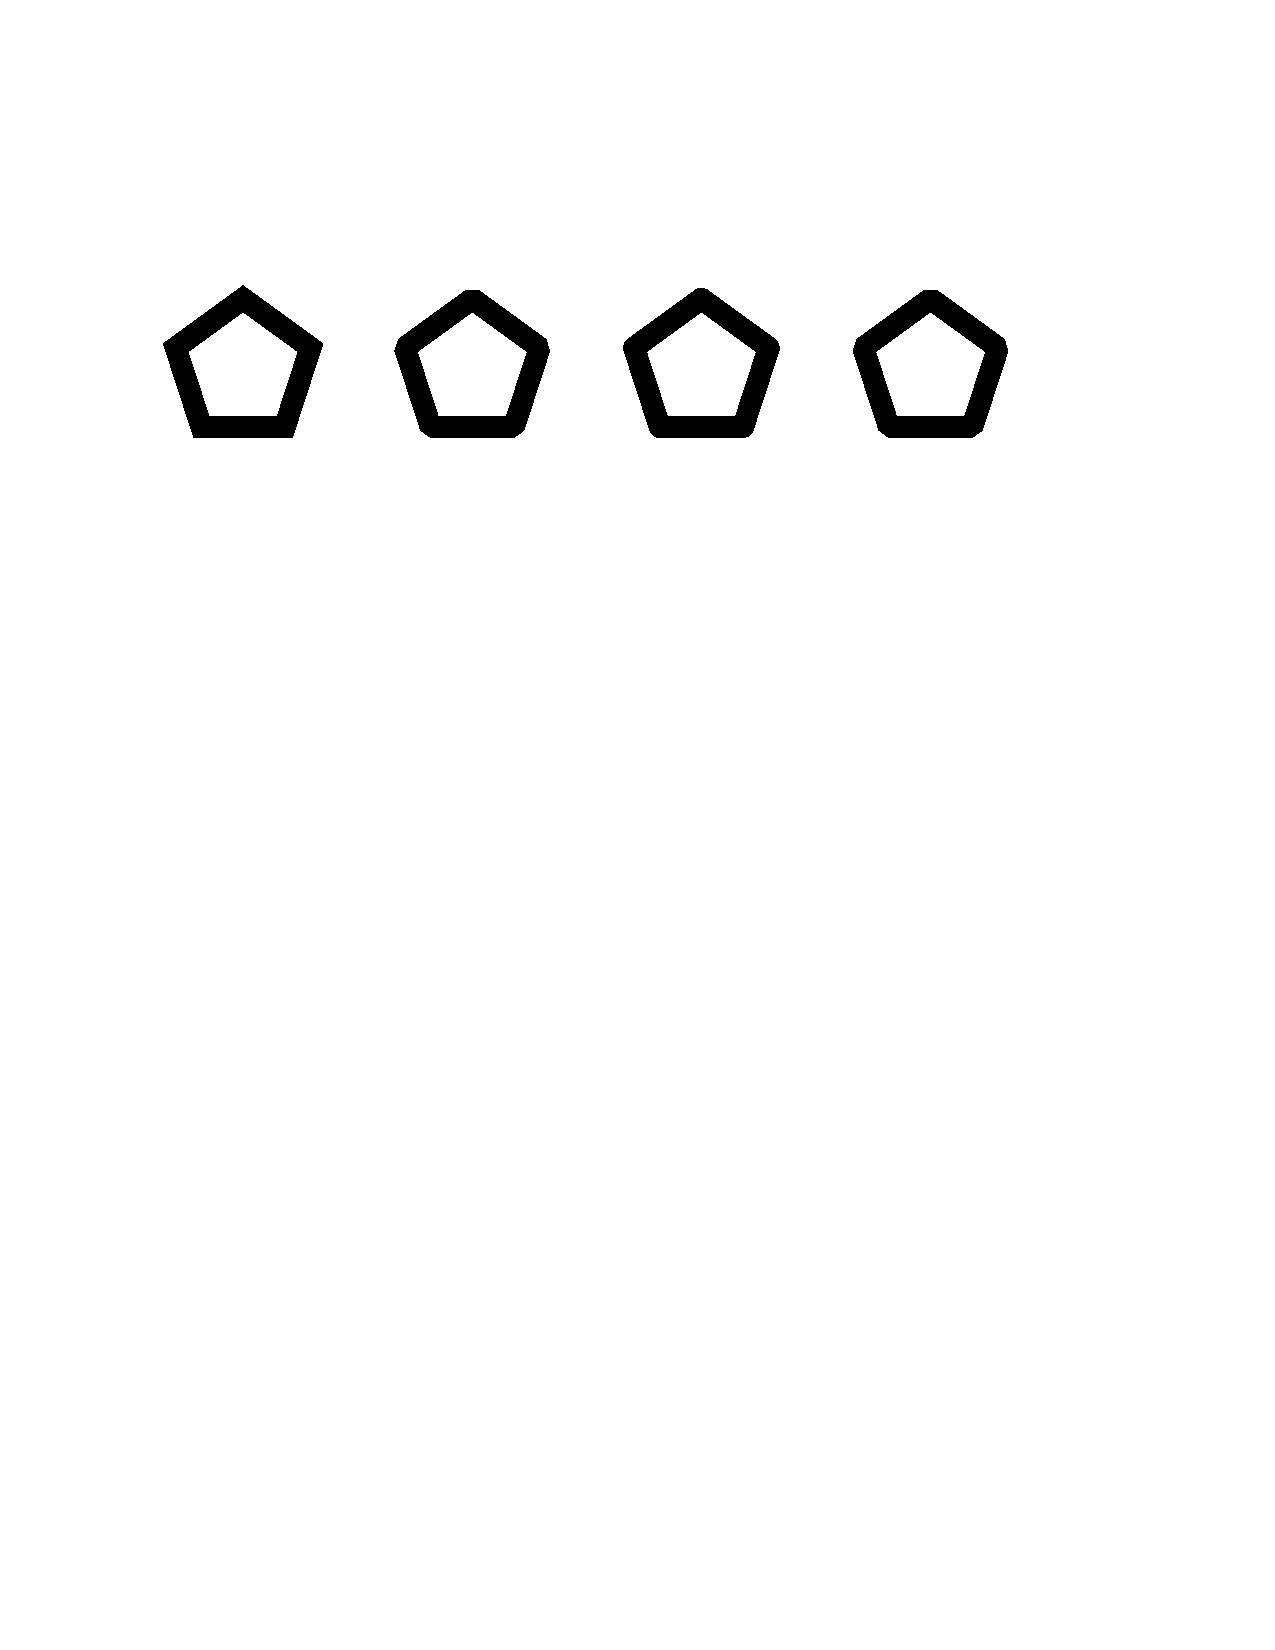
\includegraphics{line-joint-shapes}}
\caption{Line joint shapes.}
\end{figure}

\defoption {:line-cap-shape}
\Defgeneric {line-style-cap-shape} {line-style}

Specifies the shape for the ends of lines and arcs drawn by a drawing function,
one of \cl{:butt}, :\cl{square}, \cl{:round}, or \cl{:no-end-point}; the default
is \cl{:butt}.  Note that the cap shape is implemented by the host window
system, so not all platforms will necessarily fully support it.

\begin{figure}
\centerline{
\includegraphics{line-cap-shapes}}
\caption{Line cap shapes.}
\end{figure}

\defoption {:line-dashes}
\Defgeneric {line-style-dashes} {line-style}

Controls whether lines or arcs are drawn as dashed figures, and if so, what the
dashing pattern is.  Possible values are:

\begin{itemize}
\item \cl{nil}---lines are drawn solid, with no dashing.  This is the default.

\item \cl{t}---lines are drawn dashed, with a dash pattern that is unspecified
and may vary with the rendering engine.  This allows the underlying display
substrate to provide a default dashed line for the programmer whose only
requirement is to draw a line that is visually distinguishable from the default
solid line.

\item A sequence---specifies a sequence, usually a vector, controlling the dash
pattern of a drawing function.  It is an error if the sequence does not contain
an even number of elements.  The elements of the sequence are lengths (as real
numbers) of individual components of the dashed line or arc.  The odd elements
specify the length of inked components, the even elements specify the gaps.  All
lengths are expressed in the units described by \cl{line-style-unit}.
\end{itemize}

(See also \cl{make-contrasting-dash-patterns}.)

\subsection {Contrasting Dash Patterns}

\Defun {make-contrasting-dash-patterns} {n \optional k}

If \arg{k} is not supplied, this returns a vector of \arg{n} dash patterns with
recognizably different appearance.  Elements of the vector are guaranteed to be
acceptable values for \cl{:dashes}, and do not include \cl{nil}, but their class
is not otherwise specified.  The vector is a fresh object that may be modified.

If \arg{k} is supplied, it must be an integer between 0 and $\arg{n}-1$
(inclusive), in which case \cl{make-contrasting-dash-patterns} returns the
\arg{k}'th dash-pattern rather than returning a vector of dash-patterns.

If the implementation does not have \arg{n} different contrasting dash patterns,
\cl{make-contrasting-dash-patterns} signals an error.  This will not happen
unless \arg{n} is greater than eight.

\Defgeneric {contrasting-dash-pattern-limit} {port}

Returns the number of contrasting dash patterns that can be rendered on any
medium on the \term{port} \arg{port}.  Implementations are encouraged to make
this as large as possible, but it must be at least 8.  All classes that obey the
port protocol must implement a method for this generic function.

% -*- Mode: LaTeX; Package: CLIM-USER -*-

\chapter {Text Styles}
\label {text-styles}

When specifying a particular ``appearance'' for rendered characters, there is a
tension between portability and access to specific font for a display device.
CLIM provides a portable mechanism for describing the desired \concept{text
style} in abstract terms.  Each CLIM ``port'' defines a mapping between these
abstract style specifications and particular device-specific fonts.  In this
way, an application programmer can specify the desired text style in abstract
terms secure in the knowledge that an appropriate device font will be selected
at run time by CLIM.  However, some programmers may require direct access to
particular device fonts.  The text style mechanism supports specifying device
fonts by name, allowing the programmer to sacrifice portability for control.


\section {Text Styles}

Text style objects have components for family, face, and size.  Not all of these
attributes need be supplied for a given text style object.  Text styles can be
merged in much the same way as pathnames are merged; unspecified components in
the style object (that is, components that have \cl{nil} in them) may be filled
in by the components of a ``default'' style object.  A text style object is
called \concept{fully specified} if none of its components is \cl{nil}, and the
size component is not a relative size (that is, is neither \cl{:smaller} nor
\cl{:larger}).

\Defprotoclass {text-style}

The protocol class for text styles.
\IfYouWantClass {a} {text style} {text-style}

\Defpredicate {text-style-p} {object}

Returns \term{true} if \arg{object} is a \term{text style}, otherwise returns
\term{false}.

\Defclass {standard-text-style}

An instantiable class that implements text styles.  It is a subclass of
\cl{text-style}.  This is the class that \cl{make-text-style} instantiates.
\Immutable

The interface to text styles is as follows:

\Defun {make-text-style} {family face size}

Returns an object of class \cl{standard-text-style} with a family of
\arg{family}, a face of \arg{face}, and a size of \arg{size}.

\arg{family} is one of \cl{:fix}, \cl{:serif}, \cl{:sans-serif}, or \cl{nil}.

\arg{face} is one of \cl{:roman}, \cl{:bold}, \cl{:italic}, \cl{(:bold :italic)},
or \cl{nil}.

\arg{size} is a real number representing the size in printer's points, one of
the logical sizes (\cl{:normal}, \cl{:tiny}, \cl{:very-small}, \cl{:small},
\cl{:large}, \cl{:very-large}, \cl{:huge}), a relative size (\cl{:smaller} or
\cl{:larger}), or \cl{nil}.

Implementations are permitted to extend legal values for \arg{family},
\arg{face}, and \arg{size}.

\issue {York, SWM} {Need to describe what family, face, size mean in terms of
visual appearance.  This should also be reconciled with the ISO description of
the attributes of a ``text style'', including such things as underlining,
subscripts, superscripts, etc.}

\Defconst {*default-text-style*}

The default text style used on a CLIM medium if no text style it explicitly
specified for the medium when it it created.  This must be a fully merged text
style.

\Defconst {*undefined-text-style*}

The text style that is used as a fallback if no mapping exists for some other
text style when some text is about to be rendered on a display device (via
\cl{write-string} and \cl{draw-string*}, for example).  This text style should be fully
merged, and it must have a mapping for all display devices.


\subsection {Text Style Protocol and Text Style Suboptions}

The following generic functions comprise the text style protocol.  All
subclasses of \cl{text-style} must implement methods for each of these generic
functions.

Each of the suboptions described below has a corresponding reader accessor that
can be used to extract a particular component from a text style.

\Defgeneric {text-style-components} {text-style}

Returns the components of the \term{text style} \arg{text-style} as three
values, the family, face, and size.

\defoption {:text-family}
\Defgeneric {text-style-family} {text-style}

Specifies the family of the \term{text style} \arg{text-style}.

\defoption {:text-face}
\Defgeneric {text-style-face} {text-style}

Specifies the face of the \term{text style} \arg{text-style}.

\defoption {:text-size}
\Defgeneric {text-style-size} {text-style}

Specifies the size of the \term{text style} \arg{text-style}.


\Defun {parse-text-style} {style-spec}  

Returns a text style object.  \arg{style-spec} may be a \cl{text-style} object
or a device font, in which case it is returned as is, or it may be a list of the
family, face, and size (that is, a ``style spec''), in which case it is
``parsed'' and a \cl{text-style} object is returned.  This function is for
efficiency, since a number of common functions that take a style object as an
argument can also take a style spec, in particular \cl{draw-text}.


\Defgeneric {merge-text-styles} {style1 style2}

Merges the \term{text styles} \arg{style1} with \arg{style2}, that is, returns a
new text style that is the same as \arg{style1}, except that unspecified
components in \arg{style1} are filled in from \arg{style2}.  For convenience,
the two arguments may be also be style specs.

When merging the sizes of two text styles, if the size from \arg{style1} is a
relative size, the resulting size is either the next smaller or next larger size
than is specified by \arg{style2}.  The ordering of sizes, from smallest to
largest, is \cl{:tiny}, \cl{:very-small}, \cl{:small}, \cl{:normal},
\cl{:large}, \cl{:very-large}, and \cl{:huge}.

\issue {SWM} {Need to describe face-merging properly.  For example, merging a
bold face with an italic one can result in a bold-italic face.}


\defgeneric {text-style-ascent}  {text-style medium} 
\defgeneric {text-style-descent} {text-style medium}
\defgeneric {text-style-height}  {text-style medium}
\Defgeneric {text-style-width}   {text-style medium}

Returns the ascent, descent, height, and width (respectively) of the font
corresponding to the \term{text style} \arg{text-style} as it would be rendered
on the \term{medium} \arg{medium}.  \arg{text-style} must be a fully specified
text style.

The ascent of a font is the distance between the top of the tallest character in
that font and the font's baseline.  The descent of a font is the distance
between the baseline and the bottom of the lowest descending character (usually
``g'', ``p'', ``q'', or ``y'').  The height of a font is the sum of the ascent
and the descent of the font.  The width of a font is the width of some
representative character in the font.

The methods for these generic functions will typically specialize both the
\arg{text-style} and \arg{medium} arguments.  Implementations should also
provide ``trampoline'' for these generic functions on output sheets; the
trampolines will simply call the method for the medium.


\Defgeneric {text-style-fixed-width-p} {text-style medium}

Returns \term{true} if the \term{text styles} \arg{text-style} will map to a
fixed-width font on the \term{medium} \arg{medium}, otherwise returns
\term{false}.  \arg{text-style} must be a fully specified text style.

The methods for this generic function will typically specialize both the
\arg{text-style} and \arg{medium} arguments.  Implementations should also
provide a ``trampoline'' for this generic function for output sheets; the
trampoline will simply call the method for the medium.


\issue {SWM} {Discuss baselines?  Kerning?}


\Defgeneric {text-size} {medium string \key text-style (start \cl{0}) end} 

Computes the ``cursor motion'' in device units that would take place if
\arg{string} (which may be either a string or a character) were output to the
\term{medium} \arg{medium} starting at the position $(0,0)$.  Five values are
returned:  the total width of the string in device units, the total height of
the string in device units, the final $x$ cursor position (which is the same as
the width if there are no \verb+#\Newline+ characters in the string), the final
$y$ cursor position (which is 0 if the string has no \verb+#\Newline+ characters
in it, and is incremented by the line height of \arg{medium} for each
\verb+#\Newline+ character in the string), and the string's baseline.

\arg{text-style} specifies what text style is to be used when doing the output,
and defaults to \cl{medium-merged-text-style} of the medium.  \arg{text-style}
must be a fully specified text style.  \arg{start} and \arg{end} may be used to
specify a substring of \arg{string}.

If a programmer needs to account for kerning or the ascent or descent of the
text style, he should measure the size of the bounding rectangle of the text
rendered on \arg{medium}.

All mediums and output sheets must implement a method for this generic function.


\section {Text Style Binding Forms}

\Defmacro {with-text-style} {(medium text-style) \body body}

Binds the current text style of the \term{medium} designated by \arg{medium} to
correspond to the new text style.  \arg{text-style} may either a text style
object or a style spec (that is, a list of the a family, a face code, and a
size).  \arg{body} is executed with the new text style in effect.

The \arg{medium} argument is not evaluated, and must be a symbol that is bound
to a sheet or medium.  If \arg{medium} is \cl{t}, \cl{*standard-output*} is
used.  \arg{body} may have zero or more declarations as its first forms.

\cl{with-text-style} must be implemented by expanding into a call to
\cl{invoke-with-text-style}, supplying a function that executes \arg{body} as
the \arg{continuation} argument to \cl{invoke-with-text-style}.

\Defgeneric {invoke-with-text-style} {medium continuation text-style}

Binds the current text style of the \term{medium} \arg{medium} to correspond to
the new text style, and calls the function \arg{continuation} with the new text
style in effect.  \arg{text-style} may either a text style object or a style
spec (that is, a list of the a family, a face code, and a size).  \arg{continuation}
is a function of one argument, the medium; it has dynamic extent.

\arg{medium} can be a medium, a sheet that supports the sheet output protocol,
or a stream that outputs to such a sheet.  All classes that obey the medium
protocol must implement a method for \cl{invoke-with-text-style}.


\defmacro {with-text-family} {(medium family) \body body}
\defmacro {with-text-face}   {(medium face) \body body}
\Defmacro {with-text-size}   {(medium size) \body body}

Binds the current text style of the \term{medium} designated by \arg{medium} to
correspond to a new text style consisting of the current text style with the new
family, face, or size (respectively) merged in.  \arg{face}, \arg{family}, and
\arg{size} are as for \cl{make-text-style}.  \arg{body} is executed with the new
text style in effect.

The \arg{medium} argument is not evaluated, and must be a symbol that is bound
to a sheet or medium.  If \arg{medium} is \cl{t}, \cl{*standard-output*} is
used.  \arg{body} may have zero or more declarations as its first forms.

These macros are ``convenience'' forms of \cl{with-text-style} that must expand
into calls to \cl{invoke-with-text-style}.


\section {Controlling Text Style Mappings}

Text styles are mapped to fonts using the \cl{text-style-mapping} function,
which takes a port, a character set, and a text style and returns a font
object.  All ports must implement methods for the following generic functions,
for all classes of text style.

The objects used to represent a font mapping are unspecified and are likely to
vary from port to port.  For instance, a mapping might be some sort of font
object on one type of port, or might simply be the name of a font on another.

\issue {SWM} {We still need to describe what a device font is.  Ditto, character
sets.}

Part of initializing a port is to define the mappings between text styles and
font names for the port's host window system.

\Defgeneric {text-style-mapping} {port text-style \optional character-set}

Returns the font mapping that will be used when rendering characters in the
character set \arg{character-set} in the \term{text style} \arg{text-style} on
any medium on the \term{port} \arg{port}.  If there is no mapping associated
with \arg{character-set} and \arg{text-style} on \arg{port}, then some other
object will be returned that corresponds to the ``unmapped'' text style.

\arg{character-set} defaults to the standard character set.

\Defgeneric {(setf text-style-mapping)} {mapping port text-style \optional character-set} 

Sets the text style mapping for \arg{port}, \arg{character-set}, and
\arg{text-style} to \arg{mapping}.  \arg{port}, \arg{character-set}, and
\arg{text-style} are as for \cl{text-style-mapping}.  \arg{mapping} is either a
font name or a list of the form \cl{(:style \arg{family} \arg{face}
\arg{size})}; in the latter case, the given style is translated at runtime into
the font represented by the specified style.

\arg{character-set} defaults to the standard character set.

\Defun {make-device-font-text-style} {display-device device-font-name}

Returns a text style object that will be mapped directly to the specified device
font when text is output to a to the display device with this style.  Device
font styles do not merge with any other kind of style.

% -*- Mode: LaTeX; Package: CLIM-USER -*-

\chapter {Graphics}
\label {graphics}

\section {Overview of Graphics}

The CLIM graphic drawing model is an idealized model of graphical pictures.  The
model provides the language that application programs use to describe the
intended visual appearance of textual and graphical output.  Usually not all of
the contents of the screen are described using the graphic drawing model.  For
example, menus and scroll bars might be described in higher-level terms.

An important aspect of the CLIM graphic drawing model is its extreme device
independence.  The model describes ideal graphical images and ignores
limitations of actual graphics devices.  One consequence of this is that the
actual visual appearance of the screen can only be an approximation of the
appearance specified by the model.  Another consequence of this is that the
model is highly portable.

CLIM separates output into two layers, a text/graphics layer in which one
specifies the desired visual appearance independent of device resolution and
characteristics, and a rendering layer in which some approximation of the
desired visual appearance is created on the device.  Of course application
programs can inquire about the device resolution and characteristics if they
wish and modify their desired visual appearance on that basis.  (There is also a
third layer above these two layers, the adaptive toolkit layer where one
specifies the desired functionality rather than the desired visual appearance.)

\Issue {SWM} {There are still no functions to ask about device resolution and
characteristics.  What characteristics do we need to be able to get to besides
the obvious ones of resolution and ``color depth''.  Also, do we really need to
refer to the adaptive toolkit layer here?}

CLIM's drawing functions provide convenient ways to draw several commonly-used
shapes.

The interaction between graphics and output recording will be described in
Chapter~\ref{output-recording}.


\section {Definitions}

\paragraph {Drawing plane.}

A drawing plane is an infinite two-dimensional plane on which graphical output
occurs.  The drawing plane contains an arrangement of colors and opacities that
is modified by each graphical output operation.  It is not possible to read back
the contents of a drawing plane, except by examining the output-history.
Normally each window has its own drawing plane.

\paragraph {Coordinates.}

Coordinates are a pair of real numbers in implementation-defined units that
identify a point in the drawing plane.

\paragraph {Sheets and Mediums.}

In this chapter, we use a medium as a destination for output.  The medium has a
drawing plane, two designs called the medium's foreground and background, a
transformation, a clipping region, a line style, and a text style.  There are
per-medium, dynamically scoped, default drawing options.  Different medium
classes are provided to allow programmers to draw on different sorts of devices,
such as displays, printers, and virtual devices such as bitmaps.

Many sheets can be used for doing output, so the drawing functions can also take
a sheet as the output argument.  In this case, the drawing function ``trampolines''
to the sheet's medium.  So, while the functions defined here are specified to be
called on mediums, they can also be called on sheets.

A stream is a special kind of sheet that implements the stream protocol; streams
include additional state such as the current text cursor (which is some point in
the drawing plane).

By default, the ``fundamental'' coordinate system of a CLIM stream (not a
general sheet or medium, whose fundamental coordinate system is not defined) is
a left handed system with $x$ increasing to the right, and $y$ increasing
downward.  $(0,0)$ is at the upper left corner.


\section {Drawing is Approximate}

Note that although the drawing plane contains an infinite number of mathematical
points, and drawing can be described as an infinite number of color and opacity
computations, the drawing plane cannot be viewed directly and has no material
existence.  It is only an abstraction.  What can be viewed directly is the
result of rendering portions of the drawing plane onto a medium.  No infinite
computations or objects of infinite size are required to implement CLIM, because
the results of rendering have finite size and finite resolution.

A drawing plane is described as having infinitely fine spatial, color, and
opacity resolution, and as allowing coordinates of unbounded positive or
negative magnitude.  A viewport into a drawing plane, on the other hand, views
only a finite region (usually rectangular) of the drawing plane.  Furthermore, a
viewport has limited spatial resolution and can only produce a limited number of
colors.  These limitations are imposed by the display hardware on which the
viewport is displayed.  A viewport also has limited opacity resolution,
determined by the finite arithmetic used in the drawing engine (which may be
hardware or software or both).

Coordinates are real numbers in implementation-defined units.  Often these units
equal the spatial resolution of a viewport, so that a line of thickness 1 is
equivalent to the thinnest visible line.  However, this equivalence is not
required and should not be assumed by application programs.

A valid CLIM implementation can be quite restrictive in the size and resolution
of its viewports.  For example, the spatial resolution might be only a few dozen
points per inch, the maximum size might be only a few hundred points on a side,
and there could be as few as two displayable colors (usually black and white).
The fully transparent and fully opaque opacity levels must always be supported,
but a valid CLIM implementation might support only a few opacity levels in
between (or possibly even none).  A valid CLIM implementation might implement
color blending and unsaturated colors by stippling, although it is preferred,
when possible, for a viewport to display a uniform color as a uniform color
rather than as a perceptible stipple.

When CLIM records the output to a sheet, there are no such limitations since
CLIM just remembers the drawing operations that were performed, not the results
of rendering.

CLIM provides some ways to ask what resolution limits are in effect for a
medium.  See Chapter~\ref{drawing-options} for their descriptions.

The application programmer uses the CLIM graphic drawing model as an interface
to describe the intended visual appearance.  An implementation does its best to
approximate that ideal appearance in a viewport, within its limitations of
spatial resolution, color resolution, number of simultaneously displayable
colors, and drawing speed.  This will usually require tradeoffs, for example
between speed and accuracy, and each implementation must make these tradeoffs
according to its own hardware/software environment and user concerns.  For
example, if the actual device supports a limited number of colors, the desired
color may be approximated by techniques such as dithering or stippling.  If the
actual device cannot draw curves exactly, they may be approximated, with or
without anti-aliasing.  If the actual device has limited opacity resolution,
color blending may be approximate.  A viewport might display colors that don't
appear in the drawing plane, both because of color and opacity approximation and
because of anti-aliasing at the edges of drawn shapes.

It is likely that different implementations will produce somewhat different
visual appearance when running the same application.  If an application requires
more detailed control, it must resort to a lower-level interface, and will
become less portable as a result.  These lower-level interfaces will be
documented on a per-platform basis.

Drawing computations are always carried out ``in color'', even if the viewport
is only capable of displaying black and white.  In other words, the CLIM drawing
model is always the fully general model, even if an implementation's color
resolution is limited enough that full use of the model is not possible.  Of
course an application that fundamentally depends on color will not work well on
a viewport that cannot display color.  Other applications will degrade
gracefully.

Whether the implementation uses raster graphics or some other display technique
is invisible at this interface.  CLIM does not specify the existence of pixels
nor the exact details of scan conversion, which will vary from one drawing
engine to the next.

Performance will also vary between implementations.  This interface is defined
in terms of simple conceptual operations, however an actual implementation may
use caching, specialized object representations, and other optimizations to
avoid materializing storage-intensive or computation-costly intermediate results
and to take advantage of available hardware.


\section {Rendering Conventions for Geometric Shapes}

The intent of this section is to describe the conventions for how CLIM should
render a shape on a display device.  These conventions and the accompanying
examples are meant to describe a set of goals that a CLIM implementation should
try to meet.  However, compliant CLIM implementations may deviate from these
goals if necessary (for example, if the rendering performance on a specific
platform would be unacceptably slow if these goals were met exactly and
implementors feel that users would be better served by speed than by accuracy).
Note that we discuss only pixel-based display devices here, which are the most
common, but by no means the only, sort of display device that can be supported
by CLIM.

When CLIM draws a geometric shape on some sort of display device, the idealized
geometric shape must somehow be rendered on the display device.  The geometric
shapes are made up of a set of mathematical points, which have no size; the
rendering of the shape is usually composed of pixels, which are roughly square.
These pixels exist in ``device coordinates'', which are gotten by transforming
the user-supplied coordinates by all of the user-supplied transformation, the
medium transformation, and the transformation that maps from the sheet to the
display device.  (Note that if the last transformation is a pure translation
that translates by an integer multiple of device units, then it has no effect on
the rendering other than placement of the figure drawn on the display device.)

Roughly speaking, a pixel is affected by drawing a shape only when it is inside
the shape (we will define what we mean by ``inside'' in a moment).  Since pixels
are little squares and the abstract points have no size, for most shapes there
will be many pixels that lie only partially inside the shape.  Therefore, it is
important to describe the conventions used by CLIM as to which pixels should be
affected when drawing a shape, so that the proper interface to the per-platform
rendering engine can be constructed.  (It is worth noting that on devices that
support color or grayscale, the rendering engine may attempt to draw a pixel
that is partially inside the shape darker or lighter, depending on how much of
it is inside the shape.  This is called \concept{anti-aliasing}.)  The conventions
used by CLIM is the same as the conventions used by X11:

\begin{itemize}
\item A pixel is a addressed by its upper-left corner.

\item A pixel is considered to be \concept{inside} a shape, and hence affected
by the rendering of that shape, if the center of the pixel is inside the shape.
If the center of the pixel lies exactly on the boundary of the shape, it is
considered to be inside if the inside of the shape is immediately to the right
(increasing $x$ direction on the display device) of the center point of the
pixel.  If the center of the pixel lies exactly on a horizontal boundary, it is
considered to be inside if the inside of the shape is immediately below
(increasing $y$ direction on the display device) the center point of the pixel.

\item An unfilled shape is drawn by taking the filled shape consisting of those
points that are within 1/2 the line thickness from the outline curve (using a
normal distance function, that is, the length of the line drawn at right angles
to the tangent to the outline curve at the nearest point), and applying the
second rule, above.
\end{itemize}

It is important to note that these rules imply that the decision point used for
insideness checking is offset from the point used for addressing the pixel by
half a device unit in both the $x$ and $y$ directions.  It is worth considering
the motivations for these conventions.

When two shapes share a common edge, it is important that only one of the shapes
own any pixel.  The two triangles in Figure~\ref{two-triangles} illustrate this.
The pixels along the diagonal belong to the lower figure.  When the decision
point of the pixel (its center) lies to one side of the line or the other, there
is no issue.  When the boundary passes through a decision point, which side the
inside of the figure is on is used to decide.  These are the triangles that CLIM
implementations should attempt to draw in this case.

\begin{figure}
\centerline{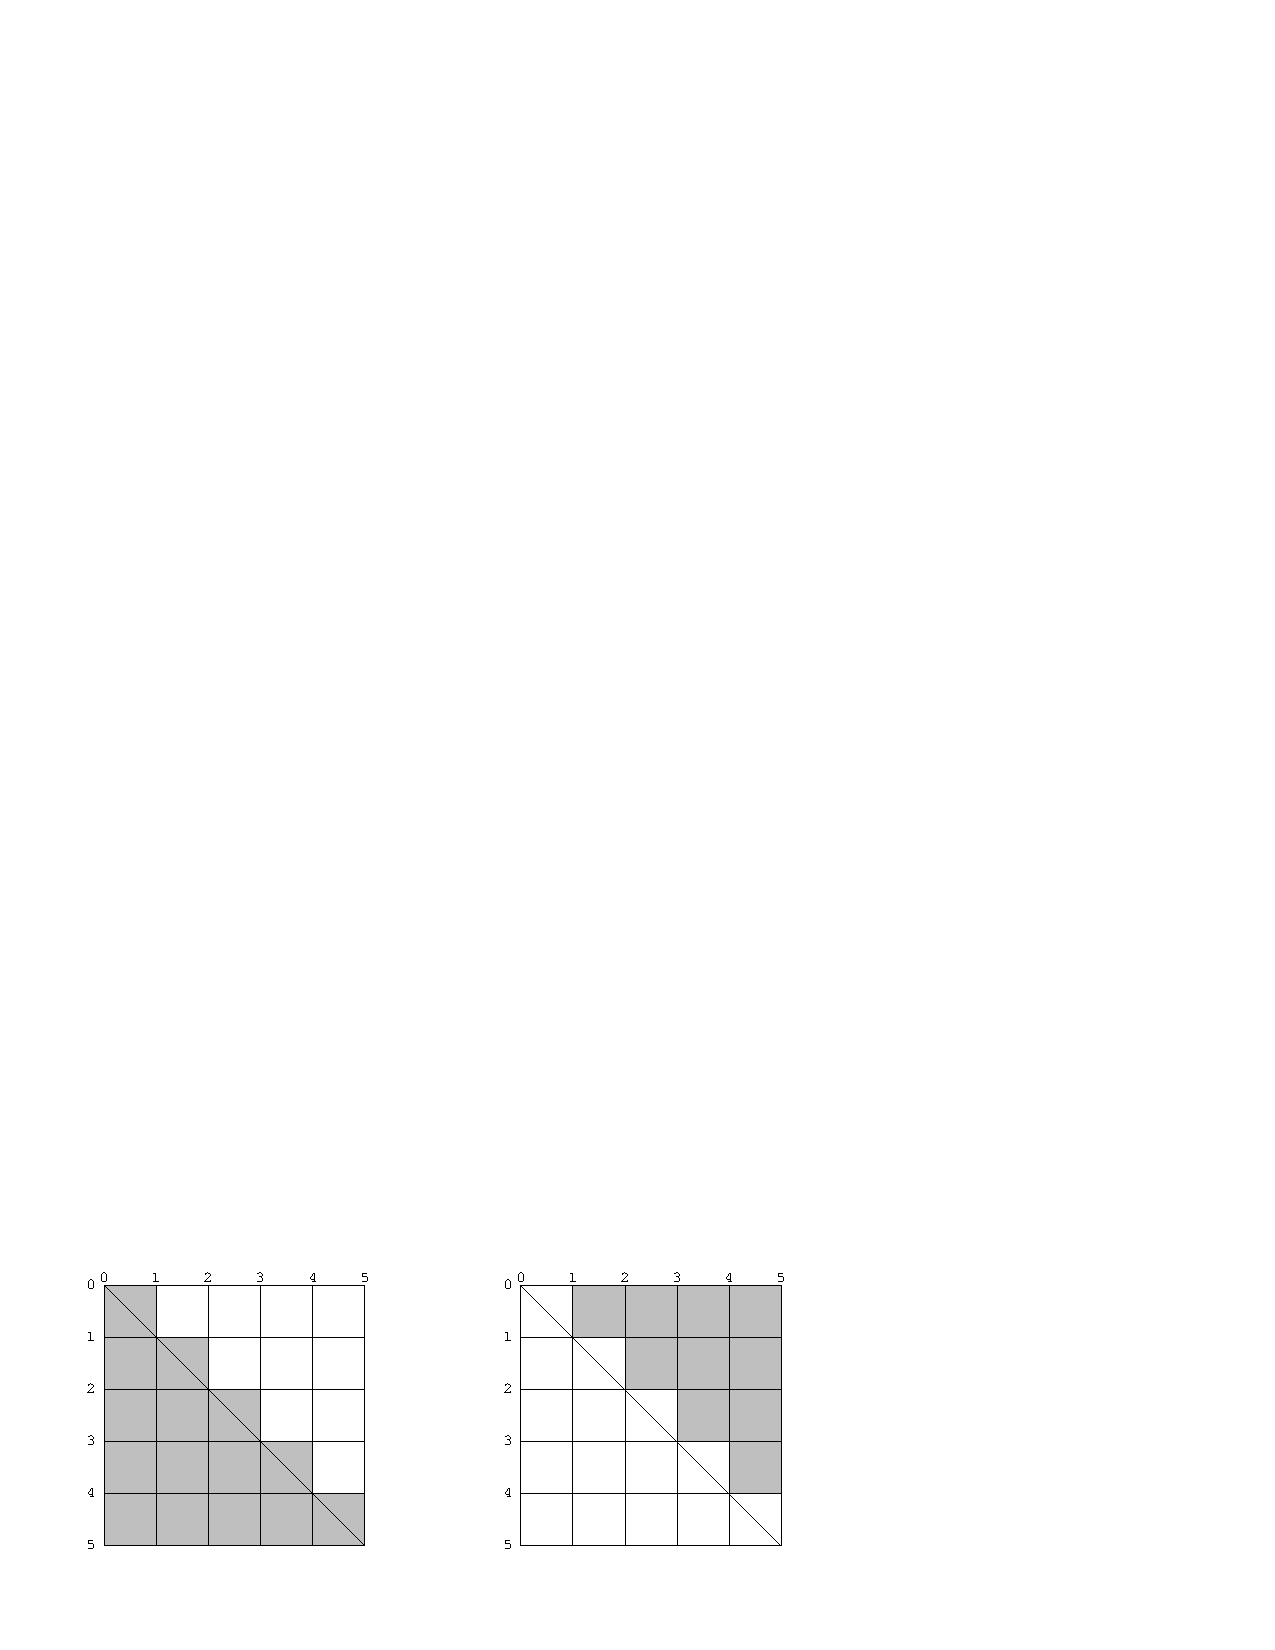
\includegraphics{two-triangles}}
\caption{\label{two-triangles} Pixel assignment with boundary on decision points.}
\end{figure}

The reason for choosing the decision point half a pixel offset from the address
point is to reduce the number of common figures (such as rectilinear lines and
rectangles with integral coordinates) that invoke the boundary condition rule.
This usually leads to more symmetrical results.  For instance, in
Figure~\ref{corner-circle}, we see a circle drawn when the decision point is the
same as the address point.  The four lighter points are indeterminate: it is not
clear whether they are inside or outside the shape.  Since we want to have each
boundary case determined according to which side has the figure on it, and since
we must apply the same rule uniformly for all figures, we have no choice but to
pick only two of the four points, leading to an undesirable lopsided figure.

\begin{figure}
\centerline{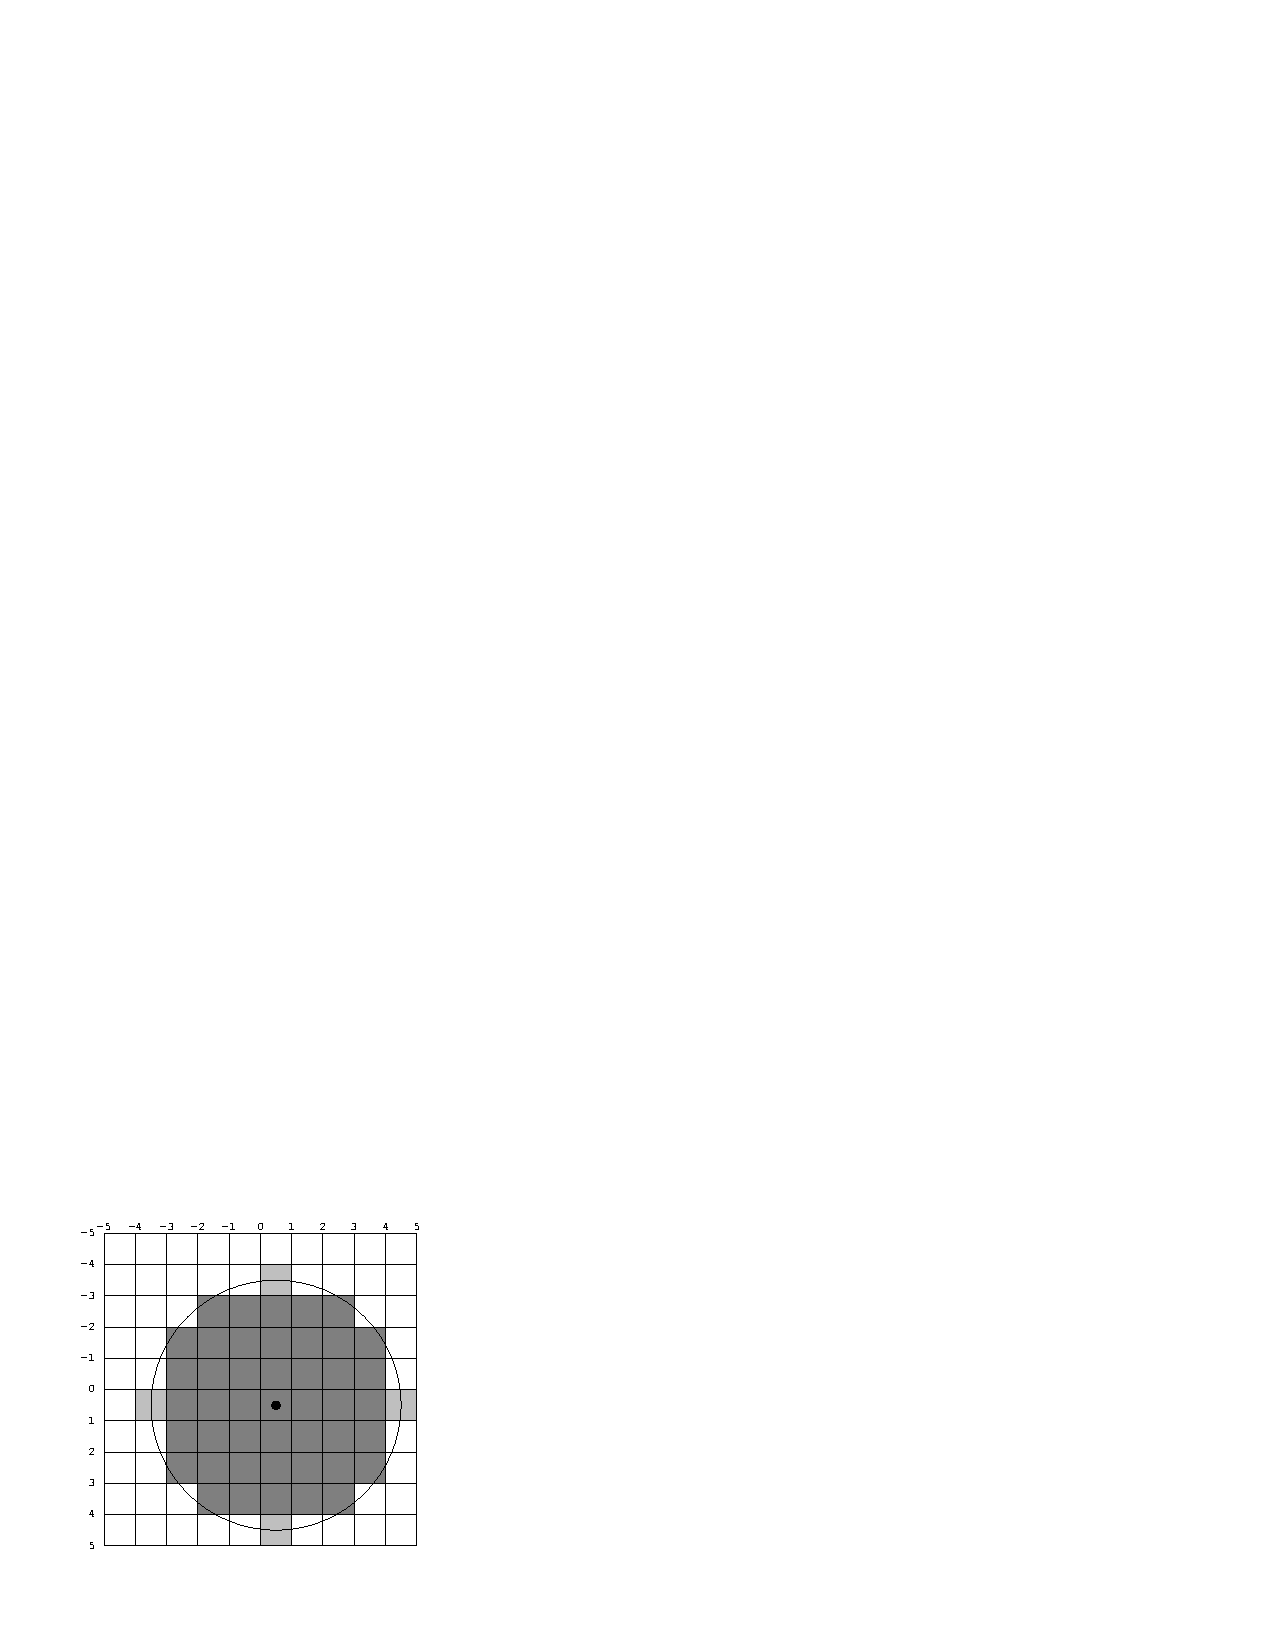
\includegraphics{corner-circle}}
\caption{\label{corner-circle} Choosing any two of the shaded pixels causes asymmetry.}
\end{figure}

If we had instead chosen to take all four boundary points, we would have a nice
symmetrical figure.  However, since this figure is symmetrical about a whole
pixel, it is one pixel wider than it ought to be.  The problem with this can be
seen clearly in Figure~\ref{inscribed-circle} if we attempt to draw a rectangle
and circle overlaid with the following code:

\begin{verbatim}
(defun draw-test (medium radius)
  (draw-circle* medium 0 0 radius :ink +foreground-ink+)
  (draw-rectangle* medium (- radius) (- radius) (+ radius) (+ radius)
                   :ink +flipping-ink+))
\end{verbatim}

\begin{figure}
\centerline{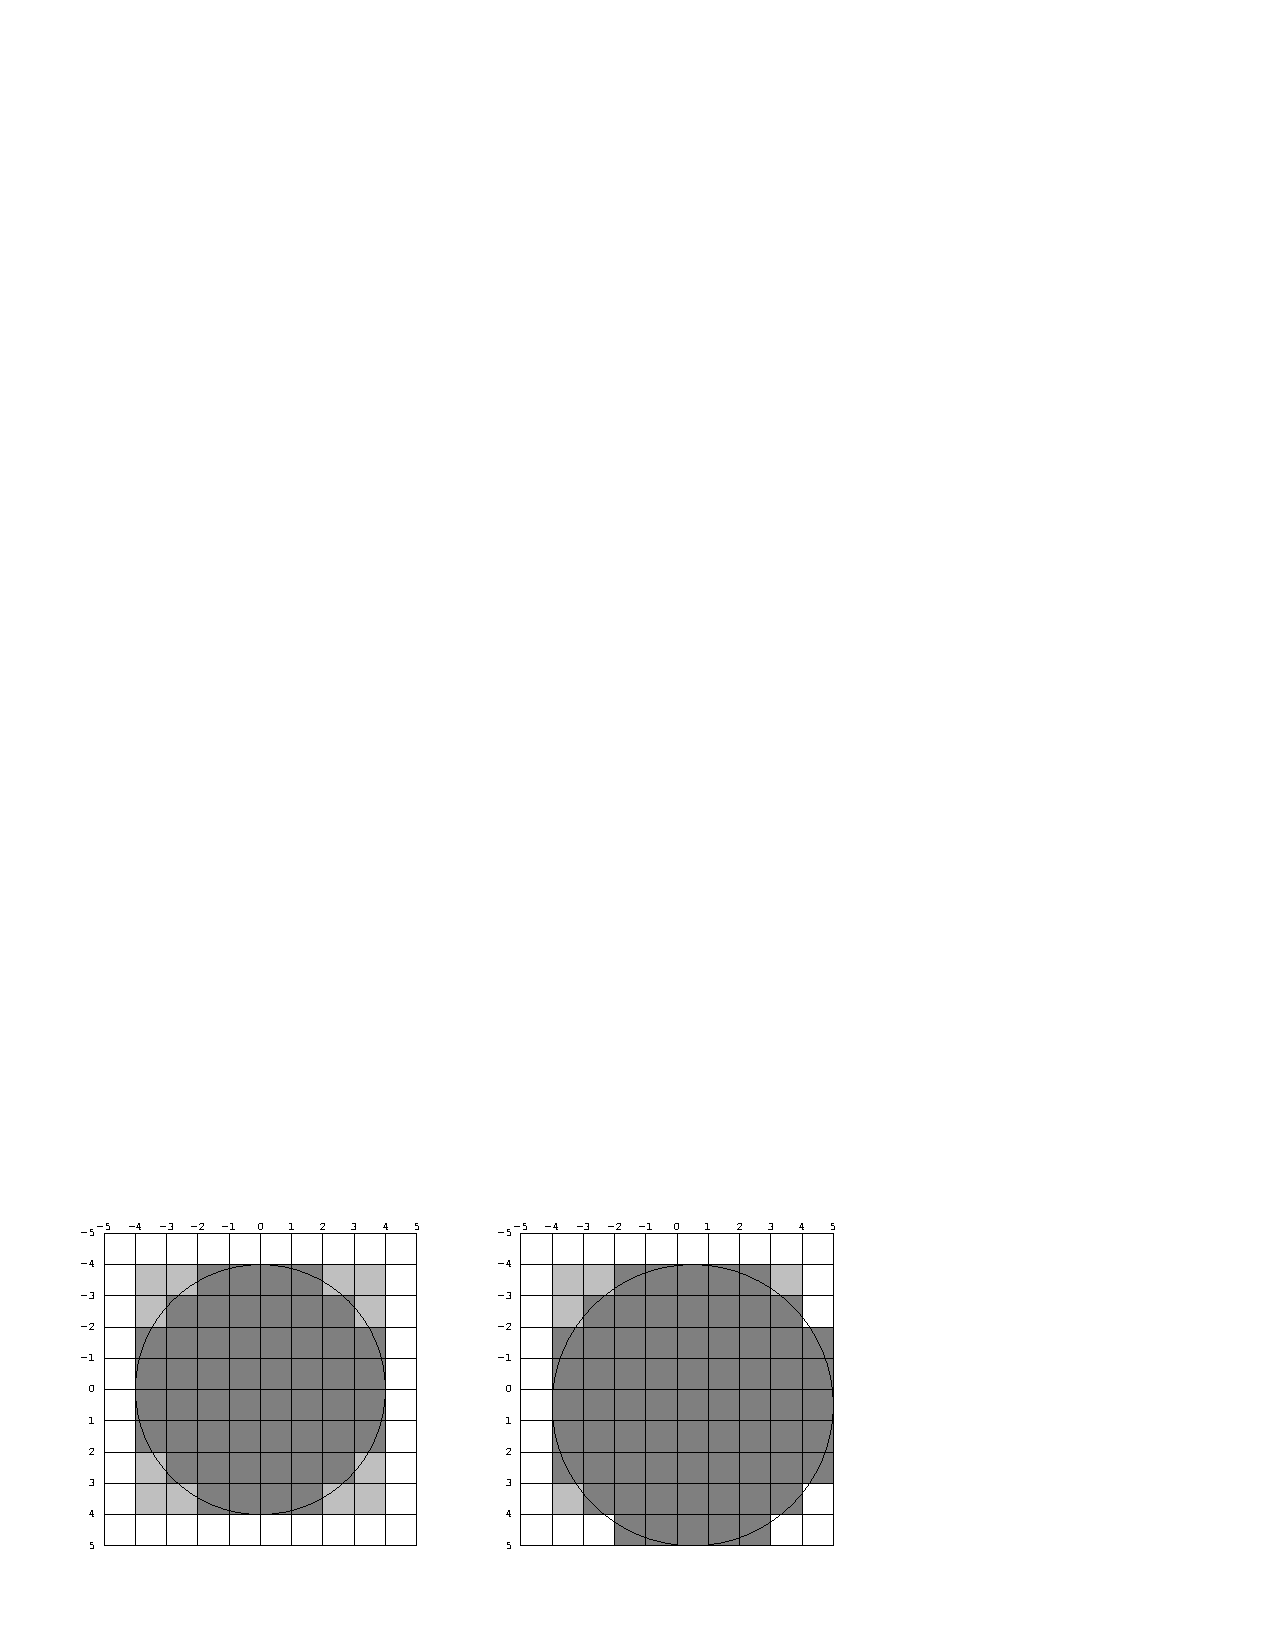
\includegraphics{inscribed-circle}}
\caption{\label{inscribed-circle} Two forms of a circle inscribed in a rectangle.}
\end{figure}

It is for this reason that we choose to have the decision point at the center of
the pixel.  This draws circles that look like the one in
Figure~\ref{correct-circle}.  It is this shape that CLIM implementations should
attempt to draw.

\begin{figure}
\centerline{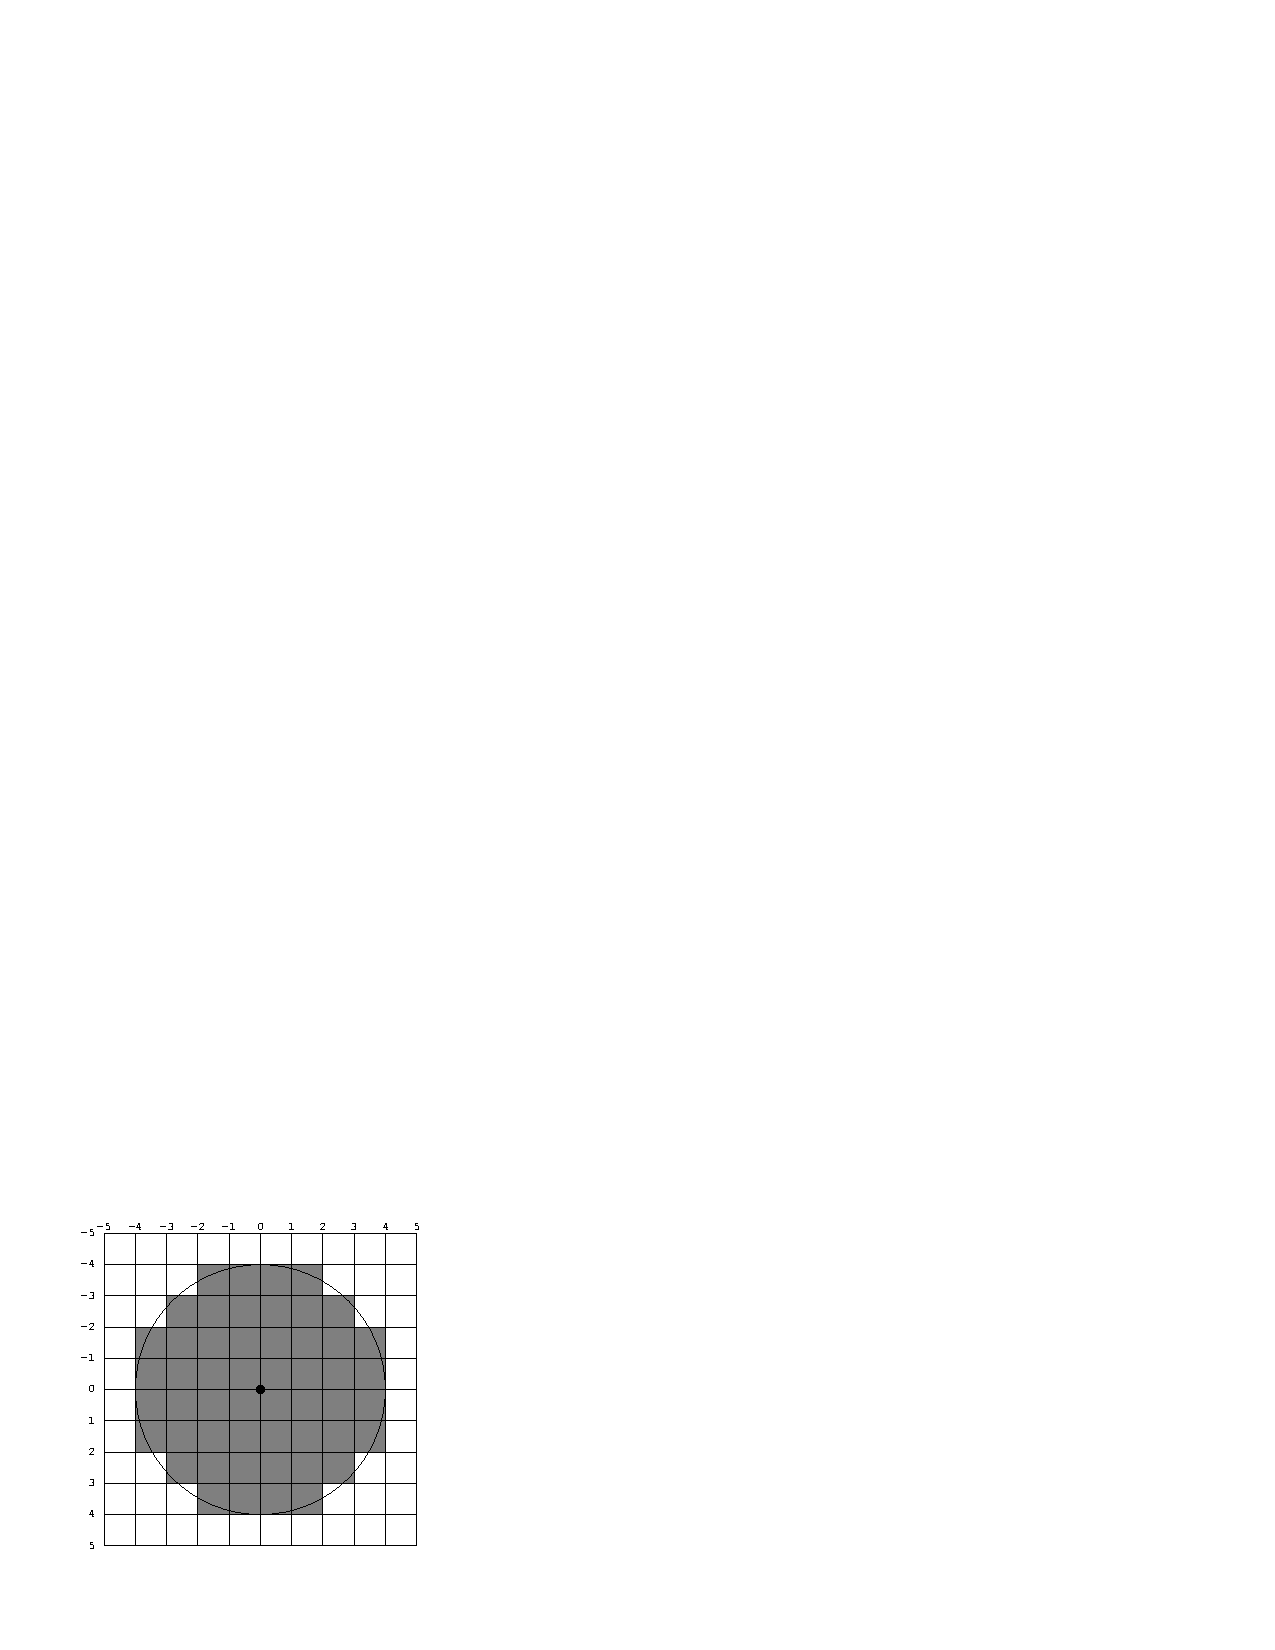
\includegraphics{correct-circle}}
\caption{\label{correct-circle} An aesthetically pleasing circle.}
\end{figure}

A consequence of these rendering conventions is that, when the start or end
coordinate (minus 1/2 the line thickness, if the shape is a path) is not an
integer, then rendering is not symmetric under reflection transformations.  Thus
to correctly and portably draw an outline of thickness 1 around a (rectilinear)
rectangular area with integral coordinates, the outline path must have
half-integral coordinates.  Drawing rectilinear areas whose boundaries are not
on pixel boundaries cannot be guaranteed to be portable.  Another way to say the
same thing is that the ``control points'' for a rectangular area are at the
corners, while the control points for a rectilinear path are in the center of
the path, not at the corners.  Therefore, in order for a path and an area to
abut seamlessly, the coordinates of the path must be offset from the coordinates
of the area by half the path's thickness.

\subsection {Permissible Alternatives During Rendering}

Some platforms may distinguish between lines of the minimum thinness from lines
that are thicker than that.  The two rasterizations depicted in
Figure~\ref{thin-lines} are both perfectly reasonable rasterizations of tilted
lines that are a single device unit wide.  The right-hand line is drawn as a
tilted rectangle, the left as the ``thinnest visible'' line.

\begin{figure}
\centerline{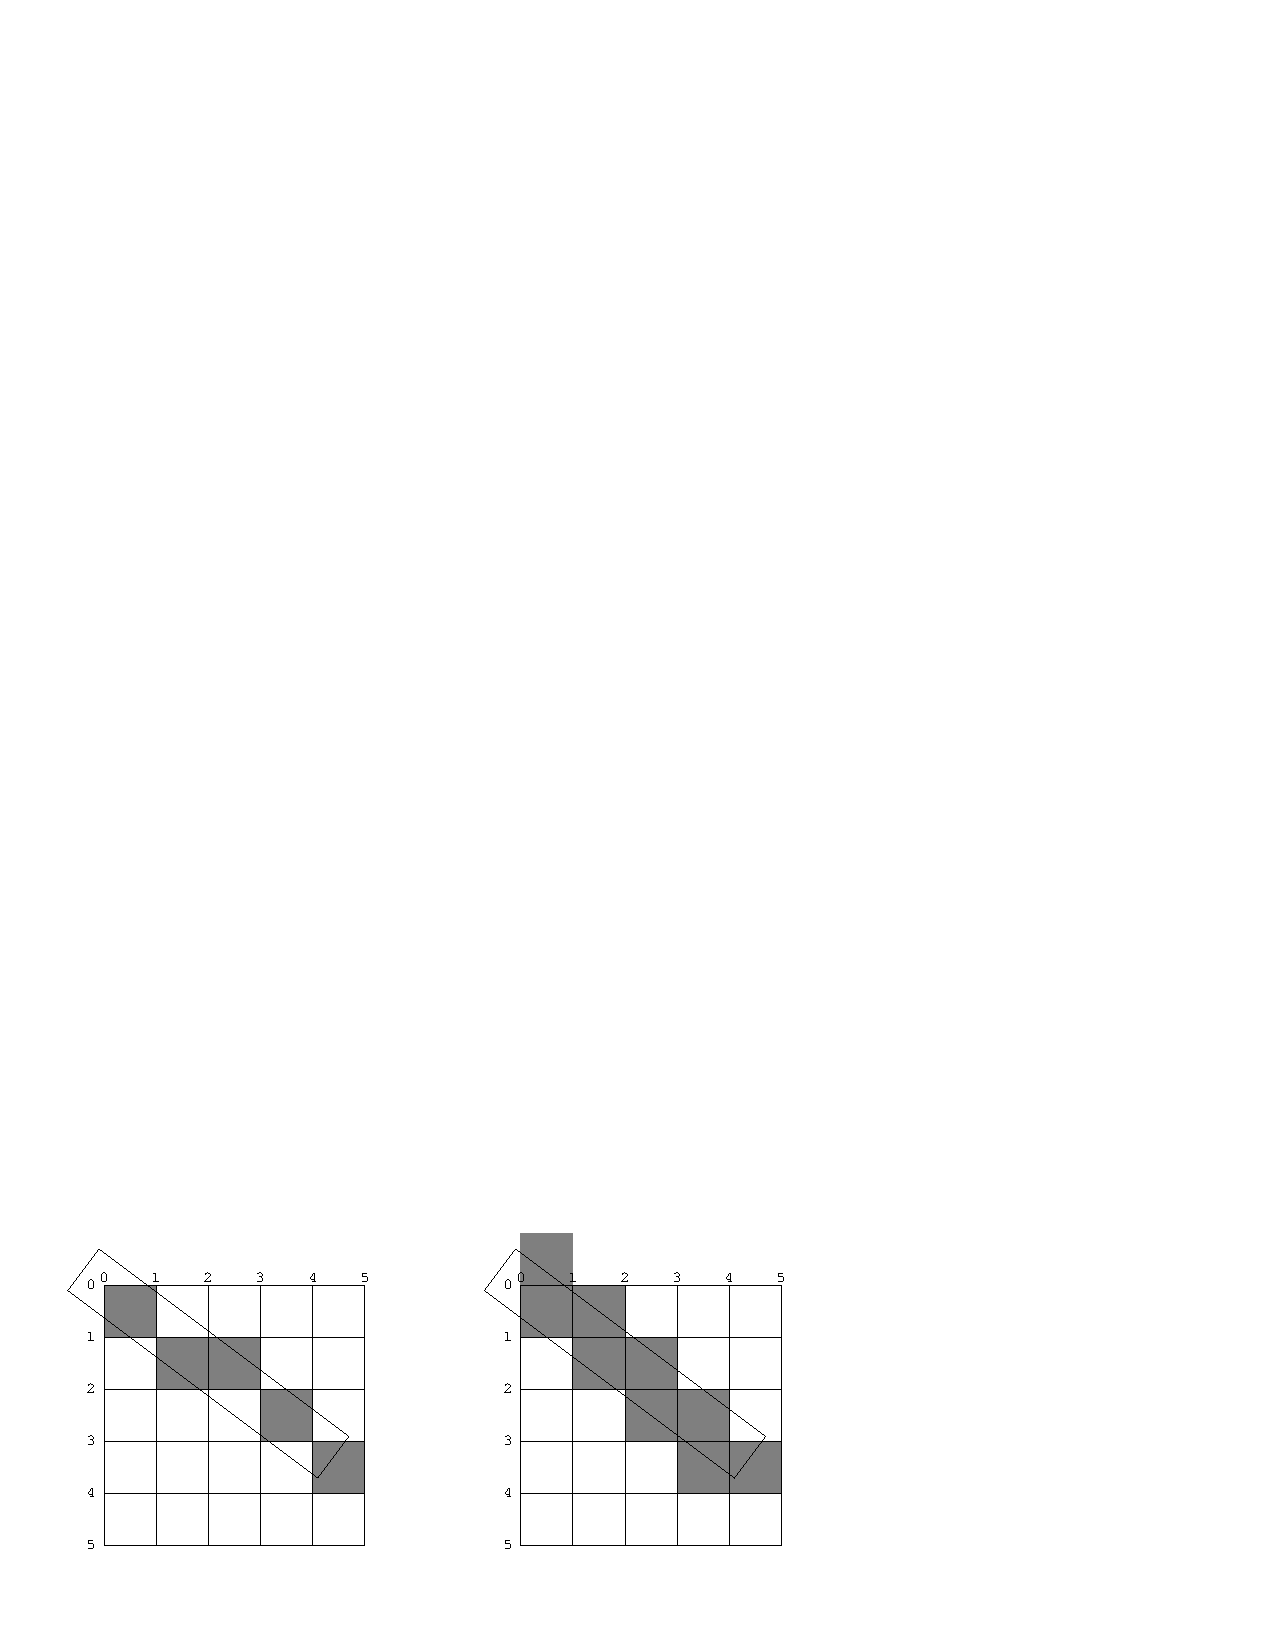
\includegraphics{thin-lines}}
\caption{\label{thin-lines} Two examples of lines of thickness 1.}
\end{figure}

For thick lines, a platform may choose to draw the exact tilted fractional
rectangle, or the coordinates of that rectangle might be rounded so that it is
distorted into another polygonal shape.  The latter case may be prove to be
faster on some platforms.  The two rasterizations depicted in
Figure~\ref{thick-lines} are both reasonable.

\begin{figure}
\centerline{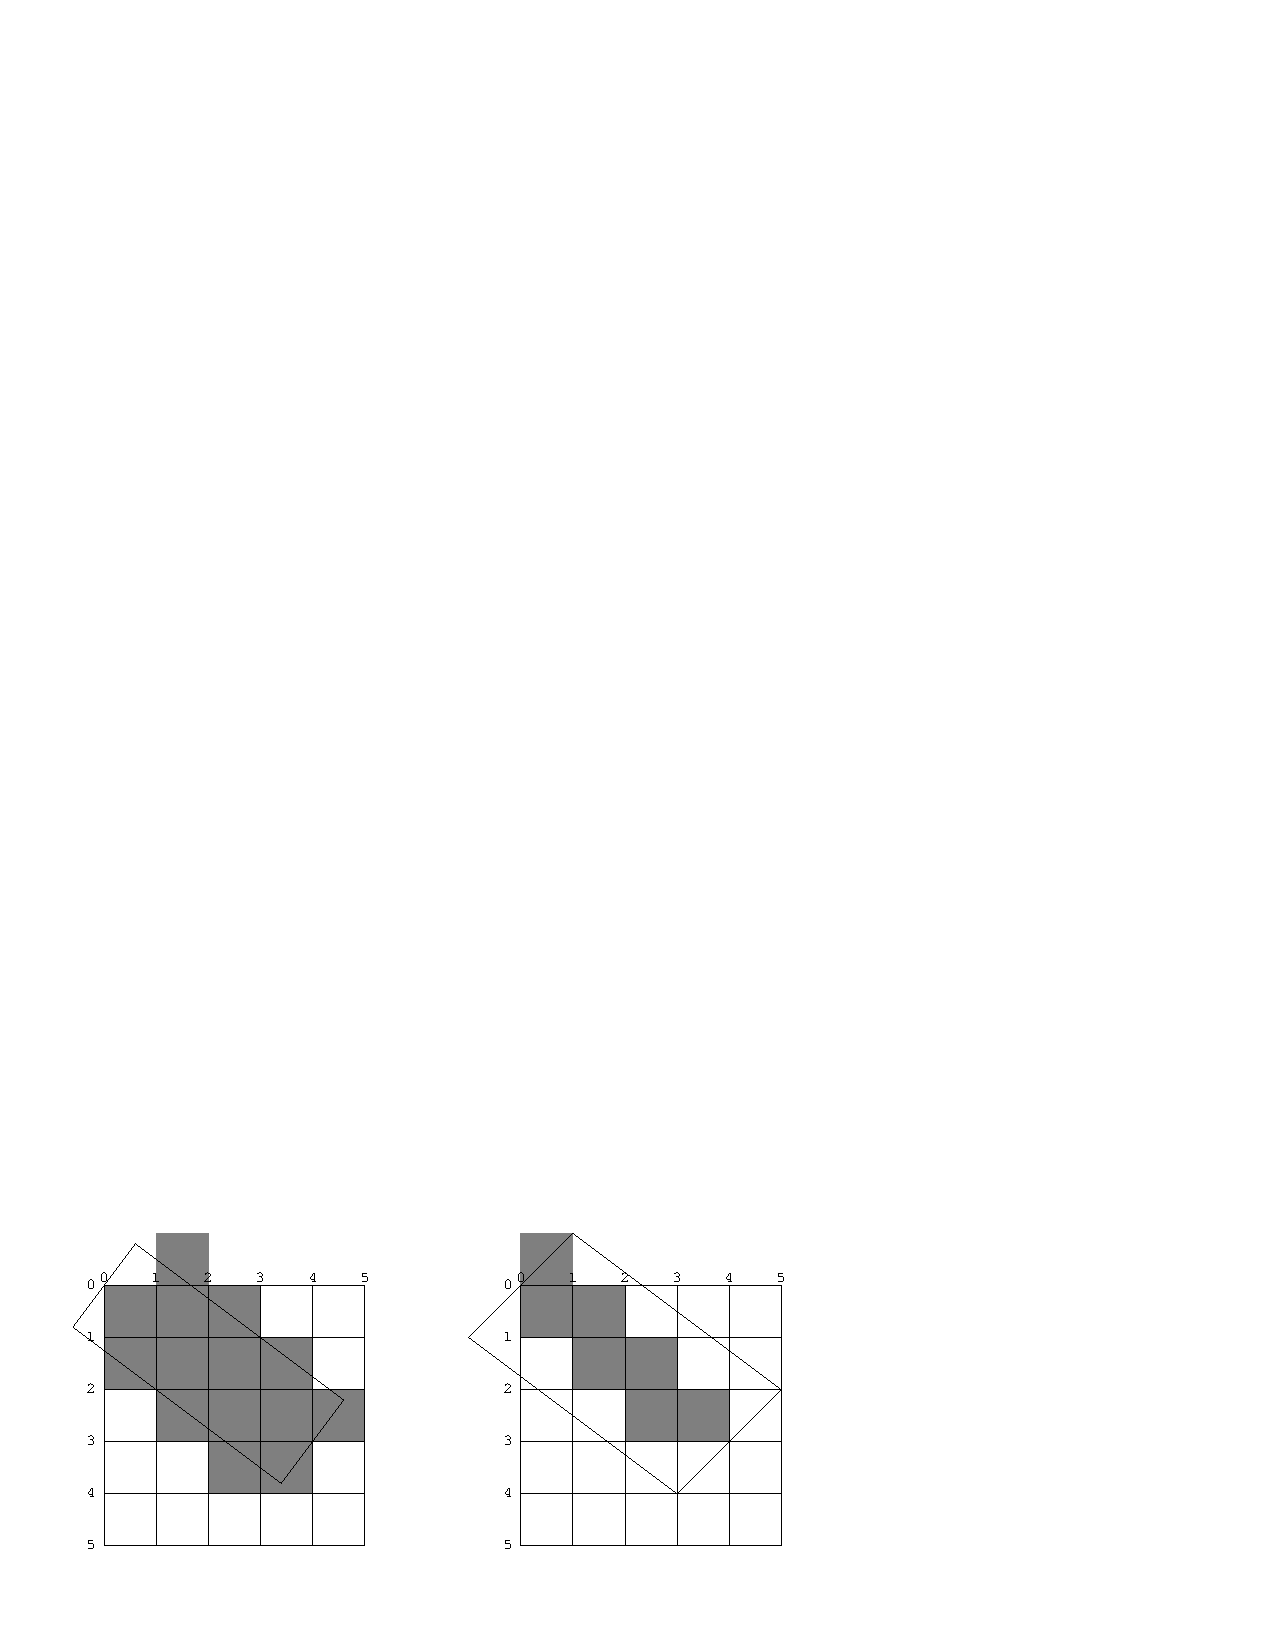
\includegraphics{thick-lines}}
\caption{\label{thick-lines} Two examples of lines of thickness 2.}
\end{figure}

The decision about which side of the shape to take when a boundary line passes
through the decision point is made arbitrarily, although we have chosen to be
compatible with the X11 definition.  This is not necessarily the most convenient
decision.  The main problem with this is illustrated by the case of a horizontal
line (see Figure~\ref{horizontal-lines}).  Our definition chooses to draw the
rectangular slice above the coordinates, since those pixels are the ones whose
centers have the figure immediately above them.  This definition makes it
simpler to draw rectilinear borders around rectilinear areas.

\begin{figure}
\centerline{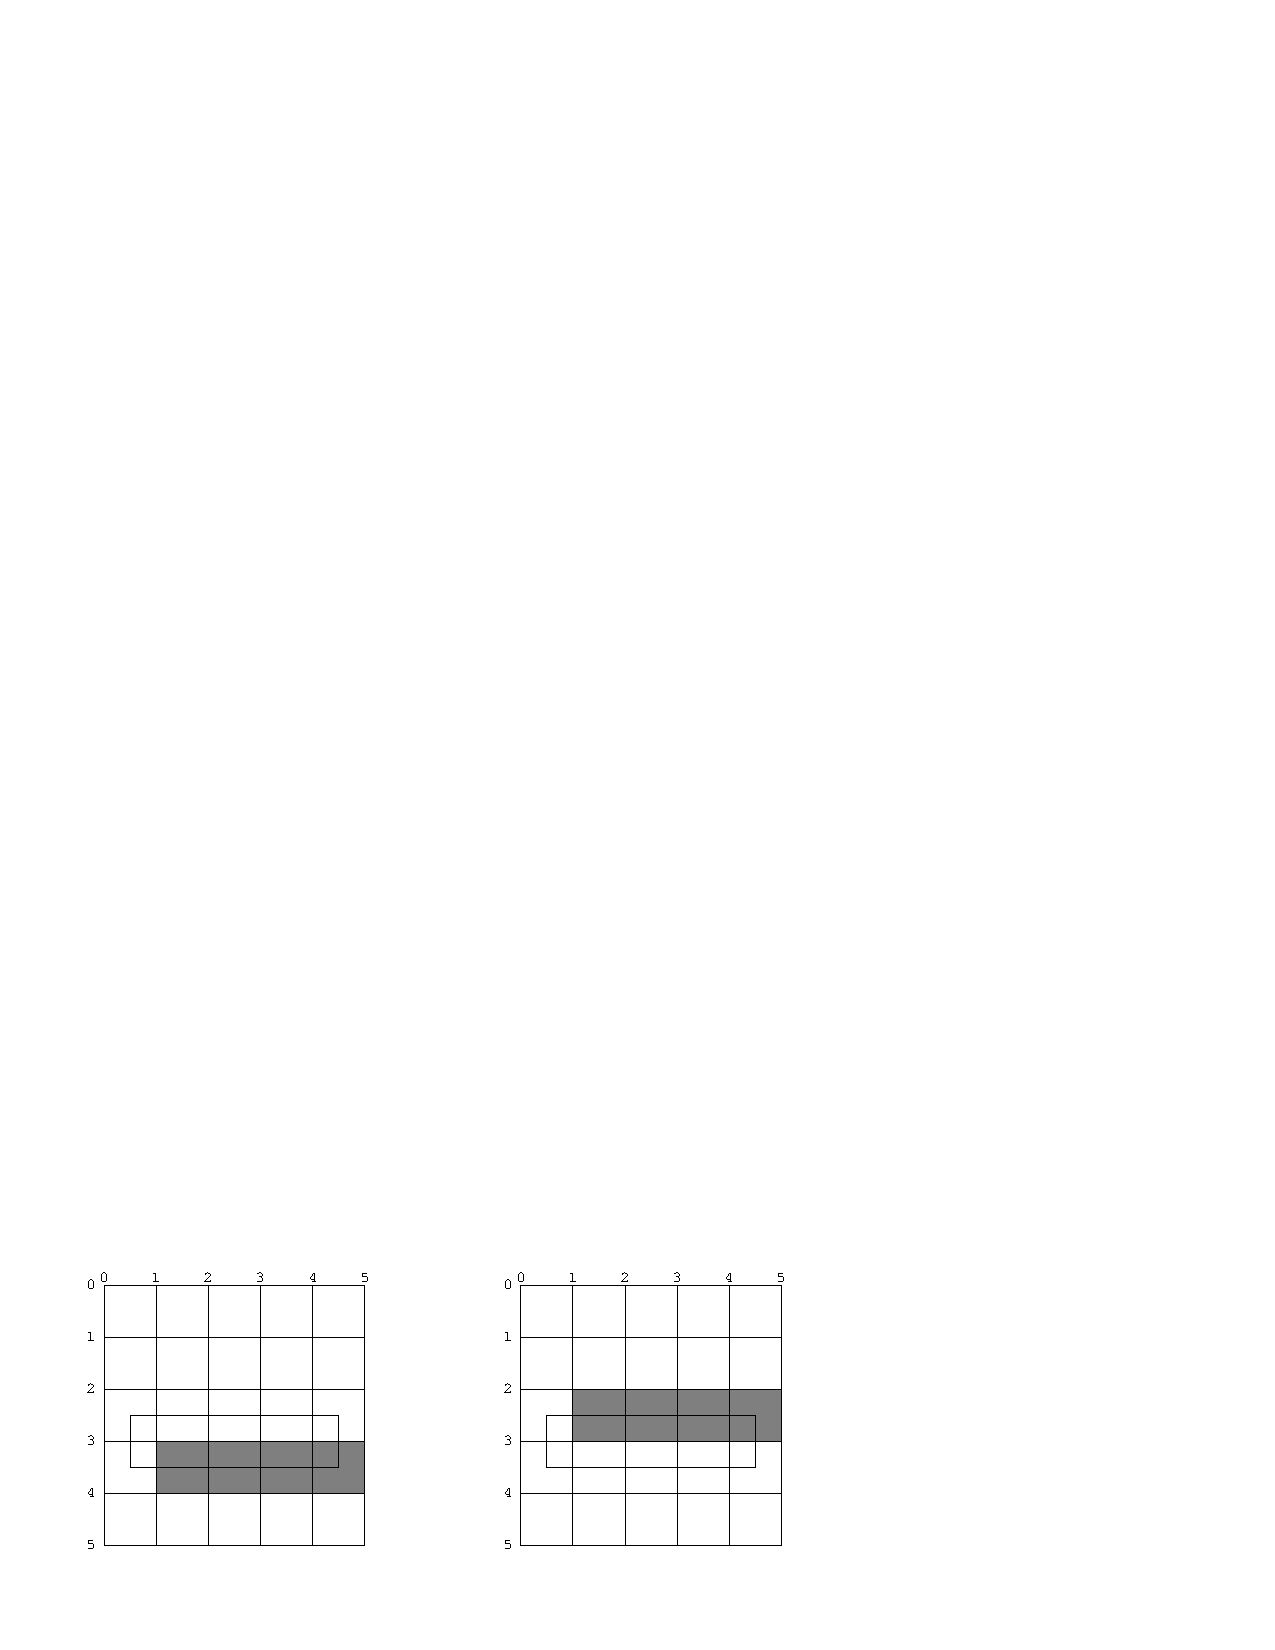
\includegraphics{horizontal-lines}}
\caption{\label{horizontal-lines} Two possible definitions of horizontal lines. 
Left figure is X11 definition.}
\end{figure}


\section {Drawing Functions\label{drawing-functions}}

\def\DrawingOptions{ink clipping-region transformation\ }
\def\PointOptions{line-style line-thickness line-unit}
\def\LineCapOptions{line-style line-thickness line-unit line-dashes line-cap-shape}
\def\LineJointOptions{line-style line-thickness line-unit line-dashes line-joint-shape}
\def\LineJointCapOptions{line-style line-thickness line-unit line-dashes line-joint-shape line-cap-shape}
\def\TextOptions{text-style text-family text-face text-size}

Each drawing function takes keyword arguments allowing any drawing option or
suboption to be supplied separately in the call to the function.  In some
implementations of CLIM, the drawing functions may ignore drawing options that
are irrelevant to that function; in other implementations, an error may be
signalled.  See Chapter~\ref{drawing-options} for a more complete discussion of
the drawing options.  An error will be signalled if any drawing function is
called on a sheet that is mute for output.

While the functions in this section are specified to be called on mediums, they
can also be called on sheets and streams.  CLIM implementations will typically
implement the method on a medium, and write a ``trampoline'' on the various
sheet and stream classes that trampolines to the medium.

{\bf Implementation note:} The drawing functions are all specified as ordinary
functions, not as generic functions.  This is intended to ease the task of
writing compile-time optimizations that avoid keyword argument taking, check for
such things as constant drawing options, and so forth.  If you need to
specialize any of the drawing methods, use \cl{define-graphics-method}.

Each drawing function comes in two forms, a ``structured'' version and a
``spread'' version.  The structured version passes points, whereas the spread
version passes coordinates.  See Section~\ref{spread-vs-point} for more
information on this.

Any drawing functions may create an \term{output record} that corresponds to the
figure being drawn.  See Chapter~\ref{extended-output} for a complete discussion
of output recording.  During output recording, none of these functions capture
any arguments that are points, point sequences, coordinate sequences, or text
strings.  Line styles, text styles, transformations, and clipping regions may be
captured.

Note that the CLIM specification does not specify more complex shapes such as
cubic splines and B\'{e}zier curves.  These are suitable candidates for
extensions to CLIM.


\subsection {Basic Drawing Functions}

\defun {draw-point}  {medium point \key \DrawingOptions \PointOptions}
\Defun {draw-point*} {medium x y   \key \DrawingOptions \PointOptions}

These functions (structured and spread arguments, respectively) draw a single
point on the \term{medium} \arg{medium} at the \term{point} \arg{point} (or the
position $(x,y)$).

The unit and thickness components of the current line style (see
Chapter~\ref{drawing-options}) affect the drawing of the point by controlling
the size on the display device of the ``blob'' that is used to render the point.


\defun {draw-points}  {medium points \key \DrawingOptions \PointOptions}
\Defun {draw-points*} {medium position-seq \key \DrawingOptions \PointOptions}

These functions (structured and spread arguments, respectively) draw a set of
points on the \term{medium} \arg{medium}.  \arg{points} is a sequence of point
objects; \arg{position-seq} is a sequence of coordinate pairs, which are real
numbers.  It is an error if \arg{position-seq} does not contain an even number
of elements.

Ignoring the drawing options, these functions exist as equivalents to
\begin{verbatim}
(map nil #`(lambda (point) (draw-point medium point)) points)
\end{verbatim}
and
\begin{verbatim}
(do ((i 0 (+ i 2)))
    ((= i (length position-seq)))
  (draw-point* medium (elt position-seq i) (elt position-seq (+ i 1))))
\end{verbatim}
for convenience and efficiency.


\defun {draw-line}  {medium point1 point2 \key \DrawingOptions \LineCapOptions}
\Defun {draw-line*} {medium x1 y1  x2 y2  \key \DrawingOptions \LineCapOptions}

These functions (structured and spread arguments, respectively) draw a line
segment on the \term{medium} \arg{medium} from the \term{point} \arg{point1} to
\arg{point2} (or from the position (\arg{x1},\arg{y1}) to (\arg{x2},\arg{y2})).

The current line style (see Chapter~\ref{drawing-options}) affects the drawing
of the line in the obvious way, except that the joint shape has no effect.
Dashed lines start dashing at \arg{point1}.


\defun {draw-lines}  {medium points \key \DrawingOptions \LineCapOptions}
\Defun {draw-lines*} {medium position-seq \key \DrawingOptions \LineCapOptions}

These functions (structured and spread arguments, respectively) draw a set of
disconnected line segments.  \arg{points} is a sequence of point objects;
\arg{position-seq} is a sequence of coordinate pairs.  It is an error if
\arg{position-seq} does not contain an even number of elements.

Ignoring the drawing options, these functions are equivalent to
\begin{verbatim}
(do ((i 0 (+ i 2)))
    ((= i (length points)))
  (draw-line medium (elt points i) (elt points (1+ i))))
\end{verbatim}
and
\begin{verbatim}
(do ((i 0 (+ i 4)))
    ((= i (length position-seq)))
  (draw-line* medium (elt position-seq i)       (elt position-seq (+ i 1))
                     (elt position-seq (+ i 2)) (elt position-seq (+ i 3))))
\end{verbatim}


\defun {draw-polygon}  {medium point-seq \key (filled \cl{t}) (closed \cl{t})
                        \DrawingOptions  \LineJointCapOptions}
\Defun {draw-polygon*} {medium coord-seq \key (filled \cl{t}) (closed \cl{t}) 
                        \DrawingOptions \LineJointCapOptions}

Draws a polygon or polyline on the \term{medium} \arg{medium}.  When
\arg{filled} is \term{false}, this draws a set of connected lines, otherwise it
draws a filled polygon.  If \arg{closed} is \term{true} (the default) and
\arg{filled} is \term{false}, it ensures that a segment is drawn that connects
the ending point of the last segment to the starting point of the first segment.
The current line style (see Chapter~\ref{drawing-options}) affects the drawing
of unfilled polygons in the obvious way.  The cap shape affects only the
``open'' vertices in the case when \arg{closed} is \term{false}.  Dashed lines
start dashing at the starting point of the first segment, and may or may not
continue dashing across vertices, depending on the window system.

\arg{point-seq} is a sequence of point objects; \arg{coord-seq} is a sequence of
coordinate pairs.  It is an error if \arg{coord-seq} does not contain an even
number of elements.

If \arg{filled} is \term{true}, a closed polygon is drawn and filled in.  In
this case, \arg{closed} is assumed to be \term{true} as well.


\Defun {draw-rectangle} {medium point1 point2 \key (filled \cl{t})
                         \DrawingOptions \LineJointOptions}
\Defun {draw-rectangle*} {medium x1 y1 x2 y2 \key (filled \cl{t})
                          \DrawingOptions \LineJointOptions} 

Draws either a filled or unfilled rectangle on the \term{medium} \arg{medium} that
has its sides aligned with the coordinate axes of the native coordinate system.
One corner of the rectangle is at the position (\arg{x1},\arg{y1}) and the
opposite corner is at (\arg{x2},\arg{y2}).  The arguments \arg{x1}, \arg{y1},
\arg{x2}, and \arg{y1} are real numbers that are canonicalized in the same way
as for \cl{make-bounding-rectangle}.  \arg{filled} is as for \cl{draw-polygon*}.

The current line style (see Chapter~\ref{drawing-options}) affects the drawing
of unfilled rectangles in the obvious way, except that the cap shape has no
effect.


\defun {draw-rectangles}  {medium points \key \DrawingOptions \LineJointOptions}
\Defun {draw-rectangles*} {medium position-seq \key \DrawingOptions \LineJointOptions}

These functions (structured and spread arguments, respectively) draw a set of
rectangles.  \arg{points} is a sequence of point objects; \arg{position-seq} is
a sequence of coordinate pairs.  It is an error if \arg{position-seq} does not
contain an even number of elements.

Ignoring the drawing options, these functions are equivalent to
\begin{verbatim}
(do ((i 0 (+ i 2)))
    ((= i (length points)))
  (draw-rectangle medium (elt points i) (elt points (1+ i))))
\end{verbatim}
and
\begin{verbatim}
(do ((i 0 (+ i 4)))
    ((= i (length position-seq)))
  (draw-rectangle* medium (elt position-seq i)       (elt position-seq (+ i 1))
                          (elt position-seq (+ i 2)) (elt position-seq (+ i 3))))
\end{verbatim}


\defun {draw-ellipse}  {medium center-pt radius-1-dx radius-1-dy radius-2-dx radius-2-dy
                        \key (filled \cl{t}) start-angle end-angle
                        \DrawingOptions \LineCapOptions}
\Defun {draw-ellipse*} {medium center-x center-y radius-1-dx radius-1-dy radius-2-dx radius-2-dy
                        \key (filled \cl{t}) start-angle end-angle
                        \DrawingOptions \LineCapOptions}

These functions (structured and spread arguments, respectively) draw an ellipse
(when \arg{filled} is \term{true}, the default) or an elliptical arc (when
\arg{filled} is \term{false}) on the \term{medium} \arg{medium}.  The center of
the ellipse is the \term{point} \arg{center-pt} (or the position
(\arg{center-x},\arg{center-y})).

Two vectors, (\arg{radius-1-dx},\arg{radius-1-dy}) and
(\arg{radius-2-dx},\arg{radius-2-dy}) specify the bounding parallelogram of the
ellipse as explained in Chapter~\ref{regions}.  All of the radii are real
numbers.  If the two vectors are collinear, the ellipse is not well-defined and
the \cl{ellipse-not-well-defined} error will be signalled.  The special case
of an ellipse with its major axes aligned with the coordinate axes can be
obtained by setting both \arg{radius-1-dy} and \arg{radius-2-dx} to 0.

\arg{start-angle} and \arg{end-angle} are real numbers that specify an arc
rather than a complete ellipse.  Angles are measured with respect to the
positive $x$ axis.  The elliptical arc runs positively (counter-clockwise) from
\arg{start-angle} to \arg{end-angle}.  The default for \arg{start-angle} is $0$;
the default for \arg{end-angle} is $2\pi$.

In the case of a ``filled arc'' (that is when \arg{filled} is \term{true} and
\arg{start-angle} or \arg{end-angle} are supplied and are not $0$ and $2\pi$),
the figure drawn is the ``pie slice'' area swept out by a line from the center
of the ellipse to a point on the boundary as the boundary point moves from
\arg{start-angle} to \arg{end-angle}.

When drawing unfilled ellipses, the current line style (see
Chapter~\ref{drawing-options}) affects the drawing in the obvious way, except
that the joint shape has no effect.  Dashed elliptical arcs start ``dashing'' at
\arg{start-angle}.


\defun {draw-circle}  {medium center-pt radius \key (filled \cl{t}) start-angle end-angle
                       \DrawingOptions \LineCapOptions}
\Defun {draw-circle*} {medium center-x center-y radius \key (filled \cl{t}) start-angle end-angle
                       \DrawingOptions \LineCapOptions}

These functions (structured and spread arguments, respectively) draw a circle
(when \arg{filled} is \term{true}, the default) or a circular arc (when
\arg{filled} is \term{false}) on the \term{medium} \arg{medium}.  The center of
the circle is \arg{center-pt} or (\arg{center-x},\arg{center-y}) and the radius
is \arg{radius}.  These are just special cases of \cl{draw-ellipse} and
\cl{draw-ellipse*}.  \arg{filled} is as for \cl{draw-ellipse*}.

\arg{start-angle} and \arg{end-angle} allow the specification of an arc rather
than a complete circle in the same manner as that of the ellipse functions,
above.

The ``filled arc'' behavior is the same as that of an ellipse, above.


\defun {draw-text}  {medium string-or-char point
                     \key text-style (start \cl{0}) end
                          (align-x \cl{:left}) (align-y \cl{:baseline})
                          toward-point transform-glyphs
                     \DrawingOptions \TextOptions}
\Defun {draw-text*} {medium string-or-char x y
                     \key text-style (start \cl{0}) end
                          (align-x \cl{:left}) (align-y \cl{:baseline})
                          toward-x toward-y transform-glyphs
                     \DrawingOptions \TextOptions}

The text specified by \arg{string-or-char} is drawn on the \term{medium}
\arg{medium} starting at the position specified by the \term{point} \arg{point}
(or the position $(x,y)$).  The exact definition of ``starting at'' is dependent
on \arg{align-x} and \arg{align-y}.  \arg{align-x} is one of \cl{:left},
\cl{:center}, or \cl{:right}.  \arg{align-y} is one of \cl{:baseline},
\cl{:top}, \cl{:center}, or \cl{:bottom}.  \arg{align-x} defaults to \cl{:left}
and \arg{align-y} defaults to \cl{:baseline}; with these defaults, the first
glyph is drawn with its left edge and its baseline at \arg{point}.

\arg{text-style} defaults to \cl{nil}, meaning that the text will be drawn using
the current text style of the medium.

\arg{start} and \arg{end} specify the start and end of the string, in the case
where \arg{string-or-char} is a string.  If \arg{start} is supplied, it must be
an integer that is less than the length of the string.  If \arg{end} is
supplied, it must be an integer that is less than the length of the string, but
greater than or equal to \arg{start}.

Normally, glyphs are drawn from left to right no matter what transformation is
in effect.  \arg{toward-x} or \arg{toward-y} (derived from \arg{toward-point} in
the case of \cl{draw-text}) can be used to change the direction from one glyph
to the next one.  For example, if \arg{toward-x} is less than the $x$ position
of \arg{point}, then the glyphs will be drawn from right to left.  If
\arg{toward-y} is greater than the $y$ position of \arg{point}, then the glyphs'
baselines will be positioned one above another.  More precisely, the reference
point in each glyph lies on a line from \arg{point} to \arg{toward-point}, and
the spacing of each glyph is determined by packing rectangles along that line,
where each rectangle is ``char-width'' wide and ``char-height'' high.

If \arg{transform-glyphs} is \term{true}, then each glyph is transformed as an
image before it is drawn.  That is, if a rotation transformation is in effect,
then each glyph will be rotated individually.  If \arg{transform-glyphs} is not
supplied, then the individual glyphs are not subject to the current
transformation.  It is permissible for CLIM implementations to ignore
\arg{transform-glyphs} if it is too expensive to implement.


\subsection {Compound Drawing Functions}

CLIM also provides a few compound drawing functions.  The compound drawing
functions could be composed by a programmer from the basic drawing functions,
but are provided by CLIM because they are commonly used.

\defun {draw-arrow}  {medium point-1 point-2 \key \DrawingOptions \LineCapOptions
                      to-head from-head head-length head-width}
\Defun {draw-arrow*} {medium x1 y1 x2 y2 \key \DrawingOptions \LineCapOptions
                      from-head to-head head-length head-width}

These functions (structured and spread arguments, respectively) draw a line
segment on the \term{medium} \arg{medium} from the \term{point} \arg{point1} to
\arg{point2} (or from the position (\arg{x1},\arg{y1}) to (\arg{x2},\arg{y2})).
If \arg{to-head} is \term{true} (the default), then the ``to'' end of the line
is capped by an arrowhead.  If \arg{from-head} is \term{true} (the default is
\term{false}), then the ``from'' end of the line is capped by an arrowhead.  The
arrowhead has length \arg{head-length} (default 10) and width \arg{head-width}
(default 5).

The current line style (see Chapter~\ref{drawing-options}) affects the drawing
of the line portion of the arrow in the obvious way, except that the joint shape
has no effect.  Dashed arrows start dashing at \arg{point1}.


\defun {draw-oval}  {medium center-pt x-radius y-radius \key (filled \cl{t}) 
                     \DrawingOptions \LineCapOptions}
\Defun {draw-oval*} {medium center-x center-y x-radius y-radius \key (filled \cl{t})
                     \DrawingOptions \LineCapOptions}

These functions (structured and spread arguments, respectively) draw a filled or
unfilled oval (that is, a ``race-track'' shape) on the \term{medium} \arg{medium}.
The oval is centered on \arg{center-pt} (or (\arg{center-x},\arg{center-y})).
If \arg{x-radius} or \arg{y-radius} is $0$, then a circle is drawn with the
specified non-zero radius.  Other, a figure is drawn that results from drawing a
rectangle with dimension {x-radius} by \arg{y-radius}, and the replacing the two
short sides with a semicircular arc of the appropriate size.


\section {Pixmaps}

A \concept{pixmap} can be thought of as an ``off-screen window'', that is, a
medium that can be used for graphical output, but is not visible on any display
device.   Pixmaps are provided to allow a programmer to generate a piece of
output associated with some display device that can then be rapidly drawn on a
real display device.  For example, an electrical CAD system might generate a
pixmap that corresponds to a complex, frequently used part in a VLSI schematic,
and then use \cl{copy-from-pixmap} to draw the part as needed.

The exact representation of a pixmap is explicitly unspecified.  There
is no interaction between the pixmap operations and output recording,
that is, displaying a pixmap on a sheet or medium is a pure drawing
operation that affects only the display, not the output history.  Some
mediums may not support pixmaps; in this case, an error will be
signalled.


\Defgeneric {allocate-pixmap} {medium width height}

Allocates and returns a pixmap object that can be used on any medium that shares
the same characteristics as \arg{medium}.  (The exact definition of ``shared
characteristics'' will vary from host to host.)  \arg{medium} can be a medium, a
sheet, or a stream.

The resulting pixmap will be at least \arg{width} units wide, \arg{height} units
high, and as deep as is necessary to store the information for the medium.  The
exact representation of pixmaps is explicitly unspecified.

The returned value is the pixmap.

\Defgeneric {deallocate-pixmap} {pixmap}

Deallocates the pixmap \arg{pixmap}.


\defgeneric {pixmap-width}  {pixmap}
\defgeneric {pixmap-height} {pixmap}
\Defgeneric {pixmap-depth}  {pixmap}

These functions return, respectively, the width, height, and depth of the pixmap
\arg{pixmap}.  These values may be different from the programmer-specified
values, since some window systems need to allocate pixmaps only of particular
sizes.


\Defun {copy-to-pixmap} {medium medium-x medium-y width height
                         \optional pixmap (pixmap-x \cl{0}) (pixmap-y \cl{0})}

Copies the pixels from the medium \arg{medium} starting at the position specified
by (\arg{medium-x},\arg{medium-y}) into the pixmap \arg{pixmap} at the position
specified by (\arg{pixmap-x},\arg{pixmap-y}).  A rectangle whose width and
height is specified by \arg{width} and \arg{height} is copied.  \arg{medium-x}
and \arg{medium-y} are specified in user coordinates.  (If \arg{medium} is a
medium or a stream, then \arg{medium-x} and \arg{medium-y} are transformed by the
user transformation.)  The copying must be done by \cl{medium-copy-copy}.

If \arg{pixmap} is not supplied, a new pixmap will be allocated.  Otherwise,
\arg{pixmap} must be an object returned by \cl{allocate-pixmap} that has the
appropriate characteristics for \arg{medium}. 

The returned value is the pixmap.

\Defun {copy-from-pixmap} {pixmap pixmap-x pixmap-y width height
                           medium medium-x medium-y}

Copies the pixels from the pixmap \arg{pixmap} starting at the position
specified by (\arg{pixmap-x},\arg{pixmap-y}) into the medium \arg{medium} at the
position (\arg{medium-x},\arg{medium-y}).  A rectangle whose width and height is
specified by \arg{width} and \arg{height} is copied.  \arg{medium-x} and
\arg{medium-y} are specified in user coordinates.  (If \arg{medium} is a medium or
a stream, then \arg{medium-x} and \arg{medium-y} are transformed by the user
transformation.)  The copying must be done by \cl{medium-copy-copy}.

\arg{pixmap} must be an object returned by \cl{allocate-pixmap} that has the
appropriate characteristics for \arg{medium}.

The returned value is the pixmap.

\Defgeneric {copy-area} {medium from-x from-y width height to-x to-y}

Copies the pixels from the medium \arg{medium} starting at the position
specified by (\arg{from-x},\arg{from-y}) to the position (\arg{to-x},\arg{to-y})
on the same medium.  A rectangle whose width and height is specified by
\arg{width} and \arg{height} is copied.  \arg{from-x}, \arg{from-y}, \arg{to-x},
and \arg{to-y} are specified in user coordinates.  (If \arg{medium} is a medium
or a stream, then the $x$ and $y$ values are transformed by the user
transformation.)  The copying must be done by \cl{medium-copy-copy}.


\Defgeneric {medium-copy-area} {from-drawable from-x from-y width height
                                to-drawable to-x to-y}

Copies the pixels from the source drawable \arg{from-drawable} at the position
(\arg{from-x},\arg{from-y}) to the destination drawable \arg{to-drawable} at the
position (\arg{to-x},\arg{to-y}).  A rectangle whose width and height is
specified by \arg{width} and \arg{height} is copied.  \arg{from-x},
\arg{from-y}, \arg{to-x}, and \arg{to-y} are specified in user coordinates.
The $x$ and $y$ are transformed by the user transformation.

This is intended to specialize on both the \arg{from-drawable} and
\arg{to-drawable} arguments.  \arg{from-drawable} and \arg{to-drawable} may be
either mediums or pixmaps.


\Defmacro {with-output-to-pixmap} {(medium-var medium \key width height) \body body}

Binds \arg{medium-var} to a ``pixmap medium'', that is, a medium that does
output to a pixmap with the characteristics appropriate to the medium
\arg{medium}, and then evaluates \arg{body} in that context.  All the output done
to the medium designated by \arg{medium-var} inside of \arg{body} is drawn on
the pixmap stream.  The pixmap medium must support the medium output protocol,
including all of the graphics function.  CLIM implementations are permitted, but
not required, to have pixmap mediums support the stream output protocol
(\cl{write-char} and \cl{write-string}).

\arg{width} and \arg{height} are integers that give the width and height of the
pixmap.  If they are unsupplied, the result pixmap will be large enough to
contain all of the output done by \arg{body}.

\arg{medium-var} must be a symbol; it is not evaluated.

The returned value is a pixmap that can be drawn onto \arg{medium} using
\cl{copy-from-pixmap}.


\section {Graphics Protocols\label{graphics-protocols}}

Every medium must implement methods for the various graphical drawing generic
functions.  Furthermore, every sheet that supports the standard output protocol
must implement these methods as well; often, the sheet methods will trampoline
to the methods on the sheet's medium.  All of these generic functions take the
same arguments as the non-generic spread function equivalents, except the
arguments that are keyword arguments in the non-generic functions are positional
arguments in the generic functions.

Every medium must implement methods for the various graphical drawing generic
functions.  All of these generic functions take as (specialized) arguments the
medium, followed by the drawing function-specific arguments, followed by the
ink, line style (or text style), and clipping region.

The drawing function-specific arguments will either be $x$ and $y$ positions,
or a sequence of $x$ and $y$ positions.  These positions will be in medium
coordinates, and must be transformed by applying the medium's device
transformation in order to produce device coordinates.  Note that the user
transformation will have already been applied to the positions when the
medium-specific drawing function is called.  However, the medium-specific
drawing function will still need to apply the device transformation to the
positions in order to draw the graphics in the appropriate place on the host
window.

The ink, line style, text style, and clipping regions arguments are not part of
the medium-specific drawing functions.  They must be extracted from the medium
object.  Each medium-specific method will decode the ink, line (or text) style,
and clipping region in a port-specific way and communicate it to the underlying
port.


\subsection {General Behavior of Drawing Functions}

Using \cl{draw-line*} as an example, calling any of the drawing functions
specified above results in the following series of function calls on a
non-output recording sheet:

\begin{itemize} 
\item A program calls \cl{draw-line*} on either a sheet or a medium, \arg{x1},
\arg{y1}, \arg{x2}, and \arg{y2}, and perhaps some drawing options.

\item \cl{draw-line*} merges the supplied drawing options into the medium, and
then calls \cl{medium-draw-line*} on the sheet or medium.  (Note that a compiler
macro could detect the case where there are no drawing options or constant
drawing options, and do this at compile time.)

\item If \cl{draw-line*} was called on a sheet, the \cl{medium-draw-line*} on
the sheet trampolines to the medium's \cl{medium-draw-line*} method.

\item An \cl{:around} method for \cl{medium-draw-line*} performs the necessary
user transformations by applying the medium transformation to \arg{x1},
\arg{y1}, \arg{x2}, and \arg{y2}, and to the clipping region, and then calls the
medium-specific method.

\item The ``real'' \cl{medium-draw-line*} transforms the start and end
coordinates of the line by the sheet's device transformation, decodes the ink
and line style into port-specific objects, and finally invokes a port-specific
function (such as \cl{xlib:draw-line}) to do the actual drawing.
\end{itemize}


\subsection {Medium-specific Drawing Functions}

All mediums and all sheets that support the standard output protocol must
implement methods for the following generic functions.

The method for each of these drawing functions on the most specific,
implementation-dependent medium class will transform the coordinates by the
device transformation of the medium's sheet, extract the medium's port-specific
``drawable'', and then invoke a port-specific drawing function (such as
\cl{xlib:draw-line}) to do the actual drawing.

An \cl{:around} on \cl{basic-medium} for each of the drawing functions will have
already transformed the user coordinates to medium coordinates before the most
specific, implementation-dependent method is called.

{\bf Implementation note:} CLIM implementations should provide ``trampoline''
methods on sheets that support the standard output protocol that simply call the
same generic function on the medium.  Sheets that support output recording will
require extra mechanism before delegating to the medium in order to implement
such functionality as creating output records and handling scrolling.

\Defgeneric {medium-draw-point*} {medium x y}

Draws a point on the \term{medium} \arg{medium}.  

\Defgeneric {medium-draw-points*} {medium coord-seq}

Draws a set of points on the \term{medium} \arg{medium}.  \arg{coord-seq} is a
sequence of coordinate pairs, which are real numbers.  It is an error if
\arg{coord-seq} does not contain an even number of elements.

\Defgeneric {medium-draw-line*} {medium x1 y1 x2 y2}

Draws a line on the \term{medium} \arg{medium}.  The line is drawn from
$(x1,y1)$ to $(x2,y2)$.

\Defgeneric {medium-draw-lines*} {stream position-seq} 

Draws a set of disconnected lines on the \term{medium} \arg{medium}.
\arg{coord-seq} is a sequence of coordinate pairs, which are real numbers.  Each
successive pair of coordinate pairs is taken as the start and end position of
each line.  It is an error if \arg{coord-seq} does not contain an even number of
elements.

\Defgeneric {medium-draw-polygon*} {medium coord-seq closed}

Draws a polygon or polyline on the \term{medium} \arg{medium}.  \arg{coord-seq}
is a sequence of coordinate pairs, which are real numbers.  It is an error if
\arg{coord-seq} does not contain an even number of elements.  Each successive
coordinate pair is taken as the position of one vertex of the polygon.

\Defgeneric {medium-draw-rectangle*} {medium x1 y1 x2 y2}

Draws a rectangle on the \term{medium} \arg{medium}.  The corners of the
rectangle are at $(x1,y1)$ and $(x2,y2)$.

\Defgeneric {medium-draw-rectangles*} {medium coord-seq}

Draws a set of rectangles on the \term{medium} \arg{medium}.  \arg{coord-seq} is
a sequence of coordinate pairs, which are real numbers.  It is an error if
\arg{coord-seq} does not contain an even number of elements.  Each successive
pair of coordinate pairs is taken as the upper-left and lower-right corner of
the rectangle.

\Defgeneric {medium-draw-ellipse*} {medium center-x center-y 
                                    radius-1-dx radius-1-dy radius-2-dx radius-2-dy  
                                    start-angle end-angle}


Draws an ellipse or elliptical arc on the \term{medium} \arg{medium}.  The
center of the ellipse is at $(x,y)$, and the radii are specified by the two
vectors (\arg{radius-1-dx},\arg{radius-1-dy}) and
(\arg{radius-2-dx},\arg{radius-2-dy}).

\arg{start-angle} and \arg{end-angle} are real numbers that specify an arc
rather than a complete ellipse.  Note that the medium and device transformations
must be applied to the angles as well.

\Defgeneric {medium-draw-text*} {medium text x y
                                 (start \cl{0}) end
                                 (align-x \cl{:left}) (align-y \cl{:baseline})
                                 toward-x toward-y transform-glyphs}

Draws a character or a string on the \term{medium} \arg{medium}.  The text is
drawn starting at $(x,y)$, and towards (\arg{toward-x},\arg{toward-y}).  In Some
implementations of CLIM, \cl{medium-draw-text*} may call either
\cl{medium-draw-string*} or \cl{medium-draw-character*} in order to draw the
text.

\subsection {Other Medium-specific Output Functions}

\Defgeneric {medium-finish-output} {medium}

Ensures that all the output sent to \arg{medium} has reached its destination,
and only then return \term{false}.  This is used by \cl{finish-output}.

\Defgeneric {medium-force-output} {medium}

Like \cl{medium-finish-output}, except that it may return \term{false} without
waiting for the output to complete.  This is used by \cl{force-output}.

\Defgeneric {medium-clear-area} {medium left top right bottom}

Clears an area on the {medium} \arg{medium} by filling the rectangle whose edges
are at \arg{left}, \arg{top}, \arg{right}, and \arg{bottom} with the medium's
background ink.  \arg{left}, \arg{top}, \arg{right}, and \arg{bottom} are in
thed medium's coordinate system.

The default method on \cl{basic-medium} simply uses \cl{draw-rectangle*} to
clear the area.  Some host window systems has special functions that are faster
than \cl{draw-rectangle*}.

\Defgeneric {medium-beep} {medium}

Causes an audible sound to be played on the medium.  The default method
does nothing.


% -*- Mode: LaTeX; Package: CLIM-USER -*-

\chapter {Drawing in Color}
\label {color}

This chapter describes the \cl{:ink} drawing option and the simpler values that
can be supplied for that option, such as colors.  More complex values that have
a regular or irregular pattern in the ink are described in Chapter~\ref{designs}.

\Issue {SWM} {We need to add a thing called a ``palette'', which is simply an
abstract color map.  Palettes are primarily used as a resource for the limited
number of colors on most hosts.  Do we need to be able to used them to more
directly control color maps, to do ``color map animation'', for example?}

\issue {SWM} {We need to add a thing called a ``raster ink'', which includes
things like plane masks, pixel values, etc.  Be clear that this is platform and
device dependent.}


%% Use \tt instead of \cl, such the hairy \cl macro will blow chow
\section {The {\tt :ink} Drawing Option}

The \cl{:ink} drawing option, used with the drawing functions described in
Chapter~\ref{graphics}, can take as its value:
\begin{itemize}
\item a color,

\item an opacity or the constant \cl{+transparent-ink+},

\item the constant \cl{+foreground-ink+},

\item the constant \cl{+background-ink+},

\item a flipping ink, or

\item other values described in Chapter~\ref{designs}
\end{itemize}

More exactly, an ink can be any member of the class \cl{design}.  For now you
may think of a design as a possibly translucent color.  More general designs are
described in Chapter~\ref{designs}.

The drawing functions work by selecting a region of the drawing plane and
painting it with color.  The region to be painted is the intersection of the
shape specified by the drawing function and the \cl{:clipping-region} drawing
option, which is then transformed by the \cl{:transformation} drawing option.
The \cl{:ink} drawing option is a design that specifies a new arrangement of
colors (and opacities) in this region of the medium's drawing plane.  Any
viewports or dataports attached to this drawing plane are updated accordingly.
The \cl{:ink} drawing option is never affected by the \cl{:transformation}
drawing option nor by the medium's transformation; this ensures that stipple
patterns on adjacent sheets join seamlessly.

\issue {DCPL} {The description of how the clipping region and transformations
contribute isn't good enough.  It is true if there are no other transformations
and clipping regions present, and both are specified in the current drawing
operation.  But it doesn't say what happens if things are nested.  I'm not sure
it needs to.  Rather, I think it should just say that the region is clipped
by the current clipping region in effect, then transformed by the current
transform in effect, and that the rules for these are discussed in the drawing
options section.}

Drawing consists conceptually of the following sequence of operations, performed
in parallel at every point in the drawing plane.  Of course, the actual
implementation does not involve an infinite (or large parallel) computation.

\begin{enumerate}
\item The design specifies a color and an opacity at the point.  These can
depend on the drawing plane's current color and opacity, on the medium's
foreground color, and on the medium's background color.

\item The color blending function is applied to the design's color and opacity
and the drawing plane's color and opacity, returning a new color and opacity for
the point.

\item The drawing plane's color and opacity at that point are set to the new
color and opacity.
\end{enumerate}

\section {Basic Designs}

\Defprotoclass {design}

A design is an object that represents a way of arranging colors and opacities in
the drawing plane.  The \cl{design} class is the protocol class for designs.
\IfYouWantClass {a} {design} {design}

The fundamental operation of the CLIM graphic drawing model
is to draw a design onto a drawing plane, thus drawing is always controlled by
designs.  The designs discussed in this chapter do the same thing at each point
in the drawing plane.  Chapter~\ref{designs} discusses more general designs and
reveals that regions are also designs.

A design can be characterized in several different ways:

All designs are either \concept{bounded} or \concept{unbounded}.  Bounded
designs are transparent everywhere beyond a certain distance from a certain
point.  Drawing a bounded design has no effect on the drawing plane outside that
distance.  Unbounded designs have points of non-zero opacity arbitrarily far
from the origin.  Drawing an unbounded design affects the entire drawing plane.

All designs are either \concept{uniform} or \concept{non-uniform}.  Uniform
designs have the same color and opacity at every point in the drawing plane.
Uniform designs are always unbounded, unless they are completely transparent.

All designs are either \concept{solid} or \concept{translucent}.  At each point
a solid design is either completely opaque or completely transparent.  A solid
design can be opaque at some points and transparent at others.  In translucent
designs, at least one point has an opacity that is intermediate between
completely opaque and transparent.

All designs are either \concept{colorless} or \concept{colored}.  Drawing a
colorless design uses a default color specified by the medium's foreground
design.  This is done by drawing with \cl{(compose-in} \cl{+foreground-ink+}
the-colorless-design\cl{)}.  See Chapter~\ref{designs} for the details of
\cl{compose-in}.

\Defpredicate {designp} {object}

Returns \term{true} if \arg{object} is a \term{design}, otherwise returns
\term{false}.


\section {Color}

\Defprotoclass {color}

A member of the class \cl{color} is a completely opaque design that represents
the intuitive definition of color: white, black, red, pale yellow, and so forth.
The visual appearance of a single point is completely described by its color.
Drawing a color sets the color of every point in the drawing plane to that
color, and sets the opacity to 1.  The \cl{color} class is the protocol class
for a color, and is a subclass of \cl{design}.
\IfYouWantClass {a} {color} {color}

All of the standard instantiable color classes provided by CLIM are immutable.

A color can be specified by three real numbers between 0 and 1 (inclusive),
giving the amounts of red, green, and blue.  Three 0's mean black; three 1's
mean white.  The intensity-hue-saturation color model is also supported, but the
red-green-blue color model is the primary model we will use in the
specification.

\Defpredicate {colorp} {object}

Returns \term{true} if \arg{object} is a \term{color}, otherwise returns
\term{false}.


The following functions create colors.  These functions produce objects that
have equivalent effects; the only difference is in how the color components are
specified.  The resulting objects are indistinguishable when drawn.  Whether
these functions use the specified values exactly or approximate them because of
limited color resolution is unspecified.  Whether these functions create a new
object or return an existing object with equivalent color component values is
unspecified.


\Defun {make-rgb-color} {red green blue}

Returns a member of class \cl{color}.  The \arg{red}, \arg{green}, and
\arg{blue} arguments are real numbers between 0 and 1 (inclusive) that specify
the values of the corresponding color components.


\Defun {make-ihs-color} {intensity hue saturation}

Returns a member of class \cl{color}.  The \arg{intensity} argument is a real
number between 0 and $\sqrt{3}$ (inclusive).  The \arg{hue} and \arg{saturation}
arguments are real numbers between 0 and 1 (inclusive).


\Defun {make-gray-color} {luminance}

Returns a member of class \cl{color}.  \arg{luminance} is a real number between
0 and 1 (inclusive).  On a black-on-white display device, 0 means black, 1 means
white, and the values in between are shades of gray.  On a white-on-black
display device, 0 means white, 1 means black, and the values in between are
shades of gray.

\issue {PM} {Why does the caller need to know the type of display?}


The following two functions comprise the color protocol.  Both of them return
the components of a color.  All subclasses of \cl{color} must implement methods
for these generic functions.

\Defgeneric {color-rgb} {color}

Returns three values, the \arg{red}, \arg{green}, and \arg{blue} components of
the \term{color} \arg{color}. The values are real numbers between 0 and 1
(inclusive).

\Defgeneric {color-ihs} {color}

Returns three values, the \arg{intensity}, \arg{hue}, and \arg{saturation}
components of the \term{color} \arg{color}.  The first value is a real number
between 0 andn $\sqrt{3}$ (inclusive).  The second and third values are real
numbers between 0 and 1 (inclusive).


\subsection {Standard Color Names and Constants}

Table~\ref{color-names} lists the commonly provided color names that can be
looked up with \cl{find-named-color}.  Application programs can define other
colors; these are provided because they are commonly used in the X Windows
community, not because there is anything special about these particular colors.
This table is a subset of the color listed in the file
\cl{/X11/R4/mit/rgb/rgb.txt}, from the X11 R4 distribution.

\begin{table}
\hrule
\vspace{1pc}
\cl{
\begin{tabular}{lllll}
alice-blue & antique-white & aquamarine \\
azure & beige & bisque \\
black & blanched-almond & blue \\
blue-violet & brown & burlywood \\
cadet-blue & chartreuse & chocolate \\
coral & cornflower-blue & cornsilk \\
cyan & dark-goldenrod & dark-green \\
dark-khaki & dark-olive-green & dark-orange \\
dark-orchid & dark-salmon & dark-sea-green \\
dark-slate-blue & dark-slate-gray & dark-turquoise \\
dark-violet & deep-pink & deep-sky-blue \\
dim-gray & dodger-blue & firebrick \\
floral-white & forest-green & gainsboro \\
ghost-white & gold & goldenrod \\
gray & green & green-yellow \\
honeydew & hot-pink & indian-red \\
ivory & khaki & lavender \\
lavender-blush & lawn-green & lemon-chiffon \\
light-blue & light-coral & light-cyan \\
light-goldenrod & light-goldenrod-yellow & light-gray \\
light-pink & light-salmon & light-sea-green \\
light-sky-blue & light-slate-blue & light-slate-gray \\
light-steel-blue & light-yellow & lime-green \\
linen & magenta & maroon \\
medium-aquamarine & medium-blue & medium-orchid \\
medium-purple & medium-sea-green & medium-slate-blue \\
medium-spring-green & medium-turquoise & medium-violet-red \\
midnight-blue & mint-cream & misty-rose \\
moccasin & navajo-white & navy-blue \\
old-lace & olive-drab & orange \\
orange-red & orchid & pale-goldenrod \\
pale-green & pale-turquoise & pale-violet-red \\
papaya-whip & peach-puff & peru \\
pink & plum & powder-blue \\
purple & red & rosy-brown \\
royal-blue & saddle-brown & salmon \\
sandy-brown & sea-green & seashell \\
sienna & sky-blue & slate-blue \\
slate-gray & snow & spring-green \\
steel-blue & tan & thistle \\
tomato & turquoise & violet \\
violet-red & wheat & white \\
white-smoke & yellow & yellow-green \\
\end{tabular}}
\caption{\label{color-names} Standard color names.}
\vspace{1pc}
\hrule
\end{table}

In addition, the following color constants are provided.

\defconst {+red+}
\defconst {+green+}
\defconst {+blue+}
\defconst {+cyan+}
\defconst {+magenta+}
\defconst {+yellow+}
\defconst {+black+}
\Defconst {+white+}

Constants corresponding to the usual definitions of red, green, blue, cyan,
magenta, yellow, black, and white.


\subsection {Contrasting Colors}

\Defun {make-contrasting-inks} {n \optional k}

If \arg{k} is not supplied, this returns a vector of \arg{n} designs with
recognizably different appearance.  Elements of the vector are guaranteed to be
acceptable values for the \cl{:ink} argument to the drawing functions, and will
not include \cl{+foreground-ink+}, \cl{+background-ink+}, or \cl{nil}.  Their
class is otherwise unspecified.  The vector is a fresh object that may be
modified.

If \arg{k} is supplied, it must be an integer between 0 and $\arg{n}-1$
(inclusive), in which case \cl{make-contrasting-inks} returns the \arg{k}'th
design rather than returning a vector of designs.

If the implementation does not have \arg{n} different contrasting inks,
\cl{make-contrasting-inks} signals an error.  This will not happen unless
\arg{n} is greater than eight.

The rendering of the design may be a color or a stippled pattern, depending on
whether the output medium supports color.

\Defgeneric {contrasting-inks-limit} {port}

Returns the number of contrasting colors (or stipple patterns if \arg{port} is
monochrome or grayscale) that can be rendered on any medium on the \term{port}
\arg{port}.  Implementations are encouraged to make this as large as possible,
but it must be at least 8.  All classes that obey the medium protocol must
implement a method for this generic function.


\section {Opacity}

\Defprotoclass {opacity}

A member of the class \cl{opacity} is a completely colorless design that is
typically used as the second argument to \cl{compose-in} to adjust the opacity
of another design.  See Chapter~\ref{designs} for the details of
\cl{compose-in}.  The \cl{opacity} class is the protocol class for an opacity,
and is a subclass of \cl{design}.
\IfYouWantClass {an} {opacity} {opacity}

All of the standard instantiable opacity classes provided by CLIM are immutable.

Opacity controls how graphical output covers previous output.  Opacity can vary
from totally opaque to totally transparent.  Intermediate opacity values result
in color blending so that the earlier picture shows through what is drawn on top
of it.

An opacity may be specified by a real number between 0 and 1 (inclusive).  0 is
completely transparent, 1 is completely opaque, fractions are translucent.  The
opacity of a design is the degree to which it hides the previous contents of the
drawing plane when it is drawn.

The fully transparent and fully opaque opacity levels (that is, opacities 0 and
1) must always be supported, but a valid CLIM implementation might only support
a handful of opacity levels in between (including none).  A valid CLIM
implementation might implement color blending and unsaturated colors by
stippling, although it is preferred, when possible, for a viewport to display a
uniform color as a uniform color rather than as a perceptible stipple.

\Defpredicate {opacityp} {object}

Returns \term{true} if \arg{object} is an \term{opacity}, otherwise returns
\term{false}.


The following function returns an opacity:

\Defun {make-opacity} {value}

Returns a member of class \cl{opacity} whose opacity is \arg{value}, which is a
real number in the range from 0 to 1 (inclusive), where 0 is fully transparent
and 1 is fully opaque.

\Defconst {+transparent-ink+}

An fully transparent ink, that is, an opacity whose value is 0.  This is
typically used as the ``background'' ink in a call to \cl{make-pattern}.


The following function returns the sole component of an opacity.  This is the
only function in the opacity protocol.  All subclasses of \cl{opacity} must
implement methods for this generic function.

\Defgeneric {opacity-value} {opacity}

Returns the opacity value of the \term{opacity} \arg{opacity}, which is a real
number in the range from 0 to 1 (inclusive).


\section {Color Blending}

Drawing a design that is not completely opaque at all points allows the previous
contents of the drawing plane to show through.  The simplest case is drawing a
solid design:  where the design is opaque, it replaces the previous contents of
the drawing plane; where the design is transparent, it leaves the drawing plane
unchanged.  In the more general case of drawing a translucent design, the
resulting color is a blend of the design's color and the previous color of the
drawing plane.  For purposes of color blending, the drawn design is called the
foreground and the drawing plane is called the background.

The function \cl{compose-over} performs a similar operation: it combines two
designs to produce a design, rather than combining a design and the contents of
the drawing plane to produce the new contents of the drawing plane.  For
purposes of color blending, the first argument to \cl{compose-over} is called
the foreground and the second argument is called the background.  See
Chapter~\ref{designs} for the details of \cl{compose-over}.

Color blending is defined by an ideal function
${\cal F}\colon (r_1,g_1,b_1,o_1,r_2,g_2,b_2,o_2)\rightarrow (r_3,g_3,b_3,o_3)$
that operates on the color and opacity at a single point.
$(r_1,g_1,b_1,o_1)$ are the foreground color and opacity.
$(r_2,g_2,b_2,o_2)$ are the background color and opacity.
$(r_3,g_3,b_3,o_3)$ are the resulting color and opacity.  The color
blending function ${\cal F}$ is conceptually applied at every point in the
drawing plane.

${\cal F}$ performs linear interpolation on all four components:
\[ \begin{array}{rcrcl}
o_3 & = &        o_1 & + & (1 - o_1) * o_2 \\
r_3 & = & (r_1 * o_1 & + & (1 - o_1) * o_2 * r_2) / o_3 \\
g_3 & = & (g_1 * o_1 & + & (1 - o_1) * o_2 * g_2) / o_3 \\
b_3 & = & (b_1 * o_1 & + & (1 - o_1) * o_2 * b_2) / o_3
\end{array} \]
Note that if $o_3$ is zero, these equations would divide zero by zero.
In that case $r_3$, $g_3$, and $b_3$ are defined to be zero.

CLIM requires that ${\cal F}$ be implemented exactly if $o_1$ is zero or one or
if $o_2$ is zero.  If $o_1$ is zero, the result is the background.  If $o_1$ is
one or $o_2$ is zero, the result is the foreground.  For fractional opacity
values, an implementation can deviate from the ideal color blending function
either because the implementation has limited opacity resolution or because the
implementation can compute a different color blending function much more
quickly.

If a medium's background design is not completely opaque at all points, the
consequences are unspecified.  Consequently, a drawing plane is always opaque
and drawing can use simplified color blending that assumes $o_2 = 1$ and
$o_3 = 1$.  However, \cl{compose-over} must handle a non-opaque background
correctly. 

Note that these $(r,g,b,o)$ quadruples of real numbers between 0 and 1 are
mathematical and an implementation need not store information in this form.
Most implementations are expected to use a different representation.


\section {Indirect Inks}

Drawing with an \concept{indirect ink} is the same as drawing another design
named directly.  For example, \cl{+foreground-ink+} is a design that draws the
medium's foreground design and is the default value of the \cl{:ink} drawing
option.  Indirect inks exist for the benefit of output recording.  For example,
one can draw with \cl{+foreground-ink+}, change to a different
\cl{medium-foreground}, and replay the output record; the replayed output will
come out in the new color.

You can change the foreground or background design of a medium at any time.
This changes the contents of the medium's drawing plane.  The effect is as if
everything on the drawing plane is erased, the background design is drawn onto
the drawing plane, and then everything that was ever drawn (provided it was
saved in the output history) is drawn over again, using the medium's new
foreground and background.

If an infinite recursion is created using an indirect ink, an error is
signalled when the recursion is created, when the design is used for drawing,
or both.

Two indirect inks are defined, but no advertised way is provided to create more
of them.

\Defconst {+foreground-ink+}

An indirect ink that uses the medium's foreground design.

\Defconst {+background-ink+}

An indirect ink that uses the medium's background design.


\section {Flipping Ink}

\Defun {make-flipping-ink} {design1 design2}

Returns a design that interchanges occurrences of the two \term{designs}
\arg{design1} and \arg{design2}.  Drawing the resulting design over a background
(either by drawing or with \cl{compose-over}) is defined to change the color in
the background that would have been drawn by \arg{design1} at that point into
the color that would have been drawn by \arg{design2} at that point, and vice
versa.  The effect on any color other than the colors determined by those two
designs is unspecified; however, drawing the same figure twice using the same
flipping ink is guaranteed to be an ``identity'' operation.  If either
\arg{design1} or \arg{design2} is not solid, the consequences are unspecified.
The purpose of flipping is to allow the use of ``XOR hacks'' for temporary
changes to the display.

The opacity of a flipping ink is zero at points where the opacity of either
\arg{design1} or \arg{design2} is zero.  Otherwise the opacity of a flipping ink
is 1.  If \arg{design1} or \arg{design2} is translucent, the consequences are
unspecified.  If \cl{compose-in} or \cl{compose-out} is used to make a flipping
ink translucent, the consequences are unspecified.

If \arg{design1} and \arg{design2} are equivalent, the result can be
\cl{+nowhere+}.

In Release 2, \cl{make-flipping-ink} might require \arg{design1} and
\arg{design2} to be colors.


\Defconst {+flipping-ink+}

A flipping ink that flips \cl{+foreground-ink+} and \cl{+background-ink+}.


\section {Examples of Simple Drawing Effects}

\paragraph {Drawing in the foreground color.}

Use the default, or specify \cl{:ink +foreground-ink+}.

\paragraph {Erasing.}

Specify \cl{:ink +background-ink+}.

\paragraph {Drawing in color.}

Specify \cl{:ink +green+}, \cl{:ink (make-rgb-color 0.6 0.0 0.4)}, and so forth.

\paragraph {Drawing an opaque gray.}

Specify \cl{:ink (make-gray-color 0.25)} to draw in a shade of gray independent
of the window's foreground color.  On a non-color, non-grayscale display this
will generally turn into a stipple.

% -*- Mode: LaTeX; Package: CLIM-USER -*-

\chapter {General Designs}
\label {designs}

This chapter discusses more general designs than Chapter~\ref{color} and reveals
that regions are also designs.  This chapter generalizes to those designs that
do not have the same color and opacity at every point in the drawing plane.
These include:

\begin{itemize}
\item composite designs,

\item patterns,

\item stencils,

\item tiled designs,

\item transformed designs,

\item output record designs, and

\item regions.
\end{itemize}

Several of the features described in this chapter may not be fully supported in
Release 2 of CLIM.

{\bf Note:} A design is a unification of both a shape and a color and opacity.
As such, a design can serve multiple roles.  For example, the same design can
play the role of an ink that colors the drawing plane, a shape that specifies
where to draw another design, a stencil that controls the compositing of two
designs, the background of a window, or a region that defines clipping.  It is
important not to get confused between \term{type}, which is inherent in an
object, and \term{role}, which is determined by how an object is used in a
particular function call.


\section {The Compositing Protocol}

\concept{Compositing} creates a design whose appearance at each point is a
composite of the appearances of two other designs at that point.  Three
varieties of compositing are provided: \concept{composing over},
\concept{composing in}, and \concept{composing out}.

The methods for \cl{compose-over}, \cl{compose-in}, and \cl{compose-out}
will typically specialize both of the design arguments.

{\sl In Release 2, compositing might only be supported for uniform designs.}


\Defgeneric {compose-over} {design1 design2}

Composes a new design that is equivalent to the \term{design} \arg{design1} on
top of the \term{design} \arg{design2}.  Drawing the resulting design produces
the same visual appearance as drawing \arg{design2} and then drawing
\arg{design1}, but might be faster and might not allow the intermediate state to
be visible on the screen.

If both arguments are regions, \cl{compose-over} is the same as
\cl{region-union}.

\MayCaptureInputs
The result returned by \cl{compose-over} might be freshly constructed or might
be an existing object.


\Defgeneric {compose-in} {ink mask}

Composes a new design by clipping the \term{design} \arg{ink} to the inside of
the \term{design} \arg{mask}.  The first design, \arg{ink}, supplies the color,
while the second design, \arg{mask}, changes the shape of the design by
adjusting the opacity.

More precisely, at each point in the drawing plane the resulting design
specifies a color and an opacity as follows: the color is the same color that
\arg{ink} specifies.  The opacity is the opacity that \arg{ink} specifies,
multiplied by the stencil opacity of \arg{mask}.

The \concept{stencil opacity} of a design at a point is defined as the opacity
that would result from drawing the design onto a fictitious medium whose drawing
plane is initially completely transparent black (opacity and all color
components are zero), and whose foreground and background are both opaque black.
With this definition, the stencil opacity of a member of class \cl{opacity} is
simply its value.

If \arg{mask} is a solid design, the effect of \cl{compose-in} is to clip
\arg{ink} to \arg{mask}.  If \arg{mask} is translucent, the effect is a soft
matte.

If both arguments are regions, \cl{compose-in} is the same as
\cl{region-intersection}.

\MayCaptureInputs
The result returned by \cl{compose-in} might be freshly constructed or might be
an existing object.


\Defgeneric {compose-out} {ink mask}

Composes a new design by clipping the \term{design} \arg{ink} to the outside of
the \term{design} \arg{mask}.  The first design, \arg{ink}, supplies the color,
while the second design, \arg{mask}, changes the shape of the design by
adjusting the opacity.

More precisely, at each point in the drawing plane the resulting design
specifies a color and an opacity as follows: the color is the same color that
\arg{ink} specifies.  The opacity is the opacity that \arg{ink} specifies,
multiplied by 1 minus the stencil opacity of \arg{mask}.

If \arg{mask} is a solid design, the effect of \cl{compose-out} is to clip
\arg{ink} to the complement of \arg{mask}.  If \arg{mask} is translucent, the
effect is a soft matte.

If both arguments are regions, \cl{compose-out} is the same as
\cl{region-difference} of \arg{mask} and \arg{ink}.

\MayCaptureInputs
The result returned by \cl{compose-out} might be freshly constructed or might be
an existing object.


\section {Patterns and Stencils}

\concept{Patterning} creates a bounded rectangular arrangement of designs, like
a checkerboard.  Drawing a pattern draws a different design in each rectangular
cell of the pattern.  To create an infinite pattern, apply
\cl{make-rectangular-tile} to a pattern.

A \concept{stencil} is a special kind of pattern that contains only opacities.

\Defun {make-pattern} {array designs}

Returns a pattern design that has \cl{(array-dimension \arg{array} 0)} cells in
the vertical direction and \cl{(array-dimension \arg{array} 1)} cells in the
horizontal direction.  \arg{array} must be a two-dimensional array of
non-negative integers less than the length of \arg{designs}.  \arg{designs} must
be a sequence of \term{designs}.  The design in cell $(i,j)$ of the resulting
pattern is the $n$th element of \arg{designs}, if $n$ is the value of \cl{(aref
\arg{array} i j)}.  For example, \arg{array} can be a bit-array and
\arg{designs} can be a list of two designs, the design drawn for 0 and the one
drawn for 1.

Each cell of a pattern can be regarded as a hole that allows the design in it to
show through.  Each cell might have a different design in it.  The portion of
the design that shows through a hole is the portion on the part of the drawing
plane where the hole is located.  In other words, incorporating a design into a
pattern does not change its alignment to the drawing plane, and does not apply a
coordinate transformation to the design.  Drawing a pattern collects the pieces
of designs that show through all the holes and draws the pieces where the holes
lie on the drawing plane.  The pattern is completely transparent outside the
area defined by the array.

Each cell of a pattern occupies a 1 by 1 square.  You can use
\cl{transform-region} to scale the pattern to a different cell size and shape,
or to rotate the pattern so that the rectangular cells become diamond-shaped.
Applying a coordinate transformation to a pattern does not affect the designs
that make up the pattern.  It only changes the position, size, and shape of the
cells' holes, allowing different portions of the designs in the cells to show
through.  Consequently, applying \cl{make-rectangular-tile} to a pattern of
nonuniform designs can produce a different appearance in each tile.  The pattern
cells' holes are tiled, but the designs in the cells are not tiled and a
different portion of each of those designs shows through in each tile.

\MayCaptureInputs

\defgeneric {pattern-width} {pattern}
\Defgeneric {pattern-height} {pattern}

These functions return the width and height, respectively, of the \term{pattern}
\arg{pattern}.


\Defun {make-stencil} {array}

Returns a pattern design that has \cl{(array-dimension \arg{array} 0)} cells in
the vertical direction and \cl{(array-dimension \arg{array} 1)} cells in the
horizontal direction.  \arg{array} must be a two-dimensional array of real
numbers between 0 and 1 (inclusive) that represent opacities.  The design in
cell $(i,j)$ of the resulting pattern is the value of \cl{(make-opacity (aref
\arg{array} i j))}.

\MayCaptureInputs


\section {Tiling}

\concept{Tiling} repeats a rectangular portion of a design throughout the
drawing plane.  This is most commonly used with patterns.

\Defun {make-rectangular-tile} {design width height}

Returns a design that, when used as an ink, tiles a rectangular portion of the
\term{design} \arg{design} across the entire drawing plane.  The resulting
design repeats with a period of \arg{width} horizontally and \arg{height}
vertically.  \arg{width} and \arg{height} must both be integers.  The portion of
\arg{design} that appears in each tile is a rectangle whose top-left corner is
at $(0,0)$ and whose bottom-right corner is at $(width,height)$.  The repetition
of \arg{design} is accomplished by applying a coordinate transformation to shift
\arg{design} into position for each tile, and then extracting a \arg{width} by
\arg{height} portion of that design.

Applying a coordinate transformation to a rectangular tile does not change the
portion of the argument \arg{design} that appears in each tile.  However, it can
change the period, phase, and orientation of the repeated pattern of tiles.
This is so that adjacent figures drawn using the same tile have their inks
``line up''.


\section {Regions as Designs}

Any member of the class \cl{region} is a solid, colorless design.  The design is
opaque at points in the region and transparent elsewhere.
Figure~\ref{design-classes} shows how the design and region classes relate to
each other.

\begin{figure}
\centerline{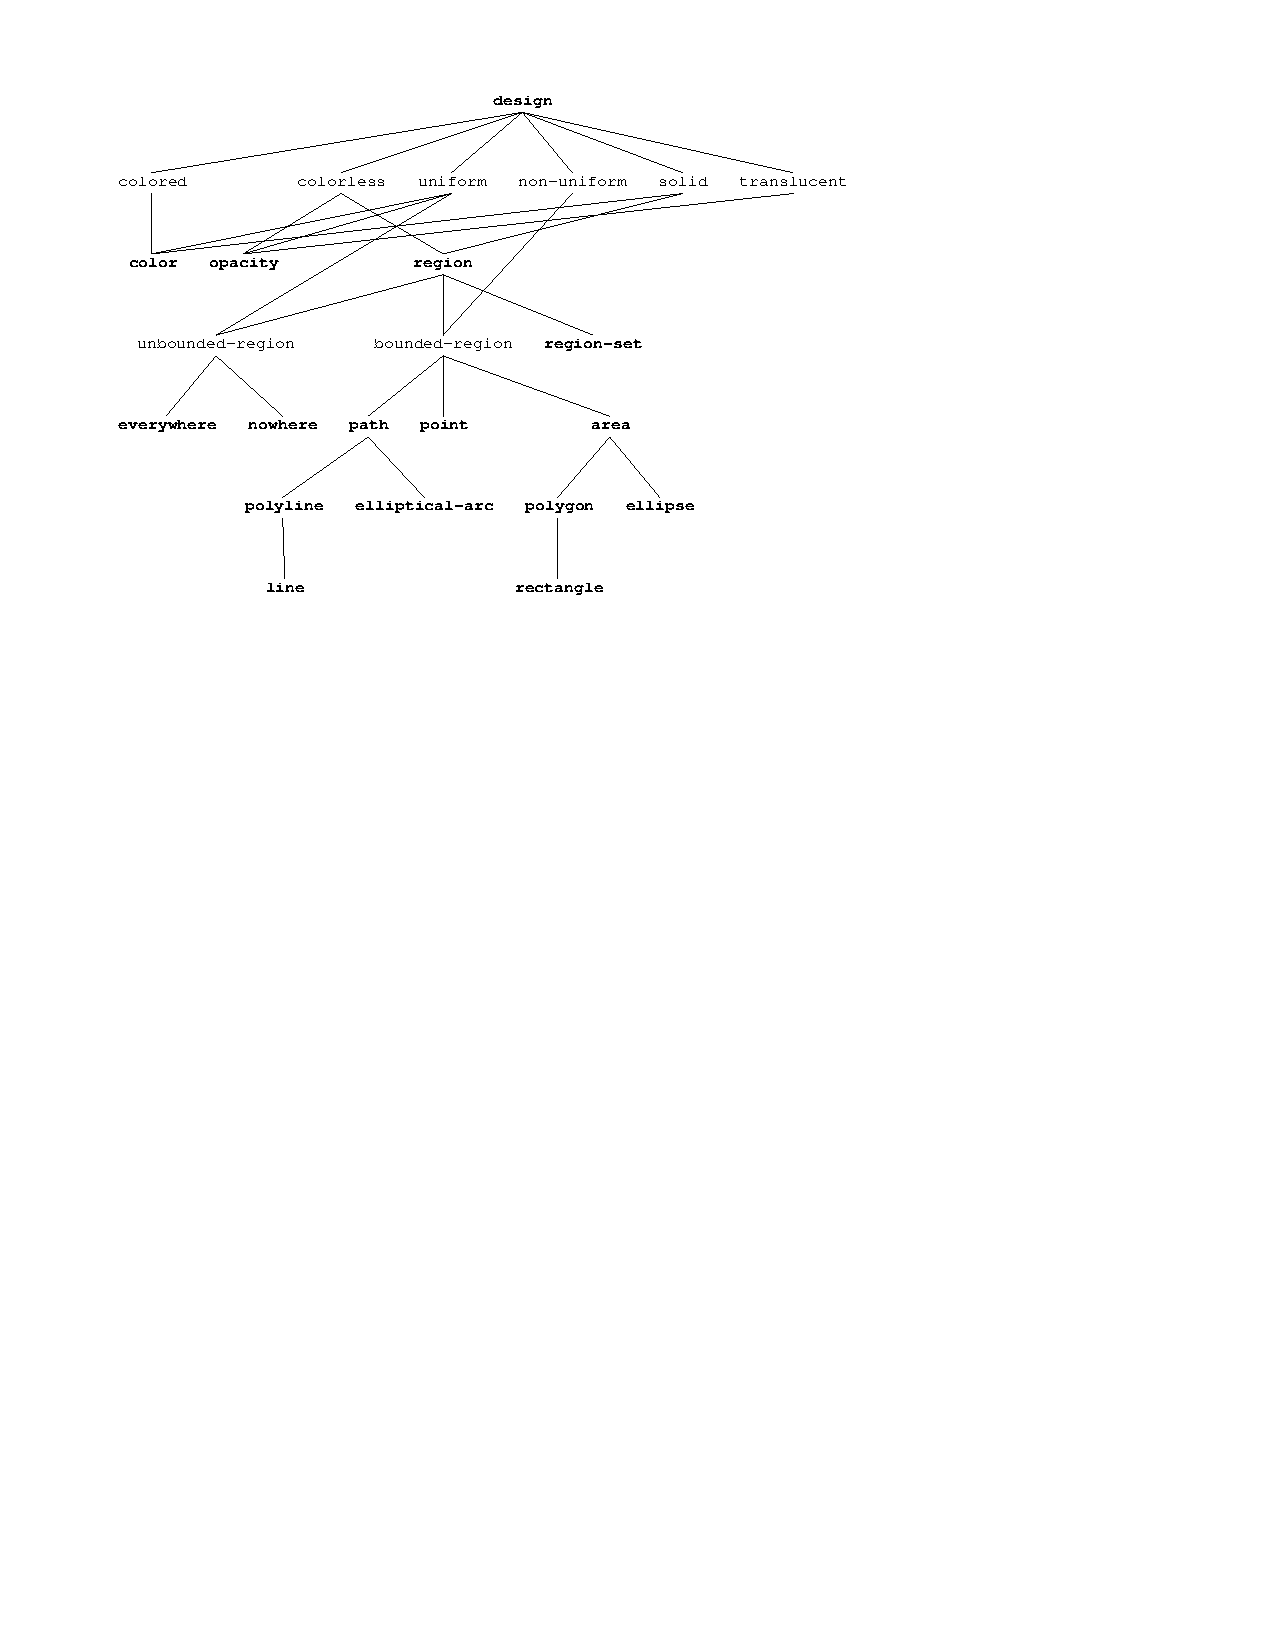
\includegraphics{design-classes}}
\caption{\label{design-classes} The class structure for all designs and regions.
Entries in bold correspond to real CLIM classes.}
\end{figure}

\issue {PM} {render via graphviz to remove overlapping edges?}

Since bounded designs obey the region protocol, the functions
\cl{transform-region} and \cl{untransform-region} accept any design as their
second argument and apply a coordinate transformation to the design.  The result
is a design that might be freshly constructed or might be an existing object.

Transforming a uniform design simply returns the argument.  Transforming a
composite, flipping, or indirect design applies the transformation to the
component design(s).  Transforming a pattern, tile, or output record design is
described in the sections on those designs.


\section {Arbitrary Designs}

\Defgeneric {draw-design} {medium design \key \DrawingOptions \LineJointCapOptions\ \TextOptions}

Draws the \term{design} \arg{design} onto the \term{medium} \arg{medium}.  This is
defined to work for all types of regions and designs, although in practice some
implementations may be more restrictive.  \arg{ink}, \arg{transformation}, and
\arg{clipping-region} are used to modify the medium.  The other drawing
arguments control the drawing of the design, depending on what sort of design is
being drawn.  For instance, if \arg{design} is a path, then line style options
may be supplied.

If \arg{design} is an area, \cl{draw-design} paints the specified region of the
drawing plane with medium's current ink.  If \arg{design} is a
path, \cl{draw-design} strokes the path with medium's current ink under control
of the line-style.  If \arg{design} is a point, \cl{draw-design} is the same as
\cl{draw-point}.

If \arg{design} is a color or an opacity, \cl{draw-design} paints the entire
drawing plane (subject to the clipping region of the medium).

If \arg{design} is \cl{+nowhere+}, \cl{draw-design} has no effect.

If \arg{design} is a non-uniform design (see Chapter~\ref{designs}),
\cl{draw-design} paints the design, positioned at coordinates $(0,0)$.

CLIM implementations are required to support \cl{draw-design} for the following
cases:

\begin{itemize}
\item Designs created by the geometric object constructors, such as
\cl{make-line} and \cl{make-ellipse}, in conjunction with drawing arguments that
supply the drawing ink.

\item Designs created by calling \cl{compose-in} on a color and an object
created by a geometric object constructor.

\item Designs created by calling \cl{compose-over} on any of the cases above.

\item Designs returned by \cl{make-design-from-output-record}.
\end{itemize}


\Defun {draw-pattern*} {medium pattern x y \key clipping-region transformation}

Draws the pattern \arg{pattern} on the \term{medium} \arg{medium} at the
position $(x,y)$. \arg{pattern} is any design created by \cl{make-pattern}.
\arg{clipping-region} and \arg{transformation} are as for
\cl{with-drawing-options} or any of the drawing functions.

Note that \arg{transformation} only affects the position at which the pattern is
drawn, not the pattern itself.  If a programmer wishes to affect the pattern, he
should explicity call \cl{transform-region} on the pattern.

Drawing a bitmap consists of drawing an appropriately aligned and scaled pattern
constructed from the bitmap's bits.  A 1 in the bitmap corresponds to
\cl{+foreground-ink+}, while a 0 corresponds to \cl{+background-ink+} if an
opaque drawing operation is desired, or to \cl{+nowhere+} if a transparent
drawing operation is desired.

Drawing a (colored) raster image consists of drawing an appropriately aligned
and scaled pattern constructed from the raster array and raster color map.

\cl{draw-pattern*} could be implemented as follows, assuming that the functions
\cl{pattern-width} and \cl{pattern-height} return the width and height of the
pattern.

\begin{verbatim}
(defun draw-pattern* (medium pattern x y &key clipping-region transformation)
  (check-type pattern pattern)
  (let ((width (pattern-width pattern))
        (height (pattern-height pattern)))
    (if (or clipping-region transformation)
        (with-drawing-options (medium :clipping-region clipping-region
                                      :transformation transformation)
          (draw-rectangle* medium x y (+ x width) (+ y height)
                           :filled t :ink pattern))
        (draw-rectangle* medium x y (+ x width) (+ y height)
                         :filled t :ink pattern))))
\end{verbatim}


\section {Examples of More Complex Drawing Effects}

\paragraph {Painting a gray or colored wash over a display.}

Specify a translucent design as the ink, such as \cl{:ink (compose-in +black+
(make-opacity 0.25))}, \cl{:ink (compose-in +red+ (make-opacity 0.1))}, or
\cl{:ink (compose-in +foreground-ink+ (make-opacity 0.75))}.  The last example
can be abbreviated as \cl{:ink (make-opacity 0.75)}.  On a non-color,
non-grayscale display this will usually turn into a stipple.

\paragraph {Drawing a faded but opaque version of the foreground color.}

Specify \cl{:ink (compose-over (compose-in +foreground-ink+ (make-opacity 0.25))
+background-ink+)} to draw at 25\% of the normal contrast.  On a non-color,
non-grayscale display this will probably turn into a stipple.

\paragraph {Drawing a tiled pattern.}

Specify \cl{:ink (make-rectangular-tile (make-pattern \arg{array} \arg{colors}))}.

\paragraph {Drawing a ``bitmap''.}

Use \cl{(draw-design \arg{medium} (make-pattern \arg{bit-array} (list
+background-ink+ +foreground-ink+)) :transformation
(make-translation-transformation \arg{x} \arg{y}))}.


\section {Design Protocol}

\issue {SWM} {The generic functions underlying the functions described in this
and the preceding chapter will be documented later.  This will allow for
programmer-defined design classes.  This also needs to describe how to decode
designs into inks.}


\part{Extended Stream Output Facilities}
% -*- Mode: LaTeX; Package: CLIM-USER -*-

\chapter {Extended Stream Output}
\label {extended-output}

CLIM provides a stream-oriented output layer that is implemented on top of the
sheet output architecture.  The basic CLIM output stream protocol is based on
the character output stream protocol proposal submitted to the ANSI Common Lisp
committee by David Gray.  This proposal was not approved by the committee, but
has been implemented by most Lisp vendors.

\section {Basic Output Streams}

CLIM provides an implementation of the basic output stream facilities (described
in more detail in Appendix~\ref{gray-streams}), either by directly using the
underlying Lisp implementation, or by implementing the facilities itself.

\Defclass {standard-output-stream}

This class provides an implementation of the CLIM basic output stream protocol,
based on the CLIM output kernel.
\Mutable

\Defgeneric {stream-write-char} {stream character}

Writes the character \arg{character} to the \term{output stream} \arg{stream},
and returns \arg{character} as its value.

\Defgeneric {stream-write-string} {stream string \optional (start \cl{0}) end}

Writes the string \arg{string} to the \term{output stream} \arg{stream}.  If
\arg{start} and \arg{end} are supplied, they are integers that specify what part
of \arg{string} to output.  \arg{string} is returned as the value.

\Defgeneric {stream-terpri} {stream}

Writes an end of line character on the \term{output stream} \arg{stream}, and
returns \term{false}.

\Defgeneric {stream-fresh-line} {stream}

Writes an end of line character on the \term{output stream} \arg{stream} only if
the stream is not at the beginning of the line.

\Defgeneric {stream-finish-output} {stream}

Ensures that all the output sent to the \term{output stream} \arg{stream} has
reached its destination, and only then return \term{false}.

\Defgeneric {stream-force-output} {stream}

Like \cl{stream-finish-output}, except that it may immediately return
\term{false} without waiting for the output to complete.

\Defgeneric {stream-clear-output} {stream}

Aborts any outstanding output operation in progress on the \term{output stream}
\arg{stream}, and returns \term{false}.

\Defgeneric {stream-line-column} {stream}

This function returns the column number where the next character will be written
on the \term{output stream} \arg{stream}.  The first column on a line is
numbered 0.

\Defgeneric {stream-start-line-p} {stream}

Returns \term{true} if the \term{output stream} \arg{stream} is positioned at
the beginning of a line (that is, column 0), otherwise returns \term{false}.

\Defgeneric {stream-advance-to-column} {stream column}

Writes enough blank space on the \term{output stream} \arg{stream} so that the
next character will be written at the position specified by \arg{column}, which
is an integer.


\section {Extended Output Streams}

In addition to the basic output stream protocol, CLIM defines an extended output
stream protocol.  This protocol extends the stream model to maintain the state
of a text cursor, margins, text styles, inter-line spacing, and so forth.

\Defprotoclass {extended-output-stream}

The protocol class for CLIM extended output streams.  This is a subclass of
\cl{output-stream}.
\IfYouWantClass {an} {extended output stream} {extended-output-stream}

\Defpredicate {extended-output-stream-p} {object}

Returns \term{true} if \arg{object} is a CLIM \term{extended output stream},
otherwise returns \term{false}.

\definitarg {:foreground}
\definitarg {:background}
\definitarg {:text-style}
\definitarg {:vertical-spacing}
\definitarg {:text-margin}
\definitarg {:end-of-line-action}
\definitarg {:end-of-page-action}
\Definitarg {:default-view}

All subclasses of \cl{extended-output-stream} must handle these initargs, which
are used to specify, respectively, the medium foreground and background, default
text style, vertical spacing, default text margin, end of line and end of page
actions, and the default view for the stream.

\cl{:foreground}, \cl{:background}, and \cl{:text-style} are handled via the
usual pane initialize options (see Section~\ref{pane-init}).

\Defclass {standard-extended-output-stream}

This class provides an implementation of the CLIM extended output stream
protocol, based on the CLIM output kernel.

\Mutable


\section {The Text Cursor}

In the days when display devices displayed only two dimensional arrays of fixed
width characters, the text cursor was a simple thing.  A discrete position was
selected in integer character units, and a character could go there and noplace
else.  Even for variable width fonts, simply addressing a character by the pixel
position of one of its corners is sufficient.  However, variable height fonts
with variable baselines on pixel-addressable displays upset this simple model.
The ``logical'' vertical reference point is the baseline, as it is in
typesetting.  In typesetting, however, an entire line of text is created with
baselines aligned and padded to the maximum ascent and descent, then the entire
line is put below the previous line.  

It is clearly desirable to have the characters on a line aligned with their
baselines, but when the line on the display is formed piece by piece, it is
impossible to pick in advance the proper baseline.  The solution CLIM adopts is
to choose a baseline, but not commit to it.

The CLIM model says that text has at least 6 properties.  With a reference point
of $(0,0)$ at the upper left of the text, it has a bounding box consisting of
ascent, descent, left kerning, right extension, and a displacement to the next
reference point in both $x$ and $y$.  CLIM determines the position of the
reference point and draws the text relative to that, and then the cursor
position is adjusted by the displacement.  In this way, text has width and
height, but the $x$ and $y$ displacements need not equal the width and height.

CLIM adopts the following approach to the actual rendering of a glyph.  Textual
output using the stream functions ({\sl not} the graphics functions) maintains
text on a ``line''.   Note that a line is not an output record, but is rather a
collection of ``text so far'', a top (which is positioned at the bottom of the
previous line plus the stream's vertical spacing), a baseline, a bottom, and a
``cursor position''.  The cursor position is defined to be at the top of the
line, not at the baseline.  The reason for this is that the baseline can move,
but the top is relative to the previous line, which has been completed and
therefore doesn't move.  If text is drawn on the current line whose ascent is
greater than the current ascent of the line, then the line is moved down to make
room.  This can be done easily using the output records for the existing text on
the line.  When there is enough room, the reference point for the text is the
$x$ position of the cursor at the baseline, and the cursor position is adjusted
by the displacement.

The following figures show this in action before and after each of three
characters are drawn.  In all three figure, the small circle is the ``cursor
position''.  At first, there is nothing on the line.  The first character
establishes the initial baseline, and is then drawn.  The upper left corner of
the character is where the cursor was (as in the traditional model), but this
will not remain the case.  Drawing the second character, which is larger than
the first, requires moving the first character down in order to get the
baselines to align; during this time, the top of the line remains the same.
Again, the upper left of the second character is where the cursor was, but that
is no longer the case for the first character (which has moved down).  The third
character is smaller than the second, so no moving of characters needs to be
done.  However, the character is drawn to align the baselines, which in this
case means the upper left is {\sl not} where the cursor was.  Nor is the cursor
at the upper right of the character as it was for the previous two characters.
It is, however, at the upper right of the collective line.

{
\setlength\unitlength{.1in}
\def\NoChars{
        \begin{picture}(10,30)(0,-20)
        \put(0,0){\line(1,0){4}}
        \put(-2,2){\makebox(0,0)[r]{(0,y)}}
        \put(-2,2){\vector(1,-1){2}}
        \put(0,0){\circle*{.5}}
        \end{picture}
        }
\def\OneChar{
        \begin{picture}(10,30)(0,-20)
        \put(0,0){\line(1,0){12}}
        \put(-2,2){\makebox(0,0)[r]{(0,y)}}
        \put(-2,2){\vector(1,-1){2}}
        \put(0,-12){\framebox(8,12){small}}
        \put(4,4){\makebox(0,0)[r]{(w1,y)}}
        \put(4,4){\vector(1,-1){4}}
        \put(8,0){\circle*{.5}}
        \put(-2,-16){\makebox(0,0)[r]{bl-small}}
        \put(-2,-16){\vector(1,3){2}}
        \put(0,-10){\vector(1,0){10}}
        \end{picture}
        }
\def\TwoChars{
        \begin{picture}(10,30)(0,-20)
        \put(0,0){\line(1,0){22}}
        \put(-2,2){\makebox(0,0)[r]{(0,y)}}
        \put(-2,2){\vector(1,-1){2}}
        \put(0,-14){\framebox(8,12){small}}
        \put(4,4){\makebox(0,0)[r]{(w1,y)}}
        \put(4,4){\vector(1,-1){4}}
        \put(8,-16){\framebox(10,16){BIG}}
        \put(12,6){\makebox(0,0)[r]{(w1+w2,y)}}
        \put(12,6){\vector(1,-1){6}}
        \put(18,0){\circle*{.5}}
        \put(-2,-18){\makebox(0,0)[r]{bl-BIG}}
        \put(-2,-18){\vector(1,3){2}}
        \put(0,-12){\vector(1,0){20}}
        \end{picture}
        }
\def\ThreeChars{
        \begin{picture}(10,30)(0,-20)
        \put(0,0){\line(1,0){30}}
        \put(-2,2){\makebox(0,0)[r]{(0,y)}}
        \put(-2,2){\vector(1,-1){2}}
        \put(0,-14){\framebox(8,12){small}}
        \put(4,4){\makebox(0,0)[r]{(w1,y)}}
        \put(4,4){\vector(1,-1){4}}
        \put(8,-16){\framebox(10,16){BIG}}
        \put(12,6){\makebox(0,0)[r]{(w1+w2,y)}}
        \put(12,6){\vector(1,-1){6}}
        \put(18,-14){\framebox(8,12){small}}
        \put(18,8){\makebox(0,0)[r]{(w1+w2+w3,y)}}
        \put(18,8){\vector(1,-1){8}}
        \put(26,0){\circle*{.5}}
        \put(-2,-18){\makebox(0,0)[r]{bl-BIG}}
        \put(-2,-18){\vector(1,3){2}}
        \put(0,-12){\vector(1,0){28}}
        \end{picture}
        }

\begin{picture}(50,60)(-4,0)
        \put(0,30){\NoChars}
        \put(10,30){\OneChar}
        \put(30,30){\TwoChars}
        \put(10,0){\ThreeChars}
\end{picture}

}

\issue {DCPL} {The above may be too simplistic. The displacement probably
wants to depend not only on language but language rendering mode.  For example,
Japanese can apparently go either vertically or horizontally.  It may be
necessary to have the bounding box and perhaps the reference point dispatch as
well.  Similarly, ``newline'' could mean ``down one line, all the way to the
left'' for English, ``down one line, all the way to the right'' for Arabic, or
``to the left one line, all the way to the top.''  ``Home cursor'' is another
ditty to consider.  We need to discuss this on a larger scale with people who
know multi-lingual rendering issues.}


\subsection {Text Cursor Protocol}

Many streams that maintain a text cursor display some visible indication of the
text cursor.  The object that represents this display is (somewhat confusingly)
also called a cursor.

An \concept{active} cursor is one that is being actively maintained by its
owning sheet.  A active cursor has a \concept{state} that is either on or off.
An active cursor can also has a state that indicates the the owning sheet has
the input focus.

\Defprotoclass {cursor}

The protocol class that corresponds to cursors.
\IfYouWantClass {a} {cursor} {cursor}
\Mutable

\Defpredicate {cursorp} {object}

Returns \term{true} if \arg{object} is a \term{cursor}, otherwise returns
\term{false}.

\Definitarg {:sheet}

The \cl{:sheet} initarg is used to specify the sheet with which the cursor is
associated.

\Defclass {standard-text-cursor}

The instantiable class that implements a text cursor.  Typically, ports will
further specialize this class.

\Defgeneric {cursor-sheet} {cursor}

Returns the sheet with which the \term{cursor} \arg{cursor} is associated.

\Defgeneric {cursor-position} {cursor}

Returns the $x$ and $y$ position of the \term{cursor} \arg{cursor} as two
values.  $x$ and $y$ are in the coordinate system of the cursor's sheet.

\Defgeneric {(setf* cursor-position)} {x y cursor}

Sets the $x$ and $y$ position of the \term{cursor} \arg{cursor} to the specified
position.  $x$ and $y$ are in the coordinate system of the cursor's sheet.

For CLIM implementations that do not support \cl{setf*}, the ``setter'' function
for this is \cl{cursor-set-position}.

\defgeneric {cursor-active} {cursor}
\Defgeneric {(setf cursor-active)} {value cursor}

Returns (or sets) the ``active'' attribute of the cursor.  When \term{true}, the
cursor is active.

\defgeneric {cursor-state} {cursor}
\Defgeneric {(setf cursor-state)} {value cursor}

Returns (or sets) the ``state'' attribute of the cursor.  When \term{true}, the
cursor is visible.  When \term{false}, the cursor is not visible.

\Defgeneric {cursor-focus} {cursor}

Returns the ``focus'' attribute of the cursor.  When \term{true}, the sheet
owning the cursor has the input focus.

\defgeneric {cursor-visibility} {cursor}
\Defgeneric {(setf cursor-visibility)} {visibility cursor}

These are convenience functions that combine the functionality of
\cl{cursor-active} and \cl{cursor-state}.  The visibility can be either \cl{:on}
(meaning that the cursor is active and visible at its current position),
\cl{:off} (meaning that the cursor is active, but not visible at its current
position), or \cl{nil} (meaning that the cursor is not activate).


\subsection {Stream Text Cursor Protocol}

The following generic functions comprise the stream text cursor protocol.  Any
extended output stream class must implement methods for these generic functions.

\Defgeneric {stream-text-cursor} {stream}
\Defgeneric {(setf stream-text-cursor)} {cursor stream}

Returns (or sets) the text cursor object for the stream \arg{stream}.


\Defgeneric {stream-cursor-position} {stream}

Returns the current text cursor position for the \term{extended output stream}
\arg{stream} as two integer values, the $x$ and $y$ positions.

\Defgeneric {(setf* stream-cursor-position)} {x y stream}

Sets the text cursor position of the \term{extended output stream} \arg{stream}
to \arg{x} and \arg{y}.  \arg{x} and \arg{y} are in device units, and must be
integers.

For CLIM implementations that do not support \cl{setf*}, the ``setter'' function
for this is \cl{stream-set-cursor-position}.

\Defgeneric {stream-increment-cursor-position} {stream dx dy}

Moves the text cursor position of the \term{extended output stream} \arg{stream}
relatively, adding \arg{dx} to the $x$ coordinate and \arg{dy} to the $y$
coordinate.  Either of \arg{dx} or \arg{dy} may be \cl{nil}, meaning the the $x$
or $y$ cursor position will be unaffected.  Otherwise, \arg{dx} and \arg{dy}
must be integers.


\section {Text Protocol}

The following generic functions comprise the text protocol.  Any extended output
stream class must implement methods for these generic functions.

\Defgeneric {stream-character-width} {stream character \key text-style}

Returns a rational number corresponding to the amount of horizontal motion of
the cursor position that would occur if the character \arg{character} were
output to the \term{extended output stream} \arg{stream} in the \term{text
style} \arg{text-style} (which defaults to the current text style for the
stream).  This ignores the stream's text margin.

\Defgeneric {stream-string-width} {stream character \key start end text-style}

Computes how the cursor position would move horizontally if the string
\arg{string} were output to the \term{extended output stream} \arg{stream} in
the \term{text style} \arg{text-style} (which defaults to the current text style
for the stream) starting at the left margin.  This ignores the stream's text
margin.

The first returned value is the $x$ coordinate that the cursor position would
move to.  The second returned value is the maximum $x$ coordinate the cursor
would visit during the output. (This is the same as the first value unless the
string contains a \verb+#\Newline+ character.)

\arg{start} and \arg{end} are integers, and default to 0 and the length of the
string, respectively.


\defgeneric {stream-text-margin} {stream}
\Defgeneric {(setf stream-text-margin)} {margin stream}

The $x$ coordinate at which text wraps around on the \term{extended output
stream} \arg{stream} (see \cl{stream-end-of-line-action}).  The default setting
is the width of the viewport, which is the right-hand edge of the viewport when
it is horizontally scrolled to the ``initial position''.

You can use \cl{setf} with \cl{stream-text-margin} to establish a new text
margin.  If \arg{margin} is \cl{nil}, then the width of the viewport will be
used.  If the width of the viewport is later changed, the text margin will
change, too.


\Defgeneric {stream-line-height} {stream \key text-style}

Returns what the line height of a line on the \term{extended output stream}
\arg{stream} containing text in the \term{text style} \arg{text-style} would be,
as a rational number.  The height of the line is measured from the baseline of
the text style to its ascent.  \arg{text-style} defaults to the current text
style for the stream.


\Defgeneric {stream-vertical-spacing} {stream}

Returns the current inter-line spacing (as a rational number) for the
\term{extended output stream} \arg{stream}.

\Defgeneric {stream-baseline} {stream}

Returns the current text baseline (as a rational number) for the \term{extended
output stream} \arg{stream}.


\subsection {Mixing Text and Graphics}

The following macro provides a convenient way to mix text and graphics on the
same output stream.

\Defmacro {with-room-for-graphics} {(\optional stream
                                     \key (first-quadrant \cl{t}) height (move-cursor \cl{t})
                                          record-type)
                                    \body body}

Binds the dynamic environment to establish a local coordinate system for doing
graphics output onto the \term{extended output stream} designated by
\arg{stream}.  If \arg{first-quadrant} is \term{true} (the default), a local
Cartesian coordinate system is established with the origin $(0,0)$ of the local
coordinate system placed at the current cursor position; $(0,0)$ is in the lower
left corner of the area created.  If the boolean \arg{move-cursor} is
\term{true} (the default), then after the graphic output is completed, the
cursor is positioned past (immediately below) this origin.  The bottom of the
vertical block allocated is at this location (that is, just below point $(0,0)$,
not necessarily at the bottom of the output done).

The \arg{stream} argument is not evaluated, and must be a symbol that is bound
to a stream.  If \arg{stream} is \cl{t} (the default), \cl{*standard-output*} is
used.  \arg{body} may have zero or more declarations as its first forms.

If \arg{height} is supplied, it must be a rational number that specifies the
amount of vertical space to allocate for the output, in device units. If it is
not supplied, the height is computed from the output.

\arg{record-type} specifies the class of output record to create to hold the
graphical output.  The default is \cl{standard-sequence-output-record}.


\subsection {Wrapping of Text Lines}

\defgeneric {stream-end-of-line-action} {stream}
\Defgeneric {(setf stream-end-of-line-action)} {action stream}

The end-of-line action controls what happens if the text cursor position moves
horizontally out of the viewport, or if text output reaches the text margin.
(By default the text margin is the width of the viewport, so these are usually
the same thing.)

\cl{stream-end-of-line-action} returns the end-of-line action for the
\term{extended output stream} \arg{stream}.  It can be changed by using
\cl{setf} on \cl{stream-end-of-line-action}.

The end-of-line action is one of: 

\begin{itemize}
\item \cl{:wrap}---when doing text output, wrap the text around (that is, break
the text line and start another line).  When setting the cursor position, scroll
the window horizontally to keep the cursor position inside the viewport.  This
is the default.

\item \cl{:scroll}---scroll the window horizontally to keep the cursor
position inside the viewport, then keep doing the output.

\item \cl{:allow}---ignore the text margin and do the output on the drawing
plane beyond the visible part of the viewport.
\end{itemize}

\Defmacro {with-end-of-line-action} {(stream action) \body body}

Temporarily changes \arg{stream}'s end-of-line action for the duration of
execution of body.  \arg{action} must be one of the actions described in
\cl{stream-end-of-line-action}.

The \arg{stream} argument is not evaluated, and must be a symbol that is bound
to a stream.  If \arg{stream} is \cl{t}, \cl{*standard-output*} is used.
\arg{body} may have zero or more declarations as its first forms.


\defgeneric {stream-end-of-page-action} {stream}
\Defgeneric {(setf stream-end-of-page-action)} {action stream}

The end-of-page action controls what happens if the text cursor position moves
vertically out of the viewport.

\cl{stream-end-of-page-action} returns the end-of-page action for the
\term{extended output stream} \arg{stream}.  It can be changed by using
\cl{setf} on \cl{stream-end-of-page-action}.

The end-of-page action is one of: 

\begin{itemize}
\item \cl{:scroll}---scroll the window vertically to keep the cursor position
inside the viewport, then keep doing output.  This is the default.

\item \cl{:allow}---ignore the viewport and do the output on the drawing plane
beyond the visible part of the viewport.

\item \cl{:wrap}---when doing text output, wrap the text around (that is, go back
to the top of the viewport).
\end{itemize}

\Defmacro {with-end-of-page-action} {(stream action) \body body}

Temporarily changes \arg{stream}'s end-of-page action for the duration of
execution of body.  \arg{action} must be one of the actions described in
\cl{stream-end-of-page-action}.

The \arg{stream} argument is not evaluated, and must be a symbol that is bound
to a stream.  If \arg{stream} is \cl{t}, \cl{*standard-output*} is used.
\arg{body} may have zero or more declarations as its first forms.


\section {Attracting the User's Attention}

\Defgeneric {beep} {\optional medium}

Attracts the user's attention, usually with an audible sound.


\section {Buffering of Output}

Some mediums that support the output protocol may buffer output.  When buffering
is enabled on a medium, the time at which output is actually done on the medium
is unpredictable.  \cl{force-output} or \cl{finish-output} can be used to ensure
that all pending output gets completed.  If the medium is a bidirectional
stream, a \cl{force-output} is performed whenever any sort of input is requested
on the stream.

\cl{with-buffered-output} provides a way to control when buffering is enabled on
a medium.  By default, CLIM's interactive streams are buffered if the underlying
window system supports buffering.

\Defgeneric {medium-buffering-output-p} {medium}

Returns \term{true} if the \term{medium} \arg{medium} is currently buffering
output, otherwise returns \term{false}.

\Defgeneric {(setf medium-buffering-output-p)} {buffer-p medium}

Sets \cl{medium-buffering-output-p} of the \term{medium} \arg{medium} to
\arg{buffer-p}.

\Defmacro {with-output-buffered} {(medium \optional (buffer-p \cl{t}))
                                  \body body}

If \arg{buffer-p} is \term{true} (the default), this causes the \term{medium}
designated by \arg{medium} to start buffering output, and evaluates \arg{body}
in that context.  If \arg{buffer-p} is \term{false}, \cl{force-output} will be
called before \arg{body} is evaluated.  When \arg{body} is exited (or aborted
from), \cl{force-output} will be called if output buffering will be disabled
after \cl{with-output-buffered} is exited.

The \arg{medium} argument is not evaluated, and must be a symbol that is bound
to a medium.  If \arg{medium} is \cl{t}, \cl{*standard-output*} is used.
\arg{body} may have zero or more declarations as its first forms.

% -*- Mode: LaTeX; Package: CLIM-USER -*-

\chapter {Output Recording}
\label {output-recording}

\section {Overview of Output Recording}

CLIM provides a mechanism whereby output (textual and graphical) may be captured
into an \concept{output history} for later replay on the same stream.  This
mechanism serves as the basis for many other tools, such as the formatted output
and presentation mechanisms described elsewhere.

The output recording facility is layered on top of the graphics and text output
protocols.  It works by intercepting the operations in the graphics and text
output protocols, and saving information about these operations in objects
called \concept{output records}.  In general, an output record is a kind of
display list, that is, a collection of instructions for drawing something on a
stream.  Some output records may have \concept{children}, that is, a collection
of inferior output records.  Other output records, which are called
\concept{displayed output records}, correspond directly to displayed information
on the stream, and do not have children.  If you think of output records being
arranged in a tree, displayed output records are all of the leaf nodes in the
tree, for example, displayed text and graphics records.

Displayed output records must record the state of the supplied drawing options
at the instant the output record is created, as follows.  The ink supplied by
the programmer must be captured without resolving indirect inks; this is so that
a user can later change the default foreground and background ink of the medium
and have that change affect the already-created output records during replay.
The effect of the specified ``user'' transformation (composed with the medium
transformation) must be captured; CLIM implementations are free to do this
either by saving the transformation object or by saving the transformed values
of all objects that are affected by the transformation.  The user clipping
region and line style must be captured in the output record as well.  Subsequent
replaying of the record under a new user transformation, clipping region, or
line style will not affect the replayed output.  CLIM implementation are
permitted to capture the text style either fully merged against the medium's
default, or not; in the former case, subsequent changes to the medium's default
text style will not affect replaying the record, but in the latter case changing
the default text style will affect replaying.

A CLIM stream that supports output recording has an output history object, which
is a special kind of output record that supports some other operations.  CLIM
defines a standard set of output history implementations and a standard set of
output record types.

The output recording mechanism is defined so as to permit application specific
or host window system specific implementations of the various recording
protocols.  CLIM implementations should provide several types of standard output
records with different characteristics for search, storage, and retrieval.  Two
examples are ``sequence'' output records (which store elements in a sequence,
and whose insertion and retrieval complexity is O(n)) and ``tree'' output
records (which store elements in some sort of tree based on the location of the
element, and whose insertion and retrieval complexity is O(log~n)).

\Issue {York, SWM} {There is a proposal on the table to unify the sheet and
output record protocols, not by unifying the class structure, but by making them
implement the same generic functions where that makes sense.  For instance,
sheets and output records both have regions, transformations (that relate sheets
to their parents), both support a repainting operation, and so forth.

In particular, \cl{sheet-parent} and \cl{output-record-parent} are equivalent,
as are \cl{sheet-children} and \cl{output-record-children},
\cl{sheet-adopt-child} and \cl{add-output-record}, \cl{sheet-disown-child} and
\cl{delete-output-record}, and \cl{repaint-sheet} and \cl{replay-output-record},
and the mapping functions.  \cl{output-record-position} and its \cl{setf}
function have sheet analogs.  The sheet and output record notification functions
are also equivalent.

This simplifies the conceptual framework of CLIM, and could eventually simplify
the implementation as well.  Doing this work now opens the door for later
unifications, such unifying the pane layout functionality with table formatting.}


\section {Output Records}

\Defprotoclass {output-record}

The protocol class that is used to indicate that an object is an output record,
that is, an object that contains other output records.  This is a subclass of
\cl{bounding-rectangle}, and as such, output records obey the bounding rectangle
protocol.
\IfYouWantClass {an} {output record} {output-record}

All output records are mutable.

\Defpredicate {output-record-p} {object}

Returns \term{true} if \arg{object} is an \term{output record}, otherwise
returns \term{false}.

\Defprotoclass {displayed-output-record}

The protocol class that is used to indicate that an object is a displayed output
record, that is, an object that represents a visible piece of output on
some output stream.  This is a subclass of \cl{bounding-rectangle}.
\IfYouWantClass {a} {displayed output record} {displayed-output-record}

All displayed output records are mutable.

\Defpredicate {displayed-output-record-p} {object}

Returns \term{true} if \arg{object} is a \term{displayed output record},
otherwise returns \term{false}.

\definitarg {:x-position}
\definitarg {:y-position}
\Definitarg {:parent}

All subclasses of either \cl{output-record} or \cl{displayed-output-record} must
handle these three initargs, which are used to specify, respectively, the $x$
and $y$ position of the output record, and the parent of the output record.

\Definitarg {:size}

All subclasses of \cl{output-record} must handle the \cl{:size} initarg.  It is
used to specify how much room should be left for child output records (if, for
example, the children are stored in a vector).  It is permissible for \cl{:size}
to be ignored, provided that the resulting output record is able to store the
specified number of child output records.


\subsection {The Basic Output Record Protocol}

All subclasses of \cl{output-record} and \cl{displayed-output-record} must
inherit or implement methods for the following generic functions.

When the generic functions in this section take both \arg{record} and a
\arg{stream} arguments, CLIM implementations will specialize the \arg{stream}
argument for the \cl{standard-output-recording-stream} class and the
\arg{record} argument for all of the implementation-specific output record
classes.

\Defgeneric {output-record-position} {record}

Returns the $x$ and $y$ position of the \term{output record} \arg{record} as two
rational numbers.  The position of an output record is the position of the
upper-left corner of its bounding rectangle.  The position is relative to the
stream, where $(0,0)$ is (initially) the upper-left corner of the stream.

\Defgeneric {(setf* output-record-position)} {x y record}

Changes the $x$ and $y$ position of the \term{output record} \arg{record} to be
\arg{x} and \arg{y} (which are rational numbers), and updates the bounding
rectangle to reflect the new position (and saved cursor positions, if the output
record stores it).  If \arg{record} has any children, all of the children (and
their descendants as well) will be moved by the same amount as \arg{record} was
moved.  The bounding rectangles of all of \arg{record}'s ancestors will also be
updated to be large enough to contain \arg{record}.  This does not replay the
output record, but the next time the output record is replayed it will appear at
the new position.

For CLIM implementations that do not support \cl{setf*}, the ``setter'' function
for this is \cl{output-record-set-position}.

\Defgeneric {output-record-start-cursor-position} {record}

Returns the $x$ and $y$ starting cursor position of the \term{output record}
\arg{record} as two integer values.  The positions are relative to the stream,
where $(0,0)$ is (initially) the upper-left corner of the stream.

Text output records and updating output records maintain the cursor position.
Graphical output records and other output records that do not require or affect
the cursor position will return \cl{nil} as both of the values.

\Defgeneric {(setf* output-record-start-cursor-position)} {x y record}

Changes the $x$ and $y$ starting cursor position of the \term{output record}
\arg{record} to be \arg{x} and \arg{y} (which are integers).  This does not
affect the bounding rectangle of \arg{record}, nor does it replay the output
record.  For those output records that do not require or affect the cursor
position, the method for this function is a no-op.

For CLIM implementations that do not support \cl{setf*}, the ``setter'' function
for this is \cl{output-record-set-start-cursor-position}.

\Defgeneric {output-record-end-cursor-position} {record}

Returns the $x$ and $y$ ending cursor position of the \term{output record}
\arg{record} as two integer values.  The positions are relative to the stream,
where $(0,0)$ is (initially) the upper-left corner of the stream.  Graphical
output records do not track the cursor position, so only text output record (and
some others) will return meaningful values for this.

Text output records and updating output records maintain the cursor position.
Graphical output records and other output records that do not require or affect
the cursor position will return \cl{nil} as both of the values.

\Defgeneric {(setf* output-record-end-cursor-position)} {x y record}

Changes the $x$ and $y$ ending cursor position of the \term{output record}
\arg{record} to be \arg{x} and \arg{y} (which are integers).  This does not
affect the bounding rectangle of \arg{record}, nor does it replay the output
record.  For those output records that do not require or affect the cursor
position, the method for this function is a no-op.

For CLIM implementations that do not support \cl{setf*}, the ``setter'' function
for this is \cl{output-record-set-end-cursor-position}.

\Defgeneric {output-record-parent} {record}

Returns the output record that is the parent of the \term{output record}
\arg{record}, or \cl{nil} if the record has no parent.


\Defun {replay} {record stream \optional region}

This function bind \cl{stream-recording-p} of \arg{stream} to \term{false}, and
then calls \cl{replay-output-record} on the arguments \arg{record},
\arg{stream}, and \arg{region}.  If \cl{stream-drawing-p} of \arg{stream} is
\term{false}, \cl{replay} does nothing.  \cl{replay} is typically called during
scrolling, by repaint handlers, and so on.

CLIM implementations are permitted to default \arg{region} either to \cl{nil} or
to the region corresponding to viewport of \arg{stream}.

\Defgeneric {replay-output-record} {record stream \optional region x-offset y-offset}

Displays the output captured by the \term{output record} \arg{record} on the
\term{output recording stream} \arg{stream}, exactly as it was originally
captured (subject to subsequent modifications).  The current user
transformation, line style, text style, ink, and clipping region of \arg{stream}
are all ignored during the replay operation.  Instead, these are gotten from the
output record.

If \arg{record} is not a displayed output record, then replaying it involves
replaying all of its children.  If \arg{record} is a displayed output record,
then replaying it involves redoing the graphics operation captured in the
record.

\arg{region} is a region that can be supplied to limit what records are
displayed.  Only those records that overlap \arg{region} are replayed.  The
default for \arg{region} is \cl{+everywhere+}.

It is permissible for implementations to restrict \cl{replay-output-record} such
that \arg{stream} must be the same stream on which the output records were
originally recorded.

\issue {SWM} {How does replaying a text output record (or any record that
maintains the cursor position) affect the cursor position of the stream?  It
is probably that case that \cl{replay} should not affect the cursor position.}


\Defgeneric {output-record-hit-detection-rectangle*} {record}

This method is used to establish the usual ``effective size'' of \arg{record}
for hit detection queries.  Four values are returned corresponding to the edges
of the bounding rectangle that is the hit detection rectangle.  The default
method (on CLIM's standard output record class) is equivalent to calling calling
\cl{bounding-rectangle*} on \arg{record}, but this method can be specialized to
return a larger bounding rectangle in order to implement a form of hysteresis.

\Defgeneric {output-record-refined-position-test} {record x y}

This is used to definitively answer hit detection queries, that is, determining
that the point $(x,y)$ is contained within the output record \arg{record}.  Once
the position $(x,y)$ has been determined to lie within
\cl{output-record-hit-detection-rectangle*},
\cl{output-record-refined-sensitivity-test} is invoked.  Output record
subclasses can provide a method that provides a more precise definition of a
hit, for example, output records for elliptical rings will implement a method
that detects whether the pointing device is on the elliptical ring.

\Defgeneric {highlight-output-record} {record stream state}

This method is called in order to draw a highlighting box around the
\term{output record} \arg{record} on the \term{output recording stream}
\arg{stream}.  \arg{state} will be either \cl{:highlight} (meaning to draw the
highlighting) or \cl{:unhighlight} (meaning to erase the highlighting).  The
default method (on CLIM's standard output record class) will simply draw a
rectangle that corresponds the the bounding rectangle of \arg{record}.

\Defgeneric {displayed-output-record-ink} {displayed-output-record}

Returns the ink used by the \term{displayed output record}
\arg{displayed-output-record}.


\subsection {The Output Record ``Database'' Protocol}

All classes that are subclasses of \cl{output-record} must implement methods for
the following generic functions.

\Defgeneric {output-record-children} {record}

Returns a sequence of all of the children of the \term{output record}
\arg{record}.  It is unspecified whether the sequence is a freshly created
object or a ``live'' object representing the state of \arg{record}.

\Defgeneric {add-output-record} {child record}

Adds the new \term{output record} \arg{child} to the \term{output record}
\arg{record}.  The bounding rectangle for \arg{record} (and all its ancestors)
must be updated to account for the new child record.

The methods for the \cl{add-output-record} will typically specialize only the
\arg{record} argument.

\Defgeneric {delete-output-record} {child record \optional (errorp \cl{t})}

Removes the \term{output record} \arg{child} from the \term{output record}
\arg{record}.  The bounding rectangle for \arg{record} (and all its ancestors)
may be updated to account for the child having been removed, although this is
not mandatory.

If \arg{errorp} is \term{true} (the default) and \arg{child} is not contained
within \arg{record}, then an error is signalled.

The methods for the \cl{delete-output-record} will typically specialize only the
\arg{record} argument.

\Defgeneric {clear-output-record} {record}

Removes all of the children from the \term{output record} \arg{record}, and
resets the bounding rectangle of \arg{record} to its initial state.

\Defgeneric {output-record-count} {record}

Returns the number of children contained within the \term{output record}
\arg{record}.


\Defgeneric {map-over-output-records-containing-position} 
            {function record x y \optional x-offset y-offset \rest function-args}

Maps over all of the children of the \term{output record} \arg{record} that
contain the point at $(x,y)$, calling \arg{function} on each one.
\arg{function} is a function of one or more arguments, the first argument being
the record containing the point; it has dynamic extent.  \arg{function} is also
called with all of \arg{function-args} as ``apply'' arguments.

If there are multiple records that contain the point and that overlap each
other, \cl{map-over-output-records-containing-position} must hit the uppermost
(most recently inserted) record first and the bottommost (least recently
inserted) record last.  Otherwise, the order in which the records are traversed
is unspecified.

\Defgeneric {map-over-output-records-overlapping-region}
            {function record region \optional x-offset y-offset \rest function-args}

Maps over all of the children of the \term{output record} \arg{record} that
overlap the \term{region} \arg{region}, calling \arg{function} on each one.
\arg{function} is a function of one or more arguments, the first argument being
the record overlapping the region; it has dynamic extent.  \arg{function} is
also called with all of \arg{function-args} as ``apply'' arguments.

If there are multiple records that overlap the region and that overlap each
other, \cl{map-over-output-records-overlapping-region} must hit the bottommost
(least recently inserted) record first and the uppermost (most recently
inserted) record last.  Otherwise, the order in which the records are traversed
is unspecified.


\subsection {Output Record Change Notification Protocol}

The following functions are called by programmers and by CLIM itself in order to
notify a parent output record when the bounding rectangle of one of its child output
record changes.

\Defgeneric {recompute-extent-for-new-child} {record child}

This function is called whenever a new child is added to an output record.  Its
contract is to update the bounding rectangle of the \term{output record}
\arg{record} to be large enough to completely contain the new child \term{output
record} \arg{child}. The parent of \arg{record} must be notified by calling
\cl{recompute-extent-for-changed-child}.

\cl{add-output-record} is required to call \cl{recompute-extent-for-new-child}.

\Defgeneric {recompute-extent-for-changed-child} {record child 
                                                  old-min-x old-min-y old-max-x old-max-y} 

This function is called whenever the bounding rectangle of one of the children of
a record has been changed.  Its contract is to update the bounding rectangle of
the \term{output record} \arg{record} to be large enough to completely contain
the new bounding rectangle of the child \term{output record} \arg{child}.  All
of the ancestors of \arg{record} must be notified by recursively calling
\cl{recompute-extent-for-changed-child}.

Whenever the bounding rectangle of an output record is changed or
\cl{delete-output-record} is called, \cl{recompute-extent-for-changed-child}
must be called to inform the parent of the record that a change has taken place.

\Defgeneric {tree-recompute-extent} {record}

This function is called whenever the bounding rectangles of a number of children
of a record have been changed, such as happens during table and graph
formatting.  Its contract is to compute the bounding rectangle large enough to
contain all of the children of the output record \arg{record}, adjust the
bounding rectangle of the \term{output record} \arg{record} accordingly, and
then call \cl{recompute-extent-for-changed-child} on \arg{record}.


\section {Types of Output Records}

This section discusses several types of output records, including two standard
classes of output records and the displayed output record protocol.

\subsection {Standard Output Record Classes}

\Defclass {standard-sequence-output-record}

The standard instantiable class provided by CLIM to store a relatively short
sequence of output records; a subclass of \cl{output-record}.  The insertion and
retrieval complexity of this class is O(n).  Most of the formatted output
facilities (such as \cl{formatting-table}) create output records that are a
subclass of \cl{standard-sequence-output-record}.

\Defclass {standard-tree-output-record}

The standard instantiable class provided by CLIM to store longer sequences of
output records.  Typically, the child records of a tree output record will be
maintained in some sort of sorted order, such as a lexicographic ordering on the
$x$ and $y$ coordinates of the children.  The insertion and retrieval complexity
of this class is O(log~n).


\subsection {Graphics Displayed Output Records}

Graphics displayed output records are used to record the output produced by the
graphics functions, such as \cl{draw-line*}.  Each graphics displayed output
record describes the output produced by a call to one of the graphics functions.

The exact contents of graphics displayed output records is unspecified, but they
must store sufficient information to be able to exactly redraw the original
output at replay time.  The minimum information that must be captured for
all graphics displayed output records is as follows:

\begin{itemize}
\item The description of the graphical object itself, for example, the end
points of a line or the center point and radius of a circle.

\item The programmer-supplied ink at the time the drawing function was called.
Indirect inks must not be resolved, so that a user can later change the default
foreground and background ink of the medium and have that change affect the
already-created output records during replay.

\item For paths, the programmer-supplied line-style at the time the drawing
function was called.

\item The programmer-supplied clipping region at the time the drawing function
was called.

\item The user transformation.  This may be accomplished by either explicitly
storing the transformation, or by transforming the coordinates supplied to the
drawing function and capturing the transformed coordinates.
\end{itemize}


\Defprotoclass {graphics-displayed-output-record}

The protocol class that corresponds to output records for the graphics
functions, such as \cl{draw-line*}.  This is a subclass of
\cl{displayed-output-record}.
\IfYouWantClass {a} {graphics displayed output record} {graphics-displayed-output-record} 

\Defpredicate {graphics-displayed-output-record-p} {object}

Returns \term{true} if \arg{object} is a \term{graphics displayed output
record}, otherwise returns \term{false}.


\subsection {Text Displayed Output Record}

Text displayed output records are used to record the textual output produced by
such functions as \cl{stream-write-char} and \cl{stream-write-string}.  Each
text displayed output record corresponds to no more than one line of textual
output (that is, line breaks caused by \cl{terpri} and \cl{fresh-line} create a
new text output record, as do certain other stream operations described below).

The exact contents of text displayed output records is unspecified, but they
must store sufficient information to be able to exactly redraw the original
output at replay time.  The minimum information that must be captured for all
text displayed output records is as follows:

\begin{itemize}
\item The displayed text strings.

\item The starting and ending cursor positions.

\item The text style in which the text string was written.  Depending on the
CLIM implementation, this may be either fully merged against the medium's
default or not; in the former case, subsequent changes to the medium's default
text style will not affect replaying the record, but in the latter case changing
the default text style will affect replaying.

\item The programmer-supplied ink at the time the drawing function was called.
Indirect inks must not be resolved, so that a user can later change the default
foreground and background ink of the medium and have that change affect the
already-created output records during replay.

\item The programmer-supplied clipping region at the time the drawing function
was called.
\end{itemize}

\Defprotoclass {text-displayed-output-record}

The protocol class that corresponds to text displayed output records.  This is
a subclass of \cl{displayed-output-record}.
\IfYouWantClass {a} {text displayed output record} {text-displayed-output-record}

\Defpredicate {text-displayed-output-record-p} {object}

Returns \term{true} if \arg{object} is a \term{text displayed output record},
otherwise returns \term{false}.

The following two generic functions comprise the text displayed output record
protocol.

\Defgeneric {add-character-output-to-text-record} {text-record character text-style 
                                                   width height baseline}

Adds the character \arg{character} to the \term{text displayed output record}
\arg{text-record} in the text style \arg{text-style}.  \arg{width} and
\arg{height} are the width and height of the character in device units, and are
used to compute the bounding rectangle for the text record.  \arg{baseline} is
the new baseline for characters in the output record.

\Defgeneric {add-string-output-to-text-record} {text-record string start end text-style 
                                                width height baseline}

Adds the string \arg{string} to the \term{text displayed output record}
\arg{text-record} in the text style \arg{text-style}.  \arg{start} and \arg{end}
are integers that specify the substring within \arg{string} to add to the text
output record.  \arg{width} and \arg{height} are the width and height of the
character in device units, and are used to compute the bounding rectangle for
the text record.  \arg{baseline} is the new baseline for characters in the
output record.

\Defgeneric {text-displayed-output-record-string} {text-record}

Returns the string contained by the \term{text displayed output record}
\arg{text-record}.
\ReadOnly


\subsection {Top-Level Output Records}

Top-level output records are similar to ordinary output records, except that
they must maintain additional state, such as the information required to display
scroll bars.

\Defclass {stream-output-history-mixin}

This class is mixed into some other output record class to produce a new class
that is suitable for use as a a top-level output history.  This class is not
intended to be instantiated.

When the bounding rectangle of an member of this class is updated, CLIM
implementations must update any window decorations (such as scroll bars)
associated with the stream with which the \term{output record} \arg{history} is
associated.

\Defclass {standard-tree-output-history}

The standard instantiable class provided by CLIM to use as the top-level output
history.  This will typically be a subclass of both
\cl{standard-tree-output-record} and \cl{stream-output-history-mixin}.

\Defclass {standard-sequence-output-history}

Another instantiable class provided by CLIM to use for top-level output records
that have only a small number of children.  This will typically be a subclass of
both \cl{standard-sequence-output-record} and \cl{stream-output-history-mixin}.


\section {Output Recording Streams}

CLIM defines an extension to the stream protocol that supports output recording.
The stream has an associated output history record and provides controls to
enable and disable output recording.

\issue {SWM} {Do we want to support only output recording streams, or do we
want to support output recording sheets as well?  If the latter, we need to
split apart graphics output recording and textual output recording, and rename
lots of things.}

\Defprotoclass {output-recording-stream}

The protocol class that indicates that a stream is an output recording stream.
\IfYouWantClass {an} {output recording stream} {output-recording-stream}

\Defpredicate {output-recording-stream-p} {object}

Returns \term{true} if \arg{object} is an \term{output recording stream},
otherwise returns \term{false}.

\Defclass {standard-output-recording-stream}

The class used by CLIM to implement output record streams.  This is a subclass
of \cl{output-recording-stream}.
\Mutable


\subsection {The Output Recording Stream Protocol}

The following generic functions comprise the output recording stream protocol.
All subclasses of \cl{output-recording-stream} must implement methods for these
generic functions.

\Defgeneric {stream-recording-p} {stream}

Returns \term{true} when the \term{output recording stream} \arg{stream} is
recording all output performed to it, otherwise returns \term{false}.

\Defgeneric {(setf stream-recording-p)} {recording-p stream}

Changes the state of \cl{stream-recording-p} to be \arg{recording-p}, which must
be either \cl{t} or \cl{nil}.

\Defgeneric {stream-drawing-p} {stream}

Returns \term{true} when the \term{output recording stream} \arg{stream} will
actually draw on the viewport when output is being performed to it, otherwise
returns \term{false}.

\Defgeneric {(setf stream-drawing-p)} {drawing-p stream}

Changes the state of \cl{stream-recording-p} to be \arg{drawing-p}, which must
be either \cl{t} or \cl{nil}.

\Defgeneric {stream-output-history} {stream}

Returns the history (or top-level output record) for the \term{output recording
stream} \arg{stream}.

\Defgeneric {stream-current-output-record} {stream}

The current ``open'' output record for the \term{output recording stream}
\arg{stream}, the one to which \cl{stream-add-output-record} will add a new
child record.  Initially, this is the same as \cl{stream-output-history}.  As
nested output records are created, this acts as a ``stack''.

\Defgeneric {(setf stream-current-output-record)} {record stream}

Sets the current ``open'' output record for the \term{output recording stream}
\arg{stream} to the \term{output record} \arg{record}.

\Defgeneric {stream-add-output-record} {stream record}

Adds the \term{output record} \arg{record} to the current output record on the
\term{output recording stream} \arg{stream} (that is,
\cl{stream-current-output-record}).

\Defgeneric {stream-replay} {stream \optional region}

Directs the \term{output recording stream} \arg{stream} to invoke \cl{replay}
on its output history.  Only those records that overlap the \term{region}
\arg{region} (which defaults to the viewport of the stream) are replayed.

\Defgeneric {erase-output-record} {record stream \optional (errorp \cl{t})}

Erases the \term{output record} \arg{record} from the \term{output recording
stream} \arg{stream}, removes \arg{record} from \arg{stream}'s output history,
and ensures that all other output records that were covered by \arg{record} are
visible.  In effect, this draws background ink over the record, and then redraws
all the records that overlap \arg{record}.

If \arg{record} is not in the stream's output history, then an error is
signalled, unless \arg{errorp} is \term{false}.

\Defun {copy-textual-output-history} {window stream \optional region record}

Given an \term{output recording stream} \arg{window} and a character output
stream \arg{stream}, \cl{copy-textual-output-history} maps over all of the
textual output records in the region \arg{region} and writes them to
\arg{stream}, in order from the top of the output to the bottom of the output.

If \arg{record} is supplied, it is the top-level record to map over.  It
defaults to \cl{stream-output-history} of \arg{window}.


\subsection {Graphics Output Recording}

Using \cl{draw-line*} as an example, calling any of the drawing functions
specified in Section~\ref{drawing-functions} and
Section~\ref{graphics-protocols} on an output recording stream results in the
following series of function calls:

\begin{itemize}
\item A program calls \cl{draw-line*} on arguments \arg{stream} (and output
recording stream), \arg{x1}, \arg{y1}, \arg{x2}, and \arg{y2}, and perhaps some
drawing options.

\item \cl{draw-line*} merges the supplied drawing options into the stream's
medium, and then calls \cl{medium-draw-line*} on the stream.  (Note that a
compiler macro could detect the case where there are no drawing options or
constant drawing options, and do this at compile time.)

\item The \cl{:around} method for \cl{medium-draw-line*} on the output recording
stream is called.  If \cl{stream-recording-p} is \term{true}, this creates an
output record with all of the information necessary to replay the output record.
If \cl{stream-drawing-p} is \term{true}, this then does a \cl{call-next-method}.
(Note that the \cl{call-next-method} could be replaced by a call to the
\cl{medium-draw-line*} method on the stream's medium, avoiding the need for a
trampolining function call.)

\item An \cl{:around} method for \cl{medium-draw-line*} performs the necessary
user transformations by applying the medium transformation to \arg{x1},
\arg{y1}, \arg{x2}, and \arg{y2}, and to the clipping region, and then calls the
medium-specific method.

\item The ``real'' \cl{medium-draw-line*} transforms the start and end
coordinates of the line by the stream's device transformation, decodes the ink
and line style into port-specific objects, and finally invokes a port-specific
function (such as \cl{xlib:draw-line}) to do the actual drawing.
\end{itemize}

\cl{replay-output-record} for a graphics displayed output record simply binds
the state of the medium to the state captured in the output record, and calls
the medium drawing function (such as \cl{medium-draw-line*}) directly on the
medium, with \cl{stream-recording-p} of the stream set to \term{false} and
\cl{stream-drawing-p} set to \term{true}.


\subsection {Text Output Recording}

\Issue {SWM} {This is the place where \cl{write-string} and friends get captured
in order to create output record.  The generic functions include things like
\cl{stream-write-string}, which are specialized by output recording streams to
do the output recording.  Describe exactly what happens.}

\Defgeneric {stream-text-output-record} {stream text-style}

Returns a text output record for the \term{output recording stream} \arg{stream}
suitable for holding characters in the text style \arg{text-style}.  If there is
a currently ``open'' text output record that can hold characters in the
specified text style, it is simply returned.  Otherwise a new text output record
is created that can hold characters in that text style, and its starting cursor
position set to the cursor position of \arg{stream}.

\Defgeneric {stream-close-text-output-record} {stream}

Closes the \term{output recording stream} \arg{stream}'s currently ``open'' text
output record by recording the stream's current cursor position as the ending
cursor position of the record and adding the text output record to
\arg{stream}'s current output record by calling \cl{stream-add-output-record}.

If there is no ``open'' text output record, \cl{stream-close-text-output-record}
does nothing.

Calling \cl{stream-finish-output} or \cl{stream-force-output}, calling
\cl{redisplay}, setting the text cursor position (via
\cl{stream-set-cursor-position}, \cl{terpri}, or \cl{fresh-line}), creating a
new output record (for example, via \cl{with-new-output-record}), or changing
the state of \cl{stream-recording-p} must close the current text output record.
Some CLIM implementations may also choose to close the current text output
record when the stream's drawing options or text style are changed, depending on
the exact implementation of text output records.


\Defgeneric {stream-add-character-output} {stream character text-style
                                           width height baseline}

Adds the character \arg{character} to the \term{output recording stream}
\arg{stream}'s text output record in the \term{text style} \arg{text-style}.
\arg{width} and \arg{height} are the width and height of the character in device
units.  \arg{baseline} is the new baseline for the stream.
\cl{stream-add-character-output} must be implemented by calling
\cl{add-character-output-to-text-record}.

\cl{stream-write-char} on an output recording stream will call
\cl{stream-add-character-output} when \cl{stream-recording-p} is \term{true}.

\Defgeneric {stream-add-string-output} {stream string start end text-style
                                        width height baseline}

Adds the string \arg{string} to the \term{output recording stream}
\arg{stream}'s text output record in the \term{text style} \arg{text-style}.
\arg{start} and \arg{end} are integers that specify the substring within
\arg{string} to add to the text output record.  \arg{width} and \arg{height} are
the width and height of the string in device units.  \arg{baseline} is the new
baseline for the stream.  \cl{stream-add-string-output} must be implemented by
calling \cl{add-string-output-to-text-record}.

\cl{stream-write-string} on an output recording stream will call
\cl{stream-add-string-output} when \cl{stream-recording-p} is \term{true}.


\subsection {Output Recording Utilities}

CLIM provides several helper macros to control the output recording facility.

\Defmacro {with-output-recording-options} {(stream \key record draw) \body body} 

Enables or disables output recording and/or drawing on the \term{output
recording stream} designated by \arg{stream}, within the extent of \arg{body}.

The \arg{stream} argument is not evaluated, and must be a symbol that is bound to
an output recording stream.  If \arg{stream} is \cl{t}, \cl{*standard-output*} is
used. \arg{body} may have zero or more declarations as its first forms.

\cl{with-output-recording-options} must be implemented by expanding into a call
to \cl{invoke-with-output-recording-options}, supplying a function that executes
\arg{body} as the \arg{continuation} argument to
\cl{invoke-with-output-recording-options}.  The exact behavior of this macro is
described under \cl{invoke-with-output-recording-options}.

\Defgeneric {invoke-with-output-recording-options} {stream continuation record draw}

Enables or disables output recording and/or drawing on the \term{output
recording stream} \arg{stream}, and calls the function \arg{continuation} with
the new output recording options in effect.  \arg{continuation} is a function
of one argument, the stream; it has dynamic extent.

If \arg{draw} is \term{false}, output to the stream is not drawn on the
viewport, but recording proceeds according to \arg{record}; if \arg{draw} is
\term{true}, the output is drawn.  If \arg{record} is \cl{nil}, output recording
is disabled, but output otherwise proceeds according to \arg{draw}; if
\arg{draw} is \term{true}, output recording is enabled.

All output recording streams must implement a method for
\cl{invoke-with-output-recording-options}.


\Defmacro {with-new-output-record} {(stream \optional record-type record
                                     \rest initargs)
                                    \body body}

Creates a new output record of type \arg{record-type} (which defaults to
\cl{standard-sequence-output-record}) and then captures the output of \arg{body}
into the new output record, and inserts the new record into the current ``open''
output record associated with the \term{output recording stream} designated by
\arg{stream}.  While \arg{body} is being evaluated, the current output record
for \arg{stream} will be bound to the new output record.

If \arg{record} is supplied, it is the name of a variable that will be lexically
bound to the new output record inside of body.  \arg{initargs} are CLOS initargs
that are passed to \cl{make-instance} when the new output record is created.

\cl{with-new-output-record} returns the output record it creates. 

The \arg{stream} argument is not evaluated, and must be a symbol that is bound to
an output recording stream.  If \arg{stream} is \cl{t}, \cl{*standard-output*} is
used.  \arg{body} may have zero or more declarations as its first forms.

\cl{with-new-output-record} must be implemented by expanding into a call to
\cl{invoke-with-new-output-record} supplying a function that executes \arg{body}
as the \arg{continuation} argument to \cl{invoke-with-new-output-record}.  The exact
behavior of this macro is described under \cl{invoke-with-new-output-record}.

\Defgeneric {invoke-with-new-output-record} {stream continuation record-type
                                             \rest initargs \key parent \allow}

Creates a new output record of type \arg{record-type}.  The function
\arg{continuation} is then called, and any output it does to the \term{output
recording stream} \arg{stream} is captured in the new output record.  The new
record is then inserted into the current ``open'' output record associated with
\arg{stream} (or the top-level output record if there is no currently ``open''
one).  While \arg{continuation} is being executed, the current output record for
\arg{stream} will be bound to the new output record.

\arg{continuation} is a function of two arguments, the stream and the output
record; it has dynamic extent.

\arg{initargs} are CLOS initargs that are passed to \cl{make-instance} when the
new output record is created.  The \arg{parent} initarg is handled specially,
and specifies what output record should serve as the parent for the newly
created record.  If unspecified, \cl{stream-current-output-record} of
\arg{stream} will be used as the parent.

\cl{invoke-with-new-output-record} returns the output record it creates.

All output recording streams must implement a method for
\cl{invoke-with-new-output-record}.


\Defmacro {with-output-to-output-record} {(stream \optional record-type record
                                           \rest initargs))
                                          \body body}

This is identical to \cl{with-new-output-record} except that the new output record
is not inserted into the output record hierarchy, and the text cursor position
of \arg{stream} is initially bound to $(0,0)$.

\arg{record-type} is the type of output record to create, which defaults to
\cl{standard-sequence-output-record}.  \arg{initargs} are CLOS initargs that are
passed to \cl{make-instance} when the new output record is created.

If \arg{record} is supplied, it is a variable that will be bound to the new
output record while body is evaluated.

\cl{with-output-to-output-record} returns the output record it creates.

The \arg{stream} argument is not evaluated, and must be a symbol that is bound to
an output recording stream.  If \arg{stream} is \cl{t}, \cl{*standard-output*} is
used.  Unlike facilities such as \cl{with-output-to-string}, \arg{stream} must be
an actual stream, but no output will be done to it.  \arg{body} may have zero or
more declarations as its first forms.

\cl{with-output-to-output-record} must be implemented by expanding into a call
to \cl{invoke-with-output-to-output-record} supplying a function that executes
\arg{body} as the \arg{continuation} argument to
\cl{invoke-with-output-to-output-record}.  The exact behavior of this macro is
described under \cl{invoke-with-output-to-output-record}.

\Defgeneric {invoke-with-output-to-output-record} {stream continuation record-type 
                                                   \rest initargs \key}

This is similar to \cl{invoke-with-new-output-record} except that the new output
record is not inserted into the output record hierarchy, and the text cursor
position of \arg{stream} is initially bound to $(0,0)$.  That is, when
\cl{invoke-with-output-to-output-record} is used, no drawing on the stream
occurs and nothing is put into the stream's normal output history.  The function
\arg{continuation} is called, and any output it does to \arg{stream} is captured in
the output record.

\arg{continuation} is a function of two arguments, the stream and the output
record; it has dynamic extent.  \arg{record-type} is the type of output record
to create.  \arg{initargs} are CLOS initargs that are passed to
\cl{make-instance} when the new output record is created.

\cl{invoke-with-output-to-output-record} returns the output record it creates.

All output recording streams must implement a method for
\cl{invoke-with-output-to-output-record}.


\Defgeneric {make-design-from-output-record} {record}

Makes a design that replays the \term{output record} \arg{record} when drawn via
\cl{draw-design}.  If \arg{record} is changed after the design is made, the
consequences are unspecified.  Applying a transformation to the design and
calling \cl{draw-design} on the new design is equivalent to establishing the
same transformation before creating the output record.

It is permissible for implementations to support this only for those output
records that correspond to the geometric object classes (for example, the output
records created by \cl{draw-line*} and \cl{draw-ellipse*}).

% -*- Mode: LaTeX; Package: CLIM-USER -*-

\chapter {Table Formatting}
\label {table-formatting}

CLIM provides a mechanism for tabular formatting of arbitrary output.

To employ these facilities the programmer annotates some output-generating code
with advisory macros that describe the high-level formatting constraints, for
example, what parts of code produce a row of the table, what parts of that
produce the cells in the row.

For example, the following produces a table consisting of three columns
containing a number, its square, and its cube.  The output can be seen in
Figure~\ref{table-example}.

\begin{verbatim}
(defun table-test (count stream)
  (fresh-line stream)
  (formatting-table (stream :x-spacing '(3 :character))
    (dotimes (i count)
      (formatting-row (stream)
        (formatting-cell (stream :align-x :right)
          (prin1 i stream))
        (formatting-cell (stream :align-x :right)
          (prin1 (* i i) stream))
        (formatting-cell (stream :align-x :right)
          (prin1 (* i i i) stream))))))
\end{verbatim}

\begin{figure}
\centerline{
\epsfig{file=table-example.epsi}}
\caption{\label{table-example} Example of tabular output.}
\end{figure}

The general contract of these facilities is described in the next section.


\section {Overview of Table Formatting Facilities}

In general, table formatting involves a sharing of responsibilities between
user-written code and CLIM code.  Code that employs only the lower level output
facilities has full control over ``where every piece of ink goes'' in the
output.  In contrast, code that employs CLIM's table formatting facilities
passes control to CLIM at a higher level.  The programmer benefits by being able
to specify the appearance of output in more compact abstract terms, and by not
having to write the code that constrains the output to appear in proper tabular
form.

Tabular output consists of a rectangular array of pieces of output corresponding
to the bounding rectangles of the output.  Each piece of output forms the
contents of a \concept{table cell}.  There is no restriction on the contents of
a table cell; cells may contain text, graphics, even other tables.  For purposes
of this discussion, we draw a strong distinction between specifying what goes in
a cell, and specifying how the cells are arranged to form a table.

Specifying the contents of a cell is the responsibility of the programmer.  A
programmer using the table formatting facilities can predict the appearance of
any individual cell by simply looking at the code for that cell.  A cell's
appearance does not depend upon where in the table it lies, for instance.  The
only thing about a cell's appearance that cannot be predicted from that cell
alone is the amount of space the table formatting has to introduce in order to
perform the desired alignment.

Specifying the relative arrangements of cells to form a table is the
responsibility of CLIM based on the advice of the programmer.  The programmer
advises CLIM about extra space to put between rows or columns, for instance, but
does not directly control the absolute positioning of a cell's contents.

For purposes of understanding table formatting, the following model may
be used. 
\begin{itemize}
\item The code for a cell draws to a stream that has a ``private''  (local to
that cell) drawing plane.

\item After output for a cell has finished, the bounding rectangle of all output
on the ``private'' drawing plane is found.  The region within that bounding
rectangle forms the contents of a cell.

\item Additional rectangular regions, containing only background ink, are
attached to the edges of the cell contents.  These regions ensure that the
cells satisfy the tabular constraints that within a row all cells have the same
height, and within a column all cells have the same width.  CLIM may also
introduce additional background for other purposes as described below.

\item The cells are assembled into rows and columns.
\end{itemize}

Some tables are ``multiple column'' tables, in which two or more rows of the
table are placed side by side (usually with intervening spacing) rather than
all rows being aligned vertically.  Multiple column tables are generally used
to produce a table that is more esthetically pleasing, or to make more
efficient use of space on the output device.  When a table is a multiple
column table, one additional step takes place in the formatting of the table:
the rows of the table are rearranged into multiple columns in which some rows
are placed side by side.

The advice that the programmer gives to CLIM on how to assemble the table
consists of the following:
\begin{itemize}
\item How to place the contents of the cell within the cell (such as centered
vertically, flush-left, and so forth)  The possibilities for this advice are
described below.

\item Optionally, how much additional space to insert between columns and
between rows of the table.

\item Optionally, whether to make all columns the same size.
\end{itemize}

The advice describing how to place the contents of the cell within the cell
consists of two pieces---how to constrain the cell contents in the horizontal
direction, and how to constrain them in the vertical direction.

\section {Table Formatting Functions}

\Defmacro {formatting-table} {(\optional stream
                               \key x-spacing y-spacing
                                    multiple-columns multiple-columns-x-spacing
                                    equalize-column-widths 
                                    (move-cursor \cl{t}) record-type \allow)
                              \body body}

Binds the local environment in such a way the output of \arg{body} will be done
in a tabular format.  This must be used in conjunction with \cl{formatting-row}
or \cl{formatting-column}, and \cl{formatting-cell}.  The table is placed so
that its upper left corner is at the current text cursor position of
\arg{stream}.  If the boolean \arg{move-cursor} is \term{true} (the default),
then the text cursor will be moved so that it immediately follows the last cell
of the table.

The returned value is the output record corresponding to the table.

\arg{stream} is an output recording stream to which output will be done.  The
\arg{stream} argument is not evaluated, and must be a symbol that is bound to a
stream.  If \arg{stream} is \cl{t} (the default), \cl{*standard-output*} is
used.  \arg{body} may have zero or more declarations as its first forms.

\arg{x-spacing} specifies the number of units of spacing to be inserted between
columns of the table; the default is the width of a space character in the
current text style.  \arg{y-spacing} specifies the number of units of spacing to
be inserted between rows in the table; the default is the default vertical
spacing of the stream.  Possible values for these two options option are:

\begin{itemize}
\item An integer---a size in the current units to be used for spacing.

\item A string or character---the spacing is the width or height of the string
or character in the current text style. 

\item A function---the spacing is the amount of horizontal or vertical space the
function would consume when called on the stream. 

\item A list---the list is of the form \cl{(\arg{number} \arg{unit})}, where
\arg{unit} is one of \cl{:point}, \cl{:pixel}, \cl{:mm}, \cl{:character}, or
\cl{:line}.  When \arg{unit} is \cl{:character}, the width of an ``M'' in the
current text style is used as the width of one character.
\end{itemize}

\arg{multiple-columns} is either \cl{nil}, \cl{t}, or an integer.  If it is
\cl{t} or an integer, the table rows will be broken up into a multiple columns.
If it is \cl{t}, CLIM will determine the optimal number of columns.  If it is an
integer, it will be interpreted as the desired number of columns.
\arg{multiple-columns-x-spacing} has the same format as \arg{x-spacing}.  It
controls the spacing between the multiple columns.  It defaults to the value of
the \arg{x-spacing} option.

When the boolean \arg{equalize-column-widths} is \term{true}, CLIM will make all
of the columns have the same width (the width of the widest cell in any column
in the entire table).

\arg{record-type} specifies the class of output record to create.  The default
is \cl{standard-table-output-record}.  This argument should only be supplied by
a programmer if there is a new class of output record that supports the table
formatting protocol.


\Defmacro {formatting-row} {(\optional stream \key record-type \allow)
                            \body body} 

Binds the local environment in such a way the output of \arg{body} will be
grouped into a table row.  All of the output performed by \arg{body} becomes the
contents of one row.  This must be used inside of \cl{formatting-table}, and in
conjunction with \cl{formatting-cell}.

\arg{stream} is an output recording stream to which output will be done.  The
\arg{stream} argument is not evaluated, and must be a symbol that is bound to a
stream.  If \arg{stream} is \cl{t} (the default), \cl{*standard-output*} is
used.  \arg{body} may have zero or more declarations as its first forms.

Once a table has had a row added to it via \cl{formatting-row}, no columns may
be added to it.

\arg{record-type} specifies the class of output record to create.  The default
is \cl{standard-row-output-record}.  This argument should only be supplied by a
programmer if there is a new class of output record that supports the row
formatting protocol.


\Defmacro {formatting-column} {(\optional stream \key record-type \allow)
                               \body body} 

Binds the local environment in such a way the output of \arg{body} will be
grouped into a table column.  All of the output performed by \arg{body} becomes
the contents of one column.  This must be used inside of \cl{formatting-table},
and in conjunction with \cl{formatting-cell}.

\arg{stream} is an output recording stream to which output will be done.  The
\arg{stream} argument is not evaluated, and must be a symbol that is bound to a
stream.  If \arg{stream} is \cl{t} (the default), \cl{*standard-output*} is
used.  \arg{body} may have zero or more declarations as its first forms.

Once a table has had a column added to it via \cl{formatting-column}, no rows
may be added to it.

\arg{record-type} specifies the class of output record to create.  The default
is \cl{standard-column-output-record}.  This argument should only be supplied
by a programmer if there is a new class of output record that supports the
column formatting protocol.


\Defmacro {formatting-cell} {(\optional stream
                              \key (align-x \cl{':left}) (align-y \cl{':baseline}) 
                                   min-width min-height record-type \allow)
                             \body body}

Controls the output of a single cell inside a table row or column, or of a
single item inside \cl{formatting-item-list}.  All of the output performed by
\arg{body} becomes the contents of the cell.

\arg{stream} is an output recording stream to which output will be done.  The
\arg{stream} argument is not evaluated, and must be a symbol that is bound to a
stream.  If \arg{stream} is \cl{t} (the default), \cl{*standard-output*} is
used.  \arg{body} may have zero or more declarations as its first forms.

\arg{align-x} specifies how the output in a cell will be aligned relative to
other cells in the same table column.  The default, \cl{:left}, causes the cells
to be flush-left in the column.  The other possible values are \cl{:right}
(meaning flush-right in the column) and \cl{:center} (meaning centered in the
column).  Each cell within a column may have a different alignment; thus it is
possible, for example, to have centered legends over flush-right numeric data.

\arg{align-y} specifies how the output in a cell will be aligned vertically.
The default, \cl{:baseline}, causes textual cells to be aligned along their
baselines and graphical cells to be aligned at the bottom.  The other possible
values are \cl{:bottom} (align at the bottom of the output), \cl{:top} (align at
the top of the output), and \cl{:center} (center the output in the cell).

\arg{min-width} and \arg{min-height} are used to specify minimum width or height
of the cell.  The default, \cl{nil}, causes the cell to be only as wide or high
as is necessary to contain the cell's contents.  Otherwise, \arg{min-width} and
\arg{min-height} are specified in the same way as the \cl{:x-spacing} and
\cl{:y-spacing} arguments to \cl{formatting-table}.

\arg{record-type} specifies the class of output record to create.  The default
is \cl{standard-cell-output-record}.  This argument should only be supplied by
a programmer if there is a new class of output record that supports the cell
formatting protocol.


\Defmacro {formatting-item-list} {(\optional stream
                                   \key x-spacing y-spacing
                                        n-columns n-rows 
                                        stream-width stream-height max-width max-height
                                        initial-spacing (row-wise \cl{t})
                                        (move-cursor \cl{t}) record-type \allow) 
                                  \body body}

Binds the local environment in such a way that the output of \arg{body} will be
done in an item list (that is, menu) format.  This must be used in conjunction
with \cl{formatting-cell}, which delimits each item.  The item list is placed so
that its upper left corner is at the current text cursor position of
\arg{stream}.  If the boolean \arg{move-cursor} is \term{true} (the default),
then the text cursor will be moved so that it immediately follows the last cell
of the item list.

``Item list output'' is more strictly defined as: each row of the item list
consists of a single cell.  Rows are placed with the first row on top, and each
succeeding row has its top aligned with the bottom of the previous row (plus the
specified \arg{y-spacing}).  Multiple rows and columns are constructed after
laying the item list out in a single column.  Item list output takes place in a
normalized +$y$-downward coordinate system.

If \arg{row-wise} is \term{true} (the default) and the item list requires
multiple columns, each successive element in the item list is layed out from
left to right.  If \arg{row-wise} is \term{false} and the item list requires
multiple columns, each successive element in the item list is layed out below
its predecessor, like in a telephone book.

The returned value is the output record corresponding to the table.

\arg{stream} is an output recording stream to which output will be done.  The
\arg{stream} argument is not evaluated, and must be a symbol that is bound to a
stream.  If \arg{stream} is \cl{t} (the default), \cl{*standard-output*} is
used.  \arg{body} may have zero or more declarations as its first forms.

\arg{x-spacing} specifies the number of units of spacing to be inserted between
columns of the item list; the default is the width of a \verb+#\Space+ character
in the current text style.  \arg{y-spacing} specifies the number of units of
spacing to be inserted between rows in the item list; the default is default
vertical spacing of the stream.  The format of these arguments is as for
\cl{formatting-table}.

When the boolean \arg{equalize-column-widths} is \term{true}, CLIM will make all
of the columns have the same width (the width of the widest cell in any column
in the entire item list).

\arg{n-columns} and \arg{n-rows} specify the number of columns or rows in the
item list.  The default for both is \cl{nil}, which causes CLIM to pick an
aesthetically pleasing layout, possibly constrained by the other options.  If
both \arg{n-columns} and \arg{n-rows} are supplied and the item list contains
more elements than will fit according to the specification, CLIM will format the
item list as if \arg{n-rows} were supplied as \cl{nil}.

\arg{max-width} and \arg{max-height} constrain the layout of the item list.
CLIM will not make the item list any wider than \arg{max-width}, unless it is
overridden by \arg{n-rows}.  It will not make the item list any taller than
\arg{max-height}, unless it is overridden by \arg{n-columns}.

\cl{formatting-item-list} normally spaces items across the entire width of the
stream.  When \arg{initial-spacing} is \term{true}, it inserts some whitespace
(about half as much space as is between each item) before the first item on each
line.  When it is \term{false} (the default), the initial whitespace is not
inserted.

\arg{record-type} specifies the class of output record to create.  The default
is \cl{standard-item-list-output-record}.  This argument should only be
supplied by a programmer if there is a new class of output record that supports
the item list formatting protocol.


\Defun {format-items} {items \key stream printer presentation-type
                                  x-spacing y-spacing
                                  n-columns n-rows
                                  max-width max-height
                                  cell-align-x cell-align-y
                                  initial-spacing (row-wise \cl{t})
                                  (move-cursor \cl{t}) record-type}

This is a function interface to the item list formatter.  The elements of the
sequence \arg{items} are formatted as separate cells within the item list.

\arg{stream} is an output recording stream to which output will be done.  It
defaults to \cl{*standard-output*}.

\arg{printer} must be a function that takes two arguments, an item and a stream,
and outputs the item on the stream.  \arg{printer} has dynamic extent.  The
default for \arg{printer} is \cl{prin1}.

\arg{presentation-type} is a presentation-type.  When \arg{printer} is not
supplied, the items will be printed as if \arg{printer} were
\begin{verbatim}
#'(lambda (item stream)
    (present item presentation-type :stream stream))
\end{verbatim}
When \arg{printer} is supplied, each item will be enclosed in a presentation
whose type is \arg{presentation-type}.

\arg{x-spacing}, \arg{y-spacing}, \arg{n-columns}, \arg{n-rows},
\arg{max-width}, \arg{max-height}, \arg{initial-spacing}, \arg{row-wise}, and
\arg{move-cursor} are as for \cl{formatting-item-list}.

\arg{cell-align-x} and \arg{cell-align-y} are used to supply \cl{:align-x} and
\cl{:align-y} to an implicitly used \cl{formatting-cell}.

\arg{record-type} is as for \cl{formatting-item-list}.


\section {The Table and Item List Formatting Protocols}

Both table and item list formatting is implemented on top of the basic output
recording protocol, using \cl{with-new-output-record} to specify the appropriate
type of output record.  For example, \cl{formatting-table} first collects all
the output that belongs in the table into a collection of row, column, and cell
output records, all of which are children of a single table output record.
During this phase, \cl{stream-drawing-p} is bound to \cl{nil} and
\cl{stream-recording-p} is bound to \cl{t}.  When all the output has been
generated, the table layout constraint solver (\cl{adjust-table-cells} or
\cl{adjust-item-list-cells}) is called to compute the table layout, taking into
account such factors as the widest cell in a given column.  If the table is to
be split into multiple columns, \cl{adjust-multiple-columns} is now called.
Finally, the table output record is positioned on the stream at the current text
cursor position and then displayed by calling \cl{replay} on the table (or item
list) output record.


\subsection {Table Formatting Protocol}

Any output record class that implements the following generic functions is said
to support the table formatting protocol.

In the following subsections, the term ``non-table output records'' will be used
to mean any output record that is not a table, row, column, cell, or item list
output record.  When CLIM ``skips over intervening non-table output records'',
this means that it will bypass all the output records between two such table
output records (such as a table and a row, or a row and a cell) that are not
records of those classes (most notably, presentation output records).  CLIM
implementations are encouraged to detect invalid nesting of table output
records, such as a row within a row, a cell within a cell, or a row within a
cell.  Note that this does not prohibit the nesting of calls to
\cl{formatting-table}, it simply requires that programmers include the inner
table within one of the cells of the outer table.


\Defprotoclass {table-output-record}

The protocol class that represents tabular output records; a subclass of
\cl{output-record}.
\IfYouWantClass {a} {table output record} {table-output-record}

\Defpredicate {table-output-record-p} {object}

Returns \term{true} if \arg{object} is a \term{table output record}, otherwise
returns \term{false}.

\definitarg {:x-spacing}
\definitarg {:y-spacing}
\definitarg {:multiple-columns-x-spacing}
\Definitarg {:equalize-column-widths}

All subclasses of \cl{table-output-record} must handle these initargs, which are
used to specify, respectively, the $x$ and $y$ spacing, the multiple column $x$
spacing, and equal-width columns attributes of the table.

\Defclass {standard-table-output-record}

The instantiable class of output record that represents tabular output.  Its
children will be a sequence of either rows or columns, with presentation output
records possibly intervening.  This is a subclass of \cl{table-output-record}.

\Defgeneric {map-over-table-elements} {function table-record type}

Applies \arg{function} to all the rows or columns of \arg{table-record} that
are of type \arg{type}.  \arg{type} is either \cl{:row}, \cl{:column}, or
\cl{:row-or-column}.  \arg{function} is a function of one argument, an output
record; it has dynamic extent.  \cl{map-over-table-elements} is responsible
for ensuring that rows, columns, and cells are properly nested.  It must skip
over intervening non-table output record structure, such as presentations.

\Defgeneric {adjust-table-cells} {table-record stream}

This function is called after the tabular output has been collected, but before
it has been replayed.  The method on \cl{standard-table-output-record}
implements the usual table layout constraint solver (described above) by moving
the rows or columns of the table output record \arg{table-record} and the cells
within the rows or columns.    \arg{stream} is the stream on which the table is
displayed.

\Defgeneric {adjust-multiple-columns} {table-record stream}

This is called after \cl{adjust-table-cells} to account for the case where the
programmer wants the table to have multiple columns.  \arg{table-record} and
\arg{stream} are as for \cl{adjust-table-cells}.


\subsection {Row and Column Formatting Protocol}

Any output record class that implements the following generic functions is said
to support the row (or column) formatting protocol.

\Defprotoclass {row-output-record}

The protocol class that represents one row in a table; a subclass of
\cl{output-record}.
\IfYouWantClass {a} {row output record} {row-output-record}

\Defpredicate {row-output-record-p} {object}

Returns \term{true} if \arg{object} is a \term{row output record}, otherwise
returns \term{false}.

\Defclass {standard-row-output-record}

The instantiable class of output record that represents a row of output within a
table.  Its children will be a sequence of cells, and its parent (skipping
intervening non-tabular records such as presentations) will be a table output
record.  This is a subclass of \cl{row-output-record}.

\Defgeneric {map-over-row-cells} {function row-record}

Applies \arg{function} to all the cells in the row \arg{row-record}, skipping
intervening non-table output record structure.  \arg{function} is a function of
one argument, an output record corresponding to a table cell within the row; it
has dynamic extent.


\Defprotoclass {column-output-record}

The protocol class that represents one column in a table; a subclass of
\cl{output-record}.
\IfYouWantClass {a} {column output record} {column-output-record}

\Defpredicate {column-output-record-p} {object}

Returns \term{true} if \arg{object} is a \term{column output record}, otherwise
returns \term{false}.

\Defclass {standard-column-output-record}

The instantiable class of output record that represent a column of output within
a table.  Its children will be a sequence of cells, and its parent (skipping
intervening non-tabular records such as presentations) will be a table output
record; presentation output records may intervene.  This is a subclass of
\cl{column-output-record}.

\Defgeneric {map-over-row-cells} {function column-record}

Applies \arg{function} to all the cells in the column \arg{column-record},
skipping intervening non-table output record structure.  \arg{function} is a
function of one argument, an output record corresponding to a table cell within
the column; it has dynamic extent.


\subsection {Cell Formatting Protocol}

Any output record class that implements the following generic functions is said
to support the cell formatting protocol.

\Defprotoclass {cell-output-record}

The protocol class that represents one cell in a table or an item list; a
subclass of \cl{output-record}.
\IfYouWantClass {a} {cell output record} {cell-output-record}

\Defpredicate {cell-output-record-p} {object}

Returns \term{true} if \arg{object} is a \term{cell output record}, otherwise
returns \term{false}.

\definitarg {:align-x}
\definitarg {:align-y}
\definitarg {:min-width}
\Definitarg {:min-height}

All subclasses of \cl{cell-output-record} must handle these initargs, which are
used to specify, respectively, the $x$ and $y$ alignment, and the minimum width
and height attributes of the cell.

\Defclass {standard-cell-output-record}

The instantiable class of output record that represent a single piece of output
within a table row or column, or an item list.  Its children will either be
presentations, or output records that represent displayed output.  This is a
subclass of \cl{cell-output-record}.

\defgeneric {cell-align-x} {cell}
\defgeneric {cell-align-y} {cell}
\defgeneric {cell-min-width}  {cell}
\Defgeneric {cell-min-height} {cell}

These functions return, respectively, the $x$ and $y$ alignment and minimum
width and height of the \term{cell output record} \arg{cell}.


\subsection {Item List Formatting Protocol}

\Defprotoclass {item-list-output-record}

The protocol class that represents an item list; a subclass of
\cl{output-record}.
\IfYouWantClass {an} {item list output record} {item-list-output-record}

\Defpredicate {item-list-output-record-p} {object}

Returns \term{true} if \arg{object} is an \term{item list output record},
otherwise returns \term{false}.

\definitarg {:x-spacing}
\definitarg {:y-spacing}
\definitarg {:initial-spacing}
\definitarg {:row-wise}
\definitarg {:n-rows}
\definitarg {:n-columns}
\definitarg {:max-width}
\Definitarg {:max-height}

All subclasses of \cl{item-list-output-record} must handle these initargs, which
are used to specify, respectively, the $x$ and $y$ spacing, the initial spacing,
row-wise, the desired number of rows and columns, and maximum width and height
attributes of the item list.

\Defclass {standard-item-list-output-record}

The instantiable output record that represents item list output.  Its children
will be a sequence of cells, with presentations possibly intervening.  This is a
subclass of \cl{item-list-output-record}.

\Defgeneric {map-over-item-list-cells} {function item-list-record}

Applies \arg{function} to all of the cells in \arg{item-list-record}.
\cl{map-over-item-list-cells} must skip over intervening non-table output record
structure, such as presentations.  \arg{function} is a function of one argument,
an output record corresponding to a cell in the item list; it has dynamic
extent.

\Defgeneric {adjust-item-list-cells} {item-list-record stream}

This function is called after the item list output has been collected, but
before the record has been replayed.  The method on
\cl{standard-item-list-output-record} implements the usual item list layout
constraint solver.  \arg{item-list-record} is the item list output record, and
\arg{stream} is the stream on which the item list is displayed.


% -*- Mode: LaTeX; Package: CLIM-USER -*-

\chapter {Graph Formatting}
\label {graph-formatting}

CLIM provides a mechanism for arranging arbitrary output in a graph.  The
following code produces the graph shown in Figure~\ref{graph-example}.

\begin{verbatim}
(defun graph-test (stream &optional (orientation :horizontal)) 
  (fresh-line stream)
  (macrolet ((make-node (&key name children)
               `(list* ,name ,children)))
    (flet ((node-name (node)
             (car node))
           (node-children (node)
             (cdr node)))
      (let* ((2a (make-node :name "2A"))
             (2b (make-node :name "2B"))
             (2c (make-node :name "2C"))
             (1a (make-node :name "1A" :children (list 2a 2b)))
             (1b (make-node :name "1B" :children (list 2b 2c)))
             (root (make-node :name "0" :children (list 1a 1b))))
        (format-graph-from-roots
          (list root)
          #'(lambda (node s)
              (write-string (node-name node) s))
          #'node-children
          :orientation orientation
          :stream stream)))))
\end{verbatim}

\begin{figure}
\centerline{
\includegraphics{graph-example}}
\caption{\label{graph-example} Example of graph formatting.}
\end{figure}


\section {Graph Formatting Functions}

\Defun {format-graph-from-roots} {root-objects object-printer inferior-producer
                                  \key stream
                                       orientation cutoff-depth
                                       merge-duplicates duplicate-key duplicate-test
                                       generation-separation within-generation-separation
                                       center-nodes
                                       arc-drawer arc-drawing-options
                                       graph-type (move-cursor \cl{t})}

Draws a graph whose roots are specified by the sequence \arg{root-objects}.  The
nodes of the graph are displayed by calling the function \arg{object-printer},
which takes two arguments, the node to display and a stream.
\arg{inferior-producer} is a function of one argument that is called on each
node to produce a sequence of inferiors (or \cl{nil} if there are none).  Both
\arg{object-printer} and \arg{inferior-producer} have dynamic extent.

The output from graph formatting takes place in a normalized +$y$-downward
coordinate system.  The graph is placed so that the upper left corner of its
bounding rectangle is at the current text cursor position of \arg{stream}.  If
the boolean \arg{move-cursor} is \term{true} (the default), then the text cursor
will be moved so that it immediately follows the lower right corner of the
graph.

The returned value is the output record corresponding to the graph.

\arg{stream} is an output recording stream to which output will be done.  It
defaults to \cl{*standard-output*}.

\arg{orientation} may be either \cl{:horizontal} (the default) or
\cl{:vertical}.  It specifies which way the graph is oriented.  CLIM
implementations are permitted to extend the values of \arg{orientation}, for
example, adding \cl{:right} or \cl{:left} to distinguish between left-to-right
or right-to-left layouts.

\arg{cutoff-depth} specifies the maximum depth of the graph.  It defaults to
\cl{nil}, meaning that there is no cutoff depth.  Otherwise it must be an
integer, meaning that no nodes deeper than \arg{cutoff-depth} will be formatted
or displayed.

If the boolean \arg{merge-duplicates} is \term{true}, then duplicate objects in
the graph will share the same node in the display of the graph.  That is, when
\arg{merge-duplicates} is \term{true}, the resulting graph will be a tree.  If
\arg{merge-duplicates} is \term{false} (the default), then duplicate objects
will be displayed in separate nodes.  \arg{duplicate-key} is a function of one
argument that is used to extract the node object component used for duplicate
comparison; the default is \cl{identity}.  \arg{duplicate-test} is a function of
two arguments that is used to compare two objects to see if they are duplicates;
the default is \cl{eql}.  \arg{duplicate-key} and \arg{duplicate-test} have
dynamic extent.

\arg{generation-separation} is the amount of space to leave between successive
generations of the graph; the default should be chosen so that the resulting
graph is visually pleasing.  \arg{within-generation-separation} is the amount of
space to leave between nodes in the same generation of the graph; the default
should be chosen so that the resulting graph is visually pleasing.
\arg{generation-separation} and \arg{within-generation-separation} are specified
in the same way as the \arg{inter-row-spacing} argument to
\cl{formatting-table}.

When \arg{center-nodes} is \term{true}, each node of the graph is centered with
respect to the widest node in the same generation.  The default is \term{false}.

\arg{arc-drawer} is a function of seven positional and some unspecified keyword
arguments that is responsible for drawing the arcs from one node to another; it
has dynamic extent.  The positional arguments are the stream, the ``from''
node's object, the ``to'' node's object, the ``from'' $x$ and $y$ position, and
the ``to'' $x$ and $y$ position.  The keyword arguments gotten from
\arg{arc-drawing-options} are typically line drawing options, such as for
\cl{draw-line*}.  If \arg{arc-drawer} is unsupplied, the default behavior is to
draw a thin line from the ``from'' node to the ``to'' node using
\cl{draw-line*}.

\arg{graph-type} is a keyword that specifies the type of graph to draw.  All
CLIM implementations must support graphs of type \cl{:tree},
\cl{:directed-graph} (and its synonym \cl{:digraph}), and
\cl{:directed-acyclic-graph} (and its synonym \cl{:dag}).  \arg{graph-type}
defaults to \cl{:digraph} when \arg{merge-duplicates} is \term{true}, otherwise
it defaults to \cl{:tree}.  Typically, different graph types will use different
output record classes and layout engines to lay out the graph.  However, it is
permissible for all of the required graph types to use exactly the same graph
layout engine.


\section {The Graph Formatting Protocols}

Graph formatting is implemented on top of the basic output recording protocol,
using \cl{with-new-output-record} to specify the appropriate type of output
record.  For example, \cl{format-graph-from-roots} first collects all the output
that belongs in the graph into a collection of graph node output records by
calling \cl{generate-graph-nodes}.  All of the graph node output records are
descendents of a single graph output record.  During this phase,
\cl{stream-drawing-p} is bound to \cl{nil} and \cl{stream-recording-p} is bound
to \cl{t}.  When all the output has been generated, the graph layout code
(\cl{layout-graph-nodes} and \cl{layout-graph-edges}) is called to compute the
graph layout.  Finally, the graph output record is positioned on the stream at
the current text cursor position and then displayed by calling \cl{replay} on
the graph output record.


\Defprotoclass {graph-output-record}

The protocol class that represents a graph; a subclass of \cl{output-record}.
\IfYouWantClass {a} {graph output record} {graph-output-record}

\Defpredicate {graph-output-record-p} {object}

Returns \term{true} if \arg{object} is a \term{graph output record}, otherwise
returns \term{false}.

\Defclass {standard-graph-output-record}

The instantiable class of output record that represents a graph.  Its children
will be a sequence graph nodes.  This is a subclass of \cl{graph-output-record}.

\definitarg {:orientation}
\definitarg {:center-nodes}
\definitarg {:cutoff-depth}
\definitarg {:merge-duplicates}
\definitarg {:generation-separation}
\definitarg {:within-generation-separation}
\Definitarg {:hash-table}

All the graph output record must handle these seven initargs, which are used to
specify, respectively, the orientation, node centering, cutoff depth, merge
duplicates, generation and within-generation spacing, and the node hash table of
a graph output record.


\Defmacro {define-graph-type} {graph-type class}

Defines a new graph type named by the symbol \arg{graph-type} that is
implemented by the class \arg{class}.  \arg{class} must be a subclass of
\cl{graph-output-record}.  Neither of the arguments is evaluated.

All CLIM implementations must support graphs of type \cl{:tree},
\cl{:directed-graph} (and its synonym \cl{:digraph}), and
\cl{:directed-acyclic-graph} (and its synonym \cl{:dag}).


\Defgeneric {graph-root-nodes} {graph-record}

Returns a sequence of the graph node output records corresponding to the root
objects for the graph output record \arg{graph-record}.

\Defgeneric {(setf graph-root-nodes)} {roots graph-record}

Sets the root nodes of \arg{graph-record} to \arg{roots}.


\Defgeneric {generate-graph-nodes} {graph-record stream
                                    root-objects object-printer inferior-producer 
                                    \key duplicate-key duplicate-test}

This function is responsible for generating all of the graph node output records
of the graph.  \arg{graph-record} is the graph output record, and \arg{stream}
is the output stream.  The graph node output records are generating by calling
the object printer on the root objects, then (recursively) calling the inferior
producer on the root objects and calling the object printer on all inferiors.
After all of the graph node output records have been generated, the value of
\cl{graph-root-nodes} of \arg{graph-record} must be set to be a sequence of the
those graph node output records that correspond to the root objects.

\arg{root-objects}, \arg{object-printer}, \arg{inferior-producer},
\arg{duplicate-key}, and \arg{duplicate-test} are as for
\cl{format-graph-from-roots}.

\Defgeneric {layout-graph-nodes} {graph-record stream arc-drawer arc-drawing-options} 

This function is responsible for laying out the nodes in the graph contained in
the output record \arg{graph-record}.  It is called after the graph output has
been collected, but before the graph record has been displayed.  The method on
\cl{standard-graph-output-record} implements the usual graph layout constraint
solver.  \arg{stream} is the stream on which the graph is displayed.

\Defgeneric {layout-graph-edges} {graph-record stream arc-drawer arc-drawing-options}

This function is responsible for laying out the edges in the graph.  It is
called after the graph nodes have been layed out, but before the graph record
has been displayed.  The method on \cl{standard-graph-output-record} simply
causes thin lines to be drawn from each node to all of its children.
\arg{graph-record} and \arg{stream} are as for \cl{layout-graph-nodes}.


\Defprotoclass {graph-node-output-record}

The protocol class that represents a node in graph; a subclass of
\cl{output-record}.
\IfYouWantClass {a} {graph node output record} {graph-node-output-record}

\Defpredicate {graph-node-output-record-p} {object}

Returns \term{true} if \arg{object} is a \term{graph node output record},
otherwise returns \term{false}.

\Defclass {standard-graph-node-output-record}

The instantiable class of output record that represents a graph node.  Its
parent will be a graph output record.  This is a subclass of
\cl{graph-node-output-record}.

\Defgeneric {graph-node-parents} {graph-node-record}

Returns a sequence of the graph node output records whose objects are
``parents'' of the object corresponding to the graph node output record
\arg{graph-node-record}.  Note that this is not the same as
\cl{output-record-parent}, since \cl{graph-node-parents} can return output
records that are not the parent records of \arg{graph-node-record}.

\Defgeneric {(setf graph-node-parents)} {parents graph-node-record}

Sets the parents of \arg{graph-node-record} to be \arg{parents}.  \arg{parents}
must be a list of graph node records.

\Defgeneric {graph-node-children} {graph-node-record}

Returns a sequence of the graph node output records whose objects are
``children'' of the object corresponding to the graph node output record
\arg{graph-node-record}.  Note that this is not the same as
\cl{output-record-children}, since \cl{graph-node-children} can return output
records that are not child records of \arg{graph-node-record}.

\Defgeneric {(setf graph-node-children)} {children graph-node-record}

Sets the children of \arg{graph-node-record} to be \arg{children}.
\arg{children} must be a list of graph node records.

\Defgeneric {graph-node-object} {graph-node-record}

Returns the object that corresponds to the graph node output record
\arg{graph-node-record}.  It is permissible for this function to work correctly
only while inside of the call to \cl{format-graph-from-roots}.  It is unspecified
what result will be returned outside of \cl{format-graph-from-roots}.  This
restriction is permitted so that CLIM is not required to capture application
objects that might have dynamic extent.

% -*- Mode: LaTeX; Package: CLIM-USER -*-

\chapter {Bordered Output}
\label {bordered-output}

CLIM provides a mechanism for surrounding arbitrary output with some kind of a
border.  The programmer annotates some output-generating code with an advisory
macro that describes the type of border to be drawn.  The following code
produces the output shown in Figure~\ref{border-example}.

For example, the following produces three pieces of output, surrounded by a
rectangular, highlighted with a dropshadow, and underlined, respectively.

\begin{verbatim}
(defun border-test (stream)
  (fresh-line stream)
  (surrounding-output-with-border (stream :shape :rectangle)
    (format stream "This is some output with a rectangular border"))
  (terpri stream) (terpri stream)
  (surrounding-output-with-border (stream :shape :drop-shadow)
    (format stream "This has a drop-shadow under it"))
  (terpri stream) (terpri stream)
  (surrounding-output-with-border (stream :shape :underline)
    (format stream "And this output is underlined")))
\end{verbatim}

\begin{figure}
\centerline{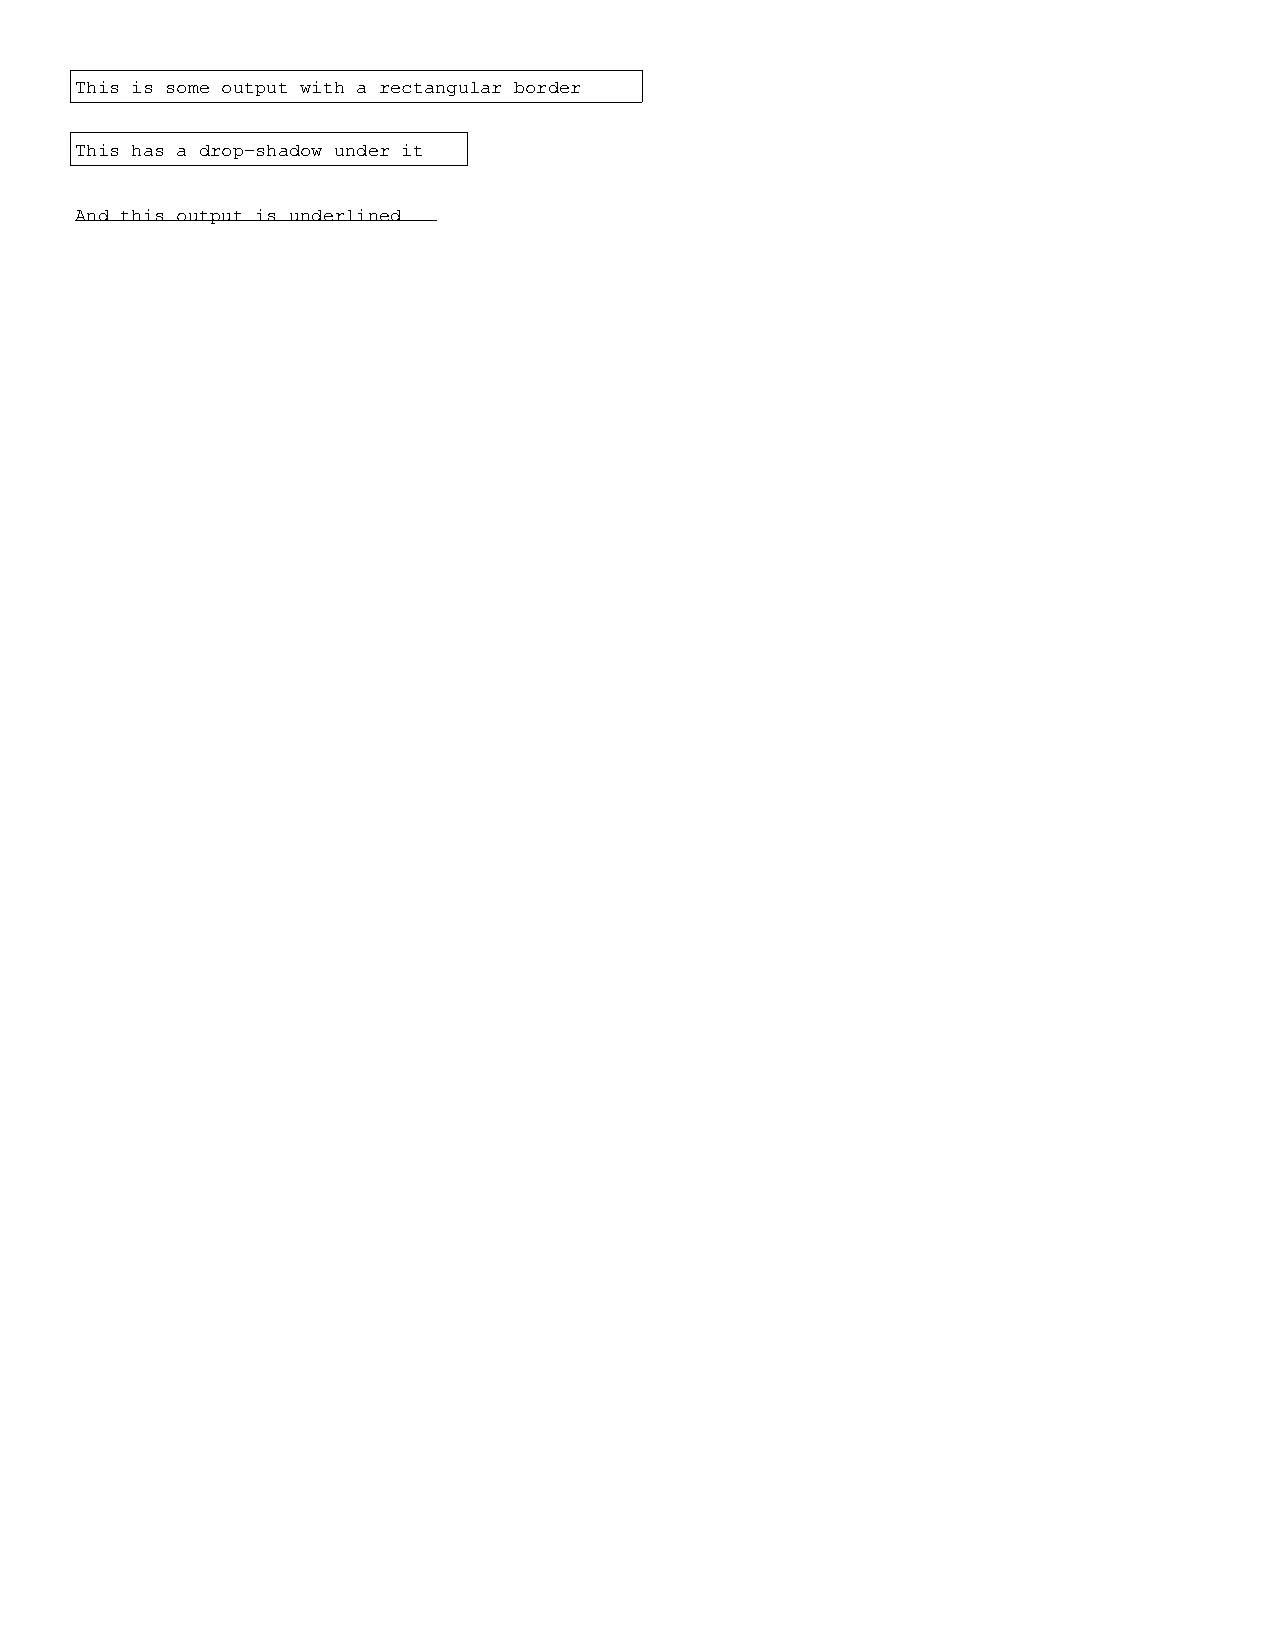
\includegraphics{border-example}}
\caption{\label{border-example} Examples of bordered output.}
\end{figure}


\Defmacro {surrounding-output-with-border} {(\optional stream
                                             \rest drawing-options
                                             \key shape (move-cursor \cl{t}))
                                            \body body}

Binds the local environment in such a way the output of \arg{body} will be
surrounded by a border of the specified shape.  Every implementation must
support the shapes \cl{:rectangle} (the default), \cl{:oval}, \cl{:drop-shadow},
and \cl{:underline}.  \cl{:rectangle} draws a rectangle around the bounding
rectangle of the output.  \cl{:oval} draws an oval around the bounding rectangle
of the output.  \cl{:drop-shadow} draws a ``drop shadow'' around the lower right
edge of the bounding rectangle of the output.  \cl{:underline} draws a thin line
along the baseline of all of the text in the output, but does not draw anything
underneath non-textual output.  \arg{drawing-options} is a list of drawing
options that are passed to the function that draws the border.

If the boolean \arg{move-cursor} is \term{true} (the default), then the text
cursor will be moved so that it immediately follows the lower right corner of
the bordered output.

\arg{stream} is an output recording stream to which output will be done.
The \arg{stream} argument is not evaluated, and must be a symbol that is
bound to a stream.  If \arg{stream} is \cl{t} (the default),
\cl{*standard-output*} is used.  \arg{body} may have zero or more
declarations as its first forms.

There are several strategies for implementing borders.  One strategy is to
create a ``border output record'' that contains the output records produced by
the output of \arg{body}, plus one or more output records that represent the
border.  Another strategy might be to arrange to call the border drawer at the
appropriate times without explicitly recording it.


\Defmacro {define-border-type} {shape arglist \body body}

Defines a new kind of border named \arg{shape}.  \arg{arglist} must be a subset
of the ``canonical'' arglist below (using \cl{string-equal} to do the
comparison):
\\
\arg{(\key stream record left top right bottom)}
\\

\arg{arglist} may include other keyword arguments that serve as the drawing options.

\arg{body} is the code that actually draws the border.  It has lexical access to
\cl{stream}, \cl{record}, \cl{left}, \cl{top}, \cl{right}, and \cl{bottom},
which are respectively, the stream being drawn on, the output record being
surrounded, and the coordinates of the left, top, right, and bottom edges of the
bounding rectangle of the record.  \arg{body} may have zero or more declarations
as its first forms.

% -*- Mode: LaTeX; Package: CLIM-USER -*-

\chapter {Text Formatting}
\label {text-formatting}

\section {Textual List Formatting}

\Defun {format-textual-list} {sequence printer
                              \key stream separator conjunction}

Outputs the sequence of items in \arg{sequence} as a ``textual list''.  For
example, the list \cl{(1 2 3 4)} might be printed as
\begin{verbatim}
1, 2, 3, and 4
\end{verbatim}

\arg{printer} is a function of two arguments: an element of the sequence and a
stream; it has dynamic extent.  It is called to output each element of the
sequence.

\arg{stream} specifies the output stream.  The default is \cl{*standard-output*}.

The \arg{separator} and \arg{conjunction} arguments provide control over the
appearance of each element of the sequence and over the separators used between
each pair of elements.  \arg{separator} is a string that is output after every
element but the last one; the default for \arg{separator} is \cl{", "} (that is,
a comma followed by a space).  \arg{conjunction} is a string that is output
before the last element.  The default is \cl{nil}, meaning that there is no
conjunction.  Typical values for \arg{conjunction} are the strings \cl{"and"}
and \cl{"or"}.


\section {Indented Output}

\Defmacro {indenting-output} {(stream indentation \key (move-cursor \cl{t}))
                              \body body}

Binds \arg{stream} to a stream that inserts whitespace at the beginning of each
line of output produced by \arg{body}, and then writes the indented output to
the stream that is the original value of \arg{stream}.

The \arg{stream} argument is not evaluated, and must be a symbol that is bound to
an output recording stream.  If \arg{stream} is \cl{t}, \cl{*standard-output*} is
used.  \arg{body} may have zero or more declarations as its first forms.

\arg{indentation} specifies how much whitespace should be inserted at the
beginning of each line.  It is specified in the same way as the \cl{:x-spacing}
option to \cl{formatting-table}.

If the boolean \arg{move-cursor} is \term{true} (the default), CLIM moves the
cursor to the end of the table.

Programmers using \cl{indenting-output} should begin the body with a call to
\arg{fresh-line} (or some equivalent) to position the stream to the initial
indentation.

{\bf Implementation note:} Some CLIM implementations restrict the use of
\cl{indenting-output} and \cl{filling-output} such that a call to
\cl{indenting-output} should appear outside of a call to \cl{filling-output}.
Implementations are encouraged to relax this restriction if the behavior is
well-defined, but uses of \cl{indenting-output} inside of \cl{filling-output}
may not be portable.


\section {Filled Output}

\Defmacro {filling-output} {(stream \key fill-width break-characters
                                         after-line-break after-line-break-initially) 
                            \body body}

Binds \arg{stream} to a stream that inserts line breaks into the textual output
written to it (by such functions as \cl{write-char} and \cl{write-string}) so
that the output is usually no wider then \arg{fill-width}.  The filled output is
then written on the original stream.

The \arg{stream} argument is not evaluated, and must be a symbol that is bound
to a stream.  If \arg{stream} is \cl{t}, \cl{*standard-output*} is used.
\arg{body} may have zero or more declarations as its first forms.

\arg{fill-width} specifies the width of filled lines, and defaults to 80
characters.  It is specified the same way as the \cl{:x-spacing} option for
\cl{formatting-table}.

``Words'' are separated by the characters specified in the list
\arg{break-characters}.  When a line is broken to prevent wrapping past the end
of a line, the line break is made at one of these separators.  That is,
\cl{filling-output} does not split ``words'' across lines, so it might produce
output wider than \arg{fill-width}.

\arg{after-line-break} specifies a string to be sent to \arg{stream} after line
breaks; the string appears at the beginning of each new line.  The string must
not be wider than \arg{fill-width}.

If the boolean \arg{after-line-break-initially} is \term{true}, then the
\arg{after-line-break} text is to be written to \arg{stream} before executing
\arg{body}, that is, at the beginning of the first line.  The default is
\term{false}.

% -*- Mode: LaTeX; Package: CLIM-USER -*-

\chapter {Incremental Redisplay}
\label {incremental-redisplay}

\section {Overview of Incremental Redisplay}

CLIM's incremental redisplay facility to allows the programmer to change the
output in an output history (and hence, on the screen or other output device) in
an incremental fashion.  It allows the programmer to redisplay individual pieces
of the existing output differently, under program control.  It is
``incremental'' in the sense that CLIM will try to minimize the changes to the
existing output on a display device when displaying new output.

There are two different ways to do incremental redisplay.

The first is to call \cl{redisplay} on an output record.  In essence, this tells
CLIM to recompute the output of that output record over from scratch.  CLIM
compares the new results with the existing output and tries to do minimal
redisplay.  The \cl{updating-output} form allows the programmer to assist CLIM
by informing it that entire branches of the output history are known not to have
changed.  \cl{updating-output} also allows the programmer to communicate the
fact that a piece of the output record hierarchy has moved, either by having an
output record change its parent, or by having an output record change its
position.

The second way to do incremental redisplay is for the programmer to manually do the
updates to the output history, and then call \cl{note-output-record-child-changed}
on an output record.  This causes CLIM to propagate the changes up the output
record tree and allows parent output records to re-adjust themselves to account for
the changes.

Each style is appropriate under different circumstances.  \cl{redisplay} is
often easier to use, especially when there might be large numbers of changes
between two passes, or when the programmer has only a poor idea as to what the
changes might be.  \cl{note-output-record-child-changed} can be more efficient
for small changes at the bottom of the output record hierarchy, or in cases
where the programmer is well informed as to the specific changes necessary and
can help CLIM out.


\subsection {Examples of Incremental Redisplay}

The usual technique of incremental redisplay is to use \cl{updating-output} to
inform CLIM what output has changed, and use \cl{redisplay} to recompute and
redisplay that output.

The outermost call to \cl{updating-output} identifies a program fragment that
produces incrementally redisplayable output.  A nested call to
\cl{updating-output} (that is, a call to \cl{updating-output} that occurs during
the execution of the body of the outermost \cl{updating-output} and specifies
the same stream) identifies an individually redisplayable piece of output, the
program fragment that produces that output, and the circumstances under which
that output needs to be redrawn.  This nested calls to \cl{updating-output} are
just hints to incremental redisplay that can reduce the amount of work done by
CLIM.

The outermost call to \cl{updating-output} executes its body, producing the
initial version of the output, and returns an \cl{updating-output-record} that
captures the body in a closure.  Each nested call to \cl{updating-output} stores
its \cl{:unique-id} and \cl{:cache-value} arguments and the portion of the
output produced by its body.

\cl{redisplay} takes an \cl{updating-output-record} and executes the captured
body of \cl{updating-output} over again.  When a nested call to
\cl{updating-output} is executed during redisplay, \cl{updating-output} decides
whether the cached output can be reused or the output needs to be redrawn.  This
is controlled by the \cl{:cache-value} argument to \cl{updating-output}.  If its
value matches its previous value, the body would produce output identical to the
previous output and thus it is unnecessary for CLIM to execute the body again.
In this case the cached output is reused and \cl{updating-output} does not
execute its body.  If the cache value does not match, the output needs to be
recomputed, so \cl{updating-output} executes its body and the new output drawn
on the stream replaces the previous output.  The \cl{:cache-value} argument is
only meaningful for nested calls to \cl{updating-output}.

In order to compare the cache to the output record, two pieces of information
are necessary:

\begin{itemize}
\item An association between the output being done by the program and a
particular cache.  This is supplied in the \cl{:unique-id} option to
\cl{updating-output}.

\item A means of determining whether this particular cache is valid.  This is
the \cl{:cache-value} option to \cl{updating-output}.
\end{itemize}

Normally, the programmer would supply both options. The unique-id would be some
data structure associated with the corresponding part of output.  The cache
value would be something in that data structure that changes whenever the output
changes.

It is valid to give the \cl{:unique-id} and not the \cl{:cache-value}.  This is
done to identify a parent in the hierarchy.  By this means, the children
essentially get a more complex unique id when they are matched for output.  (In
other words, it is like using a telephone area code.)  The cache without a cache
value is never valid.  Its children always have to be checked.

It is also valid to give the \cl{:cache-value} and not the \cl{:unique-id}.  In
this case, unique ids are just assigned sequentially.  So, if output associated
with the same thing is done in the same order each time, it isn't necessary to
invent new unique ids for each piece.  This is especially true in the case of
children of a cache with a unique id and no cache value of its own.  In this
case, the parent marks the particular data structure, whose components can
change individually, and the children are always in the same order and properly
identified by their parent and the order in which they are output.

A unique id need not be unique across the entire redisplay, only among the
children of a given output cache; that is, among all possible (current and
additional) uses made of \cl{updating-output} that are dynamically (not
lexically) within another.

To make incremental redisplay maximally efficient, the programmer should attempt
to give as many caches with \cl{:cache-value} as possible.  For instance, if the
thing being redisplayed is a deeply nested tree, it is better to be able to know
when whole branches have not changed than to have to recurse to every single
leaf and check it.  So, if there is a modification tick in the leaves, it is
better to also have one in their parent of the leaves and propagate the
modification up when things change.  While the simpler approach works, it
requires CLIM to do more work than is necessary.

The following function illustrates the standard use of incremental redisplay:

\begin{verbatim}
(defun test (stream)
  (let* ((list (list 1 2 3 4 5))
         (record
           (updating-output (stream)
             (do* ((elements list (cdr elements))
                   (count 0 (1+ count)))
                  ((null elements))
               (let ((element (first elements)))
                 (updating-output (stream :unique-id count
                                          :cache-value element)
                   (format stream "Element ~D" element)
                   (terpri stream)))))))
    (sleep 10)
    (setf (nth 2 list) 17)
    (redisplay record stream)))
\end{verbatim}

When this function is run on a window, the initial display will look like:

\begin{verbatim}
  Element 1
  Element 2
  Element 3
  Element 4
  Element 5
\end{verbatim}

After the sleep has terminated, the display will look like:

\begin{verbatim}
  Element 1
  Element 2
  Element 17
  Element 4
  Element 5
\end{verbatim}

CLIM takes care of ensuring that only the third line gets erased and
redisplayed.  In the case where items moved around (try the example substituting

\begin{verbatim}
(setq list (sort list #'(lambda (x y)
                          (declare (ignore x y))
                          (zerop (random 2))))) 
\end{verbatim}

for the form after the call to \cl{sleep}), CLIM would ensure that the minimum
amount of work would be done in updating the display, thereby minimizing
``flashiness'' while providing a powerful user interface.

See Chapter~\ref{application-frames} for a discussion of how to use incremental
redisplay automatically within the panes of an application frame.


\section {Standard Programmer Interface}

\Defmacro {updating-output} {(stream
                              \rest args
                              \key unique-id (id-test \#'\cl{eql})
                                   cache-value (cache-test \#'\cl{eql})
                                   fixed-position all-new parent-cache
                                   record-type)
                             \body body}

Introduces a caching point for incremental redisplay.  

The \arg{stream} argument is not evaluated, and must be a symbol that is bound to
an output recording stream.  If \arg{stream} is \cl{t}, \cl{*standard-output*} is
used.  \arg{body} may have zero or more declarations as its first forms.

\arg{record-type} specifies the class of output record to create.  The default
is \cl{standard-updating-output-record}.  This argument should only be supplied
by a programmer if there is a new class of output record that supports the
updating output record protocol.

\cl{updating-output} must be implemented by expanding into a call to
\cl{invoke-updating-output}, supplying a function that executes \arg{body} as
the \arg{continuation} argument to \cl{invoke-updating-output}.  The exact
behavior of this macro is described under \cl{invoke-updating-output}.

\Defgeneric {invoke-updating-output} {stream continuation record-type
                                      unique-id id-test
                                      cache-value cache-test
                                      \key all-new parent-cache}

Introduces a caching point for incremental redisplay.  Calls the function
\arg{continuation}, which generates the output records to be redisplayed.
\arg{continuation} is a function of one argument, the stream; it has dynamic
extent.

If this is used outside the dynamic scope of an incremental redisplay, it has no
particular effect.  However, when incremental redisplay is occurring, the
supplied \arg{cache-value} is compared with the value stored in the cache
identified by \arg{unique-id}.  If the values differ or the code in \arg{body}
has not been run before, the code in \arg{body} runs, and \arg{cache-value} is
saved for next time.  If the cache values are the same, the code in \arg{body}
is not run, because the current output is still valid.

\arg{unique-id} provides a means to uniquely identify the output done by
\arg{body}.  If \arg{unique-id} is not supplied, CLIM will generate one that is
guaranteed to be unique.  \arg{unique-id} may be any object as long as it is
unique with respect to the \arg{id-test} predicate among all such unique ids in
the current incremental redisplay.  \arg{id-test} is a function of two arguments
that is used for comparing unique ids; it has indefinite extent.

\arg{cache-value} is a value that remains constant if and only if the output
produced by body does not need to be recomputed.  If the cache value is not
supplied, CLIM will not use a cache for this piece of output.  \arg{cache-test}
is a function of two arguments that is used for comparing cache values; it has
indefinite extent.

If \arg{fixed-position} is \term{true}, then the location of this output is
fixed relative to its parent output record.  When CLIM redisplays an output
record that has a fixed position, then if the contents have not changed, the
position of the output record will not change.  If the contents have changed,
CLIM assumes that the code will take care to preserve its position.  The default
for \arg{fixed-position} is \term{false}.

If \arg{all-new} is \term{true}, that indicates that all of the output done by
\arg{body} is new, and will never match output previously recorded.  In this
case, CLIM will discard the old output and do the redisplay from scratch.  The
default for \arg{all-new} is \term{false}.

The output record tree created by \cl{updating-output} defines a caching
structure where mappings from a unique-id to an output record are maintained.
If the programmer specifies an output record $P$ via the
\arg{parent-cache} argument, then CLIM will try to find a corresponding output
record with the matching unique-id in the cache belonging to $P$.  If 
\arg{parent-cache} is not provided, then CLIM looks for the unique-id in the
output record created by immediate dynamically enclosing call to
\cl{updating-output}.  If that fails, CLIM uses the unique-id to find an output
record that is a child of the output history of \arg{stream}.  Once CLIM has
found an output record that matches the unique-id, it uses the cache value and
cache test to determine whether the output record has changed.  If the output
record has not changed, it may have moved, in which case CLIM will simply move
the display of the output record on the display device.


\Defun {redisplay} {record stream \key (check-overlapping \cl{t})}

This function simply calls \cl{redisplay-output-record} on the arguments
\arg{record} and \arg{stream}.

\Defgeneric {redisplay-output-record} {record stream
                                       \optional (check-overlapping \cl{t}) 
                                                 x y parent-x parent-y}  

\issue {SWM} {The coordinate system stuff affected by the x/y and parent-x/y
arguments is entirely bogus.  The proposal to make ``stream relative''
coordinates for output records instead of ``parent relative'' coordinates will
eliminate this completely.}

\cl{(redisplay-output-record \arg{record} \arg{stream})} causes the output of
\arg{record} to be recomputed.
CLIM redisplays the changes ``incrementally'', that is, it only displays those
parts that have been changed. \arg{record} must already be part of the output
history of the \term{output recording stream} \arg{stream}, although it can be
anywhere inside the hierarchy.

When \arg{check-overlapping} is \term{false}, this means that CLIM can assume
that no sibling output records overlap each other at any level in the output
record tree.  Supplying a \term{false} value for this argument can improve
performance of redisplay.

{\bf Implementation note:} \cl{redisplay-output-record} is implemented by first
binding \cl{stream-redisplaying-p} of the stream to \term{true}, then creating
the new output records by invoking \cl{compute-new-output-records}.  Once the
new output records have been computed, \cl{compute-difference-set} is called to
compute the difference set, which is then passed to
\cl{note-child-output-record-changed}.

The other optional arguments can be used to specify where on the \arg{stream}
the output record should be redisplayed.  \arg{x} and \arg{y} represent where
the cursor should be, relative to (\cl{output-record-parent} record), before we
start redisplaying \arg{record}.  \arg{parent-x} and \arg{parent-y} can be
supplied to say: do the output as if the parent started at positions
\arg{parent-x} and \arg{parent-y} (which are in absolute coordinates).  The
default values for \arg{x} and \arg{y} are \cl{(output-record-start-position
\arg{record})}.  The default values for \arg{parent-x} and \arg{parent-y} are

\begin{verbatim}
(convert-from-relative-to-absolute-coordinates 
    stream
    (output-record-parent record))
\end{verbatim}

\arg{record} will usually be an output record created by \cl{updating-output}.
If it is not, then \cl{redisplay-output-record} will be equivalent to
\cl{replay-output-record}.


\section {Incremental Redisplay Protocol}

\Issue {SWM} {While the description of the API here is accurate, the description
of the protocol is a disaster.  This is no surprise, since the protocol for
increment redisplay is itself a disaster.}

\Defprotoclass {updating-output-record}

The protocol class corresponding to records that support incremental redisplay;
a subclass of \cl{output-record}.
\IfYouWantClass {an} {updating output record} {updating-output-record}

\Defpredicate {updating-output-record-p} {object}

Returns \term{true} if \arg{object} is an \term{updating output record},
otherwise returns \term{false}.

\definitarg {:unique-id}
\definitarg {:id-test}
\definitarg {:cache-value}
\definitarg {:cache-test}
\Definitarg {:fixed-position}

All subclasses of \cl{updating-output-record} must handle these four initargs,
which are used to specify, respectively, the unique id and id test, cache value
and cache test, and the ``fixed position'' component of the output record.

\Defclass {standard-updating-output-record}

The instantiable class of output record that supports incremental redisplay.
This is a subclass of \cl{updating-output-record}.


\Defgeneric {output-record-unique-id} {record}

Returns the unique id associated with the updating output record \arg{record}.

\Defgeneric {output-record-cache-value} {record}

Returns the cache value associated with the updating output record \arg{record}.

\Defgeneric {output-record-fixed-position} {record}

Returns \term{true} if the updating output record \arg{record} is at a fixed
location on the output stream, otherwise returns \term{false}.  Output records
that are not at fixed location on the output stream will be moved by incremental
redisplay when any of their siblings adjust their size or position.

\Defgeneric {output-record-displayer} {record}

Returns the function that produces the output for this output record.  This is
the function that is called during redisplay to produce new output if the cache
value mismatches.


\Defgeneric {compute-new-output-records} {record stream}

\cl{compute-new-output-records} modifies an output record tree to reflect new
output done by the application.  In addition to inserting the new output records
into the output record tree, it must save enough information to be able to
compute the difference set, such as the old bounding rectangle, old cursor
positions, old children, and so forth.

\cl{compute-new-output-records} recursively invokes itself on each child of
\arg{record}.

\cl{compute-new-output-records} of an output record of type
\cl{updating-output-record} runs the displayer (\cl{output-record-displayer}),
which gives the behavior of incremental redisplay.  That is, it reruns the code
(getting hints from \cl{updating-output}) and figures out the changes from there
by comparing it to the old output history.


\Defgeneric {compute-difference-set} {record \optional (check-overlapping \cl{t})
                                      (offset-x \cl{0}) (offset-y \cl{0})
                                      (old-offset-x \cl{0}) (old-offset-y \cl{0})} 

\cl{compute-difference-set} compares the current state of the \term{output
record} \arg{record} with its previous state, and returns a ``difference set''
as five values.  The difference set controls what needs to be done to the
display device in order to accomplish the incremental redisplay.

The values returned are \arg{erases} (what areas of the display device need to
be erased), \arg{moves} (what output records need to be moved), \arg{draws}
(what output records need to be freshly replayed), \arg{erase-overlapping}, and
\arg{move-overlapping}.  Each is a list whose elements are lists of the form:

\begin{itemize}
\item \arg{erases} are lists of \cl{(\arg{record} \arg{old-box})}

\item \arg{moves} are lists of \cl{(\arg{record} \arg{old-box} \arg{new-position})}

\item \arg{draws} are lists of \cl{(\arg{record} \arg{old-box})}

\item \arg{erase-overlapping} is a list of \cl{(\arg{record} \arg{old-box})}

\item \arg{move-overlapping} is a list of \cl{(\arg{record} \arg{old-box} \arg{new-position})}
\end{itemize}

When \arg{check-overlapping} is \term{false}, this means that CLIM can assume
that no sibling output records overlap each other at any level.  Supplying a
\term{false} value for this argument can improve performance of redisplay.


\Defgeneric {augment-draw-set} {record erases moves draws erase-overlapping move-overlapping
                                \optional x-offset y-offset old-x-offset old-y-offset}

\issue {SWM} {To be supplied.}


\Defgeneric {note-output-record-child-changed}
            {record child mode old-position old-bounding-rectangle stream
             \optional erases moves draws erase-overlapping move-overlapping
             \key check-overlapping}

\cl{note-output-record-child-changed} is called after an output history has had
changes made to it, but before any of the new output has been displayed.  It
will call \cl{propagate-output-record-changes-p} to determine if the parent
output record should be notified, and if so, will call
\cl{propagate-output-record-changes} to create an updated difference set.  If no
changes need to be propagated to the parent output record, then
\cl{note-output-record-child-changed} will call \cl{incremental-redisplay} in
order to display the difference set.

\arg{mode} is one of \cl{:delete}, \cl{:add}, \cl{:change}, \cl{:move}, or
\cl{:none}.

\arg{old-position} and \arg{old-bounding-rectangle} describe where \arg{child}
was before it was moved.

\arg{check-overlapping} is as for \cl{compute-difference-set}.


\Defgeneric {propagate-output-record-changes-p} {record child mode 
                                                 old-position old-bounding-rectangle}

\cl{propagate-output-record-changes-p} is a predicate that returns \term{true}
if the change made to the child will cause \arg{record} to be redisplayed in any
way.  Otherwise, it returns \term{false}.  \arg{mode} is one of \cl{:delete},
\cl{:add}, \cl{:change}, \cl{:move}, or \cl{:none}.

\Defgeneric {propagate-output-record-changes} 
            {record child mode 
             \optional old-position old-bounding-rectangle
                       erases moves draws erase-overlapping move-overlapping check-overlapping}

Called when the changed \arg{child} output record requires that its parent,
\arg{record}, be redisplayed as well.  \cl{propagate-output-record-changes}
will update the difference set to reflect the additional changes.

\arg{check-overlapping} is as for \cl{compute-difference-set}.


\Defgeneric {match-output-records} {record \rest initargs}

Returns \term{true} if record matches the supplied class initargs
\arg{initargs}, otherwise returns \term{false}.

\Defgeneric {find-child-output-record} {record use-old-elements record-type
                                        \rest initargs
                                        \key unique-id unique-id-test}

Finds a child of \arg{record} matching the \arg{record-type} and the supplied
initargs \arg{initargs}.  \arg{unique-id} and \arg{unique-id-test} are used to
match against the children as well.  \arg{use-old-elements} controls whether the
desired record is to be found in the previous (before redisplay) contents of the
record.

\Defgeneric {output-record-contents-ok} {record}

Returns \term{true} if the current state of \arg{record} are up to date,
otherwise returns \term{false}.

\Defgeneric {recompute-contents-ok} {record}

Compares the old (before redisplay) and new contents of \arg{record} to
determine whether or not this record changed in such a way so that the display
needs updating.

\Defgeneric {cache-output-record} {record child unique-id}

\arg{record} stores \arg{child} such that it can be located later using
\arg{unique-id}.

\Defgeneric {decache-child-output-record} {record child use-old-elements}

Invalidates the redisplay state of \arg{record}.

\Defgeneric {find-cached-output-record} {record use-old-elements record-type
                                         \rest initargs
                                         \key unique-id unique-id-test \allow}

Finds a previously cached child matching \arg{record-type}, \arg{initargs},
\arg{unique-id}, and \arg{unique-id-test}.  \arg{use-old-elements} controls
whether the desired record is to be found in the previous (before redisplay)
contents of the record.


\section {Incremental Redisplay Stream Protocol}

\Defgeneric {redisplayable-stream-p} {stream}

Returns \term{true} for any stream that maintains an output history and supports
the incremental redisplay protocol, otherwise returns \term{false}.

\Defgeneric {stream-redisplaying-p} {stream}

Returns \term{true} if the \arg{stream} is currently doing redisplay (that is,
is inside of a call to \cl{redisplay}), otherwise returns \term{false}.

\Defgeneric {incremental-redisplay} {stream position
                                     erases moves draws erase-overlapping move-overlapping} 

Performs the incremental update on \arg{stream} according to the difference set
comprised by \arg{erases}, \arg{moves}, \arg{draws}, \arg{erase-overlapping},
and \arg{move-overlapping}, which are values returned by
\cl{compute-difference-set}.  \arg{position} is a point object that represents
the start position of the topmost output record that will be redisplayed.

\cl{incremental-redisplay} can be called on any extended output stream.


\part{Extended Stream Input Facilities}
% -*- Mode: LaTeX; Package: CLIM-USER -*-

\chapter {Extended Stream Input}
\label {extended-input}

CLIM provides a stream-oriented input layer that is implemented on top of the
sheet input architecture.  The basic CLIM input stream protocol is based on the
character input stream protocol proposal submitted to the ANSI Common Lisp
committee by David Gray.  This proposal was not approved by the committee, but
has been implemented by most Lisp vendors.

\section {Basic Input Streams}

CLIM provides an implementation of the basic input stream facilities (described
in more detail in Appendix~\ref{gray-streams}), either by directly using the
underlying Lisp implementation, or by implementing the facilities itself.

\Defclass {standard-input-stream}

This class provides an implementation of the CLIM's basic input stream protocol
based on CLIM's input kernel.  It defines a \cl{handle-event} method for
keystroke events and queues the resulting characters in a per-stream input
buffer.
\Mutable

\Defgeneric {stream-read-char} {stream}

Returns the next character available in the \term{input stream} \arg{stream}, or
\cl{:eof} if the stream is at end-of-file.  If no character is available this
function will wait until one becomes available.

\Defgeneric {stream-read-char-no-hang} {stream}

Like \cl{stream-read-char}, except that if no character is available the
function returns \term{false}.

\Defgeneric {stream-unread-char} {stream character}

Places the character \arg{character} back into the \term{input stream}
\arg{stream}'s input buffer.  The next call to \cl{read-char} on \arg{stream}
will return the unread character.  The character supplied must be the most
recent character read from the stream.

\Defgeneric {stream-peek-char} {stream}

Returns the next character available in the \term{input stream} \arg{stream}.
The character is not removed from the input buffer.  Thus, the same character
will be returned by a subsequent call to \cl{stream-read-char}.

\Defgeneric {stream-listen} {stream}

Returns \term{true} if there is input available on the \term{input stream}
\arg{stream}, \term{false} if not.

\Defgeneric {stream-read-line} {stream}

Reads and returns a string containing a line of text from the \term{input
stream} \arg{stream}, delimited by the \verb+#\Newline+ character.

\Defgeneric {stream-clear-input} {stream}

Clears any buffered input associated with the \term{input stream} \arg{stream},
and returns \term{false}.


\section {Extended Input Streams}

In addition to the basic input stream protocol, CLIM defines an extended input
stream protocol.  This protocol extends the stream model to allow manipulation
of non-character user gestures, such as pointer button presses.  The extended
input protocol provides the programmer with more control over input processing,
including the options of specifying input wait timeouts and auxiliary input test
functions.

\Defprotoclass {extended-input-stream}

The protocol class for CLIM extended input streams.  This is a subclass of
\cl{input-stream}.
\IfYouWantClass {an} {extended input stream} {extended-input-stream}

\Defpredicate {extended-input-stream-p} {object}

Returns \term{true} if \arg{object} is a CLIM \term{extended input stream},
otherwise returns \term{false}.

\definitarg {:input-buffer}
\definitarg {:pointer}
\Definitarg {:text-cursor}

All subclasses of \cl{extended-input-stream} must handle these initargs, which
are used to specify, respectively, the input buffer, pointer, and text cursor
for the extended input stream.

\Defclass {standard-extended-input-stream}

This class provides an implementation of the CLIM extended input stream protocol
based on CLIM's input kernel.  The extended input stream maintains the state of
the display's pointing devices (such as a mouse) in pointer objects associated
with the stream.  It defines a \cl{handle-event} methods for keystroke and
pointer motion and button press events and updates the pointer object state and
queues the resulting events in a per-stream input buffer.

\Mutable


\subsection {The Extended Input Stream Protocol}

The following generic functions comprise the extended input stream protocol.
All extended input streams must implement methods for these generic functions.

\Defgeneric {stream-input-buffer} {stream}
\Defgeneric {(setf stream-input-buffer)} {buffer stream}

The functions provide access to the stream's input buffer.  Normally programs do
not need to manipulate the input buffer directly.  It is sometimes useful to
cause several streams to share the same input buffer so that input that comes in
on one of them is available to an input call on any of the streams.  The input
buffer must be vector with a fill pointer capable of holding general input
gesture objects (such as characters and event objects).

\Defgeneric {stream-pointer-position} {stream \key pointer}

Returns the current position of the pointing device \arg{pointer} for the
\term{extended input stream} \arg{stream} as two values, the $x$ and $y$
positions in the stream's drawing surface coordinate system.  If \arg{pointer}
is not supplied, it defaults to \cl{port-pointer} of the stream's port.

\Defgeneric {(setf* stream-pointer-position)} {x y stream \key pointer}

Sets the position of the pointing device for the \term{extended input stream}
\arg{stream} to \arg{x} and \arg{y}, which are integers.  \arg{pointer} is as
for \cl{stream-pointer-position}.

For CLIM implementations that do not support \cl{setf*}, the ``setter'' function
for this is \cl{stream-set-pointer-position}.

\Defgeneric {stream-set-input-focus} {stream}

Sets the ``input focus'' to the \term{extended input stream} \arg{stream} by
changing the value of \cl{port-keyboard-input-focus} and returns the old input
focus as its value.

\Defmacro {with-input-focus} {(stream) \body body}

Temporarily gives the keyboard input focus to the \term{extended input stream}
\arg{stream}.  By default, an application frame gives the input focus to the
window associated with \cl{frame-query-io}.

The \arg{stream} argument is not evaluated, and must be a symbol that is bound
to a stream.  If \arg{stream} is \cl{t}, \cl{*standard-input*} is used.
\arg{body} may have zero or more declarations as its first forms.


\defvar {*input-wait-test*}
\defvar {*input-wait-handler*}
\Defvar {*pointer-button-press-handler*}

These three variables are used to hold the default values for the current input
wait test, wait handler, and pointer button press handler.  These variables are
globally bound to \cl{nil}.


\Defun {read-gesture} {\key (stream \cl{*standard-input*})
                            timeout peek-p 
                            (input-wait-test \cl{*input-wait-test*})
                            (input-wait-handler \cl{*input-wait-handler*})
                            (pointer-button-press-handler \cl{*pointer-button-press-handler*})}

Calls \cl{stream-read-gesture} on the \term{extended input stream} \arg{stream}
and all of the other keyword arguments.  These arguments are the same as for
\cl{stream-read-gesture}.

\Defgeneric {stream-read-gesture} {stream
                                   \key timeout peek-p 
                                        (input-wait-test \cl{*input-wait-test*})
                                        (input-wait-handler \cl{*input-wait-handler*})
                                        (pointer-button-press-handler \cl{*pointer-button-press-handler*})}

Returns the next gesture available in the \term{extended input stream}
\arg{stream}; the gesture will be either a character or an event (such as a
pointer button event).  The input is not echoed.

If the user types an abort gesture (that is, a gesture that matches any of the
gesture names in \cl{*abort-gestures*}), then the \cl{abort-gesture} condition
will be signalled.

If the user types an accelerator gesture (that is, a gesture that matches any of
the gesture names in \cl{*accelerator-gestures*}), then the \cl{accelerator-gesture}
condition will be signalled.

\cl{stream-read-gesture} works by invoking \cl{stream-input-wait} on
\arg{stream}, \arg{input-wait-test}, and \arg{timeout}, and then processing the
input, if there is any.  \cl{:around} methods on this generic function can be
used to implement some sort of a gesture preprocessing mechanism on every
gesture; CLIM's input editor will typically be implemented this way.

\arg{timeout} is either \cl{nil} or an integer that specifies the number of
seconds that \cl{stream-read-gesture} will wait for input to become available.
If no input is available, \cl{stream-read-gesture} will return two values,
\cl{nil} and \cl{:timeout}.

If the boolean \arg{peek-p} is \term{true}, then the returned gesture will be
left in the stream's input buffer.

\arg{input-wait-test} is a function of one argument, the stream.  The function
should return \term{true} when there is input to process, otherwise it should
return \term{false}.  This argument will be passed on to \cl{stream-input-wait}.
\cl{stream-read-gesture} will bind \cl{*input-wait-test*} to \arg{input-wait-test}.

\arg{input-wait-handler} is a function of one argument, the stream.  It is
called when \cl{stream-input-wait} returns \term{false} (that is, no input is
available).  This option can be used in conjunction with \arg{input-wait-test}
to handle conditions other than keyboard gestures, or to provide some sort of
interactive behavior (such as highlighting applicable presentations).
\cl{stream-read-gesture} will bind \cl{*input-wait-handler*} to
\arg{input-wait-handler}.

\arg{pointer-button-press-handler} is a function of two arguments, the stream
and a pointer button press event.  It is called when the user clicks a pointer
button.  \cl{stream-read-gesture} will bind \cl{*pointer-button-press-handler*}
to \arg{pointer-button-press-handler}.


\arg{input-wait-test}, \arg{input-wait-handler}, and
\arg{pointer-button-press-handler} have dynamic extent.


\Defgeneric {stream-input-wait} {stream \key timeout input-wait-test}

Waits for input to become available on the \term{extended input stream}
\arg{stream}.  \arg{timeout} and \arg{input-wait-test} are as for
\cl{stream-read-gesture}.


\Defun {unread-gesture} {gesture \key (stream \cl{*standard-input*})}

Calls \cl{stream-unread-gesture} on \arg{gesture} and \arg{stream}.  These
arguments are the same as for \cl{stream-unread-gesture}.

\Defgeneric {stream-unread-gesture} {stream gesture}

Places \arg{gesture} back into the \term{extended input stream} \arg{stream}'s
input buffer.  The next call to \cl{stream-read-gesture} request will return the
unread gesture.  The gesture supplied must be the most recent gesture read from
the stream via \cl{read-gesture}.


\subsection {Extended Input Stream Conditions}

\Defvar {*abort-gestures*}

A list of all of the gesture names that correspond to abort gestures.  The
exact global set of standard abort gestures is unspecified, but must include
the \cl{:abort} gesture name.

\Defcondition {abort-gesture}

This condition is signalled by \cl{read-gesture} whenever an abort gesture (one
of the gestures in \cl{*abort-gestures*} is read from the user.  This condition
will handle the \cl{:event} initarg, which is used to supply the event
corresponding to the abort gesture.

\Defgeneric {abort-gesture-event} {condition}

Returns the event that cause the abort gesture condition to be signalled.
\cl{condition} is an object of type \cl{abort-gesture}.

\Defvar {*accelerator-gestures*}

A list of all of the gesture names that correspond to keystroke accelerators.
The global value for this is \cl{nil}.

\Defcondition {accelerator-gesture}

This condition is signalled by \cl{read-gesture} whenever an keystroke
accelerator gesture (one of the gestures in \cl{*accelerator-gestures*} is read
from the user.  This condition will handle the \cl{:event} and the
\cl{:numeric-argument} initargs, which are used to supply the event
corresponding to the abort gesture and the accumulated numeric argument (which
defaults to 1).

\Defgeneric {accelerator-gesture-event} {condition}

Returns the event that caused the accelerator gesture condition to be signalled.
\cl{condition} is an object of type \cl{accelerator-gesture}.

\Defgeneric {accelerator-gesture-numeric-argument} {condition}

Returns the accumulated numeric argument (maintained by the input editor) at the
time the accelerator gesture condition was signalled.  \cl{condition} is an
object of type \cl{accelerator-gesture}.


\section {Gestures and Gesture Names\label{gesture-names}}

A \concept{gesture} is some sort of input action by the user, such as typing a
character or clicking a pointer button.  A \concept{keyboard gesture} refers to
those gestures that are input by typing something on the keyboard.  A
\concept{pointer gesture} refers to those gestures that are input by doing
something with the pointer, such as clicking a button.

A \concept{gesture name} is a symbol that gives a name to a set of similar
gestures.  Gesture names are used in order to provide a level of abstraction
above raw device events; greater portability can thus be achieved by avoiding
referring directly to platform-dependent constructs, such as character objects
that refer to a particular key on the keyboard.  For example, the \cl{:complete}
gesture is used to name the gesture that causes the \cl{complete-input} complete
the current input string; on Genera, this may correspond to the Complete key on
the keyboard (which generates a \verb+#\Complete+ character), but on a Unix
workstation, it may correspond to some other key.  Another example is
\cl{:select}, which is commonly used to indicate a left button click on the
pointer.

Note that gesture names participate in a one-to-many mapping, that is, a single
gesture name can name a group of physical gestures.  For example, an \cl{:edit}
might include both a pointer button click and a key press.

CLIM uses \term{event} objects to represent user gestures.  Some of the more
common events are those of the class \cl{pointer-button-event}.  Event objects
store the sheet associated with the event, a timestamp, and the modifier key
state (a quantity that indicates which modifier keys were held down on the
keyboard at the time the event occurred).  Pointer button event objects also
store the pointer object, the button that was clicked on the pointer, the window
the pointer was over and the $x$ and $y$ position within that window.  Keyboard
gestures store the key name.

In some contexts, the object used to represent a user gesture is referred to as
an \concept{gesture object}.  An gesture object might be exactly the same as an
event object, or might contain less information.  For example, for a keyboard
gesture that corresponds to a standard printing character, it may be enough to
represent the gesture object as a character.


\Defmacro {define-gesture-name} {name type gesture-spec \key (unique \cl{t})} 

Defines a new gesture named by the symbol \arg{name}.  \arg{type} is the type of
gesture being created, and must be one of the symbols described below.
\arg{gesture-spec} specifies the physical gesture that corresponds to the named
gesture; its syntax depends on the value of \arg{type}.
\cl{define-gesture-name} must expand into a call to \cl{add-gesture-name}.

If \arg{unique} is \term{true}, all old gestures named by \arg{name} are first
removed.  \arg{unique} defaults to \cl{t}.

None of the arguments to \cl{define-gesture-name} are evaluated.

\Defun {add-gesture-name} {name type gesture-spec \key unique}

Adds a gesture named by the symbol \arg{name} to the set of gesture names.
\arg{type} is the type of gesture being created, and must be one of the symbols
described below.  \arg{gesture-spec} specifies the physical gesture that
corresponds to the named gesture; its syntax depends on the value of \arg{type}.

If \arg{unique} is \term{true}, all old gestures named by \arg{name} are first
removed.  \arg{unique} defaults to \cl{nil}.

When \arg{type} is \cl{:keyboard}, \arg{gesture-spec} is a list of the form
\arg{(key-name . modifier-key-names)}.  \arg{key-name} is the name of a
non-modifier key on the keyboard (see below).  \arg{modifier-key-names} is a
(possibly empty) list of modifier key names (\cl{:shift}, \cl{:control},
\cl{:meta}, \cl{:super}, and \cl{:hyper}).

For the standard Common Lisp characters (the 95 ASCII printing characters
including \verb+#\Space+), \arg{key-name} is the character object itself.  For
the other ``semi-standard'' characters, \arg{key-name} is a keyword symbol
naming the character (\cl{:newline}, \cl{:linefeed}, \cl{:return}, \cl{:tab},
\cl{:backspace}, \cl{:page}, and \cl{:rubout}).  CLIM implementations may extend
the set of key names on a per-port basic, but should choose a port-specific
package.  For example, the Genera port might such gestures as include
\cl{genera-clim:help} and \cl{genera-clim:complete}.

The names of the modifier keys have been chosen to be uniform across all
platforms, even though not all platforms will have keys on the keyboard with
these names.  The per-port part of a CLIM implementation must simply choose a
sensible mapping from the modifier key names to the names of the keys on the
keyboard.  For example, a CLIM implementation on the Macintosh might map
\cl{:meta} to the Command shift key, and \cl{:super} to the Option shift key.

When \arg{type} is \cl{:pointer-button}, \cl{:pointer-button-press}, or
\cl{:pointer-button-release}, \arg{gesture-spec} is a list of the form
\arg{(button-name . modifier-key-names)}.  \arg{button} is the name of a pointer
button (\cl{:left}, \cl{:middle}, or \cl{:right}), and \arg{modifier-key-names}
is as above.

CLIM implementations are permitted to have other values of \arg{type} as an
extension, such as \cl{:pointer-motion} or \cl{:timer}.

As an example, the \cl{:edit} gesture name above could be defined as follows
using \cl{define-gesture-name}:

\begin{verbatim}
(define-gesture-name :edit :pointer-button (:left :meta))
(define-gesture-name :edit :keyboard (#\E :control))
\end{verbatim}

\Defun {delete-gesture-name} {name}

Removes the gesture named by the symbol \arg{name}.


\Defun {event-matches-gesture-name-p} {event gesture-name}

Returns \term{true} if the device event \arg{event} ``matches'' the gesture
named by \arg{gesture-name}.

For pointer button events, the event matches the gesture name when the pointer
button from the event matches the name of the pointer button one of the gesture
specifications named by \arg{gesture-name}, and the modifier key state from the
event matches the names of the modifier keys in that same gesture specification.

For keyboard events, the event matches the gesture name when the key name from
the event matches the key name of one of the gesture specifications named by
\arg{gesture-name}, and the modifier key state from the event matches the names
of the modifier keys in that same gesture specification.

\Defun {modifier-state-matches-gesture-name-p} {modifier-state gesture-name}

Returns \term{true} if the modifier key state from the device event \arg{event}
matches the names of the modifier keys in one of the gesture specifications
named by \arg{gesture-name}.

\issue {SWM} {Note that none of the functions above take a port argument.  This
is because CLIM implicitly assumes that the canonical set of gesture names is
the same on every port, and only the mappings differ from port to port.  Some
ports may define additional gesture names, but they will simply not be mapped on
other ports.  Is this a reasonable assumption?}

\Defun {make-modifier-state} {\rest modifiers}

Given a list of modifier state names, this creates an integer that serves as a
modifier key state.  The legal modifier state names are \cl{:shift},
\cl{:control}, \cl{:meta}, \cl{:super}, and \cl{:hyper}.


\subsection {Standard Gesture Names}

Every CLIM implementation must provide a standard set of gesture names that
correspond to a common set of gestures.  These gesture names must have a
meaningful mapping for every port type.

Here are the required, standard keyboard gesture names:

\begin{itemize}
\item \cl{:abort}---corresponds to gestures that cause the currently running
application to be aborted back to top-level.  On Genera, this will match the
\verb+#\Abort+ character.  On other systems, this may match the event
corresponding to typing {\tt Control-C}.

\item \cl{:clear-input}---corresponds to gestures that cause the current input
buffer to be cleared.  On Genera, this will match the \verb+#\Clear-Input+
character.  On other systems, this may match the event corresponding to typing
{\tt Control-U}.

\item \cl{:complete}---corresponds to the gestures that tell the completion
facility to complete the current input.  On most systems, this will typically
match the \verb+#\Tab+ or \verb+#\Escape+ character.  On Genera, this will match
the \verb+#\Complete+ character as well.

\item \cl{:help}---corresponds to the gestures that tell \cl{accept} and the
completion facility to display a help message.  On most systems, this will
typically match the event corresponding to typing {\tt Control-/}.  On Genera,
this will match the \verb+#\Help+ character as well.

\item \cl{:possibilities}---corresponds to the gestures that tell the completion
facility to display the current set of possible completions.  On most systems,
this will typically match the event corresponding to typing {\tt Control-?}.
\end{itemize}

Here are the required, standard pointer gesture names:

\begin{itemize}
\item{\cl{:select}}---corresponds to the gesture that is used to ``select'' the
object being pointed to with the pointer.  Typically, this will correspond to
the left button on the pointer.

\item{\cl{:describe}}---corresponds to the gesture that is used to ``describe''
or display some sort of documentation on the object being pointed to with the
pointer.  Typically, this will correspond to the middle button on the pointer.

\item{\cl{:menu}}---corresponds to the gesture that is used to display a menu of
all possible operation on the object being pointed to with the pointer.
Typically, this will correspond to the right button on the pointer.

\item{\cl{:edit}}---corresponds to the gesture that is used to ``edit'' the
object being pointed to with the pointer.  Typically, this will correspond to
the left button on the pointer with some modifier key held down (such as the
\cl{:meta} key).

\item{\cl{:delete}}---corresponds to the gesture that is used to ``delete'' the
object being pointed to with the pointer.  Typically, this will correspond to
the middle button on the pointer with some modifier key held down (such as the
\cl{:shift} key).
\end{itemize}


\section {The Pointer Protocol}

\Defprotoclass {pointer}

The protocol class that corresponds to a pointing device.
\IfYouWantClass {a} {pointer} {pointer}
\Mutable

\Defpredicate {pointerp} {object}

Returns \term{true} if \arg{object} is a \term{pointer}, otherwise returns
\term{false}.

\Definitarg {:port}

The \cl{:port} initarg is used to specify the port with which the pointer is
associated.

\Defclass {standard-pointer}

The instantiable class that implements a pointer.

\defgeneric {pointer-sheet} {pointer}
\Defgeneric {(setf pointer-sheet)} {sheet pointer}

Returns (or sets) the sheet over which the \term{pointer} \arg{pointer} is located.

\Defgeneric {pointer-button-state} {pointer}

Returns the current state of the buttons of the \term{pointer} \arg{pointer} as
an integer.  This will be a mask consisting of the \cl{logior} of
\cl{+pointer-left-button+}, \cl{+pointer-middle-button+}, and
\cl{+pointer-right-button+}.

\Defgeneric {pointer-position} {pointer}

Returns the $x$ and $y$ position of the \term{pointer} \arg{pointer} as two
values.

\Defgeneric {(setf* pointer-position)} {x y pointer}

Sets the $x$ and $y$ position of the \term{pointer} \arg{pointer} to the
specified position.

For CLIM implementations that do not support \cl{setf*}, the ``setter'' function
for this is \cl{pointer-set-position}.

\defgeneric {pointer-cursor} {pointer}
\Defgeneric {(setf pointer-cursor)} {cursor pointer}

A pointer object usually has a visible cursor associated with it.  These
functions return (or set) the cursor associated with the \term{pointer}
\arg{pointer}.

\Defmethod {port} {(pointer \cl{standard-pointer})}

Returns the port with which \arg{pointer} is associated.


\section {Pointer Tracking}

\Defmacro {tracking-pointer} {(sheet \key pointer multiple-window
                                          transformp context-type highlight)
                              \body body}

The \cl{tracking-pointer} macro provides a general means for running code while
following the position of a pointing device, and monitoring for other input
events.  The programmer supplies code (the clauses in \arg{body}) to be run upon
the occurrence of any of the following types of events:

\begin{itemize}
\item Motion of the pointer

\item Motion of the pointer over a presentation

\item Clicking or releasing a pointer button

\item Clicking or releasing a pointer button while the pointer is over a presentation

\item Keyboard event (typing a character)
\end{itemize}

The \arg{sheet} argument is not evaluated, and must be a symbol that is bound to
an input sheet or stream.  If \arg{sheet} is \cl{t}, \cl{*standard-output*} is
used.  \arg{body} may have zero or more declarations as its first forms.

The \arg{pointer} argument specifies a pointer to track.  It defaults to
the primary pointer for the sheet, \cl{(port-pointer (port \arg{sheet}))}.

When the boolean \arg{multiple-windows} is \term{true}, then the pointer will be
tracked across multiple windows, otherwise is will be tracked only in the window
corresponding to \arg{sheet}.

When the boolean \arg{transformp} is \term{true}, then the coordinates supplied
to the \cl{:pointer-motion} clause will be in the ``user'' coordinate system
rather than in stream coordinates, that is, the medium's transformation will be
applied to the coordinates.

\arg{context-type} is used to specify the presentation type of presentations
that will be ``visible'' to the tracking code for purposes of highlighting and
for the \cl{:presentation}, \cl{:presentation-button-press}, and
\cl{:presentation-button-release} clauses.  Supplying \arg{context-type} is only
useful when \arg{sheet} is an output recording stream.  \arg{context-type}
defaults to \cl{t}, meaning that all presentations are visible.

When \arg{highlight} is \term{true}, \cl{tracking-pointer} will highlight
applicable presentations as the pointer is positioned over them.  {highlight}
defaults to \term{true} when any of the \cl{:presentation},
\cl{:presentation-button-press}, or \cl{:presentation-button-release} clauses is
supplied, otherwise it defaults to \term{false}.  See
Chapter~\ref{output-recording} for a complete discussion of presentations.

The body of \cl{tracking-pointer} consists of a list of clauses.  Each clause is
of the form
\\
\arg{(clause-keyword arglist . clause-body)}
\\
and defines a local function to be run upon occurrence of each type of event.
The possible values for \arg{clause-keyword} and the associated \arg{arglist}
are:

\begin{itemize}
\item {\cl{:pointer-motion} \arg{(\key window x y)}} \\
Defines a clause to run whenever the pointer moves.  In the clause, \arg{window}
is bound to the window in which the motion occurred, and \arg{x} and \arg{y} to
the coordinates of the pointer. (See the keyword argument \cl{:transformp} below
for a description of the coordinate system in which \arg{x} and \arg{y} are
expressed.)

\item {\cl{:presentation} \arg{(\key presentation window x y)}} \\
Defines a clause to run whenever the pointer moves over a presentation of the
desired type.  (See the keyword argument \cl{:context-type} above for a
description of how to specify the desired type.)  In the clause,
\arg{presentation} is bound to the presentation, \arg{window} to the window in
which the motion occurred, and \arg{x} and \arg{y} to the coordinates of the
pointer.  (See the keyword argument \cl{:transformp} above for a description of
the coordinate system in which \arg{x} and \arg{y} are expressed.)

When both \cl{:presentation} and \cl{:pointer-motion} clauses are provided, the
two clauses are mutually exclusive.  The \cl{:presentation} clause will run only
if the pointer is over an applicable presentation, otherwise the
\cl{:pointer-motion} clause will run.

\item {\cl{:pointer-button-press} \arg{(\key event x y)}} \\
Defines a clause to run whenever a pointer button is pressed. In the clause,
\arg{event} is bound to the pointer button press event. (The window and the
coordinates of the pointer are part of \arg{event}.)

\arg{x} and \arg{y} are the transformed $x$ and $y$ positions of the pointer.
These will be different from \cl{pointer-event-x} and \cl{pointer-event-y} if
the user transformation is not the identity transformation.

\item {\cl{:presentation-button-press} \arg{(\key presentation event x y)}} \\
Defines a clause to run whenever the pointer button is pressed while the pointer
is over a presentation of the desired type. (See the keyword argument
\cl{:context-type} below for a description of how to specify the desired type.)
In the clause, \arg{presentation} is bound to the presentation, and \arg{event}
to the pointer button press event.  (The window and the stream coordinates of
the pointer are part of \arg{event}.)  \arg{x} and \arg{y} are as for the
\cl{:pointer-button-press} clause.

When both \cl{:presentation-button-press} and \cl{:pointer-button-press} clauses
are provided, the two clauses are mutually exclusive.  The
\cl{:presentation-button-press} clause will run only if the pointer is over an
applicable presentation, otherwise the \cl{:pointer-button-press} clause will
run.

\item {\cl{:pointer-button-release} \arg{(\key event x y)}} \\
Defines a clause to run whenever a pointer button is released. In the clause,
\arg{event} is bound to the pointer button release event. (The window and the
coordinates of the pointer are part of \arg{event}.)

\arg{x} and \arg{y} are the transformed $x$ and $y$ positions of the pointer.
These will be different from \cl{pointer-event-x} and \cl{pointer-event-y} if
the user transformation is not the identity transformation.

\item {\cl{:presentation-button-release} \arg{(\key presentation event x y)}} \\
Defines a clause to run whenever a pointer button is released while the pointer
is over a presentation of the desired type. (See the keyword argument
\cl{:context-type} below for a description of how to specify the desired type.)
In the clause, \arg{presentation} is bound to the presentation, and \arg{event}
to the pointer button release event.  (The window and the stream coordinates of
the pointer are part of \arg{event}.)  \arg{x} and \arg{y} are as for the
\cl{:pointer-button-release} clause.

When both \cl{:presentation-button-release} and \cl{:pointer-button-release}
clauses are provided, the two clauses are mutually exclusive.  The
\cl{:presentation-button-release} clause will run only if the pointer is over an
applicable presentation, otherwise the \cl{:pointer-button-release} clause will
run.

\item {\cl{:keyboard} \arg{(\key gesture)}} \\
Defines a clause to run whenever a character is typed on the keyboard.  In the
clause, \arg{gesture} is bound to the keyboard gesture corresponding to the
character typed.
\end{itemize}


\Defgeneric {drag-output-record} {stream output-record
                                  \key repaint erase feedback finish-on-release
                                       multiple-window}

Enters an interaction mode in which the user moves the pointer and
\arg{output-record} ``follows'' the pointer by being dragged on the \term{output
recording stream} \arg{stream}.  By default, the dragging is accomplished by
erasing the output record from its previous position and redrawing at the new
position.  \arg{output-record} remains in the output history of \arg{stream} at
its final position.

The returned values are the final $x$ and $y$ position of the pointer.

The boolean \arg{repaint} allows the programmer to control the appearance of
windows as the pointer is dragged.  If \arg{repaint} is \term{true} (the
default), displayed contents of windows are not disturbed as the output record
is dragged over them (that is, those regions of the screen are repainted).  If
it is \term{false}, then no repainting is done as the output record is dragged.

\arg{erase} allows the programmer to identify a function that will be called to
erase the output record as it is dragged.  It must be a function of two
arguments, the output record to erase and the stream; it has dynamic extent.
The default is \cl{erase-output-record}.

\arg{feedback} allows the programmer to identify a ``feedback'' function.
\arg{feedback} must be a is a function of seven arguments: the output record,
the stream, the initial $x$ and $y$ position of the pointer, the current $x$ and
$y$ position of the pointer, and a drawing argument (either \cl{:erase} or
\cl{:draw}).  It has dynamic extent.  The default is \cl{nil}, meaning that the
feedback behavior will be for the output record to track the pointer.  (The
\arg{feedback} argument is used when the programmer desires more complex
feedback behavior, such as drawing a ``rubber band'' line as the user moves the
mouse.)  Note that if \arg{feedback} is supplied, \arg{erase} is ignored.

If the boolean \arg{finish-on-release} is \term{false} (the default),
\cl{drag-output-record} is exited when the user presses a pointer button.  When
it is \term{true}, \cl{drag-output-record} is exited when the user releases the
pointer button currently being held down.

\arg{multiple-window} is as for \cl{tracking-pointer}.


\Defmacro {dragging-output} {(\optional stream 
                              \key repaint finish-on-release multiple-window)
                             \body body}

Evaluates \arg{body} inside of \cl{with-output-to-output-record} to produce an
output record for the stream \arg{stream}, and then invokes
\cl{drag-output-record} on the record in order to drag the output.  The output
record is not inserted into \arg{stream}'s output history.

The returned values are the final $x$ and $y$ position of the pointer.

The \arg{stream} argument is not evaluated, and must be a symbol that is bound
to an \term{output recording stream} stream.  If \arg{stream} is \cl{t} (the
default), \cl{*standard-output*} is used.  \arg{body} may have zero or more
declarations as its first forms.

\arg{repaint}, \arg{finish-on-release}, and \arg{multiple-window} are as for
\cl{drag-output-record}.


% -*- Mode: LaTeX; Package: CLIM-USER -*-

\chapter {Presentation Types}
\label {presentation-types}

\section {Overview of Presentation Types}

The core around which the CLIM application user interface model is built is the
concept of the application-defined user interface data type.  Each application
has its own set of semantically significant user interface entities; a CAD
program for designing circuits has its various kinds of components (gates,
resistors, and so on), while a database manager has its relations and field
types.  These entities have to be displayed to the user (possibly in more than
one displayed representation) and the user has to be able to interact with and
specify the entities via pointer gestures and keyboard input.  Frequently each
user interface entity has a corresponding Lisp data type (such as an
application-specific structure or CLOS class definition), but this is not always
the case.  The data representation for an interaction entity may be a primitive
Lisp data type.  In fact, it is possible for several different user interface
entities to use the same Lisp data type for their internal representation, for
example, building floor numbers and employee vacation day totals could both be
represented internally as integers.

CLIM provides a framework for defining the appearance and behavior of these user
interface entities via the \concept{presentation type} mechanism.  A
presentation type can be thought of as a CLOS class that has some additional
functionality pertaining to its roles in the user interface of an application.
By defining a presentation type the application programmer defines all of the
user interface components of the entity:

\begin{itemize}
\item Its displayed representation, textual or graphical

\item Textual representation, for user input via the keyboard

\item Pointer sensitivity, for user input via the pointer
\end{itemize}

In other words, by defining a presentation type, the application programmer
describes in one place all the information about an object necessary to display
it to the user and interact with the user for object input.

The set of presentation types forms a type lattice, an extension of the Common
Lisp CLOS type lattice.  When a new presentation type is defined as a subtype of
another presentation type it inherits all the attributes of the supertype except
those explicitly overridden in the definition.

\issue {SWM} {Describe what a presentation type is more exactly.  What is a
parameterized presentation type?  Why do we want them?  Why are they in a
lattice?  How do they relate to CL types and CLOS classes?  What exactly gets
inherited?}


\section {Presentations}

A \concept{presentation} is a special kind of output record that remembers not
only output, but the object associated with the output and the semantic type
associated with that object.

\issue {SWM} {Describe exactly what a presentation is.  What does it mean for
presentations to be nested?}

\Defprotoclass {presentation}

The protocol class that corresponds to a presentation.
\IfYouWantClass {a} {presentation} {presentation}

\Defpredicate {presentationp} {object}

Returns \term{true} if \arg{object} is a \term{presentation}, otherwise returns
\term{false}.

\Defclass {standard-presentation}

The instantiable output record class that represents presentations.
\cl{present} normally creates output records of this class.
\Mutable

\definitarg {:object}
\definitarg {:type}
\definitarg {:view}
\definitarg {:single-box}
\Definitarg {:modifier}

All presentation classes must handle these five initargs, which are used to
specify, respectively, the object, type, view, single-box, and modifier
components of a presentation.


\subsection {The Presentation Protocol}

The following functions comprise the presentation protocol.  All classes that
inherit from \cl{presentation} must implement methods for these generic
functions.

\Defgeneric {presentation-object} {presentation}

Returns the object associated with the \term{presentation} \arg{presentation}.

\Defgeneric {(setf presentation-object)} {object presentation}

Changes the object associated with the \term{presentation} \arg{presentation} to
\arg{object}.

\Defgeneric {presentation-type} {presentation}

Returns the presentation type associated with the \term{presentation}
\arg{presentation}.

\Defgeneric {(setf presentation-type)} {type presentation}

Changes the object associated with the \term{presentation} \arg{presentation} to
\arg{object}.

\Defgeneric {presentation-single-box} {presentation}

Returns the ``single box'' attribute of the \term{presentation}
\arg{presentation}, which controls how the presentation is highlighted and when
it is sensitive.  This will be one of four values:

\begin{itemize} 
\item \cl{nil} (the default)---if the pointer is pointing at a visible piece of
the output that was drawn as part of the presentation, then it is considered to
be pointing at the presentation.  The presentation is highlighted by
highlighting each visible part of the output that was drawn as part of the
presentation.

\item \cl{t}---if the pointer is inside the bounding rectangle of the
presentation, it is considered to be pointing at the presentation.  The
presentation is highlighted by drawing a thin border around the bounding
rectangle.

\item \cl{:position}---like \cl{t} for determining whether the pointer is
pointing at the presentation, but like \cl{nil} for highlighting.

\item \cl{:highlighting}---like \cl{nil} for determining whether the pointer is
pointing at the presentation, but like \cl{t} for highlighting.
\end{itemize}

\Defgeneric {(setf presentation-single-box)} {single-box presentation}

Changes the ``single box'' attribute of the \term{presentation}
\arg{presentation} to \arg{single-box}.

\Defgeneric {presentation-modifier} {presentation}

Returns the ``modifier'' associated with the \term{presentation}
\arg{presentation}.  The modifier is some sort of object that describes how the
presentation object might be modified.  For example, it might be a function of
one argument (the new value) that can be called in order to store a new value
for \arg{object} after a user somehow ``edits'' the presentation.


\section {Presentation Types}

The type associated with a presentation is specified with a
\concept{presentation type specifier}, an object matching one of the following
three patterns: \\
\begin{tabular}{l}
  \arg{name} \\
  \cl{(\arg{name} \arg{parameters...})} \\
  \cl{((\arg{name} \arg{parameters...}) \arg{options...})}
\end{tabular}

Note that \arg{name} can be either a symbol that names a presentation type or a
CLOS class object (but not a \cl{built-in-class} object), in order to support
anonymous CLOS classes.

The \arg{parameters} ``parameterize'' the type, just as in a Common Lisp type
specifier.  The function \cl{presentation-typep} uses the parameters to check
object membership in a type.  Adding parameters to a presentation type specifier
produces a subtype, which contains some, but not necessarily all, of the objects
that are members of the unparameterized type.  Thus the parameters can turn off
the sensitivity of some presentations that would otherwise be sensitive.

% We decided to ignore the fact that this use of ``parameters'' conflicts with
% Common Lisp terminology for functions, which would call them ``arguments''.

The \arg{options} are alternating keywords and values that affect the use or
appearance of the presentation, but not its semantic meaning.  The \arg{options}
have no effect on presentation sensitivity.  (A programmer could choose to make
a tester in a translator examine options, but this is not standard practice.)
The standard option \cl{:description} is accepted by all types; if it is a
non-\cl{nil} value, then the value must be a string that describes the type and
overrides the description supplied by the type's definition.

Every presentation type is associated with a CLOS class.  If \arg{name} is a
class object or the name of a class, and that class is not a
\cl{built-in-class}, that class is the associated class.  Otherwise,
\cl{define-presentation-type} defines a class with metaclass
\cl{presentation-type-class} and superclasses determined by the presentation
type definition.  This class is not named \arg{name}, since that could interfere
with built-in Common Lisp types such as \cl{and}, \cl{member}, and \cl{integer}.
\cl{class-name} of this class returns a list \cl{(presentation-type \arg{name})}.
\cl{presentation-type-class} is a subclass of \cl{standard-class}.

Implementations are permitted to require programmers to evaluate the
\cl{defclass} form first in the case when the same name is used in both a
\cl{defclass} and a \cl{define-presentation-type}.

Every CLOS class (except for built-in classes) is a presentation type, as is its
name.  If it has not been defined with \cl{define-presentation-type}, it allows
no parameters and no options.

\concept{Presentation type inheritance} is used both to inherit methods (``what
parser should be used for this type?''), and to establish the semantics for the
type (``what objects are sensitive in this input context?'').  Inheritance of
methods is the same as in CLOS and thus depends only on the type name, not on
the parameters and options.

During presentation method combination, presentation type inheritance arranges
to translate the parameters of a subtype into a new set of parameters for its
supertype, and translates the options of the subtype into a new set of options
for the supertype.


\subsection {Defining Presentation Types}

\Defmacro {define-presentation-type} {name parameters
                                      \key options inherit-from description history
                                           parameters-are-types} 

Defines a presentation type whose name is the symbol or class \arg{name} and
whose parameters are specified by the lambda-list \arg{parameters}.  These
parameters are visible within \arg{inherit-from} and within the methods created
with \cl{define-presentation-method}.  For example, the parameters are used by
\cl{presentation-typep} and \cl{presentation-subtypep} methods to refine their
tests for type inclusion.

\arg{options} is a list of option specifiers.  It defaults to \cl{nil}.  An
option specifier is either a symbol or a list (\arg{symbol} \optional
\arg{default} \arg{supplied-p} \arg{presentation-type} \arg{accept-options}),
where \arg{symbol}, \arg{default}, and \arg{supplied-p} are as in a normal
lambda-list.  If \arg{presentation-type} and \arg{accept-options} are present,
they specify how to accept a new value for this option from the user.
\arg{symbol} can also be specified in the (\arg{keyword} \arg{variable}) form
allowed for Common Lisp lambda lists.  \arg{symbol} is a variable that is
visible within \arg{inherit-from} and within most of the methods created with
\cl{define-presentation-method}.  The keyword corresponding to \arg{symbol} can
be used as an option in the third form of a presentation type specifier.  An
option specifier for the standard option \cl{:description} is automatically
added to \arg{options} if an option with that keyword is not present, however it
does not produce a visible variable binding.

Unsupplied optional or keyword parameters default to \cl{*} (as in \cl{deftype})
if no default is specified in \arg{parameters}.  Unsupplied options default to
\cl{nil} if no default is specified in \arg{options}.

\arg{inherit-from} is a form that evaluates to a presentation type specifier for
another type from which the new type inherits.  \arg{inherit-from} can access
the parameter variables bound by the \arg{parameters} lambda list and the option
variables specified by \arg{options}.  If \arg{name} is or names a CLOS class
(other than a \cl{built-in-class}), then \arg{inherit-from} must specify the
class's direct superclasses (using \cl{and} to specify multiple inheritance).
It is useful to do this when you want to parameterize previously defined CLOS
classes.

If \arg{inherit-from} is unsupplied, it defaults as follows:  If \arg{name} is
or names a CLOS class, then the type inherits from the presentation type
corresponding to the direct superclasses of that CLOS class (using \cl{and} to
specify multiple inheritance).  Otherwise, the type named by \arg{name} inherits
from \cl{standard-object}.

\arg{description} is a string or \cl{nil}.  This should be the term for an
instance for the type being defined.  If it is \cl{nil} or unsupplied, a
description is automatically generated; it will be a ``prettied up'' version of
the type name, for example, \cl{small-integer} would become \cl{"small
integer"}.  You can also write a \cl{describe-presentation-type} presentation
method.  \arg{description} is implemented by the default
\cl{describe-presentation-type} method, so \arg{description} only works in
presentation types where that default method is not shadowed.

\arg{history} can be \cl{t} (the default), which means this type has its own
history of previous inputs, \cl{nil}, which means this type keeps no history,
or the name of another presentation type, whose history is shared by this
type.  More complex histories can be specified by writing a
\cl{presentation-type-history} presentation method.

\issue {SWM} {What is a presentation type history?  Should they be exposed?}

If the boolean \arg{parameters-are-types} is \term{true}, this means that the
parameters to the presentation type are themselves presentation types.  If they
are not presentation types, \arg{parameters-are-types} should be supplied as
\term{false}.  Types such as \cl{and}, \cl{or}, and \cl{sequence} will specify
this as \term{true}.

Every presentation type must define or inherit presentation methods for
\cl{accept} and \cl{present} if the type is going to be used for input and
output.  For presentation types that are only going to be used for input via the
pointer, the \cl{accept} need not be defined.

If a presentation type has \arg{parameters}, it must define presentation methods
for \cl{presentation-typep} and \cl{presentation-subtypep} that handle the
parameters, or inherit appropriate presentation methods.  In many cases it
should also define presentation methods for \cl{describe-presentation-type} and
\cl{presentation-type-specifier-p}.

There are certain restrictions on the \arg{inherit-from} form, to allow it to be
analyzed at compile time.  The form must be a simple substitution of parameters
and options into positions in a fixed framework.  It cannot involve conditionals
or computations that depend on valid values for the parameters or options; for
example, it cannot require parameter values to be numbers.  It cannot depend on
the dynamic or lexical environment.  The form will be evaluated at compile time
with uninterned symbols used as dummy values for the parameters and options.  In
the type specifier produced by evaluating the form, the type name must be a
constant that names a type, the type parameters cannot derive from options of
the type being defined, and the type options cannot derive from parameters of
the type being defined.  All presentation types mentioned must be already
defined.  \cl{and} can be used for multiple inheritance, but \cl{or}, \cl{not},
and \cl{satisfies} cannot be used.

None of the arguments, except \arg{inherit-from}, is evaluated.


\subsection {Presentation Type Abbreviations}

\Defmacro {define-presentation-type-abbreviation} {name parameters equivalent-type 
                                                   \key options}

\arg{name}, \arg{parameters}, and \arg{options} are as in
\cl{define-presentation-type}.  This defines a presentation type that is an
\concept{abbreviation} for the presentation type \arg{equivalent-type}.
Presentation type abbreviations can only be used in places where this
specification explicitly permits them.  In such places, \arg{equivalent-type}
and \term{abbreviation} are exactly equivalent and can be used interchangeably.

\arg{name} must be a symbol and must not be the name of a CLOS class.

The \arg{equivalent-type} form might be evaluated at compile time if
presentation type abbreviations are expanded by compiler optimizers.  Unlike
\arg{inherit-from}, \arg{equivalent-type} can perform arbitrary computations and
is not called with dummy parameter and option values.  The type specifier
produced by evaluating \arg{equivalent-type} can be a real presentation type or
another abbreviation.  If the type specifier doesn't include the standard option
\cl{:description}, the option is automatically copied from the abbreviation to
its expansion.

Note that you cannot define any presentation methods on a presentation type
abbreviation.  If you need methods, use \cl{define-presentation-type} instead.

\cl{define-presentation-type-abbreviation} is used to name a commonly used
cliche.  For example, a presentation type to read an octal integer might be
defined as
\begin{verbatim}
(define-presentation-type-abbreviation octal-integer (&optional low high) 
    `((integer ,low ,high) :base 8 :description "octal integer"))
\end{verbatim}

None of the arguments, except \arg{equivalent-type}, are evaluated.


\Defun {expand-presentation-type-abbreviation-1} {type \optional env}

If the \term{presentation type specifier} \arg{type} is a presentation type
abbreviation, or is an \cl{and}, \cl{or}, \cl{sequence}, or
\cl{sequence-enumerated} that contains a presentation type abbreviation, then
this expands the type abbreviation once, and returns two values, the expansion
and \cl{t}.  If \arg{type} is not a presentation type abbreviation, then the
values \arg{type} and \cl{nil} are returned.

\arg{env} is a macro-expansion environment, as for \cl{macroexpand}.

\Defun {expand-presentation-type-abbreviation} {type \optional env}

\cl{expand-presentation-type-abbreviation} is like
\cl{expand-presentation-type-abbreviation-1}, except that \arg{type} is
repeatedly expanded until all presentation type abbreviations have been removed.


\subsection {Presentation Methods}

Presentation methods inherit and combine in the same way as ordinary CLOS
methods.  The reason presentation methods are not exactly the same as ordinary
CLOS methods revolves around the \arg{type} argument.  The parameter specializer
for \arg{type} is handled in a special way, and presentation method inheritance
``massages'' the type parameters and options seen by each method.  For example,
consider three types \cl{int}, \cl{rrat}, and \cl{num} defined as follows:

\issue {SWM} {How are massaged arguments passed along?  Right now, we pass along
those parameters of the same name, and no others.}

\begin{verbatim}
(define-presentation-type int (low high)
  :inherit-from `(rrat ,high ,low))

(define-presentation-method presentation-typep :around (object (type int))
  (and (call-next-method)
       (integerp object)
       (<= low object high)))

(define-presentation-type rrat (high low)
  :inherit-from `num)

(define-presentation-method presentation-typep :around (object (type rrat))
  (and (call-next-method)
       (rationalp object)
       (<= low object high)))

(define-presentation-type num ())

(define-presentation-method presentation-typep (object (type num))
  (numberp object))
\end{verbatim}

If the user were to evaluate the form \cl{(presentation-typep X '(int 1 5))},
then the type parameters will be \cl{(1 5)} in the \cl{presentation-typep}
method for \cl{int}, \cl{(5 1)} in the method for \cl{rrat}, and \cl{nil} in the
method for \cl{num}.  The value for \arg{type} will be or \cl{((int 1 5))} in
each of the methods.


\Defmacro {define-presentation-generic-function} {generic-function-name 
                                                  presentation-function-name
                                                  lambda-list \rest options}

Defines a generic function that will be used for presentation methods.
\arg{generic-function-name} is a symbol that names the generic function that
will be used internally by CLIM for the individual methods,
\arg{presentation-function-name} is a symbol that names the function that
programmers will call to invoke the method, and \arg{lambda-list} and
\arg{options} are as for \cl{defgeneric}.

There are some ``special'' arguments in \arg{lambda-list} that are known about
by the presentation type system.  The first argument in \arg{lambda-list} must
be either \cl{type-key} or \cl{type-class}; this argument is used by CLIM to
implement method dispatching.  The second argument may be \cl{parameters},
meaning that, when the method is invoked, the type parameters will be passed to
it.  The third argument may be \cl{options}, meaning that, when the method is
invoked, the type options will be passed to it.  Finally, an argument named
\cl{type} must be included in \arg{lambda-list}; when the method is called,
\arg{type} argument will be bound to the presentation type specifier.

For example, the \cl{accept} presentation generic function might be defined as
follows:
\begin{verbatim}
(define-presentation-generic-function present-method present
  (type-key parameters options object type stream view
   &key acceptably for-context-type))
\end{verbatim}

None of the arguments are evaluated.


\Defmacro {define-presentation-method} {name qualifiers* specialized-lambda-list \body body}

Defines a presentation method for the function named \arg{name} on the
presentation type named in \arg{specialized-lambda-list}.
\arg{specialized-lambda-list} is a CLOS specialized lambda list for the method,
and its contents varies depending on what \arg{name} is.  \arg{qualifiers*} is
zero or more of the usual CLOS method qualifier symbols.
\cl{define-presentation-method} must support at least \cl{standard} method
combination (and therefore the \cl{:before}, \cl{:after}, and \cl{:around}
method qualifiers).  Some CLIM implementations may support other method
combination types, but this is not required.

\arg{body} defines the body of the method.  \arg{body} may have zero or more
declarations as its first forms.

All presentation methods have an argument named \arg{type} that must be
specialized with the name of a presentation type.  The value of \arg{type} is a
presentation type specifier, which can be for a subtype that inherited the
method.

All presentation methods except \cl{presentation-subtypep} have lexical access
to the parameters from the presentation type specifier.  Presentation methods
for the functions \cl{accept}, \cl{present}, \cl{describe-presentation-type},
\cl{presentation-type-specifier-p}, and \cl{accept-present-default} also have
lexical access to the options from the presentation type specifier.


\Defmacro {define-default-presentation-method} {name qualifiers* specialized-lambda-list
                                                \body body}

Like \cl{define-presentation-method}, except that it is used to define a default
method that will be used only if there are no more specific methods.

\Defmacro {funcall-presentation-generic-function} {presentation-function-name \rest arguments}

Calls the presentation generic function named by \arg{presentation-function-name}
on the arguments \arg{arguments}.  \arg{arguments} must match the arguments
specified by the \cl{define-presentation-generic-function} that was used to define
the presentation generic function, excluding the \cl{type-key}, \cl{type-class},
\cl{parameters}, and \cl{options} arguments, which are filled in by CLIM.

\cl{funcall-presentation-generic-function} is analogous to \cl{funcall}.

The \arg{presentation-function-name} argument is not evaluated.

For example, to call the \cl{present} presentation generic function, one might
use the following:
\begin{verbatim}
(funcall-presentation-generic-function present
  object presentation-type stream view)
\end{verbatim}


\Defmacro {apply-presentation-generic-function} {presentation-function-name \rest arguments}

Like \cl{funcall-presentation-generic-function}, except that
\cl{apply-presentation-generic-function} is analogous to \cl{apply}.

The \arg{presentation-function-name} argument is not evaluated.


Here is a list of all of the standard presentation methods and their specialized
lambda lists.  For the meaning of the arguments to each presentation method,
refer to the description of the function that calls that method.

For all of the presentation methods, the \arg{type} will always be specialized.
For those methods that take a \arg{view} argument, implementors and programmers
may specialize it as well.  The other arguments are not typically specialized.

\def\Defpresmeth #1 #2 {\Dodocf {#1} {#2} {Presentation~Method}}

\Defpresmeth {present} {object type stream view \key acceptably for-context-type} 

The \cl{present} presentation method is responsible for displaying the
representation of \arg{object} having \term{presentation type} \arg{type} for a
particular \term{view} \arg{view}.  The method's caller takes care of creating
the presentation, the method simply displays the content of the presentation.

The \cl{present} method can specialize on the \arg{view} argument in order to
define more than one view of the data.  For example, a spreadsheet program might
define a presentation type for revenue, which can be displayed either as a
number or a bar of a certain length in a bar graph.  Typically, at least one
canonical view should be defined for a presentation type, for example, the
\cl{present} method for the \cl{textual-view} view must be defined if the
programmer wants to allow objects of that type to be displayed textually.

{\bf Implementation note:} the actual argument list to the \cl{present} method is
\\
\arg{(type-key parameters options object type stream view \key acceptably for-context-type)}
\\
\arg{type-key} is the object that is used to cause the appropriate methods to be
selected (an instance of the class that corresponds to the presentation type
\arg{type}.).
\arg{parameters} and \arg{options} are the parameters and
options for the type on which the current method is specialized.  
% except in the slow, non-metaobject-protocol-based implementation where
% \arg{parameters} and \arg{options} are just decoded from \arg{type}
% and code inserted in the method body develops the parameters and
% options for the type on which the current method is specialized.  
The other arguments are gotten from the arguments of the same name in \cl{present}.


{\bf Implementation note:} the actual generic function of the \cl{present}
method is an internal generic function, not the function whose name is
\cl{present}.  Similar internal generic functions are used for all presentation
methods.


\Defpresmeth {accept} {type stream view \key default default-type}

The \cl{accept} method is responsible for ``parsing'' the representation of the
\term{presentation type} \arg{type} for a particular \term{view} \arg{view}.
The \cl{accept} method must return a single value, the object that was
``parsed'', or two values, the object and its type (a presentation type
specifier).  The method's caller takes care of establishing the input context,
defaulting, prompting, and input editing.

The \cl{accept} method can specialize on the \arg{view} argument in order to
define more than one input view for the data.  The \cl{accept} method for the
\cl{textual-view} view must be defined if the programmer wants to allow objects
of that type to entered via the keyboard.

Note that \cl{accept} presentation methods can call \cl{accept} recursively.  In
this case, the programmer should be careful to specify \cl{nil} for \cl{:prompt}
and \cl{:display-default} unless recursive prompting is really desired.

{\bf Implementation note:} the actual argument list to the \cl{accept} method is
\\
\arg{(type-key parameters options type stream view \key default default-type)}


\Defpresmeth {describe-presentation-type} {type stream plural-count}

The \cl{describe-presentation-type} method is responsible for textually
describing the \term{presentation type} \arg{type}.  \arg{stream} is a stream,
and will not be \cl{nil} as it can be for the \cl{describe-presentation-type}
function.

{\bf Implementation note:} the actual argument list to the 
\cl{describe-presentation-type} method is
\\
\arg{(type-key parameters options type stream plural-count)} 


\Defpresmeth {presentation-type-specifier-p} {type}

The \cl{presentation-type-specifier-p} method is responsible for checking the
validity of the parameters and options for the \term{presentation type}
\arg{type}.  The default method returns \cl{t}.

{\bf Implementation note:} the actual argument list to the
\cl{presentation-type-specifier-p} method is
\\
\arg{(type-key parameters options type)}


\Defpresmeth {presentation-typep} {object type}

The \cl{presentation-typep} method is called when the \cl{presentation-typep}
function requires type-specific knowledge.  If the type name in the
\term{presentation type} \arg{type} is a CLOS class or names a CLOS class, the
method is called only if \arg{object} is a member of the class and \arg{type}
contains parameters, and the method simply tests whether \arg{object} is a
member of the subtype specified by the parameters.  For non-class types, the
method is always called.

{\bf Implementation note:} the actual argument list to the \cl{presentation-typep}
method is
\\
\arg{(type-key parameters object type)}


\Defpresmeth {presentation-subtypep} {type putative-supertype}

\cl{presentation-subtypep} walks the type lattice (using
\cl{map-over-presentation-supertypes}) to determine whethe or not the
\term{presentation type} \arg{type} is a subtype of the\term{presentation type}
\arg{putative-supertype}, without looking at the type parameters.  When a
supertype of \arg{type} has been found whose name is the same as the name of
\arg{putative-supertype}, then the \cl{subtypep} method for that type is called
in order to resolve the question by looking at the type parameters (that is, if
the \cl{subtypep} method is called, \arg{type} and \arg{putative-supertype} are
guaranteed to be the same type, differing only in their parameters).  If
\arg{putative-supertype} is never found during the type walk, then
\cl{presentation-subtypep} will never call the \cl{presentation-subtypep}
presentation method for \arg{putative-supertype}.

Unlike all other presentation methods, \cl{presentation-subtypep} receives a
\arg{type} argument that has been translated to the presentation type for which
the method is specialized; \arg{type} is never a subtype.  The method is only
called if \arg{putative-supertype} has parameters and the two presentation type
specifiers do not have equal parameters.  The method must return the two values
that \cl{presentation-subtypep} returns.

Since \cl{presentation-subtypep} takes two type arguments, the parameters are
not lexically available as variables in the body of a presentation method.

{\bf Implementation note:} the actual argument list to the
\cl{presentation-subtypep} method is
\\
\arg{(type-key type putative-supertype)}


\Defpresmeth {map-over-presentation-type-supertypes} {function type}

This method is called in order to apply \arg{function} to the superclasses of
the \term{presentation type} \arg{type}.

{\bf Implementation note:} the actual argument list to the
\cl{map-over-presentation-type-supertypes} method is
\\
\arg{(type-class function type)}


\Defpresmeth {accept-present-default} {type stream view default default-supplied-p
                                       present-p query-identifier}

The \cl{accept-present-default} method is called when \cl{accept} turns into
\cl{present} inside of \cl{accepting-values}.  The default method calls
\cl{present} or \cl{describe-presentation-type} depending on whether
\arg{default-supplied-p} is \term{true} or \term{false}, respectively.

The boolean \arg{default-supplied-p} will be \term{true} only in the case when
the \cl{:default} option was explicitly supplied in the call to \cl{accept} that
invoked \cl{accept-present-default}.

{\bf Implementation note:} the actual argument list to the
\cl{accept-present-default} method is
\\
\arg{(type-key parameters options type stream view default default-supplied-p present-p query-identifier)}


\Defpresmeth {presentation-type-history} {type}

This method is responsible for returning a history object for the
\term{presentation type} \arg{type}.

{\bf Implementation note:} the actual argument list to the
\cl{presentation-type-history} method is
\\
\arg{(type-key parameters type)}


\Defpresmeth {presentation-default-preprocessor} {default type \key default-type}

This method is responsible for taking the object \arg{default}, and coercing it
to match the \term{presentation type} \arg{type} (which is the type being
accepted) and \arg{default-type} (which is the presentation type of
\arg{default}).  This is useful when you want to change the default gotten from
the presentation type's history so that it conforms to parameters or options in
\arg{type} and \arg{default-type}.)  The method must return two values, the new
object to be used as the default, and a new presentation type, which should be
at least as specific as \arg{type}.

{\bf Implementation note:} the actual argument list to the
\cl{presentation-default-preprocessor} method is
\\
\arg{(type-key parameters default type \key default-type)}


\Defpresmeth {presentation-refined-position-test} {type record x y}

This method used to definitively answer hit detection queries for a
presentation, that is, determining that the point $(x,y)$ is contained within
the output record \arg{record}.  Its contract is exactly the same as for
\cl{output-record-refined-position-test}, except that it is intended to
specialize on the presentation type \arg{type}.

{\bf Implementation note:} the actual argument list to the
\cl{presentation-refined-position-test} method is
\\
\arg{(type-key parameters options type record x y)}


\Defpresmeth {highlight-presentation} {type record stream state}

This method is responsible for drawing a highlighting box around the
\term{presentation} \arg{record} on the \term{output recording stream}
\arg{stream}.  \arg{state} will be either \cl{:highlight} or \cl{:unhighlight}.

{\bf Implementation note:} the actual argument list to the
\cl{highlight-presentation} method is
\\
\arg{(type-key parameters options type record stream state)}



\subsection {Presentation Type Functions}

\Defun {describe-presentation-type} {type \optional stream plural-count}

Describes the \term{presentation type specifier} \arg{type} on the \term{stream}
\arg{stream}, which defaults to \cl{*standard-output*}.  If \arg{stream} is
\cl{nil}, a string containing the description is returned.  \arg{plural-count}
is either \cl{nil} (meaning that the description should be the singular form of
the name), \cl{t} (meaning that the description should the plural form of the
name), or an integer greater than zero (the number of items to be described).
The default is \cl{1}.

\arg{type} can be a presentation type abbreviation.


\Defun {presentation-type-parameters} {type-name \optional env}

Returns a lambda-list, the parameters specified when the presentation type or
presentation type abbreviation whose name is \arg{type-name} was defined.
\arg{type-name} is a symbol or a class.  \arg{env} is a macro-expansion
environment, as in \cl{find-class}.


\Defun {presentation-type-options} {type-name \optional env}

Returns the list of options specified when the presentation type or presentation
type abbreviation whose name is \arg{type-name} was defined.  This does not
include the standard options unless the presentation-type definition mentioned
them explicitly.  \arg{type-name} is a symbol or a class.  \arg{env} is a
macro-expansion environment, as in \cl{find-class}.


\Defmacro {with-presentation-type-decoded} {(name-var \optional parameters-var options-var) 
                                            type
                                            \body body}

The specified variables are bound to the components of the presentation type
specifier produced by evaluating \arg{type}, the forms in \arg{body} are
executed, and the values of the last form are returned.  \arg{name-var}, if
non-\cl{nil}, is bound to the presentation type name.  \arg{parameters-var}, if
non-\cl{nil}, is bound to a list of the parameters.  \arg{options-var}, if
non-\cl{nil}, is bound to a list of the options.  When supplied, \arg{name-var},
\arg{parameters-var}, and \arg{options-var} must be symbols.

The \arg{name-var}, \arg{parameters-var}, and \arg{options-var} arguments are
not evaluated.  \arg{body} may have zero or more declarations as its first
forms. 

\Defun {presentation-type-name} {type}

Returns the presentation type name of the presentation type specifier \arg{type}.
This function is provided as a convenience.  It could be implemented with the
following code:

\begin{verbatim}
(defun presentation-type-name (type)
  (with-presentation-type-decoded (name) type
    name))
\end{verbatim}

\Defmacro {with-presentation-type-parameters} {(type-name type) \body body}

Variables with the same name as each parameter in the definition of the
presentation type are bound to the parameter values in \arg{type}, if present,
or else to the defaults specified in the definition of the presentation type.
The forms in \arg{body} are executed in the scope of these variables and the
values of the last form are returned.

The value of the form \arg{type} must be a presentation type specifier whose
name is \arg{type-name}.  The \arg{type-name} and \arg{type} arguments are not
evaluated.  \arg{body} may have zero or more declarations as its first forms.

\Defmacro {with-presentation-type-options} {(type-name type) \body body}

Variables with the same name as each option in the definition of the
presentation type are bound to the option values in \arg{type}, if present, or
else to the defaults specified in the definition of the presentation type.  The
forms in \arg{body} are executed in the scope of these variables and the values
of the last form are returned.

The value of the form \arg{type} must be a presentation type specifier whose
name is \arg{type-name}.  The \arg{type-name} and \arg{type} arguments are not
evaluated.  \arg{body} may have zero or more declarations as its first forms.


\Defun {presentation-type-specifier-p} {object}

Returns \term{true} if \arg{object} is a valid \term{presentation type
specifier}, otherwise returns \term{false}.


\Defun {presentation-typep} {object type}

Returns \term{true} if \arg{object} is of the presentation type specified by the
\term{presentation type specifier} \arg{type}, otherwise returns \term{false}.

\arg{type} may not be a presentation type abbreviation.

This is analogous to the Common Lisp \cl{typep} function.


\Defun {presentation-type-of} {object}

Returns a presentation type of which \arg{object} is a member.
\cl{presentation-type-of} returns the most specific presentation type that can
be conveniently computed and is likely to be useful to the programmer.  This is
often the class name of the class of the object.

If \cl{presentation-type-of} cannot determine the presentation type of the
object, it may return either \cl{expression} or \cl{t}.

This is analogous to the Common Lisp \cl{typep} function.


\Defun {presentation-subtypep} {type putative-supertype}

Answers the question ``is the type specified by the \term{presentation type
specifier} \arg{type} a subtype of the type specified by the \term{presentation
type specifier} \arg{putative-supertype}?''.  \cl{presentation-subtypep} returns
two values, \arg{subtypep} and \arg{known-p}.  When \arg{known-p} is
\term{true}, \arg{subtypep} can be either \term{true} (meaning that \arg{type}
is definitely a subtype of \arg{putative-supertype}) or \term{false} (meaning
that \arg{type} is definitely not a subtype of \arg{putative-supertype}).  When
\arg{known-p} is \term{false}, then \arg{subtypep} must also be \term{false};
this means that the answer cannot reliably be determined.

\arg{type} may not be a presentation type abbreviation.

This is analogous to the Common Lisp \cl{subtypep} function.


\Defun {map-over-presentation-type-supertypes} {function type}

Calls the function \arg{function} on the \term{presentation type specifier}
\arg{type} and each of its supertypes.  \arg{function} is called with two
arguments, the name of a type and a presentation type specifier for that type
with the parameters and options filled in.  \arg{function} has dynamic extent;
its two arguments are permitted to have dynamic extent.  The traversal of the
type lattice is done in the order specified by the CLOS class precedence rules,
and visits each type in the lattice exactly once.


\Defun {presentation-type-direct-supertypes} {type}

Returns a sequence consisting of the names of all of the presentation types that
are direct supertypes of the \term{presentation type specifier} \arg{type}, or
\cl{nil} if \arg{type} has no supertypes.  The consequences of modifying the
returned sequence are unspecified.


\Defun {find-presentation-type-class} {name \optional (errorp \cl{t}) environment}

Returns the class corresponding to the presentation type named \arg{name}, which
must be a symbol or a class object.  \arg{errorp} and \arg{environment} are as
for \cl{find-class}.


\Defun {class-presentation-type-name} {class \optional environment}

Returns the presentation type name corresponding to the class \arg{class}.  This
is essentially the inverse of \cl{find-presentation-type-class}.
\arg{environment} is as for \cl{find-class}.


\Defun {default-describe-presentation-type} {description stream plural-count}

Performs the default actions for \cl{describe-presentation-type}, notably
pluralization and prepending an indefinite article if appropriate.
\arg{description} is a string or a symbol, typically the \cl{:description}
presentation type option or the \cl{:description} option to
\cl{define-presentation-type}.  \arg{plural-count} is as for
\cl{describe-presentation-type}.


\Defun {make-presentation-type-specifier} {type-name-and-parameters \rest options}

A convenient way to assemble a presentation type specifier with only non-default
options included.  This is only useful for abbreviation expanders, not for
\cl{:inherit-from}.  \arg{type-name-and-parameters} is a presentation type
specifier, which must be in the \cl{(\arg{type-name} \arg{parameters...})} form.
\arg{options} are alternating keywords and values that are added as options to
the presentation type specifier, except that if a value is equal to
\arg{type-name}'s default, that option is omitted, producing a more concise
presentation type specifier.


\section {Typed Output}

An application can specify that all output done within a certain dynamic extent
should be associated with a given Lisp object and be declared to be of a
specified presentation type.  The resulting output is saved in the window's
output history as a presentation.  Specifically, the presentation remembers the
output that was performed (by saving the associated output record), the Lisp
object associated with the output, and the presentation type specified at output
time.  The object can be any Lisp object.


\Defmacro {with-output-as-presentation} {(stream object type
                                          \key modifier single-box allow-sensitive-inferiors
                                               parent record-type \allow)
                                         \body body} 

The output of \arg{body} to the \term{extended output recording} \arg{stream} is
used to generate a presentation whose underlying object is \arg{object} and
whose presentation type is \arg{type}.  Each invocation of this macro results in
the creation of a presentation object in the stream's output history unless
output recording has been disabled or \cl{:allow-sensitive-inferiors nil} was
specified at a higher level, in which case the presentation object is not
inserted into the history.  \cl{with-output-as-presentation} returns the
presentation corresponding to the output.

The \arg{stream} argument is not evaluated, and must be a symbol that is bound
to an extended output stream or output recording stream.  If \arg{stream} is
\cl{t}, \cl{*standard-output*} is used. \arg{body} may have zero or more
declarations as its first forms.

\arg{type} may be a presentation type abbreviation.

\arg{modifier}, which defaults to \cl{nil}, is some sort of object that
describes how the presentation object might be modified.  For example, it might
be a function of one argument (the new value) that can be called in order to
store a new value for \arg{object} after a user somehow ``edits'' the
presentation.  \arg{modifier} must have indefinite extent.

\arg{single-box} is used to specify the \cl{presentation-single-box} component
of the resulting presentation.  It can take on the values described under
\cl{presentation-single-box}.

When the boolean \arg{allow-sensitive-inferiors} is \term{false}, nested calls
to \cl{present} or \cl{with-output-as-presentation} inside this one will not
generate presentations.  The default is \term{true}.

\arg{parent} specifies what output record should serve as the parent for the
newly created presentation.  If unspecified, \cl{stream-current-output-record}
of \arg{stream} will be used as the parent.

\arg{record-type} specifies the class of the presentation output record to be
created.  It defaults to \cl{standard-presentation}.  This argument should only
be supplied by a programmer if there is a new class of output record that
supports the updating output record protocol.

All arguments of this macro are evaluated.

For example,
\begin{verbatim}
(with-output-as-presentation (stream #p"foo" 'pathname)
  (princ "FOO" stream))
\end{verbatim}


\Defun {present} {object \optional type
                  \key stream view modifier acceptably for-context-type
                       single-box allow-sensitive-inferiors sensitive record-type}

The \arg{object} of \term{presentation type} \arg{type} is presented to the
\term{extended output stream} \arg{stream} (which defaults to
\cl{*standard-output*}), using the type's \cl{present} method for the supplied
\term{view} \arg{view}.  \arg{type} is a presentation type specifier, and can be
an abbreviation.  It defaults to \cl{(presentation-type-of \arg{object})}.  The
other arguments and overall behavior of \cl{present} are as for
\cl{stream-present}.

The returned value of \cl{present} is the presentation object that contains the
output corresponding to the object.

\cl{present} must be implemented by first expanding any presentation type
abbreviations (\arg{type} and \arg{for-context-type}), and then calling
\cl{stream-present} on \arg{stream}, \arg{object}, \arg{type}, and the remaining
keyword arguments, which are described below.

\Defgeneric {stream-present} {stream object type
                              \key view modifier acceptably for-context-type
                                   single-box allow-sensitive-inferiors sensitive 
                                   record-type}

\cl{stream-present} is the per-stream implementation of \cl{present}, analogous
to the relationship between \cl{write-char} and \cl{stream-write-char}.  All
extended output streams and output recording streams must implement a method for
\cl{stream-present}.  The default method (on
\cl{standard-extended-output-stream}) implements the following behavior.

The object \arg{object} of type \arg{type} is presented to the \term{stream}
\arg{stream} by calling the type's \cl{present} method for the supplied
\term{view} \arg{view}.  The returned value is the presentation containing the
output corresponding to the object.

\arg{type} is a presentation type specifier.  \arg{view} is a view object that
defaults to \cl{stream-default-view} of \arg{stream}.

\arg{for-context-type} is a presentation type specifier that is passed to the
\cl{present} method for \arg{type}, which can use it to tailor how the object
will be presented.  \arg{for-context-type} defaults to \arg{type}.

\arg{modifier}, \arg{single-box}, \arg{allow-sensitive-inferiors}, and
\arg{record-type} are the same as for \cl{with-output-as-presentation}.

\arg{acceptably} defaults to \cl{nil}, which requests the \cl{present} method to
produce text designed to be read by human beings.  If \arg{acceptably} is
\cl{t}, it requests the \cl{present} method to produce text that is recognized
by the \cl{accept} method for \arg{for-context-type}.  This makes no difference
to most presentation types.

The boolean \arg{sensitive} defaults to \term{true}.  If it is \term{false}, no
presentation is produced.


\Defun {present-to-string} {object \optional type
                            \key view acceptably for-context-type string index}

Same as \cl{present} inside \cl{with-output-to-string}.  If \arg{string} is
supplied, it must be a string with a fill pointer.  When \arg{index} is
supplied, it is used as an index into \arg{string}.  \arg{view},
\arg{acceptably}, and \arg{for-context-type} are as for \cl{present}.

The first returned value is the string.  When \arg{string} is supplied, a second
value is returned, the updated \arg{index}.


\section {Context-dependent (Typed) Input}

Associating semantics with output is only half of the user interface equation.
The presentation type system also supports the input side of the user
interaction.  When an application wishes to solicit from the user input of a
particular presentation type, it establishes an \concept{input context} for that
type.  CLIM will then automatically allow the user to satisfy the input request
by pointing at a visible presentation of the requested type (or a valid subtype)
and pressing a pointer button.  Only the presentations that ``match'' the input
context will be ``sensitive'' (that is, highlighted when the pointer is moved
over them) and accepted as input, thus the presentation-based input mechanism
supports \concept{context-dependent input}.

\issue {SWM} {What exactly is an input context?  What does it mean for them to
be nested?}

\Defvar {*input-context*}

The current input context.  This will be a list, each element of which
corresponds to a single call to \cl{with-input-context}.  The first element of
the list represents the context established by the most recent call to
\cl{with-input-context}, and the last element represents the context established
by the least recent call to \cl{with-input-context}.

The exact format of the elements in the list is unspecified, but will typically
be a list of a presentation type and a tag that corresponds to the point in the
control structure of CLIM at which the input context was establish.
\cl{*input-context*} and the elements in it may have dynamic extent.

\Defun {input-context-type} {context-entry}

Given one element from \cl{*input-context*}, \arg{context-entry}, returns the
presentation type of the context entry.

\Defmacro {with-input-context} {(type \key override)
                                (\optional object-var type-var event-var options-var)
                                form
                                \body pointer-cases} 

Establishes an input context of \term{presentation type} \arg{type}; this must
be done by binding \cl{*input-context*} to reflect the new input context.  When
the boolean \arg{override} is \term{false} (the default), this invocation of
\cl{with-input-context} adds its context presentation type to the current
context.  In this way an application can solicit more than one type of input at
the same time.  When \arg{override} is \term{true}, it overrides the current
input context rather than nesting inside the current input context.

\arg{type} can be a presentation type abbreviation.

After establishing the new input context, \arg{form} is evaluated.  If no
pointer gestures are made by the user during the evaluation of \arg{form}, the
values of \arg{form} are returned.  Otherwise, one of the \arg{pointer-cases} is
executed (based on the presentation type of the object that was clicked on) and
the value of that is returned.  (See the descriptions of
\cl{call-presentation-menu} and \cl{throw-highlighted-presentation}.)
\arg{pointer-cases} is constructed like a \cl{typecase} statement clause list whose
keys are presentation types; the first clause whose key satisfies the condition
\cl{(presentation-subtypep \arg{type} \arg{key})} is the one that is chosen.

During the execution of one of the \arg{pointer-cases}, \arg{object-var} is
bound to the object that was clicked on (the first returned value from the
presentation translator that was invoked), \arg{type-var} is bound to its
presentation type (the second returned value from the translator), and
\arg{event-var} is bound to the pointer button event that was used.
\arg{options-var} is bound to any options that a presentation translator might
have returned (the third value from the translator), and will be either \cl{nil}
or a list of keyword-value pairs.  \arg{object-var}, \arg{type-var},
\arg{event-var}, and \arg{options-var} must all be symbols.

\arg{type}, \arg{stream}, and \arg{override} are evaluated, the others are not.

For example,
\begin{verbatim}
(with-input-context ('pathname)
                    (path)
     (read)
   (pathname
     (format t "~&The pathname ~A was clicked on." path)))
\end{verbatim}


\Defun {accept} {type
                 \key stream view
                      default default-type provide-default 
                      insert-default replace-input history active-p
                      prompt prompt-mode display-default query-identifier
                      activation-gestures additional-activation-gestures
                      delimiter-gestures additional-delimiter-gestures}

Requests input of type \arg{type} from the \term{stream} \arg{stream}, which
defaults to \cl{*standard-input*}.  \cl{accept} returns two values, the object
representing the input and its presentation type.  \arg{type} is a presentation
type specifier, and can be an abbreviation.  The other arguments and overall
behavior of \cl{accept} are as for \cl{accept-1}.

\cl{accept} must be implemented by first expanding any presentation type
abbreviations (\arg{type}, \arg{default-type}, and \arg{history}), handling the
interactions between the default, default type, and presentation history,
prompting the user by calling \cl{prompt-for-accept}, and then calling
\cl{stream-accept} on \arg{stream}, \arg{type}, and the remaining keyword
arguments.

\Defgeneric {stream-accept} {stream type
                             \key view 
                                  default default-type provide-default 
                                  insert-default replace-input history active-p
                                  prompt prompt-mode display-default query-identifier
                                  activation-gestures additional-activation-gestures
                                  delimiter-gestures additional-delimiter-gestures}

\cl{stream-accept} is the per-stream implementation of \cl{accept}, analogous to
the relationship between \cl{read-char} and \cl{stream-read-char}.  All extended
input streams must implement a method for \cl{stream-accept}.  The default
method (on \cl{standard-extended-input-stream}) simply calls \cl{accept-1}.

The arguments and overall behavior of \cl{stream-accept} are as for \cl{accept-1}.

{\bf Rationale:} the reason \cl{accept} is specified as a three-function
``trampoline'' is to allow close tailoring of the behavior of \cl{accept}.
\cl{accept} itself is the function that should be called by application
programmers.  CLIM implementors will specialize \cl{stream-accept} on a
per-stream basis.  (For example, the behavior of \cl{accepting-values} can be
implemented by creating a special class of stream that turns calls to
\cl{accept} into fields of a dialog.)  \cl{accept-1} is provided as a
convenient function for the \cl{stream-accept} methods to call when they require
the default behavior.

\Defun {accept-1} {stream type
                   \key view 
                        default default-type provide-default 
                        insert-default replace-input history active-p
                        prompt prompt-mode display-default query-identifier
                        activation-gestures additional-activation-gestures
                        delimiter-gestures additional-delimiter-gestures}

Requests input of type \arg{type} from the \term{stream} \arg{stream}.
\arg{type} must be a presentation type specifier.  \arg{view} is a view object
that defaults to \cl{stream-default-view} of \arg{stream}.  \cl{accept-1}
returns two values, the object representing the input and its presentation type.
(If \cl{frame-maintain-presentation-histories} is \term{true} for the current
frame, then the returned object is also pushed on to the presentation history
for that object.)

\cl{accept-1} establishes an input context via \cl{with-input-context}, and then
calls the \cl{accept} presentation method for \arg{type} and \arg{view}.  When
called on an interactive stream, \cl{accept} must allow input editing; see
Chapter~\ref{input-editing} for a discussion of input editing.  The call to
\cl{accept} will be terminated when the \cl{accept} method returns, or the user
clicks on a sensitive presentation.  The typing of an activation and delimiter
character is typically one way in which a call to an \cl{accept} method is
terminated.

A top-level \cl{accept} satisfied by keyboard input discards the terminating
keyboard gesture (which will be either a delimiter or an activation gesture).
A nested call to \cl{accept} leaves the terminating gesture unread.

If the user clicked on a matching presentation, \cl{accept-1} will insert
the object into the input buffer by calling \cl{presentation-replace-input} on
the object and type returned by the presentation translator, unless either the
boolean \arg{replace-input} is \term{false} or the presentation translator
returned an \cl{:echo} option of \term{false}.  \arg{replace-input} defaults to
\term{true}, but this default is overridden by the translator explicitly
returning an \cl{:echo} option of \term{false}.

If \arg{default} is supplied, then it and \arg{default-type} are returned as
values from \cl{accept-1} when the input is empty.  \arg{default-type}
must be a presentation type specifier.  If \arg{default} is not supplied and
\arg{provide-default} is \term{true} (the default is \term{false}), then the
default is determined by taking the most recent item from the presentation type
history specified by \arg{history}.  If \arg{insert-default} is \term{true} and
there is a default, the default will be inserted into the input stream by
calling \cl{presentation-replace-input}.

\arg{history} must be either \cl{nil}, meaning that no presentation type history
will be used, or a presentation type (or abbreviation) that names a history to
be used for the call to \cl{accept}.  \arg{history} defaults to \arg{type}.

\arg{prompt} can be \cl{t}, which prompts by describing the type, \cl{nil},
which suppresses prompting, or a string, which is displayed as a prompt (via
\cl{write-string}).  The default is \cl{t}, which produces ``Enter a
\arg{type}:'' in a top-level call to \cl{accept} or ``(\arg{type})'' in a nested
call to \cl{accept}.

If the boolean \arg{display-default} is \term{true}, the default is displayed
(if one was supplied).  If \arg{display-default} is \term{false}, the default is
not displayed.  \arg{display-default} defaults to \term{true} if \arg{prompt}
was provided, otherwise it defaults to \term{false}.

\arg{prompt-mode} can be \cl{:normal} (the default) or \cl{:raw}, which
suppresses putting a colon after the prompt and/or default in a top-level
\cl{accept} and suppresses putting parentheses around the prompt and/or default
in a nested \cl{accept}.

\arg{query-identifier} is used within \cl{accepting-values} to identify the
field within the dialog.  The \cl{active-p} argument (which defaults to \cl{t})
can be used to control whether a field within an \cl{accepting-values} is
active; when \term{false}, the field will not be active, that is, it will not be
available for input.  Some CLIM implementations will provide a visual cue that
the field is inactive, for instance, by ``graying out'' the field.

\arg{activation-gestures} is a list of gesture names that will override the
current activation gestures (which are stored in \cl{*activation-gestures*}).
Alternatively, \arg{additional-activation-gestures} can be supplied to add
activation gestures without overriding the current ones.  See
Chapter~\ref{input-editing} for a discussion of activation gestures.

\arg{delimiter-gestures} is a list of gesture names that will override the
current delimiter gestures (which are stored in \cl{*delimiter-gestures*}).
Alternatively, \arg{additional-delimiter-gestures} can be supplied to add
delimiter gestures without overriding the current ones.  See
Chapter~\ref{input-editing} for a discussion of delimiter gestures.


\Defun {accept-from-string} {type string \key view default default-type start end}

Like \cl{accept}, except that the input is taken from \arg{string}, starting at
the position specified by \arg{start} and ending at \arg{end}.  \arg{view},
\arg{default}, and \arg{default-type} are as for \cl{accept}.

\cl{accept-from-string} returns an object and a presentation type (as in
\cl{accept}), but also returns a third value, the index at which input
terminated.


\Defgeneric {prompt-for-accept} {stream type view \rest accept-args \key}

Called by \cl{accept} to prompt the user for input of \term{presentation type}
\arg{type} on the \term{stream} \arg{stream} for the \term{view} \arg{view}.
\arg{accept-args} are all of the keyword arguments supplied to \cl{accept}.  The
default method (on \cl{standard-extended-input-stream}) simply calls
\cl{prompt-for-accept-1}.

\Defun {prompt-for-accept-1} {stream type
                              \key default default-type display-default
                                   prompt prompt-mode
                              \allow}

Prompts the user for input of \term{presentation type} \arg{type} on the
\term{stream} \arg{stream}.

If the boolean \arg{display-default} is \term{true}, then the default is
displayed; otherwise, the default is not displayed.  When the default is being
displayed, \arg{default} and \arg{default-type} are the taken as the object and
presentation type of the default to display. \arg{display-default} defaults to
\term{true} if \arg{prompt} is non-\cl{nil}, otherwise it defaults to
\term{false}.

If \arg{prompt} is \cl{nil}, no prompt is displayed.  If it is a string, that
string is displayed as the prompt.  If \arg{prompt} is \cl{t} (the default), the
prompt is generated by calling \cl{describe-presentation-type} to produce a
prompt of the form ``Enter a \arg{type}:'' in a top-level call to \cl{accept},
or ``(\arg{type})'' in a nested call to \cl{accept}.

\arg{prompt-mode} can be \cl{:normal} (the default) or \cl{:raw}, which
suppresses putting a colon after the prompt and/or default in a top-level
\cl{accept} and suppresses putting parentheses around the prompt and/or default
in a nested \cl{accept}.


\section {Views}

\cl{accept} and \cl{present} methods can specialize on the \arg{view} argument
in order to define more than one view of the data.  For example, a spreadsheet
program might define a presentation type for quarterly earnings, which can be
displayed as a floating point number or as a bar of some length in a bar graph.
These two views might be implemented by specializing the view arguments for the
\cl{textual-view} class and the user-defined \cl{bar-graph-view} class.

\Defprotoclass {view}

The protocol class for view objects.
\IfYouWantClass {a} {view} {view}

All of the view classes are immutable.

\Defpredicate {viewp} {object}

Returns \term{true} if \arg{object} is a \term{view}, otherwise returns
\term{false}.

\Defclass {textual-view}

The instantiable class representing all textual views, a subclass of \cl{view}.
Presentation methods that apply to a textual view must only do textual input and
output (such as \cl{read-char} and \cl{write-string}).

\Defclass {textual-menu-view}

The instantiable class that represents the default view that is used inside
\cl{menu-choose} for frame managers that are not using a gadget-oriented look
and feel.  It is a subclass of \cl{textual-view}.

\Defclass {textual-dialog-view}

The instantiable class that represents the default view that is used inside
\cl{accepting-values} dialogs for frame managers that are not using a
gadget-oriented look and feel.  It is a subclass of \cl{textual-view}.

\Defclass {gadget-view}

The instantiable class representing all gadget views, a subclass of \cl{view}.

\Defclass {gadget-menu-view}

The instantiable class that represents the default view that is used inside
\cl{menu-choose} for frame managers that are using a gadget-oriented look and
feel.  It is a subclass of \cl{gadget-view}.

\Defclass {gadget-dialog-view}

The instantiable class that represents the default view that is used inside
\cl{accepting-values} dialogs for frame managers that are using a
gadget-oriented look and feel.  It is a subclass of \cl{gadget-view}.

\Defclass {pointer-documentation-view}

The instantiable class that represents the default view that is used when
computing pointer documentation.  It is a subclass of \cl{textual-view}.

\defconst {+textual-view+}
\defconst {+textual-menu-view+}
\defconst {+textual-dialog-view+}
\defconst {+gadget-view+}
\defconst {+gadget-menu-view+}
\defconst {+gadget-dialog-view+}
\Defconst {+pointer-documentation-view+}

These are objects of class \cl{textual-view}, \cl{textual-menu-view},
\cl{textual-dialog-view}, \cl{gadget-view}, \cl{gadget-menu-view},
\cl{gadget-dialog-view}, and \cl{pointer-documentation-view}, respectively.

\Defgeneric {stream-default-view} {stream}

Returns the default view for the extended stream \arg{stream}.  \cl{accept} and
\cl{present} get the default value for the \arg{view} argument from this.  All
extended input and output streams must implement a method for this generic
function.

\Defgeneric {(setf stream-default-view)} {view stream}

Changes the default view for \arg{stream} to the \term{view} \arg{view}.  All
extended input and output streams must implement a method for this generic
function.


\section {Presentation Translators}

CLIM provides a mechanism for \concept{translating} between types.  In other
words, within an input context for presentation type {\it A} the translator
mechanism allows a programmer to define a translation from presentations of some
other type {\it B} to objects that are of type {\it A}.

Note that the exact representation of a presentation translator has been left
explicitly unspecified.


\subsection {Defining Presentation Translators}

\Defmacro {define-presentation-translator} {name 
                                            (from-type to-type command-table
                                             \key gesture
                                                  tester tester-definitive
                                                  documentation pointer-documentation 
                                                  menu priority)
                                            arglist
                                            \body body}

Defines a presentation translator named \arg{name} that translates from objects
of type \arg{from-type} to objects of type \arg{to-type}.  \arg{from-type} and
\arg{to-type} are presentation type specifiers, but must not include any
presentation type options.  \arg{from-type} and \arg{to-type} may be
presentation type abbreviations.

\arg{command-table} is a \term{command table designator}.  The translator created
by this invocation of \cl{define-presentation-translator} will be stored in the
command table \arg{command-table}.

\arg{gesture} is a gesture name that names a pointer gesture (described in
Section~\ref{gesture-names}).  The body of the translator will be run only if
the translator is applicable and gesture used by the user matches the gesture
name in the translator.  (We will explain \concept{applicability}, or
\concept{matching}, in detail below.)  \arg{gesture} defaults to \cl{:select}.

\arg{tester} is either a function or a list of the form
\\
\arg{(tester-arglist . tester-body)}
\\
where \arg{tester-arglist} takes the same form as \arg{arglist} (see below), and
\arg{tester-body} is the body of the tester.  The tester must return either
\term{true} or \term{false}.  If it returns \term{false}, then the translator is
definitely not applicable.  If it returns \term{true}, then the translator might
be applicable, and the body of the translator might be run (if
\arg{tester-definitive} is \term{false}) in order to definitively decide if the
translator is applicable (this is described in more detail below).  If no tester
is supplied, CLIM supplies a tester that always returns \term{true}.

When the boolean \arg{tester-definitive} is \term{true}, the body of the
translator will never be run in order to decide if the translator is applicable,
that is, the tester is assumed to definitively decide whether the translator
applies.  The default for \arg{tester-definitive} is \term{false}.  When there
is no explicitly supplied tester, the tester supplied by CLIM is assumed to be
definitive.

Both \arg{documentation} and \arg{pointer-documentation} are objects that will
be used for documenting the translator.  \arg{pointer-documentation} will be
used to generate documentation for the pointer documentation window; the
documentation generated by \arg{pointer-documentation} should be very brief and
computing it should be very fast and preferably not cons.  \arg{documentation}
is used to generate such things as items in the \cl{:menu}-gesture menu.  If the
object is a string, the string itself will be used as the documentation.
Otherwise, the object must be the name of a function or a list of the form
\\
\arg{(doc-arglist . doc-body)}
\\
where \arg{doc-arglist} takes the same form as \arg{arglist}, but includes a
named (keyword) \arg{stream} argument as well (see below), and \arg{doc-body}
is the body of the documentation function.  The body of the documentation
function should write the documentation to \arg{stream}.  The default for
\arg{documentation} is \cl{nil}, meaning that there is no explicitly supplied
documentation; in this case, CLIM is free to generate the documentation in
other ways.  The default for \arg{pointer-documentation} is \arg{documentation}.

\arg{menu} must be \cl{t} or \cl{nil}.  When it is \cl{t}, the translator will
be included in the \cl{:menu}-gesture menu if it matches.  When it is \cl{nil},
the translator will not be included in the \cl{:menu}-gesture menu.  Other
non-\cl{nil} values are reserved for future extensions to allow multiple
presentation translator menus.

\arg{priority} is either \cl{nil} (the default, which corresponds to 0) or an
integer that represents the priority of the translator.  When there are several
translators that match for the same gesture, the one with the highest priority
is chosen.

\arg{arglist}, \arg{tester-arglist}, and \arg{doc-arglist} are each an argument
list that must ``match'' the following ``canonical'' argument list.
\\
\arg{(object \key presentation context-type frame event window x y)}
\\
In order to ``match'' the canonical argument list, there must be a single
positional argument that corresponds to the presentation's object, and
several named arguments that must match the canonical names above (using
\cl{string-equal} to do the comparison).

In the body of the translator (or the tester), the positional \arg{object}
argument will be bound to the presentation's object.  The named arguments
\arg{presentation} will be bound to the presentation that was clicked on,
\arg{context-type} will be bound to the presentation type of the context that
actually matched, \arg{frame} will be bound to the application frame that is
currently active (usually \cl{*application-frame*}), \arg{event} will be bound
to the pointer button event that the user used, \arg{window} will be bound to
the window stream from which the event came, and \arg{x} and \arg{y} will be
bound to the $x$ and $y$ positions within \arg{window} that the pointer was at
when the event occurred.  The special variable \cl{*input-context*} will be
bound to the current input context.  Note that, in many implementations
\arg{context-type} and \cl{*input-context*} will have dynamic extent, so
programmers should not store without first copying them.

\arg{body} is the body of the translator, and is run in the context of the
application.  \arg{body} may have zero or more declarations as its first forms.
It should return either one, two, or three values.  The first value is an object
which must be \cl{presentation-typep} of \arg{to-type}, and the second value is
a presentation type that must be \cl{presentation-subtypep} of \arg{to-type}.
The consequences are unspecified if the object is not \cl{presentation-typep} of
\arg{to-type} or the type is not \cl{presentation-subtypep} of \arg{to-type}.
The first two returned values of \arg{body} are used, in effect, as the returned
values for the call to \cl{accept} that established the matching input context.

The third value returned by \arg{body} must either be \cl{nil} or a list of
options (as keyword-value pairs) that will be interpreted by \cl{accept}.  The
only option defined so far is \cl{:echo}, whose value must be either \term{true}
(the default) or \term{false}.  If it is \term{true}, the object returned by the
translator will be ``echoed'' by \cl{accept}, which will use
\cl{presentation-replace-input} to insert the textual representation of the
object into the input buffer.  If it is \term{false}, the object will not be
echoed.

None of \cl{define-presentation-translator}'s arguments are evaluated.


\Defmacro {define-presentation-to-command-translator} {name 
                                                       (from-type command-name command-table
                                                        \key gesture tester
                                                             documentation pointer-documentation 
                                                             menu priority echo)
                                                       arglist
                                                       \body body}

This is similar to \cl{define-presentation-translator}, except that the
\arg{to-type} will be derived to be the command named by \arg{command-name} in
the command table \arg{command-table}.  \arg{command-name} is the name of the
command that this translator will translate to.

The \arg{echo} option is a boolean value (the default is \term{true}) that
indicates whether the command line should be echoed when a user invokes the
translator.

The other arguments to \cl{define-presentation-to-command-translator} are the
same as for \cl{define-presentation-translator}.  Note that the tester for
command translators is always assumed to be definitive, so there is no
\cl{:tester-definitive} option. The default for \arg{pointer-documentation} is
the string \arg{command-name} with dash characters replaced by spaces, and each
word capitalized (as in \cl{add-command-to-command-table}).

The body of the translator must return a list of the arguments to the command
named by \arg{command-name}.  \arg{body} is run in the context of the
application.  The returned value of the body, appended to the command name, are
eventually passed to \cl{execute-frame-command}.  \arg{body} may have zero or
more declarations as its first forms.

None of \cl{define-presentation-to-command-translator}'s arguments are evaluated.


\Defmacro {define-presentation-action} {name 
                                        (from-type to-type command-table 
                                         \key gesture tester
                                              documentation pointer-documentation
                                              menu priority)
                                        arglist
                                        \body body}

\cl{define-presentation-action} is similar to \cl{define-presentation-translator},
except that the body of the action is not intended to return a value, but should
instead side-effect some sort of application state.

A presentation action does not satisfy a request for input the way an ordinary
translator does.  Instead, an action is something that happens while waiting for
input.  After the action has been executed, the program continues to wait for
the same input that it was waiting for prior to executing the action.

The other arguments to \cl{define-presentation-action} are the same as for
\cl{define-presentation-translator}.  Note that the tester for presentation
actions is always assumed to be definitive.

None of \cl{define-presentation-action}'s arguments are evaluated.


\Defmacro {define-drag-and-drop-translator} {name
                                             (from-type to-type destination-type command-table 
                                              \key gesture tester
                                                   documentation pointer-documentation
                                                   menu priority
                                                   feedback highlighting)
                                             arglist
                                             \body body}

Defines a ``drag and drop'' (or ``direct manipulation'') translator named
\arg{name} that translates from objects of type \arg{from-type} to objects of
type \arg{to-type} when a ``from presentation'' is ``picked up'', ``dragged''
over, and ``dropped'' on to a ``to presentation'' having type
\arg{destination-type}.  \arg{from-type}, \arg{to-type}, and
\arg{destination-type} are presentation type specifiers, but must not include
any presentation type options.  \arg{from-type}, \arg{to-type} and
\arg{destination-type} may be presentation type abbreviations.

The interaction style used by these translators is that a user points to a
``from presentation'' with the pointer, picks it up by pressing a pointer button
matching \arg{gesture}, drags the ``from presentation'' to a ``to presentation''
by moving the pointer, and then drops the ``from presentation'' onto the ``to
presentation''.  The dropping might be accomplished by either releasing the
pointer button or clicking again, depending on the frame manager.  When the
pointer button is released, the translator whose \arg{destination-type} matches
the presentation type of the ``to presentation'' is chosen.  For example,
dragging a file to the TrashCan on a Macintosh could be implemented by a drag
and drop translator.

While the pointer is being dragged, the function specified by \arg{feedback} is
invoked to provide feedback to the user.  The function is called with eight
arguments: the application frame object, the ``from presentation'', the stream,
the initial $x$ and $y$ positions of the pointer, the current $x$ and $y$
positions of the pointer, and a feedback state (either \cl{:highlight} to draw
feedback, or \cl{:unhighlight} to erase it).  The feedback function is called to
draw some feedback the first time pointer moves, and is then called twice each
time the pointer moves thereafter (once to erase the previous feedback, and then
to draw the new feedback).  It is called a final time to erase the last feedback
when the pointer button is released.  \arg{feedback} defaults to
\cl{frame-drag-and-drop-feedback}.

When the ``from presentation'' is dragged over any other presentation that has a
direct manipulation translator, the function specified by \arg{highlighting} is
invoked to highlight that object.  The function is called with four arguments:
the application frame object, the ``to presentation'' to be highlighted or
unhighlighted, the stream, and a highlighting state (either \cl{:highlight} or
\cl{:unhighlight}).  \arg{highlighting} defaults to
\cl{frame-drag-and-drop-highlighting}.

Note that it is possible for there to be more than one drag and drop translator
that applies to the same from-type, to-type, and gesture.  In this case, the
exact translator that is chosen for use during the dragging phase is
unspecified.  If these translators have different feedback, highlighting,
documentation, or pointer documentation, the exact behavior is unspecified.

The other arguments to \cl{define-drag-and-drop-translator} are the same as for
\cl{define-presentation-translator}.


\subsection {Presentation Translator Functions}

\Defun {find-presentation-translators} {from-type to-type command-table}

Returns a list of all of the translators in the \term{command table}
\arg{command-table} that translate from \arg{from-type} to \arg{to-type},
without taking into account any type parameters or testers.  \arg{from-type} and
\arg{to-type} are presentation type specifiers, and must not be abbreviations.
\arg{frame} must be an application frame.

{\bf Implementation note:} Because \cl{find-presentation-translators} is called
during pointer sensitivity computations (that is, whenever the user mouses the
pointer around in any CLIM pane), it should cache its result in order to avoid
consing.  Therefore, the resulting list of translators should not be modified;
the consequences of doing so are unspecified.

{\bf Implementation note:} The ordering of the list of translators is left
unspecified, but implementations may find it convenient to return the list using
the ordering specified for \cl{find-applicable-translators}.


\Defun {test-presentation-translator} {translator presentation context-type frame window x y
                                       \key event modifier-state for-menu}

Returns \term{true} if the translator \arg{translator} applies to the
presentation \arg{presentation} in input context type \arg{context-type},
otherwise returns \term{false}.  (There is no \arg{from-type} argument because
it is derived from \arg{presentation}.)  \arg{x} and \arg{y} are the $x$ and $y$
positions of the pointer within the window stream \arg{window}.

\arg{event} and \arg{modifier-state} are a pointer button event and modifier
state (see \cl{event-modifier-key-state}), and are compared against the
translator's gesture.  \arg{event} defaults to \cl{nil}, and
\arg{modifier-state} defaults to 0, meaning that no modifier keys are held down.
Only one of \arg{event} or \arg{modifier-state} may be supplied; it is
unspecified what will happen if both are supplied.

If \arg{for-menu} is \term{true}, the comparison against \arg{event} and
\arg{modifier-state} is not done.

\arg{presentation}, \arg{context-type}, \arg{frame}, \arg{window}, \arg{x},
\arg{y}, and \arg{event} are passed along to the translator's tester if and
when the tester is called.

\cl{test-presentation-translator} is responsible for matching type parameters
and calling the translator's tester.  Under some circumstances,
\cl{test-presentation-translator} may also call the body of the translator to
ensure that its value matches \arg{to-type}.


\Defun {find-applicable-translators} {presentation input-context frame window x y
                                      \key event modifier-state for-menu fastp}

Returns a list that describes the translators that definitely apply to the
\term{presentation} \arg{presentation} in the input context \arg{input-context}.
Each element in the returned list is of the form
\\
\arg{(translator the-presentation context-type . rest)}
\\
where \arg{translator} is a presentation translator, \arg{the-presentation} is
the presentation that the translator applies to (and can be different from
\arg{presentation} due to nesting of presentations), \arg{context-type} is the
context type in which the translator applies, and \arg{rest} is other
unspecified data reserved for internal use by CLIM.  \arg{translator},
\arg{the-presentation}, and \arg{context-type} can be passed to such functions
as \cl{call-presentation-translator} and \cl{document-presentation-translator}.

Since input contexts can be nested, \cl{find-applicable-translators} must
iterate over all the contexts in \arg{input-context}.  \arg{window}, \arg{x},
and \arg{y} are as for \cl{test-presentation-translator}.  \arg{event} and
\arg{modifier-state} (which default to \cl{nil} and the current modifier state
for \arg{window}, respectively) are used to further restrict the set of
applicable translators.  (Only one of \arg{event} or \arg{modifier-state} may be
supplied; it is unspecified what will happen if both are supplied.)

Presentations can also be nested.  The ordering of the translators returned by
\cl{find-applicable-translators} is that translators matching inner contexts
should precede translators matching outer contexts, and, in the same input
context, inner presentations precede outer presentations.

When \arg{for-menu} is non-\cl{nil}, this matches the value of \arg{for-menu}
against the presentation's menu specification, and returns only those
translators that match.  \arg{event} and \arg{modifier-state} are disregarded in
this case.  \arg{for-menu} defaults to \cl{nil}.

When the boolean \arg{fastp} is \term{true}, \cl{find-applicable-translators}
will simply return \term{true} if there are any translators.  \arg{fastp}
defaults to \term{false}.

When \arg{fastp} is \term{false}, the list of translators returned by
\cl{find-applicable-translators} must be in order of their ``desirability'',
that is, translators having more specific from-types and/or higher priorities
must precede translators having less specific from-types and lower priorities.

The rules used for ordering the translators returned by
\cl{find-applicable-translators} are as follows (in order):

\begin{enumerate}
\item Translators with a higher ``high order'' priority precede translators with
a lower ``high order'' priority.  This allows programmers to set the priority of
a translator in such a way that it always precedes all other translators.

\item Translators with a more specific ``from type'' precede translators with a
less specific ``from type''.

\item Translators with a higher ``low order'' priority precede translators with
a lower ``low order'' priority.  This allows programmers to break ties between
translators that translate from the same type.

\item Translators from the current command table precede translators inherited
from superior command tables.
\end{enumerate}

{\bf Implementation note:} \cl{find-applicable-translators} could be implemented
by looping over \arg{input-context}, calling \cl{find-presentation-translators}
to generate all the translators, and then calling \cl{test-presentation-translator}
to filter out the ones that do not apply.  The consequences of modifying the
returned value are unspecified.  Note that the ordering of translators can be
done by \cl{find-presentation-translators}, provided that
\cl{find-applicable-translators} takes care to preserve this ordering.

\issue {SWM} {Describe and implement the \cl{class-nondisjoint-classes} idea.
Be very clear and precise about when the translator body gets run.}

\Defun {presentation-matches-context-type} {presentation context-type frame window x y
                                            \key event modifier-state}

Returns \term{true} if there are any translators that translate from the
\term{presentation} \arg{presentation}'s type to the input context type
\arg{context-type}, otherwise returns \term{false}.  (There is no
\arg{from-type} argument because it is derived from \arg{presentation}.)
\arg{frame}, \arg{window}, \arg{x}, \arg{y}, \arg{event}, and
\arg{modifier-state} are as for \cl{test-presentation-translator}.

If there are no applicable translators, \cl{presentation-matches-context-type}
will return \term{false}.


\Defun {call-presentation-translator} {translator presentation context-type
                                       frame event window x y}

Calls the function that implements the body of the translator \arg{translator}
on the \term{presentation} \arg{presentation}'s object, and passes
\arg{presentation}, \arg{context-type}, \arg{frame}, \arg{event}, \arg{window},
\arg{x}, and \arg{y} to the body of the translator as well.

The returned values are the same as the values returned by the body of the
translator, namely, the translated object and the translated type.


\Defun {document-presentation-translator} {translator presentation context-type
                                           frame event window x y
                                           \key (stream \cl{*standard-output*}) documentation-type}  

Computes the documentation string for the translator \arg{translator} and
outputs it to the stream \arg{stream}.  \arg{presentation}, \arg{context-type},
\arg{frame}, \arg{event}, \arg{window}, \arg{x}, and \arg{y} are as for
\cl{test-presentation-translator}.

\cl{documentation-type} must be either \cl{:normal} or \cl{:pointer}.  If it is
\cl{:normal}, the usual translator documentation function is called.  If it is
\cl{:pointer}, the translator's pointer documentation is called.


\Defun {call-presentation-menu} {presentation input-context frame window x y
                                 \key for-menu label}

Finds all the applicable translators for the \term{presentation}
\arg{presentation} in the input context \arg{input-context}, creates a menu that
contains all of the translators, and pops up the menu from which the user can
choose a translator.  After the translator is chosen, it is called with the
arguments supplied to \cl{call-presentation-menu} and the matching input context
that was established by \cl{with-input-context} is terminated.

\arg{window}, \arg{x}, \arg{y}, and \arg{event} are as for
\cl{find-applicable-translators}.  \arg{for-menu}, which defaults to \cl{t}, is
used to decide which of the applicable translators will go into the menu; only
those translators whose \cl{:menu} option matches \arg{menu} will be included.

\arg{label} is either a string to use as a label for the menu, or is \cl{nil}
(the default), meaning the menu will not be labelled.


\subsection {Finding Applicable Presentations}

\Defun {find-innermost-applicable-presentation} {input-context window x y 
                                                 \key frame modifier-state event}

Given an input context \arg{input-context}, an output recording window stream
\arg{window}, $x$ and $y$ positions \arg{x} and \arg{y}, returns the innermost
presentation whose sensitivity region contains \arg{x} and \arg{y} that matches
the innermost input context, using the translator matching algorithm described
below.  If there is no such presentation, this function will return \cl{nil}.

\arg{event} and \arg{modifier-state} are a pointer button event and modifier
state (see \cl{event-modifier-key-state}).  \arg{event} defaults to \cl{nil},
and \arg{modifier-state} defaults to the current modifier state for
\arg{window}.  Only one of \arg{event} or \arg{modifier-state} may be supplied;
it is unspecified what will happen if both are supplied.

\arg{frame} defaults to the current frame, \cl{*application-frame*}.

The default method for \cl{frame-find-innermost-applicable-presentation} will
call this function.


\Defun {throw-highlighted-presentation} {presentation input-context button-press-event}

Given a \term{presentation} \arg{presentation}, input context
\arg{input-context}, and a button press event (which contains the window,
pointer, $x$ and $y$ position of the pointer within the window, the button
pressed, and the modifier state), find the translator that matches the innermost
presentation in the innermost input context, then call the translator to produce
an object and a presentation type.  Finally, the matching input context that was
established by \cl{with-input-context} will be terminated.

Note that it is possible that more than one translator having the same gesture
may be applicable to \arg{presentation} in the specified input context.  In this
case, the translator having the highest priority will be chosen.  If there is
more than one having the same priority, it is unspecified what translator will
be chosen.


\Defun {highlight-applicable-presentation} {frame stream input-context
                                            \optional prefer-pointer-window}

This is the core of the ``input wait'' handler used by \cl{with-input-context}
on behalf of the \term{application frame} \arg{frame}.  It is responsible for
locating the innermost applicable presentation on \arg{stream} in the input
context \arg{input-context}, unhighlighting presentations that are not
applicable, and highlighting the presentation that is applicable.  Typically on
entry to \cl{highlight-applicable-presentation}, \arg{input-context} will be the
value of \cl{*input-context*} and \arg{frame} will be the value of
\cl{*application-frame*}.

If \arg{prefer-pointer-window} is \term{true} (the default), CLIM will highlight
the applicable presentation on the same window that the pointer is located over.
Otherwise, CLIM will highlight an applicable presentation on \arg{stream}.

{\bf Implementation note:} This will probably use
\cl{frame-find-innermost-applicable-presentation-at-position} to locate the
innermost presentation, and \cl{unhighlight-highlighted-presentation} and
\cl{set-highlighted-presentation} to unhighlight and highlight presentations.


\Defun {set-highlighted-presentation} {stream presentation \optional prefer-pointer-window}

Highlights the \term{presentation} \arg{presentation} on \arg{stream}.  This
must call \cl{highlight-presentation} methods if that is appropriate.

\arg{prefer-pointer-window} is as for \cl{highlight-applicable-presentation}.


\Defun {unhighlight-highlighted-presentation} {stream \optional prefer-pointer-window}

Unhighlights any highlighted presentations on \arg{stream}.

\arg{prefer-pointer-window} is as for \cl{highlight-applicable-presentation}.


\subsection {Translator Applicability}

The top-level ``input wait'', which is what you are in when inside of a
\cl{with-input-context}, is responsible for determining what translators are
applicable to which presentations in a given input context.  This loop both
provides feedback in the form of highlighting sensitive presentation, and is
responsible for calling the applicable translator when the user presses a
pointer button.

{\bf Implementation note:} \cl{with-input-context} uses
\cl{frame-find-innermost-applicable-presentation-at-position} (via
\cl{highlight-applicable-presentation}) as its ``input wait'' handler, and
\cl{frame-input-context-button-press-handler} as its button press ``event
handler''.

Given a presentation, an input context established by \cl{with-input-context},
and an event corresponding to a user gesture, translator matching proceeds as
follows. 

The set of candidate translators is initially those translators accessible in
the command table in use by the current application.  A translator is said to
``match'' if all of the following are true (in this order):

\begin{enumerate}
\item The presentation's type is \cl{presentation-subtypep} of the translator's
\arg{from-type}, ignoring type parameters.

\item The translator's \arg{to-type} is \cl{presentation-subtypep} of the input
context type, ignoring type parameters.

\item The translator's gesture is either \cl{t}, or matches the event
corresponding to the user's gesture.

\item If there are parameters in the \arg{from-type}, the presentation's object
must be \cl{presentation-typep} of the \arg{from-type}.

\item The translator's tester returned \term{true}.  If there is no tester, the
translator behaves as though there is a tester that always returns \term{true}.

\item If there are parameters in the input context type and the tester is not
declared to be definitive, the value returned by body of the translator must be
\cl{presentation-typep} of the context type.
\end{enumerate}

Note that the type parameters from the presentation's type have no effect on
translator lookup.

\cl{find-presentation-translator} is responsible for the first two steps of the
matching algorithm, and \cl{test-presentation-translator} is responsible for the
remaining steps.

When a single translator is being chosen (such as is done by
\cl{throw-highlighted-presentation}), it is possible that more than one
translator having the same gesture may be applicable to the presentation in the
specified input context.  In this case, the translator having the highest
priority will be chosen.  If there is more than one having the same priority, it
is unspecified what translator will be chosen.

The matching algorithm is somewhat more complicated in face of nested
presentations and nested input contexts.  In this case, the applicable
presentation is the {\sl smallest} presentation that matches the {\sl innermost}
input context.

Sometimes there may be nested presentations that have exactly the same bounding
rectangle.  In this case, it is not possible for a user to unambiguously point
to just one of the nested presentations.  Therefore, when CLIM has located the
innermost applicable presentation in the innermost input context, it must then
search for outer presentations having exactly the same bounding rectangle,
checking to see if there are any applicable translators for those presentations.
If there are multiple applicable translators, the one having the highest
priority is chosen.  \cl{find-applicable-translators},
\cl{call-presentation-menu}, \cl{throw-highlighted-presentation}, and the
computation of pointer documentation must all take this situation into account.

The translators are searched in the order that they are returned by
\cl{find-presentation-translators}.  The rules for the ordering of the
translators are described under that function.


\section {Standard Presentation Types}

The following sections document the presentation types supplied by CLIM.  Any
presentation type with the same name as a Common Lisp type accepts the same
parameters as the Common Lisp type (and additional parameters in a few cases).


\subsection {Basic Presentation Types}

\Defptype {t} {}

The supertype of all other presentation types.

\Defptype {nil} {}

The subtype of all other presentation types.  This has no printed
representation, and it useful only in writing ``context independent''
translators, that is, translators whose \arg{to-type} is \cl{nil}.

\Defptype {null} {}

The type that represents ``nothing''.  The single object associated with this
type is \cl{nil}, and its printed representation is ``None''.

\Defptype {boolean} {}

The type that represents \term{true} or \term{false}.  The printed
representation is ``Yes'' or ``No'', respectively.

\Defptype {symbol} {}

The type that represents a symbol.

\Defptype {keyword} {}

The type that represents a symbol in the keyword package.  It is a subtype of
\cl{symbol}.

\Defptype {blank-area} {}

The type that represents all the places in a window where there is no
presentation that is applicable in the current input context.  CLIM provides a
single ``null presentation'' as the object associated with this type.

\Defconst {*null-presentation*}

The null presentation, which occupies all parts of a window in which there are
no applicable presentations.  This will have a presentation type of \cl{blank-area}.


\subsection {Numeric Presentation Types}

\Defptype {number} {}

The type that represents a general number.  It is the supertype of all the
number types.

\Defptype {complex} {\optional type}

The type that represents a complex number.  It is a subtype of \cl{number}.

The components of the complex number are of type \arg{type}, which must be
\cl{real} or a subtype of \cl{real}.

\Defptype {real} {\optional low high}

The type that represents either a ratio, an integer, or a floating point number
between \arg{low} and \arg{high}.  \arg{low} and \arg{high} can be inclusive or
exclusive, as in Common Lisp type specifiers.  Options to this type are
\arg{base} (default 10) and \arg{radix} (default \cl{nil}).  \cl{real} is a
subtype of \cl{number}.

\Defptype {rational} {\optional low high}

The type that represents either a ratio or an integer between \arg{low} and
\arg{high}.  Options to this type are \arg{base} and \arg{radix}.  \cl{rational}
is a subtype of \cl{real}.

\Defptype {integer} {\optional low high}

The type that represents an integer between \arg{low} and \arg{high}.  Options
to this type are \arg{base} and \arg{radix}.  \cl{integer} is a subtype of
\cl{rational}.

\Defptype {ratio} {\optional low high}

The type that represents a ratio between \arg{low} and \arg{high}.  Options to
this type are \arg{base} and \arg{radix}.  \cl{ratio} is a subtype of
\cl{rational}.

\Defptype {float} {\optional low high}

The type that represents a floating point number between \arg{low} and
\arg{high}.  \cl{float} is a subtype of \cl{number}.


\subsection {Character and String Presentation Types}

\Defptype {character} {}

The type that represents a character object.

\Defptype {string} {\optional length}

The type that represents a string.  If \arg{length} is supplied, the string
must contain exactly that many characters.


\subsection {Pathname Presentation Type}

\Defptype {pathname} { }

The type that represents a pathname.  The options are \arg{default-version},
which defaults to \cl{:newest}, \arg{default-type}, which defaults to \cl{nil},
and \arg{merge-default}, which defaults to \term{true}.  If \arg{merge-default}
is \term{false}, \cl{accept} returns the exact pathname that was entered,
otherwise \cl{accept} merges against the default and \arg{default-version}.  If
no default is supplied, it defaults to \cl{*default-pathname-defaults*}.  The
\cl{pathname} type should have a default preprocessor that merges the options
into the default.


\subsection {``One-of'' and ``Some-of'' Presentation Types}

\Defptype {completion} {sequence \key test value-key}

The type that selects one from a finite set of possibilities, with
``completion'' of partial inputs.  The member types below, \cl{token-or-type},
and \cl{null-or-type} are implemented in terms of the \cl{completion} type.

\arg{sequence} is a list or vector whose elements are the possibilities.  Each
possibility has a printed representation, called its name, and an internal
representation, called its value.  \cl{accept} reads a name and returns a value.
\cl{present} is given a value and outputs a name.

\arg{test} is a function that compares two values for equality.  The default is
\cl{eql}.

\arg{value-key} is a function that returns a value given an element of
\arg{sequence}.  The default is \cl{identity}.

The following presentation type options are available:

\arg{name-key} is a function that returns a name, as a string, given an element
of \arg{sequence}.  The default is a function that behaves as follows: \\
\begin{tabular}{rcl}
string & $\Rightarrow$ & the string \\
null & $\Rightarrow$ & \cl{"NIL"} \\
cons & $\Rightarrow$ & \cl{string} of the \cl{car} \\
symbol & $\Rightarrow$ & \cl{string-capitalize} of its name \\
otherwise & $\Rightarrow$ & \cl{princ-to-string} of it
\end{tabular}

\arg{documentation-key} is a function that returns either \cl{nil} or a
descriptive string, given an element of \arg{sequence}.  The default always
returns \cl{nil}.

\arg{test}, \arg{value-key}, \arg{name-key}, and \arg{documentation-key} must
have indefinite extent.

\arg{partial-completers} is a possibly-empty list of characters that delimit
portions of a name that can be completed separately.  The default is a list of
one character, \verb+#\Space+.


\DefptypeAbbrev {member} {\rest elements}

The type that specifies one of \arg{elements}.  The options are the same as for
\cl{completion}.


\DefptypeAbbrev {member-sequence} {sequence \key test}

Like \cl{member}, except that the set of possibilities is the sequence
\arg{sequence}.  The parameter \arg{test} and the options are the same as for
\cl{completion}.


\DefptypeAbbrev {member-alist} {alist \key test}

Like \cl{member}, except that the set of possibilities is the alist \arg{alist}.
Each element of \arg{alist} is either an atom as in \cl{member-sequence} or a
list whose \cl{car} is the name of that possibility and whose \cl{cdr} is one of
the following:

\begin{itemize}
\item The value (which must not be a cons)

\item A list of one element, the value

\item A property list that can contain the following properties:
  \begin{itemize}
  \item \cl{:value}---the value
  \item \cl{:documentation}---a descriptive string
  \end{itemize}
\end{itemize}

The \arg{test} parameter and the options are the same as for \cl{completion}
except that \arg{value-key} and \arg{documentation-key} default to functions
that support the specified alist format.


\Defptype {subset-completion} {sequence \key test value-key}

The type that selects one or more from a finite set of possibilities, with
``completion'' of partial inputs.  The parameters and options are the same as
for \cl{completion}, plus the additional options \arg{separator} and
\arg{echo-space}, which are as for the \cl{sequence} type.  The subset types
below are implemented in terms of the \cl{subset-completion} type.


\DefptypeAbbrev {subset} {\rest elements}

The type that specifies a subset of \arg{elements}.  Values of this type are
lists of zero or more values chosen from the possibilities in \arg{elements}.
The printed representation is the names of the elements separated by commas.
The options are the same as for \cl{completion}.


\DefptypeAbbrev {subset-sequence} {sequence \key test}

Like \cl{subset}, except that the set of possibilities is the sequence
\arg{sequence}.  The parameter \arg{test} and the options are the same as for
\cl{completion}.


\DefptypeAbbrev {subset-alist} {alist \key test}

Like \cl{subset}, except that the set of possibilities, the parameters, and the
options are as for \cl{member-alist}.


\subsection {Sequence Presentation Types}

\Defptype {sequence} {type}

The type that represents a sequence of elements of type \arg{type}.  \arg{type}
can be a presentation type abbreviation.  The printed representation of a
\cl{sequence} type is the elements separated by commas.  It is unspecified
whether \cl{accept} returns a list or a vector.

The options to this type are \arg{separator} and \arg{echo-space}.
\arg{separator} is used to specify a character that will act as the separator
between elements of the sequence; the default is the comma character \verb+#\,+.
\arg{echo-space} must be \term{true} or \term{false}; when it is \term{true}
(the default) a space will be automatically inserted into the input buffer when
the user types a separator character.


\Defptype {sequence-enumerated} {\rest types}

\cl{sequence-enumerated} is like \cl{sequence}, except that the type of each
element in the sequence is individually specified.  The elements of \arg{types}
can be presentation type abbreviations.  It is unspecified whether \cl{accept}
returns a list or a vector.

The options to this type are \arg{separator} and \arg{echo-space}, which are as
for the \cl{sequence} type.


\subsection {``Meta'' Presentation Types}

\Defptype {or} {\rest types}

The type that is used to specify one of several types, for example, \cl{(or
(member :all :none) integer)}.  The elements of \arg{types} can be presentation
type abbreviations.  \cl{accept} returns one of the possible types as its second
value, not the original \cl{or} presentation type specifier.

The \cl{accept} method for \cl{or} could be implemented by iteratively calling
\cl{accept} on each of the presentation types in \arg{types}.  It would
establish a condition handler for \cl{parse-error}, call \cl{accept} on one of
the types and return the result if no condition was signalled.  If a
\cl{parse-error} is signalled, the \cl{accept} method for \cl{or} would call
\cl{accept} on the next type.  When there are no more types, the \cl{accept}
method for \cl{or} would itself signal a \cl{parse-error}.


\Defptype {and} {\rest types}

The type that is used for ``multiple inheritance''.  \cl{and} is frequently used
in conjunction with \cl{satisfies}, for example, \cl{(and integer (satisfies
oddp))}.  The elements of \arg{types} can be presentation type abbreviations.

The \cl{and} type has special syntax that supports the two ``predicates'',
\cl{satisfies} and \cl{not}.  \cl{satisfies} and \cl{not} cannot stand alone as
presentation types and cannot be first in \arg{types}.  \cl{not} can surround
either \cl{satisfies} or a presentation type.

The first type in \arg{types} is the type whose methods will be used during
calls to \cl{accept} and \cl{present}.


\subsection {Compound Presentation Types}

\DefptypeAbbrev {token-or-type} {tokens type}

A compound type that is used to select one of a set of special tokens, or an
object of type \arg{type}.  \arg{tokens} is anything that can be used as the
\arg{sequence} parameter to \cl{member-alist}; typically it is a list of
symbols.


\DefptypeAbbrev {null-or-type} {type}

A compound type that is used to select \cl{nil}, whose printed representation is
the special token ``None'', or an object of type \arg{type}.


\DefptypeAbbrev {type-or-string} {type}

A compound type that is used to select an object of type \arg{type} or an
arbitrary string, for example, \cl{(type-or-string integer)}.  Any input that
\cl{accept} cannot parse as the representation of an object of type \arg{type}
is returned as a string.


\subsection {Lisp Expression Presentation Types}

\Defptype {expression} {}

The type used to represent any Lisp object.  The standard \cl{print} and
\cl{read} functions produce and accept the textual view of this type.

If a presentation history is maintained for the \cl{expression} presentation
type, it should be maintained separately for each instance of an application
frame.

\Defptype {form} {}

The type used to represent a Lisp form.  This is a subtype of \cl{expression}
and is equivalent except that some presentation translators produce \cl{quote}
forms.

% -*- Mode: LaTeX; Package: CLIM-USER -*-

\chapter {Input Editing and Completion Facilities}
\label {input-editing}

CLIM provides number of facilities to assist in writing presentation type parser
functions, such as an interactive input editor and some ``completion''
facilities.


\section {The Input Editor}

An input editing stream ``encapsulates'' an interactive stream, that is, most
operations are handled by the encapsulated interactive stream, but some
operations are handled directly by the input editing stream itself.  (See
Appendix~\ref{encapsulating-streams} for a discussion of encapsulating streams.)

An input editing stream will have the following components:

\begin{itemize}
\item The encapsulated interactive stream.

\item A buffer with a fill pointer, which we shall refer to as $FP$.  The buffer
contains all of the user's input, and $FP$ is the length of that input.

\item An insertion pointer, which we shall refer to as $IP$.  The insertion
pointer is the point in the buffer at which the ``editing cursor'' is.

\item A scan pointer, which we shall refer to as $SP$.  The scan pointer is the
point in the buffer from which CLIM will get the next input gesture object (in
the sense of \cl{read-gesture}).

\item A ``rescan queued'' flag indicating that the programmer (or CLIM)
requested that a ``rescan'' operation should take place before the next gesture
is read from the user.

\item A ``rescan in progress'' flag that indicates that CLIM is rescanning the
user's input, rather than reading freshly supplied gestures from the user.
\end{itemize}

The input editing stream may also have other components to store internal state,
such as a slot to accumulate a numeric argument or remember the most recently
used presentation history, and so forth.  These other components are explicitly
left unspecified.

The high level description of the operation of the input editor is that it reads
either ``real'' gestures from the user (such as characters from the keyboard or
pointer button events) or input editing commands.  The input editing commands
can modify the state of the input buffer.  When such modifications take place,
it is necessary to ``rescan'' the input buffer, that is, reset the scan pointer
$SP$ to its original state and reparse the contents of the input editor buffer
before reading any other gestures from the user.  While this rescanning
operation is taking place, the ``rescan in progress'' flag is set to
\term{true}.  The relationship $SP \leq IP \leq FP$ always holds.

The overall control structure of the input editor is:

\begin{verbatim}
(catch 'rescan                  ;thrown to when a rescan is invoked
  (reset-scan-pointer stream)   ;sets STREAM-RESCANNING-P to T
  (loop
     (funcall continuation stream)))
\end{verbatim}

where \arg{stream} is the input editing stream and \arg{continuation} is the
code supplied by the programmer, and typically contains calls to such functions
as \cl{accept} and \cl{read-token} (which will eventually call
\cl{stream-read-gesture}).  When a rescan operation is invoked, it has the
effect of throwing to the \cl{rescan} tag in the example above.  The loop is
terminated when an activation gesture is seen, and at that point the values
produced by \arg{continuation} are returned as values from the input editor.

The important point is that functions such as \cl{accept}, \cl{read-gesture},
and \cl{unread-gesture} read (or restore) the next gesture object from the
buffer at the position pointed to by the scan pointer $SP$.  However, insertion
and input editing commands take place at the position pointed to by $IP$.  The
purpose of the rescanning operation is to eventually ensure that all the input
gestures issued by the user (typed characters, pointer button presses, and so
forth) have been read by CLIM.  During input editing, the input editor should
maintain some sort of visible cursor to remind the user of the position of $IP$.

The overall structure of \cl{stream-read-gesture} on an input editing stream is:

\begin{verbatim}
(progn
  (rescan-if-necessary stream)
  (loop
    ;; If SP is less than FP
    ;;   Then get the next gesture from the input editor buffer at SP
    ;;   and increment SP
    ;;   Else read the next gesture from the encapsulated stream
    ;;   and insert it into the buffer at IP
    ;; Set the "rescan in progress" flag to false
    ;; Call STREAM-PROCESS-GESTURE on the gesture
    ;;   If it was a "real" gesture
    ;;     Then exit with the gesture as the result
    ;;     Else it was an input editing command (which has already been
    ;;     processed), so continue looping
    ))
\end{verbatim}

When a new gesture object is inserted into the input editor buffer, it is
inserted at the insertion pointer $IP$.  If $IP = FP$, this is accomplished by a
\cl{vector-push-extend}-like operation on the input buffer and $FP$, and then
incrementing $IP$.  If $IP < FP$, CLIM must first ``make room'' for the new
gesture in the input buffer, then insert the gesture at $IP$, then increment
both $IP$ and $FP$.

When the user requests an input editor motion command, only the insertion
pointer $IP$ is affected.  Motion commands do not need to request a rescan
operation.

When the user requests an input editor deletion command, the sequence of gesture
objects at $IP$ are removed, and $IP$ and $FP$ must be modified to reflect the
new state of the input buffer.  Deletion commands (and other commands that
modify the input buffer) must arrange for a rescan to occur when they are done
modifying the buffer, either by calling \cl{queue-rescan} or
\cl{immediate-rescan}.

CLIM implementations are free to put special objects in the input editor buffer,
such as ``noise strings'' and ``accept results''.  A ``noise string'' is used to
represent some sort of in-line prompt and is never seen as input; the
\cl{prompt-for-accept} method may insert a noise string into the input buffer.
An ``accept result'' is an object in the input buffer that is used to represent
some object that was inserted into the input buffer (typically via a pointer
gesture) that has no readable representation (in the Lisp sense);
\cl{presentation-replace-input} may create accept results.  Noise strings are
skipped over by input editing commands, and accept results are treated as a
single gesture.


\Defpredicate {interactive-stream-p} {object}

Returns \term{true} if \arg{object} is an interactive stream, that is, a
bidirectional stream intended for user interactions.  Otherwise it returns
\term{false}.  This is exactly the same function as in X3J13 Common Lisp,
except that in CLIM it is a generic function.

The input editor need only be fully implemented for interactive streams.

\Defprotoclass {input-editing-stream}

The protocol class that corresponds to an input editing stream.
\IfYouWantClass {an} {input editing stream} {input-editing-stream}

\Defpredicate {input-editing-stream-p} {object}

Returns \term{true} if \arg{object} is an \term{input editing stream} (that is,
a stream of the sort created by a call to \cl{with-input-editing}), otherwise
returns \term{false}.

\Defclass {standard-input-editing-stream}

The instantiable class that implements CLIM's standard input editor.  This is
the class of stream created by calling \cl{with-input-editing}.

\Mutable


\Defmacro {with-input-editing} {(\optional stream 
                                 \key input-sensitizer initial-contents class)
                                \body body}

Establishes a context in which the user can edit the input typed in on the
interactive stream \arg{stream}.  \arg{body} is then executed in this context,
and the values returned by \arg{body} are returned as the values of
\cl{with-input-editing}.  \arg{body} may have zero or more declarations as its
first forms.

The \arg{stream} argument is not evaluated, and must be a symbol that is bound
to an input stream.  If \arg{stream} is \cl{t} (the default),
\cl{*standard-input*} is used.  If \arg{stream} is a stream that is not an
interactive stream, then \cl{with-input-editing} is equivalent to \cl{progn}.

\arg{input-sensitizer}, if supplied, is a function of two arguments, a stream
and a continuation function; the function has dynamic extent.  The continuation,
supplied by CLIM, is responsible for displaying output corresponding to the
user's input on the stream.  The \arg{input-sensitizer} function will typically call
\cl{with-output-as-presentation} in order to make the output produced by the
continuation sensitive.

If \arg{initial-contents} is supplied, it must be either a string or a list of
two elements, an object and a presentation type.  If it is a string, the string
will be inserted into the input buffer using \cl{replace-input}.  If it is a
list, the printed representation of the object will be inserted into the input
buffer using \cl{presentation-replace-input}.


\Defmacro {with-input-editor-typeout} {(\optional stream \key erase) \body body} 

Establishes a context inside of \cl{with-input-editing} in which output can be
done by \arg{body} to the input editing stream \arg{stream}.  If \arg{erase} is
\term{true}, the area underneath the typeout will be erased before the typeout
is done.  \cl{with-input-editor-typeout} should call \cl{fresh-line} before and
after evaluating the body.  \arg{body} may have zero or more declarations as its
first forms.

The \arg{stream} argument is not evaluated, and must be a symbol that is bound
to a stream.  If \arg{stream} is \cl{t} (the default), \cl{*standard-input*} is
used.  If \arg{stream} is a stream that is not an input editing stream, then
\cl{with-input-editor-typeout} is equivalent to calling \cl{fresh-line},
evaluating the body, and then calling \cl{fresh-line} again.

\Defgeneric {input-editor-format} {stream format-string \rest format-args}

This function is like \cl{format}, except that it is intended to be called on
input editing streams.  It arranges to insert ``noise strings'' in the input
editor's input buffer.  Programmers can use this to display in-line prompts in
\cl{accept} methods.

If \arg{stream} is a stream that is not an input editing stream, then
\cl{input-editor-format} is equivalent to \cl{format}.


\subsection {The Input Editing Stream Protocol}

Input editing streams obey both the extended input and extended output stream
protocols, and must support the generic functions that comprise those protocols.
For the most part, this will simply entail ``trampolining'' those operations to
the encapsulated interactive stream.  However, some generic functions as
\cl{stream-read-gesture} and \cl{stream-unread-gesture} will need methods that
observe the use of the input editor's scan pointer.

Input editing streams will typically also implement methods for
\cl{prompt-for-accept} (in order to provide in-line prompting that interacts
correctly with input editing) and \cl{stream-accept} (in order to cause
\cl{accept} to obey the scan pointer).

The following generic functions comprise the remainder of the input editing
protocol, and must be implemented for all classes that inherit from
\cl{input-editing-stream}.


\Defmethod {stream-input-buffer} {(stream \cl{input-editing-stream})}

Returns the input buffer (that is, the string being edited) associated with the
\term{input editing stream} \arg{stream}.  This must be an unspecialized vector
with a fill pointer.  The fill pointer of the vector points past the last gesture
object in the buffer.  During input editing, this buffer is side-effected.  The
consequences of modifying the input buffer by means other than the specified API
(such as \cl{replace-input}) are unspecified.

\Defgeneric {stream-insertion-pointer} {stream}

Returns an integer corresponding to the current input position in the
\term{input editing stream} \arg{stream}'s buffer, that is, the point in the
buffer at which the next user input gesture will be inserted.  The insertion
pointer will always be less than \cl{(fill-pointer (stream-input-buffer
\arg{stream}))}.  The insertion pointer can also be thought of as an editing
cursor.

\Defgeneric {(setf stream-insertion-pointer)} {pointer stream}

Changes the input position of the \term{input editing stream} \arg{stream} to
\arg{pointer}.  \arg{pointer} is an integer, and must be less than
\cl{(fill-pointer (stream-input-buffer \arg{stream}))}.

\Defgeneric {stream-scan-pointer} {stream}

Returns an integer corresponding to the current scan pointer in the \term{input
editing stream} \arg{stream}'s buffer, that is, the point in the buffer at which
calls to \cl{accept} have stopped parsing input.  The scan pointer will always
be less than or equal to \cl{(stream-insertion-pointer \arg{stream})}.

\Defgeneric {(setf stream-scan-pointer)} {pointer stream}

Changes the scan pointer of the \term{input editing stream} \arg{stream} to
\arg{pointer}.  \arg{pointer} is an integer, and must be less than or equal to
\cl{(stream-insertion-pointer \arg{stream})}.


\Defgeneric {stream-rescanning-p} {stream}

Returns the state of the \term{input editing stream} \arg{stream}'s ``rescan in
progress'' flag, which is \term{true} if \arg{stream} is performing a rescan
operation, otherwise it is \term{false}.  All extended input streams must
implement a method for this, but non-input editing streams will always returns
\term{false}.

\Defgeneric {reset-scan-pointer} {stream \optional (scan-pointer \cl{0})}

Sets the \term{input editing stream} \arg{stream}'s scan pointer to
\arg{scan-pointer}, and sets the state of \cl{stream-rescanning-p} to
\term{true}.

\Defgeneric {immediate-rescan} {stream}

Invokes a rescan operation immediately by ``throwing'' out to the most recent
invocation of \cl{with-input-editing}.

\Defgeneric {queue-rescan} {stream}

Indicates that a rescan operation on the \term{input editing stream}
\arg{stream} should take place after the next non-input editing gesture is read
by setting the ``rescan queued'' flag to \term{true}.

\Defgeneric {rescan-if-necessary} {stream \optional inhibit-activation} 

Invokes a rescan operation on the \term{input editing stream} \arg{stream} if
\cl{queue-rescan} was called on the same stream and no intervening rescan
operation has taken place.  Resets the state of the ``rescan queued'' flag to
\term{false}.

If \arg{inhibit-activation} is \term{false}, the input line will not be
activated even if there is an activation character in it.

\Defgeneric {erase-input-buffer} {stream \optional (start-position \cl{0})}

Erases the part of the display that corresponds to the input editor's buffer
starting at the position \arg{start-position}.

\Defgeneric {redraw-input-buffer} {stream \optional (start-position \cl{0})}

Displays the input editor's buffer starting at the position \arg{start-position}
on the interactive stream that is encapsulated by the \term{input editing
stream} \arg{stream}.


\Defgeneric {stream-process-gesture} {stream gesture type}

If \arg{gesture} is an input editing command, \cl{stream-process-gesture}
performs the input editing operation on the \term{input editing stream}
\arg{stream} and returns \cl{nil}.  Otherwise, it returns the two values
\arg{gesture} and \arg{type}.

\Defmethod {stream-read-gesture} {(stream \cl{standard-input-editing-stream}) \key}

Reads and returns a gesture from the user on the \term{input editing stream}
\arg{stream}.

The \cl{stream-read-gesture} method must call \cl{stream-process-gesture}, which
will either return a ``real'' gesture (such as a typed character, a pointer
gesture, or a timeout) or will return \cl{nil} (indicating that some sort of
input editing operation was performed).  \cl{stream-read-gesture} must only
return when a real gesture was been read; if an input editing operation was
performed, \cl{stream-read-gesture} will loop until a ``real'' gesture is
typed by the user.

\Defmethod {stream-unread-gesture} {(stream \cl{standard-input-editing-stream}) gesture}

Inserts the gesture \arg{gesture} back into the input editor's buffer,
maintaining the scan pointer.


\subsection {Suggestions for Input Editing Commands}

An implementation of the input editor should provide a set of generally useful
input editing commands.  The exact set of these commands is unspecified, and the
key bindings for these commands may vary from platform to platform.  The
following is a suggested minimum set of input editing commands and key bindings,
taken roughly from EMACS.

\begin{tabular}{|l|l|}
\hline
\multicolumn{1}{c}{}                         & \multicolumn{1}{c}{\sl Suggested}   \\ 
\multicolumn{1}{c}{\sl Input editor command} & \multicolumn{1}{c}{\sl key binding} \\
\hline
Forward character   & {\tt control-F} \\
Forward word        & {\tt meta-F}    \\
Backward character  & {\tt control-B} \\
Backward word       & {\tt meta-B}    \\
Beginning of line   & {\tt control-A} \\
End of line         & {\tt control-E} \\
Next line           & {\tt control-N} \\
Previous line       & {\tt control-P} \\
Beginning of buffer & {\tt meta-<}    \\
End of buffer       & {\tt meta-<}    \\
Delete next character     & {\tt control-D} \\
Delete next word          & {\tt meta-D}    \\
Delete previous character & {\tt Rubout}    \\
Delete previous word      & {\tt m-Rubout}  \\
Kill to end of line       & {\tt control-K} \\
Clear input buffer        & {\sl varies}    \\
Insert new line           & {\tt control-O} \\
Transpose adjacent characters  & {\tt control-T}  \\
Transpose adjacent words       & {\tt meta-T}     \\
Yank from kill ring            & {\tt control-Y}  \\
Yank from presentation history & {\tt control-meta-Y} \\
Yank next item                 & {\tt meta-Y}     \\
Scroll output history forward   & {\tt control-V} \\
Scroll output history backward  & {\tt meta-V}    \\
\hline
\end{tabular}

An implementation of the input may also support ``numeric arguments'' (such as
{\tt control-0}, {\tt control-1}, {\tt meta-0}, and so forth) that modify the
behavior of the input editing commands.  For instance, the motion and deletion
commands should be repeated as many times as specified by the numeric argument.
Furthermore, the accumulated numeric argument should be passed to the command
processor in such a way that \cl{substitute-numeric-argument-marker} can be used
to insert the numeric argument into a command that was read via a keystroke
accelerator.

\Defun {add-input-editor-command} {gestures function}

Adds an input editing command that causes \arg{function} to be executed when the
specified gesture(s) are typed by the user.  \arg{gestures} is either a single
gesture name, or a list of gesture names.  When \arg{gestures} is a sequence of
gesture names, the function is executed only after all of the gestures are typed
in order with no intervening gestures.  (This is used to implement ``prefixed''
commands, such as the {\tt control-X control-F} command one might fix in EMACS.)


\section {Activation and Delimiter Gestures}

Activation gestures terminate an input ``sentence'', such as a command or
anything else being read by \cl{accept}.  When an activation gesture is entered
by the user, CLIM will cease reading input and ``execute'' the input that has
been entered.

Delimiter gestures terminate an input ``word'', such as a recursive call to
\cl{accept}.


\Defvar {*activation-gestures*}

The set of currently active activation gestures.  The global value of this must
be \cl{nil}.  The exact format of \cl{*activation-gestures*} is unspecified.
\cl{*activation-gestures*} and the elements in it may have dynamic extent.

\Defvar {*standard-activation-gestures*}

The default set of activation gestures.  The exact set of standard activation
is unspecified, but must include the gesture that corresponds to the
\verb+#\Newline+ character.

\Defmacro {with-activation-gestures} {(gestures \key override) \body body}

Specifies a list of gestures that terminate input during the execution of
\arg{body}.  \arg{body} may have zero or more declarations as its first forms.
\arg{gestures} must be either a single gesture name or a form that evaluates to
a list of gesture names.

If the boolean \arg{override} is \term{true}, then \arg{gestures} will override
the current activation gestures.  If it is \term{false} (the default), then
\arg{gestures} will be added to the existing set of activation gestures.
\cl{with-activation-gestures} must bind \cl{*activation-gestures*} to the new
set of activation gestures.

See also the \cl{:activation-gestures} and \cl{:additional-activation-gestures}
options to \cl{accept}.

\Defun {activation-gesture-p} {gesture}

Returns \term{true} if the gesture object \arg{gesture} is an activation
gesture, otherwise returns \term{false}.


\Defvar {*delimiter-gestures*}

The set of currently active delimiter gestures.  The global value of this must
be \cl{nil}.  The exact format of \cl{*delimiter-gestures*} is unspecified.
\cl{*delimiter-gestures*} and the elements in it may have dynamic extent.

\Defmacro {with-delimiter-gestures} {(gestures \key override) \body body}

Specifies a list of gestures that terminate an individual token, but not the
entire input, during the execution of \arg{body}.  \arg{body} may have zero or
more declarations as its first forms.  \arg{gestures} must be either a single
gesture name or a form that evaluates to a list of gesture names.

If the boolean \arg{override} is \term{true}, then \arg{gestures} will override
the current delimiter gestures.  If it is \term{false} (the default), then
\arg{gestures} will be added to the existing set of delimiter gestures.
\cl{with-delimiter-gestures} must bind \cl{*delimiter-gestures*} to the new set
of delimiter gestures.

See also the \cl{:delimiter-gestures} and \cl{:additional-delimiter-gestures}
options to \cl{accept}.

\Defun {delimiter-gesture-p} {gesture}

Returns \term{true} if the gesture object \arg{gesture} is a delimiter gesture,
otherwise returns \term{false}.


%% Use \tt instead of \cl, such the hairy \cl macro will blow chow
\section {Signalling Errors Inside {\tt present} Methods}

\Deferror {simple-parse-error}

The error that is signalled by \cl{simple-parse-error}.  This is a subclass of
\cl{parse-error}.  

This condition handles two initargs, \cl{:format-string} and
\cl{:format-arguments}, which are used to specify a control string and arguments
for a call to \cl{format}.

\Defun {simple-parse-error} {format-string \rest format-arguments}

Signals a \cl{simple-parse-error} error while parsing an input token.  Does not
return.  \arg{format-string} and \arg{format-args} are as for \cl{format}.

\Deferror {input-not-of-required-type}

The error that is signalled by \cl{input-not-of-required-type}.  This is a
subclass of \cl{parse-error}.

This condition handles two initargs, \cl{:string} and \cl{:type}, which specify
a string to be used in an error message and the expected presentation type.

\Defun {input-not-of-required-type} {object type}

Reports that input does not satisfy the specified type by signalling an
\cl{input-not-of-required-type} error.  \arg{object} is a parsed object or an
unparsed token (a string).  \arg{type} is a presentation type specifier.  Does
not return.
 

\section {Reading and Writing of Tokens}

\Defgeneric {replace-input} {stream new-input 
                             \key start end buffer-start rescan}

Replaces the part of the \term{input editing stream} \arg{stream}'s input buffer
that extends from \arg{buffer-start} to its scan pointer with the string
\arg{new-input}.  \arg{buffer-start} defaults to the current input position of
\arg{stream}.  \arg{start} and \arg{end} can be supplied to specify a
subsequence of \arg{new-input}; \arg{start} defaults to 0 and \arg{end} defaults
to the length of \arg{new-input}.

\cl{replace-input} must queue a rescan by calling \cl{queue-rescan} if the new
input does not match the old input, or \arg{rescan} is \term{true}.

The returned value is the position in the input buffer.

All input editing streams must implement a method for this function.

\Defgeneric {presentation-replace-input} {stream object type view
                                          \key buffer-start rescan 
                                               query-identifier for-context-type}

Like \cl{replace-input}, except that the new input to insert into the input
buffer is gotten by presenting \arg{object} with the presentation type
\arg{type} and view \arg{view}. \arg{buffer-start} and \arg{rescan} are as for
\cl{replace-input}, and \arg{query-identifier} and \arg{for-context-type} as as
for \cl{present}.

All input editing streams must implement a method for this function.  Typically,
this will be implemented by calling \cl{present-to-string} on \arg{object},
\arg{type}, \arg{view}, and \arg{for-context-type}, and then calling
\cl{replace-input} on the resulting string.

If the object does not have a readable representation (in the Lisp sense),
\cl{presentation-replace-input} may create an ``accept result'' to represent the
object, and insert that into the input buffer.  For the purposes of input
editing, ``accept results'' must be treated as a single input gesture.


\Defun {read-token} {stream \key input-wait-handler pointer-button-press-handler click-only}

Reads characters from the \term{interactive stream} \arg{stream} until it
encounters a delimiter or activation gesture, or a pointer gesture.  Returns the
accumulated string that was delimited by the delimiter or activation gesture,
leaving the delimiter unread.

If the first character of typed input is a quotation mark (\verb+#\"+), then
\cl{read-token} will ignore delimiter gestures until until another quotation
mark is seen.  When the closing quotation mark is seen, \cl{read-token} will
proceed as above.

If the boolean \arg{click-only} is \term{true}, then no keyboard input is
allowed.  In this case \cl{read-token} will simply ignore any typed characters.

\arg{input-wait-handler} and \arg{pointer-button-press-handler} are as for
\cl{stream-read-gesture}.

\Defun {write-token} {token stream \key acceptably}

\cl{write-token} is the opposite of \cl{read-token} given the string
\arg{token}, it writes it to the \term{interactive stream} \arg{stream}.  If
\arg{acceptably} is \term{true} and there are any characters in the token that
are delimiter gestures (see the macro \cl{with-delimiter-gestures}), then
\cl{write-token} will surround the token with quotation marks (\verb+#\"+).

Typically, \cl{present} methods will use \cl{write-token} instead of
\cl{write-string}.


\section {Completion}

CLIM provides a \concept{completion} facility that completes a string provided
by a user against some set of possible completions (which are themselves
strings).  Each completion is associated with some Lisp object.  CLIM
implementations are encouraged to provide ``chunkwise'' completion, that is, if
the user input consists of several tokens separated by ``partial delimiters'',
CLIM should complete each token separately against the set of possibilities.


\Defvar {*completion-gestures*}

A list of the gesture names that cause \cl{complete-input} to complete the
user's input as fully as possible.  The exact global contents of this list is
unspecified, but must include the \cl{:complete} gesture name.

\Defvar {*help-gestures*}

A list of the gesture names that cause \cl{accept} and \cl{complete-input} to
display a (possibly input context-sensitive) help message, and for some
presentation types a list of possibilities as well.  The exact global contents
of this list is unspecified, but must include the \cl{:help} gesture name.

\Defvar {*possibilities-gestures*}

A list of the gesture names that cause \cl{complete-input} to display a
(possibly input context-sensitive) help message and a list of possibilities.
The exact global contents of this list is unspecified, but must include the
\cl{:possibilities} gesture name.

\Defun {complete-input} {stream function 
                         \key partial-completers allow-any-input
                              possibility-printer (help-displays-possibilities t)}

Reads input from the user from the \term{input editing stream} \arg{stream},
completing over a set of possibilities.  \cl{complete-input} is only required to
work on input editing streams, but implementations may extend it to work on
interactive streams as well.

\arg{function} is a function of two arguments.  It is called to generate the
completion possibilities that match the user's input; it has dynamic extent.
Usually, programmers will pass either \cl{complete-from-possibilities} or
\cl{complete-from-generator} as the value of \arg{function}.  Its first argument
is a string containing the user's input ``so far''.  Its second argument is the
completion mode, one of the following:

\begin{itemize}
\item \cl{:complete-limited}---the function must complete the input up to the
next partial delimiter.  This is the mode used when the user types one of the
partial completers.

\item \cl{:complete-maximal}---the function must complete the input as much as
possible.  This is the mode used when the user issues a gesture that matches any
of the gesture names in \cl{*completion-gestures*}.

\item \cl{:complete}---the function must complete the input as much as possible,
except that if the user's input exactly matches one of the possibilities, even
if it is a left substring of another possibility, the shorter possibility is
returned as the result.  This is the mode used when the user issues a delimiter
or activation gesture that is not a partial completer.

\item \cl{:possibilities}---the function must return an alist of the possible
completions as its fifth value.  This is the mode used when the user a gesture
that matches any of the gesture names in \cl{*possibilities-gestures*} or
\cl{*help-gestures*} (if \arg{help-displays-possibilities} is \term{true}).
\end{itemize}

\arg{function} must return five values:

\begin{itemize}
\item \arg{string}---the completed input string.

\item \arg{success}---\term{true} if completion was successful, otherwise
\term{false}.

\item \arg{object}---the object corresponding to the completion, or \cl{nil} if
the completion was unsuccessful.

\item \arg{nmatches}---the number of possible completions of the input.

\item \arg{possibilities}---an alist of completions whose entries are a list
of a string and an object, returned only when the completion mode is
\cl{:possibilities}.  This list will be freshly created.
\end{itemize}

\cl{complete-input} returns three values: \arg{object}, \arg{success}, and
\arg{string}.  In addition, the printed representation of the completed input
will be inserted into the input buffer of \arg{stream} in place of the
user-supplied string by calling \cl{replace-input}.

\arg{partial-completers} is a list of characters that delimit portions of a name
that can be completed separately.  The default is an empty list.

If the boolean \arg{allow-any-input} is \term{true}, then \cl{complete-input}
will return as soon as the user issues an activation gesture, even if the input
is not any of the possibilities.  If the input is not one of the possibilities,
the three values returned by \cl{complete-input} will be \cl{nil}, \cl{t}, and
the string.  The default for \arg{allow-any-input} is \term{false}.

If \arg{possibility-printer} is supplied, it must be a function of three
arguments, a possibility, a presentation type, and a stream; it has dynamic
extent.  The function displays the possibility on the stream.  The possibility
will be a list of two elements, the first being a string and the second being
the object corresponding to the string.

If \arg{help-display-possibilities} is \term{true} (the default), then when the
user issues a help gesture (a gesture that matches one of the gesture names in
\cl{*help-gestures*}), CLIM will display all the matching possibilities. If it
is \term{false}, then CLIM will not display the possibilities unless the user
issues a possibility gesture (a gesture that matches one of the gesture names in
\cl{*possibilities-gestures*}).


\Defcondition {simple-completion-error}

The error that is signalled by \cl{complete-input} when no completion is found.
This is a subclass of \cl{simple-parse-error}.


\Defmacro {completing-from-suggestions} {(stream
                                          \key partial-completers allow-any-input
                                               possibility-printer
                                               (help-displays-possibilities \cl{t}))
                                         \body body}  

Reads input from the \term{input editing stream} \arg{stream}, completing over a
set of possibilities generated by calls to \cl{suggest} within \arg{body}.
\arg{body} may have zero or more declarations as its first forms.

\cl{completing-from-suggestions} returns three values, \arg{object},
\arg{success}, and \arg{string}

The \arg{stream} argument is not evaluated, and must be a symbol that is bound
to a stream.  If \arg{stream} is \cl{t} (the default), \cl{*standard-input*} is
used.

\arg{partial-completers}, \arg{allow-any-input}, and \arg{possibility-printer}
are as for \cl{complete-input}.

Implementations will probably use \cl{complete-from-generator} to implement
this.

\Defun {suggest} {completion object}

Specifies one possibility for \cl{completing-from-suggestions}.  \arg{completion}
is a string, the printed representation of \arg{object}.  \arg{object} is the
internal representation.

It is permitted for this function to have lexical scope, and be defined only
within the body of \cl{completing-from-suggestions}.


\Defun {complete-from-generator} {string function delimiters
                                  \key (action \cl{:complete}) predicate}

Given an input string \arg{string} and a list of delimiter characters
\arg{delimiters} that act as partial completion characters,
\cl{complete-from-generator} completes against the possibilities that are
generated by the function \arg{generator}.  \arg{generator} is a function of two
arguments, the string \arg{string} and another function that it calls in order
to process the possibility; it has dynamic extent.

\arg{action} will be one of \cl{:complete}, \cl{:complete-maximal},
\cl{:complete-limited}, or \cl{:possibilities}.  These are described under the
function \cl{complete-input}.

\arg{predicate} must be a function of one argument, an object.  If the predicate
returns \term{true}, the possibility corresponding to the object is processed,
otherwise it is not.  It has dynamic extent.

\cl{complete-from-generator} returns five values, the completed input string,
the success value (\term{true} if the completion was successful, otherwise
\term{false}), the object matching the completion (or \cl{nil} if unsuccessful),
the number of matches, and a list of possible completions if \arg{action} was
\cl{:possibilities}.

This function is one that will typically be passed as the second argument to
\cl{complete-input}.

\Defun {complete-from-possibilities} {string completions delimiters
                                      \key (action \cl{:complete}) predicate
                                           name-key value-key}


Given an input string \arg{string} and a list of delimiter characters
\arg{delimiters} that act as partial completion characters,
\cl{complete-from-possibilities} completes against the possibilities in the
sequence \arg{completions}.  The completion string is extracted from the
possibilities in completions by applying \arg{name-key}, which is a function of
one argument.  The object is extracted by applying \arg{value-key}, which is a
function of one argument.  \arg{name-key} defaults to \cl{first}, and
\arg{value-key} defaults to \cl{second}.

\arg{action} will be one of \cl{:complete}, \cl{:complete-maximal},
\cl{:complete-limited}, or \cl{:possibilities}.  These are described under the
function \cl{complete-input}.

\arg{predicate} must be a function of one argument, an object.  If the predicate
returns \term{true}, the possibility corresponding to the object is processed,
otherwise it is not.

\arg{predicate}, \arg{name-key}, and \arg{value-key} have dynamic extent.

\cl{complete-from-possibilities} returns five values, the completed input
string, the success value (\term{true} if the completion was successful,
otherwise \term{false}), the object matching the completion (or \cl{nil} if
unsuccessful), the number of matches, and a list of possible completions if
\arg{action} was \cl{:possibilities}.

This function is one that will typically be passed as the second argument to
\cl{complete-input}.


\Defmacro {with-accept-help} {options \body body}

Binds the dynamic environment to control the documentation produced by help and
possibilities gestures during user input in calls to \cl{accept} with the
dynamic scope of \arg{body}.  \arg{body} may have zero or more declarations as
its first forms.

\arg{options} is a list of option specifications.  Each specification is itself
a list of the form \arg{(help-option help-string)}.  \arg{help-option} is either
a symbol that is a \arg{help-type} or a list of the form \arg{(help-type
mode-flag)}.

\arg{help-type} must be one of:

\begin{itemize}
\item \cl{:top-level-help}---specifies that \arg{help-string} be used instead of
the default help documentation provided by \cl{accept}.

\item \cl{:subhelp}---specifies that \arg{help-string} be used in addition to
the default help documentation provided by \cl{accept}.
\end{itemize}

\arg{mode-flag} must be one of:

\begin{itemize}
\item \cl{:append}---specifies that the current help string be appended to any
previous help strings of the same help type. This is the default mode.

\item \cl{:override}---specifies that the current help string is the help for
this help type; no lower-level calls to \cl{with-accept-help} can override this.
(\cl{:override} works from the out-side in.)

\item \cl{:establish-unless-overridden}---specifies that the current help string
be the help for this help type unless a higher-level call to
\cl{with-accept-help} has already established a help string for this help type
in the \cl{:override} mode. This is what \cl{accept} uses to establish the
default help.
\end{itemize}

\arg{help-string} is a string or a function that returns a string.  If it is a
function, it receives three arguments, the stream, an action (either \cl{:help}
or \cl{:possibilities}) and the help string generated so far.

None of the arguments are evaluated. 

% -*- Mode: LaTeX; Package: CLIM-USER -*-

\chapter {Menu Facilities}
\label {menus}

\Issue {SWM} {There is a general issue about how these menus fit in with the
menus that might be provided by the underlying toolkit.  For example, under what
circumstances is CLIM allowed to directly use the menu facilities provided by
the host?  Should \cl{:leave-menu-visible~t} interact with the ``pushpin''
facility provided by OpenLook?}


\Defgeneric {menu-choose} {items \key associated-window printer presentation-type
                                      default-item text-style label
                                      cache unique-id id-test cache-value cache-test
                                      max-width max-height n-rows n-columns
                                      x-spacing y-spacing row-wise
                                      cell-align-x cell-align-y
                                      scroll-bars pointer-documentation}

Displays a menu whose choices are given by the elements of the sequence
\arg{items}.  It returns three values:  the value of the chosen item, the item
itself, and the pointer button event corresponding to the gesture that the user
used to select it.  If the user aborts out of the menu, a single value is
returned, \cl{nil}.

\cl{menu-choose} will call \cl{frame-manager-menu-choose} on the frame manager
being used by \arg{associated-window} (or the frame manager of the current
application frame).  All of the arguments to \cl{menu-choose} will be passed on
to \cl{frame-manager-menu-choose}.

\Defgeneric {frame-manager-menu-choose} {frame-manager items
                                         \key associated-window printer presentation-type
                                              default-item text-style label
                                              cache unique-id id-test cache-value cache-test
                                              max-width max-height n-rows n-columns
                                              x-spacing y-spacing row-wise
                                              cell-align-x cell-align-y
                                              scroll-bars pointer-documentation}

Displays a menu whose choices are given by the elements of the sequence
\arg{items}.  It returns three values:  the value of the chosen item, the item
itself, and the pointer button event corresponding to the gesture that the user
used to select it.  If the user aborts out of the menu, a single value is
returned, \cl{nil}.

{\bf Implementation note:} the default method on \cl{standard-frame-manager}
will generally be implemented in terms of CLIM's own window stream and
formatting facilities, such as using \cl{menu-choose-from-drawer} on a stream
allocated by \cl{with-menu}.  However, some frame managers may be able to use a
native menu facility to handle most (if not all) menus.  If the native menu
facility cannot handle some cases, it can simply use \cl{call-next-method} to
invoke the default method.

\arg{items} is a sequence of menu items.  Each menu item has a visual
representation derived from a display object, an internal representation that is
a value object, and a set of menu item options.  The form of a menu item is one
of the following:

\begin{itemize}
\item An atom. The item is both the display object and the value object.

\item A cons. The \cl{car} is the display object and the \cl{cdr} is the value
object.  The value object must be an atom. If you need to return a list as the
value, use the :value option in the list menu item format described below.

\item A list. The \cl{car} is the display object and the cdr is a list of
alternating option keywords and values.  The value object is specified with the
keyword \cl{:value} and defaults to the display object if \cl{:value} is not
present.
\end{itemize}

The menu item options are: 

\begin{itemize}
\item \cl{:value}---specifies the value object.

\item \cl{:style}---specifies the text style used to \cl{princ} the display
object when neither \arg{presentation-type} nor \arg{printer} is supplied.

\item \cl{:items}---specifies a sequence of menu items for a sub-menu to be used
if this item is selected.
 
\item \cl{:documentation}---associates some documentation with the menu item.
When \arg{:pointer-documentation} is not \cl{nil}, this will be used as pointer
documentation for the item.

\item \cl{:active}---when \term{true} (the default), this item is active.  When
\term{false}, the item is inactive, and cannot be selected.  CLIM will generally
provide some visual indication that an item is inactive, such as by ``graying
over'' the item.

\item \cl{:type}---specifies the type of the item.  \cl{:item} (the default)
indicates that the item is a normal menu item.  \cl{:label} indicates that the
item is simply an inactive label; labels will not be ``grayed over''.
\cl{:divider} indicates that the item serves as a divider between groups of
other items; divider items will usually be drawn as a horizontal line.
\end{itemize}

The visual representation of an item depends on the \arg{printer} and
\arg{presentation-type} keyword arguments.  If \arg{presentation-type} is
supplied, the visual representation is produced by \cl{present} of the menu item
with that presentation type.  Otherwise, if \arg{printer} is supplied, the visual
representation is produced by the \arg{printer} function, which receives two
arguments, the \arg{item} and a \arg{stream} to do output on.  The \arg{printer}
function should output some text or graphics at the stream's cursor position, but
need not call \cl{present}.  If neither \arg{presentation-type} nor \arg{printer}
is supplied, the visual representation is produced by \cl{princ} of the display
object.  Note that if \arg{presentation-type} or \arg{printer} is supplied, the
visual representation is produced from the entire menu item, not just from the
display object.  CLIM implementations are free to use the menus provided by the
underlying window system when possible; this is likely to be the case when the
printer and presentation-type are the default, and no other options are supplied.

\arg{associated-window} is the CLIM window with which the menu is associated.
This defaults to the top-level window of the current application frame.

\arg{default-item} is the menu item where the mouse will appear.

\arg{text-style} is a text style that defines how the menu items are
presented.

\arg{label} is a string to which the menu title will be set.

\arg{printer} is a function of two arguments used to print the menu items in the
menu.  The two arguments are the menu item and the stream to output it on.  It
has dynamic extent.

\arg{presentation-type} specifies the presentation type of the menu items. 

\arg{cache} is a boolean that indicates whether CLIM should cache this menu for
later use.  (Caching menus might speed up later uses of the same menu.)  If
\arg{cache} is \term{true}, then \arg{unique-id} and \arg{id-test} serve to
uniquely identify this menu.  When cache is \term{true}, \arg{unique-id}
defaults to \arg{items}, but programmers will generally wish to specify a more
efficient tag.  \arg{id-test} is a function of two arguments used to compare
unique-ids, which defaults to \cl{equal}.  \arg{cache-value} is the value that
is used to indicate that a cached menu is still valid.  It defaults to
\arg{items}, but programmers may wish to supply a more efficient cache value
than that.  \arg{cache-test} is a function of two arguments that is used to
compare cache values, which defaults to \cl{equal}.  Both \arg{cache-value} and
\arg{unique-id} have dynamic extent.

\arg{max-width} and \arg{max-height} specify the maximum width and height of the
menu, in device units.  They can be overridden by \arg{n-rows} and
\arg{n-columns}.

\arg{n-rows} and \arg{n-columns} specify the number of rows and columns in the
menu.

\arg{x-spacing} specifies the amount of space to be inserted between columns of
the table; the default is the width of a space character.  It is specified the
same way as the \cl{:x-spacing} option to \cl{formatting-table}.

\arg{y-spacing} specifies the amount of blank space inserted between rows of the
table; the default is the vertical spacing for the stream.  The possible values
for this option are the same as for the \arg{:y-spacing} option to
\cl{formatting-table}.

\arg{cell-align-x} specifies the horizontal placement of the contents of the
cell.  Can be one of \cl{:left}, \cl{:right}, or \cl{:center}.  The default is
\cl{:left}.   The semantics are the same as for the \cl{:align-x} option to
\cl{formatting-cell}.

\arg{cell-align-y} specifies the vertical placement of the contents of the cell.
Can be one of \cl{:top}, \cl{:bottom}, or \cl{:center}.  The default is
\cl{:top}.  The semantics are the same as for the \cl{:align-y} option to
\cl{formatting-cell}.

\arg{row-wise} is as for \cl{formatting-item-list}.  It defaults to \cl{t}.

\arg{scroll-bars} specifies whether the menu should have scroll bars.  It acts
the same way as the \cl{:scroll-bars} option to \cl{make-clim-stream-pane}.  It
defaults to \cl{:vertical}.

\arg{pointer-documentation} is either \cl{nil} (the default), meaning that no
pointer documentation should be computed, or a stream on which pointer
documentation should be displayed.


\Defgeneric {menu-choose-from-drawer} {menu presentation-type drawer
                                       \key x-position y-position
                                            cache unique-id id-test cache-value cache-test
                                            default-presentation pointer-documentation}

This is a a lower-level routine for displaying menus.  It allows the programmer
much more flexibility in the menu layout.  Unlike \cl{menu-choose}, which
automatically creates and lays out the menu, \cl{menu-choose-from-drawer} takes
a programmer-provided window and drawing function.  The drawing function is
responsible for drawing the contents of the menu; generally it will be a lexical
closure that closes over the menu items.

\cl{menu-choose-from-drawer} draws the menu items into that window using the
drawing function.  The drawing function gets called with two arguments,
\arg{stream} and \arg{presentation-type}.  It can use \arg{presentation-type}
for its own purposes, such as using it as the presentation type argument in a
call to \cl{present}.

\cl{menu-choose-from-drawer} returns two values: the object the user clicked on,
and the pointer button event.  If the user aborts out of the menu, a single
value is returned, \cl{nil}.

\arg{menu} is a CLIM window to use for the menu.  This argument may be
specialized to provide a different look-and-feel for different host window
systems.

\arg{presentation-type} is a presentation type specifier for each of the mouse-sensitive
items in the menu.  This is the input context that will be established once the
menu is displayed.  For programmers who don't need to define their own types, a
useful presentation type is \cl{menu-item}.

\arg{drawer} is a function that takes two arguments, \arg{stream} and
\arg{presentation-type}, draws the contents of the menu.  It has dynamic extent.

\arg{x-position} and \arg{y-position} are the requested $x$ and $y$ positions of
the menu.  They may be \cl{nil}, meaning that the position is unspecified.

If \arg{leave-menu-visible} is \term{true}, the window will not be deexposed
once the selection has been made. The default is \term{false}, meaning that the
window will be deexposed once the selection has been made.

\arg{default-presentation} is used to identify the presentation that the mouse
is pointing to when the menu comes up.

\arg{cache}, \arg{unique-id}, \arg{id-test}, \arg{cache-value}, and
\arg{cache-test} are as for \cl{menu-choose}.

\Defun {draw-standard-menu} {stream presentation-type items default-item
                             \key item-printer
                                  max-width max-height n-rows n-columns
                                  x-spacing y-spacing row-wise
                                  cell-align-x cell-align-y}

\cl{draw-standard-menu} is the function used by CLIM to draw the contents of a
menu, unless the current frame manager determines that host window toolkit
should be used to draw the menu instead.  \arg{stream} is the stream onto which
to draw the menu, \arg{presentation-type} is the presentation type to use for
the menu items (usually \cl{menu-item}), and \arg{item-printer} is a function
used to draw each item.  \arg{item-printer} defaults to \cl{print-menu-item}.

\arg{items}, \arg{default-item}, \arg{max-width}, \arg{max-height},
\arg{n-rows}, \arg{n-columns}, \arg{x-spacing}, \arg{y-spacing}, \arg{row-wise},
\arg{cell-align-x}, and \arg{cell-align-y} are as for \cl{menu-choose}

\Defun {print-menu-item} {menu-item \optional (stream \cl{*standard-output*})}

Given a menu item \arg{menu-item}, displays it on the stream \arg{stream}. This
is the function that \cl{menu-choose} uses to display menu items if no printer
is supplied.


\Defun {menu-item-value} {menu-item}

Returns the value of the menu item \arg{menu-item}, where the format of a menu
item is described under \cl{menu-choose}.  If \arg{menu-item} is not a menu item,
the result is unspecified.

\Defun {menu-item-display} {menu-item}

Returns the display object of the menu item \arg{menu-item}, where the format of
a menu item is described under \cl{menu-choose}.  If \arg{menu-item} is not a
menu item, the result is unspecified.

\Defun {menu-item-options} {menu-item}

Returns the options of the menu item \arg{menu-item}, where the format of a menu
item is described under \cl{menu-choose}.  If \arg{menu-item} is not a menu
item, the result is unspecified.


\Defmacro {with-menu} {(menu \optional associated-window \key (deexpose t))
                       \body body} 

Binds \arg{menu} to a ``temporary'' window, exposes the window on the same
screen as the \arg{associated-window} and runs the body.  After the body has
been run, the window is deexposed only if the boolean \arg{deexpose} is
\term{true} (the default).

The values returned by \cl{with-menu} are the values returned by \arg{body}.
\arg{body} may have zero or more declarations as its first forms.

\arg{menu} must be a variable name.  \arg{associated-window} is as for
\cl{menu-choose}.

None of the arguments is evaluated.

% -*- Mode: LaTeX; Package: CLIM-USER -*-

\chapter {Dialog Facilities}
\label {dialogs}

\Issue {SWM} {There is a general issue about how these dialogs fit in with the
dialogs that might be provided by the underlying toolkit.  For example, under
what circumstances is CLIM allowed to directly use the dialog facility provided
by the host?}


\Defmacro {accepting-values} {(\optional stream
                               \key own-window exit-boxes 
                                    initially-select-query-identifier modify-initial-query
                                    resynchronize-every-pass resize-frame
                                    align-prompts label scroll-bars 
                                    x-position y-position width height
                                    command-table frame-class)
                              \body body}

Builds a dialog for user interaction based on calls to \cl{accept} within
\arg{body}. The user can select the values and change them, or use defaults if
they are supplied.  The dialog will also contain some sort of ``end'' and
``abort'' choices.  If ``end'' is selected, then \cl{accepting-values} returns
whatever values the body returns.  If ``abort'' is selected,
\cl{accepting-values} will invoke the \cl{abort} restart.

\arg{stream} is an interactive stream that \cl{accepting-values} will use to
build up the dialog.  The \arg{stream} argument is not evaluated, and must be a
symbol that is bound to a stream.  If \arg{stream} is \cl{t} (the default),
\cl{*standard-input*} is used.

\arg{body} is the body of the dialog, which contains calls to \cl{accept} that
will be intercepted by \cl{accepting-values} and used to build up the dialog.
\arg{body} may have zero or more declarations as its first forms.

An \cl{accepting-values} dialog is implemented as an application frame with a
looping structure.  First, \arg{body} is evaluated in order to collect the
output.  While the body is being evaluated, all calls to \cl{accept} call the
\cl{accept-present-default} presentation methods instead of calling the
\cl{accept} presentation methods.  The output is then displayed, preferably
using incremental redisplay in order to avoid unnecessary redisplay of unchanged
output.  If \arg{align-prompts} is \term{true} (the default is \cl{nil}), then
the fields of the dialog will be displayed within a call to
\cl{formatting-table} so that the prompts are aligned vertically on their
right-hand sides and the input fields are aligned on their left-hand sides.
This option is intended to support toolkits where users expect dialogs to have
this sort of layout.

After \cl{accepting-values} has displayed all of the fields, it awaits a user
gesture, such as clicking on one of the fields of the dialog.  When the user
clicks on a field, \cl{accepting-values} reads a new value for that field using
\cl{accept} and replaces the old value with the new value.  Then the loop is
started again, until the user either exits or aborts from the dialog.

Because of its looping structure, \cl{accepting-values} needs to be able to
uniquely identify each call to \cl{accept} in the body of the dialog.  The
\concept{query identifier} is used to identify the calls to \cl{accept}.  The
query identifier for a call to \cl{accept} is computed on each loop through the
dialog, and should therefore be free of side-effects.  Query identifiers are
compared using \cl{equal}.  Inside of \cl{accepting-values}, programmers should
supply the \cl{:query-identifier} argument to each call to \cl{accept}.  If
\cl{:query-identifier} is not explicitly supplied, the prompt for that call to
\cl{accept} is used as the query identifier.  Thus, if \cl{:query-identifier} is
not supplied, programmers must ensure that all of the prompts are different.  If
there is more than one call to \cl{accept} with the same query identifier, the
behavior of \cl{accepting-values} is unspecified.  

While inside \cl{accepting-values}, calls to \cl{accept} return a third value, a
boolean (``changed-p'') that indicates whether the object is the result of new
input by the user, or is just the previously supplied default.  The third value
will be \term{true} in the former case, \term{false} in the latter.

{\bf Implementation note:} each invocation of \cl{accepting-values} will
probably need to maintain a table that maps from a query identifier to the
output record for the field that used the query identifier, and the output
record for each field in the dialog will probably need a mapping back to the
query identifier.  A mediating object (a ``query object'') is also useful, for
instance, as a place to store the ``changed-p'' flag.

The class of the application frame created by \cl{accepting-values} will be
\cl{accept-values} or a subclass of \cl{accept-values}.  Programmers can use a
class of their own by supplying the name of a class via the \arg{frame-class}
argument.  CLIM will use the command table \cl{accept-values} as the command
table for \cl{accepting-values}.  Programmers can supply a command table of their
own by supplying the \arg{command-table} argument.

When \arg{own-window} is non-\cl{nil}, the dialog will appear in its own
``popped-up'' window.  In this case the initial value of \arg{stream} is a
window with which the dialog is associated.  (This is similar to the
\arg{associated-window} argument to \cl{menu-choose}.)  Within the \arg{body},
the value of \arg{stream} will be the ``popped-up'' window.  \arg{own-window} is
either \cl{t} or a list of alternating keyword options and values.  The accepted
options are \cl{:right-margin} and \cl{:bottom-margin}; their values control the
amount of extra space to the right of and below the dialog (useful if the user's
responses to the dialog take up more space than the initially displayed
defaults).  The allowed values for \cl{:right-margin} are the same as for the
\cl{:x-spacing} option to \cl{formatting-table}; the allowed values for
\cl{:bottom-margin} are the same as for the \cl{:y-spacing} option.

\issue {barmar, SWM} {When the programmer supplies \cl{:right-margin} or
\cl{:bottom-margin} options in the own-window argument, how is he supposed to
determine what's needed?  How about providing an option to permit the window to
resize itself dynamically?  There really needs to be a hook into
\cl{note-space-requirements-changed} or something.}

\arg{exit-boxes} specifies what the exit boxes should look like.  The default
behavior is though the following were supplied:

\begin{verbatim}
'((:exit "<End> uses these values")
  (:abort "<Abort> aborts"))
\end{verbatim}

\issue {barmar} {We need to describe the interpretation of the \arg{exit-boxes}
argument.  Are other keywords beside \cl{:exit} and \cl{:abort} permitted, such
as \cl{:help}?  It's pretty common for a dialog to have multiple ways to exit;
perhaps \cl{accepting-values} should return a second value that indicates which
exit box was selected.  This alist looks sort of like a menu item list; perhaps
the full generality should be permitted (so that the style of the exit box
messages can be specified).  The text strings that are shown in the default
value look more like documentation than button labels; I think both are
necessary, and the programmer must be able to find out what the default labels
are so that he can include them in the documentation (rather than hard-coding
"<End>" and "<Abort>").}

\arg{initially-select-query-identifier} specifies that a particular field in the
dialog should be pre-selected when the user interaction begins. The field to be
selected is tagged by the \cl{:query-identifier} option to \cl{accept}.  When
the initial display is output, the input editor cursor appears after the prompt
of the tagged field, just as if the user had selected that field by clicking on
it.  The default value, if any, for the selected field is not displayed.  When
\arg{modify-initial-query} is \term{true}, the initially selected field is
selected for modification rather than for replacement; the default is \cl{nil}.

\arg{resynchronize-every-pass} is a boolean option specifying whether earlier
queries depend on later values; the default is \term{false}.  When it is
\term{true}, the contents of the dialog are redisplayed an additional time after
each user interaction.  This has the effect of ensuring that, when the value of
some field of a dialog depends on the value of another field, all of the
displayed fields will be up to date.

When \arg{resize-frame} is \term{true}, own-window dialogs will be resized after
each pass through the redisplay loop.  The default is \cl{nil}.

\arg{label} is as for \cl{menu-choose}.  \arg{x-position} and \arg{y-position}
are as for \cl{menu-choose-from-drawer}.  \arg{width} and \arg{height} are real
numbers that specify the initial width and height of own-window dialogs.


\Defframe {accept-values}

\cl{accepting-values} must be implemented as a CLIM application frame that uses
\cl{accept-values} as the name of the frame class.


\Defgeneric {display-exit-boxes} {frame stream view}

Displays the exits boxes for the \cl{accepting-values} frame \arg{frame} on the
stream \arg{stream} in the view \arg{view}.  The exit boxes specification is not
passed in directly, but is a slot in the frame.  The default method (on
\cl{accept-values}) simply writes a line of text associating the Exit and Abort
strings with presentations that either exit or abort from the dialog.

The \arg{frame}, \arg{stream}, and \arg{view} arguments may be specialized to
provide a different look-and-feel for different host window systems.

\Defgeneric {accept-values-resynchronize} {stream}

Causes \cl{accepting-values} to resynchronizes the dialog once on the accepting
values stream \arg{stream} before it restarts the dialog loop.


\Defmacro {accept-values-command-button} {(\optional stream
                                           \key documentation query-identifier
                                                cache-value cache-test resynchronize) 
                                          prompt
                                          \body body}

Displays the prompt \arg{prompt} on the stream \arg{stream} and creates an area
(the ``button'').  When a pointer button is clicked in this area at runtime,
\arg{body} will be evaluated.

\cl{accept-values-command-button} must be implemented by expanding into a call
to \cl{invoke-accept-values-command-button}, supplying a function that executes
\arg{body} as the \arg{continuation} argument to \cl{accept-values-command-button}.

The \arg{stream} argument is not evaluated, and must be a symbol that is bound
to a stream.  If \arg{stream} is \cl{t} (the default), \cl{*standard-input*} is
used.  \arg{body} may have zero or more declarations as its first forms.

\Defmethod {invoke-accept-values-command-button}
           {stream continuation view prompt
            \key documentation query-identifier cache-value cache-test resynchronize}

Displays the prompt \arg{prompt} on the stream \arg{stream} and creates an area
(the ``button'').  When a pointer button is clicked in this area at runtime, the
continuation will be called.  \arg{continuation} is a function that takes no
arguments.  \arg{view} is a view.

\arg{prompt} may be either a string (which will be displayed via
\cl{write-string}), or a form that will be evaluated to draw the button.

\arg{documentation} is an object that will be used to produce pointer
documentation for the button.  It defaults to \arg{prompt}.  If it is a string,
the string itself will be used as the pointer documentation.  Otherwise it must
be a function of one argument, the stream to which the documentation should be
written.

When \arg{resynchronize} is \term{true}, the dialog will be redisplayed an
additional time whenever the command button is clicked on.  See the
\arg{resynchronize-every-pass} argument to \cl{accepting-values}.
 
\arg{cache-value} and \arg{cache-test} are as for \cl{updating-output}.  That
is, \arg{cache-value} should evaluate to the same value if and only if the
output produced by \arg{prompt} does not ever change.  \arg{cache-test} is a
function of two arguments that is used to compare cache values.
\arg{cache-value} defaults to \cl{t} and \arg{cache-test} defaults to \cl{eql}.

This function may only be used inside the dynamic context of an
\cl{accepting-values}.


\part{Building Applications}
% -*- Mode: LaTeX; Package: CLIM-USER -*-

\chapter {Command Processing}
\label {command-processor}

\section {Commands}

A \concept{command} is an object that represents a user interaction.  Commands
are stored as a cons of the command name and a list of the command's arguments.
All positional arguments will be represented in the command object, but only
those keywords arguments that were explicitly supplied by the user will be
included.  When the first element of the cons is \cl{apply}'ed to the rest of
the cons, the code representing that interaction is executed.

A \concept{partial command} is a command object with the value of
\cl{*unsupplied-argument-marker*} in place of any argument that needs to be
filled in.

Every command is named by \concept{command name}, which is a symbol.  To avoid
collisions among command names, application frames should reside in their own
package; for example, the \cl{com-show-chart} command might be defined for both
a spreadsheet and a medical application.

\Defun {command-name} {command}

Given a command object \arg{command}, returns the command name.

\Defun {command-arguments} {command}

Given a command object \arg{command}, returns the command's arguments.

\Defun {partial-command-p} {command}

Returns \term{true} if the \arg{command} is a partial command, that is, has any
occurrences of \cl{*unsupplied-argument-marker*} in it.  Otherwise,
\cl{partial-command-p} returns \term{false}.


\def\DefineFrameCommand{\cl{define-{\it frame}-command}}


\Defmacro {define-command} {name-and-options arguments \body body}

This is the most basic command-defining form.  Usually, the programmer will not
use \cl{define-command} directly, but will instead use a \DefineFrameCommand\ 
form that is automatically generated by \cl{define-application-frame}.
\DefineFrameCommand\  adds the command to the application frame's command table.
By default, \cl{define-command} does not add the command to any command table.

\arg{name-and-options} is either a command name, or a cons of the command name
and a list of keyword-value pairs.

\cl{define-command} defines two functions.  The first function has the same name
as the command name, and implements the body of the command.  It takes as
arguments the arguments to the command as specified by the \cl{define-command}
form, as required and keyword arguments.

The name of the other function defined by \cl{define-command} is unspecified.
It implements the code used by the command processor for parsing and returning
the command's arguments.

The keywords from \arg{name-and-options} can be:

\begin{itemize}
\item \cl{:command-table} \arg{command-table-name}, where
\arg{command-table-name} either names a command table to which the command will
be added, or is \cl{nil} (the default) to indicate that the command should not
be added to any command table.  If the command table does not exist, the
\cl{command-table-not-found} error will be signalled.  This keyword is only
accepted by \cl{define-command}, not by \DefineFrameCommand.

\item \cl{:name} \arg{string}, where \arg{string} is a string that will be used
as the command-line name for the command for keyboard interactions in the
command table specified by the \cl{:command-table} option.  The default is
\cl{nil}, meaning that the command will not be available via command-line
interactions.  If \arg{string} is \cl{t}, then the command-line name will be
generated automatically, as described in \cl{add-command-to-command-table}.

\item \cl{:menu} \arg{menu-spec}, where \arg{menu-spec} describes an item in the
menu of the command table specified by the \cl{:command-table} option.  The
default is \cl{nil}, meaning that the command will not be available via menu
interactions.  If \arg{menu-spec} is a string, then that string will be used as
the menu name.  If \arg{menu-spec} is \cl{t}, then if a command-line name was
supplied, it will be used as the menu name; otherwise the menu name will be
generated automatically, as described in \cl{add-command-to-command-table}.
Otherwise, \arg{menu-spec} must be a cons of the form \cl{(\arg{string} .
\arg{menu-options})}, where \arg{string} is the menu name and \arg{menu-options}
consists of keyword-value pairs.  The valid keywords are \cl{:after},
\cl{:documentation}, and \cl{:text-style}, which are interpreted as for
\cl{add-menu-item-to-command-table}.

\item \cl{:keystroke} \arg{gesture}, where \arg{gesture} is a keyboard gesture
name that specifies a keystroke accelerator to use for this command in the
command table specified by the \cl{:command-table} option.  The default is
\cl{nil}, meaning that there is no keystroke accelerator.
\end{itemize}

The \cl{:name}, \cl{:menu}, and \cl{:keystroke} options are only allowed if
the \cl{:command-table} option was supplied explicitly or implicitly, as in
\DefineFrameCommand.

\arg{arguments} is a list consisting of argument descriptions.  A single occurrence of
the symbol \cl{\key} may appear in \arg{arguments} to separate required command arguments
from keyword arguments.  Each argument description consists of a parameter
variable, followed by a presentation type specifier, followed by keyword-value
pairs.  The keywords can be:

\begin{itemize}
\item \cl{:default} \arg{value}, where \arg{value} is the default that should
be used for the argument, as for \cl{accept}.

\item \cl{:default-type} is the same as for \cl{accept}.

\item \cl{:display-default} is the same as for \cl{accept}.

\item \cl{:mentioned-default} \arg{value}, where \arg{value} is the default
that should be used for the argument when a keyword is explicitly supplied via
the command-line processor, but no value is supplied for it.
\cl{:mentioned-default} is only allowed on keyword arguments.

\item \cl{:prompt} \arg{string}, where \arg{string} is a prompt to print out
during command-line parsing, as for \cl{accept}.

\item \cl{:documentation} \arg{string}, where \arg{string} is a documentation
string that describes what the argument is.

\item \cl{:when} \arg{form}.  \arg{form} is evaluated in a scope where the
parameter variables for the required parameters are bound, and if the result is
\cl{nil}, the keyword argument is not available.  \cl{:when} is only allowed on
keyword arguments, and \arg{form} cannot use the values of other keyword
arguments.

\item \cl{:gesture} \arg{gesture}, where \arg{gesture} is either a pointer
gesture name or a list of a pointer gesture name followed by keyword-value
pairs.  When a gesture is supplied, a presentation translator will be defined
that translates from this argument's presentation type to an instance of this
command with the selected object as the argument; the other arguments will be
filled in with their default values.  The keyword-value pairs are used as
options for the translator.  Valid keywords are \cl{:tester}, \cl{:menu},
\cl{:priority}, \cl{:echo}, \cl{:documentation}, and
\cl{:pointer-documentation}.  The default for \arg{gesture} is \cl{nil}, meaning
no translator will be written.  \cl{:gesture} is only allowed when the
\cl{:command-table} option was supplied to the command-defining form.
\end{itemize}

\arg{body} implements the body of the command.  It has lexical access to all of
the commands arguments.  If the body of the command needs access to the
application frame itself, it should use \cl{*application-frame*}.  The returned
values of body are ignored.  \arg{body} may have zero or more declarations as
its first forms. 

\cl{define-command} must arrange for the function that implements the body of
the command to get the proper values for unsupplied keyword arguments.

\arg{name-and-options} and \arg{body} are not evaluated.  In the argument
descriptions, the parameter variable name is not evaluated, and everything else
is evaluated at run-time when argument parsing reaches that argument, except
that the value for \cl{:when} is evaluated when parsing reaches the keyword
arguments, and \cl{:gesture} isn't evaluated at all.


\section {Command Tables}

There are four main styles of interaction: keyboard interaction using a command-
line processor, keyboard interaction using keystroke accelerators, mouse
interaction via command menus, and mouse interaction via translators.  A
\concept{command table} is an object that serves to mediate between an
application frame, a set of commands, and the four interaction styles.  Command
tables contain the following information:

\begin{itemize}
\item The name of the command table, which is a symbol.

\item An ordered list of command tables to inherit from.

\item The set of commands that are present in this command table.

\item A table that associates command-line names to command names (used to
support command-line processor interactions).

\item A set of presentation translators, defined via
\cl{define-presentation-translator} and
\cl{define-presentation-to-command-translator}.

\item A table that associates keyboard gesture names to menu items (used to
support keystroke accelerator interactions).  The keystroke accelerator table
does not contain any items inherited from superior command tables.

\item A menu that associates menu names to command menu items (used to support
interaction via command menus).  The command menu items can invoke commands or
sub-menus.  By default, the menu does not contain any command menu items
inherited from superior command tables, although this can be overridden by the
\cl{:inherit-menu} option to \cl{define-command-table}.
\end{itemize}

We say that a command is \concept{present} in a command table when it has been
added to that command table.  We say that a command is \concept{accessible} in a
command table when it is present in that command table or is present in any of
the command tables from which that command table inherits.


\Defprotoclass {command-table}

The protocol class that corresponds to command tables.
\IfYouWantClass {a} {command table} {command-table}
\Mutable

\Defpredicate {command-table-p} {object}

Returns \term{true} if \arg{object} is a \term{command table}, otherwise returns
\term{false}.

\Defclass {standard-command-table}

The instantiable class that implements command tables, a subclass of
\cl{command-table}.  \cl{make-command-table} returns objects that are members of
this class.

\issue {SWM} {Do we really want to advertise these classes, since all the
functions below are vanilla functions instead of generic functions?  Or should
we make those functions be generic functions?}


\Defgeneric {command-table-name} {command-table}

Returns the name of the \term{command table} \arg{command-table}.

\Defgeneric {command-table-inherit-from} {command-table}

Returns a list of the command tables from which the \term{command table}
\arg{command-table} inherits.
\ReadOnly


\Defmacro {define-command-table} {name \key inherit-from menu inherit-menu}

Defines a command table whose name is the symbol \arg{name}.  The new command
table inherits from all of the command tables specified by \arg{inherit-from},
which is a list of \concept{command table designators} (that is, either a command
table or a symbol that names a command table).  The inheritance is done by union
with shadowing.  If no inheritance is specified, the command table will be made
to inherit from CLIM's global command table.  (This command table contains such
things as the ``menu'' translator that is associated with the right-hand button
on pointers.)

If \arg{inherit-menu} is \term{true}, the new command table will inherit the
menu items and keystroke accelerators from all of the inherited command tables.
If it is \term{false} (the default), no menu items or keystroke accelerators
will be inherited.

\arg{menu} can be used to specify a menu for the command table.  The value of
\arg{menu} is a list of clauses.  Each clause is a list with the syntax
\cl{(\arg{string} \arg{type} \arg{value} \key \arg{keystroke}
\arg{documentation} \arg{text-style})}, where \arg{string}, \arg{type},
\arg{value}, \arg{keystroke}, \arg{documentation}, and \arg{text-style} are as
for \cl{add-menu-item-to-command-table}.

If the command table named by \arg{name} already exists,
\cl{define-command-table} will modify the existing command table to have the new
value for \arg{inherit-from} and \arg{menu}, and leaves the other attributes for
the existing command table alone.

None of \cl{define-command-table}'s arguments are evaluated.


\Defun {make-command-table} {name \key inherit-from menu inherit-menu (errorp t)}

Creates a command table named \arg{name}.  \arg{inherit-from}, \arg{menu}, and
\arg{inherit-menu} are the same as for \cl{define-command-table}.
\cl{make-command-table} does not implicitly include CLIM's global command table
in the inheritance list for the new command table.  If the command table already
exists and \arg{errorp} is \term{true}, the \cl{command-table-already-exists}
error will be signalled.  If the command table already exists and \arg{errorp}
is \term{false}, then the old command table will be discarded.  The returned
value is the command table.


\Defun {find-command-table} {name \key (errorp t)}

Returns the command table named by \arg{name}.  If \arg{name} is itself a
command table, it is returned.  If the command table is not found and
\arg{errorp} is \term{true}, the \cl{command-table-not-found} error will be
signalled.


\Deferror {command-table-error}

The class that is the superclass of the following four conditions.  This class
is a subclass of \cl{error}.

\cl{command-table-error} and its subclasses must handle the \cl{:format-string}
and \cl{:format-arguments} initargs, which are used to specify a control string
and arguments for a call to \cl{format}.

\Deferror {command-table-not-found}

The error that is signalled by such functions as \cl{find-command-table} when a
command table is not found.

\Deferror {command-table-already-exists}

The error that is signalled when the programmer tries to create a command table
that already exists.

\Deferror {command-not-present}

The error that is signalled when a command is not present in a command table.

\Deferror {command-not-accessible}

The error that is signalled when a command is not accessible in a command table.

\Deferror {command-already-present}

The error that is signalled when a function tries to add a command to a command
table when it is already present in the command table.


\Defun {add-command-to-command-table} {command-name command-table 
                                       \key name menu keystroke (errorp t)}

Adds the command named by \arg{command-name} to the command table specified by
the \term{command table designator} \arg{command-table}.

\arg{name} is the command-line name for the command, and can be \cl{nil},
\cl{t}, or a string.  When it is \cl{nil}, the command will not be available via
command-line interactions.  When it is a string, that string is the command-line
name for the command.  When it is \cl{t}, the command-line name is generated
automatically by calling \cl{command-name-from-symbol} on \arg{command-name}.
For the purposes of command-line name lookup, the character case of \arg{name}
is ignored.

\arg{menu} is a menu item for the command, and can be \cl{nil}, \cl{t}, a
string, or a cons.  When it is \cl{nil}, the command will not be available via
menus.  When it is a string, the string will be used as the menu name.  When
\arg{menu} is \cl{t} and \arg{name} is a string, then \arg{name} will be used
as the menu name.  When \arg{menu} is \cl{t} and \arg{name} is not a string,
an automatically generated menu name will be used.  When \arg{menu} is a cons
of the form \cl{(\arg{string} . \arg{menu-options})}, \arg{string} is the menu
name and \arg{menu-options} consists of keyword-value pairs.  The valid
keywords are \cl{:after}, \cl{:documentation}, and \cl{:text-style}, which are
interpreted as for \cl{add-menu-item-to-command-table}.

The value for \arg{keystroke} is either keyboard gesture name or \cl{nil}.  When
it is a gesture name, it is the keystroke accelerator for the command; otherwise
the command will not be available via keystroke accelerators.

If the command is already present in the command table and \arg{errorp} is
\term{true}, the \cl{command-already-present} error will be signalled.  When the
command is already present in the command table and \arg{errorp} is
\term{false}, then the old command-line name, menu, and keystroke accelerator
will first be removed from the command table.


\Defun {remove-command-from-command-table} {command-name command-table \key (errorp t)}

Removes the command named by \arg{command-name} from the command table specified
by the \term{command table designator} \arg{command-table}.

If the command is not present in the command table and \arg{errorp} is
\term{true}, the \cl{command-not-present} error will be signalled.

\Defun {command-name-from-symbol} {symbol}

Generates a string suitable for use as a command-line name from the symbol
\arg{symbol}.  The string consists the symbol name with the hyphens replaced by
spaces, and the words capitalized.  If the symbol name is prefixed by ``COM-'',
the prefix is removed.  For example, if the symbol is \cl{com-show-file}, the
result string will be ``Show File''.


\Defmacro {do-command-table-inheritance}  {(command-table-var command-table) \body body}

Successively executes \arg{body} with \arg{command-table-var} bound first to
the command table specified by the \term{command table designator}
\arg{command-table}, and then (recursively) to all of the command tables from
which \arg{command-table} inherits.

The \arg{command-table-var} argument is not evaluated.  \arg{body} may have zero
or more declarations as its first forms. 

\Defun {map-over-command-table-commands} {function command-table \key (inherited t)}

Applies \arg{function} to all of the commands accessible in the command table
specified by the \term{command table designator} \arg{command-table}.
\arg{function} must be a function that takes a single argument, the command
name; it has dynamic extent.

If \arg{inherited} is \term{false}, this applies \arg{function} only to
those commands present in \arg{command-table}, that is, it does not map over
any inherited command tables.  If \arg{inherited} is \term{true}, then the
inherited command tables are traversed in the same order as for
\cl{do-command-table-inheritance}.

\Defun {map-over-command-table-names} {function command-table \key (inherited t)}

Applies \arg{function} to all of the command-line name accessible in the
command table specified by the \term{command table designator}
\arg{command-table}.  \arg{function} must be a function of two arguments,
the command-line name and the command name; it has dynamic extent.

If \arg{inherited} is \term{false}, this applies \arg{function} only to
those command-line names present in \arg{command-table}, that is, it does
not map over any inherited command tables.  If \arg{inherited} is
\term{true}, then the inherited command tables are traversed in the same
order as for \cl{do-command-table-inheritance}.


\Defun {command-present-in-command-table-p} {command-name command-table}

Returns \term{true} if the command named by \arg{command-name} is present in
the command table specified by the \term{command table designator}
\arg{command-table}, otherwise returns \term{false}.

\Defun {command-accessible-in-command-table-p} {command-name command-table}

If the command named by \arg{command-name} is not accessible in the command
table specified by the \term{command table designator} \arg{command-table}, then
this function returns \cl{nil}.  Otherwise, it returns the command table in
which the command was found.


\Defun {find-command-from-command-line-name} {name command-table \key (errorp t)}

Given a command-line name \arg{name} and a command table, returns two values,
the command name and the command table in which the command was found.  If the
command is not accessible in \arg{command-table} and \arg{errorp} is
\term{true}, the \cl{command-not-accessible} error will be signalled.
\arg{command-table} is a \term{command table designator}.

\cl{find-command-from-command-line-name} ignores character case.

\Defun {command-line-name-for-command} {command-name command-table \key (errorp t)}

Returns the command-line name for \arg{command-name} as it is installed in
\arg{command-table}.  \arg{command-table} is a \term{command table designator}.

If the command is not accessible in \arg{command-table} or has no command-line
name, then there are three possible results.  If \arg{errorp} is \cl{nil}, then
the returned value will be \cl{nil}.  If \arg{errorp} is \cl{:create}, then a
command-line name will be generated, as described in
\cl{add-command-to-command-table}.  Otherwise, if \arg{errorp} is \cl{t}, then
the \cl{command-not-accessible} error will be signalled.  The returned
command-line name should not be modified.

This is the inverse of \cl{find-command-from-command-line-name}.  It should be
implemented in such as way that it is fast, since it may be used by presentation
translators to produce pointer documentation.

\Defun {command-table-complete-input} {command-table string action \key frame}

A function that can be used as in conjunction with \cl{complete-input} in order
to complete over all of the command lines names accessible in the \term{command
table} \arg{command-table}.  \arg{string} is the input string to complete over,
and \arg{action} is as for \cl{complete-from-possibilities}.

\arg{frame} is either an application frame, or \cl{nil}.  If \arg{frame} is
supplied, no disabled commands should be offered as valid completions.

\cl{command-table-complete-input} could be implemented by collecting all of the
command line names accessible in the command table and then calling
\cl{complete-from-possibilities}, or it could be implemented more efficiently
than that (such as by caching a sorted list of command line names and using a
binary search).


\Defcommandtable {global-command-table}

The command table from which all other command tables inherit by default.
Programmers should not explicitly add anything to or remove anything from this
command table.  CLIM can use this command to store internals or system-wide
commands and translators (for example, the translator that implements the
``identity'' translation from a type to itself).  Programmers should not
casually install any commands or translators into this command table.

\Defcommandtable {user-command-table}

A command table that can be used by the programmer for any purpose.  CLIM does
not use it for anything, and its contents are completely undefined.


\section {Command Menus}

Each command table may have a menu consisting of an ordered sequence of command
menu items.  The menu specifies a mapping from a menu name (the name displayed
in the menu) to a command menu item.  The menu of an application frame's
top-level command table may be presented in a window system specific way, for
example, as a menu bar.

Command menu items are stored as a list of the form
\cl{(\arg{type} \arg{value} . \arg{options})}, where \arg{type} and \arg{value}
are as in \cl{add-menu-item-to-command-table}, and \arg{options} is a list of
keyword-value pairs.  The allowable keywords are \cl{:documentation}, which is
used to supply optional pointer documention for the command menu item, and
\cl{:text-style}, which is used to indicate what text style should be used for
this command menu item when it is displayed in a command menu.

\cl{add-menu-item-to-command-table}, \cl{remove-menu-item-from-command-table},
and \cl{find-menu-item} ignore the character case of the command menu item's
name when searching through the command table's menu.


\Defun {add-menu-item-to-command-table} {command-table string type value 
                                         \key documentation (after ':end) keystroke
                                              text-style (errorp t)}

Adds a command menu item to \arg{command-table}'s menu.  \arg{string} is the
name of the command menu item; its character case is ignored.  \arg{type} is
either \cl{:command}, \cl{:function}, \cl{:menu}, or \cl{:divider}.
\arg{command-table} is a \term{command table designator}.

\issue {SWM} {How do we make iconic command menus?  Probably another keyword...}

When \arg{type} is \cl{:command}, \arg{value} must be a command (a cons of a
command name followed by a list of the command's arguments), or a command name.
(When \arg{value} is a command name, it behaves as though a command with no
arguments was supplied.)  In the case where all of the command's required
arguments are supplied, clicking on an item in the menu invokes the command
immediately.  Otherwise, the user will be prompted for the remaining required
arguments.

When \arg{type} is \cl{:function}, \arg{value} must be function having
indefinite extent that, when called, returns a command.  The function is called
with two arguments, the gesture the user used to select the item (either a
keyboard or button press event) and a ``numeric argument''.

When \arg{type} is \cl{:menu}, this item indicates that a sub-menu will be
invoked, and so \arg{value} must be another command table or the name of
another command table.

When \arg{type} is \cl{:divider}, some sort of a dividing line is displayed in
the menu at that point.  If \arg{string} is supplied, it will be drawn as the
divider instead of a line.  If the look and feel provided by the underlying
window system has no corresponding concept, \cl{:divider} items may be ignored.
\arg{value} is ignored.

\arg{documentation} is a documentation string, which can be used as mouse
documentation for the command menu item.

\arg{text-style} is either a text style spec or \cl{nil}.  It is used to
indicate that the command menu item should be drawn with the supplied text style
in command menus.

\arg{after} must be either \cl{:start} (meaning to add the new item to the
beginning of the menu), \cl{:end} or \cl{nil} (meaning to add the new item to
the end of the menu), or a string naming an existing entry (meaning to add the
new item after that entry).  If \arg{after} is \cl{:sort}, then the item is
inserted in such as way as to maintain the menu in alphabetical order.

If \arg{keystroke} is supplied, the item will be added to the command table's
keystroke accelerator table.  The value of \arg{keystroke} must be a keyboard
gesture name.  This is exactly equivalent to calling
\cl{add-keystroke-to-command-table} with the arguments \arg{command-table},
\arg{keystroke}, \arg{type} and \arg{value}.  When \arg{keystroke} is supplied
and \arg{type} is \cl{:command} or \cl{:function}, typing a key on the keyboard
that matches to the keystroke accelerator gesture will invoke the command
specified by \arg{value}.  When \arg{type} is \cl{:menu}, the command will
continue to be read from the sub-menu indicated by \arg{value} in a window
system specific manner.

If the item named by \arg{string} is already present in the command table's menu
and \arg{errorp} is \term{true}, then the \cl{command-already-present} error
will be signalled.  When the item is already present in the command table's menu
and \arg{errorp} is \term{false}, the old item will first be removed from the
menu.  Note that the character case of \arg{string} is ignored when searching
the command table's menu.


\Defun {remove-menu-item-from-command-table} {command-table string \key (errorp t)}

Removes the item named by \arg{string} from \arg{command-table}'s menu.
\arg{command-table} is a \term{command table designator}.

If the item is not present in the command table's menu and \arg{errorp} is
\term{true}, then the \cl{command-not-present} error will be signalled.  Note
that the character case of \arg{string} is ignored when searching the command
table's menu.

\Defun {map-over-command-table-menu-items} {function command-table}

Applies \arg{function} to all of the items in \arg{command-table}'s menu.
\arg{function} must be a function of three arguments, the menu name, the
keystroke accelerator gesture (which will be \cl{nil} if there is none), and the
command menu item; it has dynamic extent.  The command menu items are mapped
over in the order specified by \cl{add-menu-item-to-command-table}.
\arg{command-table} is a \term{command table designator}.

\cl{map-over-command-table-menu-items} does not descend into sub-menus.  If the
programmer requires this behavior, he should examine the type of the command
menu item to see if it is \cl{:menu}.


\Defun {find-menu-item} {menu-name command-table \key (errorp t)}

Given a menu name and a command table, returns two values, the command menu item
and the command table in which it was found.  (Since menus are not inherited,
the second returned value will always be \arg{command-table}.)
\arg{command-table} is a \term{command table designator}.
\ReadOnly

If there is no command menu item corresponding to \arg{menu-name} present in
\arg{command-table} and \arg{errorp} is \term{true}, then the
\cl{command-not-accessible} error will be signalled.  Note that the character
case of \arg{string} is ignored when searching the command table's menu.


\Defun {command-menu-item-type} {menu-item}

Returns the type of the command menu item \arg{menu-item}, for example,
\cl{:menu} or \cl{:command}.  If \arg{menu-item} is not a command menu item, the
result is unspecified.

\Defun {command-menu-item-value} {menu-item}

Returns the value of the command menu item \arg{menu-item}.  For example, if the
type of \arg{menu-item} is \cl{:command}, this will return a command or a
command name.  If \arg{menu-item} is not a command menu item, the result is
unspecified.

\Defun {command-menu-item-options} {menu-item}

Returns a list of the options for the command menu item \arg{menu-item}.  If
\arg{menu-item} is not a command menu item, the result is unspecified.


\Defgeneric {display-command-table-menu} {command-table stream
                                          \key max-width max-height n-rows n-columns
                                               x-spacing y-spacing initial-spacing row-wise
                                               (cell-align-x \cl{:left}) (cell-align-y \cl{:top})
                                               (move-cursor \cl{t})}

Displays \arg{command-table}'s menu on \arg{stream}.  Implementations may choose
to use \cl{formatting-item-list} or may display the command table's menu in a
platform dependent manner, such as using the menu bar on a Macintosh.
\arg{command-table} is a \term{command table designator}.

\arg{max-width}, \arg{max-height}, \arg{n-rows}, \arg{n-columns},
\arg{x-spacing}, \arg{y-spacing}, \arg{row-wise}, \arg{initial-spacing},
\arg{cell-align-x}, \arg{cell-align-y}, and \arg{move-cursor} are as for
\cl{formatting-item-list}.

\Defun {menu-choose-command-from-command-table} {command-table 
                                                 \key associated-window default-style label
                                                      cache unique-id id-test
                                                      cache-value cache-test}

Invokes a window system specific routine that displays a menu of commands from
\arg{command-table}'s menu, and allows the user to choose one of the commands.
\arg{command-table} is a \term{command table designator}.  The returned value is
a command object.  This may invoke itself recursively when there are sub-menus.

\arg{associated-window}, \arg{default-style}, \arg{label}, \arg{cache},
\arg{unique-id}, \arg{id-test}, \arg{cache-value}, and \arg{cache-test} are as
for \cl{menu-choose}.

\issue {SWM} {Should this be generic on application frames?}


\section {Keystroke Accelerators}

Each command table may have a mapping from keystroke accelerator gesture names
to command menu items.  When a user types a key on the keyboard that corresponds
to the gesture for keystroke accelerator, the corresponding command menu item
will be invoked.  Note that command menu items are shared among the command
table's menu and the accelerator table.  There are several reasons for this.
One is that it is common to have menus display the keystroke associated with a
particular item, if there is one.

Note that, despite the fact the keystroke accelerators are specified using
keyboard gesture names rather than characters, the conventions for typed
characters vary widely from one platform to another.  Therefore the programmer
must be careful in choosing keystroke accelerators.  Some sort of per-platform
conditionalization is to be expected.


\Defun {add-keystroke-to-command-table} {command-table gesture type value 
                                         \key documentation (errorp t)} 

Adds a command menu item to \arg{command-table}'s keystroke accelerator table.
\arg{gesture} is a keyboard gesture name to be used as the accelerator.
\arg{type} and \arg{value} are as in \cl{add-menu-item-to-command-table}, except
that \arg{type} must be either \cl{:command}, \cl{:function} or \cl{:menu}.
\arg{command-table} is a \term{command table designator}.

\issue {SWM} {Should we allow \arg{gesture} to be a gesture specification as
well as just a gesture name?  It simplifies its use by avoiding a profusion of
defined gesture names, but we may want to encourage the use of gesture names.}

\arg{documentation} is a documentation string, which can be used as
documentation for the keystroke accelerator.

If the command menu item associated with \arg{gesture} is already present in the
command table's accelerator table and \arg{errorp} is \term{true}, then the
\cl{command-already-present} error will be signalled.  When the item is already
present in the command table's accelerator table and \arg{errorp} is
\term{false}, the old item will first be removed.


\Defun {remove-keystroke-from-command-table} {command-table gesture \key (errorp t)}  

Removes the command menu item named by keyboard gesture name \arg{gesture} from
\arg{command-table}'s accelerator table.  \arg{command-table} is a \term{command
table designator}.

If the command menu item associated with \arg{gesture} is not present in the
command table's menu and \arg{errorp} is \term{true}, then the
\cl{command-not-present} error will be signalled.


\Defun {map-over-command-table-keystrokes} {function command-table}

Applies \arg{function} to all of the keystroke accelerators in
\arg{command-table}'s accelerator table.  \arg{function} must be a function of
three arguments, the menu name (which will be \cl{nil} if there is none), the
keystroke accelerator, and the command menu item; it has dynamic extent.
\arg{command-table} is a \term{command table designator}.

\cl{map-over-command-table-keystrokes} does not descend into sub-menus.  If the
programmer requires this behavior, he should examine the type of the command
menu item to see if it is \cl{:menu}.


\Defun {find-keystroke-item} {gesture command-table \key test (errorp t)}

Given a keyboard gesture \arg{gesture} and a command table, returns two values,
the command menu item associated with the gesture and the command table in which
it was found.  (Since keystroke accelerators are not inherited, the second
returned value will always be \arg{command-table}.)

\ReadOnly

\arg{test} is the test used to compare the supplied gesture to the gesture name
in the command table.  The supplied gesture will generally be an event object,
so the default for \arg{test} is \cl{event-matches-gesture-name-p}.

If the keystroke accelerator is not present in \arg{command-table} and
\arg{errorp} is \term{true}, then the \cl{command-not-present} error will be
signalled.  \arg{command-table} is a \term{command table designator}.

\Defun {lookup-keystroke-item} {gesture command-table \key test}

Given a keyboard gesture \arg{gesture} and a command table, returns two values,
the command menu item associated with the gesture and the command table in which
it was found.  Note that \arg{gesture} may be either a keyboard gesture name of
a gesture object, and is handled in the same way as in \cl{find-keystroke-item}.
\ReadOnly

Unlike \cl{find-keystroke-item}, this follows the sub-menu chains that can be
created with \cl{add-menu-item-to-command-table}.  If the keystroke accelerator
cannot be found in the command table or any of the command tables from which it
inherits, \cl{lookup-keystroke-item} will return \cl{nil}.  \arg{command-table}
is a \term{command table designator}.

\arg{test} is the test used to compare the supplied gesture to the gesture name
in the command table.  The supplied gesture will generally be an event object,
so the default for \arg{test} is \cl{event-matches-gesture-name-p}.

\Defun {lookup-keystroke-command-item} {gesture command-table \key test numeric-arg}

Given a keyboard gesture \arg{gesture} and a command table, returns the command
associated with the keystroke, or \arg{gesture} if no command is found.  Note
that \arg{gesture} may be either a keyboard gesture name of a gesture object,
and is handled in the same way as in \cl{find-keystroke-item}.
\ReadOnly

This is like \cl{find-keystroke-item}, except that only keystrokes that map to
an enabled application command will be matched.  \arg{command-table} is a
\term{command table designator}.

\arg{test} is the test used to compare the supplied gesture to the gesture name
in the command table.  The supplied gesture will generally be an event object,
so the default for \arg{test} is \cl{event-matches-gesture-name-p}.

\arg{numeric-arg} (which defaults to 1) is substituted into the resulting
command for any occurrence of \cl{*numeric-argument-marker*} in the command.
This is intended to allow programmers to define keystroke accelerators that take
simple numeric arguments, which will be passed on by the input editor.

\issue {SWM} {Do the above three functions need to have their hands on the port?
If \cl{event-matches-gesture-name-p} needs the port, then the answer is yes.
Otherwise, if gesture names are ``global'' across all ports, then these don't
need the port.}

\Defun {substitute-numeric-argument-marker} {command numeric-arg}

Given a command object \arg{command}, this substitutes the value of
\arg{numeric-arg} for all occurrences of the value of
\cl{*numeric-argument-marker*} in the command, and returns a command object
with those substitutions.


\section {Presentation Translator Utilities}

These are some utilities for maintain presentation translators in
command tables.  Presentation translators are discussed in more detail
in Chapter~\ref{presentation-types}.


\Defun {add-presentation-translator-to-command-table} {command-table translator-name
                                                       \key (errorp t)}

Adds the translator named by \arg{translator-name} to \arg{command-table}.  The
translator must have been previously defined with \cl{define-presentation-translator}
or \cl{define-presentation-to-command-translator}.  \arg{command-table} is a
\term{command table designator}.

If \arg{translator-name} is already present in \arg{command-table} and
\arg{errorp} is \term{true}, then the \cl{command-already-present} error will be
signalled.  When the translator is already present and \arg{errorp} is
\term{false}, the old translator will first be removed.


\Defun {remove-presentation-translator-from-command-table} {command-table translator-name
                                                            \key (errorp t)}

Removes the translator named by \arg{translator-name} from \arg{command-table}.
\arg{command-table} is a \term{command table designator}.

If the translator is not present in the command table and \arg{errorp} is
\term{true}, then the \cl{command-not-present} error will be signalled.


\Defun {map-over-command-table-translators} {function command-table \key (inherited t)}

Applies \arg{function} to all of the translators accessible in
\arg{command-table}.  \arg{function} must be a function of one argument, the
translator; it has dynamic extent.  \arg{command-table} is a \term{command table
designator}. 

If \arg{inherited} is \term{false}, this applies \arg{function} only to
those translators present in \arg{command-table}, that is, it does
not map over any inherited command tables.  If \arg{inherited} is
\term{true}, then the inherited command tables are traversed in the same
order as for \cl{do-command-table-inheritance}.


\Defun {find-presentation-translator} {translator-name command-table \key (errorp t)}

Given a translator name and a command table, returns two values, the
presentation translator and the command table in which it was found.  If the
translator is not present in \arg{command-table} and \arg{errorp} is
\term{true}, then the \cl{command-not-accessible} error will be signalled.
\arg{command-table} is a \term{command table designator}.


\section {The Command Processor}

Once a set of commands has been defined, CLIM provides a variety of means to
read a command.  These are all mediated by the Command Processor.


\Defun {read-command} {command-table 
                       \key (stream *standard-input*)
                            command-parser command-unparser partial-command-parser
                            use-keystrokes} 

\cl{read-command} is the standard interface used to read a command line.
\arg{stream} is an extended input stream, and \arg{command-table} is a
\term{command table designator}.

\arg{command-parser} must be a function of two arguments, a command table and a
stream.  It reads a command from the user and returns a command object, or
\cl{nil} if an empty command line was read.  The default value for
\arg{command-parser} is the value of \cl{*command-parser*}.

\arg{command-unparser} must be a function of three arguments, a command table, a
stream, and a command to ``unparse''.  It prints a textual description of the
command its supplied arguments onto the stream.  The default value for
\arg{command-unparser} is the value of \cl{*command-unparser*}.

\arg{partial-command-parser} must be a function of four arguments, a command
table, a stream, a partial command, and a start position.  The partial command
is a command object with the value of \cl{*unsupplied-argument-marker*} in place
of any argument that needs to be filled in.  The function reads the remaining,
unsupplied arguments in any way it sees fit (for example, via an
\cl{accepting-values} dialog), and returns a command object.  The start position
is the original input-editor scan position of the stream, when the stream is an
interactive stream.  The default value for \arg{partial-command-parser} is the
value of \cl{*partial-command-parser*}.

\arg{command-parser}, \arg{command-unparser}, and \arg{partial-command-parser}
have dynamic extent.

When \arg{use-keystrokes} is \term{true}, the command reader will also process
keystroke accelerators.  (Implementations will typically use
\cl{with-command-table-keystrokes} and \cl{read-command-using-keystrokes} to
implement the case when \arg{use-keystrokes} is \term{true}.)

Input editing, while conceptually an independent facility, fits into the command
processor via its use of \cl{accept}.  That is, \cl{read-command} must be
implemented by calling \cl{accept} to read command objects, and \cl{accept}
itself makes use of the input editing facilities.


\Defmacro {with-command-table-keystrokes} {(keystroke-var command-table) \body body}

Binds \arg{keystroke-var} to a sequence that contains all of the keystroke
accelerators in \arg{command-table}'s menu, and then executes \arg{body} in that
context.  \arg{command-table} is a \term{command table designator}.  \arg{body}
may have zero or more declarations as its first forms.

\Defun {read-command-using-keystrokes} {command-table keystrokes
                                        \key (stream *standard-input*)
                                             command-parser command-unparser
                                             partial-command-parser}

Reads a command from the user via command lines, the pointer, or a single
keystroke, and returns either a command object, or a keyboard gesture object if
the user typed a keystroke that is in \arg{keystrokes} but does not have a
command associated with it in \arg{command-table}.

\arg{keystrokes} is a sequence of keyboard gesture names that are the keystroke
accelerators.

\arg{command-table}, \arg{stream}, \arg{command-parser}, \arg{command-unparser},
and \arg{partial-command-parser} are as for \cl{read-command}.


\Defun {command-line-command-parser} {command-table stream}

The default command-line parser.  It reads a command name and the command's
arguments as a command line from \arg{stream} (with completion as much as is
possible), and returns a command object.  \arg{command-table} is a \term{command
table designator} that specifies the command table to use; the commands are read
via the textual command-line name.

\Defun {command-line-command-unparser} {command-table stream command}

The default command-line unparser.  It prints the command \arg{command} as a
command name and its arguments as a command line on \arg{stream}.
\arg{command-table} is a \term{command table designator} that specifies the
command table to use; the commands are displayed using the textual command-line
name.

\Defun {command-line-read-remaining-arguments-for-partial-command}
       {command-table stream partial-command start-position}

The default partial command-line parser.  If the remaining arguments are at the
end of the command line, it reads them as a command line, otherwise it
constructs a dialog using \cl{accepting-values} and reads the remaining
arguments from the dialog.  \arg{command-table} is a \term{command table
designator}. 

\Defun {menu-command-parser} {command-table stream}

The default menu-driven command parser.  It uses only pointer clicks to
construct a command.  It relies on presentations of all arguments being visible.
\arg{command-table} and \arg{stream} are as for \cl{command-line-parser}.

There is no menu-driven command unparser, since it makes no sense to unparse a
completely menu-driven command.

\Defun {menu-read-remaining-arguments-for-partial-command}
       {command-table stream partial-command start-position}

The default menu-driven partial command parser.  It uses only pointer clicks to
fill in the command.  Again, it relies on presentations of all arguments being
visible.  \arg{command-table} is a \term{command table designator}.


\Defvar {*command-parser*}

Contains the currently active command parsing function.  The default value is
the function \cl{command-line-command-parser}, which is the default command-line
parser.

\Defvar {*command-unparser*}

Contains the currently active command unparsing function.  The default value is
the function \cl{command-line-command-unparser}, which is the default
command-line unparser.

\Defvar {*partial-command-parser*}

Contains the currently active partial command parsing function.  The default value
is the function \cl{command-line-read-remaining-arguments-for-partial-command}.

\Defvar {*unsupplied-argument-marker*}

The value of \cl{*unsupplied-argument-marker*} is an object that can be uniquely
identified as standing for an unsupplied argument in a command object.

\Defvar {*numeric-argument-marker*}

The value of \cl{*numeric-argument-marker*} is an object that can be uniquely
identified as standing for a numeric argument in a command object.

\Defvar {*command-name-delimiters*}

This is a list of the characters that separate the command name from the command
arguments in a command line.  The standard set of command name delimiters must
include \verb+#\Space+.

\Defvar {*command-argument-delimiters*}

This is a list of the characters that separate the command arguments from each
other in a command line.  The standard set of command argument delimiters must
include \verb+#\Space+.


\subsection {Command Presentation Types}

\Defptype {command} {\key command-table}

The presentation type used to represent a command and its arguments; the command
must be accessible in \arg{command-table} and enabled in
\cl{*application-frame*}.  \arg{command-table} is a \term{command table
designator}.  If \arg{command-table} is not supplied, it defaults to the command
table for the current application frame, \cl{(frame-command-table
*application-frame*)}.

The object returned by the \cl{accept} presentation method for \cl{command}
must be a command object, that is, a cons of the command name and the list of
the command's arguments.

The \cl{accept} presentation method for the \cl{command} type must call the
command parser stored in \cl{*command-parser*} to read the command.  The parser
will recursively call \cl{accept} to read a \cl{command-name} and all of the
command's arguments.  The parsers themselves must be implemented by accepting
objects whose presentation type is \cl{command}.

If the command parser returns a partial command, the \cl{accept} presentation
method for the \cl{command} type must call the partial command prser stored in
\cl{*partial-command-parser*}.

The \cl{present} presentation method for the \cl{command} type must call the
command unparser stored in \cl{*command-unparser*}.

If a presentation history is maintained for the \cl{command} presentation type,
it should be maintained separately for each instance of an application frame.

\Defptype {command-name} {\key command-table}

The presentation type used to represent the name of a command that is both
accessible in the command table \arg{command-table} and enabled in
\cl{*application-frame*}.  \arg{command-table} is a \term{command table
designator}.  If \arg{command-table} is not supplied, it defaults to the command
table for the current application frame, \cl{(frame-command-table
*application-frame*)}.

The textual representation of a \cl{command-name} object is the command-line
name of the command, while the internal representation is the command name.

\Defptype {command-or-form} {\key command-table}

The presentation type used to represent an object that is either a Lisp form, or
a command and its arguments.  The command must be accessible in
\arg{command-table} and enabled in \cl{*application-frame*}.  \arg{command-table}
is a \term{command table designator}.  If \arg{command-table} is not supplied, it
defaults to the command table for the current application frame,
\cl{(frame-command-table *application-frame*)}.

The \cl{accept} presentation method for this type reads a Lisp form, except that
if the first character in the user's input is one of the characters in
\cl{*command-dispatchers*} it will read a command.  The two returned values from
the \cl{accept} presentation method will be the command or form object and a
presentation type specifier that is either \cl{command} or \cl{form}.

If a presentation history is maintained for the \cl{command-or-form}
presentation type, it should be maintained separately for each instance of an
application frame.

\Defvar {*command-dispatchers*}

This is a list of the characters that indicates that CLIM reads a command when
it is accepting a \cl{command-or-form}.  The standard set of command argument
delimiters must include the colon character, \verb+#\:+.

% -*- Mode: LaTeX; Package: CLIM-USER -*-

\chapter {Application Frames}
\label {application-frames}

\section {Overview of Application Frames}

\concept{Application frames} (or simply, \concept{frames}) are the central
abstraction defined by CLIM for presenting an application's user interface.
Many of the other features and facilities provided by CLIM (for example, the
generic command loop, gadgets, look and feel independence) can be conveniently
accessed through the frame facility.  Frames can be displayed as either
top-level windows or regions embedded within the space of the user interfaces of
other applications.  In addition to controlling the screen real estate managed
by an application, a frame keeps track of the Lisp state variables that contain
the state of the application.

The visual aspect of an application frame is established by defining a hierarchy
of \concept{panes}.  CLIM panes are interactive objects that are analogous to
the windows, gadgets, or widgets of other toolkits.  Application builders can
compose their application's user interface from a library of standard panes or
by defining and using their own pane types.  Application frames can use a number
of different types of panes including \concept{layout panes} for spatially
organizing panes, \concept{user panes} for presenting application specific
information, and \concept{gadget panes} for displaying data and obtaining user
input.  Panes are describe in greater detail in Chapter~\ref{panes} and
Chapter~\ref{gadgets}.

Frames are managed by special applications called \concept{frame managers}.
Frame managers control the realization of the look and feel of a frame.  The
frame manager interprets the specification of the application frame in the
context of the available window system facilities, taking into account
preferences expressed by the user.  In addition, the frame manager takes care of
attaching the pane hierarchy of an application frame to an appropriate place in
a window hierarchy.  The most common type of frame manager is one that allows
the user to manipulate the frames of other applications.  This type of
application is typically called a desktop manager, or in X Windows terminology,
a window manager.  In many cases, the window manager will be a non-Lisp
application.  In these cases, the frame manager will act as a mediator between
the Lisp application and the host desktop manager.

Some applications may act as frame managers that allow the frames of other
applications to be displayed with their own frames.  For example, a text editor
might allow figures generated by a graphic editor to be edited in place by
managing the graphics editor's frame within its own frame.

Application frames provide support for a standard interaction processing loop,
like the Lisp ``read-eval-print'' loop, called a \concept{command loop}.  The
application programmer has to write only the code that implements the
frame-specific commands and output display functions.  A key aspect of the
command loop is the separation of the specification of the frame's commands from
the specification of the end-user interaction style.

The standard interaction loop consists of reading an input ``sentence'' (the
command and all of its operands), executing the command, and updating the
displayed information as appropriate.  CLIM implementations are free to run the
display update part of the loop at a lower priority than command execution, for
example, some implementations may choose not to update the display if there is
typed-ahead input.  Note that by default command execution and display will not
occur simultaneously, so user-defined functions need not have to cope with
multiprocessing.  Of course, the programmer can use multiple processes, but CLIM
neither directly supports nor precludes doing so.

To write an application that uses the standard interaction loop provided by
CLIM, an application programmer does the following:

\begin{itemize}
\item Defines the presentation types that correspond to the user interface
entities of the application.

\item Defines the commands that correspond to the visible operations of the
application, specifying the presentation types of the operands involved in each
command.

\item Defines the set of frames and panes needed to support the application.

\item Defines the output display functions associated with each of the panes
(possibly using other facilities such as the incremental redisplay).
\end{itemize}

Taking as an example a simple ECAD program, the programmer would first define
the appropriate presentation types, such as wires, input and output signals,
gates, resistors, and so forth.  He would then define the program's commands in
terms of these types.  For example, the ``Connect'' command might take two
operands, one of type ``component'' and the other of type ``wire''.  The
programmer may wish to specify the interaction style for invoking each command,
for example, direct manipulation via translators, or selection of commands from
menus.  After defining an application frame that includes a CLIM stream pane,
the programmer then writes the frame-specific display routine that displays the
circuit layout.  Now the application is ready to go.  The end-user selects a
command (via a menu or command-line, or whatever), the top-level loop takes care
of collecting the operands for that command (via a variety of user gestures),
and then the application invokes the command.  The command may have a
side-effect on the frame's ``database'' of information, which can in turn affect
the output displayed by the redisplay phase.

Note that this definition of the standard interaction loop does not constrain
the interaction style to be a command-line interface.  The input sentence may be
entered via single keystrokes, pointer input, menu selection, dialogs, or by
typing full command lines.


\section {Defining and Creating Application Frames}

\Defprotoclass {application-frame}

The protocol class that corresponds to an application frame.
\IfYouWantClass {an} {application frame} {application-frame}

All application frame classes are mutable.

\Defpredicate {application-frame-p} {object}

Returns \term{true} if \arg{object} is an \term{application frame}, otherwise
returns \term{false}.

\definitarg {:name}
\definitarg {:pretty-name}
\definitarg {:command-table}
\definitarg {:disabled-commands}
\definitarg {:panes}
\definitarg {:menu-bar}
\definitarg {:calling-frame}
\definitarg {:state}
\Definitarg {:properties}

All subclasses of \cl{application-frame} must handle these initargs, which are
used to specify, respectively, the name, pretty name, command table, initial set
of disabled commands, the panes, the menu bar, calling frame, state, and initial
properties for the frame.

\Defclass {standard-application-frame}

The instantiable standard class that implements application frames.  By default,
most application frame classes will inherit from this class, unless a
non-\cl{nil} value for \arg{superclasses} is supplied to \cl{define-application-frame}.


\Defmacro {define-application-frame} {name superclasses slots \rest options}

Defines a frame and CLOS class named by the symbol \arg{name} that inherits from
\arg{superclasses} and has state variables specified by \arg{slots}.
\arg{superclasses} is a list of superclasses that the new class will inherit
from (as in \cl{defclass}).  When \arg{superclasses} is \cl{nil}, it behaves as
though a superclass of \cl{standard-application-frame} was supplied.
\arg{slots} is a list of additional slot specifiers, whose syntax is the same as
the slot specifiers in \cl{defclass}.  Each instance of the frame will have
slots as specified by these slot specifiers.  These slots will typically hold
any per-instance frame state.

\arg{options} is a list of \cl{defclass}-style options, and can include the
usual \cl{defclass} options, plus any of the following:

\begin{itemize}
\item \cl{:pane} \arg{form}, where \arg{form} specifies the single pane in the
application.  The default is \cl{nil}, meaning that there is no single pane.
This is the simplest way to define a pane hierarchy.  The \cl{:pane} option is
mutually exclusive with the \cl{:panes} options.  See Section~\ref{frame-panes}
for a complete description of the \cl{:pane} option.

\item \cl{:panes} \arg{form}, where \arg{form} is an alist that specifies names
and panes of the application.  The default is \cl{nil}, meaning that there are
no named panes.  The \cl{:panes} and \cl{:pane} options are mutually exclusive.
See Section~\ref{frame-panes} for a complete description of the \cl{:panes}
option.

\item \cl{:layouts} \arg{form}, where \arg{form} specifies the layout.  The
default layout is to lay out all of the named panes in horizontal strips.  See
Section~\ref{frame-panes} for a complete description of the \cl{:layouts}
option.

\item \cl{:command-table} \arg{name-and-options}, where \arg{name-and-options}
is a list consisting of the name of the application frame's command table
followed by some keyword-value pairs.  The keywords can be \cl{:inherit-from} or
\cl{:menu} (which are as in \cl{define-command-table}).  The default is to
create a command table with the same name as the application frame.

\item \cl{:command-definer} \arg{value}, where \arg{value} either \cl{nil},
\cl{t}, or another symbol.  When it is \cl{nil}, no command-defining macro is
defined.  When it is \cl{t}, a command-defining macro is defined, whose name is
of the form \cl{define-{\it name}-command}.  When it is another symbol, the
symbol names the command-defining macro.  The default is \cl{t}.

\item \cl{:menu-bar} \arg{form} is used to specify what commands will appear
in a ``menu bar''.  It typically specifies the top-level commands of the
application.  \arg{form} is either \cl{nil}, meaning there is no menu bar;
\cl{t}, meaning that the menu from frame's command table (from the
\cl{:command-table} option) should be used; a symbol that names a command table,
meaning that that command table's menu should be used; or a list, which is
interpreted the same way the \cl{:menu} option to \cl{define-command-table} is
interpreted.  The default is \cl{t}.

\item \cl{:disabled-commands} \arg{commands}, where \arg{commands} is a list of
command names that are initially disabled in the application frame.  The set of
enabled and disabled commands can be modified via \cl{(setf~command-enabled)}.

\item \cl{:top-level} \arg{form}, where \arg{form} is a list whose first
element is the name of a function to be called to execute the top-level loop.
The function must take at least one argument, the frame.  The rest of the list
consists of additional arguments to be passed to the function.  The default
function is \cl{default-frame-top-level}.

\item \cl{:icon} \arg{pixmap} specifies a pixmap to be displayed by the host's
window manager when the frame is iconified.

\item \cl{:geometry} \arg{plist}, where \arg{plist} is a property list
containing the default values for the \cl{:left}, \cl{:top}, \cl{:right},
\cl{:bottom}, \cl{:width}, and \cl{:height} options to
\cl{make-application-frame}.
\end{itemize}

The \arg{name}, \arg{superclasses}, and \arg{slots} arguments are not evaluated.
The values of each of the options are evaluated.


\Defun {make-application-frame} {frame-name \rest options
                                 \key pretty-name 
                                      frame-manager enable state 
                                      left top right bottom width height
                                      save-under frame-class
                                 \allow} 

Makes an instance of the application frame of type \arg{frame-class}.  If
\arg{frame-class} is not supplied, it defaults to \arg{frame-name}.

The size options \arg{left}, \arg{top}, \arg{right}, \arg{bottom}, \arg{width},
and \arg{height} can be used to specify the initial size of the frame.  If they
are unsupplied and \cl{:geometry} was supplied to \cl{define-application-frame},
then these arguments default from the specified geometry.

\arg{options} are passed as additional arguments to \cl{make-instance}, after
the \arg{pretty-name}, \arg{frame-manager}, \arg{enable}, \arg{state},
\arg{save-under}, \arg{frame-class}, and size options have been removed.

If \arg{save-under} is \term{true}, then the sheets used to implement the user
interface of the frame will have the ``save under'' property, if the host window
system supports it.

If \arg{frame-manager} is provided, then the frame is adopted by the specified
frame manager.  If the frame is adopted and either of \arg{enable} or
\arg{state} are provided, the frame is pushed into the given state.

Once a frame has been create, \cl{run-frame-top-level} can be called to make the
frame visible and run its top-level function.

\Defvar {*application-frame*}

The current application frame.  The global value is CLIM's default application,
which serves only as a repository for whatever internal state is needed by CLIM
to operate properly.  This variable is typically used in the bodies of command
to gain access to the state variables of the application frame, usually in
conjunction with \cl{with-slots} or \cl{slot-value}.

\Defmacro {with-application-frame} {(frame) \body body}

This macro provides lexical access to the ``current'' frame for use with
commands and the \cl{:pane}, \cl{:panes}, and \cl{:layouts} options.
\arg{frame} is bound to the current frame within the context of one of those
options.

\arg{frame} is a symbol; it is not evaluated.  \arg{body} may have zero or more
declarations as its first forms.

\Defun {map-over-frames} {function \key port frame-manager}

Applies the function \arg{function} to all of the application frames that
``match'' \arg{port} and \arg{frame-manager}.  If neither \arg{port} nor
\arg{frame-manager} is supplied, all frames are considered to match.  If
\arg{frame-manager} is supplied, only those frames that use that frame manager
match.  If \arg{port} is supplied, only those frames that use that port match.

\arg{function} is a function of one argument, the frame.  It has dynamic extent.


\Defgeneric {destroy-frame} {frame} 

Destroys the application frame \arg{frame}.

\Defgeneric {raise-frame} {frame}

Raises the application frame \arg{frame} to be on top of all of the other host
windows by invoking \cl{raise-sheet} on the frame's top-level sheet.

\Defgeneric {bury-frame} {frame}

Buries the application frame \arg{frame} to be underneath all of the other host
windows by invoking \cl{bury-sheet} on the frame's top-level sheet.


\subsection {Specifying the Panes of a Frame\label{frame-panes}}

The panes of a frame can be specified in one of two different ways.  If the
frame has a single layout and no need of named panes, then the \cl{:pane} option
can be used.  Otherwise if named panes or multiple layouts are required, the
\cl{:panes} and \cl{:layouts} options can be used.  Note that the \cl{:pane}
option is mutually exclusive with \cl{:panes} and \cl{:layouts}.   It is
meaningful to define frames that have no panes at all; the frame will simply
serve as a repository for state and commands.

Panes and gadgets are discussed in detail in Chapter~\ref{panes} and
Chapter~\ref{gadgets}.

The value of the \cl{:pane} option is a form that is used to create a single
(albeit arbitrarily complex) pane.  For example:

\begin{verbatim}
(vertically ()
  (tabling ()
    ((horizontally ()
       (make-pane 'toggle-button)
       (make-pane 'toggle-button)
       (make-pane 'toggle-button))
     (make-pane 'text-field))
    ((make-pane 'push-button :label "a button")
     (make-pane 'slider)))
  (scrolling ()
    (make-pane 'application-pane
               :display-function 'a-display-function))
  (scrolling ()
    (make-pane 'interactor-pane)))
\end{verbatim}

If the \cl{:pane} option is not used, a set of named panes can be specified with
the \cl{:panes} option.  Optionally, \cl{:layouts} can also be used to describe
different layouts of the set of panes.

The value of the \cl{:panes} option is a list, each entry of which is of the
form \arg{(name . body)}.  \arg{name} is a symbol that names the pane, and
\arg{body} specifies how to create the pane.  \arg{body} is either a list
containing a single element that is itself a list, or a list consisting of a
symbol followed by zero or more keyword-value pairs.  In the first case, the
\arg{body} is a form exactly like the form used in the \cl{:pane} option.  In
the second case, \arg{body} is a \concept{pane abbreviation} where the initial
symbol names the type of pane, and the keyword-value pairs are pane options.
For gadgets, the pane type is the class name of the abstract gadget (for
example, \cl{slider} or \cl{push-button}).  For CLIM stream panes, the following
abbreviations are defined:

\begin{itemize}
\item \cl{:interactor}---a pane of type \cl{interactor-pane}.

\item \cl{:application}---a pane of type \cl{application-pane}.

\item \cl{:command-menu}---a pane of type \cl{command-menu-pane}.

\item \cl{:pointer-documentation}---a pane suitable for displaying pointer
documentation, if the host window system does not provide this.

\item \cl{:title}---a pane suitable for displaying the title of the application,
if the host window system does not provide this.

\item \cl{:accept-values}---a pane that can hold a ``modeless''
\cl{accepting-values} dialog.
\end{itemize}

See Chapter~\ref{panes} and Chapter~\ref{gadgets} for more information on the
individual pane and gadget classes, and the options they support.

An example of the use of \cl{:panes} is:

\begin{verbatim}
(:panes
  (buttons (horizontally ()
             (make-pane 'push-button :label "Press me")
             (make-pane 'push-button :label "Squeeze me")))
  (toggle toggle-button 
          :label "Toggle me")
  (interactor :interactor
              :width 300 :height 300)
  (application :application
               :display-function 'another-display-function
               :incremental-redisplay t))
\end{verbatim}

The value of the \cl{:layouts} option is a list, each entry of which is of the
form \arg{(name layout)}.  \arg{name} is a symbol that names the layout, and
\arg{layout} specifies the layout.  \arg{layout} is a form like the form used in
the \cl{:pane} option, with the extension to the syntax such that the name of a
named pane can be used wherever a pane may appear.  (This will typically be
implemented by using \cl{symbol-macrolet} for each of the named panes.)  For
example, assuming a frame that uses the \cl{:panes} example above, the following
layouts could be specified:

\begin{verbatim}
(:layouts
  (default 
    (vertically ()
      button toggle 
      (scrolling () application)
      interactor))
  (alternate
    (vertically ()
      (scrolling () application)
      (scrolling () interactor)
      (horizontally ()
        button toggle))))
\end{verbatim}

The syntax for \cl{:layouts} can be concisely expressed as:

\begin{description}
\item \cl{:layouts (\arg{layout-name layout-panes})}

\item \arg{layout-name} is a symbol.

\item \arg{layout-panes} is \arg{layout-panes1} or \cl{(\arg{size-spec layout-panes1})}.

\item \arg{layout-panes1} is a \arg{pane-name}, or a \arg{layout-macro-form}, or
\arg{layout-code}.

\item \arg{layout-code} is lisp code that generates a pane, which may include
the name of a named pane.

\item \arg{size-spec} is a rational number less than 1, or \cl{:fill}, or
\cl{:compute}.

\item \arg{layout-macro-form} is \cl{(\arg{layout-macro-name} (\arg{options}) .
\arg{body})}.

\item \arg{layout-macro-name} is one of the layout macros, such as
\cl{outlining}, \cl{spacing}, \cl{labelling}, \cl{vertically}, \cl{horizontally},
or \cl{tabling}.
\end{description}


\section {Application Frame Functions}

The generic functions described in this section are the functions that can be
used to read or modify the attributes of a frame.  All classes that inherit from
\cl{application-frame} must inherit or implement methods for all of these
functions.

\Defgeneric {frame-name} {frame}

Returns the name of the \term{frame} \arg{frame}, which is a symbol.

\Defgeneric {frame-pretty-name} {frame}

Returns the ``pretty name'' of the \term{frame} \arg{frame}, which is a string.

\Defgeneric {(setf frame-pretty-name)} {name frame}

Sets the pretty name of the \term{frame} \arg{frame} to \arg{name}, which must
be a string.  Changing the pretty name of a frame notifies its frame manager,
which in turn may change some aspects of the appearance of the frame, such as
its title bar.


\Defgeneric {frame-command-table} {frame}

Returns the command table for the \term{frame} \arg{frame}.

\Defgeneric {(setf frame-command-table)} {command-table frame}

Sets the command table for the \term{frame} \arg{frame} to \arg{command-table}.
Changing the frame's command table will redisplay the command menus (or menu
bar) as needed.  \arg{command-table} is a \term{command table designator}.


\Defgeneric {frame-standard-output} {frame}

Returns the stream that will be used for \cl{*standard-output*} for the
\term{frame} \arg{frame}.  The default method (on
\cl{standard-application-frame}) returns the first named pane of type
\cl{application-pane} that is visible in the current layout; if there is no such
pane, it returns the first pane of type \cl{interactor-pane} that is exposed in
the current layout.

\Defgeneric {frame-standard-input} {frame}

Returns the stream that will be used for \cl{*standard-input*} for the
\term{frame} \arg{frame}.  The default method (on
\cl{standard-application-frame}) returns the first named pane of type
\cl{interactor-pane} that is visible in the current layout; if there is no such
pane, the value returned by {frame-standard-output} is used.

\Defgeneric {frame-query-io} {frame}

Returns the stream that will be used for \cl{*query-io*} for the \term{frame}
\arg{frame}.  The default method (on \cl{standard-application-frame}) returns
the value returned by \cl{frame-standard-input}; if that is \cl{nil}, it returns
the value returned by \cl{frame-standard-output}.

\Defgeneric {frame-error-output} {frame}

Returns the stream that will be used for \cl{*error-output*} for the
\term{frame} \arg{frame}.  The default method (on
\cl{standard-application-frame}) returns the same value as
\cl{frame-standard-output}.

\Defvar {*pointer-documentation-output*}

This will be bound either to \cl{nil} or to a stream on which pointer
documentation will be displayed.

\Defgeneric {frame-pointer-documentation-output} {frame}

Returns the stream that will be used for \cl{*pointer-documentation-output*}
for the \term{frame} \arg{frame}.  The default method (on
\cl{standard-application-frame}) returns the first pane of type
\cl{pointer-documentation-pane}.  If this returns \cl{nil}, no pointer
documentation will be generated for this frame.


\Defgeneric {frame-calling-frame} {frame}

Returns the application frame that invoked the \term{frame} \arg{frame}.

\Defgeneric {frame-parent} {frame}

Returns the object that acts as the parent for the \term{frame} \arg{frame}.
This often, but not always, returns the same value as \cl{frame-manager}.


\Defgeneric {frame-panes} {frame}

Returns the pane that is the top-level pane in the current layout of the
\term{frame} \arg{frame}'s named panes.  This will typically be some sort of a
layout pane.

\Defgeneric {frame-top-level-sheet} {frame}

Returns the sheet that is the top-level sheet for the \term{frame} \arg{frame}.
This is the sheet that has as its descendents all of the panes of \arg{frame}.

The value returned by \cl{frame-panes} will be a descendents of the value of
\cl{frame-top-level-sheet}.

\Defgeneric {frame-current-panes} {frame}

Returns a list of those named panes in the \term{frame} \arg{frame}'s current
layout.  If there are no named panes (for example, the \cl{:pane} option was used),
only the single, top level pane is returned.
\ReadOnly

\Defgeneric {get-frame-pane} {frame pane-name}

Returns the named CLIM stream pane in the \term{frame} \arg{frame} whose name is
\arg{pane-name}.

\Defgeneric {find-pane-named} {frame pane-name}

Returns the pane in the \term{frame} \arg{frame} whose name is \arg{pane-name}.
This can return any type of pane, not just CLIM stream panes.


\Defgeneric {frame-current-layout} {frame}

Returns the current layout for the \term{frame} \arg{frame}.  The layout is
named by a symbol.

\Defgeneric {(setf frame-current-layout)} {layout frame}

Sets the layout of the \term{frame} \arg{frame} to be the new layout specified
by \arg{new-layout}.  \arg{layout} must be a symbol that names one of the
possible layouts.

Changing the layout of the frame must recompute what panes are used for the
bindings of the standard stream variables (such as \cl{*standard-input*}).  Some
implementations of CLIM may cause the application to ``throw'' all the way back
to \cl{run-frame-top-level} in order to do this.  After the new layout has been
computed, the contents of each of the panes must be displayed to the degree
necessary to ensure that all output is visible.

\Defgeneric {frame-all-layouts} {frame}

Returns a list of the names of all of the possible layouts for the frame.

\Defgeneric {layout-frame} {frame \optional width height}

Resizes the frame and lays out the current pane hierarchy using the layout
specified by \cl{frame-current-layout}, according to the layout protocol.  The
basics of the layout protocols are described in Section~\ref{layout-protocol}.
This function is automatically invoked on a frame when it is adopted, after its
pane hierarchy has been generated.

If \arg{width} and \arg{height} are provided, then this function resizes the
frame to the specified size.  It is an error to provide just \arg{width}.

If no optional arguments are provided, this function resizes the frame to the
preferred size of the top-level pane as determined by the space composition pass
of the layout protocol.

In either case, after the frame is resized, the space allocation pass of the
layout protocol is invoked on the top-level pane.


\Defcondition {frame-exit}

The condition that is signalled when \cl{frame-exit} is called.  This condition
will handle the \cl{:frame} initarg, which is used to supply the frame that is
being exited from.

\Defgeneric {frame-exit-frame} {condition}

Returns the frame that is being exited from associated with the \cl{frame-exit}
condition.

\Defgeneric {frame-exit} {frame}

Exits from the \term{frame} \arg{frame}.  The default method (on
\cl{standard-application-frame}) signals a \cl{frame-exit} condition, supplying
\arg{frame} as the \cl{:frame} initarg.


\Defgeneric {pane-needs-redisplay} {pane}

Returns two values, the first indicating whether the \term{pane} \arg{pane}
needs to be redisplayed, and the second indicating whether the pane needs to be
cleared before being redisplayed.  The first value is \term{true} when the pane
is to be redisplayed.  The second value is \term{true} when the pane is to be
cleared.

\Defgeneric {(setf pane-needs-redisplay)} {value pane}

Indicates that the \term{pane} \arg{pane} should (or should not) be redisplayed
the next time the owning frame executes the redisplay part of its command loop.

When \arg{value} is \cl{nil}, the pane will not require redisplay.  When
\arg{value} is \cl{t}, the pane will be cleared and redisplayed exactly once.
When \arg{value} is \cl{:command-loop}, the pane will be cleared and redisplayed
in each successive pass through the command loop.  When \arg{value} is
\cl{:no-clear}, the pane will be redisplayed exactly once without clearing it.

\Defgeneric {redisplay-frame-pane} {frame pane \key force-p}

Causes the pane \arg{pane} within the \term{frame} \arg{frame} to be redisplayed
immediately.  \arg{pane} is either a pane or the name of a named pane.  When the
boolean \arg{force-p} is \term{true}, the maximum level of redisplay is forced
(that is, the pane is displayed ``from scratch'').

\Defgeneric {redisplay-frame-panes} {frame \key force-p}

\cl{redisplay-frame-panes} causes all of the panes in the \term{frame}
\arg{frame} to be redisplayed immediately by calling \cl{redisplay-frame-pane}
on each of the panes in \arg{frame} that are visible in the current layout.
When the boolean \arg{force-p} is \term{true}, the maximum level of redisplay is
forced (that is, the pane is displayed ``from scratch'').

\Defgeneric {frame-replay} {frame stream \optional region} 

Replays the contents of \arg{stream} in the \term{frame} \arg{frame} within the
region specified by the region \arg{region}, which defaults to viewport of
\arg{stream}.


\Defgeneric {notify-user} {frame message
                           \key associated-window title documentation
                                exit-boxes name style text-style}

Notifies the user of some event on behalf of the \term{frame} \arg{frame}.
\arg{message} is a message string.  This function provides a look and feel
independent way for applications to communicate messages to the user.

\arg{associated-window} is the window with which the notification will be
associated, as it is for \cl{menu-choose}.  \arg{title} is a title string to
include in the notification.  \arg{text-style} is the text style in which to
display the notification.  \arg{exit-boxes} is as for \arg{accepting-values}; it
indicates what sort of exit boxes should appear in the notification.
\arg{style} is the style in which to display the notification, and is
implementation-dependent.


\defgeneric {frame-properties} {frame property}
\Defgeneric {(setf frame-properties)} {value frame property} 

Frame properties can be used to associate frame specific data with frames
without adding additional slots to the frame's class.  CLIM may use frame
properties internally to store information for its own purposes.


\subsection {Interface with Presentation Types}

This section describes the functions that connect application frames to the
presentation type system.  All classes that inherit from \cl{application-frame}
must inherit or implement methods for all of these functions.

\Defgeneric {frame-maintain-presentation-histories} {frame}

Returns \term{true} if the \term{frame} \arg{frame} maintains histories for its
presentations, otherwise returns \term{false}.  The default method (on
\cl{standard-application-frame}) returns \term{true} if and only if the frame
has at least one interactor pane.


\Defgeneric {frame-find-innermost-applicable-presentation} {frame input-context stream x y \key event}

Locates and returns the innermost applicable presentation on the window
\arg{stream} whose sensitivity region contains the point $(x,y)$, on behalf of
the \term{frame} \arg{frame} in the input context \arg{input-context}.
\arg{event} defaults to \cl{nil}, and is as for
{find-innermost-applicable-presentation}

The default method (on \cl{standard-application-frame}) will simply call
\cl{find-innermost-applicable-presentation}.

\Defgeneric {frame-input-context-button-press-handler} {frame stream button-press-event}

This function is responsible for handling user pointer events on behalf of the
\term{frame} \arg{frame} in the input context \cl{*input-context*}.
\arg{stream} is the window on which \arg{button-press-event} took place.

The default implementation (on \cl{standard-application-frame}) unhighlights any
highlighted presentations, finds the applicable presentation by calling
\cl{frame-find-innermost-applicable-presentation-at-position}, and then calls
\cl{throw-highlighted-presentation} to execute the translator on that
presentation that corresponds to the user's gesture.

If \cl{frame-input-context-button-press-handler} is called when the pointer is
not over any applicable presentation, \cl{throw-highlighted-presentation} must
be called with a presentation of \cl{*null-presentation*}.


\Defgeneric {frame-document-highlighted-presentation} {frame presentation input-context window x y stream}

This function is responsible for producing pointer documentation on behalf of
the \term{frame} \arg{frame} in the input context \arg{input-context} on the
window \arg{window} at the point $(x,y)$.  The documentation is displayed on the
\term{stream} \arg{stream}.

The default method (on \cl{standard-application-frame}) should produce
documentation that corresponds to calling \cl{document-presentation-translator}
on all of the applicable translators in the input context \arg{input-context}.
\arg{presentation}, \arg{window}, \arg{x}, \arg{y}, and \arg{stream} are as for
\cl{document-presentation-translator}.

Typically pointer documentation will consist of a brief description of each
translator that is applicable to the specified presentation in the specified
input context given the current modifier state for the window.  For example, the
following documentation might be produced when the pointer is pointing to a Lisp
expression when the input context is \cl{form}:

\begin{verbatim}
Left: '(1 2 3); Middle: (DESCRIBE '(1 2 3)); Right: Menu
\end{verbatim}


\Defgeneric {frame-drag-and-drop-feedback} {frame presentation stream
                                            initial-x initial-y new-x new-y state} 

The default feedback function for translators defined by
\cl{define-drag-and-drop-translator}, which provides visual feedback during the
dragging phase of such translators on behalf of the \term{frame} \arg{frame}.
\arg{presentation} is the presentation being dragged on the stream \arg{stream}.
The pointing device was initially at the position specified by \arg{initial-x}
and \arg{initial-y}, and is at the position specified by \arg{new-x} and
\arg{new-y} when \cl{frame-drag-and-drop-feedback} is invoked.  (Both positions
are supplied for ``rubber-banding'', if that is the sort of desired feedback.)
\arg{state} will be either \cl{:highlight}, meaning that the feedback should be
drawn, or \cl{:unhighlight}, meaning that the feedback should be erased.

\Defgeneric {frame-drag-and-drop-highlighting} {frame presentation stream state}

The default highlighting function for translators defined by
\cl{define-drag-and-drop-translator}, which is invoked when a ``to object''
should be highlighted during the dragging phase of such translators on behalf of
the \term{frame} \arg{frame}.  \arg{presentation} is the presentation over which
the pointing device is located on the stream \arg{stream}.  \arg{state} will be
either \cl{:highlight}, meaning that the highlighting for the presentation
should be drawn, or \cl{:unhighlight}, meaning that the highlighting should be
erased.


\section {The Generic Command Loop}

The default application command loop provided by CLIM performs the following
steps:

\begin{enumerate}
\item Prompts the user for input.

\item Reads a command.  Each application frame has a command table that contains
those commands that the author of the application wishes to allow the user to
invoke at a given time.  Since commands may be read in any number of ways, the
generic command loop enforces no particular interface style.

\item Executes the command.  The definition of each command may refer to (and
update) the state variables of the frame, to which \cl{*application-frame*} will
be bound.

\item Runs the display function for each pane in the frame as necessary.  The
display function may refer to the frame's state variables.  Display functions
are usually written by the application writer, although certain display
functions are supplied by CLIM itself.  Note that an application frame is free
to have no panes.
\end{enumerate}


\Issue {SWM} {RWK has a reasonable proposal for breaking down command loops into
their component pieces.  It should be integrated here.}

All classes that inherit from \cl{application-frame} must inherit or implement
methods for all of the following functions.


\Defgeneric {run-frame-top-level} {frame \key \allow}

Runs the top-level function for the \term{frame} \arg{frame}.  The default
method on \cl{application-frame} simply invokes the top-level function for the
frame (which defaults to \cl{default-frame-top-level}).

\Defaroundmethod {run-frame-top-level} {(frame \cl{application-frame}) \key}

The \cl{:around} method of \cl{run-frame-top-level} on the
\cl{application-frame} class is responsible for establish the initial dynamic
bindings for the application, including (but not limited to) binding
\cl{*application-frame*} to \arg{frame}, binding \cl{*input-context*} to
\cl{nil}, resetting the delimiter and activation gestures, and binding
\cl{*input-wait-test*}, \cl{*input-wait-handler*}, and
\cl{*pointer-button-press-handler*} to \cl{nil}.


\Defgeneric {default-frame-top-level} {frame \key command-parser command-unparser 
                                                  partial-command-parser
                                                  prompt}

The default top-level function for application frames.  This function implements
a ``read-eval-print'' loop that displays a prompt, calls
\cl{read-frame-command}, then calls \cl{execute-frame-command}, and finally
redisplays all of the panes that need to be redisplayed.

\cl{default-frame-top-level} will also establish a simple restart for
\cl{abort}, and bind the standard stream variables as follows.
\cl{*standard-input*} will be bound to the value returned by
\cl{frame-standard-input}.  \cl{*standard-output*} will be bound to the value
returned by \cl{frame-standard-output}.  \cl{*query-io*} will be bound to the
value returned by \cl{frame-query-io}.  \cl{*error-output*} will be bound to the
value returned by \cl{frame-error-output}.  It is unspecified what
\cl{*terminal-io*}, \cl{*debug-io*}, and \cl{*trace-output*} will be bound to.

\arg{prompt} is either a string to use as the prompt (defaulting to
\cl{"Command: "}), or a function of two arguments, a stream and the frame.

\arg{command-parser}, \arg{command-unparser}, and \arg{partial-command-parser}
are the same as for \cl{read-command}.  \arg{command-parser} defaults to
\cl{command-line-command-parser} if there is an interactor, otherwise it
defaults to \cl{menu-only-command-parser}.  \arg{command-unparser} defaults to
\cl{command-line-command-unparser}.  \arg{partial-command-parser} defaults to
\cl{command-line-read-remaining-arguments-for-partial-command} if there is an
interactor, otherwise it defaults to
\cl{menu-only-read-remaining-arguments-for-partial-command}.
\cl{default-frame-top-level} binds \cl{*command-parser*},
\cl{*command-unparser*}, and \cl{*partial-command-parser*} to the values of
\arg{command-parser}, \arg{command-unparser}, and \arg{partial-command-parser}.


\Defgeneric {read-frame-command} {frame \key (stream \cl{*standard-input*})}

Reads a command from the stream \arg{stream} on behalf of the \term{frame}
\arg{frame}.  The returned value is a command object.

The default method (on \cl{standard-application-frame}) for
\cl{read-frame-command} simply calls \cl{read-command}, supplying \arg{frame}'s
current command table as the command table.

\Defgeneric {execute-frame-command} {frame command}

Executes the command \arg{command} on behalf of the \term{frame} \arg{frame}.
\arg{command} is a command object, that is, a cons of a command name and a list
of the command's arguments.

The default method (on \cl{standard-application-frame}) for
\cl{execute-frame-command} simply applies the \cl{command-name} of \arg{command}
to \cl{command-arguments} of \arg{command}.

If process that \cl{execute-frame-command} is invoked in is not the same process
the one \arg{frame} is running in, CLIM may need to make special provisions in
order for the command to be correctly executed, since as queueing up a special
``command event'' in \arg{frame}'s event queue.  The exact details of how this
should work is left unspecified.


\Defgeneric {command-enabled} {command-name frame}

Returns \term{true} if the command named by \arg{command-name} is presently
enabled in the \term{frame} \arg{frame}, otherwise returns \term{false}.  If
\arg{command-name} is not accessible to the command table being used by
\arg{frame}, \cl{command-enabled} returns \term{false}.

Whether or not a particular command is currently enabled is stored independently
for each instance of an application frame; this status can vary between frames
that share a single command table.

\Defgeneric {(setf command-enabled)} {enabled command-name frame}

If \arg{enabled} is \term{false}, this disables the use of the command named by
\arg{command-name} while in the \term{frame} \arg{frame}.  Otherwise if
\arg{enabled} is \term{true}, the use of the command is enabled.  After the
command has been enabled (or disabled), \cl{note-command-enabled} (or
\cl{note-command-disabled}) is invoked on the frame manager and the frame in
order to update the appearance of the interface, for example, ``graying out'' a
disabled command.

If \arg{command-name} is not accessible to the command table being used by
\arg{frame}, using \cl{setf} on \cl{command-enabled} does nothing.


\Defgeneric {display-command-menu} {frame stream
                                    \key command-table initial-spacing row-wise
                                         max-width max-height n-rows n-columns
                                         (cell-align-x \cl{:left}) (cell-align-y \cl{:top})}

Displays the menu associated with the specified command table on \arg{stream} by
calling \cl{display-command-table-menu}.  If \arg{command-table} is not
supplied, it defaults to \cl{(frame-command-table \arg{stream})}.  This function
is generally used as the display function for panes that contain command menus.

\arg{initial-spacing}, \arg{max-width}, \arg{max-height}, \arg{n-rows},
\arg{n-columns}, \arg{row-wise}, \arg{cell-align-x}, and \arg{cell-align-y} are
as for \cl{formatting-item-list}.


\section {Frame Managers}

Frames may be \concept{adopted} by a frame manager, which involves invoking a
protocol for generating the pane hierarchy of the frame.  This protocol provides
for selecting pane types for abstract gadget panes based on the style
requirements imposed by the frame manager.  That is, the frame manager is
responsible for the ``look and feel'' of a frame.

After a frame is adopted it can be in any of the three following states:
\concept{enabled}, \concept{disabled}, or \concept{shrunk}.  An enabled frame is
visible unless it is occluded by other frames or the user is browsing outside of
the portion of the frame manager's space that the frame occupies.  A shrunken
frame provides a cue or handle for the frame, but generally will not show the
entire contents of the frame.  For example, the frame may be iconified or an
item for the frame may be placed in a special suspended frame menu.  A disabled
frame is not visible, nor is there any user accessible handle for enabling the
frame.

Frames may also be \concept{disowned}, which involves releasing the frame's
panes as well as all associated foreign resources.

\Defprotoclass {frame-manager}

The protocol class that corresponds to a frame manager.
\IfYouWantClass {a} {frame manager} {frame-manager}

There are no advertised standard frame manager classes.  Each port will
implement one or more frame managers that correspond to the look and feel for
the port.

\Defpredicate {frame-mananger-p} {object}

Returns \term{true} if \arg{object} is a \term{frame manager}, otherwise returns
\term{false}.


\subsection {Finding Frame Managers}

Most frames need only deal directly with frame managers to the extent that they
need to find a frame manager into which they can insert themselves.  Since
frames will usually be invoked by some user action that is handled by some frame
manager, finding an appropriate frame manager is usually straightforward.

Some frames will support the embedding of other frames within themselves.  Such
frames would not only use frames but also act as frame managers, so that other
frames could insert frames.  In this case, the embedded frames are mostly
unaware that they are nested within other frames, but only know that they are
controlled by a particular frame manager.  

\issue {SWM} {How does one write a frame that supports an embedded frame, such
as an editor frame within a documentation-writing frame?}

The \cl{find-frame-manager} function provides a flexible means for locating an
frame manager to adopt an application's frames into.  There are a variety of
ways that the user or the application can influence where an application's frame
is adopted.

An application can establish an application default frame manager using
\cl{with-frame-manager}.  A frame's top-level loop automatically establishes the
frame's frame manager.

The programmer or user can influence what frame manager is found by setting
\cl{*default-frame-manager*} or \cl{*default-server-path*}.

Each frame manager is associated with one specific port.  However, a single port
may have multiple frame managers managing various frames associated with the
port.


\Defun {find-frame-manager} {\rest options \key port \allow}

Finds an appropriate frame manager that conforms to the options, including the
\arg{port} argument.  Furthermore, CLIM applications may set up dynamic contexts
that affect what \cl{find-frame-manager} will return.

\arg{port} defaults to the value returned by \cl{find-port} applied to the remaining options.

A frame manager is found using the following rules in the order listed:

\begin{enumerate}
\item If a current frame manager has been established via an invocation of
\cl{with-frame-manager}, as is the case within a frame's top-level, and that
frame manager conforms to the options, it is returned.  The exact definition of
``conforming to the options'' varies from one port to another, but it may
include such things as matching the console number, color or resolution
properties, and so forth.  If the options are empty, then any frame manager will
conform.

\item If \cl{*default-frame-manager*} is bound to a currently active frame
manager and it conforms to the options, it is returned.

\item If \arg{port} is \cl{nil}, a port is found and an appropriate
frame manager is constructed using \cl{*default-server-path*}.
\end{enumerate}


\Defvar {*default-frame-manager*}

This variable provides a convenient point for allowing a programmer or user to
override what frame manager type would normally be selected.  Most users will
not set this variable since they can set \cl{*default-server-path*} to indicate
which host window system they want to use and are willing to use whatever frame
manager is the default for the particular port.  However, some users may want to
use a frame manager that isn't the typical frame manager.  For example, a user
may want to use both an OpenLook frame manager and a Motif frame manager on a
single port.

\Defmacro {with-frame-manager} {(frame-manager) \body body}

Generates a dynamic context that causes all calls to \cl{find-frame-manager} to
return \arg{frame-manager} if the \arg{where} argument passed to it conforms to
\arg{frame-manager}.  Nested calls to \cl{with-frame-manager} will shadow outer
contexts.  \arg{body} may have zero or more declarations as its first forms.


\subsection {Frame Manager Operations}

\Defgeneric {frame-manager} {frame} 

Returns the current frame manager of \arg{frame} if it is adopted, otherwise
returns \cl{nil}.

\Defgeneric {(setf frame-manager)} {frame-manager frame}

Changes the frame manager of \arg{frame} to \arg{frame-manager}.  In effect, the
frame is disowned from its old frame manager and is adopted into the new frame
manager.  Transferring a frame preserves its \cl{frame-state}, for example, if
the frame was previously enabled it will be enabled in the new frame manager.

\Defgeneric {frame-manager-frames} {frame-manager} 

Returns a list of all of the frames being managed by \arg{frame-manager}.
\ReadOnly

\defgeneric {adopt-frame} {frame-manager frame}
\Defgeneric {disown-frame} {frame-manager frame} 

These functions insert or remove a frame from a frame manager's control.  These
functions allow a frame manager to allocate and deallocate resources associated
with a frame.  For example, removing a frame from a frame manager that is
talking to a remote server allows it to release all remote resources used by the
frame.

\Defmethod {port} {(frame \cl{standard-application-frame})}

If \arg{frame} has been adopted by a frame manager, this returns the port with
which \arg{frame} is associated.  Otherwise it returns \cl{nil}.

\Defmethod {port} {(frame-manager \cl{standard-frame-manager})}

Returns the port with which \arg{frame-manager} is associated.

\Defgeneric {frame-state} {frame}

Returns one of \cl{:disowned}, \cl{:enabled}, \cl{:disabled}, or \cl{:shrunk},
indicating the current state of frame.

\defgeneric {enable-frame} {frame}
\defgeneric {disable-frame} {frame}
\Defgeneric {shrink-frame} {frame}

These functions force a frame into the enabled, disabled, or shrunken
(iconified) states.  A frame in the enabled state may be visible if it is not
occluded or placed out of the user's focus of attention.  A disabled frame is
never visible.  A shrunk frame is accessible to the user for re-enabling, but
may be represented in some abbreviated form, such as an icon or a menu item.

These functions call the notification functions describe below to notify the
frame manager that the state of the frame changed.

\defgeneric {note-frame-enabled} {frame-manager frame}
\defgeneric {note-frame-disabled} {frame-manager frame}
\defgeneric {note-frame-iconified} {frame-manager frame}
\Defgeneric {note-frame-deiconified} {frame-manager frame}

Notifies the frame manager \arg{frame-manager} that the frame \arg{frame} has
changed its state to the enabled, disabled, iconified, or deiconified state,
respectively.


\defgeneric {note-command-enabled} {frame-manager frame command-name}
\Defgeneric {note-command-disabled} {frame-manager frame command-name}

Notifies the frame manager \arg{frame-manager} that the command named by
\arg{command-name} has been enabled or disabled (respectively) in the frame
\arg{frame}.  The frame manager can update the appearance of the user interface
as appropriate, for instance, by ``graying out'' a newly disabled command from a
command menu or menu bar.


\Defgeneric {frame-manager-notify-user} {framem message-string
                                         \key frame associated-window title documentation
                                              exit-boxes name style text-style}

This is the generic function used by \cl{notify-user}.  The arguments are as for
\cl{notify-user}.  The default method on \cl{standard-frame-manager} will
display a dialog or an alert box that contains the message and has exit boxes
that allow the user to dismiss the notification.


\Defgeneric {generate-panes} {frame-manager frame}

This function is invoked by a standard method of \cl{adopt-frame}.
\cl{define-application-frame} automatically supplies a \cl{generate-panes}
method if either the \cl{:pane} or \cl{:panes} option is used in the
\cl{define-application-frame}.

It is the responsibility of this method to call \cl{setf} on \cl{frame-panes} on
the frame in order to set the current

\Defgeneric {find-pane-for-frame} {frame-manager frame}

This function is invoked by a standard method of \cl{adopt-frame}.  It must
return the root pane of the frame's layout.  It is the responsibility of the
frame implementor to provide a method that constructs the frame's top-level
pane.  \cl{define-application-frame} automatically supplies a a method for this
function if either the \cl{:pane} or \cl{:panes} option is used in the
\cl{define-application-frame}.


\subsection {Frame Manager Settings}

CLIM provides frame manager settings in order to allow a frame to communicate
information to its frame manager.

\Defgeneric {(setf client-setting)} {value frame setting}

Sets the setting \arg{setting} to \arg{value} for the frame \arg{frame}.

\Defgeneric {reset-frame} {frame \rest client-settings}

Resets the settings of frame.  \cl{reset-frame} invokes a protocol that forces
the frame manager to notice that the settings have changed, where the setf
generic function just updates the frame data.  For example, the width and height
can be reset to force resizing of the window.


\newpage
\section {Examples of Applications}

The following is an example that outlines a simple 4-by-4 sliding piece puzzle:

\begin{verbatim}
(define-application-frame puzzle ()
    ((puzzle-array :initform (make-array '(4 4))))
  (:menu-bar t)
  (:panes
    (display
      (outlining ()
        (make-pane 'application-pane
                   :text-cursor nil
                   :width :compute
                   :height :compute
                   :incremental-redisplay T
                   :display-function 'draw-puzzle))))
  (:layouts
    (:default display)))

(defmethod run-frame-top-level :before ((puzzle puzzle))
  ;; Initialize the puzzle
  ...)

(define-presentation-type puzzle-cell ()
  :inherit-from '(integer 1 15))

(defmethod draw-puzzle ((puzzle puzzle) stream &key max-width max-height)
  (declare (ignore max-width max-height))
  ;; Draw the puzzle, presenting each cell as a PUZZLE-CELL
  ...)

(define-puzzle-command com-move-cell
    ((cell 'puzzle-cell :gesture :select))
  ;; Move the selected cell to the adjacent open cell,
  ;; if there is one
  ...)

(define-puzzle-command (com-scramble :menu t)
    ()
  ;; Scramble the pieces of the puzzle
  ...)

(define-puzzle-command (com-exit-puzzle :menu "Exit")
    ()
  (frame-exit *application-frame*))

(defun puzzle ()
  (let ((puzzle 
          (make-application-frame 'puzzle 
            :width 80 :height 80)))
    (run-frame-top-level puzzle)))
\end{verbatim}

The following is an application frame with two layouts:

\begin{verbatim}
(define-application-frame test-frame () ()
  (:panes
    (a (horizontally ()
         (make-pane 'push-button :label "Press me")
         (make-pane 'push-button :label "Squeeze me")))
    (b toggle-button)
    (c slider)
    (d text-field)
    (e :interactor-pane
       :width 300 :max-width +fill+
       :height 300 :max-height +fill+))
  (:layouts
    (default 
      (vertically ()
        a b c (scrolling () e)))
    (other
      (vertically ()
        a (scrolling () e) b d))))

(define-test-frame-command (com-switch :name t :menu t)
    ()
  (setf (frame-current-layout *application-frame*)
        (ecase (frame-current-layout *application-frame*)
          (default other)
          (other default))))

(let ((test-frame 
        (make-application-frame 'test-frame)))
  (run-frame-top-level test-frame))
\end{verbatim}

% -*- Mode: LaTeX; Package: CLIM-USER -*-

\chapter {Panes}
\label {panes}

\section {Overview of Panes}

CLIM panes are similar to the gadgets or widgets of other toolkits.  They can be
used by application programmers to compose the top-level user interface of their
applications, as well as auxiliary components such as menus and dialogs.  The
application programmer provides an abstract specification of the pane hierarchy,
which CLIM uses in conjunction with user preferences and other factors to select
a specific ``look and feel'' for the application.  In many environments a CLIM
application can use the facilities of the host window system toolkit via a set
of \concept{adaptive panes}, allowing a portable CLIM application to take on the
look and feel of a native application user interface.

Panes are rectangular objects that are implemented as special sheet classes.  An
application will typically construct a tree of panes that divide up the screen
space allocated to the application frame.  The various CLIM pane types can be
characterized by whether they have children panes or not: panes that can have
other panes as children are called \concept{composite panes}, and those that
don't are called \concept{leaf panes}.  Composite panes are used to provide a
mechanism for spatially organizing (``laying out'') other panes.  Leaf panes
implement gadgets that have some appearance and react to user input by invoking
application code.  Another kind of leaf pane provides an area of the
application's screen real estate that can be used by the application to present
application specific information.  CLIM provides a number of these
\concept{application pane} types that allow the application to use CLIM's
graphics and extended stream facilities.

\concept{Abstract panes} are panes that are defined only in terms of their
programmer interface, or behavior.  The protocol for an abstract pane (that is,
the specified set of initargs, accessors, and callbacks) is designed to specify
the pane in terms of its overall purpose, rather then in terms of its specific
appearance or particular interactive details.  The purpose of this abstract
definition is to allow multiple implementations of the abstract pane, each
defining its own specific look and feel.  CLIM can then select the appropriate
pane implementation based on factors outside the control of the application,
such as user preferences or the look and feel of the host operating environment.
A subset of the abstract panes, the \term{adaptive panes}, have been defined to
integrate well across all CLIM operating platforms.

CLIM provides a general mechanism for automatically selecting the particular
implementation of an abstract pane selected by an application based on the
current frame manager.  The application programmer can override the selection
mechanism by using the name of a specific pane implementation in place of the
abstract pane name when specifying the application frame's layout.  By
convention, the name of the basic, portable implementation of an abstract pane
class can be determined by adding the suffix ``\cl{-pane}'' to the name of the
abstract pane class.


\section {Basic Pane Construction}

Applications typically define the hierarchy of panes used in their frames using
the \cl{:pane} or \cl{:panes} options of \cl{define-application-frame}.  These
options generate the body of methods on functions that are invoked when the
frame is being adopted into a particular frame manager, so the frame manager can
select the specific implementations of the abstract panes.

There are two basic interfaces to constructing a pane: \cl{make-pane} of an
abstract pane class name, or \cl{make-instance} of a ``concrete'' pane class.
The former approach is generally preferable, since it results in more portable
code.  However, in some cases the programmer may wish to instantiate panes of a
specific class (such as an \cl{hbox-pane} or a \cl{vbox-pane}).  In this case,
using \cl{make-instance} directly circumvents the abstract pane selection
mechanism.  However, the \cl{make-instance} approach requires the application
programmer to know the name of the specific pane implementation class that is
desired, and so is inherently less portable.  By convention, all of the concrete
pane class names, including those of the implementations of abstract pane
protocol specifications, end in ``\cl{-pane}''.

Using \cl{make-pane} instead of \cl{make-instance} invokes the ``look and feel''
realization process to select and construct a pane.  Normally this process is
implemented by the frame manager, but it is possible for other ``realizers'' to
implement this process.  \cl{make-pane} is typically invoked using an abstract
pane class name, which by convention is a symbol in the CLIM package that
doesn't include the ``\cl{-pane}'' suffix.  (This naming convention
distinguishes the names of the abstract pane protocols from the names of classes
that implement them.)  Programmers, however, are allowed to pass any pane class
name to \cl{make-pane}, in which case the frame manager will generally
instantiate that specific class.

\Defprotoclass {pane}

The protocol class that corresponds to a pane, a subclass of \cl{sheet}.  A pane
is a special kind of sheet that implements the pane protocols, including the
layout protocols.
\IfYouWantClass {a} {pane} {pane}

All of the subclasses of \cl{pane} are mutable.

\Defpredicate {panep} {object}

Returns \term{true} if \arg{object} is a \term{pane}, otherwise returns
\term{false}.

\Defclass {basic-pane}

The basic class on which all CLIM panes are built, a subclass of \cl{pane}.
\AbstractClass


\Defun {make-pane} {abstract-class-name \rest initargs}

Selects a class that implements the behavior of the abstract pane
\arg{abstract-class-name} and constructs a pane of that class.  \cl{make-pane}
must be used either within the scope of a call to
\cl{with-look-and-feel-realization}, or within the \cl{:pane} or \cl{:panes}
options of a \cl{define-application-frame} (which implicitly invokes
\cl{with-look-and-feel-realization}).

It is permitted for this function to have lexical scope, and be defined only
within the body of \cl{with-look-and-feel-realization}.


\Defgeneric {make-pane-1} {realizer frame abstract-class-name \rest initargs}

The generic function that is invoked by a call to \cl{make-pane}.  The object
that realizes the pane, \arg{realizer}, is established by
\cl{with-look-and-feel-realization}.  Usually, \arg{realizer} is a frame
manager, but it could be another object that implements the pane realization
protocol.  \arg{frame} is the frame for which the pane will be created, and
\arg{abstract-class-name} is the type of pane to create.

\Defmacro {with-look-and-feel-realization} {(realizer frame) \body forms}

Establishes a dynamic context that installs \arg{realizer} as the object
responsible for realizing panes.  All calls to \cl{make-pane} within the context
of \cl{with-look-and-feel-realization} result in \cl{make-pane-1} being invoked
on \arg{realizer}.  This macro can be nested dynamically; inner uses shadow
outer uses.  \arg{body} may have zero or more declarations as its first forms.

Typically \arg{realizer} is a frame manager, but in some cases \arg{realizer}
may be some other object.  For example, within the implementation of pane that
is uses its own subpanes to achieve its functionality, this form might be used
with \arg{realizer} being the pane itself.


\subsection {Pane Initialization Options \label{pane-init}}

The following options must be accepted by all pane classes.

\defoption {:foreground}
\Defoption {:background}

These options specify the default foreground and background inks for a pane.
These will normally default from window manager resources.  If there are no such
resources, the defaults are black and white, respectively.

Client code should be cautious about passing values for these two options, since
the window manager's look and feel or the user's preferences should usually
determine these values.

\Defoption {:text-style}

This option specifies the default text style that should be used for any sort of
pane that supports text output.  Panes that do not support text output ignore
this option.

Client code should be cautious about passing values for this option, since the
window manager's look and feel or the user's preferences should usually
determine this value.

\Defoption {:name}

This option specifies the name of the pane.  It defaults to \cl{nil}.


\subsection {Pane Properties}

\Defgeneric {pane-frame} {pane}

Returns the frame that ``owns'' the pane.  \cl{pane-frame} can be invoked on any
pane in a frame's pane hierarchy, but it can only be invoked on ``active''
panes, that is, those panes that are currently adopted into the frame's pane
hierarchy.

\Defgeneric {pane-name} {pane}

Returns the name of the pane.

\defgeneric {pane-foreground} {pane}
\defgeneric {pane-background} {pane}
\Defgeneric {pane-text-style} {pane}

Return the default foreground and background inks and the default text style,
respectively, for the pane \arg{pane}.  These will be used as the default value
for \cl{medium-foreground} and \cl{medium-background} when a medium is grafted
to the pane.


\section {Composite and Layout Panes}

This section describes the various composite and layout panes provided by CLIM,
and the protocol that the layout panes obey.

The layout panes describe in this section are all composite panes that are
responsible for positioning their children according to various layout rules.
Layout panes can be selected in the same way as other panes using \cl{make-pane}
or \cl{make-instance}.  For convenience and readability of application pane
layouts, many of these panes also provide a macro that expands into a
\cl{make-pane} form, passing a list of the panes created in the body of the
macro as the \cl{:contents} argument (described below).  For example, you can
express a layout of a vertical column of two label panes either as:

\begin{verbatim}
(make-instance 'vbox-pane
  :contents (list (make-instance 'label-pane :text "One")
                  (make-instance 'label-pane :text "Two")))
\end{verbatim}

or as:

\begin{verbatim}
(vertically ()
  (make-instance 'label-pane :text "One")
  (make-instance 'label-pane :text "Two"))
\end{verbatim}


\subsection {Layout Pane Options}

\Defoption {:contents}

All of the layout pane classes accept the \cl{:contents} options, which is used
to specify the child panes to be laid out.

\defoption {:width}
\defoption {:max-width}
\defoption {:min-width}
\defoption {:height}
\defoption {:max-height}
\Defoption {:min-height}

These options control the space requirement parameters for laying out the pane.
The \cl{:width} and \cl{:height} options specify the preferred horizontal and
vertical sizes.  The \cl{:max-width} and \cl{:max-height} options specify the
maximum amount of space that may be consumed by the pane, and give CLIM's pane
layout engine permission to grow the pane beyond the preferred size.  The
\cl{:min-width} and \cl{:min-height} options specify the minimum amount of space
that may be consumed by the pane, and give CLIM's pane layout engine permission
to shrink the pane below the preferred size.

If either of the \cl{:max-width} or \cl{:min-width} options is not supplied, it
defaults to the value of the \cl{:width} option.  If either of the
\cl{:max-height} or \cl{:min-height} options is not supplied, it defaults to the
value of the \cl{:height} option.

\cl{:max-width}, \cl{:min-width}, \cl{:max-height}, and \cl{:min-height} can
also be specified as a relative size by supplying a list of the form
\cl{(\arg{number} :relative)}.  In this case, the number indicates the number
of device units that the pane is willing to stretch or shrink.

The values of these options are specified in the same way as the \cl{:x-spacing}
and \cl{:y-spacing} options to \cl{formatting-table}.  (Note that
\cl{:character} and \cl{:line} may only be used on those panes that display
text, such as a \cl{clim-stream-pane} or a \cl{label-pane}.)

\Defconst {+fill+}

This constant can be used as a value to any of the relative size options.  It
indicates that pane's willingness to adjust an arbitrary amount in the specified
direction.

\defoption {:align-x}
\Defoption {:align-y}

The \cl{:align-x} option is one of \cl{:right}, \cl{:center}, or \cl{:left}.
The \cl{:align-y} option is one of \cl{:top}, \cl{:center}, or \cl{:bottom}.
These are used to specify how child panes are aligned within the parent pane.
These have the same semantics as for \cl{formatting-cell}.

\defoption {:x-spacing}
\defoption {:y-spacing}
\Defoption {:spacing}

These spacing options apply to \cl{hbox-pane}, \cl{vbox-pane}, \cl{table-pane},
and \cl{grid-pane}, and indicate the amount of horizontal and vertical spacing
(respectively) to leave between the items in boxes or rows and columns in table.
The values of these options are specified in the same way as the \cl{:x-spacing}
and \cl{:y-spacing} options to \cl{formatting-table}.  \cl{:spacing} specifies
both the $x$ and $y$ spacing simultaneously.


\subsection {Layout Pane Classes}

\deflpane {hbox-pane}
\Defmacro {horizontally} {(\rest options \key spacing \allow) \body contents}

The \cl{hbox-pane} class lays out all of its child panes horizontally, from left
to right.  The child panes are separated by the amount of space specified by
\arg{spacing}.

The \cl{horizontally} macro serves as a convenient interface for creating an
\cl{hbox-pane}.

\arg{contents} is one or more forms that are the child panes.  Each form in
\arg{contents} is of the form:

\begin{itemize}
\item A pane.  The pane is inserted at this point and its space requirements are
used to compute the size.

\item A number.  The specified number of device units should be allocated at
this point.

\item The symbol \cl{+fill+}.  This means that an arbitrary amount of space can
be absorbed at this point in the layout.

\item A list whose first element is a number and whose second element evaluates
to a pane.  If the number is less than 1, then it means that that percentage of
excess space or deficit should be allocated to the pane.  If the number is
greater than or equal to 1, then that many device units are allocated to the
pane.  For example:

\begin{verbatim}
(horizontally ()
  (1/3 (make-pane 'label-button-pane))
  (2/3 (make-pane 'label-button-pane)))
\end{verbatim}

would create a horizontal stack of two button panes.  The first button takes
one-third of the space, then second takes two-thirds of the space.
\end{itemize}


\deflpane {vbox-pane}
\Defmacro {vertically} {(\rest options \key spacing \allow) \body contents} 

The \cl{vbox-pane} class lays out all of its child panes vertically, from top to
bottom.  The child panes are separated by the amount of space specified by
\arg{spacing}.

The \cl{vertically} macro serves as a convenient interface for creating an
\cl{vbox-pane}.

\arg{contents} is as for \cl{horizontally}.


\deflpane {hrack-pane}
\Deflpane {vrack-pane}

Similar to the \cl{hbox-pane} and \cl{vbox-pane} classes, except that these
ensure that all children are the same size in the minor dimension.  In other
words, these panes are used to create stacks of same-sized items, such as menu
items.

An \cl{hrack-pane} is created when the \cl{:equalize-height} option to
\cl{horizontally} is \term{true}.  A \cl{vrack-pane} is created when the
\cl{:equalize-width} option to \cl{vertically} is \term{true}.


\deflpane {table-pane}
\Defmacro {tabling} {(\rest options) \body contents}

This pane lays out its child panes in a two-dimensional table arrangement.  Each
of the table is specified by an extra level of list in \arg{contents}.  For example,

\begin{verbatim}
(tabling ()
  (list
    (make-pane 'label :text "Red")
    (make-pane 'label :text "Green")
    (make-pane 'label :text "Blue"))
  (list
    (make-pane 'label :text "Intensity")
    (make-pane 'label :text "Hue")
    (make-pane 'label :text "Saturation")))
\end{verbatim}


\Deflpane {grid-pane}

A \cl{grid-pane} is like a \cl{table-pane}, except that each cell is the same
size in each of the two dimensions.


\deflpane {spacing-pane}
\Defmacro {spacing} {(\rest options \key thickness \allow) \body contents} 

This pane reserves some margin space of thickness \arg{thickness} around a
single child pane.  The space requirement keys that are passed in indicate the
requirements for the surrounding space, not including the requirements of the
child.


\deflpane {outlined-pane}
\Defmacro {outlining} {(\rest options \key thickness \allow) \body contents} 

This layout pane puts a outline of thickness \arg{thickness} around its contents.

The \cl{:background} option can be used to control the ink used to draw the
background.


\deflpane {restraining-pane}
\Defmacro {restraining} {(\rest options) \body contents}

Wraps the contents with a pane that prevents changes to the space requirements
for contents from causing relayout of panes outside of the restraining context.
In other words, it prevents the size constraints of the child from propagating
up beyond this point.


\Deflpane {bboard-pane}

A pane that allows its children to be any size and lays them out wherever they
want to be (for example, a desktop manager).


\defspane {label-pane}
\Defmacro {labelling} {(\rest options \key label label-alignment \allow)
                       \body contents}

Creates a pane that consists of the specified label \arg{label}, which is a
string.  \arg{label-alignment} may be either \cl{:bottom} or \cl{:top}, which
specifies whether the label should appear at the top or the bottom of the
labelled pane.  The default for \arg{label-alignment} is left unspecified.


\subsection {Scroller Pane Classes}

CLIM defines the following additional pane classes, each having at least one
implementation.

\defspane {scroller-pane}
\Defmacro {scrolling} {(\rest options) \body contents}

Creates a composite pane that allows the single child specified by
\arg{contents} to be scrolled.  \arg{options} may include a \cl{:scroll-bar}
option.  The value of this option may be \cl{t} (the default), which indicates
that both horizontal and vertical scroll bars should be created; \cl{:vertical},
which indicates that only a vertical scroll bar should be created; or
\cl{:horizontal}, which indicates that only a horizontal scroll bar should be
created.

The pane created by the \cl{scrolling} will include a \cl{scroller-pane} that
has as children the scroll bars and a \concept{viewport}.  The viewport of a
pane is the area of the window's drawing plane that is currently visible to the
user.  The viewport has as its child the specified contents.

\Defgeneric {pane-viewport} {pane}

If the pane \arg{pane} is part of a scroller pane, this returns the viewport
pane for \arg{pane}.  Otherwise it returns \cl{nil}.

\Defgeneric {pane-viewport-region} {pane}

If the pane \arg{pane} is part of a scroller pane, this returns the region of
the pane's viewport.  Otherwise it returns \cl{nil}.

\Defgeneric {pane-scroller} {pane}

If the pane \arg{pane} is part of a scroller pane, this returns the scroller
pane itself.  Otherwise it returns \cl{nil}.

\Defgeneric {scroll-extent} {pane x y}

If the pane \arg{pane} is part of a scroller pane, this scrolls the pane in its
viewport so that the position $(x,y)$ of \arg{pane} is at the upper-left corner
of the viewport.  Otherwise, it does nothing.

\arg{x} and \arg{y} are coordinates.


\subsection {The Layout Protocol\label{layout-protocol}}

The layout protocol is triggered by \cl{layout-frame}, which is called when a
frame is adopted by a frame manager.

CLIM uses a two pass algorithm to lay out a pane hierarchy.  In the first pass
(called called \concept{space composition}), the top-level pane is asked how
much space it requires.  This may in turn lead to same the question being asked
recursively of all the panes in the hierarchy, with the answers being composed
to produce the top-level pane's answer.  Each pane answers the query by
returning a \concept{space requirement} (or \cl{space-requirement}) object,
which specifies the pane's desired width and height as well as its willingness
to shrink or grow along its width and height.

In the second pass (called \concept{space allocation}), the frame manager
attempts to obtain the required amount of space from the host window system.
The top-level pane is allocated the space that is actually available.  Each
pane, in turn, allocates space recursively to each of its descendants in the
hierarchy according to the pane's rules of composition.

\issue {ILA} {It isn't alway possible to allocate the required space.  What is
the protocol for handling these space allocation failures?  Some kind of error
should be signalled when the constraints can't be satisfied, which can be
handled by the application.  Otherwise the panes will fall where they may.  The
\cl{define-application-frame} macro should provide an option that allows
programmers to conveniently specify a condition handler.}

For many types of panes, the application programmer can indicate the space
requirements of the pane at creation time by using the space requirement options
(described above), as well as by calling the \cl{change-space-requirements}
function (described below).  For example, application panes are used to display
application-specific information, so the application can determine how much
space should normally be given to them.

Other pane types automatically calculate how much space they need based on the
information they need to display.  For example, label panes automatically
calculate their space requirement based on the text they need to display.

A composite pane calculates its space requirement based on the requirements of
its children and its own particular rule for arranging them.  For example, a
pane that arranges its children in a vertical stack would return as its desired
height the sum of the heights of its children.  Note however that a composite is
not required by the layout protocol to respect the space requests of its
children; in fact, composite panes aren't even required to ask their children.

Space requirements are expressed for each of the two dimensions as a preferred
size, a mininum size below which the pane cannot be shrunk, and a maxium size
above which the pane cannot be grown.  (The minimum and maximum sizes can also
be specified as relative amounts.)  All sizes are specified as a real number
indicating the number of device units (such as pixels).


\Defclass {space-requirement}

The protocol class of all space requirement objects.  There are one or more
subclasses of \cl{space-requirement} with implementation-dependent names that
implement space requirements.  The exact names of these classes is explicitly
unspecified.  
\IfYouWantClass {a} {space requirement} {space-requirement}

All of the instantiable space requirement classes provided by CLIM are
immutable.


\Defun {make-space-requirement} {\key (width \cl{0}) (max-width \cl{0}) (min-width \cl{0})
                                      (height \cl{0}) (max-height \cl{0}) (min-height \cl{0})}

Constructs a space requirement object with the given characteristics, \cl{:width},
\cl{:height}, and so on.

\defgeneric {space-requirement-width}             {space-req}
\defgeneric {space-requirement-min-width}         {space-req}
\defgeneric {space-requirement-max-width}         {space-req}
\defgeneric {space-requirement-height}            {space-req}
\defgeneric {space-requirement-min-height}        {space-req}
\Defgeneric {space-requirement-max-height}        {space-req}

These functions read the components of the space requirement \arg{space-req}.

\Defgeneric {space-requirement-components} {space-req}

Returns the components of the space requirement \arg{space-req} as six values,
the width, minimum width, maximum width, height, minimum height, and maximum
height.

\Defun {space-requirement-combine} {function sr1 sr2}

Returns a new space requirement each of whose components is the result of
applying the function \arg{function} to each the components of the two space
requirements \arg{sr1} and \arg{sr2}.

\arg{function} is a function of two arguments, both of which are real numbers.
It has dynamic extent.

\Defun {space-requirement+} {sr1 sr2}

Returns a new space whose components are the sum of each of the components of
\arg{sr1} and \arg{sr2}.  This could be implemented as follows:

\begin{verbatim}
(defun space-requirement+ (sr1 sr2)
  (space-requirement-combine #'+ sr1 sr2))
\end{verbatim}

\Defun {space-requirement+*} {space-req \key width min-width max-width
                                             height min-height max-height}
                             
Returns a new space requirement whose components are the sum of each of the
components of \arg{space-req} added to the appropriate keyword argument (for
example, the width component of \arg{space-req} is added to \arg{width}).

This is intended to be a more efficient, ``spread'' version of
\cl{space-requirement+}.


\Defgeneric {compose-space} {pane \key width height} 

During the space composition pass, a composite pane will typically ask each of
its children how much space it requires by calling \cl{compose-space}.  They
answer by returning \cl{space-requirement} objects.  The composite will then
form its own space requirement by composing the space requirements of its
children according to its own rules for laying out its children.

The value returned by \cl{compose-space} is a space requirement object that
represents how much space the pane \arg{pane} requires.

\arg{width} and \arg{height} are real numbers that the \cl{compose-space} method
for a pane may use as ``recommended'' values for the width and height of the
pane.  These are used to drive top-down layout.

\Defgeneric {allocate-space} {pane width height}

During the space allocation pass, a composite pane will arrange its children
within the available space and allocate space to them according to their space
requirements and its own composition rules by calling \cl{allocate-space} on
each of the child panes.  \arg{width} and \arg{height} are the width and height
of \arg{pane} in device units.


\Defgeneric {change-space-requirements} {pane \key resize-frame \rest space-req-keys} 

This function can be invoked to indicate that the space requirements for
\arg{pane} have changed.  Any of the options that applied to the pane at
creation time can be passed into this function as well.

\arg{resize-frame} determines whether the frame should be resized to accommodate
the new space requirement of the hierarchy.  If \arg{resize-frame} is
\term{true}, then \cl{layout-frame} will be invoked on the frame.  If
\arg{resize-frame} is \term{false}, then the frame may or may not get resized
depending on the pane hierarchy and the \cl{:resize-frame} option that was
supplied to \cl{define-application-frame}.

\Defgeneric {note-space-requirements-changed} {sheet pane}

This function is invoked whenever \arg{pane}'s space requirements have changed.
\arg{sheet} must be the parent of \arg{pane}.  Invoking this function
essentially means that \arg{compose-space} will be reinvoked on \arg{pane}, then
it will reply with a space requirement that is not equal to the reply that was
given on the last call to \arg{compose-space}.

This function is automatically invoked by \cl{change-space-requirements} in the
cases that \cl{layout-frame} isn't invoked.  In the case that \cl{layout-frame}
is invoked, it isn't necessary to call \cl{note-space-requirements-changed}
since a complete re-layout of the frame will be executed.

\Defmacro {changing-space-requirements} {(\key resize-frame layout) \body body}

This macro supports batching the invocation of the layout protocol by calls
to \cl{change-space-requirements}.  Within the body, all calls to
\cl{change-space-requirements} change the internal structures of the pane and
are recorded.  When the body is exited, the layout protocol is invoked
appropriately.  \arg{body} may have zero or more declarations as its first
forms.


\section {CLIM Stream Panes\label{clim-panes}}

In addition to the various layout panes and gadgets, an application usually
needs some space to display application-specific output and receive
application-specific input from the user.  For example, a paint program needs a
``canvas'' pane on which to display the picture and handle the ``mouse
strokes''.  An application frame can use the basic CLIM input and output
services in an application-specific way through use of a \concept{CLIM stream
pane}.

This section describes the basic CLIM stream pane types.  Programmers are
free to customize pane behavior by defining subclasses of these pane classes
writing methods to change the repaint or event-handling behavior.


\subsection {CLIM Stream Pane Options\label{clim-pane-options}}

CLIM application frames accept the \cl{:foreground}, \cl{:background},
\cl{:text-style}, and layout pane options.  The space requirement options
(\cl{:width}, \cl{:height}, and so forth) can also take a size specification of
\cl{:compute}, which causes CLIM to run the display function for the pane, and
make the pane large enough to hold the output of the display function.

In addition to the above, CLIM stream panes accept the following options:

\Defoption {:display-function}

This is used to specify a function to be called in order to display the contents
of a CLIM stream pane.  CLIM's default top level function,
\cl{default-frame-top-level}, function will invoke the pane's display function
at the appropriate time (see the \cl{:display-time} option).  The value of this
option is either the name of a function to invoke, or a cons whose car is the
name of a function and whose cdr is additional arguments to the function.  The
function will be invoked on the frame, the pane, and the additional function
arguments, if any.  The default for this option is \cl{nil}.

\Defoption {:display-time}

This is used to indicate to CLIM when the pane's display function should be run.
If it is \cl{:command-loop}, CLIM will clear the pane and run the display
function after each time a frame command is executed.  If it is \cl{t}, the pane
will be displayed once and not again until \cl{(setf~pane-needs-redisplay)} is
called on the pane.  If it is \cl{nil}, CLIM will never run the display function
until it is explicitly requested, either via \cl{pane-needs-redisplay} or
\cl{redisplay-frame-pane}.  The default for this option varies depending on the
type of the pane.

\Defoption {:incremental-redisplay}

When \term{true}, the redisplay function will initially be executed inside of an
invocation to \cl{updating-output} and the resulting output record will be
saved.  Subsequent calls to \cl{redisplay-frame-pane} will simply use
\cl{redisplay} to redisplay the pane.  The default for this option is \cl{nil}.

\defoption {:text-margin}
\Defoption {:vertical-spacing}

These options specify the default text margin (that is, how much space is left
around the inside edge of the pane) and vertical spacing (that is, how much space
is between each text line) for the pane.  The default for \cl{:text-margin} is
the width of the window, and the default for \cl{:vertical-spacing} is 2.


\defoption {:end-of-line-action}
\Defoption {:end-of-page-action}

These options specify the end-of-line and end-of-page actions to be used for the
pane.  The default for these options are \cl{:wrap} and \cl{:scroll},
respectively.

\Defoption {:output-record}

This option names the output record class to be used for the output history of
the pane.  The default is \cl{standard-tree-output-history}.

\defoption {:draw}
\Defoption {:record}

These options specify whether the pane should initially allow drawing and output
recording.  The default for both options is \cl{t}.


\subsection {CLIM Stream Pane Classes}

\Defspane {clim-stream-pane}

This class implements a pane that supports the CLIM graphics, extended input and
output, and output recording protocols.  Most CLIM stream panes will be
subclasses of this class.

\Defspane {interactor-pane}

The pane class that is used to implement ``interactor'' panes.  The default
method for \cl{frame-standard-input} will return the first pane of this type.

For \cl{interactor-pane}, the default for \cl{:display-time} is \cl{nil} and the
default for \cl{:scroll-bars} is \cl{:vertical}.

\Defspane {application-pane}

The pane class that is used to implement ``application'' panes.  The default
method for \cl{frame-standard-output} will return the first pane of this type.

For \cl{application-pane}, the default for \cl{:display-time} is
\cl{:command-loop} and the default for \cl{:scroll-bars} is \cl{t}.

\Defspane {command-menu-pane}

The pane class that is used to implement command menu panes that are not menu
bars.  The default display function for panes of this type is
\cl{display-command-menu}.

For \cl{command-menu-pane}, the default for \cl{:display-time} is
\cl{:command-loop}, the default for \cl{:incremental-redisplay} is \cl{t}, and
the default for \cl{:scroll-bars} is \cl{t}.

\Defspane {title-pane}

The pane class that is used to implement a title pane.  The default display
function for panes of this type is \cl{display-title}.

For \cl{title-pane}, the default for \cl{:display-time} is \cl{t} and the
default for \cl{:scroll-bars} is \cl{nil}.

\Defspane {pointer-documentation-pane}

The pane class that is used to implement the pointer documentation pane.

For \cl{pointer-documentation-pane}, the default for \cl{:display-time} is
\cl{nil} and the default for \cl{:scroll-bars} is \cl{nil}.


\subsection {Making CLIM Stream Panes}

Most CLIM stream panes will contain more information than can be displayed
in the allocated space, so scroll bars are nearly always desirable.  CLIM
therefore provides a convenient form for creating composite panes that include
the CLIM stream pane, scroll bars, labels, and so forth.

\Defun {make-clim-stream-pane} {\rest options 
                                \key type label label-alignment scroll-bars borders
                                     display-after-commands \allow} 

Creates a pane of type \arg{type}, which defaults to \cl{clim-stream-pane}.

If \arg{label} is supplied, it is a string used to label the pane.
\arg{label-alignment} is as for the \cl{labelling} macro.

\arg{scroll-bars} may be \cl{t} to indicate that both vertical and horizontal
scroll bars should be included, \cl{:vertical} (the default) to indicate that
vertical scroll bars should be included, or \cl{:horizontal} to indicate that
horizontal scroll bars should be included.

If \arg{borders} is \term{true}, the default, a border is drawn around the pane.

\arg{display-after-commands} is used to initialize the \cl{:display-time}
property of the pane.  It may be \cl{t} (for \cl{:display-time :command-loop}),
\cl{:no-clear} (for \cl{:display-time :no-clear}), or \cl{nil} (for
\cl{:display-time nil}).

The other options may include all of the valid CLIM stream pane options.

\Defun {make-clim-interactor-pane} {\rest options}

Like \cl{make-clim-stream-pane}, except that the type is forced to be
\cl{interactor-pane}.

\Defun {make-clim-application-pane} {\rest options}

Like \cl{make-clim-stream-pane}, except that the type is forced to be
\cl{application-pane}.


\subsection {CLIM Stream Pane Functions}

The following functions can be called on any pane that is a subclass of
\cl{clim-stream-pane}.  (Such a pane is often simply referred to as a
\concept{window}.)  These are provided purely as a convenience for programmers.

\Defgeneric {window-clear} {window}

Clears the entire drawing plane by filling it with the background design of the
CLIM stream pane \arg{window}.  If \arg{window} has an output history, that is
cleared as well.  The text cursor position of \arg{window}, if there is one, is
reset to the upper left corner.

\Defgeneric {window-refresh} {window}

Clears the visible part of the drawing plane of the CLIM stream pane
\arg{window}, and then if the window stream is an output recording stream, the
output records in the visible part of the window are replayed.

\Defgeneric {window-viewport} {window}

Returns the viewport region of the CLIM stream pane \arg{window}.  If the window
is not scrollable, and hence has no viewport, this will region \cl{sheet-region}
of \arg{window}.

The returned region will generally be a \cl{standard-bounding-rectangle}.

\Defgeneric {window-erase-viewport} {window}

Clears the visible part of the drawing plane of the CLIM stream pane
\arg{window} by filling it with the background design.

\Defgeneric {window-viewport-position} {window}

Returns two values, the $x$ and $y$ position of the top-left corner of the CLIM
stream pane \arg{window}'s viewport.  If the window is not scrollable, this will
return the two values 0 and 0.

\Defgeneric {(setf* window-viewport-position)} {x y window}

Sets the position of the CLIM stream pane \arg{window}'s viewport to \arg{x} and
\arg{y}.  If the window is not scrollable, this will do nothing.

For CLIM implementations that do not support \cl{setf*}, the ``setter'' function
for this is \cl{window-set-viewport-position}.


\subsection {Creating a Standalone CLIM Window}

The following function can be used to create a standalone window that obeys
CLIM's extended input and output stream and output recording protocols.

\Defun {open-window-stream} {\key port left top right bottom width height
                                  foreground background text-style
                                  (vertical-spacing \cl{2})
                                  end-of-line-action end-of-page-action
                                  output-record (draw \cl{t}) (record \cl{t})
                                  (initial-cursor-visibility \cl{:off})
                                  text-margin save-under input-buffer
                                  (scroll-bars \cl{:vertical}) borders label}

Creates and returns a sheet that can be used as a standalone window that obeys
CLIM's extended input and output stream and output recording protocols.

The window will be created on the port \arg{port} at the position specified by
\arg{left} and \arg{top}, which default to 0.  \arg{right}, \arg{bottom},
\arg{width}, and \arg{height} default in such a way that the default width will
be 100 and the default height will be 100.

\arg{foreground}, \arg{background}, and \arg{text-style} are used to specify the
window's default foreground and background inks, and text style.
\arg{vertical-spacing}, \arg{text-margin}, \arg{end-of-line-action},
\arg{end-of-page-action}, \arg{output-record}, \arg{draw}, and \arg{record} are
described in Section~\ref{clim-pane-options}.

\arg{scroll-bars} specifies whether scroll bars should be included in the
resulting window.  It may be one of \arg{nil}, \cl{:vertical} (the default),
\cl{:horizontal}, or \cl{:both}.
 
\arg{borders} is a booleans that specifies whether or not the resulting window
should have a border drawn around it.  The default is \cl{t}.  \arg{label} is
either \cl{nil} or a string to use as a label for the window.

\arg{initial-cursor-visibility} is used to specify whether the window should
have a text cursor.  \cl{:off} (the default) means to make the cursor visible if
the window is waiting for input.  \cl{:on} means to make the cursor visible
immediately.  \cl{nil} means the cursor will not be visible at all.

When \arg{save-under} is \term{true}, the result window will be given a ``bit
save array''.  The default is \cl{nil}.

If \cl{input-buffer} is supplied, it is an input buffer or event queue to use
for the resulting window.  Programmers will generally supply this when they want
the new window to share its input buffer with an existing application.  The
default is to create a new input buffer.


\section {Defining New Pane Types}

This section describes how to define new pane classes.  The first section shows
a new kind of leaf pane (an odd kind of push-button).  The second section shows
a new composite pane that draws a dashed border around its contents.

\subsection {Defining a New Leaf Pane}

To define a gadget pane implementation, first define the appearance and layout
behavior of the gadget, then define the callbacks, then define the specific user
interactions that trigger the callbacks.

For example, to define an odd new kind of button that displays itself as a
circle, and activates whenever the mouse is moved over it, proceed as follows:

\begin{verbatim}
;; A new kind of button.
(defclass sample-button-pane
          (action-gadget
           space-requirement-mixin
           leaf-pane)
    ())

;; An arbitrary size parameter.
(defparameter *sample-button-radius* 10)

;; Define the sheet's repaint method to draw the button.
(defmethod handle-repaint ((button sample-button-pane) region)
  (with-sheet-medium (medium button)
    (let ((radius *sample-button-radius*)
          (half (round  *sample-button-radius* 2)))
      ;; Larger circle with small one in the center
      (draw-circle* medium radius radius radius
                    :filled nil)
      (draw-circle* medium radius radius half
                    :filled t)))

;; Define the pane's compose-space method to always request the
;; fixed size of the pane.
(defmethod compose-space ((pane sample-button-pane) &key width height)
  (declare (ignore width height))
  (make-space-requirement :width  (* 2 *sample-button-radius*)
                          :height (* 2 *sample-button-radius*)))
\end{verbatim}

The above code is enough to allow you to instantiate the button pane in an
application frame.  It will fit in with the space composition protocol of, for
example, an \cl{hbox-pane}.  It will display itself as two nested circles.

The next step is to define the callbacks supported by this gadget, and the user
interaction that triggers them.

\begin{verbatim}
;; This default method is defined so that the callback can be invoked
;; on an arbitrary client without error.
(defmethod activate-callback
           ((button sample-button-pane) client id)
  (declare (ignore client id value)))

;; This event processing method defines the rather odd interaction
;; style of this button, to wit, it triggers the activate callback
;; whenever the mouse moves into it.
(defmethod handle-event ((pane sample-button-pane) (event pointer-enter-event))
  (activate-callback pane (gadget-client pane) (gadget-id pane)))
\end{verbatim}


\subsection {Defining a New Composite Pane} 

To define a new layout pane implementation, the programmer must define how the
much space the pane takes, where its children go, and what the pane looks like.

For example, to define a new kind of border pane that draws a dashed border
around its child pane, proceed as follows:

\begin{verbatim}
;; The new layout pane class.
(defclass dashed-border-pane (layout-pane)
    ((thickness :initform 1 :initarg :thickness))
  (:default-initargs :background +black+))

;; The specified contents are the sole child of the pane.
(defmethod initialize-instance :after ((pane dashed-border-pane) &key contents)
  (sheet-adopt-child pane contents))

;; The composite pane takes up all of the space of the child, plus
;; the space required for the border.
(defmethod compose-space ((pane dashed-border-pane) &key width height)
  (let ((thickness (slot-value pane 'thickness))
        (child (sheet-child pane)))
    (space-requirement+
      (compose-space child :width width :height height)
      (make-space-requirement 
        :width (* 2 thickness)
        :height (* 2 thickness)))))

;; The child pane is positioned just inside the borders.
(defmethod allocate-space ((pane dashed-border-pane) width height)
  (let ((thickness (slot-value pane 'thickness)))
    (move-and-resize-sheet
      (sheet-child pane)
      thickness thickness
      (- width (* 2 thickness)) (- height (* 2 thickness)))))
  
(defmethod handle-repaint ((pane dashed-border-pane) region)
  (declare (ignore region))                     ;not worth checking
  (with-sheet-medium (medium pane)
    (with-bounding-rectangle* (left top right bottom) (sheet-region pane)
      (let ((thickness (slot-value pane 'thickness)))
        (decf right (ceiling thickness 2))
        (decf bottom (ceiling thickness 2))
        (draw-rectangle* medium left top right bottom
                         :line-thickness thickness :filled nil
                         :ink (pane-background pane))))))

(defmacro dashed-border ((&rest options &key thickness &allow-other-keys)
                         &body contents)
  (declare (ignore thickness))
  `(make-pane 'dashed-border-pane
     :contents ,@contents
     ,@options))
\end{verbatim}

% -*- Mode: LaTeX; Package: CLIM-USER -*-
\chapter {Gadgets}
\label {gadgets}

\section {Overview of Gadgets}

\concept{Gadgets} are panes that implement such common toolkit components as
push buttons or scroll bars.  Each gadget class has a set of associated generic
functions that serve the same role that callbacks serve in traditional toolkits.
For example, a push button has an ``activate'' callback function that is invoked
when its button is ``pressed''; a scroll bar has a ``value changed'' callback
that is invoked after its indicator has been moved.

The gadget definitions specified by CLIM are abstract, in that the gadget
definition does not specify the exact user interface of the gadget, but only
specifies the semantics that the gadget should provide.  For instance, it is not
defined whether the user clicks on a push button with the mouse or moves the
mouse over the button and then presses some key on the keyboard to invoke the
``activate'' callback.  Each toolkit implementations will specify the ``look and
feel'' of their gadgets.  Typically, the look and feel will be derived directly
from the underlying toolkit.

Each of CLIM's abstract gadgets has at least one standard implementation that is
written using the facilities provided solely by CLIM itself.  The gadgets'
appearances are achieved via calls to the CLIM graphics functions, and their
interactive behavior is defined in terms of the CLIM input event processing
mechanism.  Since these gadget implementations are written entirely in terms of
CLIM, they are portable across all supported CLIM host window systems.
Furthermore, since the specific look and feel of each such gadget is ``fixed''
in CLIM Lisp code, the gadget implementation will look and behave the same in
all environments.


\section {Abstract Gadgets}

The push button and slider gadgets alluded to above are \concept{abstract
gadgets}.  The callback interface to all of the various implementations of the
gadget is defined by the abstract class.  In the \cl{:panes} clause of
\cl{define-application-frame}, the abbreviation for a gadget is the name of the
abstract gadget class.

At pane creation time (that is, \cl{make-pane}), the frame manager resolves the
abstract class into a specific implementation class; the implementation classes
specify the detailed look and feel of the gadget.  Each frame manager will keep
a mapping from abstract gadgets to an implementation class; if the frame manager
does not implement its own gadget for the abstract gadget classes in the
following sections, it should use the portable class provided by CLIM.  Since
every implementation of an abstract gadget class is a subclass of the abstract
class, they all share the same programmer interface.


\subsection {Using Gadgets}

Every gadget has a \concept{client} that is specified when the gadget is
created.  The client is notified via the callback mechanism when any important
user interaction takes place.   Typically, a gadget's client will be an
application frame or a composite pane.  Each callback generic function is
invoked on the gadget, its client, the gadget id (described below), and other
arguments that vary depending on the callback.

For example, the argument list for \cl{activate-callback} looks like
\arg{(gadget client gadget-id)}.  Assuming the programmer has defined an
application frame called \cl{button-test} that has a CLIM stream pane in the
slot \cl{output-pane}, he could write the following method:

\begin{verbatim}
(defmethod activate-callback
           ((button push-button) (client button-test) gadget-id) 
  (with-slots (output-pane) client
    (format output-pane "The button ~S was pressed, client ~S, id ~S."
       button client gadget-id)))
\end{verbatim}

One problem with this example is that it differentiates on the class of the
gadget, not on the particular gadget instance.  That is, the same method will
run for every push button that has the \cl{button-test} frame as its client.

One way to distinguish between the various gadgets is via the \concept{gadget
id}, which is also specified when the gadget is created.  The value of the
gadget id is passed as the third argument to each callback generic function.  In
this case, if we have two buttons, we might install \cl{start} and \cl{stop} as
the respective gadget ids and then use \cl{eql} specializers on the gadget ids.
We could then refine the above as:

\begin{verbatim}
(defmethod activate-callback
           ((button push-button) (client button-test) (gadget-id (eql 'start)))
  (start-test client))

(defmethod activate-callback
           ((button push-button) (client button-test) (gadget-id (eql 'stop)))
  (stop-test client))

;; Create the start and stop push buttons
(make-pane 'push-button
  :label "Start"
  :client frame :id 'start)
(make-pane 'push-button
  :label "Stop"
  :client frame :id 'stop)
\end{verbatim}

Another way to distinguish between gadgets is to explicitly specify what
function should be called when the callback is invoked.  This is specified when
the gadget is created by supplying an appropriate initarg.  The above example
could then be written as follows:

\begin{verbatim}
;; No callback methods needed, just create the push buttons
(make-pane 'push-button
  :label "Start"
  :client frame :id 'start
  :activate-callback
    #'(lambda (gadget)
        (start-test (gadget-client gadget))))
(make-pane 'push-button
  :label "Stop"
  :client frame :id 'stop
  :activate-callback
    #'(lambda (gadget)
        (stop-test (gadget-client gadget))))
\end{verbatim}


\subsection {Implementing Gadgets}

The following shows how a push button gadget might be implemented.

\begin{verbatim}
;; Here is a concrete implementation of a CLIM PUSH-BUTTON.
;; The "null" frame manager create a pane of type PUSH-BUTTON-PANE when
;; asked to create a PUSH-BUTTON.
(defclass push-button-pane
          (push-button
           leaf-pane
           space-requirement-mixin)
    ((show-as-default :initarg :show-as-default
                      :accessor push-button-show-as-default)
     (armed :initform nil)))

;; General highlight-by-inverting method.
(defmethod highlight-button ((pane push-button-pane) medium)
  (with-bounding-rectangle* (left top right bottom) (sheet-region pane)
    (draw-rectangle* medium left top right bottom
                     :ink +flipping-ink+ :filled t)
    (medium-force-output medium)))

;; Compute the amount of space required by a PUSH-BUTTON-PANE.
(defmethod compose-space ((pane push-button-pane) &key width height)
  (let ((x-margin 4)
        (y-margin 2))
  (multiple-value-bind (width height)
      (compute-gadget-label-size pane)
    (make-space-requirement :width  (+ width  (* x-margin 2))
                            :height (+ height (* y-margin 2))))

;; This gets invoked to draw the push button.
(defmethod handle-repaint ((pane push-button-pane) region)
  (declare (ignore region))
  (with-sheet-medium (medium pane)
    (let ((text (gadget-label pane))
          (text-style (slot-value pane 'text-style))
          (armed (slot-value pane 'armed))
          (region (sheet-region pane)))
      (multiple-value-call #'draw-rectangle*
        medium (bounding-rectangle* (sheet-region pane))
        :filled nil)
      (draw-text medium text (bounding-rectangle-center region)
                 :text-style text-style
                 :align-x ':center :align-y ':center)
      (when (eql armed ':button-press)
        (highlight-button pane medium)))))

(defmethod handle-event :around ((pane push-button-pane) (event pointer-event))
  (when (gadget-active-p pane)
    (call-next-method)))

;; When we enter the push button's region, arm it.  If there is a pointer
;; button down, make the button active as well.
(defmethod handle-event ((pane push-button-pane) (event pointer-enter-event))
  (with-slots (armed) pane
    (unless armed
      (cond ((let ((pointer (pointer-event-pointer event)))
               (and (pointer-button-state pointer)
                    (not (zerop (pointer-button-state pointer)))))
             (setf armed :active)
             (with-sheet-medium (medium pane)
               (highlight-button pane medium)))
            (t (setf armed t)))
      (armed-callback pane (gadget-client pane) (gadget-id pane)))))

;; When we leave the push button's region, disarm it.
(defmethod handle-event ((pane push-button-pane) (event pointer-exit-event))
  (with-slots (armed) pane
    (when armed
      (when (prog1 (eq armed :active) (setf armed nil))
        (with-sheet-medium (medium pane)
          (highlight-button pane medium)))
      (disarmed-callback pane (gadget-client pane) (gadget-id pane)))))

;; When the user presses a pointer button, ensure that the button
;; is armed, and highlight it. 
(defmethod handle-event ((pane push-button-pane) (event pointer-button-press-event))
  (with-slots (armed) pane
    (when armed
      (setf armed :active)
      (with-sheet-medium (medium pane)
        (highlight-button pane medium)))))

;; When the user releases the button and the button is still armed,
;; call the activate callback.
(defmethod handle-event ((pane push-button-pane) (event pointer-button-release-event))
  (with-slots (armed) pane
    (when (eq armed :active)
      (setf armed t)
      (with-sheet-medium (medium pane)
        (highlight-button pane medium))
      (activate-callback pane (gadget-client pane) (gadget-id pane)))))
\end{verbatim}


\section {Basic Gadget Classes}

The following are the basic gadget classes upon which all gadgets are built.

\Defprotoclass {gadget}

The protocol class that corresponds to a gadget, a subclass of \cl{pane}.
\IfYouWantClass {a} {gadget} {gadget}

All of the subclasses of \cl{gadget} are mutable.

\Defpredicate {gadgetp} {object}

Returns \term{true} if \arg{object} is a \term{gadget}, otherwise returns
\term{false}.

\Defclass {basic-gadget}

The basic class on which all CLIM gadgets are built, a subclass of \cl{gadget}.
\AbstractClass

\definitarg {:id}
\definitarg {:client}
\definitarg {:armed-callback}
\Definitarg {:disarmed-callback}

All subclasses of \cl{gadget} must handle these four initargs, which are used to
specify, respectively, the gadget id, client, armed callback, and disarmed
callback of the gadget.

\defgeneric {gadget-id} {gadget}
\Defgeneric {(setf gadget-id)} {id gadget}

Returns (or sets) the gadget id of the gadget \arg{gadget}.  The id is typically
a simple Lisp object that uniquely identifies the gadgets.

\defgeneric {gadget-client} {gadget}
\Defgeneric {(setf gadget-client)} {client gadget}

Returns the client of the gadget \arg{gadget}.  The client is often an
application frame, but it could be another gadget (for example, in the case of a
push button that is contained in a radio box, the client of the button could be
the radio box).

\defgeneric {gadget-armed-callback} {gadget}
\Defgeneric {gadget-disarmed-callback} {gadget}

Returns the functions that will be called when the armed or disarmed callback,
respectively, are invoked.  These functions will be invoked with a single
argument, the gadget.

When these functions return \cl{nil}, that indicates that there is no armed (or
disarmed) callback for the gadget.

\callback {armed-callback} {gadget client gadget-id}
\Callback {disarmed-callback} {gadget client gadget-id}

These callbacks are invoked when the gadget \arg{gadget} is, respectively, armed
or disarmed.

The exact definition of arming and disarming varies from gadget to gadget, but
typically a gadget becomes armed when the pointer is moved into its region, and
disarmed when the pointer moves out of its region.  A gadget will not call the
activate or value-changed callback unless it is armed.

The default methods (on \cl{basic-gadget}) call the function stored in
\cl{gadget-armed-callback} or \cl{gadget-disarmed-callback} with one argument,
the gadget.

\Defgeneric {activate-gadget} {gadget}

Causes the host gadget to become active, that is, available for input.

\Defgeneric {deactivate-gadget} {gadget}

Causes the host gadget to become inactive, that is, unavailable for input.  In
some environments this may cause the gadget to become grayed over; in others, no
visual effect may be detected.

\Defgeneric {gadget-active-p} {gadget}

Returns \cl{t} if the gadget \arg{gadget} is active (that is, has been activated
with \cl{activate-gadget}), otherwise returns \cl{nil}.

\Defgeneric {note-gadget-activated} {client gadget}

This function is invoked after a gadget is made active.  It is intended to allow
the client of the gadget to notice when the gadget has been activated.

\Defgeneric {note-gadget-deactivated} {client gadget}

This function is invoked after a gadget is made inactive.  It is intended to
allow the client of the gadget to notice when the gadget has been activated.
For instance, when the client is an application frame, the frame may invoke the
frame manager to ``gray out'' deactivated gadgets.


\Defclass {value-gadget}

The class used by gadgets that have a value; a subclass of \cl{basic-gadget}.
\AbstractClass

\definitarg {:value}
\Definitarg {:value-changed-callback}

All subclasses of \cl{value-gadget} must handle these two initargs, which are
used to specify, respectively, the initial value and the value changed callback
of the gadget.

\Defgeneric {gadget-value} {value-gadget}

Returns the value of the gadget \arg{value-gadget}.  The interpretation of the
value varies from gadget to gadget.  For example, a scroll bar's value might be
a number between 0 and 1, while a toggle button's value is either \cl{t} or
\cl{nil}.  (The documentation of each individual gadget below specifies how to
interpret the value.)

\Defgeneric {(setf gadget-value)} {value value-gadget \key invoke-callback}

Sets the gadget's value to the specified value.

If \arg{invoke-callback} is \term{true}, the value changed callback for the
gadget is invoked.  The default is \term{false}.  The syntax for using
\cl{(setf~gadget-value)} in conjunction with \arg{invoke-callback} is:

\begin{verbatim}
(setf (gadget-value gadget :invoke-callback t) new-value)
\end{verbatim}

\Defgeneric {gadget-value-changed-callback} {value-gadget}

Returns the function that will be called when the value changed callback is
invoked.  This function will be invoked with a two arguments, the gadget and
the new value.

When this function returns \cl{nil}, that indicates that there is no value
changed callback for the gadget.

\Callback {value-changed-callback} {value-gadget client gadget-id value}

This callback is invoked when the value of a gadget is changed, either by the
user or programmatically.

The default method (on \cl{value-gadget}) calls the function stored in
\cl{gadget-value-changed-callback} with two arguments, the gadget and the new
value.

CLIM implementations must implement or inherit a method for
\cl{value-changed-callback} for every gadget that is a subclass of
\cl{value-gadget}.


\Defclass {action-gadget}

The class used by gadgets that perform some kind of action, such as a push
button; a subclass of \cl{basic-gadget}.
\AbstractClass

\Definitarg {:activate-callback}

All subclasses of \cl{action-gadget} must handle this initarg, which is used to
specify the activate callback of the gadget.

\Defgeneric {gadget-activate-callback} {action-gadget}

Returns the function that will be called when the gadget is activated.  This
function will be invoked with one argument, the gadget.

When this function returns \cl{nil}, that indicates that there is no value
activate callback for the gadget.

\Callback {activate-callback} {action-gadget client gadget-id}

This callback is invoked when the gadget is activated.

The default method (on \cl{action-gadget}) calls the function stored in
\cl{gadget-activate-callback} with one argument, the gadget.

CLIM implementations must implement or inherit a method for
\cl{activate-callback} for every gadget that is a subclass of
\cl{action-gadget}.


\Defclass {oriented-gadget-mixin}

The class that is mixed in to a gadget that has an orientation associated with
it, for example, a slider.  This class is not intended to be instantiated.

\Definitarg {:orientation}

All subclasses of \cl{oriented-gadget-mixin} must handle this initarg,
which is used to specify the orientation of the gadget.

\Defgeneric {gadget-orientation} {oriented-gadget}

Returns the orientation of the gadget \arg{oriented-gadget}.  Typically, this
will be a keyword such as \cl{:horizontal} or \cl{:vertical}.


\Defclass {labelled-gadget-mixin}

The class that is mixed in to a gadget that has a label, for example, a push
button.  This class is not intended to be instantiated.

\definitarg {:label}
\definitarg {:align-x}
\Definitarg {:align-y}

All subclasses of \cl{labelled-gadget-mixin} must handle these initargs, which
are used to specify the label, and its $x$ and $y$ alignment.  Labelled gadgets
will also have a text style for the label, but this is managed by the usual text
style mechanism for panes.

\defgeneric {gadget-label} {labelled-gadget}
\Defgeneric {(setf gadget-label)} {label labelled-gadget}

Returns (or sets) the label of the gadget \arg{labelled-gadget}.  The label must
be a string.  Changing the label of a gadget may result in invoking the layout
protocol on the gadget and its ancestor sheets.

\defgeneric {gadget-label-align-x} {labelled-gadget}
\defgeneric {(setf gadget-label-align-x)} {alignment labelled-gadget}
\defgeneric {gadget-label-align-y} {labelled-gadget}
\Defgeneric {(setf gadget-label-align-y)} {alignment labelled-gadget}

Returns (or sets) the alignment of the label of the gadget
\arg{labelled-gadget}.  Changing the alignment a gadget may result in invoking
the layout protocol on the gadget and its ancestor sheets.


\Defclass {range-gadget-mixin}

The class that is mixed in to a gadget that has a range, for example, a slider.
This class is not intended to be instantiated.

\definitarg {:min-value}
\Definitarg {:max-value}

All subclasses of \cl{range-gadget-mixin} must handle these two initargs, which
are used to specify the minimum and maximum value of the gadget.

\defgeneric {gadget-min-value} {range-gadget}
\Defgeneric {(setf gadget-min-value)} {min-value range-gadget}

Returns (or sets) the minimum value of the gadget \arg{range-gadget}.  It will be a real
number.

\defgeneric {gadget-max-value} {range-gadget}
\Defgeneric {(setf gadget-max-value)} {max-value range-gadget}

Returns (or sets) the maximum value of the gadget \arg{range-gadget}.  It will
be a real number.

\Defgeneric {gadget-range} {range-gadget}

Returns the range of \arg{range-gadget}, that is, the difference of the maximum value
and the minimum value.

\Defgeneric {gadget-range*} {range-gadget}

Returns the minimum and maximum values of \arg{range-gadget} as two values.


\section {Abstract Gadget Classes}

CLIM supplies a set of abstract gadgets that have been designed to be compatible
with with a variety of user interface toolkits, including Xt widget-based
toolkits (such as Motif), OpenLook, and MacApp and MicroSoft Windows.

CLIM's ``concrete'' gadget classes will all be subclasses of these abstract
gadget classes.  Each concrete gadget maps to an implementation-specific object
that is managed by the underlying toolkit.  For example, while a CLIM program
manipulates an object of class \cl{scroll-bar}, the underlying
implementation-specific object might be an Xt widget of type
\cl{Xm\_Scroll\_Bar}.  As events are processed on the underlying object the
corresponding generic operations are applied to the Lisp gadget.

\issue {ILA} {Do we want to define something like \cl{gadget-handle} that is a
documented way to get ahold of the underlying toolkit object?}

Note that not all operations will necessarily be generated by particular toolkit
implementations.  For example, a user interface toolkit that is designed for a
3-button mouse may generate significantly more gadget events than one designed
for a 1-button mouse.

%% Use \tt instead of \cl, such the hairy \cl macro will blow chow
\def\Gadget #1 {\subsection {The {\tt #1} Gadget}}


\Gadget {push-button}

The \cl{push-button} gadget provides press-to-activate switch behavior.

\cl{arm-callback} will be invoked when the push button becomes armed (such as
when the pointer moves into it, or a pointer button is pressed over it).  When
the button is actually activated (by releasing the pointer button over it),
\cl{activate-callback} will be invoked.  Finally, \cl{disarm-callback} will be
invoked after \cl{activate-callback}, or when the pointer is moved outside of
the button.

\Defclass {push-button}

The instantiable class that implements an abstract push button.  It is a
subclass of \cl{action-gadget} and \cl{labelled-gadget-mixin}.

\Definitarg {:show-as-default}

This is used to initialize the ``show as default'' property for the gadget,
described below.

\Defgeneric {push-button-show-as-default} {push-button}

Returns the ``show as default'' property for the push button gadget.  When
\term{true}, the push button will be drawn with a heavy border, which indicates
that this button is the ``default operation''.

\Defclass {push-button-pane}

The instantiable class that implements a portable push button; a subclass of
\cl{push-button}.


\Gadget {toggle-button}

The \cl{toggle-button} gadget provides ``on/off'' switch behavior.  This gadget
typically appears as a box that is optionally highlighted with a check-mark.  If
the check-mark is present, the gadget's value is \cl{t}, otherwise it is
\cl{nil}.

\cl{arm-callback} will be invoked when the toggle button becomes armed (such as
when the pointer moves into it, or a pointer button is pressed over it).  When
the toggle button is actually activated (by releasing the pointer button over
it), \cl{value-changed-callback} will be invoked.  Finally, \cl{disarm-callback}
will be invoked after \cl{value-changed-callback}, or when the pointer is moved
outside of the toggle button.

\Defclass {toggle-button}

The instantiable class that implements an abstract toggle button.  It is a
subclass of \cl{value-gadget} and \cl{labelled-gadget-mixin}.

\Definitarg {:indicator-type}

This is used to initialize the indicator type property for the gadget,
described below.

\Defgeneric {toggle-button-indicator-type} {toggle-button}

Returns the indicator type for the toggle button.  This will be either
\cl{:one-of} or \cl{:some-of}.  The indicator type controls the appearance of
the toggle button.  For example, many toolkits present a one-of-many choice
differently from a some-of-many choice.

\Defmethod {gadget-value} {(button \cl{toggle-button})}

Returns \term{true} if the button is selected, otherwise returns \term{false}.

\Defclass {toggle-button-pane}

The instantiable class that implements a portable toggle button; a subclass of
\cl{toggle-button}.


\Gadget {menu-button}

The \cl{menu-button} gadget provides similar behavior to the \cl{toggle-button}
gadget, except that it is intended for items in menus.  The returned value is
generally the item chosen from the menu.

\cl{arm-callback} will be invoked when the menu button becomes armed (such as
when the pointer moves into it, or a pointer button is pressed over it).  When
the menu button is actually activated (by releasing the pointer button over
it), \cl{value-changed-callback} will be invoked.  Finally, \cl{disarm-callback}
will be invoked after \cl{value-changed-callback}, or when the pointer is moved
outside of the menu button.

\Defclass {menu-button}

The instantiable class that implements an abstract menu button.  It is a
subclass of \cl{value-gadget} and \cl{labelled-gadget-mixin}.

\Defclass {menu-button-pane}

The instantiable class that implements a portable menu button; a subclass of
\cl{menu-button}.


\Gadget {scroll-bar}

The \cl{scroll-bar} gadget corresponds to a scroll bar.

\Defclass {scroll-bar}

The instantiable class that implements an abstract scroll bar.  This is a
subclass of \cl{value-gadget}, \cl{oriented-gadget-mixin}, and
\cl{range-gadget-mixin}.

\definitarg {:drag-callback}
\definitarg {:scroll-to-bottom-callback}
\definitarg {:scroll-to-top-callback}
\definitarg {:scroll-down-line-callback}
\definitarg {:scroll-up-line-callback}
\definitarg {:scroll-down-page-callback}
\Definitarg {:scroll-up-page-callback}

Specifies the drag and other scrolling callbacks for the scroll bar.

\Defgeneric {scroll-bar-drag-callback} {scroll-bar}

Returns the function that will be called when the indicator of the scroll bar is
dragged.  This function will be invoked with a two arguments, the scroll bar and
the new value.

\defgeneric {scroll-bar-scroll-to-bottom-callback} {scroll-bar}
\defgeneric {scroll-bar-scroll-to-top-callback} {scroll-bar}
\defgeneric {scroll-bar-scroll-down-line-callback} {scroll-bar}
\defgeneric {scroll-bar-scroll-up-line-callback} {scroll-bar}
\defgeneric {scroll-bar-scroll-down-page-callback} {scroll-bar}
\Defgeneric {scroll-bar-scroll-up-page-callback} {scroll-bar}

Returns the functions that will be used as callbacks when various parts of the
scroll bar are clicked on.  These are all functions of a single argument, the
scroll bar.

When any of these functions returns \cl{nil}, that indicates that there is no
callback of that type for the gadget.

\Callback {drag-callback} {scroll-bar client gadget-id value}

This callback is invoked when the value of the scroll bar is changed while the
indicator is being dragged.  This is implemented by calling the function stored
in \cl{scroll-bar-drag-callback} with two arguments, the scroll bar and the new
value.

The \cl{value-changed-callback} is invoked only after the indicator is released
after dragging it.

\callback {scroll-to-top-callback} {scroll-bar client gadget-id}
\callback {scroll-to-bottom-callback} {scroll-bar client gadget-id}
\callback {scroll-up-line-callback} {scroll-bar client gadget-id}
\callback {scroll-up-page-callback} {scroll-bar client gadget-id}
\callback {scroll-down-line-callback} {scroll-bar client gadget-id}
\Callback {scroll-down-page-callback} {scroll-bar client gadget-id}

All of the callbacks above are invoked when appropriate parts of the scroll bar
are clicked on.  Note that each implementation may not have ``hot spots''
corresponding to each of these callbacks.

\Defmethod {gadget-value} {(button \cl{scroll-bar})}

Returns a real number within the specified range.

\Defclass {scroll-bar-pane}

The instantiable class that implements a portable scroll bar; a subclass of
\cl{scroll-bar}.


\Gadget {slider}

The \cl{slider} gadget corresponds to a slider.

\Defclass {slider}

The instantiable class that implements an abstract slider.  This is a subclass
of \cl{value-gadget}, \cl{oriented-gadget-mixin}, \cl{range-gadget-mixin}, and
\cl{labelled-gadget-mixin}.

\definitarg {:drag-callback}
\definitarg {:show-value-p}
\Definitarg {:decimal-places}

Specifies the drag callback for the slider, whether the slider should show its
current value, and how many decimal places to the right of the decimal point
should be displayed when the slider is showing its current value.

\definitarg {:min-label}
\definitarg {:max-label}
\Definitarg {:range-label-text-style}

Specifies a label to be used at the low end and high end of the slider, and what
the text style of those labels should be.

\definitarg {:number-of-tick-marks}
\Definitarg {:number-of-quanta}

Specifies the number of tick marks that should be drawn on the scroll bar, and
the number of quanta in the scroll bar.  If the scroll bar is quantized, the
scroll bar will consist of discrete values rather than continuous values.

\Defgeneric {gadget-show-value-p} {slider}

Returns \term{true} if the slider shows its value, otherwise returns \term{false}

\Defgeneric {slider-drag-callback} {slider}

Returns the function that will be called when the indicator of the slider is
dragged.  This function will be invoked with a two arguments, the slider and the
new value.

When this function returns \cl{nil}, that indicates that there is no drag
callback for the gadget.

\Callback {drag-callback} {slider client gadget-id value}

This callback is invoked when the value of the slider is changed while the
indicator is being dragged.  This is implemented by calling the function stored
in \cl{slider-drag-callback} with two arguments, the slider and the new value.

The \cl{value-changed-callback} is invoked only after the indicator is released
after dragging it.

\Defmethod {gadget-value} {(button \cl{slider})}

Returns a real number within the specified range.

\Defclass {slider-pane}

The instantiable class that implements a portable slider; a subclass of
\cl{slider}.


\subsection {The {\tt radio-box} and {\tt check-box} Gadgets}

Radio boxes and check boxes are special kinds of gadgets that constrain one or
more toggle buttons.  At any one time, only one of the buttons managed by the
radio box, or zero or more of the buttons managed by a check box, may be ``on''.
The contents of a radio box or a check box are its buttons, and as such a radio
box or check bnox is responsible for laying out the buttons that it contains.  A
radio box or check box is a client of each of its buttons so that the value of
the radio or check box can be properly computed.

As the current selection changes, the previously selected button and the newly
selected button both have their \cl{value-changed-callback} handlers invoked.

\Defclass {radio-box}

The instantiable class that implements an abstract radio box, that is, a gadget
that constrains a number of toggle buttons, only one of which may be selected at
any one time.  It is a subclass of \cl{value-gadget} and
\cl{oriented-gadget-mixin}.

\Definitarg {:current-selection}

This is used to specify which button, if any, should be initially selected.

\defgeneric {radio-box-current-selection} {radio-box}
\Defgeneric {(setf radio-box-current-selection)} {button radio-box}

Returns (or sets) the current selection for the radio box.  The current
selection will be one of the toggle buttons in the box.

\Defgeneric {radio-box-selections} {radio-box}

Returns a sequence of all of the selections in the radio box.  The elements of
the sequence will be toggle buttons.

\Defmethod {gadget-value} {(button \cl{radio-box})}

Returns the selected button.  This will return the same value as
\cl{radio-box-current-selection}

\Defclass {radio-box-pane}

The instantiable class that implements a portable radio box; a subclass of
\cl{radio-box}.


\Defclass {check-box}

The instantiable class that implements an abstract check box, that is, a gadget
that constrains a number of toggle buttons, zero or more of which may be
selected at any one time.  It is a subclass of \cl{value-gadget} and
\cl{oriented-gadget-mixin}.

\Definitarg {:current-selection}

This is used to specify which buttons, if any, should be initially selected.

\defgeneric {check-box-current-selection} {check-box}
\Defgeneric {(setf check-box-current-selection)} {button check-box}

Returns (or sets) the current selection for the check box.  The current
selection will be a list of zero or more of the toggle buttons in the box.

\Defgeneric {check-box-selections} {check-box}

Returns a sequence of all of the selections in the check box.  The elements of
the sequence will be toggle buttons.

\Defmethod {gadget-value} {(button \cl{check-box})}

Returns the selected buttons as a list.  This will return the same value as
\cl{check-box-current-selection}

\Defclass {check-box-pane}

The instantiable class that implements a portable check box; a subclass of
\cl{check-box}.


\Defmacro {with-radio-box} {(\rest options \key (type \cl{:one-of}) \allow) \body body} 

Creates a radio box whose buttons are created by the forms in \arg{body}.  The
macro \cl{radio-box-current-selection} can be wrapped around one of forms in
\arg{body} in order to indicate that that button is the current selection.

If \arg{type} is \cl{:one-of}, a \cl{radio-box} will be created.  If \arg{type}
is \cl{:some-of}, a \cl{check-box} will be created.

For example, the following creates a radio box with three buttons in it, the
second of which is initially selected.

\begin{verbatim}
(with-radio-box ()
  (make-pane 'toggle-button :label "Mono")
  (radio-box-current-selection
    (make-pane 'toggle-button :label "Stereo"))
  (make-pane 'toggle-button :label "Quad"))
\end{verbatim}

The following simpler form can also be used when the programmer does not need to
control the appearance of each button closely.

\begin{verbatim}
(with-radio-box ()
  "Mono" "Stereo" "Quad")
\end{verbatim}


\subsection {The {\tt list-pane} and {\tt option-pane} Gadgets}

\Defclass {list-pane}

The instantiable class that implements an abstract list pane, that is, a gadget
whose semantics are similar to a radio box or check box, but whose visual
appearance is a list of buttons.  It is a subclass of \cl{value-gadget}.

\Definitarg {:mode}

Either \cl{:nonexclusive} or \cl{:exclusive}.  When it is \cl{:exclusive}, the
list pane acts like a radio box, that is, only a single item can be selected.
Otherwise, the list pane acts like a check box, in that zero or more items can
be selected. The default is \cl{:exclusive}.

\definitarg {:items}
\definitarg {:name-key}
\definitarg {:value-key}
\Definitarg {:test}

The \cl{:items} initarg specifies a sequence of items to use as the items of the
list pane.  The name of the item is extracted by the function that is the value
of the \cl{:name-key} initarg, which defaults to \cl{princ-to-string}.  The
value of the item is extracted by the function that is the value of the
\cl{:value-key} initarg, which defaults to \cl{identity}.  The \cl{:test}
initarg specifies a function of two arguments that is used to compare items; it
defaults to \cl{eql}.

For example,

\begin{verbatim}
(make-pane 'list-pane
  :value '("Lisp" "C++")
  :mode :nonexclusive
  :items '("Lisp" "Fortran" "C" "C++" "Cobol" "Ada")
  :test 'string=)
\end{verbatim}

\Defmethod {gadget-value} {(button \cl{list-pane})}

Returns the single selected item when the mode is \cl{:exclusive}, or a sequence
of selected items when the mode is \cl{:nonexclusive}.

\Defclass {generic-list-pane}

The instantiable class that implements a portable list pane; a subclass of
\cl{list-pane}.

\Defclass {option-pane}

The instantiable class that implements an abstract option pane, that is, a
gadget whose semantics are identical to a list pane, but whose visual appearance
is a single push button which, when pressed, pops up a menu of selections..  It
is a subclass of \cl{value-gadget}.

\Definitarg {:mode}

Either \cl{:nonexclusive} or \cl{:exclusive}.  When it is \cl{:exclusive}, the
option pane acts like a radio box, that is, only a single item can be selected.
Otherwise, the option pane acts like a check box, in that zero or more items can
be selected. The default is \cl{:exclusive}.

\definitarg {:items}
\definitarg {:name-key}
\definitarg {:value-key}
\Definitarg {:test}

The \cl{:items} initarg specifies a sequence of items to use as the items of the
option pane.  The name of the item is extracted by the function that is the value
of the \cl{:name-key} initarg, which defaults to \cl{princ-to-string}.  The
value of the item is extracted by the function that is the value of the
\cl{:value-key} initarg, which defaults to \cl{identity}.  The \cl{:test}
initarg specifies a function of two arguments that is used to compare items; it
defaults to \cl{eql}.

For example,

\begin{verbatim}
(make-pane 'option-pane
  :value '("Lisp" "C++")
  :mode :nonexclusive
  :items '("Lisp" "Fortran" "C" "C++" "Cobol" "Ada")
  :test 'string=)
\end{verbatim}

\Defmethod {gadget-value} {(button \cl{option-pane})}

Returns the single selected item when the mode is \cl{:exclusive}, or a sequence
of selected items when the mode is \cl{:nonexclusive}.

\Defclass {generic-option-pane}

The instantiable class that implements a portable option pane; a subclass of
\cl{option-pane}.


\Gadget {text-field}

The \cl{text-field} gadget corresponds to a small field containing text.

\Defclass {text-field}

The instantiable class that implements an abstract text field.  This is a subclass of
\cl{value-gadget} and \cl{action-gadget}.

The value of a text field is the text string.  

\Definitarg {:editable-p}

This is used to specify whether or not the text field may be edited.

\Defmethod {gadget-value} {(button \cl{text-field})}

Returns the resulting string.

\Defclass {text-field-pane}

The instantiable class that implements a portable text field; a subclass of
\cl{text-field}.


\Gadget {text-editor}

The \cl{text-editor} gadget corresponds to a large field containing multiple
lines of text.

\Defclass {text-editor}

The instantiable class that implements an abstract large text field.  This is a
subclass of \cl{text-field}.

The value of a text editor is the text string.  

\definitarg {:ncolumns}
\Definitarg {:nlines}

Specifies the width and height of the text editor in columns and number of lines.

\Defmethod {gadget-value} {(button \cl{text-editor})}

Returns the resulting string.

\Defclass {text-editor-pane}

The instantiable class that implements a portable text editor; a subclass of
\cl{text-editor}.


\section {Integrating Gadgets and Output Records}

In addition to gadget panes, CLIM allows gadgets to be used inside of CLIM
stream panes.  For instance, an \cl{accepting-values} whose fields consist of
gadgets may appear in an ordinary CLIM stream pane.

Note that many of the functions in the output record protocol must correctly
manage the case where there are gadgets contained within output records.  For
example, \cl{(setf* output-record-position)} may need to notify the host window
system that the toolkit object representing the gadget has moved,
\cl{window-clear} needs to deactive any gadgets, and so forth.

\Defclass {gadget-output-record}

The instantiable class the represents an output record class that contains a
gadget.  This is a subclass of \cl{output-record}.

\Defmacro {with-output-as-gadget} {(stream \rest options) \body body} 

Invokes \arg{body} to create a gadget, and then creates a gadget output record
that contains the gadget and install's it into the output history of the output
recording stream \arg{stream}.  The returned value of \arg{body} must be the
gadget.

The options in \arg{options} are passed as initargs to the call to
\cl{invoke-with-new-output-record} that is used to create the gadget output
record.

The \arg{stream} argument is not evaluated, and must be a symbol that is bound to
an output recording stream.  If \arg{stream} is \cl{t}, \cl{*standard-output*} is
used.  \arg{body} may have zero or more declarations as its first forms.

For example, the following could be used to create an output record containing a
radio box that itself contains several toggle buttons:

\begin{verbatim}
(with-output-as-gadget (stream)
  (let* ((radio-box
           (make-pane 'radio-box 
             :client stream :id 'radio-box)))
    (dolist (item sequence)
      (make-pane 'toggle-button 
        :label (princ-to-string (item-name item))
        :value (item-value item)
        :id item :parent radio-box))
    radio-box))
\end{verbatim}

A more complex (and somewhat contrived) example of a push button that calls back
into the presentation type system to execute a command might be as follows:

\begin{verbatim}
(with-output-as-gadget (stream)
  (make-pane 'push-button
    :label "Click here to exit"
    :activate-callback
      #'(lambda (button)
          (declare (ignore button))
          (throw-highlighted-presentation
            (make-instance 'standard-presentation
              :object `(com-exit ,*application-frame*)
              :type 'command)
            *input-context*
            (make-instance 'pointer-button-press-event
              :sheet (sheet-parent button)
              :x 0 :y 0
              :modifiers 0
              :button +pointer-left-button+)))))
\end{verbatim}


\part{Appendices}
\appendix
% -*- Mode: LaTeX; Package: CLIM-USER -*-

\chapter {Glossary}
\label {glossary}

\newcommand {\GlossaryEntry} [3] {\item [#1] {\it #2} #3}

\issue {SWM} {Fill these in.  What glossary entries would it be useful to borrow
from the ANSI CL spec?}

\begin{description}

\GlossaryEntry {adaptive toolkit} {n.} {---Fill this in---}

\GlossaryEntry {adopted} {adj.} {(of a \term{sheet}) Having a parent sheet.}

\GlossaryEntry {affine transformation} {n.} {A \term{transformation}.}

\GlossaryEntry {ancestors} {n.} {The parent of a \term{sheet} or an \term{output
record}, and all of its ancestors, recursively.}

\GlossaryEntry {applicable} {adj.} {(of a \term{presentation translator}) A
\term{presentation translator} is said to be \term{applicable} when the pointer
is pointing to a \term{presentation} whose \term{presentation type} matches the
current \term{input context}, and the other criteria for translator matching
have been met.}

\GlossaryEntry {application frame} {n.} {1.~A program that interacts directly
with a \term{user} to perform some specific task.  2.~A Lisp object that holds
the information associated with such a program, including the panes of the user
interface and application state variables.}

\GlossaryEntry {area} {n.} {A \term{region} that has dimensionality 2, that is,
has area.}

\GlossaryEntry {background} {n.} {The \term{design} that is used when erasing,
that is, drawing using \cl{+background-ink+}.}

\GlossaryEntry {bounded design} {n.} {A \term{design} that is transparent
everywhere beyond a certain distance from a certain point.  Drawing a bounded
design has no effect on the drawing plane outside that distance.}

\GlossaryEntry {bounded region} {n.} {A \term{region} that contains at least one
point and for which there exists a number, $d$, called the region's diameter,
such that if $p1$ and $p2$ are points in the region, the distance between $p1$
and $p2$ is always less than or equal to $d$.}

\GlossaryEntry {bounding rectangle} {n.} {1.~The smallest \term{rectangle} that
surrounds a \term{bounded region} and contains every point in the region, and
may contain additional points as well.  The sides of a bounding rectangle are
parallel to the coordinate axes.  2.~A Lisp object that represents a
\term{bounding rectangle}.}

\GlossaryEntry {cache value} {n.} {During \term{incremental redisplay}, the
\term{cache value} is used to determine whether or not a piece of output has
changed.}

\GlossaryEntry {children} {n.} {(of a \term{sheet} or \term{output record}) The
direct descendants of a \term{sheet} or an \term{output record}.}

\GlossaryEntry {color} {n.} {1.~An object representing the intuitive definition
of a color, such as black or red.  2.~A Lisp object that represents a
\term{color}.}

\GlossaryEntry {colored design} {n.} {A \term{design} whose points have
\term{color}.}

\GlossaryEntry {colorless design} {n.} {A \term{design} whose points have no
\term{color}.  Drawing a colorless design uses the default color specified by
the \term{medium}'s foreground design.}

\GlossaryEntry {command} {n.} {1.~The way CLIM represents a user interaction.
2.~A Lisp object that represents a \term{command}.}

\GlossaryEntry {command name} {n.} {A symbol that names a command.}

\GlossaryEntry {command table} {n.} {1.~A way of collecting and organizing a
group of related commands, and defining the interaction styles that can be used
to invoke those commands.  2.~A Lisp object that represents a \term{command
table}.}

\GlossaryEntry {command table designator} {n.} {A Lisp object that is either a
command table or a symbol that names a command table.}

\GlossaryEntry {completion} {n.} {A facility provided by CLIM for completing
user input over a set of possibilities.}

\GlossaryEntry {compositing} {n.} {(of \term{designs}) The creation of a
\term{design} whose appearance at each point is a composite of the appearances
of two other designs at that point.  There are three varieties of compositing:
\term{composing over}, \term{composing in}, and \term{composing out}.}

\GlossaryEntry {composition} {n.} {(of \term{transformations}) The
transformation from one coordinate system to another, then from the second to a
third can be represented by a single transformation that is the
\term{composition} of the two component transformations.  Transformations are
closed under composition.  Composition is not commutative.  Any arbitrary
transformation can be built up by composing a number of simpler transformations,
but that composition is not unique.}

\GlossaryEntry {context-dependent input} {n.} {---Fill this in---}

\GlossaryEntry {degrafted} {adj.} {(of a \term{sheet}) Not \term{grafted}.}

\GlossaryEntry {descendants} {n.} {All of the children of a \term{sheet} or an
\term{output record}, and all of their descendents, recursively.}

\GlossaryEntry {design} {n.} {An object that represents a way of arranging
\term{colors} and \term{opacities} in the \term{drawing plane}.  A mapping from
an $(x,y)$ pair into color and opacity values.}

\GlossaryEntry {device transformation} {n.} {---Fill this in---}

\GlossaryEntry {disowned} {adj.} {(of a \term{sheet}) Not \term{adopted}.}

\GlossaryEntry {disabled} {adj.} {(of a \term{sheet}) Not \term{enabled}.} 

\GlossaryEntry {dispatching} {n.} {(of \term{events}) ---Fill this in---}

\GlossaryEntry {display medium} {n.} {---Fill this in---}

\GlossaryEntry {display server} {n.} {---Fill this in---}

\GlossaryEntry {displayed output record} {n.} {An \term{output record} that
corresponds to a visible piece of output, such as text or graphics.  The leaves
of the output record tree.}

\GlossaryEntry {distributing} {n.} {(of \term{events}) ---Fill this in---}

\GlossaryEntry {drawing plane} {n.} {An infinite two-dimensional plane on which
graphical output occurs.  A drawing plane contains an arrangement of colors and
opacities that is modified by each graphical output operation.}

\GlossaryEntry {enabled} {adj.} {(of a \term{sheet}) ---Fill this in---}

\GlossaryEntry {event} {n.} {1.~Some sort of significant event, such as a user
gesture (such as moving the pointer, pressing a pointer button, or typing a
keystroke) or a window configuration event (such as resizing a window).  2.~A
Lisp object that represents an \term{event}.}

\GlossaryEntry {extended input stream} {n.} {A kind of sheet that supports
CLIM's extended input stream protocol, such as supporting a pointing device.}

\GlossaryEntry {extended output stream} {n.} {A kind of sheet that supports
CLIM's extended output stream protocol, such as supporting a variable
line-height text rendering.}

\GlossaryEntry {false} {n.} {1.~The boolean value false.  2.~The Lisp object
\cl{nil}.}

\GlossaryEntry {flipping ink} {n.} {1.~An \term{ink} that interchanges
occurrences of two \term{designs}, such as might be done by ``XOR'' on a
monochrome display.  2.~A Lisp object that represents a \term{flipping ink}.}

\GlossaryEntry {foreground} {n.} {The \term{design} that is used when drawing
using \cl{+foreground-ink+}.}

\GlossaryEntry {formatted output} {n.} {1.~Output that obeys some high level
constraints on its appearance, such as being arranged in a tabular format, or
justified within some margins.  2.~The CLIM facility that provides a programmer
the tools to produce such output.}

\GlossaryEntry {frame} {n.} {An \term{application frame}.}

\GlossaryEntry {frame manager} {n.} {An object that controls the realization of
the look and feel of an \term{application frame}.}

\GlossaryEntry {fully specified} {adj.} {(of a \term{text style}) Having
components none of which are \cl{nil}, and not having a relative size (that is,
neither \cl{:smaller} nor \cl{:larger}).}

\GlossaryEntry {gesture} {n.} {Some sort of input action by a user, such as
typing a character or clicking a pointer button.}

\GlossaryEntry {gesture name} {n.} {A symbol that gives a name to a
\term{gesture}, for example, \cl{:select} is commonly used to indicate a left
pointer button click.}

\GlossaryEntry {graft} {n.} {A kind of \term{mirrored sheet} that represents a
host window, typically a root window.}

\GlossaryEntry {grafted} {adj.} {(of a \term{sheet}) Having an ancestor sheet
that is a \term{graft}.}

\GlossaryEntry {highlighting} {n.} {Changing of some piece of output so that it
stands out.  CLIM often \term{highlights} the \term{presentation} under the
\term{pointer} to indicate that it is \term{sensitive}.}

\GlossaryEntry {immutable} {adj.} {1.~(of an object) Having components that
cannot be modified once the object has been created.  2.~(of a class) An
\term{immutable class} is a class all of whose objects are \term{immutable}.}

\GlossaryEntry {implementor} {n.} {A programmer who implements CLIM.}

\GlossaryEntry {incremental redisplay} {n.} {1.~Redraw part of some output while
leaving other output unchanged.  2.~The CLIM facility that implements this
behavior.}

\GlossaryEntry {indirect ink} {n.} {Drawing with an \term{indirect ink} is the
same as drawing with another \term{ink} named directly.}

\GlossaryEntry {ink} {n.} {Any member of the class \cl{design} supplied as the
\cl{:ink} argument to a CLIM drawing function.}

\GlossaryEntry {input context} {n.} {1.~---Fill this in---.  2.~A Lisp object
that represents an \term{input context}.}

\GlossaryEntry {input editor} {n.} {The CLIM facility that allows a \term{user}
to modify typed-in input.}

\GlossaryEntry {input editing stream} {n.} {A CLIM stream that supports
\term{input editing}.}

\GlossaryEntry {input stream designator} {n.} {A Lisp object that is either an
input stream, or the symbol \cl{t}, which is taken to mean \cl{*standard-input*}.}

\GlossaryEntry {interactive stream} {n.} {A stream that supports both input from
and output to the user in an interactive fashion.}

\GlossaryEntry {line style} {n.} {1.~Advice to CLIM's rendering substrate on how
to render a path, such as a line or an unfilled ellipse or polygon.  2.~A Lisp
object that represents a \term{line style}.}

\GlossaryEntry {medium} {n.} {1.~A destination for output, having a
\term{drawing plane}, two designs called the medium's \term{foreground} and
\term{background}, a \term{transformation}, a \term{clipping region}, a
\term{line style}, and a \term{text style}.  2.~A Lisp object that represents a
\term{medium}.}

\GlossaryEntry {mirror} {n.} {The host window system object associated with a
\term{mirrored sheet}, such as a window object on an X11 display server.}

\GlossaryEntry {mirrored sheet} {n.} {A special class of \term{sheet} that is
attached directly to a window on a \term{display server}.  A \term{graft} is one
kind of a \term{mirrored sheet}.}

\GlossaryEntry {mutable} {adj.} {1.~(of an object) Having components that can be
modified once the object has been created.  2.~(of a class) An \term{mutable
class} is a class all of whose objects are \term{mutable}.}

\GlossaryEntry {non-uniform design} {n.} {A \term{design} that is not a
\term{uniform design}.}

\GlossaryEntry {opacity} {n.} {1.~An object that controls how graphical output
covers previous output, such as fully opaque to fully transparent, and levels of
translucency between.  2.~A Lisp object that represents an \term{opacity}.}

\GlossaryEntry {output history} {n.} {The highest level \term{output record} for
an \term{output recording stream}.}

\GlossaryEntry {output record} {n.} {1.~An object that remembers the output
performed to a \term{stream} or \term{medium}.  2.~A Lisp object that represents
an \term{output record}.}

\GlossaryEntry {output recording} {n.} {The process of remembering the output
performed to a \term{stream}.}

\GlossaryEntry {output recording stream} {n.} {A CLIM stream that supports
\term{output recording}.}

\GlossaryEntry {output stream designator} {n.} {A Lisp object that is either an
output stream, or the symbol \cl{t}, which is taken to mean
\cl{*standard-output*}.}

\GlossaryEntry {pane} {n.} {A \term{sheet} or window that appears as the child
of some other window or \term{frame}.  A composite pane can hold other panes; a
leaf pane cannot.}

\GlossaryEntry {parent} {n.} {The direct ancestor of a \term{sheet} or an
\term{output record}.}

\GlossaryEntry {path} {n.} {A \term{region} that has dimensionality 1, that is,
has length.}

\GlossaryEntry {patterning} {n.} {The process of creating a bounded rectangular
arrangement of \term{designs}, like a checkerboard.  A \term{pattern} is a
\term{design} created by this process.}

\GlossaryEntry {pixmap} {n.} {An ``off-screen window'', that is, a sheet that
can be used for graphical output, but is not visible on any display device.}

\GlossaryEntry {point} {n.} {1.~A \term{region} that has dimensionality 0, that
is, has only a position.  2.~A Lisp object that represents a \term{point}.}

\GlossaryEntry {pointer} {n.} {A physical device used for pointing, such as a
mouse.} 

\GlossaryEntry {pointer documentation} {n.} {---Fill this in---}

\GlossaryEntry {port} {n.} {An abstract connection to a \term{display server}
that is responsible for managing host display server resources and for
processing input events received from the host display server.}

\GlossaryEntry {position} {n.} {1.~A position on a plane, such as CLIM's
abstract drawing plane.  2.~A pair of real number values $x$ and $y$ that
represent a \term{position}.}

\GlossaryEntry {presentation} {n.} {1.~An association between an object and a
\term{presentation type} with some output on a \term{output recording stream}.
2.~A Lisp object that represents a \term{presentation}.}

\GlossaryEntry {presentation tester} {n.} {A predicate that restricts the
applicability of a \term{presentation translator}.}

\GlossaryEntry {presentation translator} {n.} {A mapping from an object of one
\term{presentation type}, an \term{input context}, and a \term{gesture} to an
object of another presentation type.}

\GlossaryEntry {presentation type} {n.} {1.~A description of a class of
\term{presentations}.  2.~An extension to CLOS that implements this.}

\GlossaryEntry {presentation type specifier} {n.} {A Lisp object used to specify
a \term{presentation type}.}

\GlossaryEntry {programmer} {n.} {A person who writes application programs using
CLIM.}

\GlossaryEntry {protocol class} {n.} {An ``abstract'' class having no methods or
slots that is used to indicate that a class obeys a certain protocol.  For
example, all classes that inherit from the \cl{bounding-rectangle} class obey
the bounding rectangle protocol.}

\GlossaryEntry {rectangle} {n.} {1.~A four-sided polygon whose sides are
parallel to the coordinate axes.  2.~A Lisp object that represents a
\term{rectangle}.}

\GlossaryEntry {redisplay} {n.} {See \term{incremental redisplay}.}

\GlossaryEntry {region} {n.} {1.~A set of mathematical points in the plane; a
mapping from an $(x,y)$ pair into either true or false (meaning member or not a
member, respectively, of the region).  In CLIM, all regions include their
boundaries (that is, they are closed) and have infinite resolution.  2.~A Lisp
object that represents a \term{region}.}

\GlossaryEntry {region set} {n.} {1.~A ``compound'' \term{region}, that is, a
region consisting of several other regions related by one of the operations
union, intersection, or difference.  2.~A Lisp object that represents a
\term{region set}.}

\GlossaryEntry {rendering} {n.} {The process of drawing a shape (such as a line
or a circle) on a display device.  Rendering is an approximate process, since an
abstract shape exists in a continuous coordinate system having infinite
precision, whereas display devices must necessarily draw discrete points having
some measurable size.}

\GlossaryEntry {replaying} {n.} {The process of redrawing a set of \term{output
records}.}

\GlossaryEntry {repainting} {n.} {---Fill this in---}

\GlossaryEntry {sensitive} {adj.} {(of a \term{presentation}) A
\term{presentation} is \term{sensitive} if some action will take place when the
user clicks on it with the pointer, that is, there is at least one
\term{presentation translator} that is \term{applicable}.  In this case, the
presentation will usually be \term{highlighted}.}

\GlossaryEntry {server path} {n.} {---Fill this in---}

\GlossaryEntry {sheet} {n.} {1.~---Fill this in---.  2.~A Lisp object that
represents a \term{sheet}.}

\GlossaryEntry {sheet region} {n.} {---Fill this in---}

\GlossaryEntry {sheet transformation} {n.} {---Fill this in---}

\GlossaryEntry {solid design} {n.} {A \term{design} that is either completely
opaque or completely transparent.  A solid design can be opaque at some points
and transparent at others.}

\GlossaryEntry {stencil} {n.} {A kind of \term{pattern} that contains only
\term{opacities}.}

\GlossaryEntry {stencil opacity} {n.} {The \term{opacity} at one point in a
\term{design} that would result from drawing the design onto a fictitious medium
whose drawing plane is initially completely transparent black (opacity and all
color components are zero), and whose foreground and background are both opaque
black.  The \term{stencil opacity} of an \term{opacity} is simply its value.}

\GlossaryEntry {stream} {n.} {A kind of \term{sheet} that implements the stream
protocol (such as maintaining a \term{text cursor}).}

\GlossaryEntry {text cursor} {n.} {---Fill this in---}

\GlossaryEntry {text style} {n.} {1.~A description of how textual output should
appear, consisting of family, face code, and size.  2.~A Lisp object that
represents a \term{text style}.}

\GlossaryEntry {tiling} {n.} {The process of repeating a rectangular portion of
a \term{design} throughout the drawing plane.  A \term{tile} is a \term{design}
created by this process.}

\GlossaryEntry {transformation} {n.} {1.~A mapping from one coordinate system
onto another that preserves straight lines.  General transformations include all
the sorts of transformations that CLIM uses, namely, translations, scaling,
rotations, and reflections.  2.~A Lisp object that represents a
\term{transformation}.}

\GlossaryEntry {translucent design} {n.} {A \term{design} that is not
\term{solid}, that is, has at least one point with an opacity that is
intermediate between completely opaque and transparent.}

\GlossaryEntry {true} {n.} {1.~The boolean value true; not \term{false}.  2.~Any
Lisp object that is not \cl{nil}.}

\GlossaryEntry {unbounded design} {n.} {A \term{design} that has at least one
point of non-zero opacity arbitrarily far from the origin.  Drawing an unbounded
design affects the entire drawing plane.}

\GlossaryEntry {unbounded region} {n.} {A \term{region} that either contains no
points or contains points arbitrarily far apart.}

\GlossaryEntry {uniform design} {n.} {A \term{design} that has the same color
and opacity at every point in the drawing plane.  Uniform designs are always
unbounded, unless they are completely transparent.}

\GlossaryEntry {unique id} {n.} {During \term{incremental redisplay}, the
\term{unique id} is an object used to uniquely identify a piece of output.  The
output named by the \term{unique id} will often have a \term{cache value}
associated with it.}

\GlossaryEntry {user} {n.} {A person who uses an application program that was
written using CLIM.}

\GlossaryEntry {user transformation} {n.} {---Fill this in---}

\GlossaryEntry {view} {n.} {1.~---Fill this in---.  2.~A Lisp object that
represents a \term{view}.}

\GlossaryEntry {viewport} {n.} {The portion of the drawing plane of a sheet's
medium that is visible on a display device.}

\GlossaryEntry {volatile} {adj.} {(of an immutable object) Having components
that cannot be modified by the programmer at the protocol level, but which may
be modified internally by CLIM.  \term{Volatile} objects reflect internal state
of CLIM.}

\end{description}

% -*- Mode: LaTeX; Package: CLIM-USER -*-

\chapter {The CLIM-SYS Package}
\label {clim-sys-package}

The \cl{clim-sys} package where useful ``system-like'' functionality lives,
including such things as resources and multi-processing primitives.  It contains
concepts that are not part of Common Lisp, but which are not conceptually the
province of CLIM itself.

All of the symbols documented in this appendix must be accessible as external
symbols in the \cl{clim-sys} package.


\section {Resources}

CLIM provides a facility called \concept{resources} that provides for reusing
objects.  A resource describes how to construct an object, how to initialize and
deinitialize it, and how an object should be selected from the resource of
objects based on a set of parameters.

\Defmacro {defresource} {name parameters
                         \key constructor initializer deinitializer
                              matcher initial-copies}

Defines a resource named \arg{name}, which must be a symbol.  \arg{parameters}
is a lambda-list giving names and default values (for optional and keyword
parameters) of parameters to an object of this type.

\arg{constructor} is a form that is responsible for creating an object, and is
called when someone tries to allocate an object from the resource and no
suitable free objects exist.  The constructor form can access the parameters as
variables.  This argument is required.

\arg{initializer} is a form that is used to initialize an object gotten from the
resource.  It can access the parameters as variables, and also has access to a
variable called \arg{name}, which is the object to be initialized.  The
initializer is called both on newly created objects and objects that are being
reused.

\arg{deinitializer} is a form that is used to deinitialize an object when it is
about to be returned to the resource.  It can access the parameters as
variables, and also has access to a variable called \arg{name}, which is the
object to be deinitialized.  It is called whenever an object is deallocated back
to the resource, but is not called by \cl{clear-resource}.  Deinitializers are
typically used to clear references to other objects.

\arg{matcher} is a form that ensures that an object in the resource ``matches''
the specified parameters, which it can access as variables.  In addition, the
matcher also has access to a variable called \arg{name}, which is the object in
the resource being matched against.  If no matcher is supplied, the system
remembers the values of the parameters (including optional ones that defaulted)
that were used to construct the object, and assumes that it matches those
particular values for all time. This comparison is done with \cl{equal}.  The
matcher should return \term{true} if there is a match, otherwise it should
return \term{false}.

\arg{initial-copies} is used to specify the number of objects that should be
initially put into the resource.  It must be an integer or \cl{nil} (the
default), meaning that no initial copies should be made.  If initial copies are
made and there are parameters, all the parameters must be optional; in this
case, the initial copies have the default values of the parameters.


\Defmacro {using-resource} {(variable name \rest parameters) \body body}

The forms in \arg{body} are evaluated with \arg{variable} bound to an object
allocated from the resource named \arg{name}, using the parameters given by
\arg{parameters}.  The parameters (if any) are evaluated, but \arg{name} is
not.

After the body has been evaluated, \cl{using-resource} returns the object in
\arg{variable} back to the resource.  If some form in the body sets
\arg{variable} to \cl{nil}, the object will not be returned to the resource.
Otherwise, the body should not changes the value of \arg{variable}.


\Defun {allocate-resource} {name \rest parameters}

Allocates an object from the resource named \arg{name}, using the parameters
given by \arg{parameters}.  \arg{name} must be a symbol that names a resource.
The returned value is the allocated object.

\Defun {deallocate-resource} {name object}

Returns the object \arg{object} to the resource named \arg{name}.  \arg{name}
must be a symbol that names a resource.  \arg{object} must be an object that was
originally allocated from the same resource.

\Defun {clear-resource} {name}

Clears the resource named \arg{name}, that is, removes all of the resourced
object from the resource.  \arg{name} must be a symbol that names a resource.

\Defun {map-resource} {function name}

Calls \arg{function} once on each object in the resource named \arg{name}.
\arg{function} is a function of three arguments, the object, a boolean value
that is \term{true} if the object is in use or \term{false} if it is free, and
\arg{name}.  \arg{function} has dynamic extent.


\section {Multi-processing}

Most Lisp implementations provide some form of multi-processing.  CLIM provides
a set of functions that implement a uniform interface to the multi-processing
functionality.

\Defvar {*multiprocessing-p*}

The value of \cl{*multiprocessing-p*} is \cl{t} if the current Lisp
environment supports multi-processing, otherwise it is \cl{nil}.

\Defun {make-process} {function \key name}

Creates a process named \arg{name}.  The new process will evaluate the function
\arg{function}.  On systems that do not support multi-processing,
\cl{make-process} will signal an error.

\Defun {destroy-process} {process}

Terminates the process \arg{process}.  \arg{process} is an object returned by
\cl{make-process}.

\Defun {current-process} {}

Returns the currently running process, which will be the same kind of object as
would be returned by \cl{make-process}.

\Defun {all-processes} {}

Returns a sequence of all of the processes.

\Defpredicate {processp} {object}

Returns \cl{t} if \arg{object} is a process, otherwise returns \arg{nil}.

\defun {process-name} {process}
\defun {process-state} {process}
\Defun {process-whostate} {process}

These functions return, respectively, the name, state, and ``whostate'' of the
process.  These format of these quantities will vary depending on the platform.

\Defun {process-wait} {reason predicate}

Causes the current process to wait until \arg{predicate} returns \term{true}.
\arg{reason} is a ``reason'' for waiting, usually a string.  On systems that do
not support multi-processing, \cl{process-wait} will loop until \arg{predicate}
returns \term{true}.

\Defun {process-wait-with-timeout} {reason timeout predicate}

Causes the current process to wait until either \arg{predicate} returns
\term{true}, or the number of seconds specified by \arg{timeout} has elapsed.
\arg{reason} is a ``reason'' for waiting, usually a string.  On systems that do
not support multi-processing, \cl{process-wait-with-timeout} will loop until
\arg{predicate} returns \term{true} or the timeout has elapsed.

\Defun {process-yield} {}

Allows other processes to run.  On systems that do not support multi-processing,
this does nothing.

\Defun {process-interrupt} {process function}

Interrupts the process \arg{process} and causes it to evaluate the function
\arg{function}.  On systems that do not support multi-processing, this is
equivalent to \cl{funcall}'ing \arg{function}.

\Defun {disable-process} {process}

Disables the process \arg{process} from becoming runnable until it is enabled
again.

\Defun {enable-process} {process}

Allows the process \arg{process} to become runnable again after it has been
disabled.

\Defun {restart-process} {process}

Restarts the process \arg{process} by ``unwinding'' it to its initial state, and
reinvoking its top-level function.

\Defmacro {without-scheduling} {\body body}

Evaluates \arg{body} in a context that is guaranteed to be free from
interruption by other processes.  On systems that do not support
multi-processing, \cl{without-scheduling} is equivalent to \cl{progn}.

\defun {atomic-incf} {reference}
\Defun {atomic-decf} {reference}

Increments (or decrements) the fixnum value referred to by \arg{reference} as a
single, atomic operation.


\section {Locks}

\Defun {make-lock} {\optional name}

Creates a lock whose name is \arg{name}.  On systems that do not support
locking, this will return a new list of one element, \cl{nil}.

\Defmacro {with-lock-held} {(place \optional state) \body body}

Evaluates \arg{body} with the lock named by \arg{place}.  \arg{place} is a
reference to a lock created by \cl{make-lock}.

On systems that do not support locking, \cl{with-lock-held} is equivalent to
\cl{progn}.

\Defun {make-recursive-lock} {\optional name}

Creates a recursive lock whose name is \arg{name}.  On systems that do not
support locking, this will return a new list of one element, \cl{nil}.  A
recursive lock differs from an ordinary lock in that a process that already
holds the recursive lock can call \cl{with-recursive-lock-held} on the same lock
without blocking.

\Defmacro {with-recursive-lock-held} {(place \optional state) \body body}

Evaluates \arg{body} with the recursive lock named by \arg{place}.  \arg{place}
is a reference to a recursive lock created by \cl{make-recursive-lock}.  

On systems that do not support locking, \cl{with-recursive-lock-held} is
equivalent to \cl{progn}.


%% Use \tt instead of \cl, such the hairy \cl macro will blow chow
\section {Multiple Value {\tt setf}}

CLIM provides a facility, sometimes referred to as \cl{setf*}, that allows
\cl{setf} to be used on ``places'' that name multiple values.  For example,
\cl{output-record-position} returns the position of an output record as two
values that correspond to the $x$ and $y$ coordinates.  In order to change the
position of an output record, the programmer would like to invoke
\cl{(setf~output-record-position)}.  Normally however, \cl{setf} only takes a
single value with which to modify the specified place.  The \cl{setf*} facility
provides a ``multiple value'' version of \cl{setf} that allows an expression
that returns multiple values to be used to update the specified place.

\Defmacro {defgeneric*} {name lambda-list \body options}

Defines a \cl{setf*} generic function named \arg{name}.  The last argument in
\arg{lambda-list} is intended to be class specialized, just as is the case for
normal \cl{setf} generic functions.  \arg{options} is as for \cl{defgeneric}.

\Defmacro {defmethod*} {name \{method-qualifier\}* specialized-lambda-list \body body}

Defines a \cl{setf*} method for the generic function \arg{name}.  The last
argument in \arg{specialized-lambda-list} is intended to be class specialized,
just as is the case for normal \cl{setf} methods.  \arg{\{method-qualifier\}*}
amd \arg{body} are as for \cl{defgeneric}.


For example, \cl{output-record-position} and its \cl{setf*} method for a class
called \cl{sample-output-record} might be defined as follows:

\begin{verbatim}
(defgeneric output-record-position (record)
  (declare (values x y)))
(defgeneric* (setf output-record-position) (x y record))

(defmethod output-record-position ((record sample-output-record))
  (with-slots (x y)
    (values x y)))

(defmethod* (setf output-record-position) (nx ny (record sample-output-record))
  (with-slots (x y)
    (setf x nx
          y ny)))
\end{verbatim}

The position of such an output record could then be changed as follows:

\begin{verbatim}
(setf (output-record-position record) (values nx ny))

(setf (output-record-position record1) (output-record-position record2))
\end{verbatim}


% -*- Mode: LaTeX; Package: CLIM-USER -*-

\chapter {Encapsulating Streams}
\label {encapsulating-streams}

An \concept{encapsulating stream} is a special kind of stream that ``closes
over'' another stream, handling some of the usual stream protocol operations
itself, and delegating the remaining operations to the ``encapsulated'' stream.
Encapsulating streams may be used by some CLIM implementations in order to
facilitate the implementation of features that require the dynamic modification
of a stream's state and operations.  For example, \cl{accepting-values} dialogs
can be implemented by using an encapsulating stream that tailors calls to
\cl{accept} and \cl{prompt-for-accept} in such a way that the output is captured
and formatted into a dialog that contains prompts and fields that can be clicked
on and modified by the user.  Input editing can also be implemented using an
encapsulating stream that manages the interaction between \cl{read-gesture} and
the input editing commands and rescanning.  The form \cl{filling-output} can be
implemented by having an encapsulating stream that buffers output and inserts
line breaks appropriately.

CLIM implementations need not use encapsulating streams at all.  If
encapsulating streams are used, they must adhere to the following protocols.
Encapsulating streams are not part of CLIM's API.

\section {Encapsulating Stream Classes}

\Defprotoclass {encapsulating-stream}

The protocol class that corresponds to an encapsulating stream.
\IfYouWantClass {an} {encapsulating stream} {encapsulating-stream}
\Mutable

\Defpredicate {encapsulating-stream-p} {object}

Returns \term{true} if \arg{object} is an \term{encapsulating stream}, otherwise
returns \term{false}.  

\Definitarg {:stream}

All encapsulating streams must handle the \cl{:stream} initarg, which is used to
specify the stream to be encapsulated.

\Defclass {standard-encapsulating-stream}

This instantiable class provides a standard implementation of an encapsulating
stream.


\subsection {Encapsulating Stream Protocol}

The \cl{standard-encapsulating-stream} class must provide ``trampoline'' methods
for {\sl all} stream protocol operations.  These ``trampolines'' will simply
call the same generic function on the encapsulated stream.  In particular, all
of the generic functions in the following protocols must have trampolines.

\begin{itemize}
\item The basic input and output stream protocols, as specified by the Gray
stream proposal in Chapter~\ref{gray-streams}.

\item The sheet protocols, as specified in Chapters~\ref{sheet-properties} and
\ref{sheet-protocols}.

\item The medium protocol, as specified in Chapter~\ref{drawing-options}.

\item The text style binding forms, as specified in Chapter~\ref{text-styles}.

\item The drawing functions, as specified in Chapter~\ref{graphics}.

\item The extended output stream protocol, as specified in
Chapter~\ref{extended-output}.

\item The output recording stream protocol, as specified in
Chapter~\ref{output-recording}.

\item The incremental redisplay stream protocol, as specified in
Chapter~\ref{incremental-redisplay}.

\item The extended input stream protocol, as specified in
Chapter~\ref{extended-input}.

\item The stream generics for presentation types, as specified in
Chapter~\ref{presentation-types}.
\end{itemize}

The following generic function must also be implemented for all encapsulating
stream classes.

\Defgeneric {encapsulating-stream-stream} {encapsulating-stream}

Returns the stream encapsulated by the \term{encapsulating stream}
\arg{encapsulating-stream}.


\subsection {The ``Delegation Problem''}

The suggested implementation of encapsulating streams has a potential problem
that we label the ``delegation'' or ``multiple self'' problem.  Here is an
example of the problem.

Suppose we implement \cl{accepting-values} by using an encapsulating stream
class called \cl{accepting-values-stream} that will be used to close over an
ordinary extended input and output stream.  Let us examine two generic
functions, \cl{stream-accept} and \cl{prompt-for-accept}.  The
\cl{stream-accept} method on an ordinary stream calls \cl{prompt-for-accept}.
Now suppose that \cl{accepting-values-stream} specializes
\cl{prompt-for-accept}.  If we now create a stream of type
\cl{accepting-values-stream} (which we will designate $A$) which encapsulates an
ordinary stream $S$, and then call \cl{stream-accept} on the stream $E$, it will
trampoline to \cl{stream-accept} on the stream $S$.  The desired behavior is
for \cl{stream-accept} to call the \cl{prompt-for-accept} method on the stream
$E$, but instead what happens is that the \cl{prompt-for-accept} method on the
stream $S$ is called.

In order to side-step this problem without attempting to solve a difficult
general problem in object-oriented programming, CLIM implementations may
introduce a special variable, \cl{*original-stream*}, which is bound by
trampoline functions to the original encapsulating stream.  Therefore, the
\cl{stream-accept} on the ordinary stream $S$ will call \cl{prompt-for-accept}
on the value of \cl{(or *original-stream* \arg{stream})}.  This idiom only needs
to be used in places where one stream protocol function calls a second stream
protocol function that some encapsulating stream specializes.

This ``solution'' does not solve the more general problem of multiple levels of
encapsulation, but the complete stream protocol provided by CLIM should allow
implementors to avoid using nested encapsulating streams.

\Defvar {*original-stream*}

This variable is bound by the trampoline methods on encapsulating streams to the
encapsulating stream, before the operation is delegated to the underlying,
encapsulated stream.

% -*- Mode: LaTeX; Package: CLIM-USER -*-

\chapter {Common Lisp Streams}
\label {gray-streams}

CLIM performs all of its character-based input and output operations on objects
called \concept{streams}.  Streams are divided into two layers, the
\concept{basic stream protocol}, which is character-based and compatible with
existing Common Lisp programs, and the \concept{extended stream protocol}, which
introduces extended gestures such as pointer gestures and synchronous
window-manager communication.

This appendix describes the basic stream-based input and output protocol used by
CLIM.  The protocol is taken from the \cl{STREAM-DEFINITION-BY-USER} proposal to
the X3J13 committee, made by David Gray of TI.  This proposal was not accepted
by the X3J13 committee as part of the ANSI Common Lisp language definition, but
many Lisp implementations do support it.   For those implementations that do not
support it, it is implemented as part of CLIM.


\section {Stream Classes}

The following classes must be used as superclasses of user-defined stream
classes.  They are not intended to be directly instantiated; they just provide
places to hang default methods.


\Defclass {fundamental-stream}

This class is the base class for all CLIM streams.  It is a subclass of
\cl{stream} and of \cl{standard-object}.

\Defgeneric {streamp} {object}

Returns \term{true} if \arg{object} is a member of the class
\cl{fundamental-stream}.  It may return \term{true} for other objects that are
not members of the \cl{fundamental-stream} class, but claim to serve as streams.
(It is not sufficient to implement \cl{streamp} as \cl{(typep object
'fundamental-stream)}, because implementations may have additional ways of
defining streams.)


\Defclass {fundamental-input-stream}

A subclass of \cl{fundamental-stream} that implements input streams.

\Defgeneric {input-stream-p} {object}

Returns \term{true} when called on any object that is a member of the class
\cl{fundamental-input-stream}.  It may return \term{true} for other objects that
are not members of the \cl{fundamental-input-stream} class, but claim to serve
as input streams.


\Defclass {fundamental-output-stream}

A subclass of \cl{fundamental-stream} that implements output streams.

\Defgeneric {output-stream-p} {object}

Returns \term{true} when called on any object that is a member of the class
\cl{fundamental-output-stream}.  It may return \term{true} for other objects
that are not members of the \cl{fundamental-output-stream} class, but claim to
serve as output streams.

Bidirectional streams can be formed by including both
\cl{fundamental-input-stream} and \cl{fundamental-output-stream}.


\Defclass {fundamental-character-stream}

A subclass of \cl{fundamental-stream}.  It provides a method for
\cl{stream-element-type}, which returns \cl{character}.

\Defclass {fundamental-binary-stream}
    
A subclass of \cl{fundamental-stream}.  Any instantiable class that includes
this needs to define a method for \cl{stream-element-type}.


\Defclass {fundamental-character-input-stream}

A subclass of both \cl{fundamental-input-stream} and
\cl{fundamental-character-stream}.  It provides default methods for several
generic functions used for character input.

\Defclass {fundamental-character-output-stream}

A subclass of both \cl{fundamental-output-stream} and
\cl{fundamental-character-stream}.  It provides default methods for several
generic functions used for character output.


\Defclass {fundamental-binary-input-stream}

A subclass of both \cl{fundamental-input-stream} and
\cl{fundamental-binary-stream}.


\Defclass {fundamental-binary-output-stream}

A subclass of both \cl{fundamental-output-stream} and
\cl{fundamental-binary-stream}.


\section {Basic Stream Functions}

These generic functions must be defined for all stream classes.

\Defgeneric {stream-element-type} {stream}

This existing Common Lisp function is made generic, but otherwise behaves the
same.  Class \cl{fundamental-character-stream} provides a default method that
returns \cl{character}.

\Defgeneric {open-stream-p} {stream}

This function is made generic.  A default method is provided by class
\cl{fundamental-stream} that returns \term{true} if \cl{close} has not been
called on the stream.

\Defgeneric {close} {stream \key abort}

The existing Common Lisp function \cl{close} is redefined to be a generic
function, but otherwise behaves the same.  The default method provided by the
class \cl{fundamental-stream} sets a flag used by \cl{open-stream-p}.  The value
returned by \cl{close} will be as specified by the X3J13 issue
\cl{closed-stream-operations}.

\defgeneric {stream-pathname} {stream}
\Defgeneric {stream-truename} {stream}

These are used to implement \cl{pathname} and \cl{truename}.  There is no
default method since these are not valid for all streams.


\section {Character Input}

A character input stream can be created by defining a class that includes
\cl{fundamental-character-input-stream} and defining methods for the generic
functions below.

\Defgeneric {stream-read-char} {stream}

Reads one character from \arg{stream}, and returns either a character object or
the symbol \cl{:eof} if the stream is at end-of-file.  There is no default
method for this generic function, so every subclass of
\cl{fundamental-character-input-stream} must define a method.

\Defgeneric {stream-unread-char} {stream character}

Undoes the last call to \cl{stream-read-char}, as in \cl{unread-char}, and
returns \cl{nil}.  There is no default method for this, so every subclass of
\cl{fundamental-character-input-stream} must define a method.

\Defgeneric {stream-read-char-no-hang} {stream}

Returns either a character, or \cl{nil} if no input is currently available, or
\cl{:eof} if end-of-file is reached.  This is used to implement
\cl{read-char-no-hang}.  The default method provided by
\cl{fundamental-character-input-stream} simply calls \cl{stream-read-char}; this
is sufficient for file streams, but interactive streams should define their own
method.

\Defgeneric {stream-peek-char} {stream}

Returns either a character or \cl{:eof} without removing the character from the
stream's input buffer.  This is used to implement \cl{peek-char}; this
corresponds to peek-type of \cl{nil}.  The default method calls
\cl{stream-read-char} and \cl{stream-unread-char.}

\Defgeneric {stream-listen} {stream}

Returns \term{true} if there is any input pending on \arg{stream}, otherwise it
returns \term{false}.  This is used by \cl{listen}.  The default method uses
\cl{stream-read-char-no-hang} and \cl{stream-unread-char}.  Most streams should
define their own method since it will usually be trivial and will generally be
more efficient than the default method.

\Defgeneric {stream-read-line} {stream}

Returns a string as the first value, and \cl{t} as the second value if the
string was terminated by end-of-file instead of the end of a line.  This is used
by \cl{read-line}.  The default method uses repeated calls to
\cl{stream-read-char}.

\Defgeneric {stream-clear-input} {stream}

Clears any buffered input associated with \arg{stream}, and returns
\term{false}.  This is used to implement \cl{clear-input}.  The default method
does nothing.


\section {Character Output}

A character output stream can be created by defining a class that includes
\cl{fundamental-character-output-stream} and defining methods for the generic
functions below.

\Defgeneric {stream-write-char} {stream character}

Writes \arg{character} to \arg{stream}, and returns \arg{character} as its
value.  Every subclass of \cl{fundamental-character-output-stream} must have a
method defined for this function.

\Defgeneric {stream-line-column} {stream}

This function returns the column number where the next character will be written
on \arg{stream}, or \cl{nil} if that is not meaningful.  The first column on a
line is numbered 0.  This function is used in the implementation of \cl{pprint}
and the \cl{format} \verb+~T+ directive.  Every character output stream class
must define a method for this, although it is permissible for it to always
return \cl{nil}.

\Defgeneric {stream-start-line-p} {stream}

Returns \term{true} if \arg{stream} is positioned at the beginning of a line,
otherwise returns \term{false}.  It is permissible to always return
\term{false}.  This is used in the implementation of \cl{fresh-line}.

Note that while a value of 0 from \cl{stream-line-column} also indicates the
beginning of a line, there are cases where \cl{stream-start-line-p} can be
meaningfully implemented when \cl{stream-line-column} cannot.  For example, for
a window using variable-width characters, the column number isn't very
meaningful, but the beginning of the line does have a clear meaning.  The
default method for \cl{stream-start-line-p} on class
\cl{fundamental-character-output-stream} uses \cl{stream-line-column}, so if
that is defined to return \cl{nil}, then a method should be provided for either
\cl{stream-start-line-p} or \cl{stream-fresh-line}.

\Defgeneric {stream-write-string} {stream string \optional (start \cl{0}) end}

Writes the string \arg{string} to \arg{stream}.  If \arg{start} and \arg{end}
are supplied, they specify what part of \arg{string} to output.  \arg{string} is
returned as the value.  This is used by \cl{write-string}.  The default method
provided by \cl{fundamental-character-output-stream} uses repeated calls to
\cl{stream-write-char}.

\Defgeneric {stream-terpri} {stream}

Writes an end of line character on \arg{stream}, and returns \term{false}.  This
is used by \cl{terpri}.  The default method does \cl{stream-write-char} of
\verb+#\Newline+.

\Defgeneric {stream-fresh-line} {stream}

Writes an end of line character on \arg{stream} only if the stream is not at the
beginning of the line.  This is used by \cl{fresh-line}.  The default method
uses \cl{stream-start-line-p} and \cl{stream-terpri}.

\Defgeneric {stream-finish-output} {stream}

Ensures that all the output sent to \arg{stream} has reached its destination,
and only then return \term{false}.  This is used by \cl{finish-output}.  The
default method does nothing.

\Defgeneric {stream-force-output} {stream}

Like \cl{stream-finish-output}, except that it may return \term{false} without
waiting for the output to complete.  This is used by \cl{force-output}.  The
default method does nothing.

\Defgeneric {stream-clear-output} {stream}

Aborts any outstanding output operation in progress, and returns \term{false}.
This is used by \cl{clear-output}.  The default method does nothing.

\Defgeneric {stream-advance-to-column} {stream column}

Writes enough blank space on \arg{stream} so that the next character will be
written at the position specified by \arg{column}.  Returns \term{true} if the
operation is successful, or \cl{nil} if it is not supported for this stream.
This is intended for use by \cl{pprint} and \cl{format} \verb+~T+.  The default
method uses \cl{stream-line-column} and repeated calls to \cl{stream-write-char}
with a \verb+#\Space+ character; it returns \cl{nil} if \cl{stream-line-column}
returns \cl{nil}.


\section {Binary Streams}

Binary streams can be created by defining a class that includes either
\cl{fundamental-binary-input-stream} or \cl{fundamental-binary-output-stream}
(or both) and defining a method for \cl{stream-element-type} and for one or both
of the following generic functions.

\Defgeneric {stream-read-byte} {stream}

Returns either an integer, or the symbol \cl{:eof} if \arg{stream} is at
end-of-file.  This is used by \cl{read-byte}.

\Defgeneric {stream-write-byte} {stream integer}

Writes \arg{integer} to \arg{stream}, and returns \arg{integer} as the
result.  This is used by \cl{write-byte}.


% -*- Mode: LaTeX; Package: CLIM-USER -*-

\chapter {Suggested Extensions to CLIM}
\label {extensions}

This appendix describes some suggested extensions to CLIM.  Conforming CLIM
implementations need not implement any of these extensions.  However, if a CLIM
implementation chooses to implement any of this functionality, it is suggested
that is conform to the suggested API.

All of the symbols documented in this appendix should be accessible as external
symbols in the \cl{clim} package.


\section {Support for PostScript Output}

CLIM implementations may choose to implement a PostScript back-end.  Such a
back-end must include a medium that supports CLIM's medium protocol, and should
support CLIM's output stream protocol as well.

\Defmacro {with-output-to-postscript-stream} {(stream-var file-stream
                                               \key device-type multi-page scale-to-fit 
                                                    orientation header-comments) 
                                               \body body} 

Within \arg{body}, \arg{stream-var} is bound to a stream that produces
PostScript code.  This stream is suitable as a stream or medium argument to any
CLIM output utility, such as \cl{draw-line*} or \cl{write-string}.  A PostScript
program describing the output to the \arg{stream-var} stream will be written to
\arg{file-stream}.  \arg{stream-var} must be a symbol.  \arg{file-stream} is a
stream.

\arg{device-type} is a symbol that names some sort of PostScript display device.
Its default value is unspecified, but must be a useful display device type for
the CLIM implementation.

\arg{multi-page} is a \term{boolean} that specifies whether or not the output
should be broken into multiple pages if it is larger than one page.  How the
output is broken into multiple pages, and how these multiple pages should be
pieced together is unspecified.  The default is \cl{nil}.

\arg{scale-to-fit} is a \term{boolean} that specifies whether or not the output
should be scaled to fit on a single page if it is larger than one page.  The
default is \cl{nil}.  It is an error if \arg{multi-page} and \cl{scale-to-fit}
are both supplied as \term{true}.

\arg{orientation} may be one of \cl{:portrait} (the default) or \cl{:landscape}.
It specifies how the output should be oriented.

\arg{header-comments} allows the programmer to specify some PostScript header
comment fields for the resulting PostScript output.  The value of
\arg{header-comments} is a list consisting of alternating keyword and value
pairs.  These are the supported keywords:

\begin{itemize}
\item \cl{:title}---specifies a title for the document, as it will appear in the
"%%Title:"  header comment.

\item \cl{:for}---specifies who the document is for.  The associated value will
appear in a "%%For:" document comment.
\end{itemize}


\Defun {new-page} {stream}

Give a PostScript stream \arg{stream}, \cl{new-page} sends all of the currently
collected output to the related file stream (by emitting a PostScript
\cl{showpage} command), and resets the PostScript stream to have no output.


\section {Support for Reading Bitmap Files}

CLIM implementations may supply some functions that read standard bitmap and
pixmaps files.  The following is the suggested API for such functionality.

\Defgeneric {read-bitmap-file} {type pathname \key}

Reads a bitmap file of type \arg{type} from the file named by \arg{pathname}.
\arg{type} is a symbol that indicates what type of bitmap file is to be read.  
\cl{read-bitmap-file} can \cl{eql}-specialize on \arg{type}.

\cl{read-bitmap-file} may take keyword arguments to provide further information
to the method decoding the bitmap file.

For example, a CLIM implementation might support an \cl{:x11} type.
\cl{read-bitmap-file} could take a \arg{format} keyword argument, whose value
can be either \cl{:bitmap} or \cl{:pixmap}.

\cl{read-bitmap-file} will return two values.  The first is a 2-dimensional
array of ``pixel'' values.  The second is a sequence of CLIM colors (or \cl{nil}
if the result is a monochrome image).


\Defun {make-pattern-from-bitmap-file} {pathname \key type designs \allow}

Reads the contents of the bitmap file \arg{pathname} and creates a CLIM
\cl{pattern} object that represents the file.  \arg{type} is as for
\cl{read-bitmap-file}.

\arg{designs} is a sequence of CLIM designs (typically color objects) that will
be used as the second argument in a call to \cl{make-pattern}.  \arg{designs}
must be supplied if no second value will be returned from \cl{read-bitmap-file}.

\cl{make-pattern-from-bitmap-file} will pass any additional keyword arguments
along to \cl{read-bitmap-file}.

% -*- Mode: LaTeX; Package: CLIM-USER -*-

\chapter {Changes from CLIM 1.0}
\label {changes}

This appendix lists the incompatible changes from CLIM 1.0 (and CLIM 0.9 for the
API related to the windowing substrate and gadgets), and the rationale for those
changes.  They are listed on a chapter-by-chapter basis.

When the items say that a compatibility stub will be provided, this does not
mean that this compatibility needs to be part of CLIM itself.  It could be
provided by a small compatibility package that defines stubs that translate from
the old behavior to the new behavior at compile-time or run-time, or by some
sort of conversion utility, or both.  In the first case, compiler warnings
should be generated to indicate that an obsolete form is being used.

\issue {SWM} {There are still lots of things from the windowing part, and the
frames, panes, and gadgets chapters that need to be included here.}

\paragraph {Regions}

\begin{itemize}
\item \cl{point-position*} has been renamed to \cl{point-position}, since the
term ``position'' unambiguously refers to an $(x,y)$ coordinate pair.  A
compatibility function will be provided.

\item \cl{region-contains-point*-p} has been renamed to
\cl{region-contains-position-p}, since the term ``position'' unambiguously
refers to an $(x,y)$ coordinate pair.  A compatibility function will be
provided.

\item The use of \cl{region-set-function} has been deprecated in favor of using
the three classes \cl{standard-region-union}, \cl{standard-region-intersection},
and \cl{standard-region-difference}, in keeping with the spirit of CLOS.
\cl{region-set-function} will be provided as a compatibility function.
\end{itemize}


\paragraph {Bounding Rectangles}

\begin{itemize} 
\item \cl{with-bounding-rectangle*} used to have optional \arg{max-x} and
\arg{max-y} arguments.  They are now required.

\item The function \cl{bounding-rectangle-set-edges} has been removed, since
bounding rectangles have been made immutable.  There is no replacement for it.

\item \cl{bounding-rectangle-position*} has been renamed to
\cl{bounding-rectangle-position}, since the term ``position'' unambiguously
refers to an $(x,y)$ coordinate pair.  A compatibility function will be
provided.

\item The functions \cl{bounding-rectangle-left}, \cl{bounding-rectangle-top},
\cl{bounding-rectangle-right}, and \cl{bounding-rectangle-bottom} have been
replaced by \cl{bounding-rectangle-min-x}, \cl{bounding-rectangle-min-y},
\cl{bounding-rectangle-max-x}, and \cl{bounding-rectangle-max-y}.  This is
because left, top, right, and bottom are ill-specified.  Compatibility functions
will be provided.
\end{itemize}


\paragraph {Affine Transformations}

\begin{itemize}
\item The function \cl{make-3-point-transformation} has had its argument list
changed from {\it (point-1 point-1-image point-2 point-2-image point-3 point-3-image)}
to {\it (point-1 point-2 point-3 point-1-image point-2-image point-3-image)}.
This was done because the original argument list did not group together inputs
and output, which was confusing.

\item The function \cl{make-3-point-transformation*} has had its argument list
changed from {\it (x1 y1 x1-image y1-image x2 y2 x2-image y2-image x3 y3 x3-image y3-image)}
to {\it (x1 y1 x2 y2 x3 y3 x1-image y1-image x2-image y2-image x3-image y3-image)}.
This was done because the original argument list did not group together inputs
and output, which was confusing.

\item \cl{compose-scaling-transformation}, \cl{compose-translation-transformation}, and
\cl{compose-rotation-transformation} have been replaced by the six functions
\cl{compose-translation-with-transformation}, \cl{compose-scaling-with-transformation},
\cl{compose-rotation-with-transformation}, \cl{compose-transformation-with-translation},
\cl{compose-transformation-with-scaling}, and \cl{compose-transformation-with-rotation}.
This was done because the six functions implement all of the optimized useful
cases of composition of transformations, and new names are required for all six.
Compatibility functions will be provided for the three CLIM 1.0 functions.

\item \cl{transform-point*} and \cl{untransform-point*} have been renamed to
\cl{transform-position} and \cl{untransform-position}.  Compatibility functions
will be provided.
\end{itemize}


\paragraph {Properties of Sheets}


\paragraph {Sheet Protocols}


\paragraph {Ports, Grafts, and Mirrored Sheets}


\paragraph {Text Styles}

\begin{itemize}
\item The macros \cl{with-text-style}, \cl{with-text-family},
\cl{with-text-face}, and \cl{with-text-size} have been changed to take the
\arg{medium} argument first and the text style (or family, face, or size)
argument second.  This was done in order to be consistent with all of the other
macros that take a \arg{medium} argument as the first argument.  Compatibility
code will be provided that attempts to detect the old syntax and massages it
into the new syntax, although it will probably not be able to detect all cases.

\item \cl{add-text-style-mapping} has been replaced by \cl{(setf~text-style-mapping)}
to be consistent with Common Lisp conventions.  A compatibility function will be
provided. 
\end{itemize}


\paragraph {Drawing in Color}

\begin{itemize}
\item \cl{+foreground+} and \cl{+background+} have been renamed to
\cl{+foreground-ink+} and \cl{+background-ink+}, for consistency with
\cl{+flipping-ink+}.  Compatibility constants will be provided.

\item \cl{make-color-rgb} and \cl{make-color-ihs} have been renamed to
\cl{make-rgb-color} and \cl{make-ihs-color}, by popular demand.  Compatibility
functions will be provided.
\end{itemize}


\paragraph {Extended Stream Output}

\begin{itemize}
\item \cl{stream-cursor-position*} and \cl{stream-increment-cursor-position*}
have been renamed to \cl{stream-cursor-position} and
\cl{stream-increment-cursor-position}.  Compatibility functions will be
provided.

\item The function \cl{stream-set-cursor-position*} has been replaced by
\cl{(setf*~stream-cursor-position)} to be consistent with Common Lisp
conventions.  A compatibility function will be provided.

\item The function \cl{stream-vsp} has been replace by
\cl{stream-vertical-spacing}.  A compatibility function will be provided.

\item The macros \cl{with-end-of-line-action} and \cl{with-end-of-page-action}
have been changed to take the \arg{stream} argument first and the action
argument second.  This was done in order to be consistent with all of the other
macros that take a \arg{stream} argument as the first argument.  Compatibility
code will be provided that attempts to detect the old syntax and massages it
into the new syntax, although it will probably not be able to detect all cases.
\end{itemize}


\paragraph {Output Recording}

\begin{itemize}
\item The three protocol classes \cl{output-record}, \cl{output-record-element},
and \cl{displayed-output-record-element} have been replaced by the two classes
\cl{output-record} and \cl{displayed-output-record}.  The predicates for the
classes have been similarly changed.

\item \cl{output-record-position*} has been renamed to
\cl{output-record-position}.  A compatibility function will be provided.

\item The function \cl{output-record-set-position*} has been replaced by
\cl{(setf*~output-record-position)} to be consistent with Common Lisp
conventions.  A compatibility function will be provided.

\item The functions \cl{output-record-start-position*},
\cl{output-record-set-start-position*}, \cl{output-record-end-position*},
\cl{output-record-set-end-position*} have been replaced by
\cl{output-record-start-cursor-position}, \cl{(setf*~output-record-start-cursor-position)},
\cl{output-record-end-cursor-position}, \cl{(setf*~output-record-end-cursor-position)} to
better reflect their functionality.  Compatibility functions will be provided.

\item \cl{replay-1} has been renamed to \cl{replay-output-record}.

\item \cl{output-record-elements} and \cl{output-record-element-count} have been
renamed to \cl{output-record-children} and \cl{output-record-count}, since the
term ``element'' is no longer used when referring to output records.
Compatibility functions will be provided.

\item \cl{add-output-record-element} and \cl{delete-output-record-element} have
been renamed to \cl{add-output-record} and \cl{delete-output-record}, and the
argument order has been changed.  Compatibility functions will be provided.

\item \cl{map-over-output-record-elements-containing-point*} and
\cl{map-over-output-record-elements-overlapping-region} have been renamed to
\cl{map-over-output-records-containing-position} and
\cl{map-over-output-records-overlapping-region}.  Compatibility functions will
be provided.

\item \cl{linear-output-record} and \cl{coordinate-sorted-set-output-record}
have been renamed to \cl{standard-sequence-output-record} and
\cl{standard-tree-output-record}.

\item \cl{stream-draw-p} and \cl{stream-record-p} and their \cl{setf} functions
have been renamed to \cl{stream-drawing-p} and \cl{stream-recording-p} to better
reflect their functionality.  Compatibility functions will be provided.

\item \cl{output-recording-stream-output-record},
\cl{output-recording-stream-current-output-record-stack}, and
\cl{output-recording-stream-text-output-record} have been renamed to
\cl{stream-output-history}, \cl{stream-current-output-record}, and
\cl{stream-text-output-record}.  Compatibility functions will be provided.

\item \cl{add-output-record} has been renamed to \cl{stream-add-output-record}.
Because of the change to \cl{add-output-record-element} above, no compatibility
function can be provided.

\item \cl{close-current-text-output-record} has been renamed to
\cl{stream-close-text-output-record}.  A compatibility function will be
provided.

\item \cl{add-string-output-to-output-record} and
\cl{add-character-output-to-output-record} have been renamed to
\cl{stream-add-string-output} and \cl{stream-add-character-output}.
Compatibility functions will be provided.

\item \cl{with-output-recording-options} has had its \cl{:draw-p} and
\cl{:record-p} keyword arguments changed to \cl{:draw} and \cl{:record} to
conform to Common Lisp naming conventions.  Compatibility code will be provided.
\end{itemize}


\paragraph {Table Formatting}

\begin{itemize}
\item The \cl{:inter-column-spacing}, \cl{:inter-row-spacing}, and
\cl{:multiple-columns-inter-column-spacing} options to \cl{formatting-table}
have been renamed to \cl{:x-spacing}, \cl{:y-spacing}, and
\cl{:multiple-columns-x-spacing} in order to be consistent with the pane
options.  Compatibility options will be provided.

\item The \cl{:minimum-width} and \cl{:minimum-height} options to
\cl{formatting-cell} have been renamed to \cl{:min-width} and \cl{:min-height}
in order to be consistent with the pane options.  Compatibility options will be
provided.

\item The \cl{:inter-column-spacing} and \cl{:inter-row-spacing} options to
\cl{formatting-item-list} and \cl{format-items} have been renamed to
\cl{:x-spacing} and \cl{:y-spacing} in order to be consistent with the pane
options.  Compatibility options will be provided.

\item The \cl{:no-initial-spacing} option to \cl{formatting-item-list} and
\cl{format-items} has been renamed to \cl{:initial-spacing}, because
inverted-sense flags are too hard to keep straight.  The default for
\cl{:no-initial-spacing} was \term{true}, therefore the default for
\cl{:initial-spacing} is \term{false}.  Compatibility options will be
provided.
\end{itemize}


\paragraph {Graph Formatting}

\begin{itemize}
\item The function \cl{format-graph-from-root} has been renamed to
\cl{format-graph-from-roots}, since it now takes a sequence of root objects,
rather than a single root object.  The function \cl{format-graph-from-root} will
remain as a compatibility function that takes a single root object.
\end{itemize}


\paragraph {Incremental Redisplay}

\begin{itemize}
\item \cl{redisplay-1} has been renamed to \cl{redisplay-output-record}.
\end{itemize}


\paragraph {Extended Stream Input}

\begin{itemize}
\item \cl{stream-pointer-position*} has been renamed to
\cl{stream-pointer-position}.  A compatibility function will be provided.

\item The function \cl{stream-set-pointer-position*} has been replaced by
\cl{(setf*~stream-pointer-position)} to be consistent with Common Lisp
conventions.  A compatibility function will be provided.

\item All of the clause arglists for \cl{tracking-pointer} are specified with
{\tt\&key}, that is, they are named arguments rather than positional ones.
This should not cause any problems, except for the one case that the
\arg{character} argument to the \cl{:keyboard} clause has been renamed to
\arg{gesture}.

\item The function \cl{dragging-output-record} has been renamed to
\cl{drag-output-record} to be consistent with our naming conventions.  A
compatibility function will be provided.
\end{itemize}


\paragraph {Presentation Types}

\begin{itemize}
\item The argument list for \cl{with-output-as-presentation} has been changed to
make \arg{stream}, \arg{object}, and \arg{type} be required arguments instead of
keyword arguments.  This is because it is always necessary to supply those
arguments in order for \cl{with-output-as-presentation} to work.  Compatibility
code will be provided to support the old syntax.

\item The \cl{:activation-characters}, \cl{:additional-activation-characters},
\cl{:blip-characters}, and \cl{:additional-blip-characters} keyword arguments to
the \cl{accept} functions have been renamed to \cl{:activation-gestures},
\cl{:additional-activation-gestures}, \cl{:delimiter-gestures}, and
\cl{:additional-delimiter-gestures}.  Compatibility code will be provided to
support the old keyword arguments.

\item The arglists for presentation translators and their documentation and
tester components have been changed to take a single positional \arg{object}
argument and a list of named (keyword) arguments.  Except for translators that
omit the \arg{object} argument or have it in other than the initial position of
the arglist, this will not pose a problem.  This change can be detected.

\item The \arg{frame} argument to \cl{find-presentation-translators} has
been changed to be a \arg{command-table} argument.  A check at run-time
can detect when a frame is supplied to
\cl{find-presentation-translators} instead of a command table.

\item The \cl{:shift-mask} keyword argument to \cl{test-presentation-translator},
\cl{find-applicable-translators}, \cl{presentation-matches-context-type}, and
\cl{find-innermost-applicable-presentation} has been renamed to
\cl{:modifier-state} in order to be consistent with the device event terminology.
Compatibility code will be provided to support the old keyword.

\item \cl{define-gesture-name} is completely different from CLIM 1.1.  There
will be no compatibility code provided to support the old version of
\cl{define-gesture-name}.

\item \cl{dialog-view} and \cl{+dialog-view+} have been renamed to
\cl{textual-dialog-view} and \cl{+textual-dialog-view+} in order to accurately
reflect what they are.  Likewise, \cl{menu-view} and \cl{+menu-view+} have been
renamed to \cl{textual-menu-view} and \cl{+textual-menu-view+}.  Compatibility
classes and constants will be provided.
\end{itemize}


\paragraph {Input Editing and Completion Facilities}

\begin{itemize}
\item \cl{*activation-characters*}, \cl{*standard-activation-characters*},
\cl{with-activation-characters}, and \cl{activation-character-p} have been
renamed to \cl{*activation-gestures*}, \cl{*standard-activation-gestures*},
\cl{with-activation-gestures}, and \cl{activation-gesture-p}.  Compatibility
functions will remain for \cl{with-activation-characters} and
\cl{activation-character-p}, but since the variables were not previously
documented, no compatibility will be provided for them.

\item \cl{*blip-characters*}, \cl{with-blip-characters}, and
\cl{blip-character-p} have been renamed to \cl{*delimiter-gestures*},
\cl{with-delimiter-gestures}, and \cl{delimiter-gesture-p}.  Compatibility
functions will remain for \cl{with-blip-characters} and \cl{blip-character-p},
but since \cl{*blip-characters*} was not previously documented, no compatibility
will be provided.

\item \cl{*abort-characters*} has been renamed to \cl{*abort-gestures*}.

\item \cl{*completion-characters*}, \cl{*help-characters*}, and
\cl{*possibilities-characters*} have been renamed to \cl{*completion-gestures*},
\cl{*help-gestures*}, and \cl{*possibilities-gestures*}.

\item Input editing streams no longer use the interactive stream class.
Instead, interactive streams are defined to be any stream that can potentially
support input editing, and the class \cl{input-editing-stream} now refers to
input editor streams.

\item \cl{input-editor-buffer}, \cl{input-position}, \cl{insertion-pointer}, and
\cl{rescanning-p} have been renamed to \cl{stream-input-buffer},
\cl{stream-scan-pointer}, \cl{stream-insertion-pointer}, and
\cl{stream-rescanning-p}.  Compatibility functions will be provided.
\end{itemize}


\paragraph {Menus}

\begin{itemize}
\item The \cl{:inter-column-spacing} and \cl{:inter-row-spacing} options to
\cl{menu-choose} have been renamed to \cl{:x-spacing} and \cl{:y-spacing} in
order to be consistent with the pane options.  Compatibility options will be
provided.
\end{itemize}


\paragraph {Command Processing}

\begin{itemize}
\item The variable \cl{*unsupplied-argument*} has been renamed to
\cl{*unsupplied-argument-marker*} in keeping with its functionality, and to
match the new \cl{*numeric-argument-marker*}.  \cl{*unsupplied-argument*} will
be retained, but its use is deprecated.

\item The \cl{:inter-column-spacing} and \cl{:inter-row-spacing} options to
\cl{display-command-table-menu} have been renamed to \cl{:x-spacing} and
\cl{:y-spacing} in order to be consistent with the pane options.  Compatibility
options will be provided.

\item The \cl{:test} argument to the following functions has been removed, since
the use of gesture names makes it unnecessary:
\cl{add-command-to-command-table}, \cl{(add-keystroke-to-command-table}, and
\cl{remove-keystroke-from-command-table}.  The \cl{:keystroke-test} argument has
been removed from \cl{read-command} and \cl{read-command-using-keystrokes} for
the same reason.
\end{itemize}


\paragraph {Application Frames}

\begin{itemize}
\item The \cl{:root} argument has been removed from \cl{open-window-stream} and
\cl{make-application-frame}.

\item The \cl{:layout} option has been removed, and is replaced by the more
general \cl{:layouts} option.  A compatibility hook will be provided that
handles the old \cl{:layout} option.

\item The function \cl{set-frame-layout} has been replaced by
\cl{(setf~frame-current-layout)} to be consistent with Common Lisp conventions.
A compatibility function will be provided.

\item The function \cl{frame-top-level-window} has been renamed to
\cl{frame-top-level-sheet}.  A compatibility function will be provided.

\item \cl{command-enabled-p}, \cl{enable-command}, and \cl{disable-command}
have been replaced by \cl{command-enabled} and \cl{(setf~command-enabled)}.
Compatibility functions will be provided.

\item \cl{window-viewport-position*} has been renamed to
\cl{window-viewport-position}.  A compatibility function will be provided.

\item \cl{window-set-viewport-position*} has been replaced by
{(setf*~window-viewport-position)}.  A compatibility function will be provided.
\end{itemize}


\paragraph {Panes}

\begin{itemize}
\item \cl{realize-pane} and \cl{realize-pane-1} have been renamed to
\cl{make-pane} and \cl{make-pane-1}.  A compatibility function will be provided
for \cl{realize-pane}.

\item The pane options \cl{:hs}, \cl{:hs+}, \cl{:hs-}, \cl{:vs}, \cl{:vs+}, and
\cl{:vs-} have been replaced by the options \cl{:width}, \cl{:max-width},
\cl{:min-width}, \cl{:height}, \cl{:max-height}, and \cl{:min-height} to be more
perspicuous, and to conform the the same options for the formatted output
facilities.  Compatibility options will be supplied.

\item The \cl{:nchars} and \cl{:nlines} pane options have been removed in favor
of an extended syntax to the \cl{:width} and \cl{:height} options.

\item The pane layout options \cl{:halign} and \cl{:valign} have been renamed to
\cl{:align-x} and \cl{:align-y} to conform with table formatting.  Compatibility
options will be supplied.

\item The pane layout options \cl{:hspace} and \cl{:vspace} have been renamed to
\cl{:x-spacing} and \cl{:y-spacing} to conform with table formatting.
Compatibility options will be supplied.

\item The term ``space req'' has been renamed to ``space requirement''.  All of
the functions with \cl{space-req} in their names have been renamed to have
\cl{space-requirement} instead.

\item \cl{make-space-requirement} no longer takes the \cl{:hs} and \cl{:vs}
arguments, {\it et al}.  It now takes \cl{:width} and \cl{:height}, {\it et al}.
\end{itemize}


\part{Index}
\printindex
\end{document}
